\documentclass[]{ctexart}
\usepackage{amsmath}
\usepackage[scale=0.8]{geometry}
\usepackage{graphicx}
\usepackage{subfigure}
\usepackage{latexsym}
\usepackage{amsfonts}
\usepackage{amssymb}
\usepackage{dsfont}
\usepackage{mmacells}
%\usepackage{bblod}
\usepackage{bbm}
\usepackage{eucal}
\usepackage{eufrak}
\usepackage{extarrows}
\usepackage{hyperref}
\usepackage{tikz}
\usepackage{esint}
\usepackage{upgreek}

%\usepackage{amsmath}
%\usepackage{tikz}
\usepackage{mathdots}
\usepackage{yhmath}
\usepackage{cancel}
\usepackage{color}
\usepackage{siunitx}
\usepackage{array}
\usepackage{multirow}
%\usepackage{amssymb}
\usepackage{gensymb}
\usepackage{tabularx}
\usepackage{booktabs}
\usepackage{makecell}
\usepackage{ytableau}
\usepackage{caption}
\usepackage{pifont}
\usetikzlibrary{shapes.misc,shadows}


\captionsetup{figurename=Fig.}
%\usetikzlibrary{fadings}
%\usetikzlibrary{patterns}
%\usetikzlibrary{shadows.blur}
%\usetikzlibrary{shapes}

\newcommand{\mi}{\mathbbmtt{i}}
\newcommand{\mj}{\mathbbmtt{j}}
\newcommand{\mk}{\mathbbmtt{k}}
\newcommand{\tr}{{\rm Tr}}
\newcommand{\di}{\mathrm{d}}
\newcommand{\pa}{\partial}
\newcommand{\me}{\mathrm{e}}
\newcommand{\td}[1]{\text{\large \ding{#1}}}

\DeclareMathOperator{\arccosh}{arccosh}

%\usepackage[utf8]{inputenc}
%\usepackage[T1]{fontenc}
%\usepackage{lmodern}

\mmaSet{
	morefv={gobble=2},
	linklocaluri=mma/symbol/definition:#1,
	morecellgraphics={yoffset=1.9ex}
}

\title{The solution to Mathematical Methods in Physics}
\author{郭家祺,王思源,于鑫阳}

\begin{document}
	\maketitle
%	\begin{center}
%		献给yxy。
%	\end{center}
		
\section{From complex numbers to groups}
	\subsection{Exercise 1.1}
	
	Call the four vertexes of the quadrilateral A,B,C and D, as the figure shows.(A,B is with q; B,C is with r; C,D is with s; D,A is with p)
	
		\begin{center}
		
		
		\tikzset{every picture/.style={line width=0.75pt}} %set default line width to 0.75pt        
		
		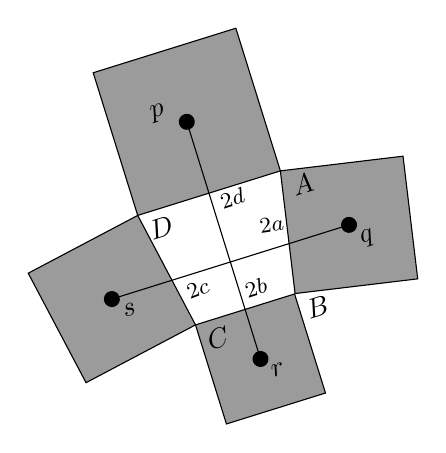
\begin{tikzpicture}[x=0.75pt,y=0.75pt,yscale=-1,xscale=1]
		%uncomment if require: \path (0,300); %set diagram left start at 0, and has height of 300
		
		%Shape: Square [id:dp1824652381634001] 
		\draw  [fill={rgb, 255:red, 155; green, 155; blue, 155 }  ,fill opacity=1 ] (169.06,62.82) -- (237.79,41.37) -- (259.24,110.1) -- (190.51,131.55) -- cycle ;
		%Shape: Square [id:dp8706505809509704] 
		\draw  [fill={rgb, 255:red, 155; green, 155; blue, 155 }  ,fill opacity=1 ] (137.76,159.4) -- (190.51,131.55) -- (218.35,184.3) -- (165.61,212.15) -- cycle ;
		%Shape: Square [id:dp168897752947886] 
		\draw  [fill={rgb, 255:red, 155; green, 155; blue, 155 }  ,fill opacity=1 ] (218.35,184.3) -- (266.08,169.4) -- (280.98,217.13) -- (233.25,232.03) -- cycle ;
		%Shape: Square [id:dp1612401270771493] 
		\draw  [fill={rgb, 255:red, 155; green, 155; blue, 155 }  ,fill opacity=1 ] (259.24,110.1) -- (318.33,103.02) -- (325.41,162.12) -- (266.32,169.2) -- cycle ;
		%Straight Lines [id:da8140206797380386] 
		\draw    (178.06,171.85) -- (292.32,136.11) ;
		\draw [shift={(292.32,136.11)}, rotate = 342.63] [color={rgb, 255:red, 0; green, 0; blue, 0 }  ][fill={rgb, 255:red, 0; green, 0; blue, 0 }  ][line width=0.75]      (0, 0) circle [x radius= 3.35, y radius= 3.35]   ;
		\draw [shift={(178.06,171.85)}, rotate = 342.63] [color={rgb, 255:red, 0; green, 0; blue, 0 }  ][fill={rgb, 255:red, 0; green, 0; blue, 0 }  ][line width=0.75]      (0, 0) circle [x radius= 3.35, y radius= 3.35]   ;
		%Straight Lines [id:da28559875993910744] 
		\draw    (214.15,86.46) -- (249.67,200.72) ;
		\draw [shift={(249.67,200.72)}, rotate = 72.73] [color={rgb, 255:red, 0; green, 0; blue, 0 }  ][fill={rgb, 255:red, 0; green, 0; blue, 0 }  ][line width=0.75]      (0, 0) circle [x radius= 3.35, y radius= 3.35]   ;
		\draw [shift={(214.15,86.46)}, rotate = 72.73] [color={rgb, 255:red, 0; green, 0; blue, 0 }  ][fill={rgb, 255:red, 0; green, 0; blue, 0 }  ][line width=0.75]      (0, 0) circle [x radius= 3.35, y radius= 3.35]   ;
		
		% Text Node
		\draw (194.19,78.44) node [anchor=north west][inner sep=0.75pt]  [rotate=-342.67]  {$p$};
		% Text Node
		\draw (295.25,138.76) node [anchor=north west][inner sep=0.75pt]  [rotate=-342.67]  {$q$};
		% Text Node
		\draw (252.59,203.37) node [anchor=north west][inner sep=0.75pt]  [rotate=-342.67]  {$r$};
		% Text Node
		\draw (180.98,174.5) node [anchor=north west][inner sep=0.75pt]  [rotate=-342.67]  {$s$};
		% Text Node
		\draw (262.16,112.75) node [anchor=north west][inner sep=0.75pt]  [rotate=-342.67]  {$A$};
		% Text Node
		\draw (269.01,172.05) node [anchor=north west][inner sep=0.75pt]  [rotate=-342.67]  {$B$};
		% Text Node
		\draw (221.28,186.95) node [anchor=north west][inner sep=0.75pt]  [rotate=-342.67]  {$C$};
		% Text Node
		\draw (193.43,134.2) node [anchor=north west][inner sep=0.75pt]  [rotate=-342.67]  {$D$};
		% Text Node
		\draw (247.37,132.24) node [anchor=north west][inner sep=0.75pt]  [font=\footnotesize,rotate=-352.11]  {$2a$};
		% Text Node
		\draw (239.78,163.6) node [anchor=north west][inner sep=0.75pt]  [font=\footnotesize,rotate=-342.3]  {$2b$};
		% Text Node
		\draw (211.6,164.92) node [anchor=north west][inner sep=0.75pt]  [font=\footnotesize,rotate=-338.85]  {$2c$};
		% Text Node
		\draw (227.81,120.74) node [anchor=north west][inner sep=0.75pt]  [font=\footnotesize,rotate=-342.4]  {$2d$};
		
		
		\end{tikzpicture}
		
		\end{center}
		
	
	Set $\vec{AB}=2a,\vec{BC}=2b,\vec{CD}=2c,\vec{DA}=2d\quad(a,b,c,d\in \mathrm{C})$
	
	Because A,B,C,D are four vertexes, we have:
	\begin{equation*}
		a+b+c+d=0
	\end{equation*}
	
	Thus: 
	
	\begin{equation*}
		\vec{Aq}=a+ai; \vec{Br}=b+bi; \vec{Cs}=c+ci; \vec{Dp}=d+di
	\end{equation*}
	
	write down $\vec{qs}$:
	
	\begin{equation*}
		\begin{aligned}
		\vec{qs}&=-\vec{Aq}+\vec{AB}+\vec{BC}+\vec{Cs}\\
		        &=(a+2b+c)+i(c-a)\\
		        &=(b-d)+i(c-a)\\
		\vec{rp}&=-\vec{Br}+\vec{BC}+\vec{CD}+\vec{Dp}\\
		        &=(c-a)+i(d-b)
		\end{aligned}
	\end{equation*}
	
	which means
	\begin{equation*}
		i\vec{rp}=\vec{qs},|\vec{rp}|=|\vec{qs}|
	\end{equation*}
	
	So $rp \perp qs$. $\Box$
	
	\subsection{Exercise 1.2}
	set $z_1=a+bi,z_2=c+di$
	
	so 
	\begin{equation*}
		z_1^*z_2=(a-bi)(c+di)=(ac+bd)+i(ad-bc)
	\end{equation*}
	while:
	\begin{equation*}
	\vec{z_1}\cdot \vec{z_2}=(a,b) \cdot (c,d)=ac+bd,\vec{z_1}\times \vec{z_2}=ad-bc
	\end{equation*}
	therefore
	\begin{equation*}
	z_1^*z_2=\vec{z_1}\cdot \vec{z_2}+i\vec{z_1}\times \vec{z_2} \qquad \Box
	\end{equation*}
	
	\subsection{Exercise 1.3}
	The vector space is a group. The identity element is $\vec{0}$, and for any vector $\vec{v}\in V$, the inverse element is $-\vec{v}$.
	
	\subsection{Exercise 1.4}
	The set of all irrational numbers doesn't form a group. There is no identity element  in it. 
	
	\subsection{Exercise 1.5}
	A trivial example is the trivial group with only one element: the identity. 
	
	In classical mechanics, the rotation of a rigid body forms a Lie Group $SO(3)$. And of course $SO(2)$. 
	
	The extended Hamiltonian mechanics present us the symplectic group $Sp(n)$.
	
	In electromagnetics, we have encountered the Lorentz group.
	
	In linear algebra, all isometry forms a group $O(n)$, and of course all $n \times n$ matrices form general linear group $GL(n)$.
	
	\subsection{Exercise 1.6}
	If we have $G \cong H, H \cong I$,which means we have two maps: $f:G\rightarrow H,h:H\rightarrow I$
	
	then :
	\begin{equation*}
	\begin{aligned}
	f(g_1)f(g_2)&=f(g_1g_2)\\
	\Rightarrow h(f(g_1))h(f(g_2))=h(h_1)h(h_2)&=h(h_1h_2)=h(f(g_1)f(g_2))=h(f(g_1g_2))
	\end{aligned}
	\end{equation*}
	
	So the map $h\circ f:G\rightarrow I$ is an isomorphism. which means $G \cong I$. 
	
	It is trivial that a group is isomorphic to itself, which constructs automorphisms. 
	Because the isomorphism is bijective, We can set a inverse map from $H$ to $G$,which means $H \cong G$.
	
	So the isomorphism is an equivalence relation. $\Box$
	
	\subsection{Exercise 1.7}
	Under this multiplication, the identity element is $I(x)=x$. Therefore, we need to find a inverse for $A(X)=(1-x)^{-1}$.
	
	So: $I=B(x)\cdot A(x)=B(A(x))=B((1-x)^{-1})=x$
	
	Solve for $B(x))$:
	\begin{equation*}
		B(x)=\frac{x-1}{x}
	\end{equation*}
	
	Write down its multiplication table:
	\begin{center}
		\begin{tabular}{l|lll}
			\cline{2-4}
			\multicolumn{1}{c|}{}   & \multicolumn{1}{c|}{I} & \multicolumn{1}{c|}{A} & \multicolumn{1}{c|}{B} \\ \hline
			\multicolumn{1}{|l|}{I} & I                      & A                      & B                      \\ \cline{1-1}
			\multicolumn{1}{|l|}{A} & A                      & B                      & I                      \\ \cline{1-1}
			\multicolumn{1}{|l|}{B} & B                      & I                      & A                      \\ \cline{1-1}
		\end{tabular}
	\centerline{group $Z_3$}
	\end{center}
    
    We can find it is actually $Z_3$.
    
    If added $C(x)=x^{-1}$, we have to add at least another two element:
    $D(x)=\frac{x}{x-1},E(x)=1-x$.
    
    If we write down its multiplication table, we have:
    \begin{center}
    	\begin{tabular}{l|llllll}
    		\cline{2-7}
    		& \multicolumn{1}{l|}{I} & \multicolumn{1}{l|}{A} & \multicolumn{1}{l|}{B} & \multicolumn{1}{l|}{C} & \multicolumn{1}{l|}{D} & \multicolumn{1}{l|}{E} \\ \hline
    		\multicolumn{1}{|l|}{I} & I                      & A                      & B                      & C                      & D                      & E                      \\ \cline{1-1}
    		\multicolumn{1}{|l|}{A} & A                      & B                      & I                      & D                      & E                      & C                      \\ \cline{1-1}
    		\multicolumn{1}{|l|}{B} & B                      & I                      & A                      & E                      & C                      & D                      \\ \cline{1-1}
    		\multicolumn{1}{|l|}{C} & C                      & E                      & D                      & I                      & B                      & A                      \\ \cline{1-1}
    		\multicolumn{1}{|l|}{D} & D                      & C                      & E                      & A                      & I                      & B                      \\ \cline{1-1}
    		\multicolumn{1}{|l|}{E} & E                      & D                      & C                      & B                      & A                      & I                      \\ \cline{1-1}
    	\end{tabular}
    \end{center}\textbf{} 
    
    We can see that this group is non-abelian. In general, creating groups by adding generators may make abelian or non-abelian groups. $\Box$
    
\section{Groups, Transformations, and Representations: Some Rudiments}
    \subsection{Exercise 2.1}
    A $4 \times 4$ multiplication table defines two kinds of group.
    
    The first one is $Z_4$,it is abelian. 
    
    \begin{center}
    	\begin{tabular}{l|llll}
    		\cline{2-5}
    		& \multicolumn{1}{l|}{I} & \multicolumn{1}{l|}{A} & \multicolumn{1}{l|}{B} & \multicolumn{1}{l|}{C} \\ \hline
    		\multicolumn{1}{|l|}{I} & I                      & A                      & B                      & C                      \\ \cline{1-1}
    		\multicolumn{1}{|l|}{A} & A                      & B                      & C                      & I                      \\ \cline{1-1}
    		\multicolumn{1}{|l|}{B} & B                      & C                      & I                      & A                      \\ \cline{1-1}
    		\multicolumn{1}{|l|}{C} & C                      & I                      & A                      & B                      \\ \cline{1-1}
    	\end{tabular}
    \centerline{group $Z_4$}
    \end{center}\textbf{} 
    
    The second one is the Vierergruppe, it is also abelian.
    
    \begin{center}
    	\begin{tabular}{l|llll}
    		\cline{2-5}
    		& \multicolumn{1}{l|}{I} & \multicolumn{1}{l|}{A} & \multicolumn{1}{l|}{B} & \multicolumn{1}{l|}{C} \\ \hline
    		\multicolumn{1}{|l|}{I} & I                      & A                      & B                      & C                      \\ \cline{1-1}
    		\multicolumn{1}{|l|}{A} & A                      & I                      & C                      & B                      \\ \cline{1-1}
    		\multicolumn{1}{|l|}{B} & B                      & C                      & I                      & A                      \\ \cline{1-1}
    		\multicolumn{1}{|l|}{C} & C                      & B                      & A                      & I                      \\ \cline{1-1}
    	\end{tabular}
    \centerline{Vierergruppe}
    \end{center}
    
    \subsection{Exercise 2.2}
    The $5 \times 5$ mulitplication table defines only one group :$Z_5$
    
    \begin{center}
    	\begin{tabular}{l|lllll}
    		\cline{2-6}
    		& \multicolumn{1}{l|}{I} & \multicolumn{1}{l|}{A} & \multicolumn{1}{l|}{B} & \multicolumn{1}{l|}{C} & \multicolumn{1}{l|}{D} \\ \hline
    		\multicolumn{1}{|l|}{I} & I                      & A                      & B                      & C                      & D                      \\ \cline{1-1}
    		\multicolumn{1}{|l|}{A} & A                      & B                      & C                      & D                      & I                      \\ \cline{1-1}
    		\multicolumn{1}{|l|}{B} & B                      & C                      & D                      & I                      & A                      \\ \cline{1-1}
    		\multicolumn{1}{|l|}{C} & C                      & D                      & I                      & A                      & B                      \\ \cline{1-1}
    		\multicolumn{1}{|l|}{D} & D                      & I                      & A                      & B                      & C                      \\ \cline{1-1}
    	\end{tabular}
    \centerline{group $Z_5$}
    \end{center}
    
    However, the $6 \times 6$ mulitplication table defines two groups. 
    The first one is $Z_6$:
    
    \begin{center}
    	\begin{tabular}{l|llllll}
    		\cline{2-7}
    		& \multicolumn{1}{l|}{I} & \multicolumn{1}{l|}{A} & \multicolumn{1}{l|}{B} & \multicolumn{1}{l|}{C} & \multicolumn{1}{l|}{D} & \multicolumn{1}{l|}{E} \\ \hline
    		\multicolumn{1}{|l|}{I} & I                      & A                      & B                      & C                      & D                      & E                      \\ \cline{1-1}
    		\multicolumn{1}{|l|}{A} & A                      & B                      & C                      & D                      & E                      & I                      \\ \cline{1-1}
    		\multicolumn{1}{|l|}{B} & B                      & C                      & D                      & E                      & I                      & A                      \\ \cline{1-1}
    		\multicolumn{1}{|l|}{C} & C                      & D                      & E                      & I                      & A                      & B                      \\ \cline{1-1}
    		\multicolumn{1}{|l|}{D} & D                      & E                      & I                      & A                      & B                      & C                      \\ \cline{1-1}
    		\multicolumn{1}{|l|}{E} & E                      & I                      & A                      & B                      & C                      & D                      \\ \cline{1-1}
    	\end{tabular}
    \centerline{group $Z_6$}
    \end{center}
    
    The other one is what we found just in Exercise1.7, it is in fact the group $S_3$, it is the smallest non-abelian group. 
    
    \begin{center}
    	\begin{tabular}{l|llllll}
    		\cline{2-7}
    		& \multicolumn{1}{l|}{I} & \multicolumn{1}{l|}{A} & \multicolumn{1}{l|}{B} & \multicolumn{1}{l|}{C} & \multicolumn{1}{l|}{D} & \multicolumn{1}{l|}{E} \\ \hline
    		\multicolumn{1}{|l|}{I} & I                      & A                      & B                      & C                      & D                      & E                      \\ \cline{1-1}
    		\multicolumn{1}{|l|}{A} & A                      & B                      & I                      & D                      & E                      & C                      \\ \cline{1-1}
    		\multicolumn{1}{|l|}{B} & B                      & I                      & A                      & E                      & C                      & D                      \\ \cline{1-1}
    		\multicolumn{1}{|l|}{C} & C                      & E                      & D                      & I                      & B                      & A                      \\ \cline{1-1}
    		\multicolumn{1}{|l|}{D} & D                      & C                      & E                      & A                      & I                      & B                      \\ \cline{1-1}
    		\multicolumn{1}{|l|}{E} & E                      & D                      & C                      & B                      & A                      & I                      \\ \cline{1-1}
    	\end{tabular}
    	\centerline{$S_3$}
    \end{center}\textbf{}
 
    \subsection{Exercise 2.3}
    Let m,n be a pair of coprime numbers, consider the relation between $Z_m \times Z_n$ and $Z_{m\times n}$.
    
    Because $Z_n$ is a cyclic group, the elements in it can be written as $a^i$, similarly, the elements in $Z_m$ can be written as $b^j$.
    
    So the element in  $Z_m \times Z_n$ can be written as $(a^i,b^j)$. 
    
    the element $(a^i,b^j)^k=(a^{ik},b^{jk})$ must be in  $Z_m \times Z_n$, and if $(a^i,b^j)^k=(a^i,b^j)^l$, which means $a^{ik}=a^{il} \Rightarrow |k-l|=p\times m$, similarly, $|k-l|=q \times n(p,q\in N)$. 
    
    Because m and n coprime with each other, the smallest $ |k-l| $ is $m\times n$.
    So every element in $Z_m \times Z_n$ can be represented as $(a^i,b^j)^k$, it is a (m+n)-order cyclic group, namely $Z_{m\times n}$. 
    
    For m,n have common factors: Set $gcd(m,n)=g$, so the smallest $ |k-l| $ is $\frac{mn}{g}$, which means the element of one cyclic structure cannot fill all elements in the group, which means $Z_m \times Z_n$ is not isomorphic to $Z_{m\times n}$. $\Box$
    
    \subsection{Exercise 2.4}
    The only group of order 7 is $Z_7$, this is abelian. We can prove it by reductio ad absurdum:
    
    If this group is a non-abelian group, then there exist two elements $A,B$, s.t. 
    
    \begin{equation*}
    	\begin{aligned}
    	AB\ne BA
    	\end{aligned}
    \end{equation*}
    
    then: there must be other two elements in the group, namely $C,D$.(If AB=A, then B=I,If AB=I, then A is the inverse of B, which means A and B commute)
    
    Also, the inverse of A and B must in the group, denote them as $A^{-1},B^{-1}$.Then our group looks like $\{I,A,B,AB,BA,A^{-1},B^{-1}\}$, which is exactly 7 elements. 
    
    Because of the closure, $AA$ must be in the group. $AA$ cannot be equal to identity, or $A=A^{-1}$, we have to introduce other elements, which will make the group larger than order-7. $AA$ also cannot be $AB$ or $BA$, otherwise $A=B$. 
    
    So the only possible situation is that $AA=B$, and $BB=A$. However, in this situation:$A=BB=AAAA$ means $I=AAA=AB$, so $B=A^{-1}$, which makes a contradiction. $\Box$
    
    A faster demonstration is through a conclusion: A group with the prime order must be a cyclic group. Next, I will prove it:\\
    \\
    \textbf{Prove}: 
    
     We first prove in finite groups, every element $ a $, if multiplied by itself enough times, it will be equal to the identity. Set $ a $ is an element in a finite group $ G $. The group is order-n. We can multiply $ a $ with itself many many times, and these products must be all in $ G $:
    \begin{equation*}
    \begin{aligned}
    	a,a^2,a^3\cdots a^i \cdots \in G
    \end{aligned}
    \end{equation*}
    
    However, there are only n elements in G,which means in the products of a, there must be at least two elements are equal. Set $a^i=a^j,i<j$, and j is \textbf{the smallest number}  to reach same value \textbf{again}. Here I have to mention that "\textbf{the smallest number}  to reach same value" means in many times of multiplications, there are many chances that two elements are equal, like $a^i=a^j,a^m=a^k...$, but j is the smallest to reach the same again, which means all element before $a^j$ are different. 
    
    If $ i=0 $, which means $ a^i=I $, we have our conclusion. If $i\ne 0$, which means $a^{i-1}\ne a^{j-1}$(because all element before $a^j$ are different). However, we have $a^i=a^j$, if we multiply $ a^{-1} $ on two sides of the equation, we have $a^{i-1}=a^{j-1}$, which contradicts with our previous conclusion. So $ i $ must be 0, which means in a finite group, $\forall a\in G, \exists i\in \mathbb{Z}, a^i=I$, we call this $ i $ the \textbf{order} of an element. 
    
    Next, we shall prove the order of each element must be the factor of the order of the group. 
    
    If the order of the element is i, consider the set $ \{I,a,a^2...a^{i-1}\} $, we can easily check that it indeed form a group, and its a subgroup of $ G $. So according to Lagrange's Thorem, the order of this subgroup divides the order of group $ G $, namely the order of $ a $ divides the order of the group $ G $. 
    
    With this conclusion, we can see that if the group order is a prime number $ p $, the order of each element must be $ 1 $ or $ p $. When the order of the element is $ p $, the group must be with structure  $ \{I,a,a^2...a^{i-1}\} $, which means it's a cyclic group, and of course abelian. \qquad $\Box$
    
    \subsection{Exercise 2.5}
    First: the identity must be in $Z$, because:
    \begin{equation*}
    	Ig=g=gI
    \end{equation*}
    
    Second: the inverse must be in $Z$, because:
    
    if $z_i\in Z$, then $z_ig=gz_i \Rightarrow g=z_igz_i^{-1}$
    
    so:
    
    \begin{equation*}
    	z_i^{-1}g=z_i^{-1}z_igz_i^{-1}=gz_i^{-1}
    \end{equation*}
    
    Third: the composition of any two element is also in $Z$. 
    
    \begin{equation*}
    	z_iz_jg=z_igz_j=gz_iz_j
    \end{equation*}
    
    So $Z$ forms a group. 
    
    Because $g$ is any element in $G$, so 
    
    \begin{equation*}
    	z_iz_j=z_jz_i
    \end{equation*}
    
    which means it is an abelian subgroup.$\Box$ 
    
    \subsection{Exercise 2.6}
    Because the element and its inverse must be in the group, we can pair them together:
    
    \begin{equation*}
    	\{I\},\{A,A^{-1}\},\{B,B^{-1}\}...
    \end{equation*}
    
    Because there is even elements in the group, there must be an element g cannot be paired, which means:
    
    \begin{equation*}
    	g=g^{-1} \Rightarrow gg=I \qquad \Box
    \end{equation*}
    
    However, if the group is of odd order, there may not be such an element(such as $Z_3$). 
    
    \subsection{Exercise 2.7}
    Because the set of words is generated freely by generators, every element in the set can be written as :$\prod_i x_i^{n_i}(n_i\in \mathbb{Z})$. 
    
    First: The identity element is all $n_i=0$, it is of course in the group. 
    
    Second: The inverse of the element $\prod_i x_i^{n_i}$ is $\cdots x_{i+1}^{-n_{i+1}}x_i^{-n_i}\cdots$, which is also in the group. 
    
    Third: The multiplication of two element:
    \begin{equation*}
    	\prod_i x_i^{n_i}\times \prod_j x_i^{m_j}=\prod_i\prod_j x_i^{n_i}x_j^{m_j}
    \end{equation*}
    is also in the group. 
    
    The associativity is trivial. So it forms a group. \qquad $\Box$
    
    \subsection{Exercise 2.8}
    Up to isomorphism, the number of groups with certain order can be solved. 
    
    There are only two kind of 4-order gourp. The first one is $Z_4$, it can be generated by $i$, so the group presentation is :
    \begin{equation*}
    	Z_4=<a| a^4>
    \end{equation*}
    The second group is Vierergruppe, namely $Z_2\times Z_2$, its presentation is:
    \begin{equation*}
      V=<a,b| a^2,b^2,aba^{-1}b^{-1}>
    \end{equation*}
    
    There are only one 5-order group, because 5 is a prime number, it must be a cyclic group. 
    \begin{equation*}
      C_5=Z_5=<a| a^5>
    \end{equation*}
    
    There are two kind of 6-order group. The first is of course $Z_6$, which is isomorphic to $Z_2\times Z_3$:
    \begin{equation*}
      Z_6=<a| a^6>
    \end{equation*}
    The second group is $S_3$, which is the smallest non abelian group:
    \begin{equation*}
      S_3=<a,b| a^2,b^2,(ab)^3,aba=bab>
    \end{equation*}
      Here I choose the cycle $(1,2),(1,3)$ as generators.
      
      I can also choose $(12),(123)$ as group generators, the group presentation will be different:
      \begin{equation*}
      	<a,b|a^2,b^3,(ab)^2>
      \end{equation*}
      
      So we can see that a group can have different presentations. 
      
      
      
    
    
    \subsection{Exercise 2.9}
    We can write two representations of $\mathbb{Z}$:
    for a,b two integers, we have: 
    \begin{equation*}
      \begin{pmatrix}
      1 & a\\
      0 & 1
      \end{pmatrix}
      \begin{pmatrix}
      1 & b\\
      0 & 1
      \end{pmatrix}
      =
      \begin{pmatrix}
      1 & a+b\\
      0 & 1
      \end{pmatrix}
    \end{equation*}
    also, we have:
    \begin{equation*}
    \begin{pmatrix}
    1 & 0\\
    a & 1
    \end{pmatrix}
    \begin{pmatrix}
    1 & 0\\
    b & 1
    \end{pmatrix}
    =
    \begin{pmatrix}
    1 & 0\\
    a+b & 1
    \end{pmatrix}
    \end{equation*}
    
    So 
    \begin{equation*}
      \begin{pmatrix}
      1 & a\\
      0 & 1
      \end{pmatrix}
      \rm{and}
      \begin{pmatrix}
      1 & 0\\
      a & 1
      \end{pmatrix}
    \end{equation*}
    are two representations of $\mathbb{Z}$. 
    These two representations are equaivalent. 
    
    \textbf{Proof:}
    
    Consider matrix:
    \begin{equation*}
      P=\begin{pmatrix}
      0 & 1\\
      1 & 0
      \end{pmatrix}
      =
      \begin{pmatrix}
      0 & 1\\
      1 & 0
      \end{pmatrix}
      ^{-1}
    \end{equation*}
    
    We can use this matrix to transform:
    \begin{equation*}
      \begin{pmatrix}
      1 & 0\\
      a & 1
      \end{pmatrix}
      =
      \begin{pmatrix}
      0 & 1\\
      1 & 0
      \end{pmatrix}
      \begin{pmatrix}
      1 & a\\
      0 & 1
      \end{pmatrix}
      \begin{pmatrix}
      0 & 1\\
      1 & 0
      \end{pmatrix}
      ^{-1}
    \end{equation*}
    This is a similarity transformation. So we are done, these two representations are equivalent. \qquad $\Box$
    
    However, in general, how can we determine whether two reps are equivalent? It is not equal to deciding whether two matrices are similar, because if the transformation matrix is involved with the group element, for example, if in this case, $P$ is involved with the parameter $a$, you can not say these two reps are equivalent because the transformation matrix isn't a constant matrix.
    
    Of course, using Great Orthogonality Theorem: 
    \begin{equation*}
    	\sum_g D^{(r)\dagger}(g)_j^i D^{(s)}(g)_l^k=\frac{N(G)}{d_r} \delta^{rs} \delta^i_l \delta^k_j
    \end{equation*}
    we can easily check two irrep $r,s$ are equivalent or not. However we haven't studied it yet. We may find a more elementry way. 
    
    We shall first consider a weaker question: How can we determine if two matrix are similar? \\
    \textbf{Lemma:} Two square matrices are similar if and only if they have the same Jordan normal form.
    
    we can prove it through  algebric proof or the solutions of associated linear differential equations. Here we present the former.
    
    The Jordan normal form tell us that any matrix can be decomposed into:
    \begin{equation*}
    	T^{-1}AT=
    	\begin{pmatrix}
    	L_{k_1}(\lambda_1)&0&0&0\\
    	0&L_{k_2}(\lambda_2)&0&0\\
    	0&0&\ddots          &0\\
    	0&0&0&L_{k_r}(\lambda_r) 
    	\end{pmatrix}
    \end{equation*}
    where $L_k(\lambda)$ is a $k\times k$ matrix: 
    \begin{equation*}
    	L_k(\lambda)=
    	\begin{pmatrix}
    	\lambda&1&0&\cdots&0\\
    	0&\lambda&1&\cdots&0\\
    	\vdots&\quad&\ddots&\ddots&\vdots\\
    	\vdots&\quad&\quad&\ddots&1\\
    	0&0&0&\cdots&\lambda
    	\end{pmatrix}
    \end{equation*}
    
    So if $A\sim B$, then there exists an invertible matrix $S$, s.t.
    \begin{equation*}
      B=SAS^{-1}=STLT^{-1}S^{-1}=(ST)L(ST)^{-1}
    \end{equation*}
    So B has the same Jordan normal form with A. 
    
    Conversely, if A and B share the same Jordan normal form, namely:
    \begin{equation*}
    \begin{aligned}
     L&=TAT^{-1}=PBP^{-1}\\
     \Rightarrow B&=P^{-1}TAT^{-1}P=(P^{-1}T)A(P^{-1}T)^{-1}
    \end{aligned}
    \end{equation*}
    It is obvious that $P^{-1}T$ is an invertible matrix, so $B\sim A$. \qquad $\Box$
    
    So, when it comes to two reps, we can first check whether their Jordan normal form are identical, then check whether their transformation matrix is involved with the group element. 
    
    Exempli gratia, the Jordan normal form for A and B are:
    \begin{equation*}
    A=
    \begin{pmatrix}
    1 & a\\
    0 & 1
    \end{pmatrix}
    =
    \left(
    \begin{array}{cc}
    1 & 0 \\
    0 & \frac{1}{a} \\
    \end{array}
    \right).\left(
    \begin{array}{cc}
    1 & 1 \\
    0 & 1 \\
    \end{array}
    \right).\left(
    \begin{array}{cc}
    1 & 0 \\
    0 & \frac{1}{a} \\
    \end{array}
    \right)^{-1}
    \end{equation*}
    and
    \begin{equation*}
    	B=
    	\begin{pmatrix}
    	1 & 0\\
    	a & 1
    	\end{pmatrix}
    	=
    	\left(
    	\begin{array}{cc}
    	0 & \frac{1}{a} \\
    	1 & 0 \\
    	\end{array}
    	\right).\left(
    	\begin{array}{cc}
    	1 & 1 \\
    	0 & 1 \\
    	\end{array}
    	\right).\left(
    	\begin{array}{cc}
    	0 & \frac{1}{a} \\
    	1 & 0 \\
    	\end{array}
    	\right)^{-1}
    \end{equation*}
    
    We can see that A and B share the same Jordan normal form, so $A\sim B$, But we kant say that these two reps are equivalent because the transformation matix are involved with the group element $a$. But if we write down the transformation matrix between A and B, we can see:
    \begin{equation*}
    \begin{aligned}
    	B=(P^{-1}T)A(P^{-1}T)^{-1}&=
    	\left(
    	\begin{array}{cc}
    	0 & \frac{1}{a} \\
    	1 & 0 \\
    	\end{array}
    	\right)
    	\left(
    	\begin{array}{cc}
    	1 & 0 \\
    	0 & \frac{1}{a} \\
    	\end{array}
    	\right)^{-1}
    	\left(
    	\begin{array}{cc}
    	1 & a \\
    	0 & 1 \\
    	\end{array}
    	\right)
    	\left(
    	\begin{array}{cc}
    	1 & 0 \\
    	0 & \frac{1}{a} \\
    	\end{array}
    	\right)
    	\left(
    	\begin{array}{cc}
    	0 & \frac{1}{a} \\
    	1 & 0 \\
    	\end{array}
    	\right)^{-1}\\
    	&=\begin{pmatrix}
    	0 & 1\\
    	1 & 0
    	\end{pmatrix}
    	\begin{pmatrix}
    	1 & a\\
    	0 & 1
    	\end{pmatrix}
    	\begin{pmatrix}
    	0 & 1\\
    	1 & 0
    	\end{pmatrix}
    	^{-1}
    \end{aligned}
    \end{equation*}
    
    Woo, the transformation matrix between A and B gets rid of the group element a! So these two reps are equivalent. \qquad $\Box$
    
    So in general, if we want to know whether two reps are euqivalent or not, we can first write down its Jordan normal form to determine whether two matrix are similar, then multiply their Jordan Basis together to see if it is involved with the group element. 
    
    However in this simple case, we can just solve the transformation matrix directly, set:
    
    \begin{equation*}
    \begin{aligned}
    S=
    \begin{pmatrix}
    x & m\\
    y & n
    \end{pmatrix}
    \end{aligned}
    \end{equation*}
    
    so:
    \begin{equation*}
    \begin{aligned}
    SA&=BS\\
    \Rightarrow \begin{pmatrix}
    x & m\\
    y & n
    \end{pmatrix}
    \begin{pmatrix}
    1 & a\\
    0 & 1
    \end{pmatrix}
    &=
    \begin{pmatrix}
    1 & 0\\
    a & 1
    \end{pmatrix}
    \begin{pmatrix}
    x & m\\
    y & n
    \end{pmatrix}\\
    \Rightarrow \begin{pmatrix}
    x & ax+m\\
    y & ay+n
    \end{pmatrix}
    &=
    \begin{pmatrix}
    x & m\\
    ax+y & am+n
    \end{pmatrix}\\
    \Rightarrow S&=
    \begin{pmatrix}
    0 & m\\
    m & n
    \end{pmatrix}\\
    {\rm Set\quad  m=1,n=0}\Rightarrow S&=
    \begin{pmatrix}
    0 & 1\\
    1 & 0
    \end{pmatrix}
    \end{aligned}
    \end{equation*}
    Which is easier when rep is in a low dimension. \qquad $ \Box $ 
    
    \subsection{Exercise 2.10}
    We can set $M\in U(N)$ as follows:
    \begin{equation*}
      M=
      \begin{pmatrix}
      a+bi & c+di&\cdots\\
      e+fi & \ddots&\vdots\\
      \vdots&\cdots
      \end{pmatrix}
    \end{equation*}
    Theer are $2N^2$ real parameters. 
    
    With its definition:
    \begin{equation*}
      M^{\dagger}M=I
    \end{equation*}
    We have $N^2$ equations, namely $N^2$ restrictions. So the dimension of group $U(N)$ is $2N^2-N^2=N^2$.
    
    Similarly, we can find other Lie group's demension by this method:
    \begin{center}
    	\begin{tabular}{|l|l|l|l|}
    		\hline
    		\textbf{Name of the group}  & \textbf{Properites}             & \textbf{Dimension} & \textbf{Algebra}                  \\ \hline
    		\textbf{$O(n)$}             & $O^TO=I$                        & $\frac{n(n-1)}{2}$ & anti-symmetric matrices           \\ \hline
    		\textbf{$SO(n)$}            & $O^TO=I$ and $det(O)=1$         & $\frac{n(n-1)}{2}$ & anti-symmetric matrices           \\ \hline
    		\textbf{$U(n)$}             & $U^{\dagger}U=I$                & $n^2$              & anti-hermitian matrices           \\ \hline
    		\textbf{$SU(n)$}            & $U^{\dagger}U=I$ and $det(U)=1$ & $n^2-1$            & traceless anti-symmetric matrices \\ \hline
    		\textbf{$SL(n,\mathbb{R})$} & $det(L)=1$                      & $n^2-1$            & traceless real matrices           \\ \hline
    		\textbf{$SL(n,\mathbb{C})$} & $det(L)=1$                      & $2(n^2-1)$         & traceless complex matrices        \\ \hline
    	\end{tabular}
    \centerline{common Lie groups and their property}
    \end{center}
    
    \subsection{Exercise 2.11}
    No. Such as $Z_3$ is not any subgroup of a free group. With the same group multiplication, the bigger group must have the relation $e^3=I$, so the bigger group is not a free group. 
    
    \subsection{Exercise 2.12}
    The multiplication table for $D_4$ is as follows:
    \begin{equation*}
    	\begin{array}{|c|c|c|c|c|c|c|c|c|}
    	\hline D_4& e & b & a & a^{2} & a^{3} & a b & a^{2} b & a^{3} b \\
    	\hline e & e & b & a & a^{2} & a^{3} & a b & a^{2} b & a^{3} b \\
    	\hline b & b & e & a^{3} b & a^{2} b & a b & a^{3} & a^{2} & a \\
    	\hline a & a & a b & a^{2} & a^{3} & e & a^{2} b & a^{3} b & b \\
    	\hline a^{2} & a^{2} & a^{2} b & a^{3} & e & a & a^{3} b & b & a b \\
    	\hline a^{3} & a^{3} & a^{3} b & e & a & a^{2} & b & a b & a^{2} b \\
    	\hline a b & a b & a & b & a^{3} b & a^{2} b & e & a^{3} & a^{2} \\
    	\hline a^{2} b & a^{2} b & a^{2} & a b & b & a^{3} b & a & e & a^{3} \\
    	\hline a^{3} b & a^{3} b & a^{3} & a^{2} b & a b & b & a^{2} & a & e \\
    	\hline
    	\end{array}
    \end{equation*}
    
    The presentation of $D_4$ is:
    \begin{equation*}
      <r,f|r^4,f^2,(rf)^2>
    \end{equation*}
    
    The multiplication table is not symmetric, so it is not abelian. 
    
    \subsection{Exercise 2.13}
    The multiplication table of $D_3$ has already appeared before. If we change the name of the element, r represents the rotation and s represents the reflection:
    \begin{equation*}
    	\begin{array}{|l|l|l|l|l|l|l|}
    	\hline D_3 & \mathrm{r}_{0} & \mathrm{r}_{1} & \mathrm{r}_{2} & \mathrm{s}_{0} & \mathrm{s}_{1} & \mathrm{s}_{2} \\
    	\hline \mathrm{r}_{0} & \mathrm{r}_{0} & \mathrm{r}_{1} & \mathrm{r}_{2} & \mathrm{s}_{0} & \mathrm{s}_{1} & \mathrm{s}_{2} \\
    	\hline \mathrm{r}_{1} & \mathrm{r}_{1} & \mathrm{r}_{2} & \mathrm{r}_{0} & \mathrm{s}_{1} & \mathrm{s}_{2} & \mathrm{s}_{0} \\
    	\hline \mathrm{r}_{2} & \mathrm{r}_{2} & \mathrm{r}_{0} & \mathrm{r}_{1} & \mathrm{s}_{2} & \mathrm{s}_{0} & \mathrm{s}_{1} \\
    	\hline \mathrm{s}_{0} & \mathrm{s}_{0} & \mathrm{s}_{2} & \mathrm{s}_{1} & \mathrm{r}_{0} & \mathrm{r}_{2} & \mathrm{r}_{1} \\
    	\hline \mathrm{s}_{1} & \mathrm{s}_{1} & \mathrm{s}_{0} & \mathrm{s}_{2} & \mathrm{r}_{1} & \mathrm{r}_{0} & \mathrm{r}_{2} \\
    	\hline \mathrm{s}_{2} & \mathrm{s}_{2} & \mathrm{s}_{1} & \mathrm{s}_{0} & \mathrm{r}_{2} & \mathrm{r}_{1} & \mathrm{r}_{0} \\
    	\hline
    	\end{array}
    \end{equation*}
    
    The presentation is similar to $D_4$:
    \begin{equation*}
    	<r,f|r^3,s^2,(rs)^2>
    \end{equation*}
    
    \subsection{Exercise 2.14}
    In fact, I don't really know what "defining" really means, since physicsts never say or define things clearly for their "intuitive clearness".  I just assume the defining rep of $D_n$ as the subrepresentation of $O(n)$.
    
    So the defing rep of $ D_3 $ maybe:
    \begin{equation*}
    	\begin{aligned}
    	\mathbf{r}_{0} &=\left(\begin{array}{cc}
    	1 & 0 \\
    	0 & 1
    	\end{array}\right), \mathbf{r}_{1} =\left(\begin{array}{cc}
    	-\frac{1}{2} & -\frac{\sqrt{3}}{2} \\
    	\frac{\sqrt{3}}{2} & -\frac{1}{2}
    	\end{array}\right), \mathbf{r}_{2} =\left(\begin{array}{cc}
    	-\frac{1}{2} & \frac{\sqrt{3}}{2} \\
    	-\frac{\sqrt{3}}{2} & -\frac{1}{2}
    	\end{array}\right)\\
    	\mathbf{s}_{0} &=\left(\begin{array}{cc}
    	1 & 0 \\
    	0 & -1
    	\end{array}\right), \mathbf{s}_{1}=\left(\begin{array}{cc}
    	-\frac{1}{2} & \frac{\sqrt{3}}{2} \\
    	\frac{\sqrt{3}}{2} & \frac{1}{2}
    	\end{array}\right), \mathbf{s}_{2}=\left(\begin{array}{cc}
    	-\frac{1}{2} & -\frac{\sqrt{3}}{2} \\
    	-\frac{\sqrt{3}}{2} & \frac{1}{2}
    	\end{array}\right)
    	\end{aligned}
    \end{equation*}
    
    The defining rep of $ D_4 $ may be:
    \begin{equation*}
    	\begin{aligned}
    	\mathbf{r}_{0} &=\left(\begin{array}{cc}
    	1 & 0 \\
    	0 & 1
    	\end{array}\right),& \mathbf{r}_{1}=\left(\begin{array}{cc}
    	0 & -1 \\
    	1 & 0
    	\end{array}\right),& \mathbf{r}_{2}=\left(\begin{array}{cc}
    	-1 & 0 \\
    	0 & -1
    	\end{array}\right),& \mathbf{r}_{3}=\left(\begin{array}{cc}
    	0 & 1 \\
    	-1 & 0
    	\end{array}\right) \\
    	\mathbf{s}_{0} &=\left(\begin{array}{cc}
    	1 & 0 \\
    	0 & -1
    	\end{array}\right),& \mathbf{s}_{1}=\left(\begin{array}{cc}
    	0 & 1 \\
    	1 & 0
    	\end{array}\right),& \mathbf{s}_{2}=\left(\begin{array}{cc}
    	-1 & 0 \\
    	0 & 1
    	\end{array}\right),& \mathbf{s}_{3}=\left(\begin{array}{cc}
    	0 & -1 \\
    	-1 & 0
    	\end{array}\right)
    	\end{aligned}
    \end{equation*}
    
    The defining rep of $ D_n $ may be:
    \begin{equation*}
    	\begin{aligned}\mathbf {r} _{k}&={\begin{pmatrix}\cos {\frac {2\pi k}{n}}&-\sin {\frac {2\pi k}{n}}\\\sin {\frac {2\pi k}{n}}&\cos {\frac {2\pi k}{n}}\end{pmatrix}}\ \ {\text{and}}\quad \mathbf {s} _{k}&={\begin{pmatrix}\cos {\frac {2\pi k}{n}}&\sin {\frac {2\pi k}{n}}\\\sin {\frac {2\pi k}{n}}&-\cos {\frac {2\pi k}{n}}\end{pmatrix}}\end{aligned}
    \end{equation*}
    
    Can we define what is "defining", please?
    
    \subsection{Exercise 2.15}
    For every dihidral group, their presentation can be written as:
    \begin{equation*}
      D_n=<r,f|r^n,f^2,(rf)^2>
    \end{equation*}
    
    So, there is no general difference between $D_{2n}$ and $D_{2n+1}$.
    
    \subsection{Exercise 2.16}
    Since $H$ is a subgroup of $ G $, the set $ g^{-1}Hg $ can be written as:
    \begin{equation*}
      g^{-1}Hg=\{g^{-1}h_1g,g^{-1}h_2g,g^{-1}h_3g...\}
    \end{equation*}
    
    First: The Identity $ I $ must be in group $ H $:
    \begin{equation*}
      g^{-1}Ig=g^{-1}g=I\in g^{-1}Hg
    \end{equation*}
    
    Second: For an element $ g^{-1}h_ig $, its inverse:
    \begin{equation*}
      (g^{-1}h_ig)^{-1}=g^{-1}h_1^{-1}g\in g^{-1}Hg
    \end{equation*}
    
    Third: For two element $ g^{-1}h_1g $,$  g^{-1}h_2g $, their multiplication is also in the group:
    \begin{equation*}
      (g^{-1}h_1g)(g^{-1}h_2g)=g^{-1}h_2gg^{-1}h_2g=g^{-1}h_1h_2g\in g^{-1}Hg
    \end{equation*}
    
    So $ g^{-1}Hg $ forms a group. \qquad $ \Box $
    
    \subsection{Exercise 2.17}
    Group $ G_{i} $ have one invariant subgroup:
    \begin{equation*}
      Z_2=\{1,-1\}\lhd G_{i}
    \end{equation*}
    
    First, the four elements in $ G_{i} $ can be treated as four rotation elements in $ D_4 $, so $  G_{i} $ is isomorphic to a subgroup of $ D_4 $. Denote the four elements in $ G_{i} $ as $ a_1,a_2,a_3,a_4 $. First, according to the rearrangement lemma, $ G_{i} $ itself must be the invariant subgroup of $ G_{i} $. Let's check its other cosets:
    \begin{equation*}
      \begin{aligned}
      b_1G_{i}&=\{b_1,b_1a_1,b_1a_2,b_1a_3\}\\
              &=\{b_1,a_3b_1,a_2b_1,a_1b_1\}=G_{i}b_1\\
      b_2G_{i}&=\{b_2,b_2a_1,b_2a_2,b_2a_3\}\\
              &=\{b_2,b_1,a_3b_1,a_2b_1\}\\
              &=\{b_2,a_3b_2,a_2b_2,a_1b_2\}=G_{i}b_2\\
      b_3G_{i}&=\{b_3,b_3a_1,b_3a_2,b_3a_3\}\\
              &=\{b_3,a_1b_1,b_1,a_3b_1\}\\
              &=\{b_3,a_3b_3,a_2b_3,a_1b_3\}=G_{i}b_3\\
      b_4G_{i}&=\{b_4,b_4a_1,b_4a_2,b_4a_3\}\\
              &=\{b_4,a_2b_1,a_1b_1,b_1\}\\
              &=\{b_4,a_3b_4,a_2b_4,a_1b_4\}=G_{i}b_4\\
      \end{aligned}
    \end{equation*}
    
    Here we define $ b_1=b, b_2=a_1b, b_3=a_2b, b_4=a_3b $ from our multiplication table in Exercise 2.12.We can see that for every element in $D_4$, their left cosets equal to their right cosets. Therefore, $ G_{i}\lhd D_4 $. \qquad $ \Box $
    
    $ D_3 $ has invariant subgroup, see Exercise 2.20.  
    
    \subsection{Exercise 2.18}
    It is toooo trivial to prove for a normal subgroup, the cosets form a group. I'm getting bored:
    
    Frist: The identity element is $ H $.
    
    Second: The inverse of $ gH $ is $ g^{-1}H $.
    
    Third: It is closure: $ g_1Hg_2H=(g_1g_2)H=g_3H $.
    
    So it forms a group, the quotient group. \qquad $ \Box $
    
    \subsection{Exercise 2.19}
    $ kerf $ is a group:
    
    First: The identity element is in it:
    \begin{equation*}
    f(I)=f(II)=f(I)f(I)\Rightarrow f(I)=0\Rightarrow I\in kerf
    \end{equation*}
    
    Second: For every element $ x\in kerf $, $ x^{-1} $ must in $ kerf $:
    \begin{equation*}
    f(x^{-1})=f(x)f(x^{-1})=f(I)=0\Rightarrow x^{-1}\in kerf
    \end{equation*}
    
    Third: For every two elements in $ kerf $:
    \begin{equation*}
    f(ab)=f(a)f(b)=0\Rightarrow ab\in kerf
    \end{equation*}
    
    So $ kerf $ forms a group.
    
    $ imf $ is a group:
    
    First: The identity element is in it:
    \begin{equation*}
    f(I)=0\in imf
    \end{equation*}
    
    Second: The inverse element is in it:
    \begin{equation*}
    f(I)=f(xx^{-1})=f(x)f(x^{-1})\in imf\Rightarrow f(x^{-1})\in imf
    \end{equation*}
    
    Third: For every two element in $imf$:
    \begin{equation*}
    f(a)f(b)=f(ab)\in imf
    \end{equation*}
    
    So $ imf $ forms a group. \qquad $ \Box $
    
    \subsection{Exercise 2.20}
    There are 4 non trivial subgroups in $ D_3 $:
    \begin{equation*}
    \begin{aligned}
      H_1&=\{r_0,s_1\}\\
      H_2&=\{r_0,s_2\}\\
      H_3&=\{r_0,s_3\}\\
      H_4&=\{r_0,r_1,r_2\}
    \end{aligned}
    \end{equation*}
    $ H_1,H_2,H_3 $ are not invariant subgroups,but $ H_4 $ is an invariant subgroup of $ D_3 $, we can prove it just like before. In fact, it is $ A_3 \lhd S_3 $. 
    
    When we want to write down its quotient group $ D_3/H_4 $, we may write down for the first sight:
    \begin{equation*}
      \{H_4=\{r_0,r_1,r_2\},s_1H_4=\{s_1,s_3\},s_2H_4=\{s_1,s_2\},s_3H_4=\{s_2,s_3\}\}
    \end{equation*}
    However, it is wrong, because if you try to find the inverse of some elements, you may find more than one inverse:
    \begin{equation*}
      s_1H_4s_1H_4=H_4=s_1H_4s_2H_4=s_1H_4s_3H_4
    \end{equation*}
    So $ s_1H_4,s_1H_4,s_1H_4 $ are actually the same element. Then $ D_3/H_4 $ should be
    \begin{equation*}
      \{H_4,s_1H_4\}\cong Z_2
    \end{equation*}
    
    $ D_4 $ is a pretty interesting group, it has 8 subgroups:
    \begin{equation*}
    \begin{aligned}
      H_1&=\{I,b_1\}\cong Z_2\\
      H_2&=\{I,b_2\}\cong Z_2\\
      H_3&=\{I,b_3\}\cong Z_2\\
      H_4&=\{I,b_4\}\cong Z_2\\
      H_5&=\{I,a_2\}\cong Z_2\\
      H_6&=\{I,a_1,a_2,a_3\}\cong Z_4\\
      H_7&=\{I,a_2,b_1,b_3\}\cong Z_2\times Z_2\\
      H_8&=\{I,a_2,b_2,b_4\}\cong Z_2\times Z_2
    \end{aligned}
    \end{equation*}
    
    We have already known that $ H_6 $ is an invariant subgroup of $ D_4 $, thus the quotient group:
    \begin{equation*}
      D_4/Z_4\cong Z_2
    \end{equation*}
    
    What about other subgroups? It seems obvious that $ H_5=\{I,a_2\} $ is a invariant subgroup of $ D_4 $. So its quotient group is:
    \begin{equation*}
      D_4/H_5=\{H_5,b_1H_5,b_2H_5,b_4H_5\}\cong Z_2\times Z_2
    \end{equation*}
    (Deciding the element and the structure of the quotient group is killing me...I spent a lot time on it...)
    
    We can also find the $ H_7=\{I,a_2,b_1,b_3\},H_8=\{I,a_2,b_2,b_4\} $ are also two normal subgroups of $ D_4 $,their quotient group are both isomorphic to $ Z_2 $
    \begin{equation*}
    \begin{aligned}
    D_4/H_7\cong Z_2\\
    D_4/H_8\cong Z_2
    \end{aligned}
    \end{equation*}
    
    So in all, $ D_4 $ has 4 invariant subgroups, they are:
    \begin{equation*}
      \begin{aligned}
      H_5&=\{I,a_2\}\cong Z_2\\
      H_6&=\{I,a_1,a_2,a_3\}\cong Z_4\\
      H_7&=\{I,a_2,b_1,b_3\}\cong Z_2\times Z_2\\
      H_8&=\{I,a_2,b_2,b_4\}\cong Z_2\times Z_2\qquad \Box
      \end{aligned}
    \end{equation*}
    
    An interesting thing is that it seems for a normal subgroup $ H $, the quotient group $ G/H $ may be isomorphic to a subgroup of $ G $, and I think its a good exercise to prove it or find a counter-example.
    
    
    \subsection{Exercise 2.21}
		Set:
		\begin{equation*}
		\begin{aligned}
		f:G\rightarrow G, x\in \operatorname{ker}(f)=K
		\end{aligned}
		\end{equation*}
		To show that $K$ is an invariant subgroup, we want to show that: for any $g\in G$, s.t. $gxg^{-1}\in K$
		
		We have
		\begin{equation*}
		\begin{aligned}
		f(gxg^{-1})=f(g)f(x)f(g^{-1})&=f(g)f(g^{-1})=f(gg^{-1})=I\\
		\Rightarrow gxg^{-1}&\in K
		\end{aligned}
		\end{equation*}
		So $K$ is an invariant subgroup, and the homomorphism need't be $G\rightarrow G.\qquad \Box$
		
		\subsection{Exercise 2.22}
		We should make an homomorphism between $ G/\operatorname{ker}(f) $ and $ \operatorname{im}(f) $ and show it is bijective:
		
		Define: $ i:G/\operatorname{ker}(f)\rightarrow \operatorname{im}(f) $,s.t.:
		\begin{equation*}
		i(g\operatorname{ker}(f))=f(g)
		\end{equation*}
		
		We first prove it is well defined: if $a\operatorname{ker}(f)=b\operatorname{ker}(f)$, then $i(a\operatorname{ker}(f))=i(b\operatorname{ker}(f))$
		\begin{equation*}
		\begin{aligned}
		a\operatorname{ker}(f)&=b\operatorname{ker}(f)\\
		\Rightarrow b^{-1}a\operatorname{ker}(f)&=\operatorname{ker}(f)\\
		\Rightarrow b^{-1}a&\in \operatorname{ker}(f)\rm{(rearrangement\quad lemma)}\\ 
		0=f(b^{-1}a)&=f(b^{-1})f(a)=f^{-1}(b)f(a)\\
		\Rightarrow f(a)&=f(b)\\
		\Rightarrow i(a\operatorname{ker}(f))=f(a)&=f(b)=i(b\operatorname{ker}(f))
		\end{aligned}
		\end{equation*}
		
		We secondly prove that $ i $ is a homomorphism, namely:$ i(a\operatorname{ker}(f))i(b\operatorname{ker}(f))=i(a\operatorname{ker}(f)\cdot b\operatorname{ker}(f)) $
		\begin{equation*}
		\begin{aligned}
		i(a\operatorname{ker}(f))i(b\operatorname{ker}(f))&=f(a)f(b)\\
		&=f(ab)\\
		&=i(ab\operatorname{ker}(f))\\
		&=i(a\operatorname{ker}(f)\cdot b\operatorname{ker}(f))\\
		\end{aligned}
		\end{equation*}
		So $ i $ is an homomorphism.
		
		Then we show $ i $ is an \textbf{i}somorphism:
		
		If $ f(a)\in \operatorname{im}(f), \Rightarrow \exists a\operatorname{ker}(f)\in G/\operatorname{ker}(f),{\rm s.t. } i(a\operatorname{ker}(f))=f(a)$, so it is surjective. 
		
		If $ i(a\operatorname{ker}(f))=i(b\operatorname{ker}(f)) $
		then:
		\begin{equation*}
		\begin{aligned}
		&f(a)=f(b)\\
		\Rightarrow &f^{-1}(b)f(a)=0\\
		\Rightarrow &f(b^{-1})f(a)=0\\
		\Rightarrow &f(b^{-1}a)=0\\
		\Rightarrow &b^{-1}a\in \operatorname{ker}(f)\\
		\Rightarrow &b^{-1}a\operatorname{ker}(f)=\operatorname{ker}(f)\\
		\Rightarrow &a\operatorname{ker}(f)=b\operatorname{ker}(f)\\
		\end{aligned}
		\end{equation*}
		So it is injective.
		
		This homomorphism is into and onto, so $G/\operatorname{ker}(f)\cong \operatorname{im}(f)$
		
		\subsection{Exercise 2.23}
		Because
		\begin{equation*}
		\begin{aligned}
		&f_2: G_2\rightarrow e\\
		\Rightarrow & \operatorname{ker}(f_2)=G_2\\
		\Rightarrow & G_2=\operatorname{ker}(f_2)=\operatorname{im}(f_1)
		\end{aligned}
		\end{equation*}
		So $ f_1 $ is surjective.
		
		Because:
		\begin{equation*}
		\begin{aligned}
		&f_0:e\rightarrow G_1\\
		\Rightarrow & f_0(e)=I\\
		\Rightarrow & \operatorname{ker}(f_1)=\operatorname{im}(f_0)=\{I\}\\
		\end{aligned}
		\end{equation*} 
		So $f_1$ is injective.Thus $ f_1 $ is an isomorphism. \qquad $ \Box $
		
		\subsection{Exercise 2.24}
		Because of the fundamental theorem of homomorphism:
		\begin{equation*}
		G_2/\operatorname{ker}(f_2)\cong \operatorname{im}(f_2)
		\end{equation*}
		We want to prove that: $\operatorname{im}(f_2)\cong G_3$ and $\operatorname{ker}(f_2)\cong G_1$.
		
		Because:
		\begin{equation*}
		\begin{aligned}
		&f_3: G_3\rightarrow e\\
		\Rightarrow & \operatorname{ker}(f_3)=G_3\\
		\Rightarrow & \operatorname{im}(f_2)=\operatorname{ker}(f_3)=G_3
		\end{aligned}
		\end{equation*}
		
		And:
		\begin{equation*}
		\begin{aligned}
		&f_0:e\rightarrow G_1\\
		\Rightarrow & f_0(e)=I\\
		\Rightarrow & \operatorname{ker}(f_1)=\operatorname{im}(f_0)=\{I\}\\
		{\rm with}\quad & G_1/\operatorname{ker}(f_1)\cong \operatorname{im}(f_1)\\
		\Rightarrow & G_1/\{I\}\cong \operatorname{im}(f_1)= \operatorname{ker}(f_2)\\
		\Rightarrow & G_1\cong \operatorname{ker}{f_2}
		\end{aligned}
		\end{equation*}
		
		Therefore
		\begin{equation*}
		G_2/G_1\cong G_3\qquad \Box
		\end{equation*}

     
    
    \subsection{Exercise 2.25}
    \begin{equation*}
    \begin{aligned}
    &\mathbb{R}/\mathbb{Z}=\{\mathbb{Z},a+\mathbb{Z}\}(a\in (0,1))\\
    \Rightarrow &\exists {\rm isomorphism}f:\mathbb{R}/\mathbb{Z}\rightarrow [0,1)\\
    \Rightarrow &\exists {\rm isomorphism}g:\mathbb{R}/\mathbb{Z}\rightarrow e^{i\phi}{(\rm \exists h:[0,1)\rightarrow e^{i\phi})}\\
    \Rightarrow & \mathbb{R}/\mathbb{Z}\cong U(1)\qquad \Box
    \end{aligned}
    \end{equation*}
    
    \subsection{Exercise 2.26}
    The presentation of $\mathbb{H}$ can be witten as:
    \begin{equation*}
    \mathbb{H}=<\mi,\mj,\mk|\mi^2=\mj^2=\mk^2=\mi\mj\mk=-1>
    \end{equation*}
    
    \subsection{Exercise 2.27}
		Because of the symmetry, we can only consider $\mj$ acts on $Z_4$:
		\begin{equation*}
			\mj Z_4\mj^{-1}=\mj\{1,-1,\mi,-\mi\}-\mj=\{1,-1,\mi,-\mi\}
		\end{equation*}
		
		so $Z_4$ is an invariant subgroup of $\mathbb{H}$. 
	
	\subsection{Exercise 2.28}
		If we set a map: $\mi\mapsto \mi\sigma_z,\mj\mapsto \mi\sigma_y,\mk\mapsto \mi\sigma_x$, we can check that:
		\begin{equation*}
			(\mi\sigma_z)^2=(\mi\sigma_y)^2=(\mi\sigma_x)^2=(\mi\sigma_z)(\mi\sigma_y)(\mi\sigma_x)=-I
		\end{equation*}
		For example: 
		\begin{equation*}
		\begin{aligned}
			(\mi\sigma_z)(\mi\sigma_y)(\mi\sigma_x)=
			\begin{pmatrix}
			\mi & 0\\
			0 & -\mi
			\end{pmatrix}
			\begin{pmatrix}
			0 & 1\\
			-1 & 0
			\end{pmatrix}
			\begin{pmatrix}
			0 & \mi\\
			\mi & 0
			\end{pmatrix}
			=
			\begin{pmatrix}
			-1 & 0\\
			0 & -1
			\end{pmatrix}
		\end{aligned}
		\end{equation*}
		
		So $\mi\sigma_z,\mi\sigma_y,\mi\sigma_x$ indeed represent $\mi,\mj,\mk$.
		
	\subsection{Exercise 2.29}
		\subsubsection{Algebraic properties}
			The algebra formed by quaternions is an associative division algebra. It can also represent the  Matrices. The cross product of the vector can be defined as the imaginary part of the multiplication of two quaternions:
				\begin{equation*}
					x\times y=im(xy)=\frac{1}{2}(xy-yx)=\frac{1}{2}[x,y]
				\end{equation*}
		\subsubsection{Geometric properties}
			The most important property of quaternions is that they can represent the rotation of a body in three dimension: 
			
			Set a vector in three dimension:$\mathbf{p}=(p_x,p_y,p,_z)=p_x\mi +p_y\mj +p_z\mk$ can be written as the imaginary part of a quaternion. A rotation through an angle of $\theta$ around the axis defined by a unit vector $\vec{u}=(u_x,u_y,u_z)=u_x\mi+u_j\mj+u_z\mk$ can be represented by a quaternion:
				\begin{equation*}
					\mathbf{q}=e^{\frac{\theta}{2}(u_x\mi+u_j\mj+u_z\mk)}=\cos +(u_x\mi+u_j\mj+u_z\mk)\sin\frac{\theta}{2}
				\end{equation*}
			
			The new position after rotation is :
				\begin{equation*}
					\mathbf{p}'=\mathbf{qpq}^{-1}
				\end{equation*}
				
			Amazing!!
		
	\subsection{Exercise 2.30}
		As we have done in Exercise 2.10, the dimsension of $SO(N)$ is $\frac{N(N-1)}{2}$. Its generators are anti-symmetric matrices, so the free component of this matrix is in its upper triangular part. 
		
	\subsection{Exercise 2.31}
		As we did before, the two 2-dim reps of $\mathbb{Z}$ is :
			\begin{equation*}
			\begin{aligned}
				\rho_1(a) \mapsto
				\begin{pmatrix}
				1 & a\\
				0 & 1
				\end{pmatrix}\\
				\rho_2(a) \mapsto
				\begin{pmatrix}
				1 & 0\\
				a & 1
				\end{pmatrix}\\
			\end{aligned}
			\end{equation*}
		
		If we compute their eigenvalues and eigenvectors, we can find that they cannot be diagonalized(we can also see this from their Jordan normal form). So they are irreducible. \qquad $\Box$
		
	\subsection{Exercise 2.32}
%		\subsubsection{Method 1}
%			Because G is an abelian group, so any rep matrix of G commute with each other. Which means:
%				\begin{equation*}
%				\begin{aligned}
%					\rho(g_1)\rho(g_2)=\rho(g_2)\rho(g_1)
%				\end{aligned}
%				\end{equation*}
%			
%			If $\rho(g_1)$ is a hermitian matrix, then it is diagonalizable: 
%				\begin{equation*}
%				\begin{aligned}
%					\rho'(g_1)=u\rho(g_1)u^{-1}={\rm diag}\{\lambda_1...\lambda_n\}
%				\end{aligned}
%				\end{equation*}
%			
%			Set $\rho'(g_2)=u\rho(g_2)u^{-1}$, so $\rho'(g_1)\rho'(g_2)=u\rho(g_1)u^{-1}u\rho(g_2)u^{-1}=u\rho(g_2)u^{-1}u\rho(g_1)u^{-1}=\rho'(g_2)\rho'(g_1)$. Which means: $\rho'_{ik}(g_1)\rho'_{kj}(g_2)=\rho'_{ik}(g_2)\rho'_{kj}(g_1)$(Einstein's convention is used here). Because  is a diagonal matrix, so 
%				\begin{equation*}
%				\begin{aligned}
%					&\rho'_{ik}(g_1)=\lambda_i\delta_{ik}\\
%					\Rightarrow &(\lambda_i-\lambda_j)=\rho'_{ij}(g_2)=0
%				\end{aligned}
%				\end{equation*}
%			
%			If $\lambda_i\ne \lambda_j\Rightarrow \rho'_{ij}(g_2)=0(i\ne j)$, thus $\rho'(g_2)$ is a diagonal matrix. $u$ can diagonalize all matrices simultaneously, thus it is a reducible rep. 
%			
%			If 谁来修补一下这个证明我好像写不下去了555555
		\subsubsection{Method 1}
			In Exercise 2.4, we have proven that in a finite group, every element a have an order, which means if multiplied by itself enough times, it will be equal to the identity. Denote this as $\forall a\in G, \exists k\in \mathbb{Z}, a^k=e$. From previous exercises and the knowledge of linear algebra, we know that the identity element $ e $ must be mapped to the identity matrix $ I $ in a representation. Suppose in a rep ($\rho$,V), the element a is mapped to $\rho(a)$,so:
				\begin{equation*}
				\begin{aligned}
					\rho (a)^k=\rho(a^k)=\rho(e)=I
				\end{aligned}
				\end{equation*}
				
			From the Jordan decomposition theorem(I have mentioned this in Exercise 2.9), for every matrix A, there exist a invertible matrix T, s.t.:
				\begin{equation*}
				\begin{aligned}
					J=TAT^{-1}
				\end{aligned}
				\end{equation*}
				
			Where $J$ is the Jordan canonical form. So:
				\begin{equation*}
				\begin{aligned}
					J^{-k}=(TAT^{-1})^{k}=TA^{k}T^{-1}=I
				\end{aligned}
				\end{equation*}
			
			If every Jordan block in the matrix is  $1\times 1$, then it is a diagonal matrix. 
			
			If there exist Jordan block larger than $1\times 1$, then $J^k$ looks like:
				\begin{equation*}
				\begin{aligned}
					\begin{pmatrix}
					L_{1}^k(\lambda_1)&0&0&0\\
					0&L_{2}^k(\lambda_2)&0&0\\
					0&0&\ddots          &0\\
					0&0&0&L_{r}^k(\lambda_r) 
					\end{pmatrix}=I
				\end{aligned}
				\end{equation*}
		
			But the number above the diagonal of $L_{i}^k(\lambda_i)$ is $n\lambda_i \ne 0$, which contradicts with $J^k=I$, so Jordan block larger than $1\times 1$ doesn't exist, which means the rep can be diagonalized. However, although all matrices in the rep can be diagonalized, we cannot say this rep is reducible. We have to prove that all matrices in the rep can be diagonalized simultaneously. 
		
			\textbf{Lemma 1}: If $A_1,...,A_r$ are commuting  matrices(operator), then they have a common eigenvector in V. 
		
			\textbf{Proof}: Let the last operator $A_r$ have an eigenvalue $\lambda\in \mathbb{C}$,define its eigenspace:
			\begin{equation*}
			\begin{aligned}
				E_{\lambda}=\{v\in V|A_rv=\lambda v\}
			\end{aligned}
			\end{equation*}
		
			For $\lambda\in E_{\lambda},A_r(A_i)=A_i(A_rv)=A_i(\lambda v)=\lambda (A_i v)\Rightarrow A_i v\in E_{\lambda}$, which means $E_{\lambda}$ is a invariant subspace of each operator $A_i$. Because the linear operators $\left.A_{1}\right|_{E_{\lambda}}, \dots,\left.A_{r-1}\right|_{E_{\lambda}}$ commute, we can induct on r, of course when $r=1$ it has an eigenvector. Thus they hace a common eigenvector in $E_{\lambda}$. \qquad $\Box$
		
			\textbf{Lemma 2}: If $ A $ is a diagonalizable linear operator and $ W $ is a invariant subspace of $ V $ under $ A $,then the restriction $A|_W$ is also diagonalizable. 
		
			\textbf{Proof}: Let $\lambda_1,...,\lambda_r$ be the distinct eigenvalues of $ A $ acting on $ V $, we have $V=\bigoplus^r_{i=1}E_{\lambda_i}$, where $E_{\lambda_i}$ is the $\lambda_i$-eigenspace of $ A $. For $w\in W$, we write $w=\Sigma_{i=1}^{r}v_i,v_i\in E_{\lambda_i}$, we will soon prove each $v_i$ is in $W$. Then $W=\bigoplus^r_{i=1}(E_{\lambda_r}\cap W)$, so  $A|_W$ is diagonalizable.
		
			Since W is invariant under A, $A^k(w)\in W$ for all $k\geq 0$. Also $A^Kw=\lambda_1^kv_1+...+v_r$. Taking $k=0,1,...,r-1$, we have the following equation:
			\begin{equation*}
			\begin{aligned}
				\left(\begin{array}{cccc}
				1 & 1 & \cdots & 1 \\
				\lambda_{1} & \lambda_{2} & \cdots & \lambda_{r} \\
				\vdots & \vdots & \ddots & \vdots \\
				\lambda_{1}^{r-1} & \lambda_{2}^{r-1} & \cdots & \lambda_{r}^{r-1}
				\end{array}\right)\left(\begin{array}{c}
				v_{1} \\
				v_{2} \\
				\vdots \\
				v_{r}
				\end{array}\right)=\left(\begin{array}{c}
				w \\
				A w \\
				\vdots \\
				A^{r-1} w
				\end{array}\right)
			\end{aligned}
			\end{equation*}
		
			The vector on the right is in $W^r$, the subspace of $V^r$. The $r\times r$ matrix on the left is invertible(the determinant of a Vandermonde matrix with different $\lambda_i$ is nonzero). Therefore the vector on the left is in $W^r$, so each $v_i$ is in $W$. \qquad $\Box$
		
			\textbf{Theorem}: Commutativity with individual diagonalizability is equal to  simultaneously  diagonalizablility. 
		
			\textbf{Prove}: Set $A_1,...,A_r$ are commuting operators. The result is clear if $ r= 1 $, so we assume $ r\geq 2 $. Since the last operator $ A_r $ is diagonalizable on $ V $, $ V $ is the direct sum of the eigenspaces for $ A_r $.  Let $ \lambda $ be an eigenvalue for $ A_r $ and $E_{\lambda}$ be the $ \lambda $-eigenspace of $ A_r $ in $ V $.  As in the proof of Lemma 1, since each $ A_i $ commutes with $ A_r $ we have $A_i(E_{\lambda})\subset E_{\lambda}$.  Thus each $ A_i $ restricts to a linear operator on the subspace $ E_{\lambda} $ and the linear operators $ A_1|_{E_{\lambda}},...,A_{r−1}|_{E_{\lambda}} $ commute since $ A_1,...,A_{r−1} $ commute as operators on $ V $.
		
			By Lemma 2, the restrictions $ A_1|_{E_{\lambda}},...,A_{r−1}|_{E_{\lambda}} $ are each diagonalizable on $E_{\lambda}$. Since the number of these  operators is less  than $ r $, by induction on $ r $ there  is  a  basis  for $E_{\lambda}$ consisting of simultaneous eigenvectors for $ A_1|_{E_{\lambda}},...,A_{r−1}|_{E_{\lambda}} $.(This choice of basis for $E_{\lambda}$ is not made by $ A_r $, but by the other operators together.) The elements of this basis for $E_{\lambda}$ are eigenvectors for $A_{r}|_{E_{\lambda}} $ as well, since all nonzero vectors in $E_{\lambda}$ are eigenvectors for $A_r$.  Thus $ A_1|_{E_{\lambda}},...,A_{r}|_{E_{\lambda}} $ are all diagonalizable. The vector space $ V $ is the direct sum of the eigenspaces $E_{\lambda}$ of $ A_r $,  so stringing together simultaneous eigenbases of $ A_1|_{E_{\lambda}},...,A_{r}|_{E_{\lambda}} $ as $\lambda$ runs over the eigenvalues of $ A_r $ gives a simultaneous eigen-basis of $ V $ for all the $ A_1,...,A_r $. \qquad $\Box$
		
			Because our rep matrices commute with each other and are diagonalizable, according to the theorem, they can be diagonalize simultaneously, so the rep is reducible and is the direct sum of the 1-dim rep. 
		
		If the group is non-Abelian, there must exist two elements that do not commute, however 1-dim rep are always commute. So non-Abelian group cannot have any nontrivial 1-dim rep.
			
	\subsection{Exercise 2.33}
		\subsubsection{Regular representation}
			Let's figure out a special rep of finite group with order n: the regular rep. According to the rearrangment lemma, every element in the group acts on the group will generate the same group with different permutation, which means the group is indeed a subgroup of a permutation group, every element is a permutation. A permutation group has a simple rep which has the same dimension as its order. 
			
			Let's set a 6-dim rep of $D_3$ as:
			\begin{equation*}
			\begin{aligned}
				I&=
				\left(
				\begin{array}{cccccc}
				1 & 0 & 0 & 0 & 0 & 0 \\
				0 & 1 & 0 & 0 & 0 & 0 \\
				0 & 0 & 1 & 0 & 0 & 0 \\
				0 & 0 & 0 & 1 & 0 & 0 \\
				0 & 0 & 0 & 0 & 1 & 0 \\
				0 & 0 & 0 & 0 & 0 & 1 \\
				\end{array}
				\right),
				r_1&=
				\left(
				\begin{array}{cccccc}
				0 & 0 & 1 & 0 & 0 & 0 \\
				1 & 0 & 0 & 0 & 0 & 0 \\
				0 & 1 & 0 & 0 & 0 & 0 \\
				0 & 0 & 0 & 0 & 0 & 1 \\
				0 & 0 & 0 & 1 & 0 & 0 \\
				0 & 0 & 0 & 0 & 1 & 0 \\
				\end{array}
				\right)\\
				r_2&=
				\left(
				\begin{array}{cccccc}
				0 & 1 & 0 & 0 & 0 & 0 \\
				0 & 0 & 1 & 0 & 0 & 0 \\
				1 & 0 & 0 & 0 & 0 & 0 \\
				0 & 0 & 0 & 0 & 1 & 0 \\
				0 & 0 & 0 & 0 & 0 & 1 \\
				0 & 0 & 0 & 1 & 0 & 0 \\
				\end{array}
				\right),
				f_1&=
				\left(
				\begin{array}{cccccc}
				0 & 0 & 0 & 1 & 0 & 0 \\
				0 & 0 & 0 & 0 & 0 & 1 \\
				0 & 0 & 0 & 0 & 1 & 0 \\
				1 & 0 & 0 & 0 & 0 & 0 \\
				0 & 0 & 1 & 0 & 0 & 0 \\
				0 & 1 & 0 & 0 & 0 & 0 \\
				\end{array}
				\right)\\
				f_2&=
				\left(
				\begin{array}{cccccc}
				0 & 0 & 0 & 0 & 1 & 0 \\
				0 & 0 & 0 & 1 & 0 & 0 \\
				0 & 0 & 0 & 0 & 0 & 1 \\
				0 & 1 & 0 & 0 & 0 & 0 \\
				1 & 0 & 0 & 0 & 0 & 0 \\
				0 & 0 & 1 & 0 & 0 & 0 \\
				\end{array}
				\right),
				f_3&=
				\left(
				\begin{array}{cccccc}
				0 & 0 & 0 & 0 & 0 & 1 \\
				0 & 0 & 0 & 0 & 1 & 0 \\
				0 & 0 & 0 & 1 & 0 & 0 \\
				0 & 0 & 1 & 0 & 0 & 0 \\
				0 & 1 & 0 & 0 & 0 & 0 \\
				1 & 0 & 0 & 0 & 0 & 0 \\
				\end{array}
				\right)
			\end{aligned}
			\end{equation*}
			
			If we want to reduce this rep, we must find some deeper properties of the group. We can see in $D_3$, there are actually three "types" of element:$I,r,f$. We define "cojugate class" to classify elements.
		\subsubsection{Conjugate class and character}
			Define: $g$ and $h$ are conjugate  conjugate elements of the group $ G $. That is, there is some $ k\in G $ so that $ h=kgk^{-1} $. How can we find the elements are of which cojugate class? Suppose $(\rho,V)$ is a rep of the group G, then the trace(denote with $\chi$, call it character later) of the matrix of the same conjugate class are same:
			\begin{equation*}
			\begin{aligned}
				\chi(h)&=\chi(kgk^{-1})\\
				       &=\tr(\rho(kgk^{-1}))\\
				       &=\tr(\rho(k)\rho(g)\rho(k)^{-1})\\
				       &=\tr(\rho(g))\\
				       &=\chi(g) 
			\end{aligned}
			\end{equation*}
			
			So character is a function of class, since it takes the same value for any two elements in the same conjugacy class. We call such a complex-valued function on a group a “class function”. Clearly they form a vector space, and this vector space comes with a very nice basis: given a conjugacy class $ K $ we define $ f_K:G\to\mathbb{C} $ to be the function that takes the value \textbf{1} for every element of $ K $ and the value \textbf{0} otherwise. Any class function is a linear combination of these $ f_K $, and so we conclude that the dimension of the space of class functions in $ G $ is equal to the number of conjugacy classes in $ G $.
			
			The space of class functions also has a nice inner product. We define:
				\begin{equation*}
				\begin{aligned}
					\langle\chi,\psi\rangle=\frac{1}{\lvert G\rvert}\sum\limits_{g\in G}\overline{\chi(g)}\psi(g)
				\end{aligned}
				\end{equation*}
			
			The basis $ \{f_K\} $ isn’t orthonormal, but it is orthogonal. However, we can compute:
				\begin{equation*}
				\begin{aligned}
					\langle f_K,f_K\rangle&=\frac{1}{\lvert G\rvert}\sum\limits_{g\in G}\overline{f_K(g)}f_K(g)\\
					&=\frac{1}{\lvert G\rvert}\sum\limits_{k\in K}\overline{f_K(k)}f_K(k)\\
					&=\frac{1}{\lvert G\rvert}\sum\limits_{k\in K}1\\
					&=\frac{\lvert K\rvert}{\lvert G\rvert}
				\end{aligned}
				\end{equation*}
			
			What does this character function to do with the rep? Let $ V^{(i)} $ be a collection of irreps with corresponding characters $ \chi^{(i)} $. Then the representation
			\begin{equation*}	
			V=\bigoplus\limits_{i=1}^km_iV^{(i)}
			\end{equation*}
			has character
			\begin{equation*}
			\chi=\sum\limits_{i=1}^km_i\chi^{(i)}
			\end{equation*}
			
			That is, direct sums of representations correspond to sums of characters.
		\subsubsection{The multiplicity of the irr-rep in a rep}
			More interestingly, the time $m_j$ that irr-rep  appear in the rep $ V $ can be compute with the character:
				\begin{equation*}
				\begin{aligned}
					\langle\chi^{(j)},\chi\rangle&=\left\langle\chi^{(j)},\sum\limits_{i=1}^km_i\chi^{(i)}\right\rangle\\
					&=\sum\limits_{i=1}^km_i\langle\chi^{(j)},\chi^{(i)}\rangle\\
					&=\sum\limits_{i=1}^km_i\delta_{j,i}\\
					&=m_j
				\end{aligned}
				\end{equation*}
		\subsubsection{The decomposition of the regular rep}
			Back to our regular rep. Because every element is one permutation of the group, and only the identity element keep all the element in the group unchange, so only the character of rep matrix of identity equals to zero($ \chi(g) $ can also be regarded the number of fixed point of the action of $ g $ on the standard basis of $ \mathbb{C}[G] $(the group algebra)). Thus we conclude:
				\begin{equation*}
				\begin{aligned}
					\chi(e)&=\lvert G\rvert\\
					\chi(g)&=0\qquad g\neq e
				\end{aligned}
				\end{equation*}
			
			Now let $ V $ be any irreducible representation of $ G $, with character $ \chi_V $. We know that the multiplicity of $ V $ in our regular rep is given by the inner product$  \langle\chi_V,\chi\rangle $. This, we can calculate:
				\begin{equation*}
				\begin{aligned}
					\langle \chi_V,\chi\rangle&=\frac{1}{\lvert G\rvert}\sum\limits_{g\in G}\overline{\chi_V(g)}\chi(g)\\
					&=\frac{1}{\lvert G\rvert}\overline{\chi_V(e)}\lvert G\rvert\\
					&=\dim(V)
				\end{aligned}
				\end{equation*}
			
			Where in the last line we use the fact that evaluating the character of any representation at the identity element gives the degree of that representation.
			
			So, what does this tell us? Every irreducible representation $ V $ shows up in regular representation with \textbf{a multiplicity equal to its degree}. Which means the regular representation \textbf{contains all the irreducible representations}. A more exciting result is coming: denote the regular rep as $\rho$, if $ V^{(i)} $ are the $ k $ irreducible representations of $ G $, we have a decomposition:
				\begin{equation*}
				\begin{aligned}
					\rho \cong\bigoplus\limits_{i=1}^k\dim\left(V^{(i)}\right)V^{(i)}
				\end{aligned}
				\end{equation*}
		\subsubsection{More interesting facts without deeper knowledge}
			Taking dimensions on either side above, we find:
				\begin{equation*}
				\lvert G\rvert=\sum\limits_{i=1}^k\dim\left(V^{(i)}\right)\dim\left(V^{(i)}\right)=\sum\limits_{i=1}^k\dim\left(V^{(i)}\right)^2
				\end{equation*}
			
			HOW AMAZING IT IS! WE CAN USE THIS FORMULAR TO CHECK WHETHER OTHER REPRESENTATIONS ARE REDUCIBLE OR NOT! 
			
			For example, group $D_3$ have 6 element, 
				\begin{equation*}
				6=1^2+1^2+2^2
				\end{equation*}
			
			it can be decompose into one 1 dim irr-rep, one 1-dim irr-rep, and two 2-dim irr-rep. \qquad $\Box$
	
	\subsection{Exercise 2.34}
		Using the dimension formular derived above, we can see clearly that if a irr-rep is restricted to a subgroup, it may be reducible. For example, a group with order 8 may have 2 dimension irr-rep, but its subgroup with order 4 cannot have 2 dimension irr-rep. 
		
		The concrete example is that $\mathbb{Z}_4\triangleleft\mathbb{H}$, we have found that the pauli matices is a rep of $\mathbb{H}$:$\mi\mapsto \mi\sigma_z,\mj\mapsto \mi\sigma_y,\mk\mapsto \mi\sigma_x$. We can easily check that it is a irr-rep because they do not commute, so they cannot be diagonalized simultaneously(the reduce of 2-dim rep is just diagonalization)
		
		However, when it is restricted to $\mathbb{Z}_4\cong G_{\mi}$, it must be reducible. 
			\begin{equation*}
				\mi\mapsto
				\begin{pmatrix}
				\mi & 0\\
				0 & -\mi
				\end{pmatrix}
			\end{equation*}
			
	\subsection{Exercise 2.35}
		Consider an vector $(x,y)$. If we act this operator $x\frac{\di}{\di y}-y\frac{\di}{\di x}$:
			\begin{equation*}
				(x\frac{\di}{\di y}-y\frac{\di}{\di x})=x\frac{\di}{\di y}(x,y)-y\frac{\di}{\di x}(x,y)=(-y,x)
			\end{equation*}
			
		So it indeed represents  counterclockwise. We can view the differential operator as an infinite dimensional representation. It's just a product of "Doctor Feeling", not with mathematical rigor. 
		
	\subsection{Exercise 2.36}
		We have already known that 
			\begin{equation*}
			 R(\phi)=
			 \left(\begin{array}{ll}
			 \cos \phi & -\sin \phi \\
			 \sin \phi & \cos \phi
			 \end{array}\right)
			\end{equation*}
		
		Replace the $\phi$ with $\mi \psi$, we have 
			\begin{equation*}
			R(\psi)=
			\left(\begin{array}{ll}
			\cos \mi \psi & -\sin \mi \psi \\
			\sin \mi \psi & \cos \mi \psi
			\end{array}\right)
			\end{equation*}
		
		To reduce this, we may use the Euler's formular:
			\begin{equation*}
				\begin{aligned}
				\sin z&=\frac{e^{\mi z}-e^{-\mi z}}{2\mi }\\
				\cos z&=\frac{e^{\mi z}+e^{-\mi z}}{2}\\
				\sinh z&=\frac{e^{z}-e^{-z}}{2}\\
				\cosh z&=\frac{e^{z}+e^{-z}}{2}\\
				\Rightarrow \sin \mi \psi &=-\mi \sinh \psi ,\cos \mi \psi =\cosh \psi\\
				\Rightarrow R(\psi)&=
				\left(\begin{array}{ll}
				\cosh \psi & \mi \sinh \psi \\
				-\mi \sinh \psi & \cosh \psi
				\end{array}\right)
				\end{aligned}
			\end{equation*}
		
		It is also a Lie group. Its Lie group generator is:
			\begin{equation*}
				\mathcal{G}:=\left.\frac{\mathrm{d} R(\psi)}{\mathrm{d} \psi}\right|_{\psi=0}=\left.\frac{\mathrm{d}\left(\begin{array}{cc}
					\cosh \psi & \mi \sinh \psi \\
					-\mi \sinh \psi & \cosh \psi
					\end{array}\right)}{\mathrm{d} \psi}\right|_{\psi=0}=\left(\begin{array}{cc}
				0 & \mi \\
				-\mi & 0
				\end{array}\right)=-\sigma_y
			\end{equation*}
			
		We can see that the Lie group generator is a Pauli matrix, one generator of $SU(2)$ so its shape is just a circle. 
		
		From the exponential map, we can see that:
			\begin{equation*}
			\begin{aligned}
				\mathrm{e}^{\psi \mathcal{G}}&=\sum_{n=0}^{\infty} \frac{(\psi \mathcal{G})^{n}}{n !}\\
				&=\left(\begin{array}{cc}
				1 & 0 \\
				0 & 1
				\end{array}\right) \underbrace{\sum_{k=0}^{\infty} \frac{\psi^{2 k}}{(2 k) !}}_{\cosh \psi}+\left(\begin{array}{cc}
				0 & \mi  \\
				-\mi & 0
				\end{array}\right) \underbrace{\sum_{k=0}^{\infty} \frac{\phi^{2 k+1}}{(2 k+1) !}}_{\sinh \psi}\\
				&=\left(\begin{array}{cc}
				\cosh \psi & \mi \sinh \psi \\
				-\mi \sinh \psi & \cosh \psi
				\end{array}\right)
			\end{aligned}
			\end{equation*}
			
		So $\mathcal{G}$ indeed generates this group. 
		
		Finally, we know that the Lorentz transformation can be drawn as:
			\begin{equation*}
			\begin{aligned}
				t &=\gamma\left(t^{\prime}+\frac{v x^{\prime}}{c^{2}}\right) \\
				x &=\gamma\left(x^{\prime}+v t^{\prime}\right)
			\end{aligned}
			\end{equation*}
		
		Set 
		
			\begin{equation*}
			\begin{aligned}
				\tau  &=\mi c t\\
				\cosh \psi &=\gamma \\
				\sinh \psi &=\gamma \beta
			\end{aligned}
			\end{equation*}
		
		We can get:
		
			\begin{equation*}
			\begin{aligned}
				\begin{pmatrix}
				\tau'\\
				x'
				\end{pmatrix}
				=
				\left(\begin{array}{ll}
				\cosh \psi & \mi \sinh \psi \\
				-\mi \sinh \psi & \cosh \psi
				\end{array}\right)
				\begin{pmatrix}
				\tau\\
				x
				\end{pmatrix}
			\end{aligned}
			\end{equation*}
			
		Soa rotation and a Lorentz transformation, though apparently unrelated, are basically the same thing.\qquad $\Box$
			
\section{Complex Numbers as Transformations}
	\subsection{Exercise 3.1}
		A simple case is a map:$z\mapsto z^2$. In general case, if we want to get a conformal transformation, we have this theorem: If $ U $ is an open subset of the complex plane  $ \mathbb {C} $ , then a function $f: U\rightarrow \mathbb{C}$ is conformal if and only if it is holomorphic and its derivative is everywhere non-zero on $U$. If $f$ is antiholomorphic (conjugate to a holomorphic function), it preserves angles but reverses their orientation. 
		
	\subsection{Exercise 3.2}
		Like Exercise 1.1, we set: $\vec{kk''}=2a,\vec{k''k'}=2b,\vec{k'k}=2c\quad(a,b,c\in \mathrm{C})$
		
		we have:
			\begin{equation*}
				a+b+c=0
			\end{equation*}
		
		We can write down:
			\begin{equation*}
			\begin{aligned}
				\vec{sm}&=\vec{sk}+\vec{km}=a+c+c\mi\\
				\vec{mp}&=\vec{mk''}+\vec{k''p}=a+b-b\mi\\
				\Rightarrow & |\vec{sm}|=|\vec{mp}|,\mi \vec{sm}=\vec{mp}\\
				\Rightarrow & sm=mp,sm \perp mp\qquad \Box
			\end{aligned}
			\end{equation*} 
	
	\subsection{Exercise 3.3}
		The translation group is isomorphic to the group: complex number with operation: addition.
		
	\subsection{Exercise 3.4}
		\begin{equation*}
		\begin{aligned}
			R_0^{\theta}T_v&=e^{\mi \theta}(z+v)\\
			               &=e^{\mi \theta}z+e^{\mi \theta}v\\
			               &=e^{\mi \theta}z+b(1-e^{\mi \theta })=R_b^{\theta}\\
			\Rightarrow   b&=\frac{v}{e^{-\mi \theta}-1}
		\end{aligned}
		\end{equation*}
		
	\subsection{Exiercise 3.5}
		We have that: 
			\begin{equation*}
			\begin{aligned}
				(R_a^{\theta})^{-1}R_a^{\theta}(z)=(R_a^{\theta})^{-1}(e^{\mi \theta}z+a(1-e^{\mi \theta}))=I
			\end{aligned}
			\end{equation*}
		
		Set $(R_a^{\theta})^{-1}=R_b^{\phi}$, then:
			\begin{equation*}
			\begin{aligned}
				I(z)&=R_b^{\phi}R_a^{\theta}(z)\\
				&=e^{\mi \phi}(e^{\mi \theta}z+a(1-e^{\mi \theta}))+b(1-e^{\mi \phi})\\
				&=z\\
				\Rightarrow \phi &=-\theta, b=a\\
				\Rightarrow (R&_a^{\theta})^{-1}=R_a^{-\theta}
			\end{aligned}
			\end{equation*}
			
	\subsection{Exercise 3.6}
		We shall first prove that $T(2)$ is an invariant subgroup of $E^+(2)$. 
			\begin{equation*}
			\begin{aligned}
				(R_a^{\theta})^{-1}T_vR_a^{\theta}&=T_aR_0^{-\theta}T_{-a}T_vT_aR_0^{\theta}T_{-a}\\
				&=T_aR_0^{-\theta}T_vR_0^{\theta}T_{-a}\\
				&=T_aT_cT_{-a}\\
				&=T_c\in T(2)
			\end{aligned}
			\end{equation*}
		
		So $T(2)$ is an invariant subgroup of $E^+(2)$.
		
		Then, the quotient group can be expressed as:
			\begin{equation*}
			\begin{aligned}
				E^+(2)/T(2)=\{T(2),R^{\theta}T(2),...\}
			\end{aligned}
			\end{equation*}
		
		We can set a isomorphism:$E^+(2)/T(2)\rightarrow SO(2):R^{\theta}T(2)\mapsto R^{\theta}$, so $SO(2)\cong E^+(2)/T(2)$. \qquad $\Box$
	
	\subsection{Exercise 3.7}
		The dimension of $E(3)$ is $3+3=6$. 
		
		The reflection will generate all the isometries, according to Cartan–Dieudonné theorem, which stats that: every orthogonal transformation in an n-dimensional symmetric bilinear space can be described as the composition of at most n reflections. 
		
		The freedom of generate a plane needs four parameters, so the independent degrees of freedom for a reflection is 4. 
		
		The reason why the degrees of freedom of reflection is not equal to the dimension of $E(3)$ is that the way of generating rotations and translations from reflection is not unique, for a certain isometry, there are different ways to generate it from different reflections. 
		
	\subsection{Exercise 3.8}
		The dimension of $E(n)$ is: 
			\begin{equation*}
				\text{dim }E(n)=\text{dim }SO(n)+\text{dim }T(n)=\frac{n(n-1)}{2}+n=\frac{n(n+1)}{2}.
			\end{equation*}
	
	\subsection{Exercise 3.9}
		We can decompose the serise of rotation as:
			\begin{equation*}
			\begin{aligned}
				M&=R_{a_{n}}^{\theta_{n}}R_{a_{n-1}}^{\theta_{n-1}}\cdots R_{a_{2}}^{\theta_{2}}R_{a_{1}}^{\theta_{1}}\\
				&=T_{a_{n}}R_{0}^{\theta_{n}}T_{-a_{n}}\cdots T_{a_{2}}R_{0}^{\theta_{2}}T_{-a_{2}}T_{a_{1}}R_{0}^{\theta_{1}}T_{-a_{1}}\\
				&=T_{a_{n}}R_{0}^{\theta_{n}}T_{a_{n-1}-a_{n}}\cdots T_{a_{2}-a_{3}}R_{0}^{\theta_{2}}T_{a_{1}-a_{2}}R_{0}^{\theta_{1}}T_{-a_{1}}
			\end{aligned}
			\end{equation*}
		
		We can figure out the composition $R_{0}^{\theta_{2}}T_{a_{1}-a_{2}}R_{0}^{\theta_{1}}$:
			\begin{equation*}
			\begin{aligned}
				R_{0}^{\theta_{2}}T_{b}R_{0}^{\theta_{1}}(z)&=R_{0}^{\theta_{2}}T_{b}(e^{\mi \theta_1})\\
				&=R_{0}^{\theta_{2}}(e^{\mi \theta_1}+b)\\
				&=e^{\mi \theta_2}(e^{\mi \theta_1}+b)\\
				&=T_{R_0^{\theta_{2}}b}R_{0}^{\theta_{2}+\theta_{1}}(z)
			\end{aligned}
			\end{equation*}
			
		So we can find that:
			\begin{equation*}
			\begin{aligned}
				M&=T_{a_{n}}R_{0}^{\theta_{n}}T_{a_{n-1}-a_{n}}\cdots T_{a_{2}-a_{3}}\underbrace{R_{0}^{\theta_{2}}T_{a_{1}-a_{2}}R_{0}^{\theta_{1}}}_{T_{R_0^{\theta_{2}}(a_{1}-a_{2})}R_{0}^{\theta_{2}+\theta_{1}}}T_{-a_{1}}\\
				&=T_{a_{n}}R_{0}^{\theta_{n}}T_{a_{n-1}-a_{n}}\cdots \underbrace{R_{0}^{\theta_{3}}T_{R_0^{\theta_{2}}(a_{1}-a_{2})+(a_{2}-a_{3})}R_{0}^{\theta_{2}+\theta_{1}}}_{T_{R_0^{\theta_{3}}\left[R_0^{\theta_{2}}(a_{1}-a_{2})+(a_{2}-a_{3})\right]}R_{0}^{\theta_{3}+\theta_{2}+\theta_{1}}}T_{-a_{1}}\\
				&=T_{a_{n}}T_{m}R_0^{\sum_{i=1}^{n}\theta_{i}}T_{-a_{1}}\\
				&=T_{c}R_0^{\sum_{i=1}^{n}\theta_{i}}T_{-a_{1}}
			\end{aligned}
			\end{equation*}
		
		We can see that: if $\sum_{i=1}^{n}\theta_{i}=2k\pi $, then $M=T_v$, and from kindergarten maths we can find out that
			\begin{equation*}
			\begin{aligned}
				v=(a_n-a_1)+\sum_{i=1}^{n-1}R_0^{\sum_{j=i+1}^{n}\theta_{j}}(a_{i}-a_{i+1})
			\end{aligned}
			\end{equation*}
			
		If $\sum_{i=1}^{n}\theta_{i}\neq 2k\pi $, then:
			\begin{equation*}
			\begin{aligned}
				M&=T_{a_n+\sum_{i=1}^{n-1}R_0^{\sum_{j=i+1}^{n}\theta_{j}}(a_{i}-a_{i+1})}R_0^{\sum_{i=1}^{n}\theta_{i}}T_{-a_{1}}\\
				&=T_{c}R_0^{\theta}T_{-a_{1}}\\
				&=e^{\mi \theta}(z-a_1)+c\\
				&=e^{\mi \theta}z+(c-e^{\mi \theta}a_1)\\
				&=R_b^{\theta}
			\end{aligned}
			\end{equation*}
			
		Here we denote $\theta=\sum_{i=1}^{n}\theta_{i}$. Thus $b$ equals to :
			\begin{equation*}
			\begin{aligned}
				b&=\frac{c-e^{\mi \theta}a_1}{1-e^{\mi \theta}}\\
				 &=\frac{a_n+\sum_{i=1}^{n-1}R_0^{\sum_{j=i+1}^{n}\theta_{j}}(a_{i}-a_{i+1})-R_0^{\theta}a_1}{1-R_0^{\theta}}
			\end{aligned}
			\end{equation*}
	
	\subsection{Exercise 3.10}
		A point and its distance with three non-colinear points defines the motion. Because the motion is the composition of isometries, and the isometry doesn't change the distance between points, so if the transformation on a triangle is determined, all points after transformations are determined.
		
	\subsection{Exercise 3.11}
		$E(2)$ has no faithful two-dimensional representation. Two dimensional matrix can only represent $E^+(2)$ faithfully. An element in $E^+(2)$ can be represented as:
			\begin{equation*}
			\begin{aligned}
				T_aR^{\theta}_0\mapsto 
				\begin{pmatrix}
				e^{\mi \theta} & a\\
				0 & 1
				\end{pmatrix},a\in \mathbb{C}
			\end{aligned}
			\end{equation*}
		
		We can see that all elements in $E^+(2)$ can be generated by the matrix above. 
		
		Three dimensional matrix can represent the group $E(2)$ faithfully. We can just act the matrix on the vector:
			\begin{equation*}
			\begin{aligned}
				\begin{pmatrix}
				x\\
				y\\
				1
				\end{pmatrix},x,y\in \mathbb{R}
			\end{aligned}
			\end{equation*}
		
		The rotations can be generated by:
			\begin{equation*}
			\begin{aligned}
				R^{\theta}_0\mapsto
				\begin{pmatrix}
				\cos \theta & -\sin \theta & 0\\
				\sin \theta & \cos \theta & 0\\
				0 & 0 & 1
				\end{pmatrix}
			\end{aligned}
			\end{equation*}
			
		The translations can be generated by:
			\begin{equation*}
			\begin{aligned}
				T_{(a,b)}\mapsto
				\begin{pmatrix}
				1 & 0 & a\\
				0 & 1 & b\\
				0 & 0 & 1
				\end{pmatrix}
			\end{aligned}
			\end{equation*}
			
		The reflections can be generated by:
			\begin{equation*}
			\begin{aligned}
				f_y\mapsto
				\begin{pmatrix}
				1 & 0 & 0\\
				0 & -1 & 0\\
				0 & 0 & 1
				\end{pmatrix}
			\end{aligned}
			\end{equation*}
		
		Every element in $E(2)$ can be generated by these generators. For example, the reflection upon any axis can be generated by rotating the $y$ axis to that axis first, then reflect upon the $y$ axis, finally rotate the axis back. 
		
			\subsubsection{More information}
				The group such as $E(n)$ is a kind of \textbf{affine group}, which is generated by the semidirect product of a vector space and $ GL(V) $.Given a vector space $ V $, it has an underlying affine space $ A $ obtained by "forgetting" the origin, with $ V $ acting by translations.
					\begin{equation*}
					\begin{aligned}
						E(n)/T(n)\cong O(n)&\Rightarrow E(n)=O(n)\ltimes T(n)\\
						\operatorname{Aff}(V)&=GL(V)\ltimes V
					\end{aligned}
					\end{equation*}
					
				Representing the affine group as a semidirect product of $ V $ by $ GL(V) $, then by construction of the semidirect product, the elements are pairs $ (M, v) $, where $ v $ is a vector in $ V $ and $ M $ is a linear transform in $ GL(V) $, and multiplication is given by: 
					\begin{equation*}
					\begin{aligned}
						( M , v ) \cdot ( N , w ) = ( M N , v + M w ) 
					\end{aligned}
					\end{equation*}
					
				This can be represented as the $ (n + 1) × (n + 1) $ block matrix: 
					\begin{equation*}
					\begin{aligned}
						\left(\begin{array}{c|c}
						M & v \\
						\hline 0 & 1
						\end{array}\right)
					\end{aligned}
					\end{equation*}
					
				where $ M $ is an $ n × n $ matrix over $ K $, $ v $ an $ n × 1 $ column vector, $ 0 $ is a $ 1 × n $ row of zeros, and $ 1 $ is the $ 1 × 1 $ identity block matrix. 
				
	\subsection{Exercise 3.12}
		For the 3-dimensional representation of $E^+(2)$, we can find their Lie algebra generators. For $ R^{\theta}_0 $, we have :
			\begin{equation*}
			\mathcal{J}_1:=\left.\frac{\mathrm{d} R(\theta)}{\mathrm{d} \theta}\right|_{\theta=0}=\left.\frac{\mathrm{d}}{\mathrm{d} \theta }\left(\begin{array}{ccc}
			\cos \theta & -\sin \theta & 0  \\
			\sin \theta & \cos \theta & 0 \\
			0 & 0 & 1
			\end{array}\right)\right|_{\theta=0}=\left(\begin{array}{ccc}
			0 & -1 & 0 \\
			1 & 0  & 0 \\
			0 & 0  & 0
			\end{array}\right)
			\end{equation*}
			
		For $ T_{(a,b)} $, we have:
			\begin{equation*}
			\begin{aligned}
			\mathcal{J}_2:=\left.\frac{\mathrm{d} R(a)}{\mathrm{d} a}\right|_{a=0}=\left.\frac{\mathrm{d}}{\mathrm{d} a }\left(\begin{array}{ccc}
			1 & 0 & a  \\
			0 & 1 & b \\
			0 & 0 & 1
			\end{array}\right)\right|_{a=0}=\left(\begin{array}{ccc}
			0 & 0  & 1 \\
			0 & 0  & 0 \\
			0 & 0  & 0
			\end{array}\right)\\
			\mathcal{J}_3:=\left.\frac{\mathrm{d} R(b)}{\mathrm{d} b}\right|_{b=0}=\left.\frac{\mathrm{d}}{\mathrm{d} b }\left(\begin{array}{ccc}
			1 & 0 & a  \\
			0 & 1 & b \\
			0 & 0 & 1
			\end{array}\right)\right|_{b=0}=\left(\begin{array}{ccc}
			0 & 0  & 0 \\
			0 & 0  & 1 \\
			0 & 0  & 0
			\end{array}\right)
			\end{aligned}
			\end{equation*}
			
		So the three generators are:
			\begin{equation*}
			\begin{aligned}
				\mathcal{J}_1=
				\begin{pmatrix}
				0 & -1 & 0 \\
				1 & 0  & 0 \\
				0 & 0  & 0
				\end{pmatrix}
				,
				\mathcal{J}_2=
				\begin{pmatrix}
				0 & 0  & 1 \\
				0 & 0  & 0 \\
				0 & 0  & 0
				\end{pmatrix}
				,
				\mathcal{J}_3=
				\begin{pmatrix}
				0 & 0  & 0 \\
				0 & 0  & 1 \\
				0 & 0  & 0
				\end{pmatrix}
			\end{aligned}
			\end{equation*}
			
		We can compute their Lie Bracket as:
			\begin{equation*}
			\begin{aligned}
				&\left[\mathcal{J}_1,\mathcal{J}_2\right]=\mathcal{J}_1\mathcal{J}_2-\mathcal{J}_2\mathcal{J}_1=
				\begin{pmatrix}
				0 & 0  & 0 \\
				0 & 0  & 1 \\
				0 & 0  & 0
				\end{pmatrix}=\mathcal{J}_3\\
				&\left[\mathcal{J}_2,\mathcal{J}_3\right]=\mathcal{J}_2\mathcal{J}_3-\mathcal{J}_3\mathcal{J}_2=
				\begin{pmatrix}
				0 & 0  & 0 \\
				0 & 0  & 0 \\
				0 & 0  & 0
				\end{pmatrix}=0\\
				&\left[\mathcal{J}_3,\mathcal{J}_1\right]=\mathcal{J}_3\mathcal{J}_1-\mathcal{J}_1\mathcal{J}_3=
				\begin{pmatrix}
				0 & 0  & 1 \\
				0 & 0  & 0 \\
				0 & 0  & 0
				\end{pmatrix}=\mathcal{J}_2\\
			\end{aligned}
			\end{equation*}
		
		We then compute the exponential map for the generators:
			\begin{equation*}
			\begin{aligned}
				e^{\theta\mathcal{J}_i}=\mathds{1}+\theta\mathcal{J}_i+\frac{1}{2}\theta^2\mathcal{J}_i^2+\frac{1}{3!}\theta^3\mathcal{J}_i^3+\cdots
			\end{aligned}
			\end{equation*}
		
		We can easily find that:
			\begin{equation*}
			\begin{aligned}
				\mathcal{J}_1^2=&
				\begin{pmatrix}
				1 & 0  & 0 \\
				0 & 1  & 0 \\
				0 & 0  & 0
				\end{pmatrix}\\
				\Rightarrow
				\mathcal{J}_1^{2n}=\mathcal{J}_1^2&,\mathcal{J}_1^{2n+1}=\mathcal{J}_1
			\end{aligned}
			\end{equation*}
			
		So:
			\begin{equation*}
			\begin{aligned}
				e^{\theta\mathcal{J}_1}&=\mathds{1}+(\theta+\frac{1}{3!}\theta^3+\cdots+\frac{1}{(2n+1)!}\theta^{2n+1}+\cdots)\mathcal{J}_1+(\frac{1}{2!}\theta^2+\cdots+\frac{1}{(2n)!}\theta^{2n}+\cdots)\mathcal{J}_1^2\\
				&=\mathds{1}+\sin \theta\mathcal{J}_1+(cos\theta -1) \mathcal{J}_1^2\\
				&=
				\begin{pmatrix}
				\cos \theta & -\sin \theta & 0\\
				\sin \theta & \cos \theta & 0\\
				0 & 0 & 1
				\end{pmatrix}=R^{\theta}_0
			\end{aligned}
			\end{equation*}
	
		We can also note that:
			\begin{equation*}
			\begin{aligned}
			&\mathcal{J}_2^2=\mathcal{J}_3^2=0\\
			\Rightarrow 
			&\mathcal{J}_2^{n}=\mathcal{J}_3^{n}=0(n\geq2)
			\end{aligned}
			\end{equation*}
		So:
			\begin{equation*}
			\begin{aligned}
				e^{a\mathcal{J}_2}&=\mathds{1}+a\mathcal{J}_2\\
				&=
				\begin{pmatrix}
				1 & 0 & a\\
				0 & 1 & 0\\
				0 & 0 & 1
				\end{pmatrix}=T_{(a,0)}\\
				e^{b\mathcal{J}_3}&=\mathds{1}+b\mathcal{J}_3\\
				&=
				\begin{pmatrix}
				1 & 0 & 0\\
				0 & 1 & b\\
				0 & 0 & 1
				\end{pmatrix}=T_{(0,b)}
			\end{aligned}
			\end{equation*}
			
		Which means the exponential map exactly generate the group $E^+(2)$.$\Box$
		
			\subsubsection{More information}
				You may notice that the reflection doesn't have generators, which means $E(2)$ cannot be generated by the exponential map from its Lie algebra, because the Lie algebra of $E(2)$ and $E^+(2)$ are the same one. We cannot get every Lie group from exponential map. If the group is connected and compact, we can get the Lie group from its Lie algebra with exponential map, otherwise maybe or maybe not. For example, $ E(2) $ is not connected, $ SL(2,\mathbb{C}) $ is not compact, they both cannot be got from the exponential map. Sometimes, we can get the universal cover of the group, but we may not get the covered group, because the covering group is compact while the covered group maybe not. 
	
\section{Complex Functions, Conformal Transformation, and Analyticity}
	\subsection{Exercise 4.1}
		Like what we did to $f(z)=z^2$, we can also applied it to $f(z)=z^3$ and $f(z)=z^n$:
		
		Let $z=x+y\mi $, then $f(z)=(x^3-3xy^2)+(3x^2y-y^3)\mi =u(x,y)+v(x,y)\mi $
		
		Computing its coordinate transformation, we have:
			\begin{equation*}
			\begin{aligned}
				\begin{pmatrix}
					\di u\\
					\di v
				\end{pmatrix}
				=
				\begin{pmatrix}
					\pa_xu & \pa_yu\\
					\pa_xv & \pa_yv
				\end{pmatrix}
				\begin{pmatrix}
					\di x\\
					\di y
				\end{pmatrix}
				&=3
				\begin{pmatrix}
					x^2-y^2 & -2xy \\
					2xy & x^2-y^2 
				\end{pmatrix}
				\begin{pmatrix}
				\di x\\
				\di y
				\end{pmatrix}
			\end{aligned}
			\end{equation*}
		
		Writing $x=|z|\cos \varphi, y=|z|\sin \varphi$, we have that:
			\begin{equation*}
			\begin{aligned}
				\begin{pmatrix}
					\di u\\
					\di v
				\end{pmatrix}
				&=3|z|^2
				\begin{pmatrix}
					\cos^2\varphi-\sin^2 \varphi & -2\cos\varphi \sin\varphi\\
					2\cos\varphi \sin\varphi & \cos^2\varphi-\sin^2 \varphi
				\end{pmatrix}
				\begin{pmatrix}
				\di x\\
				\di y
				\end{pmatrix}\\
				&=3|z|^2
				\begin{pmatrix}
				\cos2\varphi & -\sin2\varphi\\
				\sin2\varphi & \cos2\varphi
				\end{pmatrix}
				\begin{pmatrix}
				\di x\\
				\di y
				\end{pmatrix}
			\end{aligned}
			\end{equation*}
		
		So:
			\begin{equation*}
			\begin{aligned}
				\di u+\mi \di v=3|z|^2e^{\mi 2\varphi}(\di x+\mi \di y)=3z^2(\di x+\mi \di y)
			\end{aligned}
			\end{equation*}
			
		Similarly, for $f(z)=z^n$, we have:
			\begin{equation*}
			\begin{aligned}
				u(x,y)=\text{Re}z^n=\frac{1}{2}(z+\bar{z})=\frac{1}{2}((x+y\mi)^n+(x-y\mi)^n)\\
				v(x,y)=\text{Im}z^n=\frac{1}{2}(z-\bar{z})=\frac{1}{2}((x+y\mi)^n-(x-y\mi)^n)\\
			\end{aligned}
			\end{equation*}
			
		So the Jacobian may looks like:
			\begin{equation*}
			\begin{aligned}
				\begin{pmatrix}
				\di u\\
				\di v
				\end{pmatrix}
				&=
				\begin{pmatrix}
				\pa_x(\frac{1}{2}((x+y\mi)^n+(x-y\mi)^n)) & \pa_y(\frac{1}{2}((x+y\mi)^n+(x-y\mi)^n))\\
				\pa_x(\frac{1}{2}((x+y\mi)^n-(x-y\mi)^n)) & \pa_y(\frac{1}{2}((x+y\mi)^n-(x-y\mi)^n))
				\end{pmatrix}
				\begin{pmatrix}
				\di x\\
				\di y
				\end{pmatrix}\\
				&=n
				\begin{pmatrix}
				\text{Re}z^{n-1} & -\text{Im}z^{n-1}\\
				\text{Im}z^{n-1} & \text{Re}z^{n-1}
				\end{pmatrix}
				\begin{pmatrix}
				\di x\\
				\di y
				\end{pmatrix}\\
			\end{aligned}
			\end{equation*}
		\footnote{I may have make some mistake here, because we should pertend that we don't know how to do derivative for complex numbers yet. }
		
		If we plug in $x=|z|\cos \varphi, y=|z|\sin \varphi$, we will have:
			\begin{equation*}
			\begin{aligned}
				\di u+\mi \di v=n|z|^{n-1}e^{\mi (n-1)\varphi}(\di x+\mi \di y)=nz^{n-1}(\di x+\mi \di y)
			\end{aligned}
			\end{equation*}
		
		So it seem that $\di u+\mi \di v=f'(z)(\di x+\mi \di y)$. \qquad $\Box$
		
	\subsection{Exercise 4.2}
		We have: $f(z)=z^2=(r\me^{\mi \theta})^2=r^2\cos 2\theta +\mi r^2\sin2\theta=u(r,\theta)+\mi v(r,\theta)$. 
		
		So the Jacobian matrix looks like:
			\begin{equation*}
			\begin{aligned}
				\begin{pmatrix}
					\di u\\
					\di v
				\end{pmatrix}
				=
				\begin{pmatrix}
					\pa_ru & \pa_{\theta}u\\
					\pa_rv & \pa_{\theta}v
				\end{pmatrix}
				\begin{pmatrix}
					\di r\\
					\di \theta
				\end{pmatrix}
				=2r
				\begin{pmatrix}
					\cos 2\theta & -r\sin 2\theta\\
					\sin2 \theta & r\cos 2\theta
				\end{pmatrix}
				\begin{pmatrix}
					\di r\\
					\di \theta
				\end{pmatrix}
			\end{aligned}
			\end{equation*}
		
		So: 
			\begin{equation*}
			\begin{aligned}
				\di u+\mi \di v=2r\me ^{\mi 2\theta}(\di r+\mi r \di \theta)=2\me ^{\mi \theta}z(\di r+\mi r \di \theta)
			\end{aligned}
			\end{equation*}
		
		Which means this transformation is a rotation by $\theta$ then scaling it double. (Note that the transformation for $f(z)=z$ is $\di u+\mi \di v=\me ^{\mi \theta}(\di r+\mi r \di \theta)$)
	
	\subsection{Exercise 4.3}
		We write $f(z)=z^2$ in polar coordinates explicitly:
			\begin{equation*}
			\begin{aligned}
				f(z)=z^2=(x^2-y^2)+2xy\mi &=\sqrt{(x^2-y^2)^2+(2xy)^2}\me ^{\mi \arctan\frac{2xy}{x^2-y^2}}\\
				&=(x^2+y^2)\me ^{\mi \arctan\frac{2xy}{x^2-y^2}}=R(x,y)\me ^{\mi \phi(x,y)}
			\end{aligned}
			\end{equation*}
		
		In polar coordinates, the Jacobian looks like:
			\begin{equation*}
			\begin{aligned}
				\begin{pmatrix}
					\di R\\
					\di \phi 
				\end{pmatrix}
				=
				\begin{pmatrix}
					\pa_xR & \pa_{y}R\\
					\pa_x\phi & \pa_{y}\phi
				\end{pmatrix}
				\begin{pmatrix}
					\di x\\
					\di y
				\end{pmatrix}
				&=2
				\begin{pmatrix}
					x & y\\
					-\frac{y}{x^2+y^2} & \frac{x}{x^2+y^2}
				\end{pmatrix}
				\begin{pmatrix}
					\di x\\
					\di y
				\end{pmatrix}\\
				&=2
				\begin{pmatrix}
					x\di x+y\di y\\
					-\frac{y\di x}{x^2+y^2} +\frac{x\di y}{x^2+y^2}
				\end{pmatrix}
			\end{aligned}
			\end{equation*}
		
		So the infinitesimal transformation can be viewed as:
			\begin{equation*}
			\begin{aligned}
				\di(R\me ^{\mi \phi})&=\me ^{\mi \phi }\di R+R\me ^{\mi \phi}\mi \di \phi\\
									 &=2\me ^{\mi \phi }(x\di x+y\di y)+2R\me ^{\mi \phi}\mi (-\frac{y\di x}{x^2+y^2} +\frac{x\di y}{x^2+y^2})\\
									 &=2\me ^{\mi \phi }(x-y\mi )(\di x+\mi \di y)=2R\me ^{\mi \phi}\frac{1}{x+\mi y}(\di x+\mi \di y)\\
									 &=2z(\di x+\mi \di y)
			\end{aligned}
			\end{equation*}
			
		Which is the same result as we calculated in Exercise 4.1. 
		
	\subsection{Exercise 4.4}
		Similarly, we can see that: $f(z)=z^2=r^2\me ^{\mi 2\theta}=R(r,\theta)\me ^{\mi \phi(r,\theta)}$, so the Jacobian looks like:
			\begin{equation*}
			\begin{aligned}
				\begin{pmatrix}
					\di R\\
					\di \phi
				\end{pmatrix}
				=
				\begin{pmatrix}
					\pa_rR & \pa_{\theta}R\\
					\pa_r\phi & \pa_{\theta}\phi
				\end{pmatrix}
				\begin{pmatrix}
					\di r\\
					\di \theta
				\end{pmatrix}
				=
				\begin{pmatrix}
					2r & 0\\
					0 & 2
				\end{pmatrix}
				\begin{pmatrix}
					\di r\\
					\di \theta
				\end{pmatrix}
			\end{aligned}
			\end{equation*}
		
		So: 
			\begin{equation*}
			\begin{aligned}
				\di(R\me ^{\mi \phi})=2\me ^{\mi \theta}z(\di r+\mi r \di \theta)
			\end{aligned}
			\end{equation*}
			
		Which is the same result as we calculated in Exercise 4.2. 
		
	\subsection{Exercise 4.5}
		\subsubsection{$z=r\me ^{\mi \theta},f(z)=u(r,\theta)+\mi v(r,\theta)$}
			We can write:
				\begin{equation*}
				\begin{aligned}
					f(z)&=\frac{1}{z}=r^{-1}\cos\theta+\mi (-r^{-1}\sin\theta)\\
					\Rightarrow u(r,\theta)&=r^{-1}\cos\theta,v(r,\theta)=-r^{-1}\sin\theta
				\end{aligned}
				\end{equation*}
				\begin{equation*}
				\begin{aligned}
					\Rightarrow 
					\begin{pmatrix}
					\di u\\
					\di v
					\end{pmatrix}
					=
					\begin{pmatrix}
					\pa_ru & \pa_{\theta}u\\
					\pa_rv & \pa_{\theta}v
					\end{pmatrix}
					\begin{pmatrix}
					\di r\\
					\di \theta
					\end{pmatrix}
					&=
					\begin{pmatrix}
					-r^{-2}\cos \theta & -r^{-1}\sin \theta\\
					r^{-2}\sin \theta & -r^{-1}\cos \theta
					\end{pmatrix}
					\begin{pmatrix}
					\di r\\
					\di \theta
					\end{pmatrix}\\
					&=
					\begin{pmatrix}
					-r^{-2}\cos \theta \di r -r^{-1}\sin \theta\di \theta\\
					r^{-2}\sin \theta \di r  -r^{-1}\cos \theta\di \theta
					\end{pmatrix}
				\end{aligned}
				\end{equation*}
				\begin{equation*}
				\begin{aligned}
					\Rightarrow \di u+\mi \di v&=(-r^{-2}\cos \theta \di r -r^{-1}\sin \theta\di \theta)+\mi (r^{-2}\sin \theta \di r  -r^{-1}\cos \theta\di \theta)\\
					&=-r^{-2}\me ^{\mi-\theta}(\di r +\mi r\di \theta)=-z^{-2}\me ^{\mi\theta}(\di r +\mi r\di \theta)
				\end{aligned}
				\end{equation*}
				
		\subsubsection{$z=x+y\mi, f(z)=R(x,y)\me ^{\mi \phi (x,y)}$}
			We can write that:
				\begin{equation*}
				\begin{aligned}
					f(z)&=\frac{1}{z}(x^2+y^2)^{\frac{1}{2}}\me ^{\mi -\arctan\frac{y}{x}}\\
					\Rightarrow R(x,y)&=(x^2+y^2)^{\frac{1}{2}},\phi (x,y)=-\arctan\frac{y}{x}
				\end{aligned}
				\end{equation*}
				\begin{equation*}
				\begin{aligned}
					\Rightarrow
					\begin{pmatrix}
						\di R\\
						\di \phi 
					\end{pmatrix}
					=
					\begin{pmatrix}
						\pa_xR & \pa_{y}R\\
						\pa_x\phi & \pa_{y}\phi
					\end{pmatrix}
					\begin{pmatrix}
						\di x\\
						\di y
					\end{pmatrix}
					&=\frac{1}{x^2+y^2}
					\begin{pmatrix}
						-\frac{x}{\sqrt{x^2+y^2}} & -\frac{y}{\sqrt{x^2+y^2}}\\
						y & -x
					\end{pmatrix}
					\begin{pmatrix}
						\di x\\
						\di y
					\end{pmatrix}\\
					&=\frac{1}{x^2+y^2}
					\begin{pmatrix}
						-\frac{x\di x}{\sqrt{x^2+y^2}} -\frac{y\di y}{\sqrt{x^2+y^2}}\\
						y\di x -x\di y
					\end{pmatrix}
				\end{aligned}
				\end{equation*}
				\begin{equation*}
				\begin{aligned}
					\Rightarrow \me ^{\mi \phi }\di R+R\me ^{\mi \phi}\mi \di \phi&=\me ^{\mi \phi }(-\frac{x\di x}{\sqrt{x^2+y^2}} -\frac{y\di y}{\sqrt{x^2+y^2}})\frac{1}{x^2+y^2}+R\me ^{\mi \phi}\mi(y\di x -x\di y)\frac{1}{x^2+y^2}\\
					&=-z^{-2}(\di x+\mi \di y)
				\end{aligned}
				\end{equation*}
				
		\subsubsection{$z=r\me ^{\mi \theta},f(z)=R(r,\theta)\me ^{\mi \phi(r,\theta)}$}
			We can repeat:
				\begin{equation*}
				\begin{aligned}
					f(z)=\frac{1}{z}=r^{-1}\me ^{\mi -\theta}\\
					\Rightarrow R(r,\theta)=r^{-1} \phi(r,\theta)=-\theta
				\end{aligned}
				\end{equation*}
				\begin{equation*}
				\begin{aligned}
					\Rightarrow
					\begin{pmatrix}
						\di R\\
						\di \phi
					\end{pmatrix}
					=
					\begin{pmatrix}
						\pa_rR & \pa_{\theta}R\\
						\pa_r\phi & \pa_{\theta}\phi
					\end{pmatrix}
					\begin{pmatrix}
						\di r\\
						\di \theta
					\end{pmatrix}
					=
					\begin{pmatrix}
						-r^{-2} & 0\\
						0 & -1
					\end{pmatrix}
					\begin{pmatrix}
						\di r\\
						\di \theta
					\end{pmatrix}
				\end{aligned}
				\end{equation*}
				\begin{equation*}
				\begin{aligned}
					\Rightarrow \me ^{\mi \phi }\di R+R\me ^{\mi \phi}\mi \di \phi&=\me ^{\mi \phi }(-r^{-2}\di r)+R\me ^{\mi \phi}\mi(-\di \theta)\\
					&=-z^{-2}\me ^{\mi\theta}(\di r +\mi r\di \theta)
				\end{aligned}
				\end{equation*}
	
	\subsection{Exercise 4.6}
		We set each length of the block is a unit length.\footnote{I may choose the length value wrong, but it's not a problem. }
	
		The purple line in the left is: $x=-5$, transfromed into $u-v$ plane, we get: $\me ^z=\me ^x=\me^{-5}=r$, which is a circle of radius $-5$. Similarly, we can get the red line: $x=0$ transformed into $r=1$.
		
		For the yellow line $y=0$, it is transformed into $\theta=0$, which is the line with constant angel. Similarly, the brown line $y=25$ is transformed into $\theta=25$.
		
		For the green line, it is $y=x+5$, then the complex number can be expressed as $z=x+\mi (x+5)$. So it is transformed into $\me ^{x+\mi (x+5)}$, which means in $u-v$ plane, it is the line:$r=x,\theta=x+5$. Similarly, the blue line $y=2x+10$ is transformed into: $r=x,\theta=2x+10$.
		
	\subsection{Exercise 4.7}
		\subsubsection{$z=r\me ^{\mi \theta},f(z)=u(r,\theta)+\mi v(r,\theta)$}
			We can write:
				\begin{equation*}
				\begin{aligned}
					f(z)&=\me ^z=\me ^{r\cos\theta}\cos(r\sin\theta)+\mi \me ^{r\cos\theta}\sin(r\sin\theta)\\
					\Rightarrow u(r,\theta)&=\me ^{r\cos\theta}\cos(r\sin\theta),v(r,\theta)=\me ^{r\cos\theta}\sin(r\sin\theta)
				\end{aligned}
				\end{equation*}
				\begin{equation*}
				\begin{aligned}
					\Rightarrow 
					\begin{pmatrix}
						\di u\\
						\di v
					\end{pmatrix}
					&=
					\begin{pmatrix}
						\pa_ru & \pa_{\theta}u\\
						\pa_rv & \pa_{\theta}v
					\end{pmatrix}
					\begin{pmatrix}
						\di r\\
						\di \theta
					\end{pmatrix}\\
					&=
					\begin{pmatrix}
						\me^{r \cos (\theta )} \cos (\theta +r \sin (\theta )) & r \sin (\theta +r \sin (\theta )) \left(-\me^{r \cos (\theta )}\right)\\
						\sin (\theta +r \sin (\theta )) \me^{r \cos (\theta )} & r \me^{r \cos (\theta )} \cos (\theta +r \sin (\theta ))
					\end{pmatrix}
					\begin{pmatrix}
						\di r\\
						\di \theta
					\end{pmatrix}\\
					&=
					\begin{pmatrix}
						\me^{r \cos (\theta )} \cos (\theta +r \sin (\theta ))\di r+r \sin (\theta +r \sin (\theta )) \left(-\me^{r \cos (\theta )}\right)\di \theta\\
						\sin (\theta +r \sin (\theta )) \me^{r \cos (\theta )}\di r + r \me^{r \cos (\theta )} \cos (\theta +r \sin (\theta ))\di \theta
					\end{pmatrix}
				\end{aligned}
				\end{equation*}
				\begin{equation*}
				\begin{aligned}
					\Rightarrow \di u+\mi \di v
					&=\me^{r \cos (\theta )} (\di r+\mi r \di \theta) (\cos (\theta +r \sin (\theta ))+\mi \sin (\theta +r \sin (\theta )))\\
					&=\me^{\mi \theta +\me^{\mi \theta } r} (\di r+\mi r \di \theta)\\
					&=\me ^z\me ^{\mi \theta}(\di r+\mi r \di \theta)
				\end{aligned}
				\end{equation*}
				
		\subsubsection{$z=x+y\mi, f(z)=R(x,y)\me ^{\mi \phi (x,y)}$}
			We can write that:
				\begin{equation*}
				\begin{aligned}
					f(z)&=\me ^{z}=\me ^{x}\me ^{\mi y}\\
					\Rightarrow R(x,y)&=\me ^{x},\phi (x,y)=y
				\end{aligned}
				\end{equation*}
				\begin{equation*}
				\begin{aligned}
					\Rightarrow
					\begin{pmatrix}
						\di R\\
						\di \phi 
					\end{pmatrix}
					=
					\begin{pmatrix}
						\pa_xR & \pa_{y}R\\
						\pa_x\phi & \pa_{y}\phi
					\end{pmatrix}
					\begin{pmatrix}
						\di x\\
						\di y
					\end{pmatrix}
					&=
					\begin{pmatrix}
						\me ^{x} & 0\\
						0 & 1
					\end{pmatrix}
					\begin{pmatrix}
						\di x\\
						\di y
					\end{pmatrix}\\
					&=
					\begin{pmatrix}
						\me ^x \di x\\
						\di y
					\end{pmatrix}
				\end{aligned}
				\end{equation*}
				\begin{equation*}
				\begin{aligned}
					\Rightarrow \me ^{\mi \phi }\di R+R\me ^{\mi \phi}\mi \di \phi&=\me ^{\mi \phi }(\me ^x\di x)+R\me ^{\mi \phi}\mi(\di y)\\
					&=\me ^{z}(\di x+\mi \di y)
				\end{aligned}
				\end{equation*}
			
		\subsubsection{$z=r\me ^{\mi \theta},f(z)=R(r,\theta)\me ^{\mi \phi(r,\theta)}$}
			We can repeat:
				\begin{equation*}
				\begin{aligned}
					f(z)&=\me ^{r\cos\theta}\me ^{\mi r\sin\theta}\\
					\Rightarrow R(r,\theta)&=\me ^{r\cos\theta},\phi(r,\theta)=r\sin\theta
				\end{aligned}
				\end{equation*}
				\begin{equation*}
				\begin{aligned}
				\Rightarrow
				\begin{pmatrix}
					\di R\\
					\di \phi
				\end{pmatrix}
				=
				\begin{pmatrix}
					\pa_rR & \pa_{\theta}R\\
					\pa_r\phi & \pa_{\theta}\phi
				\end{pmatrix}
				\begin{pmatrix}
					\di r\\
					\di \theta
				\end{pmatrix}
				=
				\begin{pmatrix}
					\cos (\theta ) \me^{r \cos (\theta )} & r \sin (\theta ) \left(-\me^{r \cos (\theta )}\right)\\
					\sin (\theta ) & r\cos(\theta)
				\end{pmatrix}
				\begin{pmatrix}
					\di r\\
					\di \theta
				\end{pmatrix}
				\end{aligned}
				\end{equation*}
				\begin{equation*}
				\begin{aligned}
					\Rightarrow \me ^{\mi \phi }\di R+R\me ^{\mi \phi}\mi \di \phi=\me ^z\me ^{\mi \theta}(\di r+\mi r \di \theta)
				\end{aligned}
				\end{equation*}
				
	\subsection{Exercise 4.8}
		We have: 
			\begin{equation*}
			\begin{aligned}
				\begin{pmatrix}
					\di u\\
					\di v
				\end{pmatrix}
				&=\frac{1}{n}|z|^{\frac{1}{n}-1}
				\begin{pmatrix}
					\cos \left[\left(\frac{1}{n}-1\right)\right] & -\sin \left[\left(\frac{1}{n}-1\right)\right]\\
					 \sin \left[\left(\frac{1}{n}-1\right)\right]& \cos \left[\left(\frac{1}{n}-1\right)\right]
				\end{pmatrix}
				\begin{pmatrix}
					\di r\\
					\di \theta
				\end{pmatrix}\\
				&=\frac{1}{n}|z|^{\frac{1}{n}-1}
				\begin{pmatrix}
					\cos \left[\left(\frac{1}{n}-1\right)\right]\di x-\sin \left[\left(\frac{1}{n}-1\right)\right]\di y\\
					\sin \left[\left(\frac{1}{n}-1\right)\right]\di x+ \cos \left[\left(\frac{1}{n}-1\right)\right]\di y
				\end{pmatrix}
			\end{aligned}
			\end{equation*}
			\begin{equation*}
			\begin{aligned}
				&\Rightarrow \di u+\mi \di v=\\
				&\frac{1}{n}|z|^{\frac{1}{n}-1}\left\{\cos \left[\left(\frac{1}{n}-1\right)\right]\di x-\sin \left[\left(\frac{1}{n}-1\right)\right]\di y+\mi \left(\sin \left[\left(\frac{1}{n}-1\right)\right]\di x+ \cos \left[\left(\frac{1}{n}-1\right)\right]\di y\right)\right\}\\
				&=\frac{1}{n}|z|^{\frac{1}{n}-1}\me ^{\mi \left(\frac{1}{n}-1\right)\theta}(\di x+\mi \di y)\\
				&=\frac{1}{n}z^{\frac{1}{n}-1}(\di x+\mi \di y)
			\end{aligned}
			\end{equation*}
			
	\subsection{Exercise 4.9}
		\subsubsection{$z=r\me ^{\mi \theta},f(z)=u(r,\theta)+\mi v(r,\theta)$}
			I think nobody will do this and read this. 
				\begin{equation*}
				\begin{aligned}
					f(z)&=z^{\frac{1}{n}}=r^{\frac{1}{n}}\cos \frac{\theta}{n}+\mi r^{\frac{1}{n}}\sin \frac{\theta}{n}\\
					\Rightarrow u(r,\theta)&=r^{\frac{1}{n}}\cos \frac{\theta}{n},v(r,\theta)=r^{\frac{1}{n}}\sin \frac{\theta}{n}
				\end{aligned}
				\end{equation*}
				\begin{equation*}
				\begin{aligned}
					\Rightarrow 
					\begin{pmatrix}
						\di u\\
						\di v
					\end{pmatrix}
					&=
					\begin{pmatrix}
						\pa_ru & \pa_{\theta}u\\
						\pa_rv & \pa_{\theta}v
					\end{pmatrix}
					\begin{pmatrix}
						\di r\\
						\di \theta
					\end{pmatrix}\\
					&=
					\begin{pmatrix}
						\frac{1}{n}r^{\frac{1}{n}-1} \cos \left(\frac{\theta }{n}\right) & -\frac{1}{n}r^{1/n} \sin \left(\frac{\theta }{n}\right)\\
						\frac{1}{n}r^{\frac{1}{n}-1} \sin \left(\frac{\theta }{n}\right) & \frac{1}{n}r^{1/n} \cos \left(\frac{\theta }{n}\right)
					\end{pmatrix}
					\begin{pmatrix}
						\di r\\
						\di \theta
					\end{pmatrix}\\
					&=
					\begin{pmatrix}
						\frac{1}{n}r^{\frac{1}{n}-1} \cos \left(\frac{\theta }{n}\right)\di r-\frac{1}{n}r^{1/n} \sin \left(\frac{\theta }{n}\right)\di \theta\\
						\frac{1}{n}r^{\frac{1}{n}-1} \sin \left(\frac{\theta }{n}\right)\di r + \frac{1}{n}r^{1/n} \cos \left(\frac{\theta }{n}\right)\di \theta
					\end{pmatrix}
				\end{aligned}
				\end{equation*}
				\begin{equation*}
				\begin{aligned}
					\Rightarrow \di u+\mi \di v
					&=\frac{1}{n}r^{\frac{1}{n}-1} \cos \left(\frac{\theta }{n}\right)\di r-\frac{1}{n}r^{1/n} \sin \left(\frac{\theta }{n}\right)\di \theta+\mi (\frac{1}{n}r^{\frac{1}{n}-1} \sin \left(\frac{\theta }{n}\right)\di r + \frac{1}{n}r^{1/n} \cos \left(\frac{\theta }{n}\right)\di \theta)\\
					&=\frac{1}{n}e^{\frac{i \theta }{n}} r^{\frac{1}{n}-1} (\text{dr}+i  r\text{d}\theta)
				\end{aligned}
				\end{equation*}
				
		\subsubsection{$z=x+y\mi, f(z)=R(x,y)\me ^{\mi \phi (x,y)}$}
			Writing down the question takes 2 sec, verifying takes 5 hours. 
				\begin{equation*}
				\begin{aligned}
					f(z)&=(x+y\mi )^{\frac{1}{n}}=(x^2+y^2)^{\frac{1}{2n}}\me ^{\mi \frac{1}{n}\arctan\frac{y}{x}}\\
					\Rightarrow R(x,y)&=(x^2+y^2)^{\frac{1}{2n}},\phi (x,y)=\frac{1}{n}\arctan\frac{y}{x}
				\end{aligned}
				\end{equation*}
				\begin{equation*}
				\begin{aligned}
					\Rightarrow
					\begin{pmatrix}
						\di R\\
						\di \phi 
					\end{pmatrix}
					=
					\begin{pmatrix}
						\pa_xR & \pa_{y}R\\
						\pa_x\phi & \pa_{y}\phi
					\end{pmatrix}
					\begin{pmatrix}
						\di x\\
						\di y
					\end{pmatrix}
					&=
					\left(
					\begin{array}{cc}
						\frac{x }{n}\left(x^2+y^2\right)^{\frac{1}{2 n}-1} & \frac{y }{n}\left(x^2+y^2\right)^{\frac{1}{2 n}-1} \\
						-\frac{y}{n x^2+n y^2} & \frac{x}{n x^2+n y^2} \\
					\end{array}
					\right)
					\begin{pmatrix}
						\di x\\
						\di y
					\end{pmatrix}\\
					&=
					\begin{pmatrix}
						\frac{x }{n}\left(x^2+y^2\right)^{\frac{1}{2 n}-1}\di x + \frac{y }{n}\left(x^2+y^2\right)^{\frac{1}{2 n}-1}\di y \\
						-\frac{y}{n x^2+n y^2}\di x+ \frac{x}{n x^2+n y^2}\di y
					\end{pmatrix}
				\end{aligned}
				\end{equation*}
				\begin{equation*}
				\begin{aligned}
					\Rightarrow \me ^{\mi \phi }\di R+R\me ^{\mi \phi}\mi \di \phi&=\frac{1}{n}z^{\frac{1}{n}-1}(\di x+\mi \di y)
				\end{aligned}
				\end{equation*}
				
		\subsubsection{$z=r\me ^{\mi \theta},f(z)=R(r,\theta)\me ^{\mi \phi(r,\theta)}$}
			In fact, after calculating the Jacobian, I just copy the transformation without real calculating it. 
				\begin{equation*}
				\begin{aligned}
					f(z)&=r^{\frac{1}{n}}\me ^{\mi\frac{\theta}{n}}\\
					\Rightarrow R(r,\theta)&=r^{\frac{1}{n}},\phi(r,\theta)=\frac{\theta}{n}
				\end{aligned}
				\end{equation*}
				\begin{equation*}
				\begin{aligned}
					\Rightarrow
					\begin{pmatrix}
						\di R\\
						\di \phi
					\end{pmatrix}
					=
					\begin{pmatrix}
						\pa_rR & \pa_{\theta}R\\
						\pa_r\phi & \pa_{\theta}\phi
					\end{pmatrix}
					\begin{pmatrix}
						\di r\\
						\di \theta
					\end{pmatrix}
					=
					\begin{pmatrix}
						\frac{1}{n}r^{\frac{1}{n}-1} & 0\\
						0 & \frac{1}{n}
					\end{pmatrix}
					\begin{pmatrix}
						\di r\\
						\di \theta
					\end{pmatrix}
				\end{aligned}
				\end{equation*}
				\begin{equation*}
				\begin{aligned}
					\Rightarrow \me ^{\mi \phi }\di R+R\me ^{\mi \phi}\mi \di \phi=\frac{1}{n}e^{\frac{i \theta }{n}} r^{\frac{1}{n}-1} (\text{dr}+i  r\text{d}\theta)
				\end{aligned}
				\end{equation*}
		
	\subsection{Exercise 4.10}
		If $q\in \mathbb{Q}$, then it can be written into: $q=\frac{m}{n}$,where $m,n$ coprime with each other. If we circle around the point $a$, we will get: $f(z)=(a+r\me^{\mi \theta+2\pi }-a)^{\frac{m}{n}}=r^{\frac{m}{n}}\me ^{\mi \frac{m\theta}{n}}\me ^{2\pi \frac{m}{n}}$. We can see that it cuts the $u-v$ plane into $n$ blocks, so $z=a$ is a $n-1$-order branch point. 
		
		If $q\in\mathbb{R}$, which means we just need to discuss the situation that $q$ is an irrational number. We can decompose the irrational number as $q=m+\delta$, where $m\in \mathbb{Z}, 0<\delta<1$. After circling around the point $a$, we will get $f(z)=r^{q}\me^{\mi \theta q+2\pi m}\me ^{2\pi \delta}$, which means it cannot return to its original value aftrer inter numbers of circles. So the point $z=a$ is an infinite-order branch point. Also, there are infinite numbers of branch cuts on the $u-v$ plane. 
		
		\subsubsection{More information}
			When $q\in Q$, the branch point is called an algebraic branch point.  While it is an irrational number, it is an \textbf{logarithmic branch point}, which means  it is impossible to return to the original function element by analytic continuation along a curve with nonzero winding number about this branch point. This is so called because the typical example of this phenomenon is the branch point of the complex logarithm at the origin. Going once counterclockwise around a simple closed curve encircling the origin, the complex logarithm is incremented by $ 2\pi \mi $. Encircling a loop with winding number $ w $, the logarithm is incremented by $ 2\pi\mi w $ and the monodromy group is the infinite cyclic group $ \mathbb {Z} $ . 
			
			Another type of branch point is the  \textbf{transcendental branch point} . An example of a transcendental branch point is the origin for the multi-valued function
			$g(z)=\exp \left(z^{-1/k}\right)\ $,
			for some integer $ k > 1 $. Here the monodromy group for a circuit around the origin is finite. Analytic continuation around $ k $ full circuits brings the function back to the original. 
			
			So, is the logarithmic branch point of $\ln z$ a transcendental branch point? Yes.  
	
	\subsection{Exercise 4.11}
		The line is just the inverse of the function $f(z)=\me ^z$:
		
		The red line on the left is: $z=e^{\mi t}$, so the transformed line on the right is:$\log{e^{\mi t}}=\mi t $.
		
		The yellow line: $z=r\rightarrow \log(r)=c$
		
		Green: $z=e^{t}(\cos(t+c)+\mi \sin(t+c))\rightarrow \log(z)=t+\mi (t+z)$
		
		Blue:$z=e^{t}(\cos(2t+c)+\mi \sin (2t+c))\rightarrow \log(z)=t+\mi (2t+c)$
		
		Purple:$\me^c\me ^{\mi t}\rightarrow \log(z)=c+\mi t$
		
	\subsection{Exercise 4.12}
		I'm afraid of the word "repeat" in the exercise. 
			\subsubsection{$z=r\me ^{\mi \theta},f(z)=u(r,\theta)+\mi v(r,\theta)$}
				So just repeat.
					\begin{equation*}
					\begin{aligned}
						f(z)&=\ln (r\me ^{\mi \theta})=\ln r+\mi \theta\\
						\Rightarrow u(r,\theta)&=\ln r,v(r,\theta)=\theta\\
					\end{aligned}
					\end{equation*}
					\begin{equation*}
					\begin{aligned}
						\Rightarrow 
						\begin{pmatrix}
							\di u\\
							\di v
						\end{pmatrix}
						&=
						\begin{pmatrix}
							\pa_ru & \pa_{\theta}u\\
							\pa_rv & \pa_{\theta}v
						\end{pmatrix}
						\begin{pmatrix}
							\di r\\
							\di \theta
						\end{pmatrix}\\
						&=
						\begin{pmatrix}
							\frac{1}{r} & 0\\
							0 & 1
						\end{pmatrix}
						\begin{pmatrix}
							\di r\\
							\di \theta
						\end{pmatrix}
						=
						\begin{pmatrix}
							\frac{1}{r}\di r\\
							\di\theta
						\end{pmatrix}
					\end{aligned}
					\end{equation*}
					\begin{equation*}
					\begin{aligned}
						\Rightarrow \di u+\mi \di v
						&=\frac{1}{r}(\di r +\mi r \di \theta)
					\end{aligned}
					\end{equation*}
				
			\subsubsection{$z=x+y\mi, f(z)=R(x,y)\me ^{\mi \phi (x,y)}$}
			 We can just copy the answer from the lecture note. 
			\begin{equation*}
			\begin{aligned}
				f(z)&=\ln(x+y\mi)=\frac{1}{2}\ln{(x^2+y^2)}+\mi \arctan\frac{y}{x}\\
				\Rightarrow R(x,y)&=\frac{1}{2}\ln{(x^2+y^2)},\phi (x,y)=\arctan\frac{y}{x}
			\end{aligned}
			\end{equation*}
			\begin{equation*}
			\begin{aligned}
				\Rightarrow
				\begin{pmatrix}
					\di R\\
					\di \phi 
				\end{pmatrix}
				=
				\begin{pmatrix}
					\pa_xR & \pa_{y}R\\
					\pa_x\phi & \pa_{y}\phi
				\end{pmatrix}
				\begin{pmatrix}
					\di x\\
					\di y
				\end{pmatrix}
				&=
				\left(
				\begin{array}{cc}
					\frac{x}{x^2+y^2} & \frac{y}{x^2+y^2} \\
					-\frac{y}{x^2+y^2} & \frac{x}{x^2+y^2} \\
				\end{array}
				\right)
				\begin{pmatrix}
					\di x\\
					\di y
				\end{pmatrix}\\
				&=
				\begin{pmatrix}
					\frac{x}{x^2+y^2}\di x+ \frac{y}{x^2+y^2} \di y\\
					-\frac{y}{x^2+y^2} \di x+ \frac{x}{x^2+y^2}\di y
				\end{pmatrix}
			\end{aligned}
			\end{equation*}
			\begin{equation*}
			\begin{aligned}
				\Rightarrow \me ^{\mi \phi }\di R+R\me ^{\mi \phi}\mi \di \phi&=\frac{1}{z}(\di x+\mi \di y)
			\end{aligned}
			\end{equation*}
			
			\subsubsection{$z=r\me ^{\mi \theta},f(z)=R(r,\theta)\me ^{\mi \phi(r,\theta)}$}
			I'm just a heartless typing machine. 
				\begin{equation*}
				\begin{aligned}
					f(z)&=\ln r+\mi \theta=\sqrt{(\ln r)^2+\theta^2}\me ^{\mi \arctan\frac{\theta}{\ln r}}\\
					\Rightarrow R(r,\theta)&=\sqrt{(\ln r)^2+\theta^2},\phi(r,\theta)=\arctan\frac{\theta}{\ln r}
				\end{aligned}
				\end{equation*}
				
			I bet Wan mustn't have considered what this looks like or calculates like when he typed down the exercise heartlessly. 
			
				\begin{equation*}
				\begin{aligned}
				\Rightarrow
				\begin{pmatrix}
					\di R\\
					\di \phi
				\end{pmatrix}
				=
				\begin{pmatrix}
					\pa_rR & \pa_{\theta}R\\
					\pa_r\phi & \pa_{\theta}\phi
				\end{pmatrix}
				\begin{pmatrix}
					\di r\\
					\di \theta
				\end{pmatrix}
				=
				\left(
				\begin{array}{cc}
					\frac{\ln (r)}{r \sqrt{\theta ^2+\ln ^2(r)}} & \frac{\theta }{\sqrt{\theta ^2+\ln ^2(r)}} \\
					-\frac{\theta }{\theta ^2 r+r \ln ^2(r)} & \frac{\ln (r)}{\theta ^2+\ln ^2(r)} \\
				\end{array}
				\right)
				\begin{pmatrix}
					\di r\\
					\di \theta
				\end{pmatrix}
				\end{aligned}
				\end{equation*}
				\begin{equation*}
				\begin{aligned}
					\Rightarrow \me ^{\mi \phi }\di R+R\me ^{\mi \phi}\mi \di \phi=\frac{1}{z}(\text{dr}+\mi  r\text{d}\theta)
				\end{aligned}
				\end{equation*}
				
			I think I've got the repeat4.2to4.4phobia. 
			
	\subsection{Exercise 4.13}
		We can find a branch cut in Mathematica by using a Manipulate command:
\begin{mmaCell}{Code}
  Manipulate[Log[E^(I*Theta)], {Theta, 0, 2*Pi + 1}]
\end{mmaCell}

		\footnote{Here I ues the package\{mmacells\}, downloaded from https://tex.stackexchange.com/questions/84748/fanciest-way-to-include-mathematica-code-in-latex, but it have some problems with the documentclass\{ctexart\}, it cannot be showed in the center. so please tolerate it. }

		Drag the button in the output, we can see that the value of the function jumped when $\theta=\pi $, which means the branchcut is the negative part of $x$ axis. 
	
	\subsection{Exercise 4.14}
		Like the lecture note, we can write:
\begin{mmaCell}{Code}
  Ln[z_,Theta_]:=Log[z Exp[-I Theta]]+I Theta
  Manipulate[Ln[E^(I Phi),-Pi],{Phi,0,3 Pi}]
\end{mmaCell}

		We can see that the branch cut is shift to the positive part of the $x-$axis. 
	
	\subsection{Exercise 4.15}
		\subsubsection{$f(z,z^*)=\frac{1}{z^*}$}
			We can choose the most simple Jacobian  matrix:
				\begin{equation*}
				\begin{aligned}
					f(z,z^*)&=\frac{1}{r}\me ^{\mi \theta}\\
					\Rightarrow 
					 \begin{pmatrix}
						 \di R\\
						 \di \phi
					 \end{pmatrix}
					 &=
					 \begin{pmatrix}
						 \pa_rR & \pa_{\theta}R\\
						 \pa_r\phi & \pa_{\theta}\phi
					 \end{pmatrix}
					 \begin{pmatrix}
						 \di r\\
						 \di \theta
					 \end{pmatrix}
					 =
					 \begin{pmatrix}
						 -r^{-2} & 0\\
						 0 & 1
					 \end{pmatrix}
					 \begin{pmatrix}
						 \di r\\
						 \di \theta
					 \end{pmatrix}
				\end{aligned}
				\end{equation*}
				\begin{equation*}
				\begin{aligned}
					\Rightarrow \me ^{\mi \phi }\di R+R\me ^{\mi \phi}\mi \di \phi=-r^{-2}\me ^{\mi \theta}(-\text{dr}+\mi  r\text{d}\theta)
				\end{aligned}
				\end{equation*}
			
			So it is not a conformal transformation. 
			
		\subsubsection{$f(z,z^*)=\frac{(z^*)^2}{z}$}
			We use polar coordinate:
				\begin{equation*}
				\begin{aligned}
					f(z,z^*)&=r \me ^{-\mi 3\theta}\\
					\Rightarrow 
					\begin{pmatrix}
						\di R\\
						\di \phi
					\end{pmatrix}
					&=
					\begin{pmatrix}
						\pa_rR & \pa_{\theta}R\\
						\pa_r\phi & \pa_{\theta}\phi
					\end{pmatrix}
					\begin{pmatrix}
						\di r\\
						\di \theta
					\end{pmatrix}
					=
					\begin{pmatrix}
						1 & 0\\
						0 & -3
					\end{pmatrix}
					\begin{pmatrix}
						\di r\\
						\di \theta
					\end{pmatrix}
				\end{aligned}
				\end{equation*}
				\begin{equation*}
				\begin{aligned}
					\Rightarrow \me ^{\mi \phi }\di R+R\me ^{\mi \phi}\mi \di \phi=\me ^{\mi \phi}(\text{dr}-3\mi  r\text{d}\theta)
				\end{aligned}
				\end{equation*}
			
			It is not a conformal transformation either.
			
		\subsubsection{$f(z,z^*)=|z|^2+\mi \frac{\text{Im}z}{\text{Re}z}$}
			This time we use $x-y$:
				\begin{equation*}
				\begin{aligned}
					f(z,z^*)&=x^2+y^2+\mi \frac{y}{x}\\
					\Rightarrow 
					\begin{pmatrix}
						\di u\\
						\di v
					\end{pmatrix}
					&=
					\begin{pmatrix}
						\pa_xu & \pa_yu\\
						\pa_xv & \pa_yv
					\end{pmatrix}
					\begin{pmatrix}
						\di x\\
						\di y
					\end{pmatrix}
					=
					\begin{pmatrix}
						2x & 2y\\
						-\frac{y}{x^2} & \frac{1}{x}
					\end{pmatrix}
					\begin{pmatrix}
						\di x\\
						\di y
					\end{pmatrix}
				\end{aligned}
				\end{equation*}
				\begin{equation*}
				\begin{aligned}
					\Rightarrow \di u+\mi \di v=\left(2x-\mi \frac{y}{x^2}\right)\di x+\left(2y+\mi \frac{1}{x}\right)\di y
				\end{aligned}
				\end{equation*}
			
			It is of course not a conformal transfromation. 
	
	\subsection{Exercise 4.16}
		If $g(z)$ is not a continous function, we can of course construct such a function:
			\begin{equation*}
			\begin{aligned}
				g(z)=
				\begin{cases}
				2z & \text{Im}z=0\\
				z & \text{Otherwise}
				\end{cases}
			\end{aligned}
			\end{equation*} 
		
		If $g(z)$ is a continous function, we can proof that such function dosen't exist. If the function keeps the angle everywhere, the Jacobian matrix must follow:
			\begin{equation*}
			\begin{aligned}
				J=
				\begin{pmatrix}
					\pa_xu & \pa_yu\\
					\pa_xv & \pa_yv
				\end{pmatrix}
				=\lambda O
			\end{aligned}
			\end{equation*}
		
		Where $O$ is an orthogonal matrix. Which means it must keep the scale. 
		
		Or you can just take a neighbourhood of the point whose scale is changed. Because it is continous, there must exist a neighbourhood where the scale changes continously, which means the angles in this neighbourhood are not preserved. 
		
	\subsection{Exercise 4.17}
		We can set:$z=x+y\mi, z_0=x_0+y_0\mi$(where all parametres are positive), so the length of $w$ equals to:
			\begin{equation*}
			\begin{aligned}
				|w|=\left|\me ^{\mi \phi }\frac{z-z_0}{z-z_0^*}\right|\leq \left|\frac{z-z_0}{z-z_0^*}\right|
			\end{aligned}
			\end{equation*}
			
		If we want to prove $w$ is in the unit circle of the $w$ plane, we just need to prove $\left|\frac{z-z_0}{z-z_0^*}\right|\leq 1$.
		
		Consider $|z-z_0|$ and $|z-z_0^*|$:
			\begin{equation*}
			\begin{aligned}
				|z-z_0^*|=\sqrt{(x^2-x_0^2)^2+(y^2+y_0^2)^2}&\geq \sqrt{(x^2-x_0^2)^2+(y^2-y_0^2)^2}=|z-z_0|\\
				\Rightarrow \left|\frac{z-z_0}{z-z_0^*}\right|&\leq 1
			\end{aligned}
			\end{equation*}
			
		So the transformation maps the upper half of the $ z $-plane into the interior of the unit circle in the $ w $-plane.
		
		In fact, I don't really know what "similar" means. If we just use the two conditions:  $w(\mi)=0,w(\infty)=1$ to solve two numbers in the expression above, it is rather simple:
			\begin{equation*}
			\begin{aligned}
				&\me ^{\mi \phi}=1, z_0=\mi \\
				\Rightarrow &w=\frac{z-\mi}{z+\mi}
			\end{aligned}
			\end{equation*}
			
%		If we want to create another good function that satisify these two conditions, we may try:
%			\begin{equation*}
%			\begin{aligned}
%				w(z)=\me ^{- \pi z}+1
%			\end{aligned}
%			\end{equation*}
%			
%		Where:
%			\begin{equation*}
%			\begin{aligned}
%				w(i)=\me ^{- \pi \mi }+1=0, \lim\limits_{z\rightarrow\infty}(\me ^{- \pi z}+1)=1
%			\end{aligned}
%			\end{equation*}
%			
%		Also satisfies this condition.
		
	\subsection{Exercise 4.18}
		In the previous exercise, we found that the upper half plane can be mapped to the interior of the unit circle. Because $S^1$ is homeomorphic to the polygon, such map must exist. What we need to find is just the map from $S^1$ to the polygon. However, a more direct map is :
			\begin{equation*}
			\begin{aligned}
				w=A\int_{0}^{z}(\xi -x_1)^{\frac{\phi_1}{\pi}-1}(\xi -x_2)^{\frac{\phi_2}{\pi}-1}\cdots(\xi -x_n)^{\frac{\phi_n}{\pi}-1}\di \xi +B
			\end{aligned}
			\end{equation*}
			
	\subsection{Exercise 4.19}
		After all that we have put up with, we finally arrive the true method.
			\subsubsection{$z=r\me ^{\mi \theta},f(z)=u(r,\theta)+\mi v(r,\theta)$}
				The Jacobian can be written as:
					\begin{equation*}
					\begin{aligned}
						J=
						\begin{pmatrix}
							\pa_ru & \pa_{\theta}u\\
							\pa_rv & \pa_{\theta}v
						\end{pmatrix}
						=
						\begin{pmatrix}
							\rho(z) \cos \alpha & -\rho(z) r\sin \alpha\\
							\rho(z) \sin \alpha & \rho(z) r\cos \alpha
						\end{pmatrix}
					\end{aligned}
					\end{equation*}
				
				So the Cauchy-Riemann equation in polar-Cartesian form looks like: 
					\begin{equation*}
					\begin{aligned}
						r\pa_ru&=\pa _{\theta}v\\
						-\pa_{\theta}u&=r\pa_rv
					\end{aligned}
					\end{equation*}
				
			\subsubsection{$z=x+y\mi, f(z)=R(x,y)\me ^{\mi \phi (x,y)}$}
				Similarly, the Jacobian can be written as:
					\begin{equation*}
					\begin{aligned}
						J=
						\begin{pmatrix}
							\pa_xR & \pa_{y}R\\
							\pa_x\phi & \pa_{y}\phi
						\end{pmatrix}
						=
						\begin{pmatrix}
							\rho(x)R & r(y)R\\
							-r(y) & \rho(x)
						\end{pmatrix}
					\end{aligned}
					\end{equation*}
				
				So the Cauchy-Riemann equation in Cartesian-polar form looks like:
					\begin{equation*}
					\begin{aligned}
						\pa_xR&=R\pa_y\phi\\
						\pa_{y}R&=-R\pa_{x}\phi
					\end{aligned}
					\end{equation*}
			
			\subsubsection{$z=r\me ^{\mi \theta},f(z)=R(r,\theta)\me ^{\mi \phi(r,\theta)}$}
				Write the Jacobian like:
					\begin{equation*}
					\begin{aligned}
						J=
						\begin{pmatrix}
							\pa_rR & \pa_{\theta}R\\
							\pa_r\phi & \pa_{\theta}\phi
						\end{pmatrix}
						=
						\begin{pmatrix}
							R\cos\alpha & rR\sin\alpha\\
							-\sin\alpha & r\cos\alpha 
						\end{pmatrix}
					\end{aligned}
					\end{equation*}
					
				So the Cauchy-Riemann equation in polar-polar form looks like:
					\begin{equation*}
					\begin{aligned}
						r\pa_rR&=R\pa_{\theta}\phi\\
						-\pa_{\theta}R&=rR\pa_r\phi
					\end{aligned}
					\end{equation*}
		
	\subsection{Exercise 4.20}
		After this condition, it is also conformal, however, it is anti-holomorphic. Change the input of a holomorphic function from $z$ into $z^*$ makes a anti-holomophic function. For example, function $f(z^*)=(z^*)^2$ is conformal. We can find that the Jacobian of anti-holomorphic function is just a reflection times the Jacobian of the holomorphic function:
			\begin{equation*}
			\begin{aligned}
				J_{ah}=
				\begin{pmatrix}
					1 & 0\\
					0 & -1
				\end{pmatrix}
				\begin{pmatrix}
					\pa_xu & \pa _yu\\
					\pa_xv & \pa_yv
				\end{pmatrix}
				=
				\begin{pmatrix}
					\pa_xu & \pa _yu\\
					-\pa_xv & -\pa_yv
				\end{pmatrix}
			\end{aligned}
			\end{equation*}
				
		Which means it is conformal but changes the direction. 
			
	\subsection{Exercise 4.21}
		Just view the picture of the transformation of $f(z)=z^2$ from the note, we can see that at the point $z=0$, the angle is scaled by two times. We can guess that for a $n-1$ order critical point, the angle $\theta$ is transformed to $n\theta$. 
			
		Then we prove this statement: We first notice that for a $n-1$ degree critical point $z=z_0$, we have:
			\begin{equation*}
			\begin{aligned}
				f′(z_0)=0,f′′(z_0)=0,\cdots ,f(z_0)^{(k−1)}=0,f(z_0)^{(k)}\neq 0
			\end{aligned}
			\end{equation*}
			
		So we can know that:
			\begin{equation*}
			\begin{aligned}
				\lim_{z\rightarrow z_0}\frac{f(z)}{(z-z_0)^k}=a_k
			\end{aligned}
			\end{equation*}
				
		Therefore, a line $z=z_0+r\me ^{\mi \theta}$ is mapped to a curve that is tangent to the line $z=z_0+a_kr\me ^{\mi k \theta }$(just think the function as a polynomial at this point), so this is the magnification of angles by the factor of $k$. \footnote{I think this is pretty hard for now because we haven't study Taylor series yet. And the limitation above may have some issues because we have't define the limitation for complex functions yet. But I don't really know what else to do, so if anyone have some idea, please inform me, thanks.}
			
	\subsection{Exercise 4.22}	
		Let's consider the function: $f(z)=\sqrt{1-z^2}$, we have that $f'(0)=0$, so this is a critical point. If we just check two lines, such as $x=0$ and $y=0$ at the point $z=0$, we can see that the angel turned from $\frac{\pi }{2}$ to $0$(not $\pi $, you can imagine the value of $x,y$ change continously from $-1$ to $0$ then to $1$, then you can see the tangent vector for both curve(althouth both curve seems a line, but it is composed with two parts) points up, so the angle is $0$, rather than $\pi$. ) So it is not conformal at the critical point, and it is a $0$ degree critical point. 
		
	\subsection{Exercise 4.23}
		The branch points are clearly $z=\pm 1$. There are two ways to set the branch cut: 
			\begin{enumerate}
				\item set the line $y=0, x\in [1,+\infty)$ and the line $y=0, x\in (-\infty,-1]$ both as branch cuts
				\item set $y=0, x\in [-1,1]$ as branch cut.
			\end{enumerate}
		
		We take the first choice as an example, there are three situations about the circle across the plane:
			\begin{enumerate}
				\item If the circle is big enough to cross the branch cuts twice(such as $3\me ^{\mi \theta}$), the value of function will not change, namely $f(z)\xlongrightarrow[]{\theta +2\pi} f(z)$.
				\item If the circle is too small to cross any branch cut, say $0.5 \me ^{\mi \theta}$, the value of function will not change either:$f(z)\xlongrightarrow[]{\theta +2\pi} f(z)$.
				\item If the circle cross the branch cut just once, say $1+\me ^{\mi \theta}$, the value of the function will turn to negative: $f(z)\xlongrightarrow[]{\theta +2\pi} -f(z)$.
			\end{enumerate}
	
		To summary, for this function, if crossing the branch cut even times, the value of the function will not change, if crossing the branch cut odd times, the value of the function will turn to its negative. 
	
	\subsection{Exercise 4.24}
		First, if the infinite plate is placed on $y=0$, we can write the potential as: $\Phi(x,y)=\phi_0 -\frac{\sigma}{\varepsilon_0}y$, where $\sigma$ is the charge density, $\varepsilon_0$ is the vacuum permittivity. We can get the electric field by:
			\begin{equation*}
			\begin{aligned}
				\vec{E}=-\nabla \Phi =(0, \frac{\sigma}{\varepsilon_0})
			\end{aligned}
			\end{equation*}
		
		For two different situations, we can use a complex function to transform the origianl plate into the shape we want. At the same time, the domain of the function should also be extended to the complex numbers. The reason we will explain later. We should write the potential as follows:
			\begin{equation*}
			\begin{aligned}
				f(z)=\phi_0+\mi k z, \quad k=\frac{\sigma}{\varepsilon_0}
			\end{aligned}	
			\end{equation*}
		
			\subsubsection{semi-infinite charged plate}
				We use the function $w=z^2$ to transform the negative part of $x$ axis to the positive part. Where $w$ is a complex number, $w=r+\mi s$. So we can write the complex potential as:
					\begin{equation*}
					\begin{aligned}
						F(w)=\phi_0+\mi k \sqrt{w}
					\end{aligned}
					\end{equation*}
				
				The potential is its real part:
					\begin{equation*}
					\begin{aligned}
						\Phi(r,s)=\text{Re }F(w)=\phi_0-k \sqrt{\frac{\sqrt{r^2+s^2}-r}{2}}
					\end{aligned}
					\end{equation*}
				
				The electric field can be figure out by:
					\begin{equation*}
					\begin{aligned}
						\vec{E}=-\nabla \Phi =\left(-k\frac{\sqrt{\sqrt{r^2-s^2}-r}}{2 \sqrt{2} \sqrt{r^2-s^2}},-k\frac{s}{2 \sqrt{2} \sqrt{r^2-s^2} \sqrt{\sqrt{r^2-s^2}-r}}\right)
					\end{aligned}
					\end{equation*}
			
			\subsubsection{right-angled charged wedge}
				We use the function $w=\sqrt{z}$ to transform the negative part of $x$ axis to the positive part of $y$ axis. So the complex potential is :
					\begin{equation*}
					\begin{aligned}
						F(w)&=\phi_0+\mi k w^2\\
						\Rightarrow \Phi(r,s)&=\phi_0-2krs\\
						\Rightarrow \vec{E}&=-\nabla \Phi =\left(2ks, 2kr\right)
					\end{aligned}
					\end{equation*}
				
				Beside this method, we can also find that the imaginary part of the complex potential is the family of the electric field line. 
				
			\subsubsection{More information: why the complex potential can be used to represent the electric field?}
				We know that for a static electric field without charge, we have:
					\begin{equation*}
					\begin{aligned}
						&\begin{cases}
							\boldsymbol{E}=-\nabla \varphi\\
							\nabla \cdot \boldsymbol{E}=0
						\end{cases}\\
						\Rightarrow \nabla^2\varphi=\Delta \varphi &=\frac{\pa^2 \varphi}{\pa x^2}+\frac{\pa^2 \varphi}{\pa y^2}+\frac{\pa^2 \varphi}{\pa z^2}=0
					\end{aligned}
					\end{equation*}
				
				In a plane, it is reduced to:
					\begin{equation*}
					\begin{aligned}
						\frac{\pa^2 \varphi}{\pa x^2}+\frac{\pa^2 \varphi}{\pa y^2}=0
					\end{aligned}
					\end{equation*}
				
				For a analytical function, we have C-R equation:
					\begin{equation*}
					\begin{aligned}
						&\begin{cases}
							\frac{\pa u}{\pa x}&=\frac{\pa v}{\pa y}\\
							\frac{\pa u}{\pa y}&=-\frac{\pa v}{\pa x}
						\end{cases}\\
						\Rightarrow &\frac{\pa ^2 u}{\pa x^2}=\frac{\pa ^2v}{\pa x \pa y},\frac{\pa ^2 u}{\pa y^2}=-\frac{\pa ^2v}{\pa y \pa x}\\
						\Rightarrow &\frac{\pa^2 u}{\pa x^2}+\frac{\pa^2 u}{\pa y^2}=0
					\end{aligned}
					\end{equation*}
				
				It agree with the equation which the electric potential satisfied. Moreover, we can see that the real part of the function can be viewed as the potential. For the imaginary part, we can see that if we multiply two C-R equation together, we will get:	
					\begin{equation*}
					\begin{aligned}
						\frac{\pa u}{\pa x}\frac{\pa v}{\pa x}+&\frac{\pa u}{\pa y}\frac{\pa v}{\pa y}=0\\
						\Rightarrow \nabla u\cdot \nabla v=\left(\frac{\pa u}{\pa x}\boldsymbol{i}+\frac{\pa u}{\pa v}\boldsymbol{j}\right)&\cdot \left(\frac{\pa v}{\pa x}\boldsymbol{i}+\frac{\pa v}{\pa v}\boldsymbol{j}\right)=0
					\end{aligned}
					\end{equation*}
				
				Therefore, the imaginary part of the function is the family of electric field line. 
	
	\subsection{Exercise 4.25}
		The real axis is $y=0$, namely $z=x$. So the function maps:
			\begin{equation*}
			\begin{aligned}
				g(z)&=z_0+\me ^{\mi \theta}z\\
				&=z_0+\me ^{\mi \theta}x\\
				&=z_0+x\cos \theta+\mi x \sin\theta=u(x)+\mi v(x)
			\\
			&\Rightarrow 
			\begin{cases}
				u=z_0+x\cos \theta\\
				v=x\sin\theta
			\end{cases}\\
			&\Rightarrow u=z_0+v\cot \theta
			\end{aligned}
			\end{equation*}
		
		Which is a straight line in $u-v$ plane. 
	\subsection{Exercise 4.26}
		Using C-R equations, we can figure out the derivative of the imaginary part of the function.
			\subsubsection{$u=\me ^x \sin y $}
				We have:
					\begin{equation*}
					\begin{aligned}
						&\begin{cases}
							&\frac{\pa v}{\pa y}=\frac{\pa u}{\pa x}=\me ^x \sin y\\
							&\frac{\pa v}{\pa x}=-\frac{\pa u}{\pa y}=-\me ^x \cos  y
						\end{cases}\\
						\Rightarrow v(x,y)&=\int_{(0,0)}^{(x,0)}\frac{\pa v}{\pa x} \di x+\int_{(x,0)}^{(x,y)}\frac{\pa v}{\pa y} \di y\\
						&=-\me ^x \cos  y+C\\
						\Rightarrow f(z)&=\me ^x \sin y-\mi (\me ^x \cos  y)+C\\
						\Rightarrow f(z)&=-\mi \me ^z+C
					\end{aligned}
					\end{equation*}
					
			\textbf{	Useful tip}: figuring out the formular of $f(z)$ through $f(z)=u(x,y)+\mi v(x,y)$ may be hard. However, we can see that:
				\begin{equation*}
				\begin{aligned}
					f(z)&=f(x+\mi y)=f(x+\mi y)|_{x=z,y=0}\\
					\Rightarrow f(z)&=u(x,y)+\mi v(x,y)=u(z,0)+\mi v(z,0)
				\end{aligned}
				\end{equation*}
				
			For example, in this situation:
				\begin{equation*}
				\begin{aligned}
					f(z)&=\me ^z \sin 0-\mi (\me ^z\cos 0)+C=-\mi \me ^z+C
				\end{aligned}
				\end{equation*}
				
			\subsubsection{$u=\me ^x(x\cos y-y\sin y),f(0)=0$}
					We have:
						\begin{equation*}
						\begin{aligned}
							&\begin{cases}
								&\frac{\pa v}{\pa y}=\frac{\pa u}{\pa x}=\me^x ((x+1) \cos (y)-y \sin (y))\\
								&\frac{\pa v}{\pa x}=-\frac{\pa u}{\pa y}=\me^x ((x+1) \sin (y)+y \cos (y))
							\end{cases}\\
							\Rightarrow v(x,y)&=\int_{(0,0)}^{(x,0)}\frac{\pa v}{\pa x} \di x+\int_{(x,0)}^{(x,y)}\frac{\pa v}{\pa y} \di y\\
							&=\me ^x(x\sin y+y\cos y)\\
							\Rightarrow f(z)&=\me ^x(x\cos y-y\sin y)-\mi (\me ^x(x\sin y+y\cos y))\\
							\Rightarrow f(z)&=z\me^z
						\end{aligned}
						\end{equation*}
					
			\subsubsection{$u=\frac{2 \sin 2 x}{\me ^{2y}+\me ^{-2y}-2 \cos 2 x}, f\left(\frac{\pi}{2}\right)=0 $}
						We have:
							\begin{equation*}
							\begin{aligned}
								&\begin{cases}
									&\frac{\pa v}{\pa y}=\frac{\pa u}{\pa x}=\frac{4 \me^{2 y} \left(\me^{4 y}+1\right) \cos (2 x)-8 \me^{4 y}}{\left(-2 \me^{2 y} \cos (2 x)+\me^{4 y}+1\right)^2}\\
									&\frac{\pa v}{\pa x}=-\frac{\pa u}{\pa y}=\frac{4 \me^{2 y} \left(\me^{4 y}-1\right) \sin (2 x)}{\left(-2 \me^{2 y} \cos (2 x)+\me^{4 y}+1\right)^2}
								\end{cases}\\
								\Rightarrow v(x,y)&=\int_{(0,0)}^{(x,0)}\frac{\pa v}{\pa x} \di x+\int_{(x,0)}^{(x,y)}\frac{\pa v}{\pa y} \di y\\
								&=-\frac{\me^{4 y}-1}{-2 \me^{2 y} \cos (2 x)+\me^{4 y}+1}\\
								\Rightarrow f(z)&=\frac{2 \sin 2 x}{\me ^{2y}+\me ^{-2y}-2 \cos 2 x}-\mi \left(\frac{\me^{4 y}-1}{-2 \me^{2 y} \cos (2 x)+\me^{4 y}+1}\right)\\
								\Rightarrow f(z)&=\frac{2 \sin (2 z)}{2-2 \cos (2 z)}
							\end{aligned}
							\end{equation*}
					\footnote{If someone knows the easier way to calculate, please tell me. Please! IT IS KILLING ME!!}
							

				
			\subsubsection{$v=\frac{y}{x^{2}+y^{2}}, f(2)=0$}
				We have:
				\begin{equation*}
				\begin{aligned}
				&\begin{cases}
				&\frac{\pa u}{\pa x}=\frac{\pa v}{\pa y}=-\frac{y^2-x^2}{\left(x^2+y^2\right)^2}\\
				&\frac{\pa u}{\pa y}=-\frac{\pa v}{\pa x}=\frac{2 x y}{\left(x^2+y^2\right)^2}
				\end{cases}\\
				\Rightarrow u(x,y)&=\int_{(1,0)}^{(x,0)}\frac{\pa u}{\pa x} \di x+\int_{(x,0)}^{(x,y)}\frac{\pa u}{\pa y} \di y\\
				&=-\frac{x}{x^2+y^2}+\frac{1}{2}\\
				\Rightarrow f(z)&=-\frac{1}{z}+\frac{1}{2}
				\end{aligned}
				\end{equation*}
				
			Clearly, doing calculation like this will definitely kill you. We must find a tangible way to calculate. Let's use the polar coordinate, now that $v=\frac{1}{r}\sin\varphi$, using CR equation in polar-Cartesian form:
				\begin{equation*}
				\begin{aligned}
					\di u&=\frac{\pa u}{\pa r}\di r+\frac{\pa u}{\pa \varphi}\di \varphi\\
					&=\frac{1}{r}\frac{\pa v}{\pa \varphi}\di r-r\frac{\pa v}{\pa r}\di \varphi\\
					&=\frac{1}{r^2}\cos\varphi\di r+\frac{1}{r}\sin\varphi\di \varphi=\di(-\frac{1}{r}\cos\varphi)\\
					\Rightarrow u&=-\frac{1}{r}\cos\varphi+C
				\end{aligned}
				\end{equation*}		
				
			\subsubsection{$u=\frac{x^{2}-y^{2}}{\left(x^{2}+y^{2}\right)^{2}}, f(\infty)=0$}
				We should also use the polar coordinate:
				\begin{equation*}
				\begin{aligned}
					u&=\frac{1}{r^2}\cos 2\varphi\\
					\Rightarrow \di v&=\frac{\pa v}{\pa r}\di r+\frac{\pa v}{\pa \varphi}\di \varphi\\
					&=-\frac{1}{r}\frac{\pa u}{\pa \varphi}\di r+r\frac{\pa u}{\pa r}\di \varphi\\
					&=\frac{2}{r^3}\sin 2\varphi\di r-\frac{2}{r^2}\cos 2\varphi\di \varphi=\di(-\frac{1}{r^2}\sin 2\varphi)\\
					\Rightarrow v&=-\frac{1}{r^2}\sin 2\varphi\\
					\Rightarrow f(z)&=\frac{1}{r^2}\cos 2\varphi-\mi \frac{1}{r^2}\sin 2\varphi\\
					\Rightarrow f(z)&=u(z,0)+v(z,0)=\frac{1}{z^2}
				\end{aligned}
				\end{equation*}
			
			\subsubsection{$u=x^{2}-y^{2}+x y, f(0)=0 $}
				This time straightforward may be easier: 
					\begin{equation*}
					\begin{aligned}
						\di v&=\frac{\pa v}{\pa x}\di x+\frac{\pa v}{\pa y}\di y\\
						&=-\frac{\pa u}{\pa y}\di x+\frac{\pa u}{\pa x}\di y\\
						&=(2y-x)\di x+(2x+y)\di y\\
						\Rightarrow v&=2xy+\frac{1}{2}(y^2-x^2)\\
						\Rightarrow f(z)&=x^{2}-y^{2}+x y+\mi (2xy+\frac{1}{2}(y^2-x^2))\\
						\Rightarrow f(z)&=u(z,0)+v(z,0)=z^2\left(1-\frac{1}{2}\mi\right)
					\end{aligned}
					\end{equation*}
		
			\subsubsection{$u=x^{3}-3 x y^{2}, f(0)=0 $}
				Just choose the way you like:
					\begin{equation*}
					\begin{aligned}
						\di v&=\frac{\pa v}{\pa x}\di x+\frac{\pa v}{\pa y}\di y\\
						&=-\frac{\pa u}{\pa y}\di x+\frac{\pa u}{\pa x}\di y\\
						&=(6xy)\di x+3(x^2-y^2)\di y\\
						\Rightarrow v&=3x^2y-y^3\\
						\Rightarrow f(z)&=x^{3}-3 x y^{2}+\mi (3x^2y-y^3)\\
						\Rightarrow f(z)&=u(z,0)+v(z,0)=z^3
					\end{aligned}
					\end{equation*}
					
			\subsubsection{$u=x^{3}+6 x^{2} y-3 x y^{2}-2 y^{3}, f(0)=0$}
				What's the meaning of this exercise?
					\begin{equation*}
					\begin{aligned}
						\di v&=\frac{\pa v}{\pa x}\di x+\frac{\pa v}{\pa y}\di y\\
						&=-\frac{\pa u}{\pa y}\di x+\frac{\pa u}{\pa x}\di y\\
						&=6 \left(-x^2+x y+y^2\right)\di x+3 \left(x^2+4 x y-y^2\right)\di y\\
						\Rightarrow v&=-2x^3+3x^2y+6xy^2-y^3\\
						\Rightarrow f(z)&=(x^{3}+6 x^{2} y-3 x y^{2}-2 y^{3})+\mi (-2x^3+3x^2y+6xy^2-y^3)\\
						\Rightarrow f(z)&=u(z,0)+v(z,0)=z^3(1-2\mi)
					\end{aligned}
					\end{equation*}
			
			\subsubsection{$u=x^{4}-6 x^{2} y^{2}+y^{4}, f(0)=0$}
				We have:
					\begin{equation*}
					\begin{aligned}
						\di v&=\frac{\pa v}{\pa x}\di x+\frac{\pa v}{\pa y}\di y\\
						&=-\frac{\pa u}{\pa y}\di x+\frac{\pa u}{\pa x}\di y\\
						&=\left(12 x^2 y-4 y^3\right)\di x+4 \left(x^3-3 x y^2\right)\di y\\
						\Rightarrow v&=4x^3y-4xy^3\\
						\Rightarrow f(z)&=(x^{4}-6 x^{2} y^{2}+y^{4})+\mi (4x^3y-4xy^3)\\
						\Rightarrow f(z)&=u(z,0)+v(z,0)=z^4
					\end{aligned}
					\end{equation*}
			
			\subsubsection{$u=\ln \rho, f(1)=0$}
				You can just repeat the process above, but it is clearly the function $f(z)=\ln z=\ln \rho +\mi \varphi$. It is the static electric field of a wire of infinite length. 
			
			\subsubsection{$u=\varphi, f(1)=0$}
				If you can't see it immediately, just calculate:
					\begin{equation*}
					\begin{aligned}
						u&=\varphi\\
						\Rightarrow \di v&=\frac{\pa v}{\pa r}\di r+\frac{\pa v}{\pa \varphi}\di \varphi\\
						&=-\frac{1}{r}\di r\\
						\Rightarrow v&=-\ln r\\
						\Rightarrow f(z)&=\varphi-\mi \ln r\\
						\Rightarrow f(z)&=u(z,0)+v(z,0)=-\mi \ln z
					\end{aligned}
					\end{equation*}
			
			\subsubsection{A simpler way}
				How to figure out a the analytic function without use of integration just from its real part? From Ahlfors,P27, we can see a simpler way. We remark first that the conjugate function $\overline{f(z)}$ has the derivative zero with respect to $z$ and may, therefore, be considered as a function of $\bar{z} ;$ we denote this function by $\bar{f}(\bar{z}) .$ With this notation we can write down the identity
					\begin{equation*}
						u(x, y)=\frac{1}{2}[f(x+\mi y)+\bar{f}(x-\mi y)]
					\end{equation*}
				
				It is reasonable to expect that this is a formal identity, and then it holds even when $x$ and $y$ are complex. If we substitute $x=\frac{z}{2}, y=\frac{z}{2\mi }$ we obtain
					\begin{equation*}
						u(\frac{z}{2},\frac{z}{2\mi})=\frac{1}{2}[f(z)+\bar{f}(0)]
					\end{equation*}
				
				Since $f(z)$ is only determined up to a purely imaginary constant, we may as well assume that $f(0)$ is real, which implies $\bar{f}(0)=u(0,0) .$ The function $f(z)$ can thus be computed by means of the formula:
					\begin{equation*}
						f(z)=2 u(\frac{z}{2}, \frac{z}{2\mi })-u(0,0)
					\end{equation*}
				
				For example, in $u=x^{3}+6 x^{2} y-3 x y^{2}-2 y^{3}, f(0)=0$, we have:
					\begin{equation*}
					\begin{aligned}
						f(z)&=2 u(\frac{z}{2}, \frac{z}{2\mi })-u(0,0)\\
						&=2\left[\left(\frac{z}{2}\right)^3+6\left(\frac{z}{2}\right)^2\left(\frac{z}{2\mi }\right)-3\left(\frac{z}{2}\right)\left(\frac{z}{2\mi }\right)^2-2\left(\frac{z}{2\mi }\right)^3\right]\\
						&=z^3(1-2\mi)
					\end{aligned}
					\end{equation*}
				
				However, this form is limited to functions $u(x,y)$ which are rational in $x$ and $y$, for the function must have a meaning for complex values of the argument. 			
	\subsection{Exercise 4.27*}
		Prove it without integral is pretty hard(for me). I have found two papers for it:
		\href{https://www.ams.org/journals/bull/1959-65-01/S0002-9904-1959-10251-2/S0002-9904-1959-10251-2.pdf}{A TOPOLOGICAL PROOF OF THE CONTINUITY OF THE DERIVATIVE OF A FUNCTION OF A COMPLEX VARIABLE} , \href{https://www.sciencedirect.com/science/article/pii/0021904589900518}{Proof of Power Series and Laurent Expansions of Complex Differentiable Functions without Use of Cauchy's Integral Formula or Cauchy's Integral Theorem}. 
		
		They use a topological way to prove this statement.
	
	\subsection{Exercise 4.28} 
		I'm not sure how to write it formally, I will just explain it. In the language of Jacobian, the chain rule can be written as:
			\begin{equation*}
			\begin{aligned}
				J(f\circ w)=J(f)J(w)
			\end{aligned}
			\end{equation*}
		
		where $w(z)=r(x,y)+\mi s(x,y), f(w)=u(r,s)+\mi v(r,s)$. Which means we have to prove:
			\begin{equation*}
			\begin{aligned}
				\left(\begin{array}{ll}
				\partial_{x} u & \partial_{y} u \\
				\partial_{x} v & \partial_{y} v
				\end{array}\right)=\left(\begin{array}{ll}
				\partial_{r} u & \partial_{s} u \\
				\partial_{r} v & \partial_{s} v
				\end{array}\right)\left(\begin{array}{ll}
				\partial_{x} r & \partial_{y} r \\
				\partial_{x} s & \partial_{y} s
				\end{array}\right)
			\end{aligned}
			\end{equation*}
		
		We can write the LHS as:
			\begin{equation*}
			\begin{aligned}
				&\begin{pmatrix}
					\pa_ru\pa_xr+\pa_su\pa_xs & \pa_ru\pa_yr+\pa_su\pa_ys\\
					\pa_rv\pa_xr+\pa_sv\pa_xs & \pa_rv\pa_yr+\pa_sv\pa_ys
				\end{pmatrix}\\
				\xlongrightarrow[]{\text{chain rule for real functon}}&=
				\left(\begin{array}{ll}
				\partial_{x} u & \partial_{y} u \\
				\partial_{x} v & \partial_{y} v
				\end{array}\right)
			\end{aligned}
			\end{equation*}
		
		We know that: $f'(z)=\pa_xu+\mi \pa_xv=\pa_xu-\mi \pa_yu=J_{11}-\mi J_{12}$. So we have:
			\begin{equation*}
			\begin{aligned}
				\frac{\di f(w(z))}{\di z}&=\left(J(f)J(w)\right)_{11}-\mi \left(J(f)J(w)\right)_{12}\\
				&=\left[(J(f))_{11}(J(w))_{11}-(J(f))_{12}(J(w))_{12}\right]-\mi \left[(J(f))_{11}(J(w))_{12}-(J(f))_{12}(J(w))_{11}\right]\\
				&=\left[(J(f))_{11}-\mi (J(f))_{12} \right]\left[(J(w))_{11}-\mi (J(w))_{12}\right]\\
				&=\frac{\di f}{\di w}\frac{\di w}{\di z}\qquad \Box
			\end{aligned}
			\end{equation*}
	\subsection{Exercise 4.29}
		I don't know how to prove it rigorously, so I will just explain it. The linearity means you magnify the infinitesmal vector then take its derivative equals to first take its derivative, then magnify it. It is rather easy to understand. 
		
			\begin{center}
				\tikzset{every picture/.style={line width=0.75pt}} %set default line width to 0.75pt        
				
				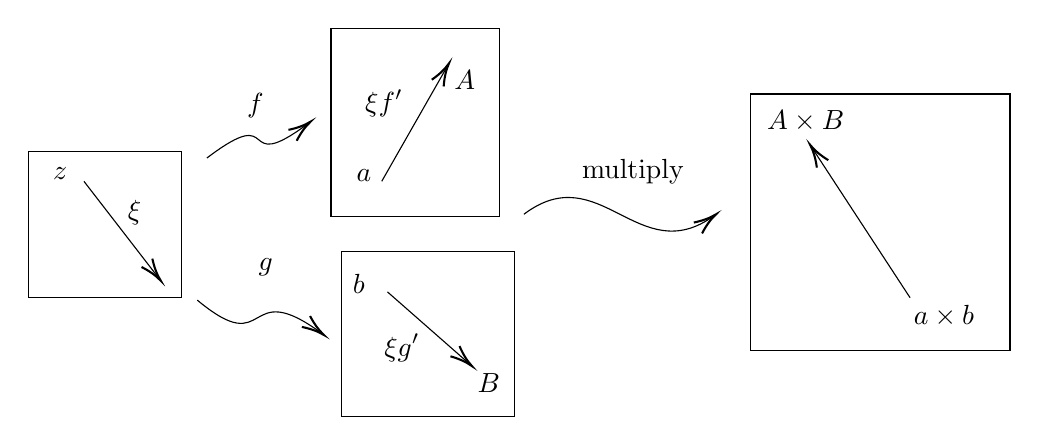
\begin{tikzpicture}[x=0.75pt,y=0.75pt,yscale=-1,xscale=1]
				%uncomment if require: \path (0,300); %set diagram left start at 0, and has height of 300
				
				%Straight Lines [id:da6920470629281815] 
				\draw    (97.84,112.88) -- (133.65,159.21) ;
				\draw [shift={(134.87,160.8)}, rotate = 232.31] [color={rgb, 255:red, 0; green, 0; blue, 0 }  ][line width=0.75]    (10.93,-3.29) .. controls (6.95,-1.4) and (3.31,-0.3) .. (0,0) .. controls (3.31,0.3) and (6.95,1.4) .. (10.93,3.29)   ;
				%Curve Lines [id:da3591348582207228] 
				\draw    (157.08,101.66) .. controls (193.74,73.89) and (170.52,111.41) .. (205.98,84.95) ;
				\draw [shift={(207.07,84.12)}, rotate = 502.85] [color={rgb, 255:red, 0; green, 0; blue, 0 }  ][line width=0.75]    (10.93,-3.29) .. controls (6.95,-1.4) and (3.31,-0.3) .. (0,0) .. controls (3.31,0.3) and (6.95,1.4) .. (10.93,3.29)   ;
				%Curve Lines [id:da20808412081192063] 
				\draw    (152.46,170.15) .. controls (188.19,199.77) and (174.04,157.91) .. (212.37,186.1) ;
				\draw [shift={(213.55,186.98)}, rotate = 216.93] [color={rgb, 255:red, 0; green, 0; blue, 0 }  ][line width=0.75]    (10.93,-3.29) .. controls (6.95,-1.4) and (3.31,-0.3) .. (0,0) .. controls (3.31,0.3) and (6.95,1.4) .. (10.93,3.29)   ;
				%Straight Lines [id:da33732657796359966] 
				\draw    (241.32,112.88) -- (272.72,57.81) ;
				\draw [shift={(273.71,56.07)}, rotate = 479.7] [color={rgb, 255:red, 0; green, 0; blue, 0 }  ][line width=0.75]    (10.93,-3.29) .. controls (6.95,-1.4) and (3.31,-0.3) .. (0,0) .. controls (3.31,0.3) and (6.95,1.4) .. (10.93,3.29)   ;
				%Straight Lines [id:da8094377499877842] 
				\draw    (244.09,166.17) -- (283.32,200.62) ;
				\draw [shift={(284.82,201.94)}, rotate = 221.29] [color={rgb, 255:red, 0; green, 0; blue, 0 }  ][line width=0.75]    (10.93,-3.29) .. controls (6.95,-1.4) and (3.31,-0.3) .. (0,0) .. controls (3.31,0.3) and (6.95,1.4) .. (10.93,3.29)   ;
				%Curve Lines [id:da5440688645875549] 
				\draw    (309.81,128.77) .. controls (346.47,101) and (364.98,155.71) .. (401.27,129.59) ;
				\draw [shift={(402.38,128.77)}, rotate = 502.85] [color={rgb, 255:red, 0; green, 0; blue, 0 }  ][line width=0.75]    (10.93,-3.29) .. controls (6.95,-1.4) and (3.31,-0.3) .. (0,0) .. controls (3.31,0.3) and (6.95,1.4) .. (10.93,3.29)   ;
				%Straight Lines [id:da5566338791478505] 
				\draw    (495.87,168.98) -- (448.83,97.02) ;
				\draw [shift={(447.73,95.34)}, rotate = 416.83000000000004] [color={rgb, 255:red, 0; green, 0; blue, 0 }  ][line width=0.75]    (10.93,-3.29) .. controls (6.95,-1.4) and (3.31,-0.3) .. (0,0) .. controls (3.31,0.3) and (6.95,1.4) .. (10.93,3.29)   ;
				%Shape: Rectangle [id:dp45889349804878155] 
				\draw   (71,98.72) -- (145.05,98.72) -- (145.05,168.98) -- (71,168.98) -- cycle ;
				%Shape: Rectangle [id:dp8202737570063776] 
				\draw   (216.89,39.13) -- (298.14,39.13) -- (298.14,129.82) -- (216.89,129.82) -- cycle ;
				%Shape: Rectangle [id:dp10318805190020353] 
				\draw   (221.88,146.54) -- (305.19,146.54) -- (305.19,226.25) -- (221.88,226.25) -- cycle ;
				%Shape: Rectangle [id:dp7465128179531455] 
				\draw   (419.04,70.8) -- (544,70.8) -- (544,194.46) -- (419.04,194.46) -- cycle ;
				
				% Text Node
				\draw (117.8,120.71) node [anchor=north west][inner sep=0.75pt]   [align=left] {$\displaystyle \xi $};
				% Text Node
				\draw (81.7,104.81) node [anchor=north west][inner sep=0.75pt]   [align=left] {$\displaystyle z$};
				% Text Node
				\draw (175.19,69.28) node [anchor=north west][inner sep=0.75pt]   [align=left] {$\displaystyle f$};
				% Text Node
				\draw (180.74,148.76) node [anchor=north west][inner sep=0.75pt]   [align=left] {$\displaystyle g$};
				% Text Node
				\draw (232.06,67.41) node [anchor=north west][inner sep=0.75pt]   [align=left] {$\displaystyle \xi f'$};
				% Text Node
				\draw (241.31,185.22) node [anchor=north west][inner sep=0.75pt]   [align=left] {$\displaystyle \xi g'$};
				% Text Node
				\draw (227.95,105.75) node [anchor=north west][inner sep=0.75pt]   [align=left] {$\displaystyle a$};
				% Text Node
				\draw (226.1,156.24) node [anchor=north west][inner sep=0.75pt]   [align=left] {$\displaystyle b$};
				% Text Node
				\draw (275.01,58.29) node [anchor=north west][inner sep=0.75pt]   [align=left] {$\displaystyle A$};
				% Text Node
				\draw (286.23,204.16) node [anchor=north west][inner sep=0.75pt]   [align=left] {$\displaystyle B$};
				% Text Node
				\draw (336.61,101.1) node [anchor=north west][inner sep=0.75pt]   [align=left] {multiply};
				% Text Node
				\draw (496.38,171.2) node [anchor=north west][inner sep=0.75pt]   [align=left] {$\displaystyle a\times b$};
				% Text Node
				\draw (425.77,77.7) node [anchor=north west][inner sep=0.75pt]   [align=left] {$\displaystyle A\times B$};
				
				
				\end{tikzpicture}
			\end{center}
			
			
		I'm not sure how to explain the Leibniz rule pure geometrically, so I will introduce a little algebra. As the picture above, $z$ is a complex number in $x-y$ plane, $\xi $ is a infinitesimal tangent vector from $z$. The images of these two point under $f,g$ are the second picture, the multiply of $f$ and $g$, we will obtain a new infinitesimal vector showed in the third picture. 
		
		So we have: 
			\begin{equation*}
			\begin{aligned}
				A&=a+\xi f', B=b+\xi g'\\
				\Rightarrow AB&=ab+\underbrace{\xi (f'b+ag')+\mathcal{O}(\xi ^2)}_{\text{image of }\xi}\\
				\Rightarrow (fg)'&=f'g+fg'
			\end{aligned}
			\end{equation*}
			
	\subsection{Exercise 4.30}
		As the dashed black path shows in the figure:
			\begin{equation*}
			\begin{aligned}
				\lim _{\Delta x \rightarrow 0} \frac{f(z+\Delta z)-f(z+\Delta y)}{ \Delta x}=\lim _{\Delta y \rightarrow 0} \frac{f(z+\Delta y)-f(z)}{\mi \Delta y}
			\end{aligned}
			\end{equation*}

			where the LHS leads to
				\begin{equation*}
				\begin{aligned}
					& \lim _{\Delta x \rightarrow 0} \frac{u(z+\Delta z)+\mi v(z+\Delta z)-u(z+\Delta y)-\mi v(z+\Delta y)}{ \Delta x} \\
					=& \lim _{\Delta x \rightarrow 0} \frac{u(z+\Delta z)-u(z+\Delta y)}{ \Delta x}+\lim _{\Delta x \rightarrow 0} \mi \frac{v(z+\Delta z)-v(z+\Delta y)}{\Delta x} \\
					=&\partial_{x} u+\mi \partial_{x} v
				\end{aligned}
				\end{equation*}
			
			and the RHS leads to
				\begin{equation*}
				\begin{aligned}
					&\lim _{\Delta y \rightarrow 0} \frac{u(z+\Delta y)+\mi v(z+\Delta y)-u(z)-\mi v(z)}{\mi \Delta y}\\
					=&\lim _{\Delta y \rightarrow 0} \frac{u(z+\Delta y)-u(z)}{\mi \Delta y}+\lim _{\Delta y \rightarrow 0} \frac{v(z+\Delta y)-v(z)}{\Delta y} \\
					=&-\mi \partial_{y} u+\partial_{y} v
				\end{aligned}
				\end{equation*}
			
			So we derive again:
				\begin{equation*}
				\begin{aligned}
					\begin{cases}
						&\pa_{x}u=\pa_{y}v\\
						&\pa_{y}u=-\pa_{x}v
					\end{cases}
				\end{aligned}
				\end{equation*}
			
	\subsection{Exercise 4.31*}
		This subject is pretty interesting. The analysis on quaternion is different, because the quaternion is non-commutative. We can have two kinds of differentiable:\textbf{ differnetiable on the left}:
			\begin{equation*}
				\lim_{h\rightarrow 0}[h^{-1}(f(q+h)-f(q))]
			\end{equation*}
			
		And \textbf{differentiable on the right}:
			\begin{equation*}
				\lim_{h\rightarrow 0}[(f(q+h)-f(q))h^{-1}]
			\end{equation*}
			
		The constraint on the anaylsis of quarternion is stronger, we have such theorem: The function $f$ defined and quaternion-differentiable on the left throughout a connected open set $U\subset \mathbb{H}$, then $f$ has the form:
			\begin{equation*}
			\begin{aligned}
				f(q)=a+qb,\text{for some a,b}\in\mathbb{H}
			\end{aligned}
			\end{equation*}
			
		Which means the functions of a quaternion variable which have quaternionic derivatives are just the constant and linear functions. 
		
		Besides differentiable, another standard for quaternion function is \textbf{regularity}. The holomorphic of quaternion function is defined on regularity. For a quaternion $q=t+\mi x+\mj y+\mk z$, we define the \textit{Left Cauchy-Riemann-Fueter operator} $\bar{\pa_l}$ as:
			\begin{equation*}
			\begin{aligned}
				\bar{\pa_l}\frac{\pa }{\pa t}+\mi \frac{\pa }{\pa x}+\mj \frac{\pa }{\pa y}+\mk \frac{\pa }{\pa z}
			\end{aligned}
			\end{equation*}
			
		Similarly,  the \textit{Right Cauchy-Riemann-Fueter operator} $\bar{\pa_r}$ is defined as:
			\begin{equation*}
			\begin{aligned}
				\bar{\pa_r}\frac{\pa }{\pa t}+\frac{\pa }{\pa x}\mi +\frac{\pa }{\pa y}\mj + \frac{\pa }{\pa z}\mk
			\end{aligned}
			\end{equation*}
		
		The \textit{Cullen differential operator} is defined:
			\begin{equation*}
			\begin{aligned}
				\pa_C=\frac{1}{2}\left(\frac{\pa }{\pa t}+\frac{\text{Im }(q)}{r}\frac{\pa }{\pa r}\right)
			\end{aligned}
			\end{equation*}
			
		The definition of regular funcions are as followed: A funtion $f:\mathbb{H}\rightarrow \mathbb{H}$ is \textbf{Left Regular in the sense of Fueter} at $q\in \mathbb{H}$ is $\bar{\pa_l}f(q)=0$, and is \textbf{Right Regular in the sense of Fueter} at $q\in \mathbb{H}$ is $f(q)\bar{\pa_r}=0$, is \textbf{Regular in sense of Cullen} if $\pa_Cf(q)=0$. 
		
		We will have Cauchy-Riemann-Fueter Equation, if we write $f(q)=g(v,w)+\mj h(v,w)$,  regular equals to :
			\begin{equation*}
			\begin{aligned}
				\begin{cases}
					\frac{\pa g}{\pa \bar{v}}=\frac{\pa h}{\pa \bar{w}}\\
					\frac{\pa g}{\pa w}=-\frac{\pa h}{\pa \bar{v}}
				\end{cases}
			\end{aligned}
			\end{equation*}
		
		For other property in quaternion, you can refer to the paper: \href{https://pdfs.semanticscholar.org/8988/92629ed7a9e1de8e1775641d76f4977c37ef.pdf?_ga=2.211757782.2104940488.1587127236-1682194610.1583117366}{A Survey on quaternionic analysis}.
		
	\subsection{Exercise 4.32}
%		We can set a circle as $z=r\me ^{\mi \theta}+z_0$, so the Mobius transformation transforms the circle as:
%			\begin{equation*}
%			\begin{aligned}
%				\begin{aligned}
%				\frac{a\left(r \me^{\mi \theta}+z_0\right)+b}{c\left(r \me^{\mi \theta}+z_0\right)+d} &=\frac{a r \me^{\mi \theta}+az_0+b}{c r \me^{\mi \theta}+c z_{0}+d} \\
%				&=\frac{b c-a d}{c^{2}} \frac{1}{r \me^{\mi \theta}+z_0+\frac{d}{c}}+\frac{a}{c} \\
%				&=\frac{b c-a d}{c^{2}} \frac{1}{r \me^{\mi \theta}+k}+\frac{a}{c} ,\text{ Where }k=z_0+\frac{d}{c}\\
%				&=\frac{b c-a d}{c^{2}} \frac{r \me^{\mi \theta}+k}{\left(r \me^{\mi \theta}+k\right)\left(r \me^{-\mi \theta}+k\right)}+\frac{a}{c} \\
%				&=\frac{b c-a d}{c^{2}} \frac{r \me^{\mi \theta}+k}{r^{2}+k^{2}+r k\left(\me^{-b}+\me^{-\mi \theta}\right)}+\frac{a}{c} \\
%				&=\frac{b c-a d}{c^{2}} \frac{r \me^{-\mi \theta}+k}{r^{2}+k^{2}+2 r k \cos \theta}+\frac{a}{c} \\
%				&=\frac{(b c-a d) r}{c^{2}\left(r^{2}+k^{2}+2 r k \cos \theta\right)} \me^{-\mi\theta}+\frac{(b c-a d) k}{c^{2}\left(r^{2}+k^{2}+2 r k \cos \theta\right)}+\frac{a}{c}
%				\end{aligned}
%			\end{aligned}
%			\end{equation*}
%		
%		So the Mobius transformation transforms a circle to a circle, but changes the 
		
		This one is pretty interesting, the key to this problem is that the inversion maps a circle to a circle. If you write the circle as $z=r\me^{\mi \theta}+z_0$, things may get mess and tough(as I did in the first time). We should use the Cartesian coordinate. Set $z=x+\mi y, \frac{1}{z}=u+\mi v$, we will get:
			\begin{equation*}
			\begin{aligned}
				z=\frac{u}{u^2+v^2}&-\mi \frac{v}{u^2+v^2}=x+\mi y\\
				\Rightarrow x^2+y^2&=\frac{1}{u^2+v^2}
			\end{aligned}
			\end{equation*}
			
		Because $z$ is a circle or a line, we have:
			\begin{equation*}
			\begin{aligned}
				&A(x^2+y^2)+Bx+Cy+D=0\\
				\Rightarrow &A(\frac{1}{u^2+v^2})+B\frac{u}{u^2+v^2}-C\frac{v}{u^2+v^2}+D=0\\
				\Rightarrow &D(u^2+v^2)+Bu-Cv+A=0
			\end{aligned}
			\end{equation*}
			
		Which means $\frac{1}{z}=u+\mi v$ is a circle or a line. Other steps of Mobius transformation obviously maps circles to a cirlce, which means the whole transformation maps a circle to a circle. 
		
		From the formular above, we can see the radius of the circle is mapped as:
			\begin{equation*}
			\begin{aligned}
				r^2=\frac{1}{4A^2}\left(B^2+C^2-4AD\right)\rightarrow \frac{1}{4D^2}\left(B^2+C^2-4AD\right)=\frac{A^2}{D^2}r^2
			\end{aligned}
			\end{equation*}
			
		The center of the circle is mapped as:
			\begin{equation*}
			\begin{aligned}
				\left(-\frac{B}{2A},-\frac{C}{2A}\right)\rightarrow\left(-\frac{B}{2D},\frac{C}{2D}\right)
			\end{aligned}
			\end{equation*}
		
		If we use polar coordinate, we will find that for a circle:$z=r\me^{\mi \theta}+a+\mi b$, the radius $r$ is mapped into:
			\begin{equation*}
			\begin{aligned}
				r\rightarrow \frac{r}{|a^2+b^2-r^2|}
			\end{aligned}
			\end{equation*}
			
		We can use the language of the complex number to restate this conclusion. In the complex plane, the circle of radius $r$ around the point $a$ is expressed as: 
			\begin{equation*}
				(z-a)(z-a)^{*}=r^{2}
			\end{equation*}
			
		We define $w=\frac{1}{z}$, and we can calculate that for $a a^{*} \neq r^{2}$, the result for $w$ is
			\begin{equation*}
			\begin{aligned}
				&w w^{*}-\frac{a w+a^{*} w^*}{\left(a^{*} a-r^{2}\right)}+\frac{a a^{*}}{\left(a a^{*}-r^{2}\right)^{2}}=\frac{r^{2}}{\left(a a^{*}-r^{2}\right)^{2}} \\
				\Rightarrow&\left(w-\frac{a^{*}}{a a^{*}-r^{2}}\right)\left(w^*-\frac{a}{a^{*} a-r^{2}}\right)=\left(\frac{r}{\left|a a^{*}-r^{2}\right|}\right)^{2}
			\end{aligned}
			\end{equation*}
		
		showing that the $w$ describes the circle of center $\frac{a^*}{\left(a a^*-r^{2}\right)}$ and radius $\frac{r}{\left|a^{*} a-r^{2}\right|}$.
		When $a^{*} a \rightarrow r^{2}$, the equation for $w$ becomes:
			\begin{equation*}
			\begin{aligned}
				& a w+a^{*} w^{*}=1 \\
				\Rightarrow &2 \operatorname{Re}(aw)=1 \\
				\Rightarrow &\operatorname{Re}(a) \operatorname{Re}(w)-\operatorname{Im}(a) \operatorname{Im}(w)=\frac{1}{2} \\
				\Rightarrow &\operatorname{Im}(w) =\frac{\operatorname{Re}(a)}{\operatorname{Im}(a)} \cdot \operatorname{Re}(w)-\frac{1}{2 \cdot \operatorname{Im}(a)}
			\end{aligned}
			\end{equation*}
		
		Which means when $a^{*} a \rightarrow r^{2}$, the Mobius transformation maps a circle to a line. In fact, a line in the complex plane can be described as :
			\begin{equation*}
			\begin{aligned}
				zz_0+\overline{zz_0}=D
			\end{aligned}
			\end{equation*}
		
		Can you show why?
		
		The third step is a dilation. If we set a circle as $z=\rho+r\me^{\mi \theta}$, we want to find the result of a constant complex number $m=a+\mi b$ multiplies on the circle:
			\begin{equation*}
			\begin{aligned}
				z \cdot m &=\rho \cdot m+r \cdot m \me^{\mi \theta} \\
				&=\rho \cdot m+r(a+\mi b)(\cos \theta+\mi \sin \theta) \\
				&=\rho \cdot m+r(a\cos\theta-b \sin \theta+\mi a\sin \theta+\mi b \cos \theta) \\
				&=\rho \cdot m+r \sqrt{a^{2}+b^{2}}[\cos (\theta+\varphi)+\mi \sin (\theta+\varphi)] \\
				&=\rho \cdot m+r \sqrt{a^{2}+b^{2}} \me^{\mi(\theta+\varphi)}
			\end{aligned}
			\end{equation*}
			
		Which means this maps the center as:
			\begin{equation*}
			\begin{aligned}
				\rho\mapsto \rho\cdot m
			\end{aligned}
			\end{equation*}
		
		Maps the radius to:
			\begin{equation*}
			\begin{aligned}
				r\mapsto r|m|=r\sqrt{a^{2}+b^{2}}
			\end{aligned}
			\end{equation*}
		
		And this map add a phase to the circle. 
		
		So, in all, the Mobius changes the circle with radius $r$ and center $p$ to another circle:
			\begin{equation*}
			\begin{aligned}
				r&\mapsto r\left|\frac{\frac{bc-ad}{c^2}}{|p+\frac{d}{c}|^2-r^2}\right|=r\left|\frac{|c|(bc-ad)}{c^2|pc+d|^2-c^2|c|r^2}\right|\\
				p&\mapsto \frac{bc-ad}{c^2}\frac{\left(p+\frac{d}{c}\right)^*}{|p+\frac{d}{c}|^2-r^2}+\frac{a}{c}
			\end{aligned}
			\end{equation*}
	\subsection{Exercise 4.33}
		My intuitive proof is written as follows. Think that how can we describe the perpendicular bisector of two points, $b,d$? Of course, the kindergarten maths tells us the distance between every point on the line and $b$ and $d$ are equal, which means, if $z$ is on the line, we have the equation of the line as:
			\begin{equation*}
			\begin{aligned}
				|z-b|=|z-d|
			\end{aligned}
			\end{equation*}
			
		If we rearrange the equation, we will get:
			\begin{equation*}
			\begin{aligned}
				\frac{|z-b|}{|z-d|}=1
			\end{aligned}
			\end{equation*}
			
		Which means the map $M(z)=\frac{z-b}{z-d}$ maps $z$ to a number $M(z)$, at the same time, $|M(z)|=1$, which means this maps $z$ to a unit circle. Here we finish the proof.
		
		To solve the speed, we need to parametrize the perpendicular bisector $L$ by:
		\begin{equation*}
		\begin{aligned}
		z=\frac{b+d}{2}+\mi (d-b)at,\quad a,t\in R
		\end{aligned}
		\end{equation*}
		
		Where $t$ is the time parameter(This parametrization is done by add a perpendicular vector to the middle point of $bd$). And the speed of the point $z$ is :
			\begin{equation*}
			\begin{aligned}
				v=\frac{\di }{\di t}\left|z-\frac{b+d}{2}\right|=|a(d-b)|
			\end{aligned}
			\end{equation*}
		
		The Mobius transformation transforms $z$ to:
			\begin{equation*}
			\begin{aligned}
				M(z)=\frac{z-b}{z-d}=\frac{(d-b)/2+\mi (d-b)at}{(b-d)/2+\mi (d-b)at}=\frac{1+2\mi at}{-1+2\mi at}=\frac{4a^2t^2-1}{4a^2t^2+1}-\mi \frac{4at}{4a^2t^2+1}
			\end{aligned}
			\end{equation*}
		
		As $at\in \mathbb{R}$, we have:
			\begin{equation*}
			\begin{aligned}
				M(z)=\me ^{\mi \theta(t)}
			\end{aligned}
			\end{equation*}
		where
			\begin{equation*}
			\tan \theta(t)=-\frac{4 a t}{4 a^{2} t^{2}-1}, \cos \theta=\frac{4 a^{2} t^{2}-1}{\sqrt{\left(4 a^{2} t^{2}-1\right)^{2}+16 a^{2} t^{2}}}=\frac{4 a^{2} t^{2}-1}{4 a^{2} t^{2}+1}
			\end{equation*}
		
		Therefore:
			\begin{equation*}
			\begin{aligned}
			\dot{\theta}(t) \sec ^{2} \theta(t)=-\frac{\mathrm{d}}{\mathrm{d} t} \frac{4 a t}{4 a^{2} t^{2}-1}=\frac{4 a\left(1+4 a^{2} t^{2}\right)}{\left(1-4 a^{2} t^{2}\right)^{2}}
			\end{aligned}
			\end{equation*}
		
		Thus the motion on the unit circle is described by the angular velocity
			\begin{equation*}
			\begin{aligned}
				\omega(t)=\dot{\theta}(t)=\cos ^{2} \theta(t) \frac{4 a\left(1+4 a^{2} t^{2}\right)}{\left(1-4 a^{2} t^{2}\right)^{2}}=\frac{4 a}{1+4 a^{2} t^{2}}
			\end{aligned}
			\end{equation*}
		
		The relationship between angular velocity and time is plotted below:
			\begin{center}
				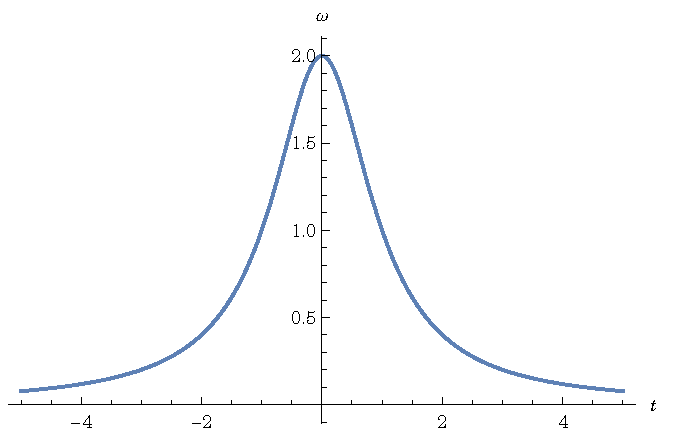
\includegraphics[scale=1]{velocity-of-the-point.pdf}
			\end{center}
		
		We see that the angular velocity of $M(z)$ takes the maximum value $4 a /\left(1+4 a^{2}\right)$ when the point $z$ is passing through the point $(b+d) / 2 .$ Noting that the integration:
			\begin{equation*}
			\int_{-\infty}^{\infty} \omega(t) \mathrm{d} t=\left.4 a \cdot \frac{\arctan (2 a t)}{2 a}\right|_{-\infty} ^{\infty}=2 \pi
			\end{equation*}

		which is independent of the value of $a$ and is in agreement with the fact that $M(z)$ is a bijection. (This
		result also means that our result is correct.)
		
		The inverse speed of the line is also simple. Suppose the angular speed of the point on the unit circle is  $\omega$, we can write the point as:
			\begin{equation*}
			\begin{aligned}
				M(z)=\me^{\mi \omega t}=\frac{z-b}{z-d}
			\end{aligned}
			\end{equation*}
		
		We can rewrite the equation as:
			\begin{equation*}
			\begin{aligned}
				z=\frac{d\me^{\mi \omega t}-b}{\me^{\mi \omega t}-1}
			\end{aligned}
			\end{equation*}
		
		If we want to figure out the speed on the line, just figure out the distance between our point and the middle point of $bd$, which means:
			\begin{equation*}
			\begin{aligned}
				s&=|z-\frac{b+d}{2}|\\
				&=|\frac{d-b}{2}\frac{\me^{\mi \omega t}+1}{\me^{\mi \omega t}-1}|\\
				&=|-\mi \frac{d-b}{2}\cot\left(\frac{\omega t}{2}\right)|\\
				&=\frac{|d-b|}{2}|\cot\left(\frac{\omega t}{2}\right)|
			\end{aligned}
			\end{equation*}
		
		So the speed on the line can be written as:
			\begin{equation*}
			\begin{aligned}
				v=\frac{\di s}{\di t}=\frac{|d-b|}{2}|\frac{\omega}{\cos\omega t-1}|
			\end{aligned}
			\end{equation*}
			
	\subsection{Exercise 4.34}
		\subsubsection{}
			We have:
				\begin{equation*}
				\begin{aligned}
					M(z)&=\frac{z-a}{a^*z-1}\\
					\Rightarrow M(M(z))&=\frac{\frac{z-a}{a^*z-1}-a}{a^*\frac{z-a}{a^*z-1}-1}=\frac{z(1-aa^*)}{1-aa^*}=z
				\end{aligned}
				\end{equation*}
		
		\subsubsection{}
			If you figure out what the image of this map is, things  may get tough. We should tear the Mobius transformation into 4 part. We set the center of the circle as $p$:
				\begin{enumerate}
					\item $z\rightarrow z+\frac{d}{c}=z-\frac{1}{a^*}$\\
					$r=1\mapsto 1, p=0\mapsto -\frac{1}{a^*}$
					\item $z\rightarrow \frac{1}{z}$\\
					$r=1\mapsto \frac{1}{|\frac{1}{|a|^2}-1|}=\frac{|a|^2}{1-|a|^2},p=-\frac{1}{a^*}\mapsto \frac{a^*}{|a|^2-1}$
					\item $z\rightarrow \frac{bc-ad}{c^2}z=\frac{1-|a|^2}{a^{*^2}}z$\\
					$r=\frac{|a|^2}{|1-|a|^2|}\mapsto \frac{|a|^2}{|1-|a|^2|}\times \frac{|1-|a|^2|}{|a|^2}=1, p=\frac{a^*}{|a|^2-1}\times \frac{1-|a|^2}{a^{*^2}}z=-\frac{1}{a^*}$
					\item $z\rightarrow  z+\frac{a}{c}=z+\frac{1}{a^*}$\\
					$r=1\mapsto 1,p=-\frac{1}{a^*}+\frac{1}{a^*}=0$
				\end{enumerate}
			
			Here we can see that this map will finally map a unit circle to a unit circle. We use the conclusion that the image of the radius and center of the Mobius transformation which we proved in Exercise 4.32. 
			
			You can also compute the module directly:
				\begin{equation*}
				\begin{aligned}
					&\left|\frac{z-a}{a^{*} z-1}\right|^{2} \\
					=&\left|\frac{z-a}{a^{*} z-1}\right|\left|\frac{z^{*}-a^{*}}{a z^{*}-1}\right| \\
					=&\left|\frac{|z|^{2}+|a|^{2}-z a^{*}-a z^{*}}{|a|^{2}|z|^{2}-a^{*} z-z^{*} a+1}\right| \\
					=&\left|\frac{1+|a|^{2}-z a^{*}-a z^{*}}{|a|^{2}-a^{*} z-z^{*} a+1}\right| \\
					=&1
				\end{aligned}
				\end{equation*}
		
		\subsubsection{}
			We first prove that $|a^*z-1|^2-|z-a|^2=(1-|a|^2)(1-|z|^2)$.
				\begin{equation*}
				\begin{aligned}
					\text{RHS}&=(a^*z-1)(az^*-1)-(z-a)(z^*-a^*)\\
					&=|a|^2|z|^2-a^*z-az^*+1-|z|^2+za^*+az^*-|a|^2\\
					&=1-|z|^2-|a|^2-|a|^2|z|^2\\
					\text{LHS}&=(1-|a|^2)(1-|z|^2)\\
					&=1-|z|^2-|a|^2-|a|^2|z|^2\\
					\Rightarrow &\text{RHS}=\text{LHS}
				\end{aligned}
				\end{equation*}
			
			If $a$ is inside the disk, which means:
				\begin{equation*}
				\begin{aligned}
					&|a|<1\\
					\Rightarrow &\underbrace{(1-|a|^2)}_{>0}\underbrace{(1-|z|^2)}_{>0}>0\\
					\Rightarrow &|a^*z-1|^2-|z-a|^2>0\\
					\Rightarrow &\left|\frac{z-a}{a^*z-1}\right|<1
				\end{aligned}
				\end{equation*}
			
			Which means $ M(z) $ maps the unit disc to itself. For $a$ does  not lie inside the disc, we have:
				\begin{equation*}
				\begin{aligned}
					\left|\frac{z-a}{a^*z-1}\right|>1
				\end{aligned}
				\end{equation*}
			
			Which means it maps the unit disc out of the disc. 
	
	\subsection{Exercise 4.35}
		We shall first figure out the meaning of "point symmetric with respect to a circle". 
		
		 In the plane, the inverse of a point $ P $ with respect to a reference circle with center $ O $ and radius $ r $ is a point $ P' $, lying on the \textbf{ray} from $ O $ through $ P  $ such that
		 	\begin{equation*}
		 	\begin{aligned}
		 		OP\cdot OP^{\prime }=r^{2}
		 	\end{aligned}
		 	\end{equation*}
			\begin{center}
				\tikzset{every picture/.style={line width=0.75pt}} %set default line width to 0.75pt        
				
				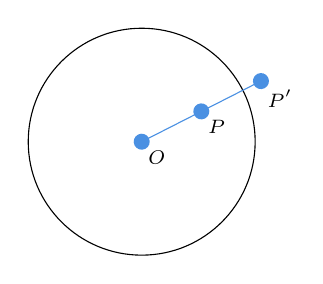
\begin{tikzpicture}[x=0.75pt,y=0.75pt,yscale=-1,xscale=1]
				%uncomment if require: \path (0,300); %set diagram left start at 0, and has height of 300
				
				%Shape: Circle [id:dp7397711329536104] 
				\draw   (158.21,155.13) .. controls (158.21,124.93) and (182.68,100.46) .. (212.88,100.46) .. controls (243.07,100.46) and (267.54,124.93) .. (267.54,155.13) .. controls (267.54,185.32) and (243.07,209.79) .. (212.88,209.79) .. controls (182.68,209.79) and (158.21,185.32) .. (158.21,155.13) -- cycle ;
				%Straight Lines [id:da2744213172174935] 
				\draw [color={rgb, 255:red, 74; green, 144; blue, 226 }  ,draw opacity=1 ]   (270.33,125.92) -- (212.88,155.13) ;
				\draw [shift={(212.88,155.13)}, rotate = 153.05] [color={rgb, 255:red, 74; green, 144; blue, 226 }  ,draw opacity=1 ][fill={rgb, 255:red, 74; green, 144; blue, 226 }  ,fill opacity=1 ][line width=0.75]      (0, 0) circle [x radius= 3.35, y radius= 3.35]   ;
				\draw [shift={(241.6,140.52)}, rotate = 153.05] [color={rgb, 255:red, 74; green, 144; blue, 226 }  ,draw opacity=1 ][fill={rgb, 255:red, 74; green, 144; blue, 226 }  ,fill opacity=1 ][line width=0.75]      (0, 0) circle [x radius= 3.35, y radius= 3.35]   ;
				\draw [shift={(270.33,125.92)}, rotate = 153.05] [color={rgb, 255:red, 74; green, 144; blue, 226 }  ,draw opacity=1 ][fill={rgb, 255:red, 74; green, 144; blue, 226 }  ,fill opacity=1 ][line width=0.75]      (0, 0) circle [x radius= 3.35, y radius= 3.35]   ;
				
				% Text Node
				\draw (214.55,158.41) node [anchor=north west][inner sep=0.75pt]  [font=\scriptsize,rotate=-357.88] [align=left] {$\displaystyle O$};
				% Text Node
				\draw (243.6,143.52) node [anchor=north west][inner sep=0.75pt]  [font=\scriptsize] [align=left] {$\displaystyle P$};
				% Text Node
				\draw (272.33,128.92) node [anchor=north west][inner sep=0.75pt]  [font=\scriptsize] [align=left] {$\displaystyle P'$};
				
				
				\end{tikzpicture}
				
			\end{center}
			
		This is called circle inversion or plane inversion. To see the invariant, we also tear the Mobius transformation into 4 parts. Suppose the radius of the circle is $R$, the coordinate of the center, point$P,P'$ are $m,p,q$,we have:
			\begin{enumerate}
				\item $z\rightarrow z+\frac{d}{c}$ The translation keeps the symmetry trivially. 
				\item $z\rightarrow \frac{1}{z}$\\
				 We have $ |p-m||q-m|= |p-m|\lambda|p-m|=R^2 $(because $p,q$ are on the same ray)\\
				 	\begin{equation*}
				 	\begin{aligned}
				 		\Rightarrow& (p-m)(q-m)^*=R^2\\
				 		\Rightarrow& p q^{*}+|m|^{2}-p m^{*}-q^{*} m=R^{2} \\
				 		\Rightarrow& p q^{*}-p m^{*}-q^{*} m=R^{2}-|m|^{2} \\
				 		\Rightarrow& 1-\frac{m^{*}}{q^{*}}-\frac{m}{p}=-\frac{|m|^{2}-R^{2}}{p q^{*}} \\
				 		\Rightarrow& \frac{m m^{*}-R^{2} }{\left(|m|^{2}-R^{2}\right)^{2}}-\frac{1}{q^{*}} \frac{m^{*}}{|m|^{2}-R^{2}}-\frac{1}{p} \frac{m}{|m|^{2}-R^{2}}=-\frac{1}{p q^{*}} \\
				 		\Rightarrow& \frac{m m^{*}}{\left(|m|^{2}-R^{2}\right)^{2}}-\frac{1}{q^{*}} \frac{m^{*}}{|m|^{2}-R^{2}}-\frac{1}{p} \frac{m}{|m|^{2}-R^{2}}+\frac{1}{p q}=\frac{R^{2}}{\left(|m|^{2}-R^{2}\right)^{2}} \\
				 		\Rightarrow& \left(\frac{1}{p}-\frac{m^{*}}{|m|^{2}-R^{2}}\right)\left(\frac{1}{q}-\frac{m^{*}}{| m|^{2}-R^{2}}\right)^{*}=\frac{R^{2}}{\left(|m|^{2}-R^{2}\right)^{2}}
				 	\end{aligned}
				 	\end{equation*}
				 	
				 	We see $\frac{1}{q}$ and $\frac{1}{p}$ are symmetry with respect to the transformed circle.  
				 	
				\item $z\rightarrow \frac{bc-ad}{c^2}z$ is an amplitwist. \\
				In this situation, these two point can be set as: 
					\begin{equation*}
						p=m+r\me^{\mi \theta},q=m+\frac{R^2}{r}\me^{\mi \theta}
					\end{equation*}
				
				After the amplitwist(multiplied by $a$), the points are transformed to :
					\begin{equation*}
					\begin{aligned}
						p'=ma+r|a|\me^{\mi (\theta+\varphi)},q'=ma+|a|\frac{R^2}{r}\me^{\mi (\theta+\varphi)}
					\end{aligned}
					\end{equation*}
					
				It agreed with the transformed circle that we showed in Exercise 4.32. So it is invariant. 
				\item $z\rightarrow  z+\frac{a}{c}$ This is also an translation. 
			\end{enumerate}
		
		So after four steps, the symmetry is invariant.
			\subsubsection{More information}
			Interestingly, the stereographic projection is such an inversion. It is the inversion of a sphere. 
				\begin{center}
					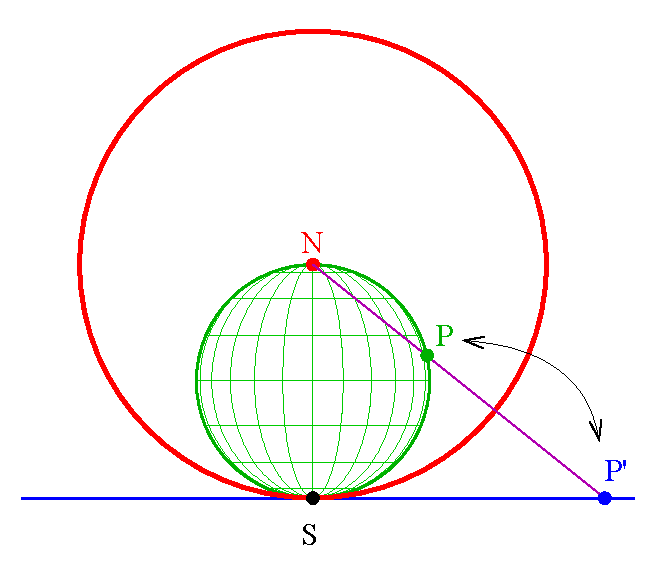
\includegraphics[width=2in, keepaspectratio]{pdfresizer-com-pdf-crop.pdf}
				\end{center}
			
			We will see it later. Higer dimensional inversion looks like this, it is an inversion of a hyperboloid of one sheet:
				\begin{center}
					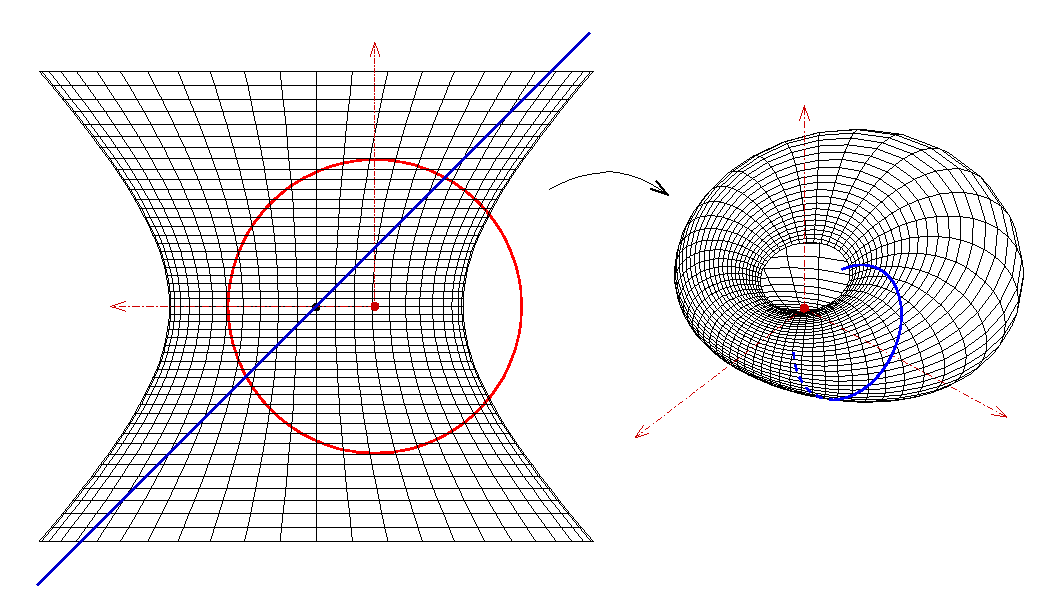
\includegraphics[width=3in, keepaspectratio]{hyperinversion.pdf}
				\end{center}
			
	\subsection{Exercise 4.36}
		We can also show that the cross-ratio is invariant from step to step. 
			\begin{enumerate}
				\item $z\rightarrow z+\frac{d}{c}$ The translation keeps the cross ratio trivially. 
				\item $z\rightarrow \frac{1}{z}$ The inversion truns cross ratio into:
					\begin{equation*}
					\begin{aligned}
						\frac{(z_1-z_3)(z_2-z_4)}{(z_2-z_3)(z_1-z_4)}\mapsto & \frac{\left(\frac{1}{z_1}-\frac{1}{z_3}\right)\left(\frac{1}{z_2}-\frac{1}{z_4}\right)}{\left(\frac{1}{z_2}-\frac{1}{z_3}\right)\left(\frac{1}{z_1}-\frac{1}{z_4}\right)}\\
						=&\frac{\frac{(z_3-z_1)(z_4-z_2)}{z_1z_3z_2z_4}}{\frac{(z_3-z_2)(z_4-z_1)}{z_2z_3z_1z_4}}\\
						=&\frac{(z_1-z_3)(z_2-z_4)}{(z_2-z_3)(z_1-z_4)}
					\end{aligned}
					\end{equation*}
				\item $z\rightarrow az$ This turns the cross ratio into:
					\begin{equation*}
					\begin{aligned}
						\frac{(z_1-z_3)(z_2-z_4)}{(z_2-z_3)(z_1-z_4)}\mapsto &\frac{(az_1-az_3)(az_2-az_4)}{(az_2-az_3)(az_1-az_4)}=\frac{(z_1-z_3)(z_2-z_4)}{(z_2-z_3)(z_1-z_4)}
					\end{aligned}
					\end{equation*}
				\item This translation is also trivial. 
			\end{enumerate}
		
		So the Mobius transformation keeps the cross ratio. 
			
			\subsubsection{More information}
				The cross ratio have some geometrical meaning. We denote a cross ratio by:
					\begin{equation*}
					\begin{aligned}
						(z_1,z_2;z_3,z_4)=\frac{(z_1-z_3)(z_2-z_4)}{(z_2-z_3)(z_1-z_4)}
					\end{aligned}
					\end{equation*}
					
				The cross ratio is invariant in this situation:
				\begin{center}
					\tikzset{every picture/.style={line width=0.75pt}} %set default line width to 0.75pt        
					
					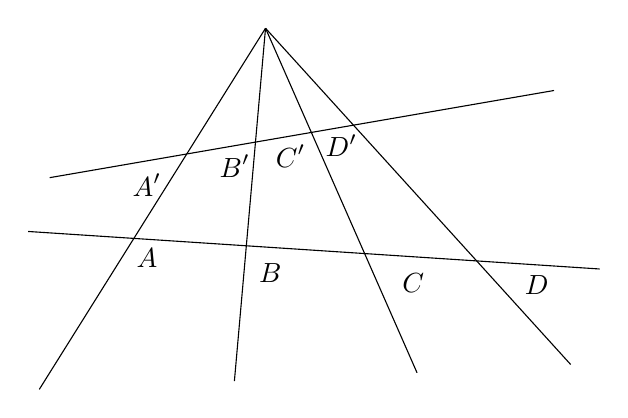
\begin{tikzpicture}[x=0.75pt,y=0.75pt,yscale=-1,xscale=1]
					%uncomment if require: \path (0,300); %set diagram left start at 0, and has height of 300
					
					%Straight Lines [id:da9566018255817191] 
					\draw    (284.33,80.08) -- (175.33,254.08) ;
					%Straight Lines [id:da9459843750529865] 
					\draw    (284.33,80.08) -- (431.33,242.08) ;
					%Straight Lines [id:da18961598379924305] 
					\draw    (284.33,80.08) -- (357.33,246.08) ;
					%Straight Lines [id:da04469468587499037] 
					\draw    (284.33,80.08) -- (269.33,250.08) ;
					%Straight Lines [id:da6192364498188526] 
					\draw    (170,178) -- (445.33,196.08) ;
					%Straight Lines [id:da7645860235219003] 
					\draw    (180.33,152.08) -- (423.33,110.08) ;
					
					% Text Node
					\draw (221,185) node [anchor=north west][inner sep=0.75pt]   [align=left] {$\displaystyle A$};
					% Text Node
					\draw (280,192) node [anchor=north west][inner sep=0.75pt]   [align=left] {$\displaystyle B$};
					% Text Node
					\draw (349,197) node [anchor=north west][inner sep=0.75pt]   [align=left] {$\displaystyle C$};
					% Text Node
					\draw (408,198) node [anchor=north west][inner sep=0.75pt]   [align=left] {$\displaystyle D$};
					% Text Node
					\draw (219,149) node [anchor=north west][inner sep=0.75pt]   [align=left] {$\displaystyle A'$};
					% Text Node
					\draw (261,140) node [anchor=north west][inner sep=0.75pt]   [align=left] {$\displaystyle B'$};
					% Text Node
					\draw (288,135) node [anchor=north west][inner sep=0.75pt]   [align=left] {$\displaystyle C'$};
					% Text Node
					\draw (312,130) node [anchor=north west][inner sep=0.75pt]   [align=left] {$\displaystyle D'$};
					
					
					\end{tikzpicture}
				\end{center}
				
				\begin{equation*}
				\begin{aligned}
					(A,B;C,D)&=\frac{AC\cdot BD}{BC\cdot AD}\\
					(A,B;C,D)&=(A',B';C'D')
				\end{aligned}
				\end{equation*}
			
			We see that the points $A,B,C,D$ and $A',B',C',D'$ are linked with the cross ratio. 
			
			Inerestingly, we have met the cross ratio far earlier, you are just unaware of it. If we rearrange the input in the cross ratio, we will get 6 different values:
				\begin{equation*}
				\begin{aligned}
					&(A, B ; C, D)=(B, A ; D, C)=(C, D ; A, B)=(D, C ; B, A)=\lambda\\
					&(A, B ; D, C)=(B, A ; C, D)=(C, D ; B, A)=(D, C ; A, B)=\frac{1}{\lambda}\\
					&(A, C ; B, D)=(B, D ; A, C)=(C, A ; D, B)=(D, B ; C, A)=1-\lambda\\
					&(A, C ; D, B)=(B, D ; C, A)=(C, A ; B, D)=(D, B ; A, C)=\frac{1}{1-\lambda}\\
					&(A, D ; B, C)=(B, C ; A, D)=(C, B ; D, A)=(D, A ; C, B)=\frac{\lambda-1}{\lambda}\\
					&(A, D ; C, B)=(B, C ; D, A)=(C, B ; A, D)=(D, A ; B, C)=\frac{\lambda}{\lambda-1}
				\end{aligned}
				\end{equation*}
			
			Do you feel familiar? We have found it in Exercise 1.7, it is just the group $S_3$. There's another group lies in the equations above, can you see it? If we try to find out what permutation keeps the cross ratio invariant, we can see:
				\begin{equation*}
				\begin{aligned}
					(A, B ; C, D)=(B, A ; D, C)=(C, D ; A, B)=(D, C ; B, A)
				\end{aligned}
				\end{equation*}
			
			Which means the permutation:
				\begin{equation*}
				\begin{aligned}
					I, (12)(34),(13)(24),(14)(23)
				\end{aligned}
				\end{equation*}
			
			Keeps the cross ratio invariant. By $(12)(34)$, we mean we exchange the position between the first and the second element, and exchange the position between the third and the fourth element. Do you see what group it is? It is just $Z_2\times Z_2$, the Vierergruppe. 
			
			The appearance of two groups is not a coincidence. Set the full permuataton of the cross ratio as a group, namely $S_4$(there are 4!=24 elements in the group). In the language of group theory, the symmetric group $\mathrm{S}_{4}$ acts on the cross ratio by permuting coordinates. The \textbf{kernel} of this action is isomorphic to the Klein four-group $Z_2\times Z_2$.  The \textbf{effective} symmetry group is isomorphic to  $S_{3}$ , which means:
				\begin{equation*}
				\begin{aligned}
					S_4/Z_2\times Z_2=S_3
				\end{aligned}
				\end{equation*}
			
			There is also a projective group lies in the cross ratio, we will find it later. 
			
			Now let's consider what if there is one point approaches to infinity. If one point of $z_2,z_3,z_4$ approaches to infinity, we have:
				\begin{equation*}
				\begin{aligned}
					(z_1,z_2;z3,z4)=\frac{z_1-z_3}{z_1-z_4},\frac{z_2-z_4}{z-z_4},\text{ or }\frac{z-z_3}{z_2-z_3}
				\end{aligned}
				\end{equation*}
	
	\subsection{Exercise 4.37}
		First, if four points lie on a line, we have: 
			\begin{equation*}
			\begin{aligned}
				\frac{(z_1-z_3)(z_2-z_4)}{(z_2-z_3)(z_1-z_4)}=\frac{(z_1-z_3)\lambda_{1}(z_1-z_3)}{\lambda_{2}(z_1-z_3)\lambda_{3}(z_1-z_3)}=\frac{\lambda_{1}}{\lambda_{2}\lambda_{3}}\in \mathbb{R}
			\end{aligned}
			\end{equation*}
			
		If the four points lies on a circle, we have:
			\begin{equation*}
			\begin{aligned}
				&\frac{(z_1-z_3)(z_2-z_4)}{(z_2-z_3)(z_1-z_4)}\\
				=&\frac{(r\me^{\mi\varphi_1}+m-r\me^{\mi\varphi_3}-m)(r\me^{\mi\varphi_2}+m-r\me^{\mi\varphi_4}-m)}{(r\me^{\mi\varphi_2}+m-r\me^{\mi\varphi_3}-m)(r\me^{\mi\varphi_1}+m-r\me^{\mi\varphi_4}-m)}\\
				=&\frac{(\me^{\mi\varphi_1}-\me^{\mi\varphi_3})(\me^{\mi\varphi_2}-\me^{\mi\varphi_4})}{(\me^{\mi\varphi_2}-\me^{\mi\varphi_3})(\me^{\mi\varphi_1}-\me^{\mi\varphi_4})}\\
				=&\frac{\cos \left(\frac{\varphi_1}{2}+\frac{\varphi_2}{2}-\frac{\varphi_3}{2}-\frac{\varphi_4}{2}\right)-\cos \left(\frac{\varphi_1}{2}-\frac{\varphi_2}{2}-\frac{\varphi_3}{2}+\frac{\varphi_4}{2}\right)}{\cos \left(\frac{\varphi_1}{2}+\frac{\varphi_2}{2}-\frac{\varphi_3}{2}-\frac{\varphi_4}{2}\right)-\cos \left(\frac{\varphi_1}{2}-\frac{\varphi_2}{2}+\frac{\varphi_3}{2}-\frac{\varphi_4}{2}\right)}\\
				=&\csc\left(\frac{\varphi_2-\varphi_3}{2}\right)\csc\left(\frac{\varphi_1-\varphi_4}{2}\right)\sin\left(\frac{\varphi_1-\varphi_3}{2}\right)\sin\left(\frac{\varphi_2-\varphi_4}{2}\right)\in \mathbb{R}
			\end{aligned}
			\end{equation*}
			
			For a simplier proof, we notice that:
				\begin{equation*}
				\begin{aligned}
					\arg(z_1,z_2;z_3,z_4)=\arg\frac{z_1-z_3}{z_1-z_4}-\arg\frac{z_2-z_3}{z_2-z_4}
				\end{aligned}
				\end{equation*}
				
			If these points lie on a same circle or line, the angle equals to $0,\pm \pi$. 
			
			What about the inverse? How can we compute the cross ratio of any four points? We know that for any three points, they are on a circle, say $z_2,z_3,z_4$, so we can construct a Mobius transformation, such that these three point are mapped to the real axis. At the same time, we don't know where the fourth point, $z_1$ will be mapped to. However, we have known that acting such a Mobius transformation keeps the cross ratio. If the cross ratio of the transformed four points is easy to compute, we will arrive at our goal. So, we can construct such a Mobius transformation, that maps:
				\begin{equation*}
				\begin{aligned}
					z_2\mapsto 1,z_3\mapsto 0,z_4\mapsto \infty
				\end{aligned}
				\end{equation*}
				
			Using the transformed four points, the cross ratio can be computed as:
				\begin{equation*}
				\begin{aligned}
					(z_1',1;0,\infty)=\lim_{w\rightarrow \infty}\frac{z_1'(1-w)}{z_1'-w}=z_1'
				\end{aligned}
				\end{equation*}
			
			In this situation, the cross ratio is just a function of $z_1'$! So if the cross ratio is a real number, the mapped point $z_1'$ must also be on the real axis. Because the four points are mapped to the real axis and infinity, their original points must also be on a same line or point, because it is a Mobius transformation. Here we complete the proof. 
			\footnote{I think this question shouldn't be put here. It's too hard. }
			
	\subsection{Exercise 4.38}
		The solution means that for two Mobius transformation, we have:
			\begin{equation*}
			\begin{aligned}
			 	&M_1(M_2(z))=z\\
				\Rightarrow &c_1a_2+d_1c_2=a_1b_2+b_1d_2=0,a_1a_2+b_1c_2=c_1b_2+d_1d_2\\
		 		\Rightarrow &M_1(z)=\frac{a_1z+b_1}{c_1z+d_1},M_2(z)=\frac{-d_1z+b_1}{c_1z-a_1}\\
			\end{aligned}
			\end{equation*}
		
	\subsection{Exercise 4.39}
		\begin{enumerate}
			\item $z\rightarrow z+\frac{d}{c}\Rightarrow y=\text{Im }\frac{d}{c}$
			\item $z\rightarrow \frac{1}{z}$\\
			We find that after inverison, the equation of the circle becomes:
				\begin{equation*}
				\begin{aligned}
					\text{Im }\frac{d}{c}(u^2+v^2)-v=0
				\end{aligned}
				\end{equation*}
				
			The radius is $R=\frac{1}{2|\text{Im }\frac{d}{c}|}$.
			\item The multipliation gives us:$z\rightarrow \frac{bc-ad}{c^2}z=\frac{1}{c^2}z$(Because the Mobius transformation is normalized). So the radius becomes $R=\frac{1}{2|c^2\text{Im }\frac{d}{c}|}$
			\item The final translation doesn't change the radius. 
		\end{enumerate}
		
		So the curvature of the circle is:
			\begin{equation*}
			\begin{aligned}
				\kappa =\left|2c^2\text{Im }\left(\frac{d}{c}\right)\right|
			\end{aligned}
			\end{equation*}
		
		However, it is just the computation, not the geometrical proof. To see a geometrical proof, we can decompose the Mobius transformation as:
			\begin{equation*}
			\begin{aligned}
				M(z)=\frac{a}{c}\frac{z+\frac{b}{a}+\frac{d}{c}-\frac{d}{c}}{z+\frac{d}{c}}&=\frac{a}{c}+\frac{cb-ad}{c^2}\frac{1}{z+\frac{d}{c}}\\
				&=\frac{a}{c}+\frac{cb-ad}{c^2\operatorname{Im}(\frac{d}{c})^2}\frac{\operatorname{Im}(\frac{d}{c})^2}{z+\frac{d}{c}}
			\end{aligned}
			\end{equation*}
			
		Use these steps to decompose the transformation. 
		
		The first setp $z\mapsto z+\frac{d}{c}$maps the real axis to the line with $\text{Im}z=\text{Im}\frac{d}{c}$.
		
		The second step is that $z\mapsto \frac{\text{Im}\frac{d}{c}^2}{z^*}$. We know that the Mobius transformation only have two fixed point, if we find a fixed point which is tangent to the line, which means the two fixed point get superposition. We find that the point $z=\mi \text{Im }\frac{d}{c}$ is a fixed point, and is tangent to the line, which means if we can find another point which is on the circle, we can determine the mapped circle. Let's us look at the infinite point. We can see that the infinite point is mapped to the origin. So the mapped circle is determined. If Use the picture below to illustrate, we can see that:
			\begin{center}
				
				
				\tikzset{every picture/.style={line width=0.75pt}} %set default line width to 0.75pt        
				
				\begin{tikzpicture}[x=0.75pt,y=0.75pt,yscale=-1,xscale=1]
				%uncomment if require: \path (0,300); %set diagram left start at 0, and has height of 300
				
				%Straight Lines [id:da4636369787580802] 
				\draw    (140.33,130.17) -- (405.1,130.17) ;
				\draw [shift={(407.1,130.17)}, rotate = 180] [color={rgb, 255:red, 0; green, 0; blue, 0 }  ][line width=0.75]    (10.93,-3.29) .. controls (6.95,-1.4) and (3.31,-0.3) .. (0,0) .. controls (3.31,0.3) and (6.95,1.4) .. (10.93,3.29)   ;
				\draw [shift={(273.72,130.17)}, rotate = 0] [color={rgb, 255:red, 0; green, 0; blue, 0 }  ][fill={rgb, 255:red, 0; green, 0; blue, 0 }  ][line width=0.75]      (0, 0) circle [x radius= 3.35, y radius= 3.35]   ;
				%Straight Lines [id:da34904678945086576] 
				\draw    (273.57,190) -- (273.82,24.02) ;
				\draw [shift={(273.82,22.02)}, rotate = 450.08] [color={rgb, 255:red, 0; green, 0; blue, 0 }  ][line width=0.75]    (10.93,-3.29) .. controls (6.95,-1.4) and (3.31,-0.3) .. (0,0) .. controls (3.31,0.3) and (6.95,1.4) .. (10.93,3.29)   ;
				%Shape: Ellipse [id:dp09561974707196996] 
				\draw   (251.02,106.95) .. controls (251.02,94.12) and (261.18,83.73) .. (273.72,83.73) .. controls (286.25,83.73) and (296.41,94.12) .. (296.41,106.95) .. controls (296.41,119.77) and (286.25,130.17) .. (273.72,130.17) .. controls (261.18,130.17) and (251.02,119.77) .. (251.02,106.95) -- cycle ;
				%Straight Lines [id:da6069777961265233] 
				\draw    (172.85,83.48) -- (374.58,83.98) ;
				\draw [shift={(273.72,83.73)}, rotate = 0.14] [color={rgb, 255:red, 0; green, 0; blue, 0 }  ][fill={rgb, 255:red, 0; green, 0; blue, 0 }  ][line width=0.75]      (0, 0) circle [x radius= 3.35, y radius= 3.35]   ;
				
				% Text Node
				\draw (244.32,51.23) node [anchor=north west][inner sep=0.75pt]  [font=\scriptsize] [align=left] {Im $\displaystyle \frac{d}{c}$};
				% Text Node
				\draw (252.56,133.91) node [anchor=north west][inner sep=0.75pt]  [font=\scriptsize] [align=left] {$\displaystyle \infty '$};
				
				
				\end{tikzpicture}
				
			\end{center}
		
		That means  the radius of the circle is $|\frac{1}{2}\text{Im }\frac{d}{c}|$. 
		
		The third step is $z\mapsto z^*$, which won't change the radius. 
		
		The fourth step is $z\mapsto \frac{cb-ad}{c^2|\text{Im }\frac{d}{c}|^2}=\frac{1}{c^2|\text{Im }\frac{d}{c}|^2}$, which means the radius is mapped to: $\frac{1}{|c^2\text{Im }\frac{d}{c}|^2}$
		
		The final step is the translation, which won't change the radius. So the final radius is $\frac{1}{|c^2\text{Im }\frac{d}{c}|^2}$. This is the geometrical proof. 
		
	\subsection{Exercise 4.40}
		\subsubsection{}
		We can first write the equations:
			\begin{equation*}
			\begin{aligned}
				&\begin{cases}
					\frac{az_1+b}{cz_1+d}=\infty \\
					\frac{az_2+b}{cz_2+d}=0\\
					\frac{az_3+b}{cz_2+d}=1
				\end{cases}
				\Rightarrow 
				\begin{cases}
					cz_1+d=0\\
					az_2+b=0\\
					az_3+b=cz_3+d
				\end{cases}\\
				\Rightarrow &\begin{cases}
					b&=-az_2\\
					c&=\frac{z_3-z_2}{z_3-z_1}a\\
					d&=-z_1\frac{z_3-z_2}{z_3-z_1}a
				\end{cases}
			\end{aligned}
			\end{equation*}
		
		So the transformation is not uniqe. If added the normalization condition $ad-bc=1$, the transformation is unique. We can solve the equation as:
			\begin{equation*}
			\begin{aligned}
				\begin{cases}
					a=-\frac{\sqrt{z_3-z_1}}{\sqrt{(z_1-z_2) (z_2-z_3)}}\\
					b=\frac{z_2 \sqrt{z_3-z_1}}{\sqrt{-(z_2-z_1) (z_2-z_3)}}\\
					c=\frac{z_2-z_3}{\sqrt{z_3-z_1} \sqrt{(z_1-z_2) (z_2-z_3)}}\\
					d=\frac{z_1 (z_3-z_2)}{\sqrt{z_3-z_1} \sqrt{(z_1-z_2) (z_2-z_3)}}
				\end{cases}
				\text{ or }
				\begin{cases}
					a=\frac{\sqrt{z_3-z_1}}{\sqrt{(z_1-z_2) (z_2-z_3)}}\\
					b=-\frac{z_2 \sqrt{z_3-z_1}}{\sqrt{(z_1-z_2) (z_2-z_3)}}\\
					c=\frac{z_3-z_2}{\sqrt{z_3-z_1} \sqrt{(z_1-z_2) (z_2-z_3)}}\\
					d=\frac{z_1 (z_2-z_3)}{\sqrt{z_3-z_1} \sqrt{(z_1-z_2) (z_2-z_3)}}
				\end{cases}
			\end{aligned}
			\end{equation*}
			
			We can find these two solutions differs by a minus sign.  If we plug the four constant into the Mobius transformation, we will find they are indeed the same transformation. So it is unique. If we pulg it in, we will get:
				\begin{equation*}
				\begin{aligned}
					M(z)=\frac{(z-z_2)(z_1-z_3)}{(z-z_1)(z_2-z_3)}
				\end{aligned}
				\end{equation*}
			
			It is just the cross ratio!
		\subsubsection{}
			We know that the Mobius transformation has the inverse transformation, so if we want to find the transformation that maps $z_1,z_2,z_3$ to $z_1',z_2',z_3'$, we just need to map $z_1,z_2,z_3$ to $1,0,\infty$, than use the inverse of the map $z_1',z_2',z_3'$ to $1,0,\infty$ to get the wanted map. If we figure it out, it looks like:
				\begin{equation*}
				\begin{aligned}
					&M(z_1,z_2,z_3\rightarrow z_1',z_2',z_3')=\\
					&\frac{z_1' z_2' (z-z_3) (z_1-z_2)-z_1' z_3' (z-z_2) (z_1-z_3)+z_2' z_3' (z-z_1) (z_2-z_3)}{z_3' (z-z_3) (z_2-z_1)+z z_1 z_2'-z z_1' z_2+z z_1' z_3-z z_2' z_3+z_1 z_1' z_2-z_1 z_1' z_3-z_1 z_2 z_2'+z_2 z_2' z_3}
				\end{aligned}
				\end{equation*}
				
	\subsection{Exercise 4.41}
		\subsubsection{}
			If $M(z)=az+b$, then of course $M(\infty)=\infty$, which meas it is a fixed point. 
			
			If it has a fixed point $z=\infty$ and if $c\neq 0$, then $M(\infty)\neq \infty$ , so $c=0$, and the transformation can be written into $M(z)=\frac{az+b}{d}=a'z+b'$, thus a similarity. 
		
		\subsubsection{}
			If $a=1$, then $M(z)=z+b=z$, which means for $z\neq \infty$, there is no fixed point. ($b\neq 0$)
			
			If there is only $\infty$ as fixed point, which means $az+b=z$ have no solution($b\neq 0$), which means $a=1$.  
		
	\subsection{Exercise 4.42*}
		See \href{Notes on spinors and spacetime.pdf}{Notes on Spinors and Spacetime}. 
	
	\subsection{Exercise 4.43}
		We have studied the Lie algebra of some group. In fact, in Exercise 2.10, I have tell you the dimension and the Lie algebra of common groups, including $SL(2,\mathbb{C})$. Like other group, we just need to find out the tangent vector of the origin. Consider the Taylor expansion, we have:
			\begin{equation*}
			\begin{aligned}
				c(s)=I_2+sA+\O(s^2)
			\end{aligned}
			\end{equation*}
		
		Where $c(s)$ is an element that near the center with the parameter $s$, $I_2$ is the $2\times 2$ identity matrix, $A$ is the tangent vector, which means:
			\begin{equation*}
			\begin{aligned}
				c'(s)|_{s=0}=A
			\end{aligned}
			\end{equation*}
		
		We know that the constraint of the group $SL(2,\mathbb{C})$ is:
			\begin{equation*}
			\begin{aligned}
				\det c(s)=1=\det (I_2+sA)
			\end{aligned}
			\end{equation*}
		
		For $n=2$, we have the relation\footnote{If you aren't familiar with the linear algebra, you can refer to \url{https://math.stackexchange.com/questions/457242/detia-1-tra-deta-for-n-2-and-for-n2}.}:
			\begin{equation*}
			\begin{aligned}
				\det(I_2+sA)=1+s\tr A+s^2\det(A)
			\end{aligned}
			\end{equation*}
			
		So:
			\begin{equation*}
			\begin{aligned}
				&1=1+s\tr A+\O(s^2)\\
				&\Rightarrow \tr A=0
			\end{aligned}
			\end{equation*}
		
		Which means the Lie algebra $\mathfrak{sl}(2,\mathbb{C})$ of $SL(2,\mathbb{C})$ is the $2\times 2$ traceless matrices. 
	
	\subsection{Exercise 4.44}
		\subsubsection{}
			\begin{enumerate}
				\item reflective: Of course the same point defines the same line, then $a\sim a$.
				\item symmetric: If $a$ and $b$ define the same line, then $b$ and $a$ define the same line. $a\sim b\Rightarrow b\sim a$. 
				\item transitive: If $a$ and  $b$ define the same line, $b$ and $c$ define the same line, then $a$ and $c$ define the same line. $a\sim b,b\sim c\Rightarrow a\sim c$. 
			\end{enumerate}
		
		So it is an equivalence relation. So $\mathbb{R}P^1=(\mathbb{R}^2\setminus \{(0,0)\})/\sim$ is indeed $S^1$, because all representative points can be set on the unit circle. 
		
		\subsubsection{}
			We first define the homogeneous coordinate of $\mathbb{R}P^1$: $(x^0,x^1)$. Then with $x^i\neq 0$, the coordinate on inhomogeneous coordinates: is:
				\begin{equation*}
				\begin{aligned}
					\xi ^j_{(i)}=\frac{x^j}{x^i}
				\end{aligned}
				\end{equation*}
			
			So the inhomogeneous coordinate is:
				\begin{equation*}
				\begin{aligned}
					\xi_{(0)}=(1,\frac{x^1}{x^0})\equiv \left[\frac{x^1}{x^0}\right]\\
					\xi_{(1)}=(\frac{x^0}{x^1},1)\equiv \left[\frac{x^0}{x^1}\right]
				\end{aligned}
				\end{equation*}
				
			 Because we can omit $\xi ^i_{(i)}=1$. So we need two patches.
			
		\subsubsection{}
			The $SL(2,\mathbb{R})$ acts on the homogeneous coordinate $(x^0,x^1)$. 
				\begin{equation*}
				\begin{aligned}
					\begin{pmatrix}
						a & b\\
						c & d
					\end{pmatrix}
					\begin{pmatrix}
						x^0\\
						x^1
					\end{pmatrix}
					=
					\begin{pmatrix}
						ax^0+bx^1\\
						cx^0+dx^1
					\end{pmatrix}
				\end{aligned}
				\end{equation*}
				
			Consider the inhomogeneous coordinate :
				\begin{equation*}
				\begin{aligned}
					\xi_{(1)}=\frac{x^0}{x^1}&\xlongrightarrow[]{M} \frac{ax^0+bx^1}{cx^0+dx^1}=\frac{a\frac{x^0}{x^1}+b}{c\frac{x^0}{x^1}+d}\\
					\Rightarrow M(z)&=\frac{az+b}{cz+d}
				\end{aligned}
				\end{equation*}
			
			Which is the $PSL(2,\mathbb{R})$.
		
		\subsubsection{}
			It is isomorphic to the group with real Mobius transformations.Moreover, it is also isomorphic to group $\text{SO}^+(1,2)$ and the group $\text{Spin}(2,1)^+$. 
		
		\subsubsection{}
			According to the definition, $PSL(2,\mathbb{R})$ is faithful. For example:
				\begin{equation*}
				\begin{aligned}
					g=M_g(z)=\frac{az+b}{cz+d}, h&=M_h(z)=\frac{a'z+b'}{c'z+d'},g\neq h\\
					g\cdot 1=\frac{a+b}{c+d}&\neq \frac{a'+b'}{c'+d'}=h\cdot 1
				\end{aligned}
				\end{equation*}
				
			This group is \textbf{not} free. Free means if, given $ g, h $ in $ G $, the existence of an $ p $ in $ M $ with $ g\cdot x = h\cdot x $ implies $ g = h $. Equivalently: \textbf{every} point $p\in M$, the equation $g\cdot p=p$ (that is, if $ g $ has at least one fixed point), then $ g $ is the identity. We know that for point $0$, transformation with $b=0,d\neq0$ satisfy this equation. So it is not free. 
			
			We know that we need three points to determine a Mobius transformation, so it is 1-transitive and 2-transitive but sharply 3-transitive. 
			
		\subsubsection{}
			We know that we need three points to determine a complex Mobius transformation, so it is for the real Mobius transformation. So it is sharply 3-transitive. 
			
		\subsubsection{}
			For a fixed point $p$, the stablilzer subgroup $G_p$ is:
				\begin{equation*}
				\begin{aligned}
					\begin{cases}
						\frac{ap+b}{cp+d}=p\\
						ad-bc=1
					\end{cases}
					\Rightarrow (ap^2+bp)c=a^2p-p+ab
				\end{aligned}
				\end{equation*}
			
			Solve this equation, we can see for $p\neq 0$, we have:
				\begin{equation*}
				\begin{aligned}
					c=\frac{a}{p}-\frac{1}{ap+b}
				\end{aligned}
				\end{equation*}
				
			For $p=0$, we have:
				\begin{equation*}
				\begin{aligned}
					b=0
				\end{aligned}
				\end{equation*}
			
			So for $p\neq 0$, the element in the stabilizer subgroup $G_p$ looks like:
				\begin{equation*}
				\begin{aligned}
					M(z)=\frac{az+b}{\left(\frac{a}{p}-\frac{1}{ap+b}\right)z+d}
				\end{aligned}
				\end{equation*}
				
			In this situation, $G_p\cong G_q$. For $p=0$,  the element in the stabilizer subgroup $G_p$ looks like:
				\begin{equation*}
				\begin{aligned}
					M(z)=\frac{az}{cz+d}
				\end{aligned}
				\end{equation*}
			
		\subsubsection{}
			For a fixed real Mobius transformation, to see its fixed points we need to solve this equation:
				\begin{equation*}
				\begin{aligned}
					\begin{cases}
					\frac{az+b}{cz+d}=z\\
					ad-bc=1
					\end{cases}
					\Rightarrow acz^2+(1+bc-a^2)z-ab=0
				\end{aligned}
				\end{equation*}
			
			For
				\begin{equation*}
				\begin{aligned}
					4 a^2 b c+\left(-a^2+b c+1\right)^2<0
				\end{aligned}
				\end{equation*}
				
			The transformation has no fixed point. Otherwise, the transformation has 2 fixed point, namely:
				\begin{equation*}
				\begin{aligned}
					z_1=\frac{-\sqrt{4 a^2 b c+\left(-a^2+b c+1\right)^2}+a^2-b c-1}{2 a c},z_2=\frac{\sqrt{4 a^2 b c+\left(-a^2+b c+1\right)^2}+a^2-b c-1}{2 a c}
				\end{aligned}
				\end{equation*}
			
			\subsubsection{}
				\begin{enumerate}
					\item The shape of $SL(2,\mathbb{C})$ is $S^2$. 
					\item The inhomogeneous coordinates are defined in the note.
					\item $PSL(2,\mathbb{C})$.
					\item The Mobius group.
					\item It is faithful and not free, 1-,2-transitive.
					\item Sharply 3-transitive.
					\item Same as $PSL(2,\mathbb{R})$.
					\item Solved in the note. Two or one($z=\infty$) fixed point. 
				\end{enumerate}
		
		\subsubsection{}
			\begin{enumerate}
				\item $PSL(2,\mathbb{Z})$ is not a Lie group, so we cannot talk about its shape.
				\item Like the group above, we just need to define $q=\frac{z_1}{z_2},z_1,z_1\in \mathbb{Z}$.
				\item  
					\begin{equation*}
					\begin{aligned}
						\frac{z_1}{z_2}\xlongrightarrow[]{M} \frac{az_1+bz_2}{cz_1+dz_2}&=\frac{a\frac{z_1}{z_2}+b}{c\frac{z_1}{z_2}+d}\equiv \frac{aq+b}{cq+d}\\
						\Rightarrow M(q)&=\frac{aq+b}{cq+d}
					\end{aligned}
					\end{equation*}
				\item Faithful,not free, 1-,2-transitive. 
				\item Sharply 3-transitive.
				\item Same as $PSL(2,\mathbb{R})$.
				\item If $\sqrt{4 a^2 b c+\left(-a^2+b c+1\right)^2}$ is a rational number, then the group $PSL(2,\mathbb{Z})$ has two fixed points. For example, with $a=15, b=2,c=-96$, $\sqrt{4 a^2 b c+\left(-a^2+b c+1\right)^2}=16$. If not, it has no fixed point. \footnote{I tried to solve the Diophantine Equation $4 a^2 b c+\left(-a^2+b c+1\right)^2=\frac{m^2}{n^2},a,b,c,n,m\in \mathbb{Z}$, but I failed. I can just give you a solution to state that this equation has solution. Otherwise it may not have the solution, then things will get different. If you can provide me some information about this, please contact me. }
			\end{enumerate}
		
		\subsubsection{More information}
			How do you usually figure out the eigenvectors for  a $2\times 2$ matrix? Think about the fixed point of a Mobius transformation, It is just the eigenvector of the coresponding Matrix. Which means you do not need to figure out the eigenvalues, and you can calculate the eigenvectors. For example, the fixed points for the transformation:
				\begin{equation*}
				\begin{aligned}
					M(z)=\frac{z+2}{3z+1}=z\Rightarrow z_1=\frac{\sqrt{6}}{3},z_2=-\frac{\sqrt{6}}{3}
				\end{aligned}
				\end{equation*}
			
			Then the eigenvectors for this transformation looks like:
				\begin{equation*}
				\begin{aligned}
					v_1=(\frac{\sqrt{6}}{3},1),v_2=(-\frac{\sqrt{6}}{3},1)
				\end{aligned}
				\end{equation*}
			
	\subsection{Exercise 4.45}
		We have indeed find it in Exercise 4.36. It is just the rearrangement of the indices of the cross ratio:
			\begin{equation*}
			\begin{aligned}
				M(z)=\frac{(z-z_2)(z_1-z_3)}{(z-z_1)(z_2-z_3)}
			\end{aligned}
			\end{equation*}
		
		So it is the group $S_3$. 
	
	\subsection{Exercise 4.46}
		Existence: Consider map $r$, s.t:
			\begin{equation*}
			\begin{aligned}
				r(g_i)r(g_j)=\beta(g_i,g_j)r(g_ig_j)\\
				\Rightarrow \pi r(g_i)\pi r(g_j)=\pi r(g_ig_j)
			\end{aligned}
			\end{equation*}
		
		Which means there exists a homomorphism $R=\pi \circ r:G\rightarrow PGL(V)$
		
		Uniqueness: Suppose we have another map $R'\neq \pi \circ r$, we have:
			\begin{equation*}
			\begin{aligned}
				\tilde{\pi} R'(g_i) \tilde{\pi} R'(g_j)&=\beta(g_i,g_j)\tilde{\pi}R'(g_ig_j)\\
				\Rightarrow &\tilde{\pi} R'=r
			\end{aligned}
			\end{equation*}
		
		Because we have $\pi \circ \tilde{\pi}=\operatorname{id}$, we act $\pi $ on the last equation and we can get $R'=\pi \circ r$, so $R$ is unique. 
	
	\subsection{Exercise 4.47}
		\begin{enumerate}
			\item Reflective: We have $\beta=\beta$, so just set $\gamma(g) =1$ is OK.
			\item Symmetric: If $\beta'\sim \beta$, we have $\beta'(g,h) =\beta (g,h)\frac{\gamma (gh)}{\gamma (g)\gamma (h)}$. So we set $\gamma'(g)=\frac{1}{\gamma(g)}$, we have $\beta(g,h) =\beta '(g,h)\frac{\gamma' (gh)}{\gamma '(g)\gamma' (h)}$, which means $\beta\sim \beta'$.
			\item Transitive:  If $\beta'\sim \beta,\beta''\sim \beta'$. By definition, we have :
				\begin{equation*}
				\begin{aligned}
					\beta'(g,h) =\beta (g,h)\frac{\gamma (gh)}{\gamma (g)\gamma (h)}\\
					\beta''(g,h) =\beta' (g,h)\frac{\gamma' (gh)}{\gamma' (g)\gamma' (h)}
				\end{aligned}
				\end{equation*}
				
			We can set $\gamma''(g)=\gamma'(g)\gamma(g)$, then:
				\begin{equation*}
				\begin{aligned}
					\beta''(g,h) =\beta (g,h)\frac{\gamma'' (gh)}{\gamma'' (g)\gamma'' (h)}\Rightarrow \beta''\sim \beta
				\end{aligned}
				\end{equation*}
		\end{enumerate}
	
	\subsection{Exercise 4.48}
		We have 
			\begin{equation*}
			\begin{aligned}
				&\beta (g,h)\frac{\gamma (gh)}{\gamma (g)\gamma (h)}\in [\beta ]\\
				&\beta' (g,h)\frac{\gamma' (gh)}{\gamma' (g)\gamma' (h)}\in [\beta' ]\\
				\Rightarrow &(\beta \beta') (g,h)\\
				&=\beta (g,h)\beta' (g,h)\frac{\gamma (gh)\gamma' (gh)}{\gamma (g)\gamma (h)\gamma' (g)\gamma' (h)}\sim \beta (g,h)\beta' (g,h)\in [\beta \beta' ]\\
				\Rightarrow &[\beta ][\beta' ]=[\beta \beta' ]
			\end{aligned}
			\end{equation*}
		
		\subsection{Exercise 4.49}
			We know that for $g=h=e$, we have:
				\begin{equation*}
				\begin{aligned}
					\beta(e,e) =\beta' (e,e)\frac{\gamma (e)}{\gamma (e)\gamma (e)}=\beta' (e,e)\gamma (e)
				\end{aligned}
				\end{equation*}
			
			We can set $\gamma (e)=\beta' (e,e)^{-1}$, then we have $\beta(e,e)=1$. Using 2-cocyle condition:
				\begin{equation*}
				\begin{aligned}
					\beta\left(g_{i}, g_{j}\right) \beta\left(g_{i} g_{j}, g_{k}\right)=\beta\left(g_{i}, g_{j} g_{k}\right) \beta\left(g_{j}, g_{k}\right)
				\end{aligned}
				\end{equation*}
			
			If we set $g_{i}=e,g_{j}=e,g_{k}=g$, we have:
				\begin{equation*}
				\begin{aligned}
					&\beta\left(e, e\right) \beta\left(e, g\right)=\beta\left(e, g\right) \beta\left(e, g\right)\\
					\Rightarrow &\beta\left(e, g\right)=1
				\end{aligned}
				\end{equation*}
			
			We can also set $g_{i}=g,g_{j}=e,g_{k}=e$, then we have $\beta\left(g, e\right)=1$. The key is to use the freedom of $\gamma$. 
		
	\subsection{Exercise 4.50}
		\subsubsection{}
			The point at infinity is the centre point on the canvas.
		
		\subsubsection{}
			A straight line in $\mathbb{R}P^n$ is a surface in $\mathbb{R}^n$. Use the example of $\mathbb{R}P^2$,  we can see the identified two lines in two directions of the sphere spans a plane. 
				\begin{center}
				
				
				% Gradient Info
				
				\tikzset {_6wzp1qn3f/.code = {\pgfsetadditionalshadetransform{ \pgftransformshift{\pgfpoint{0 bp } { 0 bp }  }  \pgftransformrotate{0 }  \pgftransformscale{2 }  }}}
				\pgfdeclarehorizontalshading{_4tadaobbr}{150bp}{rgb(0bp)=(0.81,0.91,0.98);
					rgb(37.5bp)=(0.81,0.91,0.98);
					rgb(62.5bp)=(0.39,0.58,0.76);
					rgb(100bp)=(0.39,0.58,0.76)}
				
				% Gradient Info
				
				\tikzset {_iv5dinn4w/.code = {\pgfsetadditionalshadetransform{ \pgftransformshift{\pgfpoint{0 bp } { 0 bp }  }  \pgftransformrotate{-180 }  \pgftransformscale{2 }  }}}
				\pgfdeclarehorizontalshading{_gr7kk6uvw}{150bp}{rgb(0bp)=(0.81,0.91,0.98);
					rgb(37.5bp)=(0.81,0.91,0.98);
					rgb(62.5bp)=(0.39,0.58,0.76);
					rgb(100bp)=(0.39,0.58,0.76)}
				\tikzset{every picture/.style={line width=0.75pt}} %set default line width to 0.75pt        
				
				\begin{tikzpicture}[x=0.75pt,y=0.75pt,yscale=-1,xscale=1]
				%uncomment if require: \path (0,300); %set diagram left start at 0, and has height of 300
				
				%Shape: Circle [id:dp6821052989056884] 
				\draw   (175,191.5) .. controls (175,158.64) and (201.64,132) .. (234.5,132) .. controls (267.36,132) and (294,158.64) .. (294,191.5) .. controls (294,224.36) and (267.36,251) .. (234.5,251) .. controls (201.64,251) and (175,224.36) .. (175,191.5) -- cycle ;
				%Shape: Arc [id:dp4162962172697542] 
				\draw  [draw opacity=0][shading=_4tadaobbr,_6wzp1qn3f][line width=1.5]  (277.66,232.84) .. controls (266.85,244.22) and (251.59,251.31) .. (234.67,251.31) .. controls (217.24,251.31) and (201.57,243.78) .. (190.72,231.8) -- (234.67,191.9) -- cycle ; \draw  [color={rgb, 255:red, 74; green, 144; blue, 226 }  ,draw opacity=1 ][line width=1.5]  (277.66,232.84) .. controls (266.85,244.22) and (251.59,251.31) .. (234.67,251.31) .. controls (217.24,251.31) and (201.57,243.78) .. (190.72,231.8) ;
				%Shape: Arc [id:dp9064126364753049] 
				\draw  [draw opacity=0] (294,189.01) .. controls (294,189.08) and (294,189.16) .. (294,189.23) .. controls (294,202.77) and (267.34,213.74) .. (234.46,213.74) .. controls (202.6,213.74) and (176.59,203.44) .. (175,190.49) -- (234.46,189.23) -- cycle ; \draw   (294,189.01) .. controls (294,189.08) and (294,189.16) .. (294,189.23) .. controls (294,202.77) and (267.34,213.74) .. (234.46,213.74) .. controls (202.6,213.74) and (176.59,203.44) .. (175,190.49) ;
				%Shape: Arc [id:dp41690659515663275] 
				\draw  [draw opacity=0][shading=_gr7kk6uvw,_iv5dinn4w][line width=1.5]  (191.63,150.23) .. controls (202.47,138.43) and (217.8,131.07) .. (234.79,131.07) .. controls (252.67,131.07) and (268.7,139.21) .. (279.6,152.1) -- (234.79,192.53) -- cycle ; \draw  [color={rgb, 255:red, 74; green, 144; blue, 226 }  ,draw opacity=1 ][line width=1.5]  (191.63,150.23) .. controls (202.47,138.43) and (217.8,131.07) .. (234.79,131.07) .. controls (252.67,131.07) and (268.7,139.21) .. (279.6,152.1) ;
				%Shape: Arc [id:dp6609390663796657] 
				\draw  [draw opacity=0][dash pattern={on 4.5pt off 4.5pt}] (175,191.5) .. controls (175,191.42) and (175,191.35) .. (175,191.27) .. controls (175,177.74) and (201.65,166.76) .. (234.54,166.76) .. controls (266.4,166.76) and (292.41,177.06) .. (294,190.02) -- (234.54,191.27) -- cycle ; \draw  [dash pattern={on 4.5pt off 4.5pt}] (175,191.5) .. controls (175,191.42) and (175,191.35) .. (175,191.27) .. controls (175,177.74) and (201.65,166.76) .. (234.54,166.76) .. controls (266.4,166.76) and (292.41,177.06) .. (294,190.02) ;
				%Straight Lines [id:da5727024397924437] 
				\draw [color={rgb, 255:red, 0; green, 0; blue, 0 }  ,draw opacity=1 ]   (191.35,150.54) -- (277.35,232.16) ;
				\draw [shift={(277.35,232.16)}, rotate = 43.5] [color={rgb, 255:red, 0; green, 0; blue, 0 }  ,draw opacity=1 ][fill={rgb, 255:red, 0; green, 0; blue, 0 }  ,fill opacity=1 ][line width=0.75]      (0, 0) circle [x radius= 3.35, y radius= 3.35]   ;
				\draw [shift={(191.35,150.54)}, rotate = 43.5] [color={rgb, 255:red, 0; green, 0; blue, 0 }  ,draw opacity=1 ][fill={rgb, 255:red, 0; green, 0; blue, 0 }  ,fill opacity=1 ][line width=0.75]      (0, 0) circle [x radius= 3.35, y radius= 3.35]   ;
				%Straight Lines [id:da705686399692591] 
				\draw [color={rgb, 255:red, 0; green, 0; blue, 0 }  ,draw opacity=1 ]   (279.36,152.83) -- (190.22,232.24) ;
				\draw [shift={(190.22,232.24)}, rotate = 138.31] [color={rgb, 255:red, 0; green, 0; blue, 0 }  ,draw opacity=1 ][fill={rgb, 255:red, 0; green, 0; blue, 0 }  ,fill opacity=1 ][line width=0.75]      (0, 0) circle [x radius= 3.35, y radius= 3.35]   ;
				\draw [shift={(279.36,152.83)}, rotate = 138.31] [color={rgb, 255:red, 0; green, 0; blue, 0 }  ,draw opacity=1 ][fill={rgb, 255:red, 0; green, 0; blue, 0 }  ,fill opacity=1 ][line width=0.75]      (0, 0) circle [x radius= 3.35, y radius= 3.35]   ;
				
				% Text Node
				\draw (297,160.9) node [anchor=north west][inner sep=0.75pt]    {$\mathbb{R} P^{2} =S^{2} /\mathbb{Z}_{2}$};
				% Text Node
				\draw (170,128.5) node [anchor=north west][inner sep=0.75pt]   [align=left] {$\displaystyle A$};
				% Text Node
				\draw (279.35,235.16) node [anchor=north west][inner sep=0.75pt]   [align=left] {$\displaystyle A$};
				% Text Node
				\draw (285,131.9) node [anchor=north west][inner sep=0.75pt]    {$B$};
				% Text Node
				\draw (175,234.9) node [anchor=north west][inner sep=0.75pt]    {$B$};
				
				
				\end{tikzpicture}
				
				\end{center}
		
	\subsection{Exercise 4.51}
		\subsubsection{}
			The south pole is mapped to the $\infty$.
			
		\subsubsection{}
			The length of the projected complex number is :	
				\begin{equation*}
				\begin{aligned}
					R=\frac{r\sin\theta }{1+\cos\theta}
				\end{aligned}
				\end{equation*}
			
			So the coordinate of the complex number is: 
				\begin{equation*}
				\begin{aligned}
					z=\frac{r\sin\theta \cos \phi}{1+\cos\theta }+\mi\frac{r\sin\theta \sin \phi}{1+\cos\theta } 
				\end{aligned}
				\end{equation*}
			
			\subsubsection{}
				We have:
					\begin{equation*}
					\begin{aligned}
						\begin{cases}
							x_1=r\sin\theta \cos \phi\\
							x_2=r\sin\theta \sin \phi\\
							x_3=r\cos\theta
						\end{cases}
					\end{aligned}
					\end{equation*}
				
				So the mapped number can also be written as:
					\begin{equation*}
					\begin{aligned}
						z=\frac{x_1}{1+x_3/r}+\mi \frac{x_2}{1+x_3/r},r=\sqrt{x_1^2+x_2^2+x_3^2}
					\end{aligned}
					\end{equation*}
			
			\subsubsection{}
				A straight line in $\mathbb{C}$ will be mapped to a circle that always passes the south pole on the sphere. When the line passes the origin, it is mapped to the big circle, otherwise it will be a small circle. 
			
			\subsubsection{}
				For the simplicity, we just set $r=1$. Then we have:
					\begin{equation*}
					\begin{aligned}
						M(z)&=\frac{1}{z}\\
						&=\frac{1}{\frac{x_1}{1+x_3}+\mi \frac{x_2}{1+x_3}}\\
						&=\frac{x_1(1+x_3)}{x_1^2+x_2^2}-\mi \frac{x_2(1+x_3)}{x_1^2+x_3^2}\\
						&=\frac{x_1}{1-x_3}-\mi \frac{x_2}{1-x_3}
					\end{aligned}
					\end{equation*}
				
				We can see that the map is indeed:
					\begin{equation*}
					\begin{aligned}
						x_1\rightarrow x_1,x_2\rightarrow -x_2,x_3\rightarrow -x_3
					\end{aligned}
					\end{equation*}
				
				So $M(z)$ is a reflection with respect to the x-axis. 
			
			\subsubsection{}
				Set $A=a+\mi b$, so the transformed point can be written as:
					\begin{equation*}
					\begin{aligned}
						M(z)&=\frac{ax_1-bx_2}{1+x_3}+\mi \frac{ax_2+bx_1}{1+x_3}\\
						&=\frac{x_1'}{1+x_3'}+\mi \frac{x_2'}{1+x_3'}
					\end{aligned}
					\end{equation*}
				
				So we have the equation:
					\begin{equation*}
					\begin{aligned}
						\begin{cases}
							\frac{ax_1-bx_2}{1+x_3}=\frac{x_1'}{1+x_3'}\\
							\frac{ax_2+bx_1}{1+x_3}=\frac{x_2'}{1+x_3'}\\
							x_1'^2+x_2'^2+x_3'^2=1
						\end{cases}
						\Rightarrow
						\begin{cases}
							x_{1}'=\frac{2 \sqrt{a^{2}+b^{2}}}{a^{2}+b^{2}+\left(1-a^{2}-b^{2}\right) x_{3}} \frac{a x_{1}-b x_{2}}{\sqrt{a^{2}+b^{2}}} \\
							x_{2}^{\prime}=\frac{2 \sqrt{a^{2}+b^{2}}}{a^{2}+b^{2}+\left(1-a^{2}-b^{2}\right) x_{3}} \frac{b x_{1}+a x_{2}}{\sqrt{a^{2}+b^{2}}} \\
							x_{3}'=\frac{-\left(a^{2}+b^{2}\right)\left(1-x_{3}\right)+1+x_{3}}{\left(a^{2}+b^{2}\right)\left(1-x_{3}\right)+1+x_{3}}
						\end{cases}
					\end{aligned}
					\end{equation*}
				
				If $|A|=1$, namely $a^2+b^2=1$, we have $x_3'=x_3$, and $x_1',x_2'$ can be obtained by a rotation:
					\begin{equation*}
					\begin{aligned}
						\begin{pmatrix}
							x_1'\\
							x_2'
						\end{pmatrix}
						=
						\begin{pmatrix}
						a & -b\\
						b & a
						\end{pmatrix}
						\begin{pmatrix}
						x_1\\
						x_2
						\end{pmatrix}
					\end{aligned}
					\end{equation*}
			
			\subsubsection{}
				Set $A=a+\mi b$, so the transformed point can be written as:
					\begin{equation*}
					\begin{aligned}
						M(z)=z+A=\frac{x_1}{1+x_3}+a+\mi (\frac{x_2}{1+x_3}+b)=\frac{x_1'}{1+x_3'}+\mi \frac{x_2'}{1+x_3'}
					\end{aligned}
					\end{equation*}
				
				We also have(without setting $|A|=1$):
					\begin{equation*}
					\begin{aligned}
						&\begin{cases}
							\frac{x_1}{1+x_3}+a=\frac{x_1'}{1+x_3'}\\
							\frac{x_2}{1+x_3}+b=\frac{x_2'}{1+x_3'}\\
							x_1'^2+x_2'^2+x_3'^2=1
						\end{cases}\\
						\Rightarrow 
						&\begin{cases}
							x_1'=\frac{2 (x_3+1) (a x_3+a+x_1)}{a^2 (x_3+1)^2+2 a x_1 (x_3+1)+b^2 (x_3+1)^2+2 b x_2 (x_3+1)+x_1^2+x_2^2+x_3^2+2 x_3+1}\\
							x_2'=\frac{2 (x_3+1) (b x_3+b+x_2)}{a^2 (x_3+1)^2+2 a x_1 (x_3+1)+b^2 (x_3+1)^2+2 b x_2 (x_3+1)+x_1^2+x_2^2+x_3^2+2 x_3+1}\\
							x_3'=\frac{a^2 (x_3+1)^2+2 a x_1 (x_3+1)+b^2 (x_3+1)^2+2 b x_2 (x_3+1)+x_1^2+x_2^2-x_3^2-2 x_3-1}{a^2 (x_3+1)^2+2 a x_1 (x_3+1)+b^2 (x_3+1)^2+2 b x_2 (x_3+1)+x_1^2+x_2^2+x_3^2+2 x_3+1}
						\end{cases}
					\end{aligned}
					\end{equation*}	\footnote{I'm not sure whether I have calculated right. And I don't know how to describe its geometry meaning purely from the algebric solutions. }
			
			\subsubsection{}	
				If we plug in (or solve the Mobius equation) directly, we have......(I wonder what's the meaning of this exercise):
					\begin{equation*}
					\begin{aligned}
						x_1'&=\frac{2 (a (c (-x_3)+c+d x_1)+b (c x_1+d x_3+d))}{a^2 (-(x_3-1))+2 a b x_1+b^2 (x_3+1)-c^2 x_3+c^2+2 c d x_1+d^2 x_3+d^2}\\
						x_2'&=\frac{2 a d x_2-2 b c x_2}{a^2 (-(x_3-1))+2 a b x_1+b^2 (x_3+1)-c^2 x_3+c^2+2 c d x_1+d^2 x_3+d^2}\\
						x_3'&=-\frac{a^2 (-(x_3-1))+2 a b x_1+b^2 (x_3+1)+c^2 x_3-c^2-2 c d x_1-d^2 x_3-d^2}{a^2 (-(x_3-1))+2 a b x_1+b^2 (x_3+1)-c^2 x_3+c^2+2 c d x_1+d^2 x_3+d^2}
					\end{aligned}
					\end{equation*}
		
			\subsubsection{}
				In fact, $\mathbb{CP}^1$ is just $S^2$. To see this, we can construct an 1 to 1 map. We know that $\mathbb{CP}^1$ is a circle in $\mathbb{C}^2$, so we can get the equation:
					\begin{equation*}
					\begin{aligned}
						(a+\mi b)^2+(c+\mi d)^2=1
						\Rightarrow 
						\begin{cases}
							a^2-b^2+c^2-d^2=1\\
							ab+cd=0
						\end{cases}\\
						\Rightarrow 
						\begin{cases}
							a=-\frac{\sqrt{d^2 \left(b^2+d^2+1\right)}}{\sqrt{b^2+d^2}}\\
							c=\frac{b \sqrt{d^2 \left(b^2+d^2+1\right)}}{d \sqrt{b^2+d^2}}
						\end{cases}
						\text{ or }
						\begin{cases}
							a=\frac{\sqrt{d^2 \left(b^2+d^2+1\right)}}{\sqrt{b^2+d^2}}\\
							c=-\frac{b \sqrt{d^2 \left(b^2+d^2+1\right)}}{d \sqrt{b^2+d^2}}
						\end{cases}
					\end{aligned}
					\end{equation*}
				
				We can see that 2 $b,d$ corespond to 2 $a,c$(one $b,d$ can be mapped to 2 $a,c$, but you change the sign of $b,d$, you will get the same $a,c$). So $a,c$ can be identify with a point in $\mathbb{R}^2\cup\{\infty\}$. We know that $\mathbb{R}^2\cup\{\infty\}$ is just the Riemann sphere by stereographic projection, so a point in $\mathbb{CP}^1$ can be identified with a point on $S^2$. 
				
				Moreover, we have:
					\begin{equation*}
					\begin{aligned}
						\mathbb{CP}^n\cong S^{2n+1}/U(1)\cong \mathbb{CP}^{n-1}\cup \mathbb{C}^n\cong \mathbb{CP}^{n-2}\cup \mathbb{C}^{n-1}\cup\mathbb {C}^n\cong \cdots \cong \bigcup_{i=0}^{n}\mathbb{C}^i
					\end{aligned}
					\end{equation*}
		
	\subsection{Exercise 4.52}
		\subsubsection{}
			We know that the Lorentz transformation(boost) on x direction can be written as:
				\begin{equation*}
				\begin{aligned}
					t &=\gamma\left(t^{\prime}+\frac{v x^{\prime}}{c^{2}}\right) \\
					x &=\gamma\left(x^{\prime}+v t^{\prime}\right)\\
					y &=y'\\
					z &=z'
				\end{aligned}
				\end{equation*}
			
			So the matrix form looks like:
				\begin{equation*}
				\begin{aligned}
					\begin{pmatrix}
						ct'\\
						x'\\
						y'\\
						z'
					\end{pmatrix}
					=
					\begin{pmatrix}
						\gamma & -\beta \gamma & 0 & 0\\
						-\beta \gamma & \gamma & 0 & 0\\
						0 & 0 & 1 & 0\\
						0 & 0 & 0 & 1
					\end{pmatrix}
					\begin{pmatrix}
						ct\\
						x\\
						y\\
						z
					\end{pmatrix}
					=
					\Lambda(v)
					\begin{pmatrix}
					ct\\
					x\\
					y\\
					z
					\end{pmatrix}
				\end{aligned}
				\end{equation*}
		
			Where $\gamma =\frac{1}{\sqrt{1-\beta^2}}, \beta=\frac{v}{c}$, and for the simplicity, we can set $c=1$. If $v=0$, we have $\beta=0, \gamma=1$, which means $\Lambda(0)=I$, is the identity of the group. For the inverse, we can see that:	
				\begin{equation*}
				\begin{aligned}
					\begin{pmatrix}
						t\\
						x\\
						y\\
						z
					\end{pmatrix}
					=
					\begin{pmatrix}
						\gamma & \beta \gamma & 0 & 0\\
						\beta \gamma & \gamma & 0 & 0\\
						0 & 0 & 1 & 0\\
						0 & 0 & 0 & 1
					\end{pmatrix}
					\begin{pmatrix}
						t'\\
						x'\\
						y'\\
						z'
					\end{pmatrix}
					=
					\Lambda(-v)
					\begin{pmatrix}
						ct'\\
						x'\\
						y'\\
						z'
					\end{pmatrix}
				\end{aligned}
				\end{equation*}
			
			Which means $\Lambda^{-1}(v)=\Lambda(-v)$. For the closure, we can see that:
				\begin{equation*}
				\begin{aligned}
					\Lambda(v_1)\Lambda(v_2)&=
					\begin{pmatrix}
						\gamma_1 & -\beta_1 \gamma_1 & 0 & 0\\
						-\beta_1 \gamma_1 & \gamma_1 & 0 & 0\\
						0 & 0 & 1 & 0\\
						0 & 0 & 0 & 1
					\end{pmatrix}
					\begin{pmatrix}
						\gamma_2 & -\beta_2 \gamma_2 & 0 & 0\\
						-\beta_2 \gamma_2 & \gamma_2 & 0 & 0\\
						0 & 0 & 1 & 0\\
						0 & 0 & 0 & 1
					\end{pmatrix}\\
					&=
					\begin{pmatrix}
						\gamma_1\gamma_2+\beta_1\beta_2\gamma_1\gamma_2 & -\beta_2 \gamma_1\gamma_2- \beta_1 \gamma_1\gamma_2& 0 & 0\\
						-\beta_1 \gamma_1\gamma_2-\beta_2 \gamma_1\gamma_2 & \gamma_1\gamma_2+\beta_1\beta_2\gamma_1\gamma_2 & 0 & 0\\
						0 & 0 & 1 & 0\\
						0 & 0 & 0 & 1
					\end{pmatrix}
				\end{aligned}
				\end{equation*}
			
			If we set $c=1$, we have: $\beta=v,\gamma=\frac{1}{\sqrt{1-v^2}}$, then:
				\begin{equation*}
				\begin{aligned}
					\gamma_1\gamma_2+\beta_1\beta_2\gamma_1\gamma_2&=\frac{1+v_1v_2}{\sqrt{(1-v_1^2)(1-v_2^2)}}\\
					&=\frac{1}{\sqrt{\frac{(1-v_1^2)(1-v_2^2)}{(1+v_1v_2)^2}}}\\
					&=\frac{1}{\sqrt{\frac{(1+v_1v_2)^2-(v_1+v_2)^2}{(1+v_1v_2)^2}}}\\
					&=\frac{1}{\sqrt{1-\left(\frac{v_1+v_2}{1+v_1v_2}\right)^2}}\\
					&\equiv \frac{1}{\sqrt{1-v_3^2}}=\gamma_3
				\end{aligned}
				\end{equation*}
			
			Here we define $v_3=\frac{v_1+v_2}{1+v_1v_2}$. For the second element, we have:
				\begin{equation*}
				\begin{aligned}
					-(\beta_1+\beta_2)\gamma_1\gamma_2&=-\frac{v_1+v_2}{\sqrt{(1-v_1^2)(1-v_2^2)}}\\
					&=-\frac{v_1+v_2}{1+v_1v_2}\frac{1+v_1v_2}{\sqrt{(1-v_1^2)(1-v_2^2)}}\\
					&=-v_3\frac{1}{\sqrt{1-v_3^2}}=-\beta_3\gamma_3
				\end{aligned}
				\end{equation*}
			
			So we have: 
				\begin{equation*}
				\begin{aligned}
					\Lambda(v_1)\Lambda(v_2)&=
					\begin{pmatrix}
					\gamma_1\gamma_2+\beta_1\beta_2\gamma_1\gamma_2 & -\beta_2 \gamma_1\gamma_2- \beta_1 \gamma_1\gamma_2& 0 & 0\\
					-\beta_1 \gamma_1\gamma_2-\beta_2 \gamma_1\gamma_2 & \gamma_1\gamma_2+\beta_1\beta_2\gamma_1\gamma_2 & 0 & 0\\
					0 & 0 & 1 & 0\\
					0 & 0 & 0 & 1
					\end{pmatrix}\\
					&=
					\begin{pmatrix}
					\gamma_3 & -\beta_3 \gamma_3 & 0 & 0\\
					-\beta_3 \gamma_3 & \gamma_3 & 0 & 0\\
					0 & 0 & 1 & 0\\
					0 & 0 & 0 & 1
					\end{pmatrix}
					=
					\Lambda(v_3)
				\end{aligned}
				\end{equation*}
			
			Which means the Lorentz transformation $\Lambda(v)$ indeed form a group. 
			
		\subsubsection{}
			The scalar are invariant under Lorentz transformation, like temperature, but I have to mention that the current is not invariant under the Lorentz transformation. We define the four current: $j^{\mu}=(c\rho, j^1,j^2,j^3)$, where $\rho$ is the charge density, $j$ is the current density, then it transforms like:
				\begin{equation*}
				\begin{aligned}
					j^{\mu^{\prime}}=\Lambda^{\mu^{\prime}}_{\mu} j^{\mu}
				\end{aligned}
				\end{equation*}
			
		\subsubsection{}
			We can write the Lorentz transformation in hyperbolic form. Like Exercise 2.36, we set:
				\begin{equation*}
				\begin{aligned}
					\beta=\tanh \mu\\
					\gamma=\cosh \mu \\
					\beta \gamma=\sinh \mu
				\end{aligned}
				\end{equation*}
			
			Then the matrix looks like:
				\begin{equation*}
				\begin{aligned}
					\begin{pmatrix}
						t'\\
						x'\\
						y'\\
						z'
					\end{pmatrix}
					=
					\begin{pmatrix}
						\cosh \mu & -\sinh \mu & 0 & 0\\
						-\sinh \mu & \cosh \mu & 0 & 0\\
						0 & 0 & 1 & 0\\
						0 & 0 & 0 & 1
					\end{pmatrix}
					\begin{pmatrix}
						t\\
						x\\
						y\\
						z
					\end{pmatrix}
				\end{aligned}
				\end{equation*}
			
			The distance between $ E_1=(t_1,x_1,y_1,z_1) $ and $ E_2= (t_2,x_2,y_2,z_2) $ in frame-1 is :
				\begin{equation*}
				\begin{aligned}
					S_1=-(t_1-t_2)^2+(x_1-x_2)^2+(y_1-y_2)^2+(z_1-z_2)^2
				\end{aligned}
				\end{equation*}
			
			The point in frame-2 becomes: 
				\begin{equation*}
				\begin{aligned}
					E_1=
					\begin{pmatrix}
					t_1\cosh \mu -x_1\sinh\mu \\
					-t_1\sinh \mu +x_1\cosh\mu\\
					y_1\\
					z_1
					\end{pmatrix}^T,
					E_2=
					\begin{pmatrix}
					t_2\cosh \mu -x_2\sinh\mu \\
					-t_2\sinh \mu +x_2\cosh\mu\\
					y_2\\
					z_2
					\end{pmatrix}^T
				\end{aligned}
				\end{equation*}
			
			So the distance in frame-2 is:
				\begin{equation*}
				\begin{aligned}
					S_2=&-(t_1\cosh \mu -x_1\sinh\mu-t_2\cosh \mu +x_2\sinh\mu )^2\\
					&+(-t_1\sinh \mu +x_1\cosh\mu+t_2\sinh \mu -x_2\cosh\mu)^2+(y_1-y_2)^2+(z_1-z_2)^2\\
					=&-(t_1-t_2)^2+(x_1-x_2)^2+(y_1-y_2)^2+(z_1-z_2)^2=S_1
				\end{aligned}
				\end{equation*}
			
			So the distance under different frame is indeed a invariant. 
		
		\subsubsection{}
			The transformed metric can be calculated bu the Jacobian:
				\begin{equation*}
				\begin{aligned}
					\di S&=
					\left(\di t, \di x,\di y,\di z\right)
					\begin{pmatrix}
						-1 & 0 & 0 & 0\\
						0  & 1 & 0 & 0\\
						0  & 0 & 1 & 0\\
						0  & 0 & 0 & 1
					\end{pmatrix}
					\begin{pmatrix}
						\di t \\
						\di x\\
						\di y\\
						\di z
					\end{pmatrix}\\
					&=
					\left(\di t, \di r,\di \theta,\di \phi \right)
					J^T\eta J
					\begin{pmatrix}
					\di t \\
					\di r\\
					\di \theta\\
					\di \phi
					\end{pmatrix}
				\end{aligned}
				\end{equation*}
			
			Where:
				\begin{equation*}
					\begin{aligned}
					J^T&\eta J\\
					=
					\left(
					\begin{array}{cccc}
					1 & 0 & 0 & 0 \\
					0 & \sin (\theta ) \cos (\phi ) & r \cos (\theta ) \cos (\phi ) & -r \sin (\theta ) \sin (\phi ) \\
					0 & \sin (\theta ) \sin (\phi ) & r \cos (\theta ) \sin (\phi ) & r \sin (\theta ) \cos (\phi ) \\
					0 & \cos (\theta ) & -r \sin (\theta ) & 0 \\
					\end{array}
					\right)^T
					&\eta
					\left(
					\begin{array}{cccc}
					1 & 0 & 0 & 0 \\
					0 & \sin (\theta ) \cos (\phi ) & r \cos (\theta ) \cos (\phi ) & -r \sin (\theta ) \sin (\phi ) \\
					0 & \sin (\theta ) \sin (\phi ) & r \cos (\theta ) \sin (\phi ) & r \sin (\theta ) \cos (\phi ) \\
					0 & \cos (\theta ) & -r \sin (\theta ) & 0 \\
					\end{array}
					\right)\\
					\end{aligned}
				\end{equation*}
				\begin{equation*}
				\begin{aligned}
				\qquad=\left(
				\begin{array}{cccc}
				-1 & 0 & 0 & 0 \\
				0 & 1 & 0 & 0 \\
				0 & 0 & r^2 & 0 \\
				0 & 0 & 0 & r^2 \sin ^2(\theta ) \\
				\end{array}
				\right)=\eta'
				\end{aligned}
				\end{equation*}
			
			So the "distance" can be calculated by:
				\begin{equation*}
				\begin{aligned}
					S=
					\left(\di t, \di r,\di \theta,\di \phi \right)
					\left(
					\begin{array}{cccc}
					-1 & 0 & 0 & 0 \\
					0 & 1 & 0 & 0 \\
					0 & 0 & r^2 & 0 \\
					0 & 0 & 0 & r^2 \sin ^2(\theta ) \\
					\end{array}
					\right)
					\begin{pmatrix}
					\di t \\
					\di r\\
					\di \theta\\
					\di \phi
					\end{pmatrix}
				\end{aligned}
				\end{equation*}
		
		\subsubsection{}
			Because $S$ is an invariant under the Lorentz transformation, if a four-vector $p$ is mapped to $p'=\Lambda p$, we have:
				\begin{equation*}
				\begin{aligned}
					&p'^T\eta p'=p^T\Lambda^T \eta \Lambda p=p^T\eta p\\
					\Rightarrow &\eta=\Lambda^T \eta \Lambda
				\end{aligned}
				\end{equation*}
			
			If the metric is Euclidean, which means $\eta =I$, we have:
				\begin{equation*}
				\begin{aligned}
					&\Lambda^T \eta \Lambda=\Lambda^T \Lambda=I\\
					\Rightarrow &\Lambda\in O(4)
				\end{aligned}
				\end{equation*}
			
			If the metric is in Minkowski space, then this group is $O(1,3)$. We can see that $O(4)$ is not a subgroup of Lorentz group because the transformation don't preserve the Euclidean metric. 
			
		\subsubsection{More information}
			Here we just discuss the Lorentz transform in $x$ direction. For a boost in arbitrary direction, we have:
				\begin{equation*}
				\begin{aligned}
					\begin{pmatrix}
						t^{\prime} \\
						x^{\prime} \\
						y^{\prime} \\
						z^{\prime}
					\end{pmatrix}
					=
					\begin{pmatrix}
						\gamma & -\gamma \beta_{x} & -\gamma \beta_{y} & -\gamma \beta_{z} \\
						-\gamma \beta_{x} & 1+(\gamma-1) \frac{\beta_{x}^{2}}{\beta^{2}} & (\gamma-1) \frac{\beta_{x} \beta_{y}}{\beta^{2}} & (\gamma-1) \frac{\beta_{x} \beta_{z}}{\beta^{2}} \\
						-\gamma \beta_{y} & (\gamma-1) \frac{\beta_{y} \beta_{x}}{\beta^{2}} & 1+(\gamma-1) \frac{\beta_{y}^{2}}{\beta^{2}} & (\gamma-1) \frac{\beta_{y} \beta_{z}}{\beta^{2}} \\
						-\gamma \beta_{z} & (\gamma-1) \frac{\beta_{z} \beta_{x}}{\beta^{2}} & (\gamma-1) \frac{\beta_{z} \beta_{y}}{\beta^{2}} & 1+(\gamma-1) \frac{\beta_{z}^{2}}{\beta^{2}}
					\end{pmatrix}
					\begin{pmatrix}
						t \\
						x \\
						y \\
						z
					\end{pmatrix}
				\end{aligned}
				\end{equation*}
			
			Where 
				\begin{equation*}
				\begin{aligned}
					\boldsymbol{\beta}=\frac{\mathbf{v}}{c} \equiv\left(\begin{array}{c}
					\beta_{x} \\
					\beta_{y} \\
					\beta_{z}
					\end{array}\right)=\frac{1}{c}\left(\begin{array}{l}
					v_{x} \\
					v_{y} \\
					v_{z}
					\end{array}\right) \equiv\left(\begin{array}{l}
					\beta_{1} \\
					\beta_{2} \\
					\beta_{3}
					\end{array}\right)=\frac{1}{c}\left(\begin{array}{l}
					v_{1} \\
					v_{2} \\
					v_{3}
					\end{array}\right)
				\end{aligned}
				\end{equation*}
			
			For the explicit form of each element in the matrix, we have:
				\begin{equation*}
				\begin{array}{l}
					\Lambda_{00}=\gamma \\
					\Lambda_{0 i}=\Lambda_{i 0}=-\gamma \beta_{i} \\
					\Lambda_{i j}=\Lambda_{j i}=(\gamma-1) \frac{\beta_{i} \beta_{j}}{\beta^{2}}+\delta_{i j}=(\gamma-1) \frac{v_{i} v_{j}}{v^{2}}+\delta_{i j}
				\end{array}
				\end{equation*}
	
	\subsection{Exercise 4.53}
		\subsubsection{}
			The radius may be calculated by:
				\begin{equation*}
				\begin{aligned}
					R=cT=299792458\text{m/s} \times 86400\text{s}=2.59\times 10^{13}\text{m}
				\end{aligned}
				\end{equation*}
		
		\subsubsection{}
			I think it is the same thing. The light-like interval can be calculated by:
				\begin{equation*}
				\begin{aligned}
					s^2=-t^2+x^2+y^2+z^2=0\Rightarrow x^2+y^2+z^2=t^2
				\end{aligned}
				\end{equation*}
			
			With $t=-T$, it is just the celestal sphere on the light cone. 
		
		\subsubsection{}
			The aberration may be caused by the motion of the earth. Let's first consider sun's frame of reference, the speed of light can be decomposed with respect to the velocity of the Earth, then consider the frame of the earth:
				\begin{center}
					
					
					\tikzset{every picture/.style={line width=0.75pt}} %set default line width to 0.75pt        
					
					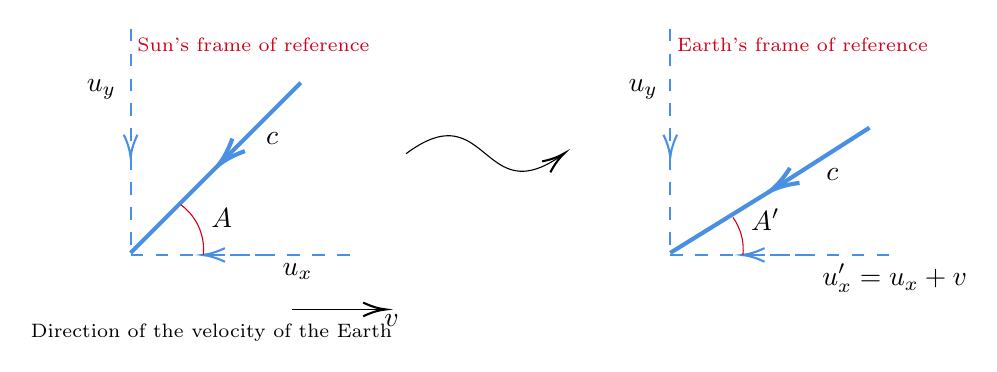
\begin{tikzpicture}[x=0.75pt,y=0.75pt,yscale=-1,xscale=1]
					%uncomment if require: \path (0,300); %set diagram left start at 0, and has height of 300
					
					%Straight Lines [id:da1945853252993458] 
					\draw [color={rgb, 255:red, 74; green, 144; blue, 226 }  ,draw opacity=1 ][line width=1.5]    (233.33,91.75) -- (195.45,129.63) ;
					\draw [shift={(193.33,131.75)}, rotate = 315] [color={rgb, 255:red, 74; green, 144; blue, 226 }  ,draw opacity=1 ][line width=1.5]    (14.21,-4.28) .. controls (9.04,-1.82) and (4.3,-0.39) .. (0,0) .. controls (4.3,0.39) and (9.04,1.82) .. (14.21,4.28)   ;
					%Straight Lines [id:da5062438778599464] 
					\draw [color={rgb, 255:red, 74; green, 144; blue, 226 }  ,draw opacity=1 ][line width=1.5]    (193.33,131.75) -- (151.33,173.75) ;
					%Straight Lines [id:da2563535626363741] 
					\draw [color={rgb, 255:red, 74; green, 144; blue, 226 }  ,draw opacity=1 ][line width=0.75]  [dash pattern={on 4.5pt off 4.5pt}]  (151.33,65.75) -- (151.33,125.75) ;
					\draw [shift={(151.33,127.75)}, rotate = 270] [color={rgb, 255:red, 74; green, 144; blue, 226 }  ,draw opacity=1 ][line width=0.75]    (10.93,-3.29) .. controls (6.95,-1.4) and (3.31,-0.3) .. (0,0) .. controls (3.31,0.3) and (6.95,1.4) .. (10.93,3.29)   ;
					%Straight Lines [id:da6709792968386992] 
					\draw [color={rgb, 255:red, 74; green, 144; blue, 226 }  ,draw opacity=1 ][line width=0.75]  [dash pattern={on 4.5pt off 4.5pt}]  (151.33,127.75) -- (151.33,173.75) ;
					%Straight Lines [id:da48943135811202587] 
					\draw [color={rgb, 255:red, 74; green, 144; blue, 226 }  ,draw opacity=1 ][line width=0.75]  [dash pattern={on 4.5pt off 4.5pt}]  (151.33,174.75) -- (221.33,174.75) ;
					%Straight Lines [id:da6386606946130312] 
					\draw [color={rgb, 255:red, 74; green, 144; blue, 226 }  ,draw opacity=1 ][line width=0.75]  [dash pattern={on 4.5pt off 4.5pt}]  (256.83,174.75) -- (187.83,174.75) ;
					\draw [shift={(185.83,174.75)}, rotate = 360] [color={rgb, 255:red, 74; green, 144; blue, 226 }  ,draw opacity=1 ][line width=0.75]    (10.93,-3.29) .. controls (6.95,-1.4) and (3.31,-0.3) .. (0,0) .. controls (3.31,0.3) and (6.95,1.4) .. (10.93,3.29)   ;
					%Straight Lines [id:da3769240929152531] 
					\draw    (229,201) -- (272.33,201) ;
					\draw [shift={(274.33,201)}, rotate = 180] [color={rgb, 255:red, 0; green, 0; blue, 0 }  ][line width=0.75]    (10.93,-3.29) .. controls (6.95,-1.4) and (3.31,-0.3) .. (0,0) .. controls (3.31,0.3) and (6.95,1.4) .. (10.93,3.29)   ;
					%Shape: Arc [id:dp7820806319031516] 
					\draw  [draw opacity=0] (175.48,150.52) .. controls (178.45,152.67) and (181.03,155.5) .. (182.99,158.93) .. controls (185.85,163.96) and (186.9,169.5) .. (186.33,174.75) -- (161.94,170.9) -- cycle ; \draw  [color={rgb, 255:red, 208; green, 2; blue, 27 }  ,draw opacity=1 ] (175.48,150.52) .. controls (178.45,152.67) and (181.03,155.5) .. (182.99,158.93) .. controls (185.85,163.96) and (186.9,169.5) .. (186.33,174.75) ;
					%Straight Lines [id:da2872174366196797] 
					\draw [color={rgb, 255:red, 74; green, 144; blue, 226 }  ,draw opacity=1 ][line width=1.5]    (507.33,113.42) -- (461.86,142.47) ;
					\draw [shift={(459.33,144.08)}, rotate = 327.43] [color={rgb, 255:red, 74; green, 144; blue, 226 }  ,draw opacity=1 ][line width=1.5]    (14.21,-4.28) .. controls (9.04,-1.82) and (4.3,-0.39) .. (0,0) .. controls (4.3,0.39) and (9.04,1.82) .. (14.21,4.28)   ;
					%Straight Lines [id:da9611733213506582] 
					\draw [color={rgb, 255:red, 74; green, 144; blue, 226 }  ,draw opacity=1 ][line width=1.5]    (459.33,144.08) -- (437.88,157.34) -- (411.33,173.75) ;
					%Straight Lines [id:da401789247777968] 
					\draw [color={rgb, 255:red, 74; green, 144; blue, 226 }  ,draw opacity=1 ][line width=0.75]  [dash pattern={on 4.5pt off 4.5pt}]  (411.33,65.75) -- (411.33,125.75) ;
					\draw [shift={(411.33,127.75)}, rotate = 270] [color={rgb, 255:red, 74; green, 144; blue, 226 }  ,draw opacity=1 ][line width=0.75]    (10.93,-3.29) .. controls (6.95,-1.4) and (3.31,-0.3) .. (0,0) .. controls (3.31,0.3) and (6.95,1.4) .. (10.93,3.29)   ;
					%Straight Lines [id:da4949167463507602] 
					\draw [color={rgb, 255:red, 74; green, 144; blue, 226 }  ,draw opacity=1 ][line width=0.75]  [dash pattern={on 4.5pt off 4.5pt}]  (411.33,127.75) -- (411.33,173.75) ;
					%Straight Lines [id:da594785516435984] 
					\draw [color={rgb, 255:red, 74; green, 144; blue, 226 }  ,draw opacity=1 ][line width=0.75]  [dash pattern={on 4.5pt off 4.5pt}]  (411.33,174.75) -- (481.33,174.75) ;
					%Straight Lines [id:da3215828895575572] 
					\draw [color={rgb, 255:red, 74; green, 144; blue, 226 }  ,draw opacity=1 ][line width=0.75]  [dash pattern={on 4.5pt off 4.5pt}]  (516.83,174.75) -- (447.83,174.75) ;
					\draw [shift={(445.83,174.75)}, rotate = 360] [color={rgb, 255:red, 74; green, 144; blue, 226 }  ,draw opacity=1 ][line width=0.75]    (10.93,-3.29) .. controls (6.95,-1.4) and (3.31,-0.3) .. (0,0) .. controls (3.31,0.3) and (6.95,1.4) .. (10.93,3.29)   ;
					%Shape: Arc [id:dp6084400727894748] 
					\draw  [draw opacity=0] (441.54,156.66) .. controls (442.05,157.38) and (442.54,158.14) .. (442.99,158.93) .. controls (445.85,163.96) and (446.9,169.5) .. (446.33,174.75) -- (421.94,170.9) -- cycle ; \draw  [color={rgb, 255:red, 208; green, 2; blue, 27 }  ,draw opacity=1 ] (441.54,156.66) .. controls (442.05,157.38) and (442.54,158.14) .. (442.99,158.93) .. controls (445.85,163.96) and (446.9,169.5) .. (446.33,174.75) ;
					%Curve Lines [id:da612631671806025] 
					\draw    (284,126) .. controls (308.33,107.75) and (316.51,122.71) .. (328.18,130.48) .. controls (335.47,135.33) and (344.13,137.38) .. (358.94,126.77) ;
					\draw [shift={(360.33,125.75)}, rotate = 503.13] [color={rgb, 255:red, 0; green, 0; blue, 0 }  ][line width=0.75]    (10.93,-3.29) .. controls (6.95,-1.4) and (3.31,-0.3) .. (0,0) .. controls (3.31,0.3) and (6.95,1.4) .. (10.93,3.29)   ;
					
					% Text Node
					\draw (215.33,114.75) node [anchor=north west][inner sep=0.75pt]   [align=left] {$\displaystyle c$};
					% Text Node
					\draw (223.33,177.75) node [anchor=north west][inner sep=0.75pt]   [align=left] {$\displaystyle u_{x}$};
					% Text Node
					\draw (129,89) node [anchor=north west][inner sep=0.75pt]   [align=left] {$\displaystyle u_{y}$};
					% Text Node
					\draw (102,207) node [anchor=north west][inner sep=0.75pt]  [font=\scriptsize] [align=left] {Direction of the velocity of the Earth};
					% Text Node
					\draw (272.33,202) node [anchor=north west][inner sep=0.75pt]   [align=left] {$\displaystyle v$};
					% Text Node
					\draw (189,151) node [anchor=north west][inner sep=0.75pt]   [align=left] {$\displaystyle A$};
					% Text Node
					\draw (153.33,68.75) node [anchor=north west][inner sep=0.75pt]  [font=\scriptsize,color={rgb, 255:red, 208; green, 2; blue, 27 }  ,opacity=1 ] [align=left] {Sun's frame of reference};
					% Text Node
					\draw (485.33,131.75) node [anchor=north west][inner sep=0.75pt]   [align=left] {$\displaystyle c$};
					% Text Node
					\draw (483.33,177.75) node [anchor=north west][inner sep=0.75pt]   [align=left] {$\displaystyle u_{x} '=u_{x} +v$};
					% Text Node
					\draw (390,89) node [anchor=north west][inner sep=0.75pt]   [align=left] {$\displaystyle u_{y}$};
					% Text Node
					\draw (449,151) node [anchor=north west][inner sep=0.75pt]   [align=left] {$\displaystyle A'$};
					% Text Node
					\draw (413.33,68.75) node [anchor=north west][inner sep=0.75pt]  [font=\scriptsize,color={rgb, 255:red, 208; green, 2; blue, 27 }  ,opacity=1 ] [align=left] {Earth's frame of reference};
					
					
					\end{tikzpicture}
					
				\end{center}
			
			From the classical method, we have the aberration angle $\theta=A'-A$ as:
				\begin{equation*}
				\begin{aligned}
					\tan\theta&=\frac{\tan \left(A^{\prime}\right)-\tan A}{1+\tan \left(A^{\prime}\right) \tan A}\\
					&=\frac{-(v / c) \sin A}{1+(v / c) \cos A}\\
					&=\frac{-(v / c) \sin A}{(\cos A)^{2}+(v / c) \cos A+(\sin A)^{2}}\approx -\frac{v}{c}\sin A
				\end{aligned}
				\end{equation*}
			
				\begin{center}
					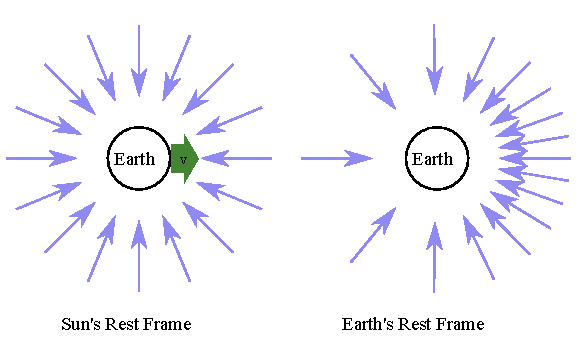
\includegraphics[scale=1]{sun-earth-aberration.pdf}
				\end{center}
		
			Using Lorentz transformation, we can see that:
				\begin{equation*}
				\begin{aligned}
					\begin{cases}
					u_x'=\frac{u_x+v}{1+u_xv/c^2}\\
					u_y'=\frac{u_y}{\gamma(1+u_xv/c^2)}
					\end{cases}
				\end{aligned}
				\end{equation*}
			
			The angle of the light in the Earth's frame is :
				\begin{equation*}
				\begin{aligned}
					\tan A'&=\frac{u_y'}{u_x'}=\frac{\sin A}{\gamma(v/c+\cos A)}\\
					\Rightarrow \tan \theta&=\tan (A'-A)=-\frac{\sin (A c (\gamma -1) \cos A+\gamma  v)}{c \gamma  \cos ^2A+c \sin ^2A+\gamma  v \cos A}\\
					&\approx -\frac{(\gamma -1) \sin 2 A}{(\gamma -1) \cos 2 A+\gamma +1}
				\end{aligned}
				\end{equation*}
		
		\subsubsection{}
			We set the light comes from the $xz$ plane, then the coordinate on the Riemann sphere can be described as $(r,\theta,\phi)=(cT,A,\phi)$, which correspond to the complex number (from the Stereographic projection in Exercise 4.50) 
				\begin{equation*}
				\begin{aligned}
					z=\frac{cT\sin A \cos \phi}{1+\cos A }+\mi\frac{cT\sin A \sin \phi}{1+\cos A } 
				\end{aligned}
				\end{equation*}
			
			The transformed point is $(cT,A',\phi)$, with the complex number:
				\begin{equation*}
				\begin{aligned}
					z'=\frac{cT\sin A' \cos \phi}{1+\cos A' }+\mi\frac{cT\sin A' \sin \phi}{1+\cos A' }
				\end{aligned}
				\end{equation*}
			
			Is a translation with respect to the $x$ axis. 
			\footnote{I may not understand this exercise properly, so I may write a wrong answer. If you know this better, please discuss with me. Thanks. }
		
	\subsection{Exercise 4.54}
		\subsubsection{}
			If I take the element: $a=4\frac{\sigma_x}{2}+6\mi \frac{\sigma_z}{2}$, we have:
				\begin{equation*}
				\begin{aligned}
					a=
					2\begin{pmatrix}
						0 & 1\\
						1 & 0
					\end{pmatrix}
					+3\mi 
					\begin{pmatrix}
					1 & 0\\
					0 & -1
					\end{pmatrix}
					=
					\begin{pmatrix}
					3\mi & 2\\
					2 & -3\mi 
					\end{pmatrix}
				\end{aligned}
				\end{equation*}
			
			With the exponential map, we have:
				\begin{equation*}
				\begin{aligned}
					\me ^a&=\sum_{n=0}^{\infty}\frac{1}{n!}
					\begin{pmatrix}
					3\mi & 2\\
					2 & -3\mi 
					\end{pmatrix}^n\\
					&=
					\left(
					\begin{array}{cc}
					\frac{1}{10} \me^{-\mi \sqrt{5}} \left(-3 \sqrt{5}+\me^{2 \mi \sqrt{5}} \left(3 \sqrt{5}+5\right)+5\right) & -\frac{\mi \me^{-\mi \sqrt{5}} \left(-1+\me^{2 \mi \sqrt{5}}\right)}{\sqrt{5}} \\
					-\frac{\mi \me^{-\mi \sqrt{5}} \left(-1+\me^{2 \mi \sqrt{5}}\right)}{\sqrt{5}} & \frac{1}{10} \me^{-\mi \sqrt{5}} \left(3 \sqrt{5}+\me^{2 \mi \sqrt{5}} \left(5-3 \sqrt{5}\right)+5\right) \\
					\end{array}
					\right)\\
					\Rightarrow &\det \me ^a=1
				\end{aligned}
				\end{equation*}
			
			Moreover, we can check it does form the Lie algebra. We first define:
				\begin{equation*}
				\begin{array}{cc}
					&K_1=\mi \frac{\sigma_x}{2},K_2=\mi \frac{\sigma_y}{2},K_3=\mi \frac{\sigma_z}{2}\\
					&J_1=\frac{\sigma_x}{2},J_2= \frac{\sigma_y}{2},J_3= \frac{\sigma_z}{2}
				\end{array}
				\end{equation*}
				
			If we compute its Lie bracket, we have:
				\begin{equation*}
				\begin{aligned}
					\left[K_i,K_j\right]&=-\mi \varepsilon_{ijk}J_k\\
					\left[J_i,J_j\right]&=\mi \varepsilon_{ijk}J_k\\
					\left[J_i,K_j\right]&=\mi \varepsilon_{ijk}K_k
				\end{aligned}
				\end{equation*}
			
		\subsubsection{}
			We have mentioned in Exercise 3.12, connected and compact group can be generated from the exponential map(otherwise we don't know). $SL(2,\mathbb{C})$ is not compact, and kant be generated from $\mathfrak{sl}(2,\mathbb{C})$. For example:
				\begin{equation*}
				\begin{aligned}
					\begin{pmatrix}
					-1 & 1\\
					1 & 0
					\end{pmatrix}
				\end{aligned}
				\end{equation*}
			
			can not be generated from $\mathfrak{sl}(2,\mathbb{C})$. 
		
		\subsubsection{}
			First, we prove that $\{\mathds{1}_2,\sigma_x,\sigma_y,\sigma_z\}$ form a well defined basis. To see this, we just need to show that they are linear independent. 
				\begin{equation*}
				\begin{aligned}
					&a\mathds{1}_2+b\sigma_x+c\sigma_y+d\sigma_z=0\\
					&\Rightarrow 
					\begin{pmatrix}
					a+d & b-c\mi\\
					b+c\mi & a-d
					\end{pmatrix}=0\\
					&\Rightarrow a=b=c=d=0
				\end{aligned}
				\end{equation*}
			
			So it is linear independent, which means it is a well defined. In this basis, the spacetime vector $\hat{x}=(x^0,x^1,x^2,x^3)$ can be written as:
				\begin{equation*}
				\begin{aligned}
					\begin{pmatrix}
						x^0+x^3 & x^1-x^2\mi\\
						x^1+x^2\mi & x^0-x^3
					\end{pmatrix}
				\end{aligned}
				\end{equation*}
			
			The norm can be calculated by the determinant:
				\begin{equation*}
				\begin{aligned}
					|\hat{x}|^2=-\det
					\begin{pmatrix}
					x^0+x^3 & x^1-x^2\mi\\
					x^1+x^2\mi & x^0-x^3
					\end{pmatrix}=-(x^0)^2+(x^1)^2+(x^2)^2+(x^3)^2
				\end{aligned}
				\end{equation*}
			
		\subsubsection{}
			If we think generally, we use a arbitrary matrix in $SL(2,\mathbb{C})$ to transform:
				\begin{equation*}
				\begin{aligned}
					\begin{pmatrix}
					x'^0+x'^3 & x'^1-x'^2\mi\\
					x'^1+x'^2\mi & x'^0-x'^3
					\end{pmatrix}
					=
					\begin{pmatrix}
					a+b\mi & c+d\mi\\
					e+f\mi & g+h\mi
					\end{pmatrix}
					\begin{pmatrix}
					x^0+x^3 & x^1-x^2\mi\\
					x^1+x^2\mi & x^0-x^3
					\end{pmatrix}
					\begin{pmatrix}
					a+b\mi & c+d\mi\\
					e+f\mi & g+h\mi
					\end{pmatrix}^{\dagger}
				\end{aligned}
				\end{equation*}
			
			If we compute the transformed coordinate, we have:
				\begin{equation*}
				\begin{aligned}
					\begin{cases}
						x'^0=&x^0 \frac{1}{2}\left(a^2+b^2+c^2+d^2+e^2+f^2+g^2+h^2\right)+x^3 \frac{1}{2}\left(a^2+b^2-c^2-d^2+e^2+f^2-g^2-h^2\right)\\&+x^1 ( a c+ b d+ e g+ f h)+x^2 (- a d+ b c- e h+ f g)\\
						x'^1=&x^0 (a e+b f+c g+d h)+x^1 (a g+b h+c e+d f)+x^2 (-a h+b g+c f-d e)+x^3 (a e+b f-c g-d h)\\
						x'^2=&x^0 (a f-b e+c h-d g)+x^1 (a h-b g+c f-d e)+x^2 (a g+b h-c e-d f)+x^3 (a f-b e-c h+d g)\\
						x'^3=&x^0 \frac{1}{2}\left(a^2+b^2+c^2+d^2-e^2-f^2-g^2-h^2\right)+x^3 \frac{1}{2}\left(a^2+b^2-c^2-d^2-e^2-f^2+g^2+h^2\right)\\&+x^1 ( a c+ b d- e g- f h)+x^2 (- a d+ b c+ e h- f g)
					\end{cases}
				\end{aligned}
				\end{equation*}
			
			With the condition $\det \mathcal{M}=1$:
				\begin{equation*}
				\begin{aligned}
					\begin{cases}
						a g-b h-c e+d f=1\\
						a h+b g-c f-d e=0
					\end{cases}
				\end{aligned}
				\end{equation*}
			
			So in general, the matrix in $SL(2,\mathbb{C})$ can transform a matrix $X$ encoded by $\hat{x}$. Now we consider the example. The matrix of boost in $z$ direction can be written by:
				\begin{equation*}
				\begin{aligned}
					\left(\begin{array}{cccc}
					\gamma & 0 & 0 & -\beta \gamma \\
					0 & 1 & 0 & 0 \\
					0 & 0 & 1 & 0 \\
					-\beta \gamma & 0 & 0 & \gamma
					\end{array}\right)
				\end{aligned}
				\end{equation*}
			
			With $v=0.5c$, we have $\beta=\frac{v}{c}=\frac{1}{2},\gamma=\frac{1}{\sqrt{1-\beta^2}}=\frac{2\sqrt{3}}{3}$. So the transformation matrix looks like:
				\begin{equation*}
				\begin{aligned}
					\left(\begin{array}{cccc}
					\frac{2\sqrt{3}}{3} & 0 & 0 & -\frac{\sqrt{3}}{3}\\
					0 & 1 & 0 & 0 \\
					0 & 0 & 1 & 0 \\
					-\frac{\sqrt{3}}{3} & 0 & 0 & \frac{2\sqrt{3}}{3}
					\end{array}\right)
				\end{aligned}
				\end{equation*}
			
			If we do the exponentiation of this generator $g_z$, we can see:
				\begin{equation*}
				\begin{aligned}
					\me^{a g_z}&=\sum_{n=0}^{\infty}\frac{1}{n!}
					\left(\begin{array}{cccc}
					0 & 0 & 0 & a\mi \\
					0 & 0 & 0 & 0 \\
					0 & 0 & 0 & 0 \\
					a\mi  & 0 & 0 & 0
					\end{array}\right)^n\\
					&=
					\left(\begin{array}{cccc}
					\cos a & 0 & 0 & \mi \sin a\\
					0 & 0 & 0 & 0 \\
					0 & 0 & 0 & 0 \\
					\mi \sin a  & 0 & 0 & \cos a
					\end{array}\right)
				\end{aligned}
				\end{equation*}
			
			Which means we should have:
				\begin{equation*}
				\begin{aligned}
					\begin{cases}
						\cos a=\frac{2\sqrt{3}}{3}\\
						\mi \sin a=-\frac{\sqrt{3}}{3}
					\end{cases}
					\Rightarrow a=\arccosh \mi \frac{2\sqrt{3}}{3}
				\end{aligned}
				\end{equation*}
			
			If it acts on a four vector, we can see:
				\begin{equation*}
				\begin{aligned}
					\hat{x'}=
					\left(\begin{array}{cccc}
					\frac{2\sqrt{3}}{3} & 0 & 0 & -\frac{\sqrt{3}}{3}\\
					0 & 1 & 0 & 0 \\
					0 & 0 & 1 & 0 \\
					-\frac{\sqrt{3}}{3} & 0 & 0 & \frac{2\sqrt{3}}{3}
					\end{array}\right)
					\begin{pmatrix}
					x^0\\
					x^1\\
					x^2\\
					x^3
					\end{pmatrix}
					=
					\begin{pmatrix}
					\frac{2\sqrt{3}}{3}x^0 -\frac{\sqrt{3}}{3}x^3\\
					x^1\\
					x^2\\
					-\frac{\sqrt{3}}{3}x^0+\frac{2\sqrt{3}}{3}x^3
					\end{pmatrix}
				\end{aligned}
				\end{equation*}
			
			The encoded matrix transforms as:
				\begin{equation*}
				\begin{aligned}
					X=
					\begin{pmatrix}
					x^0+x^3 & x^1-x^2\mi\\
					x^1+x^2\mi & x^0-x^3
					\end{pmatrix}
					\xlongrightarrow[]{MXM^{\dagger}}
					X'=
					\begin{pmatrix}
					\frac{\sqrt{3}}{3}(x^0+x^3) & x^1-x^2\mi\\
					x^1+x^2\mi & \sqrt{3}(x^0-x^3)
					\end{pmatrix}
				\end{aligned}
				\end{equation*}	
			
			We can set $\mathcal{M}$ as:
				\begin{equation*}
				\begin{aligned}
					\mathcal{M}_1=
					\begin{pmatrix}
					3^{-\frac{1}{4}} & 0\\
					0 & 3^{\frac{1}{4}}
					\end{pmatrix},
					\mathcal{M}_2=
					-\mathcal{M}_1=
					\begin{pmatrix}
					-3^{-\frac{1}{4}} & 0\\
					0 & -3^{\frac{1}{4}}
					\end{pmatrix}
				\end{aligned}
				\end{equation*}
			
			If we want to calculate $\mathcal{M}$ generally, we can derive the formular:
				\begin{equation*}
				\begin{aligned}
					\mathcal{M}(\Lambda)=\pm \frac{1}{\sqrt{\det\left(\Lambda^{\mu}_{\;\;\nu}\sigma_{\mu}\bar{\sigma}^{\nu}\right)}}\Lambda^{\mu}_{\;\;\nu}\sigma_{\mu}\bar{\sigma}^{\nu}
				\end{aligned}
				\end{equation*}
			
		\subsubsection{}
			I have figure out the general case for $\mathcal{M}$, so I don't think I need more example. 
		
		\subsubsection{}
			Of course $\mathcal{M}$ is not unique. Because for a transformation:
				\begin{equation*}
				\begin{aligned}
					X'=\mathcal{M}X\mathcal{M}^{\dagger}=(-\mathcal{M})X(-\mathcal{M}^{\dagger})
				\end{aligned}
				\end{equation*}
			
			Which means $\mathcal{M}$ and $-\mathcal{M}$ both satisfy the condition. So $\rho$ is in fact a lift of a projective representation, like the $\tilde{\rho}$ in Fig 4.16 in the note. So $\rho $ is just an "avatar" of the projective representation $SO^+(1,3)\rightarrow PSL(2,\mathbb{C})$. 
		
		\subsubsection{}
			We can choose the class of $\beta=1$, namely $[1]\in H^2 [\text{Mob},\mathbb{Z}_2]=\mathbb{Z}_2$. 
			\footnote{I'm not sure about this. Because I think if I choose $[-1]$ is also OK. }
	\subsection{Exercise 4.55*}
		\subsubsection*{1}
			Consider two $n$-cochains:
				\begin{equation*}
				\begin{aligned}
					&c_1(g_1,g_2,\cdots,g_n)=\me^{\mi \theta_1}\\
					&c_2(g_1,g_2,\cdots,g_n)=\me^{\mi \theta_2}
				\end{aligned}
				\end{equation*}
		
			Of course the identity is $c_0(g_1,g_2,\cdots,g_n)=1$, the inverse of $c_1$ is $c_1^{-1}(g_1,g_2,\cdots,g_n)=\me^{-\mi \theta_1}$. It is abelian because:
				\begin{equation*}
				\begin{aligned}
					c_1c_2=\me^{\mi( \theta_1+\theta_{2})}=c_2c_1
				\end{aligned}
				\end{equation*}
				
		\subsubsection*{2}
			This problem is pretty...tough. Just plug in, and you will find a way to prove it.
			\begin{equation*}
			\begin{aligned}
			&\di ^2c(g_0,\cdots,g_n,g_{n+1})\\
			=&\prod_{i=0}^{n+1}\di c(g_0,\cdots,g_{i-2},g_{i-1}g_{i},g_{i+1},\cdots,g_{n+1})^{(-1)^i}\\
			=&\frac{\overbrace{\di c(g_1,\cdots,g_{n+1})}^{\td{172}}\overbrace{\di c(g_0,g_1g_2,\cdots,g_{n+1})}^{\td{174}}\cdots \di c(g_0,g_1,\cdots,g_{i-1}g_i,\cdots,g_{n+1})\cdots \di c(g_0,g_1,\cdots,g_{n})}{\underbrace{\di c(g_0g_1,\cdots,g_{n+1})}_{\td{173}}\underbrace{\di c(g_0,g_1,g_2g_3,\cdots,g_{n+1})}_{\td{175}}\cdots\di c(g_0,g_1,\cdots,g_{i}g_{i+1},\cdots,g_{n+1})\cdots}
			\end{aligned}
			\end{equation*}
			
			Consider every term:
				\begin{equation*}
				\begin{aligned}
				\td{172}=\frac{\overbrace{c(g_2,\cdots g_{n+1})}^{1^{\text{st}}\text{ term of \td{173}}} \overbrace{c(g_1,g_2g_3,\cdots ,g_{n+1})}^{1^{\text{st}}\text{ term of \td{175}}}\cdots}{\underbrace{c(g_1g_2,\cdots,g_{n+1})}_{1^{\text{st}}\text{ term of \td{174}}}\cdots}
				\end{aligned}
				\end{equation*}
			
			We can see every term on the numerator of $\td{172}$ is the first term of those on the denominator of $\di ^2 c$. Then let's see $\td{173}$. 
				\begin{equation*}
				\begin{aligned}
				\td{173}=\frac{\overbrace{c(g_2,\cdots g_{n+1})}^{1^{\text{st}}\text{ term of \td{172}}} \overbrace{c(g_0g_1,g_2g_3,\cdots ,g_{n+1})}^{2^{\text{nd}}\text{ term of \td{175}}}\cdots}{\underbrace{c(g_0g_1g_2,\cdots,g_{n+1})}_{2^{\text{nd}}\text{ term of \td{174}}}\cdots}
				\end{aligned}
				\end{equation*}
			
			Notice that except for the first term(reduced with $\td{172}$), other term are the second term of others. Let's see $\td{174}$:
				\begin{equation*}
				\begin{aligned}
				\td{174}=\frac{\overbrace{c(g_1g_2,\cdots g_{n+1})}^{2^{\text{nd}}\text{ term of \td{172}}} \overbrace{c(g_0,g_1,g_2g_3g_4,\cdots ,g_{n+1})}^{3^{\text{rd}}\text{ term of \td{175}}}\cdots}{\underbrace{c(g_0g_1g_2,\cdots,g_{n+1})}_{2^{\text{nd}}\text{ term of \td{173}}}\cdots}
				\end{aligned}
				\end{equation*}
				
			We can see clearly that for the $n$-th term (call it \textcircled{$ n $}) in $\di ^2 c$, the $i$-th term($i<n$)(of \textcircled{$ n $}) is the $(n-1)$-th term of \textcircled{$i$}, the $j$-th term($j\geq n$) is the $n$-th term of 
			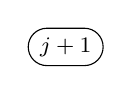
\begin{tikzpicture}[baseline=(char.base)]
			\node(char)[draw,fill=white,
			shape=rounded rectangle,
			minimum width=0.6cm]
			{\footnotesize $j+1$};
			\end{tikzpicture}
			. So every term can be reduced, which means $\di ^2 c=1$, it is nilpotent. 
		
		\subsubsection*{3}
			We first prove that exact cochains form a group. Suppose:
				\begin{equation*}
				\begin{aligned}
					c_1=\di c_1',c_2=\di c_2'
				\end{aligned}
				\end{equation*}
				
			We know that $n-1$-th cochains form a group, so we may set:
				\begin{equation*}
				\begin{aligned}
					c_1'c_2'=c_3'
				\end{aligned}
				\end{equation*}
				
			Consider:
				\begin{equation*}
				\begin{aligned}
					c_1c_2=&(\di c_1')(g_1,g_2,\cdots,g_n) (\di g_2')(g_1,g_2,\cdots,g_n)\\
					=&\prod_{i=0}^{n}c_1'(\cdots,g_{i-2},g_{i-1}g_{i},\cdots)\prod_{j=0}^{n}c_2'(\cdots,g_{j-2},g_{j-1}g_{j},\cdots)\\
					=&\prod_{i=0}^{n}c_1'(\cdots,g_{i-2},g_{i-1}g_{i},\cdots)c_2'(\cdots,g_{i-2},g_{i-1}g_{i},\cdots)\\
					=&\prod_{i=0}^{n}c_3'(\cdots,g_{i-2},g_{i-1}g_{i},\cdots)=\di c_3'
				\end{aligned}
				\end{equation*}
				
			Which means $c_1c_2$ is also exact. The identity is clearly exact because $\di ^2=1$. As for the inverse, I cannot prove the inverse is also exact yet. 
		
	
		
			
			
			
	
	\subsection{Exercise 4.56-4.60}
		Exercise with * will be constructed soon. 

\section{Interlude: Basic Algebraic Topology}
	\subsection{Exercise 5.1}
		Consider a set of three element: $X=\{a,b,c\}$. There are 29 topologies can be defined, and can be classified into nine kinds:
			\begin{enumerate}
				\item \{$\varnothing$, X\}
				\item \{$\varnothing$,\{$a$\},$X$\},\{$\varnothing$,\{$b$\},$X$\},\{$\varnothing$,\{$c$\},$X$\}
				\item \{$\varnothing$,\{$a$,$b$\},$X$\},\{$\varnothing$,\{$a$,$c$\},$X$\},\{$\varnothing$,\{$b$,$c$\},$X$\}
				\item \{$\varnothing$,\{$a$\},\{$b$,$c$\},$X$\},\{$\varnothing$,\{$b$\},\{$a$,$c$\},$X$\},\{$\varnothing$,\{$c$\},\{$a$,$b$\},$X$\}
				\item \{$\varnothing$,\{$a$\},\{$a$,$b$\},$X$\},\{$\varnothing$,\{$a$\},\{$a$,$c$\},$X$\},\{$\varnothing$,\{$b$\},\{$a$,$b$\},$X$\},\{$\varnothing$,\{$b$\},\{$b$,$c$\},$X$\},\{$\varnothing$,\{$c$\},\{$a$,$c$\},$X$\},\{$\varnothing$,\{$c$\},\{$b$,$c$\},$X$\}
				\item \{$\varnothing$,\{$a$\},\{$a$,$b$\},\{$a$,$c$\},$X$\},\{$\varnothing$,\{$b$\},\{$a$,$b$\},\{$b$,$c$\},$X$\},\{$\varnothing$,\{$c$\},\{$a$,$c$\},\{$b$,$c$\},$X$\}
				\item \{$\varnothing$,\{$a$\},\{$b$\},\{$a$,$b$\},$X$\},\{$\varnothing$,\{$a$\},\{$c$\},\{$a$,$c$\},$X$\},\{$\varnothing$,\{$b$\},\{$c$\},\{$b$,$c$\},$X$\}
				\item \{$\varnothing$,\{$a$\},\{$b$\},\{$a$,$b$\},\{$a$,$c$\},$X$\},\{$\varnothing$,\{$a$\},\{$b$\},\{$a$,$b$\},\{$b$,$c$\},$X$\},\{$\varnothing$,\{$a$\},\{$c$\},\{$a$,$b$\},\{$a$,$c$\},$X$\},\\\{$\varnothing$,\{$a$\},\{$c$\},\{$a$,$c$\},\{$b$,$c$\},$X$\},\{$\varnothing$,\{$b$\},\{$c$\},\{$a$,$b$\},\{$b$,$c$\},$X$\},\{$\varnothing$,\{$b$\},\{$c$\},\{$a$,$c$\},\{$b$,$c$\},$X$\}
				\item \{$\varnothing$,\{$a$\},\{$b$\},\{$c$\},\{$a$,$b$\},\{$a$,$c$\},\{$b$,$c$\},$X$\}
			\end{enumerate}
		
		In these topologies, the  mentioned set are all open set. Take \{$\varnothing$,\{$a$\},\{$b$\},\{$a$,$b$\},$X$\} for example: the set mentioned are open, sets $\varnothing$,\{$ c $\},\{$ a,c $\},\{$ b,c $\},$X$ are closed. $\varnothing$ and $X$ are both open and closed.
	\subsection{Exercise 5.2}
		\subsubsection{Axioms for Closed Sets}
			A topological space is a pair $(X, \mathcal{A})$ consisting of a set $X$ and a set $\mathcal{A}$ of subsets of $X$ (called "closed sets"), such that the following axioms hold:
				\begin{enumerate}
					\item Any (infinite) intersection of closed sets is closed.
					\item The union of any two closed sets (finite) is closed.
					\item $X$ and $\phi$ are closed.
				\end{enumerate}
					
			So if $M\subset X$ is closed, then $X\setminus M$ is open. 
		
		\subsubsection{Axioms for Neighborhood}
			A topological space is a pair $(X, \mathcal{U})$ consisting of a set $X$ and a family $\mathcal{U}=\left\{\mathcal{U}_{x}\right\}_{x \in X}$ of sets $\mathcal{U}_{x}$ of subsets of $X$ (called "neighborhoods of $x^{\prime \prime}$ ) such that:
				\begin{enumerate}
					\item Each neighborhood of $x$ contains $x$, and $X$ is a neighborhood of each of its points.
					\item If $V \subset X$ contains a neighborhood of $x$, then $V$ itself is a neighborhood of $x$
					\item The intersection of any two neighborhoods of $x$ is a neighborhood of $x$
					\item Each neighborhood of $x$ contains a neighborhood of $x$ that is also a neighborhood of each of its points.
				\end{enumerate}
	
			If a neighbourhood $U$ is the neighbourhood of every $x\in U$, then we call $U$ open. 
	
	\subsection{Exercise 5.3}
		We can define the distance of two rational number by:
			\begin{equation*}
			\begin{aligned}
				d(x,y)=|x-y|
			\end{aligned}
			\end{equation*}
		
		Which induce the metic topology. To say specifically, the family of sets are the "open discs" and their possible unions. 
			\begin{equation*}
			\begin{aligned}
				U_{\varepsilon}(X)=\{y\in X| d(x,y)=|x-y|<\varepsilon\}
			\end{aligned}
			\end{equation*}
	
	\subsection{Exercise 5.4}
		The topology of $E(N)$ is not connected. The reflection seperate $E^(N)$ into two connected part $E^+(N)$ and $E^-(N)$. 
			\begin{center}
				
				
				\tikzset{every picture/.style={line width=0.75pt}} %set default line width to 0.75pt        
				
				\begin{tikzpicture}[x=0.75pt,y=0.75pt,yscale=-1,xscale=1]
				%uncomment if require: \path (0,300); %set diagram left start at 0, and has height of 300
				
				%Shape: Arc [id:dp30874875169618143] 
				\draw  [draw opacity=0] (216.65,72.26) .. controls (223.56,72.02) and (230.39,73.42) .. (236.69,76.63) .. controls (260.53,88.8) and (267.7,122.47) .. (252.7,151.84) .. controls (244.48,167.95) and (231.3,179.42) .. (217.15,184.49) -- (209.54,129.81) -- cycle ; \draw   (216.65,72.26) .. controls (223.56,72.02) and (230.39,73.42) .. (236.69,76.63) .. controls (260.53,88.8) and (267.7,122.47) .. (252.7,151.84) .. controls (244.48,167.95) and (231.3,179.42) .. (217.15,184.49) ;
				%Shape: Arc [id:dp2471691798425928] 
				\draw  [draw opacity=0] (371.09,182.93) .. controls (361.9,180.11) and (353.29,174.99) .. (346.17,167.59) .. controls (323.55,144.09) and (324.47,106.5) .. (348.23,83.63) .. controls (355.72,76.41) and (364.6,71.52) .. (373.94,68.95) -- (389.19,126.18) -- cycle ; \draw   (371.09,182.93) .. controls (361.9,180.11) and (353.29,174.99) .. (346.17,167.59) .. controls (323.55,144.09) and (324.47,106.5) .. (348.23,83.63) .. controls (355.72,76.41) and (364.6,71.52) .. (373.94,68.95) ;
				%Straight Lines [id:da6814453885696405] 
				\draw    (200,237.42) ;
				%Straight Lines [id:da6752357095439954] 
				\draw    (259,130.42) ;
				\draw [shift={(259,130.42)}, rotate = 0] [color={rgb, 255:red, 0; green, 0; blue, 0 }  ][fill={rgb, 255:red, 0; green, 0; blue, 0 }  ][line width=0.75]      (0, 0) circle [x radius= 3.35, y radius= 3.35]   ;
				%Straight Lines [id:da9765104550133347] 
				\draw    (330.5,130.58) ;
				\draw [shift={(330.5,130.58)}, rotate = 0] [color={rgb, 255:red, 0; green, 0; blue, 0 }  ][fill={rgb, 255:red, 0; green, 0; blue, 0 }  ][line width=0.75]      (0, 0) circle [x radius= 3.35, y radius= 3.35]   ;
				%Curve Lines [id:da2935362377843693] 
				\draw    (277,132.17) .. controls (299.54,113.55) and (288.47,139.11) .. (312.49,129.78) ;
				\draw [shift={(314,129.17)}, rotate = 517.0699999999999] [color={rgb, 255:red, 0; green, 0; blue, 0 }  ][line width=0.75]    (10.93,-3.29) .. controls (6.95,-1.4) and (3.31,-0.3) .. (0,0) .. controls (3.31,0.3) and (6.95,1.4) .. (10.93,3.29)   ;
				
				% Text Node
				\draw (184,120.82) node [anchor=north west][inner sep=0.75pt]    {$E^{-}( N)$};
				% Text Node
				\draw (351,120.82) node [anchor=north west][inner sep=0.75pt]    {$E^{+}( N)$};
				% Text Node
				\draw (261,133.82) node [anchor=north west][inner sep=0.75pt]    {$I^{-}$};
				% Text Node
				\draw (316,132.57) node [anchor=north west][inner sep=0.75pt]    {$I$};
				
				
				\end{tikzpicture}
				
			\end{center}
		
		Also, $O(1,3)$ is not connected. It can be decomposed into four connected part as said in Exercise 4.52. You should also notice that  $SO(1,3)$ is also not connected and can be splited into 2 parts, which is not like $SO(N)$, which is connected. 
			
			\subsubsection{More information}
				The topology of the indefinite orthogonal group $O(p,q)$ is pretty interesting. We have notice that $O(p,q)$ has four parts. $SO^+(p,q)$ is called the \textbf{identity component} of $O(1,3)$. The identity component of a topological group $ G $ is the connected component $ G^0 $ of $ G $ that contains the identity element of the group. The \textbf{identity path component }of a topological group $ G $ is the path(connected) component of $ G $ that contains the identity element of the group. The quotient group $ G/G^0 $ is called the group of components or component group of $ G $. Its elements are just the connected components of $ G $. One may similarly define the path component group as the group of path components. The path component group is just the \textbf{zeroth} homotopy group. So the \textbf{0}-th homotopy group of $O(p,q)$ is our old friend: the Klein four-group
					\begin{equation*}
					\begin{aligned}
						\pi _0(O(p,q))\cong Z_2\times Z_2
					\end{aligned}
					\end{equation*}
				
				And for $SO(p,q)$ is of course $Z_2$. 
				
				The group $ O(p, q) $ is also not compact, but contains the compact subgroups $ O(p) $ and $ O(q) $ acting on the subspaces on which the form is definite. In fact, $ O(p) \times O(q) $ is a \textbf{maximal compact subgroup} of $ O(p, q) $, while $ S(O(p) \times  O(q)) $ is a maximal compact subgroup of $ SO(p, q) $. Likewise, $ SO(p) \times SO(q) $ is a maximal compact subgroup of $ SO^+(p, q) $. 
				
				In particular, the fundamental group of $ SO^+(p, q) $ is the product of the fundamental groups of the components:
					\begin{equation*}
					\begin{aligned}
						\pi_1(SO^+(p, q))=\pi_1(SO(p)) \times  \pi_1(SO(q))
					\end{aligned}
					\end{equation*}
					
				The fundamental group of $ SO^+(p, q) $ is:
					\begin{center}
							\begin{tabular}{|l|l|l|l|}
								\hline
								$\pi_1(SO^+(p,q))$ & $p=1$ & $p=2$         & $p\geq 3$       \\ \hline
								$q=1$              & $Z_1$ & $Z$           & $Z_2$           \\ \hline
								$q=2$              & $Z$   & $Z\times Z$   & $Z\times Z_2$   \\ \hline
								$q\geq 3$          & $Z_2$ & $Z\times Z_2$ & $Z_2\times Z_2$ \\ \hline
							\end{tabular}
					\end{center}
	
	\subsection{Exercise 5.5}
		Remember the definition of Hausdorff space: If for an arbitrary pair of distinct points $x,x'\in X$, there always exist neighbourhoods $U_x$ of $x$ and $U_{x'}$ of $x'$ such that $U_x\cap U_{x'}=\emptyset$. 
		
		Let's consider $X=\mathbb{R}$ with usual topology. For two arbitrary points $a,b$ (assume $ a<b $) consider their neighbourhood: 	
			\begin{equation*}
			\begin{aligned}
				&U_a=(\frac{3a-b}{2},\frac{a+b}{2})\\
				&U_b=(\frac{a+b}{2},\frac{3b-a}{2})\\
				&\Rightarrow U_a\cap U_b=\emptyset
			\end{aligned}
			\end{equation*}
			
		So $X=\mathbb{R}$ with usual topology is a Hausdorff space. If $X=\mathbb{R}^n$ with usual topology, just divide the line $ab$ into two part to get two disjoint neighbourhood. Set $d(a,b)=r$, then the open ball $B_{\frac{r}{2}}(a),B_{\frac{r}{2}}(b)$ are two disjoint neighbourhood. 
	
	\subsection{Exercise 5.6}
		First we assume that for any open set $ U\in \mathbb{R}^n, f^{-1}(U) $  is an open set in $ R^m $. Which means for a open ball of $f(a)$ of radius $\varepsilon$:
			\begin{equation*}
			\begin{aligned}
				B_{\varepsilon}(f(a))=\{y|d^n(f(a)-y)<\varepsilon\}
			\end{aligned}
			\end{equation*}
			
		It is open in $\mathbb{R}^n$, hence $f^{-1}(B_{\varepsilon}(f(a)))$ is open in $ R^m $. Since $a\in f^{-1}(B_{\varepsilon}(f(a)))$, there exists some ball of radius $\delta>0$ about $a$ such that
			\begin{equation*}
			\begin{aligned}
				B_{\delta}(a)\subseteq f^{-1}(B_{\varepsilon}(f(a)))
			\end{aligned}
			\end{equation*}
			
		And this is the $\varepsilon-\delta$ criterion: if $a\in R^m$ such that $d(x,a)<\delta$, then $d(f(x),f(a))<\varepsilon$.
		
		Inversely, if the $\varepsilon-\delta$ criterion holds and let $U\subseteq \mathbb{R}^n$ be open. By definition, for each $y\in U$, there exist some $\varepsilon_y>0$, s.t:
			\begin{equation*}
			\begin{aligned}
				B_{\varepsilon_y}(y)\subseteq  U
			\end{aligned}
			\end{equation*}
		
		And we have:
			\begin{equation*}
			\begin{aligned}
				U=\bigcup_{y\in U}B_{\varepsilon_y}(y)
			\end{aligned}
			\end{equation*}
		
		Next we prove that $f^{-1}(U)$ is open in $ \mathbb{R}^m $. Suppose $x_0\in f^{-1}(U)$, then $f(x_0)\in U$, which means $f(x_0)\in B_{\varepsilon_{y_0}}(y_0)$ for some $y_0\in U$(We can see that $f(x_0)=y_0$). By definition, for some $\varepsilon_{y_0}>0$, if 
			\begin{equation*}
			\begin{aligned}
				d(f(x),f(x_0))<\varepsilon_{y_0}
			\end{aligned}
			\end{equation*}
		
		there exist some $\delta$, such that for $x\in \mathbb{R}$, 
			\begin{equation*}
			\begin{aligned}
				d(x,x_0)<\delta\Rightarrow B_{\delta}(x_0)\subseteq f^{-1}(U)
			\end{aligned}
			\end{equation*}
			
		since $x_0$ is an arbitrary in $f^{-1}(U)$ and has a open ball around it still in $f^{-1}(U)$, so $f^{-1}(U)$ is open, which finishes the proof. 
			
	\subsection{Exercise 5.7}
		We first prove that $(x,v)\sim (y,w)$ is indeed an equivalence relation. 
			\begin{enumerate}
				\item Reflective: If $ (x,v)\sim (x,v) $, which means we need some $g^{\alpha}_{\beta}$, such that$ v=g^{\alpha}_{\beta}v $, but we know that $v=v$, so just set $g^{\alpha}_{\beta}=\operatorname{id}=g^{\alpha}_{\alpha}$ is ok.
				\item Symmetric: If $(x,v)\sim (x,w)$, then we need to prove $(x,w)\sim (x,v)$. We know that $ v=g^{\alpha}_{\beta}w $, which means $ w=(g^{\alpha}_{\beta})^{-1}v $ and we want to find some $g^{\gamma}_{\delta}$, such that $ w=g^{\gamma}_{\delta}v $. From the relation:
					\begin{equation*}
					\begin{aligned}
						g^{\gamma}_{\alpha}g^{\beta}_{\gamma}g^{\alpha}_{\beta}=\operatorname{id}
					\end{aligned}
					\end{equation*}
					
					Set $\gamma =\alpha$ and we will get:
					\begin{equation*}
					\begin{aligned}
					g^{\alpha}_{\alpha}g^{\beta}_{\alpha}g^{\alpha}_{\beta}=\operatorname{id}g^{\beta}_{\alpha}g^{\alpha}_{\beta}=\operatorname{id}\Rightarrow g^{\beta}_{\alpha}=(g^{\alpha}_{\beta})^{-1}
					\end{aligned}
					\end{equation*}
					
					So $ w= g^{\beta}_{\alpha}v $ which means $(x,w)\sim (x,v)$. 
					\item Transitive: If $(x,v_{\alpha})\sim (x,v_{\beta}),(x,v_{\beta})\sim (x,v_{\gamma})$, then :
						\begin{equation*}
						\begin{aligned}
							v_{\alpha}=g^{\beta}_{\alpha}v_{\beta}=g^{\beta}_{\alpha}g^{\gamma}_{\beta}v_{\gamma}
						\end{aligned}
						\end{equation*}
					
					but we have:
						\begin{equation*}
						\begin{aligned}
							g_{\alpha}^{\gamma} g_{\gamma}^{\beta} g_{\beta}^{\alpha}=\operatorname{id}\Rightarrow g_{\alpha}^{\gamma}=g^{\beta}_{\alpha}g^{\gamma}_{\beta}
						\end{aligned}
						\end{equation*}
						
					So:
						\begin{equation*}
						\begin{aligned}
						v_{\alpha}=g_{\alpha}^{\gamma}v_{\gamma}\Rightarrow (x,v_{\alpha})\sim (x,v_{\gamma})
						\end{aligned}
						\end{equation*}
			\end{enumerate}
		
			\subsubsection{}
				Using the picture, I think there's nothing I need to prove. 
					\begin{center}
						
						
						\tikzset{every picture/.style={line width=0.75pt}} %set default line width to 0.75pt        
						
						\begin{tikzpicture}[x=0.75pt,y=0.75pt,yscale=-1,xscale=1]
						%uncomment if require: \path (0,300); %set diagram left start at 0, and has height of 300
						
						%Straight Lines [id:da3095848292054164] 
						\draw [color={rgb, 255:red, 144; green, 19; blue, 254 }  ,draw opacity=1 ]   (108.83,99) -- (398.5,99) ;
						%Straight Lines [id:da1473110432477247] 
						\draw [color={rgb, 255:red, 144; green, 19; blue, 254 }  ,draw opacity=1 ]   (288,17.52) -- (288,99) ;
						%Straight Lines [id:da3763448354077161] 
						\draw [color={rgb, 255:red, 144; green, 19; blue, 254 }  ,draw opacity=1 ]   (308,17.52) -- (308,99) ;
						%Straight Lines [id:da1093455862487911] 
						\draw [color={rgb, 255:red, 144; green, 19; blue, 254 }  ,draw opacity=1 ]   (326,17.52) -- (326,99) ;
						%Straight Lines [id:da8760281833352676] 
						\draw [color={rgb, 255:red, 144; green, 19; blue, 254 }  ,draw opacity=1 ]   (345,17.52) -- (345,99) ;
						%Straight Lines [id:da8729174123916915] 
						\draw [color={rgb, 255:red, 144; green, 19; blue, 254 }  ,draw opacity=1 ]   (362,17.52) -- (362,99) ;
						%Straight Lines [id:da7515069477402684] 
						\draw [color={rgb, 255:red, 245; green, 166; blue, 35 }  ,draw opacity=1 ]   (289,153) -- (622.5,153) ;
						%Straight Lines [id:da8304046464257157] 
						\draw [color={rgb, 255:red, 245; green, 166; blue, 35 }  ,draw opacity=1 ]   (300,104) -- (300,153) ;
						%Straight Lines [id:da2749741536862421] 
						\draw [color={rgb, 255:red, 245; green, 166; blue, 35 }  ,draw opacity=1 ]   (320,104) -- (320,153) ;
						%Straight Lines [id:da379987125453901] 
						\draw [color={rgb, 255:red, 245; green, 166; blue, 35 }  ,draw opacity=1 ]   (338,104) -- (338,153) ;
						%Straight Lines [id:da9719293782275581] 
						\draw [color={rgb, 255:red, 245; green, 166; blue, 35 }  ,draw opacity=1 ]   (357,104) -- (357,153) ;
						%Straight Lines [id:da6074912963459046] 
						\draw [color={rgb, 255:red, 245; green, 166; blue, 35 }  ,draw opacity=1 ]   (374,104) -- (374,153) ;
						%Straight Lines [id:da8163676613277628] 
						\draw [color={rgb, 255:red, 208; green, 2; blue, 27 }  ,draw opacity=1 ]   (126,194) -- (459.5,194) ;
						%Straight Lines [id:da6416749738467443] 
						\draw [color={rgb, 255:red, 208; green, 2; blue, 27 }  ,draw opacity=1 ]   (367,155) -- (367,194) ;
						%Straight Lines [id:da005428385953028081] 
						\draw [color={rgb, 255:red, 208; green, 2; blue, 27 }  ,draw opacity=1 ]   (387,155) -- (387,194) ;
						%Straight Lines [id:da5499992591565003] 
						\draw [color={rgb, 255:red, 208; green, 2; blue, 27 }  ,draw opacity=1 ]   (405,155) -- (405,194) ;
						%Straight Lines [id:da710716768267143] 
						\draw [color={rgb, 255:red, 208; green, 2; blue, 27 }  ,draw opacity=1 ]   (424,155) -- (424,194) ;
						%Straight Lines [id:da3428482930200688] 
						\draw [color={rgb, 255:red, 208; green, 2; blue, 27 }  ,draw opacity=1 ]   (441,155) -- (441,194) ;
						%Straight Lines [id:da22768842903689357] 
						\draw [color={rgb, 255:red, 74; green, 144; blue, 226 }  ,draw opacity=1 ]   (6,272) -- (646.37,272) ;
						%Straight Lines [id:da025101093595356394] 
						\draw [color={rgb, 255:red, 74; green, 144; blue, 226 }  ,draw opacity=1 ]   (6,236) -- (646.37,236) ;
						%Straight Lines [id:da6817714342383824] 
						\draw [color={rgb, 255:red, 208; green, 2; blue, 27 }  ,draw opacity=1 ]   (354,197) -- (354,236) ;
						%Straight Lines [id:da018098670719812415] 
						\draw [color={rgb, 255:red, 208; green, 2; blue, 27 }  ,draw opacity=1 ]   (372,197) -- (372,236) ;
						%Straight Lines [id:da024675608431722118] 
						\draw [color={rgb, 255:red, 208; green, 2; blue, 27 }  ,draw opacity=1 ]   (392,197) -- (392,236) ;
						%Straight Lines [id:da3399669287296432] 
						\draw [color={rgb, 255:red, 208; green, 2; blue, 27 }  ,draw opacity=1 ]   (411,197) -- (411,236) ;
						%Straight Lines [id:da32354731352869415] 
						\draw [color={rgb, 255:red, 208; green, 2; blue, 27 }  ,draw opacity=1 ]   (428,197) -- (428,236) ;
						%Straight Lines [id:da9459394210885452] 
						\draw [color={rgb, 255:red, 144; green, 19; blue, 254 }  ,draw opacity=1 ]   (302,202.18) -- (302,236) ;
						%Straight Lines [id:da9600683076127041] 
						\draw [color={rgb, 255:red, 144; green, 19; blue, 254 }  ,draw opacity=1 ]   (322,202.18) -- (322,236) ;
						%Straight Lines [id:da004545483344375212] 
						\draw [color={rgb, 255:red, 144; green, 19; blue, 254 }  ,draw opacity=1 ]   (340,202.18) -- (340,236) ;
						%Straight Lines [id:da3634523004839483] 
						\draw [color={rgb, 255:red, 144; green, 19; blue, 254 }  ,draw opacity=1 ]   (359,202.18) -- (359,236) ;
						%Straight Lines [id:da5758135007674333] 
						\draw [color={rgb, 255:red, 144; green, 19; blue, 254 }  ,draw opacity=1 ]   (378,202.18) -- (378,236) ;
						%Straight Lines [id:da7187394840678256] 
						\draw [color={rgb, 255:red, 144; green, 19; blue, 254 }  ,draw opacity=1 ]   (264,202.18) -- (264,236) ;
						%Straight Lines [id:da6399353302173956] 
						\draw [color={rgb, 255:red, 144; green, 19; blue, 254 }  ,draw opacity=1 ]   (284,202.18) -- (284,236) ;
						%Straight Lines [id:da4730210111416101] 
						\draw [color={rgb, 255:red, 144; green, 19; blue, 254 }  ,draw opacity=1 ]   (204,202.18) -- (204,236) ;
						%Straight Lines [id:da7277595977637925] 
						\draw [color={rgb, 255:red, 144; green, 19; blue, 254 }  ,draw opacity=1 ]   (224,202.18) -- (224,236) ;
						%Straight Lines [id:da3368795212216995] 
						\draw [color={rgb, 255:red, 144; green, 19; blue, 254 }  ,draw opacity=1 ]   (242,202.18) -- (242,236) ;
						%Straight Lines [id:da6232403885797648] 
						\draw [color={rgb, 255:red, 144; green, 19; blue, 254 }  ,draw opacity=1 ]   (166,202.18) -- (166,236) ;
						%Straight Lines [id:da034910593923154876] 
						\draw [color={rgb, 255:red, 144; green, 19; blue, 254 }  ,draw opacity=1 ]   (186,202.18) -- (186,236) ;
						%Straight Lines [id:da9365935415332799] 
						\draw [color={rgb, 255:red, 245; green, 166; blue, 35 }  ,draw opacity=1 ]   (444,201.18) -- (444,236) ;
						%Straight Lines [id:da20913355720526305] 
						\draw [color={rgb, 255:red, 245; green, 166; blue, 35 }  ,draw opacity=1 ]   (464,201.18) -- (464,236) ;
						%Straight Lines [id:da2929379751583431] 
						\draw [color={rgb, 255:red, 245; green, 166; blue, 35 }  ,draw opacity=1 ]   (482,201.18) -- (482,236) ;
						%Straight Lines [id:da26919054637535167] 
						\draw [color={rgb, 255:red, 245; green, 166; blue, 35 }  ,draw opacity=1 ]   (501,201.18) -- (501,236) ;
						%Straight Lines [id:da5810741558206765] 
						\draw [color={rgb, 255:red, 245; green, 166; blue, 35 }  ,draw opacity=1 ]   (518,201.18) -- (518,236) ;
						%Straight Lines [id:da4042448182065528] 
						\draw [color={rgb, 255:red, 245; green, 166; blue, 35 }  ,draw opacity=1 ]   (538,201.18) -- (538,236) ;
						%Straight Lines [id:da7995552645408248] 
						\draw [color={rgb, 255:red, 245; green, 166; blue, 35 }  ,draw opacity=1 ]   (558,201.18) -- (558,236) ;
						%Straight Lines [id:da70697937282467] 
						\draw [color={rgb, 255:red, 245; green, 166; blue, 35 }  ,draw opacity=1 ]   (576,201.18) -- (576,236) ;
						%Straight Lines [id:da5977996511564254] 
						\draw [color={rgb, 255:red, 245; green, 166; blue, 35 }  ,draw opacity=1 ]   (595,201.18) -- (595,236) ;
						%Straight Lines [id:da18801893709816275] 
						\draw [color={rgb, 255:red, 245; green, 166; blue, 35 }  ,draw opacity=1 ]   (612,201.18) -- (612,236) ;
						%Straight Lines [id:da7085546082739327] 
						\draw [color={rgb, 255:red, 245; green, 166; blue, 35 }  ,draw opacity=1 ]   (402,201.18) -- (402,236) ;
						%Straight Lines [id:da3669998395674733] 
						\draw [color={rgb, 255:red, 245; green, 166; blue, 35 }  ,draw opacity=1 ]   (419,201.18) -- (419,236) ;
						%Shape: Brace [id:dp36408101634524503] 
						\draw   (105,31.52) .. controls (100.33,31.52) and (98,33.85) .. (98,38.52) -- (98,101.02) .. controls (98,107.69) and (95.67,111.02) .. (91,111.02) .. controls (95.67,111.02) and (98,114.35) .. (98,121.02)(98,118.02) -- (98,183.52) .. controls (98,188.19) and (100.33,190.52) .. (105,190.52) ;
						
						% Text Node
						\draw (250,48.4) node [anchor=north west][inner sep=0.75pt]    {$\cdots $};
						% Text Node
						\draw (400,121.4) node [anchor=north west][inner sep=0.75pt]    {$\cdots $};
						% Text Node
						\draw (327,169.63) node [anchor=north west][inner sep=0.75pt]    {$\cdots $};
						% Text Node
						\draw (614,246) node [anchor=north west][inner sep=0.75pt]   [align=left] {$\displaystyle M$};
						% Text Node
						\draw (168,63.4) node [anchor=north west][inner sep=0.75pt]    {$U_{\alpha }$};
						% Text Node
						\draw (452,128.4) node [anchor=north west][inner sep=0.75pt]    {$U_{\beta }$};
						% Text Node
						\draw (231,171.4) node [anchor=north west][inner sep=0.75pt]    {$U_{\gamma }$};
						% Text Node
						\draw (16,209.4) node [anchor=north west][inner sep=0.75pt]  [font=\footnotesize]  {$E=\left( \bigsqcup _{\alpha }\left( U_{\alpha } \times \mathbb{R}^{k}\right)\right) /\sim \ $};
						% Text Node
						\draw (337.1,98.5) node [anchor=north west][inner sep=0.75pt]  [rotate=-90]  {$\sim $};
						% Text Node
						\draw (7,103.4) node [anchor=north west][inner sep=0.75pt]  [font=\footnotesize]  {$\bigsqcup _{\alpha }\left( U_{\alpha } \times \mathbb{R}^{k}\right) \ $};
						% Text Node
						\draw (388.1,152.5) node [anchor=north west][inner sep=0.75pt]  [rotate=-90]  {$\sim $};
						
						
						\end{tikzpicture}
						
					\end{center}
		
		\subsubsection{}
			Because we know $M$ is a Hausdorff space, so for $\forall x,y\in M$, there exist neighbourhood $N(x),N(y)$, s.t:
				\begin{equation*}
				\begin{aligned}
					N(x)\cap N(y)=\emptyset
				\end{aligned}
				\end{equation*}
			
			So for any pair $(x,v_1),(y,v_2)$, let:
				\begin{equation*}
				\begin{aligned}
					&N((x,v_1))=(N(x),v_1)\\
					&N((y,v_2))=(N(y),v_2)\\
					\Rightarrow &N((x,v_1))\cap N((y,v_2))=\emptyset
				\end{aligned}
				\end{equation*}
			
			Which means $E$ is also Hausdorff.
			
			About the fiber bundle of $PSL(2,\mathbb{C})$, I think the Mobius transformation may be the transition funciton.  
		
	\subsection{Exercise 5.8}
		The interval $(0,1)$ is not compact. Consider its open cover:
			\begin{equation*}
			\begin{aligned}
				\bigcup_{n=1}^{\infty} (\frac{1}{n},1)
			\end{aligned}
			\end{equation*}
		
		Do not have any finite open cover. So it is not compact. Similarly, for a  interval $(0,\infty]$, it is neither open or closed, because its complement $(\infty,0) $ is not open. We can construct a open cover:
			\begin{equation*}
			\begin{aligned}
				\bigcup_{n=1}^{\infty} (-1,n)
			\end{aligned}
			\end{equation*} 
		
		It also do not have any finite sub cover. We can see that compact needs closeness and boundary. 
	
	\subsection{Exercise 5.9}
		Consider a infinite open cover $P=\{U\}$ of $[a,b]$, and it do not have any finite subcover. So \textbf{at least one }of $[a,\frac{a+b}{2}]$ and $[\frac{a+b}{2},b]$ cannot be covered finitely. Call this interval $I_1$, we can then divide this interval into two parts, call the interval that cannot be covered finitely $I_2$.
		
		In this way a nested sequence $I_{1} \supset I_{2} \supset \cdots \supset I_{n} \supset \cdots$ of closed interval arises, none of which admit a covering by a finite subsystem of $P$. Since the length of the interval $I_{n}$ is $\left|I_{n}\right|=\left|I_{1}\right| \cdot 2^{-n},$ the sequence $\left\{I_{n}\right\}$ contain intervals of arbitrarily small length. But the nested interval theorem(Chinese: 闭区间套定理) implies that there exists a point $c$ belonging to all of the intervals $I_{n}, n \in \mathbb{N} .$ since $c \in I_{1}=[a, b]$ there exist an open interval $(\alpha, \beta)=U \in P \text { containing } c, \text { that is, } \alpha<c<\beta \text { . Let } \varepsilon=$ $\min \{c-\alpha, \beta-c\} .$ In the sequence just constructed, we find an interval $I_{n}$ such that $\left|I_{n}\right|<\varepsilon$. since $c \in I_{n}$ and $\left|I_{n}\right|<\varepsilon,$ we conclude that $I_{n} \subset U= (\alpha-\beta)$, But this contradicts the fact that the interval $I_{n}$ cannot be covered by a finite set of intervals from the system.
	
	\subsection{Exercise 5.10}
		To prove this theorem, we just need to prove: If a set $U\in \mathbb{R}^n$ is not compact, there exists an infinite sequence $x_n$ has no subsequence converging to a point in $U$. Because it is non-compact, there exists an infinite cover $\{U_{\alpha}\}$ with no finite subcover. Then we can construct:
			\begin{equation*}
			\begin{aligned}
				&x_0\in U_0\\
				&x_1\in U_1, x_1\not\in U_0\\
				&x_2\in U_2, x_2\not \in U_1,U_0\\
				&x_n\in U_n, x_2\not \in \bigcup_{i=0}^{n-1}U_i
			\end{aligned}
			\end{equation*}
		
		We can see such a infinite sequence converges to a boundary point or infinity. Also, for any subsequence $x_{n_k}$, if you claim 
			\begin{equation*}
			\begin{aligned}
				\lim_{k\rightarrow\infty}x_{n_k}=p\in U
			\end{aligned}
			\end{equation*}
		
		Then there exist $U_i,p\in U_i$ but according to the definition, $x_{n_{k+1}}\not \in U_i$, so we can construct two neighbourhood, s.t.:
			\begin{equation*}
			\begin{aligned}
				N(x_{n_k})\cap x_{n_{k+1}}=\emptyset
			\end{aligned}
			\end{equation*}
		
		It contradict to the definition of the limitation. So it must be compact. 
	
	\subsection{Exercise 5.11}
		According to theorem 5.1, we can see that if $\lim_{n\rightarrow \infty}x_n=a$, then $\lim_{n\rightarrow \infty}f(x_n)=f(a)$, which means the image $f(x)$ is compact in $\mathbb{R}$. So according to the Heine-Borel theorem, the image set is bounded and closed. So according to intermediate value theorem, the maxium and the minimum can be taken somewhere in the bounded set. 
	
	\subsection{Exercise 5.12}
		A sphere with $ q $ croscaps looks like:
			\begin{center}
				
				
				\tikzset{every picture/.style={line width=0.75pt}} %set default line width to 0.75pt        
				
				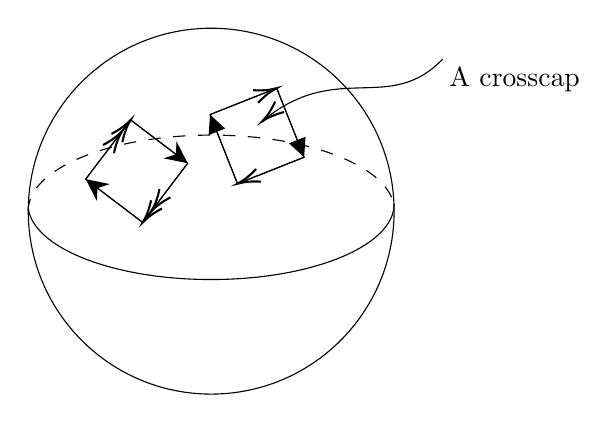
\begin{tikzpicture}[x=0.75pt,y=0.75pt,yscale=-1,xscale=1]
				%uncomment if require: \path (0,300); %set diagram left start at 0, and has height of 300
				
				%Shape: Ellipse [id:dp6864336997996399] 
				\draw   (221.04,171.13) .. controls (221.04,122.46) and (260.5,83) .. (309.17,83) .. controls (357.85,83) and (397.3,122.46) .. (397.3,171.13) .. controls (397.3,219.81) and (357.85,259.27) .. (309.17,259.27) .. controls (260.5,259.27) and (221.04,219.81) .. (221.04,171.13) -- cycle ;
				%Shape: Arc [id:dp7281461658543601] 
				\draw  [draw opacity=0] (397.3,167.44) .. controls (397.3,167.55) and (397.3,167.66) .. (397.3,167.78) .. controls (397.3,187.83) and (357.82,204.08) .. (309.11,204.08) .. controls (261.92,204.08) and (223.39,188.82) .. (221.04,169.64) -- (309.11,167.78) -- cycle ; \draw   (397.3,167.44) .. controls (397.3,167.55) and (397.3,167.66) .. (397.3,167.78) .. controls (397.3,187.83) and (357.82,204.08) .. (309.11,204.08) .. controls (261.92,204.08) and (223.39,188.82) .. (221.04,169.64) ;
				%Shape: Arc [id:dp8334402078144221] 
				\draw  [draw opacity=0][dash pattern={on 4.5pt off 4.5pt}] (221.04,171.13) .. controls (221.04,171.02) and (221.03,170.91) .. (221.03,170.79) .. controls (221.03,150.75) and (260.52,134.49) .. (309.23,134.49) .. controls (356.42,134.49) and (394.95,149.75) .. (397.3,168.93) -- (309.23,170.79) -- cycle ; \draw  [dash pattern={on 4.5pt off 4.5pt}] (221.04,171.13) .. controls (221.04,171.02) and (221.03,170.91) .. (221.03,170.79) .. controls (221.03,150.75) and (260.52,134.49) .. (309.23,134.49) .. controls (356.42,134.49) and (394.95,149.75) .. (397.3,168.93) ;
				%Shape: Rectangle [id:dp19102675121627555] 
				\draw   (308.63,124.61) -- (340.73,111.87) -- (353.95,145.16) -- (321.85,157.9) -- cycle ;
				%Shape: Rectangle [id:dp8798142665065305] 
				\draw   (270.36,127.18) -- (297.87,148.05) -- (276.22,176.59) -- (248.71,155.71) -- cycle ;
				%Straight Lines [id:da9288730371156004] 
				\draw    (308.63,124.61) -- (338.87,112.6) ;
				\draw [shift={(340.73,111.87)}, rotate = 518.35] [color={rgb, 255:red, 0; green, 0; blue, 0 }  ][line width=0.75]    (10.93,-3.29) .. controls (6.95,-1.4) and (3.31,-0.3) .. (0,0) .. controls (3.31,0.3) and (6.95,1.4) .. (10.93,3.29)   ;
				%Straight Lines [id:da4769536660684168] 
				\draw    (353.95,145.16) -- (323.71,157.16) ;
				\draw [shift={(321.85,157.9)}, rotate = 338.35] [color={rgb, 255:red, 0; green, 0; blue, 0 }  ][line width=0.75]    (10.93,-3.29) .. controls (6.95,-1.4) and (3.31,-0.3) .. (0,0) .. controls (3.31,0.3) and (6.95,1.4) .. (10.93,3.29)   ;
				%Straight Lines [id:da15681785837170215] 
				\draw    (321.85,157.9) -- (309.74,127.4) ;
				\draw [shift={(308.63,124.61)}, rotate = 428.35] [fill={rgb, 255:red, 0; green, 0; blue, 0 }  ][line width=0.08]  [draw opacity=0] (8.93,-4.29) -- (0,0) -- (8.93,4.29) -- cycle    ;
				%Straight Lines [id:da8620954353264538] 
				\draw    (340.73,111.87) -- (352.84,142.37) ;
				\draw [shift={(353.95,145.16)}, rotate = 248.35] [fill={rgb, 255:red, 0; green, 0; blue, 0 }  ][line width=0.08]  [draw opacity=0] (8.93,-4.29) -- (0,0) -- (8.93,4.29) -- cycle    ;
				%Straight Lines [id:da2852882406991285] 
				\draw    (248.71,155.71) -- (270.36,127.18) ;
				\draw [shift={(270.36,127.18)}, rotate = 487.19] [color={rgb, 255:red, 0; green, 0; blue, 0 }  ][line width=0.75]    (17.64,-3.29) .. controls (13.66,-1.4) and (10.02,-0.3) .. (6.71,0) .. controls (10.02,0.3) and (13.66,1.4) .. (17.64,3.29)(10.93,-3.29) .. controls (6.95,-1.4) and (3.31,-0.3) .. (0,0) .. controls (3.31,0.3) and (6.95,1.4) .. (10.93,3.29)   ;
				%Straight Lines [id:da9547130146841868] 
				\draw    (297.87,148.05) -- (276.22,176.59) ;
				\draw [shift={(276.22,176.59)}, rotate = 307.19] [color={rgb, 255:red, 0; green, 0; blue, 0 }  ][line width=0.75]    (17.64,-3.29) .. controls (13.66,-1.4) and (10.02,-0.3) .. (6.71,0) .. controls (10.02,0.3) and (13.66,1.4) .. (17.64,3.29)(10.93,-3.29) .. controls (6.95,-1.4) and (3.31,-0.3) .. (0,0) .. controls (3.31,0.3) and (6.95,1.4) .. (10.93,3.29)   ;
				%Straight Lines [id:da48489706469234506] 
				\draw    (276.22,176.59) -- (251.1,157.53) ;
				\draw [shift={(248.71,155.71)}, rotate = 397.19] [fill={rgb, 255:red, 0; green, 0; blue, 0 }  ][line width=0.08]  [draw opacity=0] (10.72,-5.15) -- (0,0) -- (10.72,5.15) -- (7.12,0) -- cycle    ;
				%Straight Lines [id:da9230569931037013] 
				\draw    (270.36,127.18) -- (295.48,146.24) ;
				\draw [shift={(297.87,148.05)}, rotate = 217.19] [fill={rgb, 255:red, 0; green, 0; blue, 0 }  ][line width=0.08]  [draw opacity=0] (10.72,-5.15) -- (0,0) -- (10.72,5.15) -- (7.12,0) -- cycle    ;
				%Curve Lines [id:da9205364076484657] 
				\draw    (420.73,97.87) .. controls (394.99,124.6) and (370.23,98.4) .. (334.81,126.98) ;
				\draw [shift={(333.73,127.87)}, rotate = 320.19] [color={rgb, 255:red, 0; green, 0; blue, 0 }  ][line width=0.75]    (10.93,-3.29) .. controls (6.95,-1.4) and (3.31,-0.3) .. (0,0) .. controls (3.31,0.3) and (6.95,1.4) .. (10.93,3.29)   ;
				
				% Text Node
				\draw (422.73,100.87) node [anchor=north west][inner sep=0.75pt]   [align=left] {A crosscap};
				
				
				\end{tikzpicture}
				
			\end{center}
		
		To think directly, the q crosscap can be viewed as:
			\begin{equation*}
			\begin{aligned}
				\text{CrossCap}_q=S^2\#\underbrace{\mathbb{R}P^2\#\cdots\#\mathbb{R}P^2}_q
			\end{aligned}
			\end{equation*}
		 
		 We know:
		 	\begin{equation*}
		 	\begin{aligned}
		 		&\chi(x\# y)=\chi(x)+\chi(y)-2\\
		 		\Rightarrow &\chi(\text{CrossCap}_q)=2+1\times q-2\times q=2-q
		 	\end{aligned}
		 	\end{equation*}
		 
		We can also think this question geometrically. We know that a sphere with $\mathbb{R}P^2$ can be got by blowing a bubble :
			\begin{center}
				
				
				% Gradient Info
				
				\tikzset {_px4edmw83/.code = {\pgfsetadditionalshadetransform{ \pgftransformshift{\pgfpoint{0 bp } { 0 bp }  }  \pgftransformrotate{-135 }  \pgftransformscale{2 }  }}}
				\pgfdeclarehorizontalshading{_gt86htbkw}{150bp}{rgb(0bp)=(0.82,0.89,0.97);
					rgb(37.5bp)=(0.82,0.89,0.97);
					rgb(43.5bp)=(0.45,0.69,0.91);
					rgb(50.04761832101005bp)=(0.29,0.56,0.89);
					rgb(57.25bp)=(0.33,0.62,0.88);
					rgb(62.5bp)=(0.53,0.74,0.92);
					rgb(100bp)=(0.53,0.74,0.92)}
				\tikzset{_w69p2vl8z/.code = {\pgfsetadditionalshadetransform{\pgftransformshift{\pgfpoint{0 bp } { 0 bp }  }  \pgftransformrotate{-135 }  \pgftransformscale{2 } }}}
				\pgfdeclarehorizontalshading{_seu1t5mbp} {150bp} {color(0bp)=(transparent!0);
					color(37.5bp)=(transparent!0);
					color(43.5bp)=(transparent!0);
					color(50.04761832101005bp)=(transparent!26);
					color(57.25bp)=(transparent!0);
					color(62.5bp)=(transparent!0);
					color(100bp)=(transparent!0) } 
				\pgfdeclarefading{_5zxvbazt9}{\tikz \fill[shading=_seu1t5mbp,_w69p2vl8z] (0,0) rectangle (50bp,50bp); } 
				
				% Gradient Info
				
				\tikzset {_piba3uv59/.code = {\pgfsetadditionalshadetransform{ \pgftransformshift{\pgfpoint{0 bp } { 0 bp }  }  \pgftransformrotate{-135 }  \pgftransformscale{2 }  }}}
				\pgfdeclarehorizontalshading{_c2lokihh0}{150bp}{rgb(0bp)=(0.82,0.89,0.97);
					rgb(37.5bp)=(0.82,0.89,0.97);
					rgb(43.5bp)=(0.45,0.69,0.91);
					rgb(50bp)=(0.29,0.56,0.89);
					rgb(57.25bp)=(0.33,0.62,0.88);
					rgb(62.5bp)=(0.53,0.74,0.92);
					rgb(100bp)=(0.53,0.74,0.92)}
				\tikzset{_67dmx3920/.code = {\pgfsetadditionalshadetransform{\pgftransformshift{\pgfpoint{0 bp } { 0 bp }  }  \pgftransformrotate{-135 }  \pgftransformscale{2 } }}}
				\pgfdeclarehorizontalshading{_eqwo2ccbx} {150bp} {color(0bp)=(transparent!0);
					color(37.5bp)=(transparent!0);
					color(43.5bp)=(transparent!0);
					color(50bp)=(transparent!24);
					color(57.25bp)=(transparent!0);
					color(62.5bp)=(transparent!0);
					color(100bp)=(transparent!0) } 
				\pgfdeclarefading{_k8ov2a1s2}{\tikz \fill[shading=_eqwo2ccbx,_67dmx3920] (0,0) rectangle (50bp,50bp); } 
				\tikzset{every picture/.style={line width=0.75pt}} %set default line width to 0.75pt        
				
				\begin{tikzpicture}[x=0.75pt,y=0.75pt,yscale=-1,xscale=1]
				%uncomment if require: \path (0,300); %set diagram left start at 0, and has height of 300
				
				%Shape: Square [id:dp25331052537691956] 
				\path  [shading=_gt86htbkw,_px4edmw83,path fading= _5zxvbazt9 ,fading transform={xshift=2}] (126.53,112.02) -- (190.53,112.02) -- (190.53,176.02) -- (126.53,176.02) -- cycle ; % for fading 
				\draw   (126.53,112.02) -- (190.53,112.02) -- (190.53,176.02) -- (126.53,176.02) -- cycle ; % for border 
				
				%Straight Lines [id:da7187451150536516] 
				\draw    (128.88,112.02) -- (188.53,112.02) ;
				\draw [shift={(190.53,112.02)}, rotate = 180] [color={rgb, 255:red, 0; green, 0; blue, 0 }  ][line width=0.75]    (10.93,-3.29) .. controls (6.95,-1.4) and (3.31,-0.3) .. (0,0) .. controls (3.31,0.3) and (6.95,1.4) .. (10.93,3.29)   ;
				\draw [shift={(126.53,112.02)}, rotate = 0] [color={rgb, 255:red, 0; green, 0; blue, 0 }  ][line width=0.75]      (0, 0) circle [x radius= 3.35, y radius= 3.35]   ;
				%Straight Lines [id:da4591591059004253] 
				\draw    (188.18,176.02) -- (128.53,176.02) ;
				\draw [shift={(126.53,176.02)}, rotate = 360] [color={rgb, 255:red, 0; green, 0; blue, 0 }  ][line width=0.75]    (10.93,-3.29) .. controls (6.95,-1.4) and (3.31,-0.3) .. (0,0) .. controls (3.31,0.3) and (6.95,1.4) .. (10.93,3.29)   ;
				\draw [shift={(190.53,176.02)}, rotate = 180] [color={rgb, 255:red, 0; green, 0; blue, 0 }  ][line width=0.75]      (0, 0) circle [x radius= 3.35, y radius= 3.35]   ;
				%Straight Lines [id:da6701569253093812] 
				\draw    (126.53,176.02) -- (126.53,115.02) ;
				\draw [shift={(126.53,112.02)}, rotate = 450] [fill={rgb, 255:red, 0; green, 0; blue, 0 }  ][line width=0.08]  [draw opacity=0] (8.93,-4.29) -- (0,0) -- (8.93,4.29) -- cycle    ;
				\draw [shift={(126.53,176.02)}, rotate = 270] [color={rgb, 255:red, 0; green, 0; blue, 0 }  ][fill={rgb, 255:red, 0; green, 0; blue, 0 }  ][line width=0.75]      (0, 0) circle [x radius= 3.35, y radius= 3.35]   ;
				%Straight Lines [id:da9353812244063806] 
				\draw    (190.53,112.02) -- (190.53,173.02) ;
				\draw [shift={(190.53,176.02)}, rotate = 270] [fill={rgb, 255:red, 0; green, 0; blue, 0 }  ][line width=0.08]  [draw opacity=0] (8.93,-4.29) -- (0,0) -- (8.93,4.29) -- cycle    ;
				\draw [shift={(190.53,112.02)}, rotate = 90] [color={rgb, 255:red, 0; green, 0; blue, 0 }  ][fill={rgb, 255:red, 0; green, 0; blue, 0 }  ][line width=0.75]      (0, 0) circle [x radius= 3.35, y radius= 3.35]   ;
				%Shape: Ellipse [id:dp8657158131075344] 
				\path  [shading=_c2lokihh0,_piba3uv59,path fading= _k8ov2a1s2 ,fading transform={xshift=2}] (351.04,144.13) .. controls (351.04,95.46) and (390.5,56) .. (439.17,56) .. controls (487.85,56) and (527.3,95.46) .. (527.3,144.13) .. controls (527.3,192.81) and (487.85,232.27) .. (439.17,232.27) .. controls (390.5,232.27) and (351.04,192.81) .. (351.04,144.13) -- cycle ; % for fading 
				\draw   (351.04,144.13) .. controls (351.04,95.46) and (390.5,56) .. (439.17,56) .. controls (487.85,56) and (527.3,95.46) .. (527.3,144.13) .. controls (527.3,192.81) and (487.85,232.27) .. (439.17,232.27) .. controls (390.5,232.27) and (351.04,192.81) .. (351.04,144.13) -- cycle ; % for border 
				
				%Shape: Arc [id:dp43818838774969193] 
				\draw  [draw opacity=0] (527.3,140.44) .. controls (527.3,140.55) and (527.3,140.66) .. (527.3,140.78) .. controls (527.3,160.83) and (487.82,177.08) .. (439.11,177.08) .. controls (391.92,177.08) and (353.39,161.82) .. (351.04,142.64) -- (439.11,140.78) -- cycle ; \draw   (527.3,140.44) .. controls (527.3,140.55) and (527.3,140.66) .. (527.3,140.78) .. controls (527.3,160.83) and (487.82,177.08) .. (439.11,177.08) .. controls (391.92,177.08) and (353.39,161.82) .. (351.04,142.64) ;
				%Shape: Arc [id:dp6116023553792455] 
				\draw  [draw opacity=0][dash pattern={on 4.5pt off 4.5pt}] (351.04,144.13) .. controls (351.04,144.02) and (351.03,143.91) .. (351.03,143.79) .. controls (351.03,123.75) and (390.52,107.49) .. (439.23,107.49) .. controls (486.42,107.49) and (524.95,122.75) .. (527.3,141.93) -- (439.23,143.79) -- cycle ; \draw  [dash pattern={on 4.5pt off 4.5pt}] (351.04,144.13) .. controls (351.04,144.02) and (351.03,143.91) .. (351.03,143.79) .. controls (351.03,123.75) and (390.52,107.49) .. (439.23,107.49) .. controls (486.42,107.49) and (524.95,122.75) .. (527.3,141.93) ;
				%Shape: Rectangle [id:dp7809292216358654] 
				\draw  [fill={rgb, 255:red, 255; green, 255; blue, 255 }  ,fill opacity=1 ] (438.63,97.61) -- (470.73,84.87) -- (483.95,118.16) -- (451.85,130.9) -- cycle ;
				%Straight Lines [id:da9092821130019881] 
				\draw    (440.82,96.74) -- (468.87,85.6) ;
				\draw [shift={(470.73,84.87)}, rotate = 518.35] [color={rgb, 255:red, 0; green, 0; blue, 0 }  ][line width=0.75]    (10.93,-3.29) .. controls (6.95,-1.4) and (3.31,-0.3) .. (0,0) .. controls (3.31,0.3) and (6.95,1.4) .. (10.93,3.29)   ;
				\draw [shift={(438.63,97.61)}, rotate = 338.35] [color={rgb, 255:red, 0; green, 0; blue, 0 }  ][line width=0.75]      (0, 0) circle [x radius= 3.35, y radius= 3.35]   ;
				%Straight Lines [id:da10766434986608386] 
				\draw    (481.76,119.03) -- (453.71,130.16) ;
				\draw [shift={(451.85,130.9)}, rotate = 338.35] [color={rgb, 255:red, 0; green, 0; blue, 0 }  ][line width=0.75]    (10.93,-3.29) .. controls (6.95,-1.4) and (3.31,-0.3) .. (0,0) .. controls (3.31,0.3) and (6.95,1.4) .. (10.93,3.29)   ;
				\draw [shift={(483.95,118.16)}, rotate = 158.35] [color={rgb, 255:red, 0; green, 0; blue, 0 }  ][line width=0.75]      (0, 0) circle [x radius= 3.35, y radius= 3.35]   ;
				%Straight Lines [id:da4031184959426213] 
				\draw    (451.85,130.9) -- (439.74,100.4) ;
				\draw [shift={(438.63,97.61)}, rotate = 428.35] [fill={rgb, 255:red, 0; green, 0; blue, 0 }  ][line width=0.08]  [draw opacity=0] (8.93,-4.29) -- (0,0) -- (8.93,4.29) -- cycle    ;
				\draw [shift={(451.85,130.9)}, rotate = 248.35] [color={rgb, 255:red, 0; green, 0; blue, 0 }  ][fill={rgb, 255:red, 0; green, 0; blue, 0 }  ][line width=0.75]      (0, 0) circle [x radius= 3.35, y radius= 3.35]   ;
				%Straight Lines [id:da34114166449587235] 
				\draw    (470.73,84.87) -- (482.84,115.37) ;
				\draw [shift={(483.95,118.16)}, rotate = 248.35] [fill={rgb, 255:red, 0; green, 0; blue, 0 }  ][line width=0.08]  [draw opacity=0] (8.93,-4.29) -- (0,0) -- (8.93,4.29) -- cycle    ;
				\draw [shift={(470.73,84.87)}, rotate = 68.35] [color={rgb, 255:red, 0; green, 0; blue, 0 }  ][fill={rgb, 255:red, 0; green, 0; blue, 0 }  ][line width=0.75]      (0, 0) circle [x radius= 3.35, y radius= 3.35]   ;
				%Curve Lines [id:da04753674976986988] 
				\draw    (226,144) .. controls (265.6,114.3) and (285.6,172.81) .. (324.81,144.87) ;
				\draw [shift={(326,144)}, rotate = 503.13] [color={rgb, 255:red, 0; green, 0; blue, 0 }  ][line width=0.75]    (10.93,-3.29) .. controls (6.95,-1.4) and (3.31,-0.3) .. (0,0) .. controls (3.31,0.3) and (6.95,1.4) .. (10.93,3.29)   ;
				
				% Text Node
				\draw (233,116) node [anchor=north west][inner sep=0.75pt]   [align=left] {Blow bubble};
				
				
				\end{tikzpicture}
				
			\end{center}
		
		So inversely, we can get the trangulation of $q$ crosscap by inhaling the sphere: 
			\begin{center}
				
				
				% Gradient Info
				
				\tikzset {_parmy627k/.code = {\pgfsetadditionalshadetransform{ \pgftransformshift{\pgfpoint{0 bp } { 0 bp }  }  \pgftransformrotate{-135 }  \pgftransformscale{2 }  }}}
				\pgfdeclarehorizontalshading{_cx76b3erp}{150bp}{rgb(0bp)=(0.82,0.89,0.97);
					rgb(37.5bp)=(0.82,0.89,0.97);
					rgb(43.5bp)=(0.45,0.69,0.91);
					rgb(50bp)=(0.29,0.56,0.89);
					rgb(57.25bp)=(0.33,0.62,0.88);
					rgb(62.5bp)=(0.53,0.74,0.92);
					rgb(100bp)=(0.53,0.74,0.92)}
				\tikzset{_cl1qlc7ln/.code = {\pgfsetadditionalshadetransform{\pgftransformshift{\pgfpoint{0 bp } { 0 bp }  }  \pgftransformrotate{-135 }  \pgftransformscale{2 } }}}
				\pgfdeclarehorizontalshading{_uhig28e04} {150bp} {color(0bp)=(transparent!0);
					color(37.5bp)=(transparent!0);
					color(43.5bp)=(transparent!0);
					color(50bp)=(transparent!24);
					color(57.25bp)=(transparent!0);
					color(62.5bp)=(transparent!0);
					color(100bp)=(transparent!0) } 
				\pgfdeclarefading{_6i1h3tuo9}{\tikz \fill[shading=_uhig28e04,_cl1qlc7ln] (0,0) rectangle (50bp,50bp); } 
				
				% Gradient Info
				
				\tikzset {_19puxwjnv/.code = {\pgfsetadditionalshadetransform{ \pgftransformshift{\pgfpoint{0 bp } { 0 bp }  }  \pgftransformrotate{-135 }  \pgftransformscale{2 }  }}}
				\pgfdeclarehorizontalshading{_k5hkxsw69}{150bp}{rgb(0bp)=(0.82,0.89,0.97);
					rgb(37.5bp)=(0.82,0.89,0.97);
					rgb(43.5bp)=(0.45,0.69,0.91);
					rgb(50.04761832101005bp)=(0.29,0.56,0.89);
					rgb(57.25bp)=(0.33,0.62,0.88);
					rgb(62.5bp)=(0.53,0.74,0.92);
					rgb(100bp)=(0.53,0.74,0.92)}
				\tikzset{_a76ax7ngj/.code = {\pgfsetadditionalshadetransform{\pgftransformshift{\pgfpoint{0 bp } { 0 bp }  }  \pgftransformrotate{-135 }  \pgftransformscale{2 } }}}
				\pgfdeclarehorizontalshading{_366a313v2} {150bp} {color(0bp)=(transparent!0);
					color(37.5bp)=(transparent!0);
					color(43.5bp)=(transparent!0);
					color(50.04761832101005bp)=(transparent!26);
					color(57.25bp)=(transparent!0);
					color(62.5bp)=(transparent!0);
					color(100bp)=(transparent!0) } 
				\pgfdeclarefading{_ck4o0mqvj}{\tikz \fill[shading=_366a313v2,_a76ax7ngj] (0,0) rectangle (50bp,50bp); } 
				\tikzset{every picture/.style={line width=0.75pt}} %set default line width to 0.75pt        
				
				\begin{tikzpicture}[x=0.75pt,y=0.75pt,yscale=-1,xscale=1]
				%uncomment if require: \path (0,300); %set diagram left start at 0, and has height of 300
				
				%Shape: Ellipse [id:dp32296844890676313] 
				\path  [shading=_cx76b3erp,_parmy627k,path fading= _6i1h3tuo9 ,fading transform={xshift=2}] (89.04,143.13) .. controls (89.04,94.46) and (128.5,55) .. (177.17,55) .. controls (225.85,55) and (265.3,94.46) .. (265.3,143.13) .. controls (265.3,191.81) and (225.85,231.27) .. (177.17,231.27) .. controls (128.5,231.27) and (89.04,191.81) .. (89.04,143.13) -- cycle ; % for fading 
				\draw   (89.04,143.13) .. controls (89.04,94.46) and (128.5,55) .. (177.17,55) .. controls (225.85,55) and (265.3,94.46) .. (265.3,143.13) .. controls (265.3,191.81) and (225.85,231.27) .. (177.17,231.27) .. controls (128.5,231.27) and (89.04,191.81) .. (89.04,143.13) -- cycle ; % for border 
				
				%Shape: Rectangle [id:dp2719208025355515] 
				\draw  [fill={rgb, 255:red, 255; green, 255; blue, 255 }  ,fill opacity=1 ] (140.36,91.64) -- (167.87,112.52) -- (146.22,141.06) -- (118.71,120.18) -- cycle ;
				%Straight Lines [id:da9769874974827132] 
				\draw    (120.13,118.31) -- (140.36,91.64) ;
				\draw [shift={(140.36,91.64)}, rotate = 487.19] [color={rgb, 255:red, 0; green, 0; blue, 0 }  ][line width=0.75]    (17.64,-3.29) .. controls (13.66,-1.4) and (10.02,-0.3) .. (6.71,0) .. controls (10.02,0.3) and (13.66,1.4) .. (17.64,3.29)(10.93,-3.29) .. controls (6.95,-1.4) and (3.31,-0.3) .. (0,0) .. controls (3.31,0.3) and (6.95,1.4) .. (10.93,3.29)   ;
				\draw [shift={(118.71,120.18)}, rotate = 307.19] [color={rgb, 255:red, 0; green, 0; blue, 0 }  ][line width=0.75]      (0, 0) circle [x radius= 3.35, y radius= 3.35]   ;
				%Straight Lines [id:da999032625921261] 
				\draw    (166.45,114.39) -- (146.22,141.06) ;
				\draw [shift={(146.22,141.06)}, rotate = 307.19] [color={rgb, 255:red, 0; green, 0; blue, 0 }  ][line width=0.75]    (17.64,-3.29) .. controls (13.66,-1.4) and (10.02,-0.3) .. (6.71,0) .. controls (10.02,0.3) and (13.66,1.4) .. (17.64,3.29)(10.93,-3.29) .. controls (6.95,-1.4) and (3.31,-0.3) .. (0,0) .. controls (3.31,0.3) and (6.95,1.4) .. (10.93,3.29)   ;
				\draw [shift={(167.87,112.52)}, rotate = 127.19] [color={rgb, 255:red, 0; green, 0; blue, 0 }  ][line width=0.75]      (0, 0) circle [x radius= 3.35, y radius= 3.35]   ;
				%Straight Lines [id:da8872149244505629] 
				\draw    (146.22,141.06) -- (121.1,121.99) ;
				\draw [shift={(118.71,120.18)}, rotate = 397.19] [fill={rgb, 255:red, 0; green, 0; blue, 0 }  ][line width=0.08]  [draw opacity=0] (10.72,-5.15) -- (0,0) -- (10.72,5.15) -- (7.12,0) -- cycle    ;
				\draw [shift={(146.22,141.06)}, rotate = 217.19] [color={rgb, 255:red, 0; green, 0; blue, 0 }  ][fill={rgb, 255:red, 0; green, 0; blue, 0 }  ][line width=0.75]      (0, 0) circle [x radius= 3.35, y radius= 3.35]   ;
				%Straight Lines [id:da03020758819728986] 
				\draw    (140.36,91.64) -- (165.48,110.71) ;
				\draw [shift={(167.87,112.52)}, rotate = 217.19] [fill={rgb, 255:red, 0; green, 0; blue, 0 }  ][line width=0.08]  [draw opacity=0] (10.72,-5.15) -- (0,0) -- (10.72,5.15) -- (7.12,0) -- cycle    ;
				\draw [shift={(140.36,91.64)}, rotate = 37.19] [color={rgb, 255:red, 0; green, 0; blue, 0 }  ][fill={rgb, 255:red, 0; green, 0; blue, 0 }  ][line width=0.75]      (0, 0) circle [x radius= 3.35, y radius= 3.35]   ;
				%Shape: Arc [id:dp5005182910807038] 
				\draw  [draw opacity=0] (265.3,139.44) .. controls (265.3,139.55) and (265.3,139.66) .. (265.3,139.78) .. controls (265.3,159.83) and (225.82,176.08) .. (177.11,176.08) .. controls (129.92,176.08) and (91.39,160.82) .. (89.04,141.64) -- (177.11,139.78) -- cycle ; \draw   (265.3,139.44) .. controls (265.3,139.55) and (265.3,139.66) .. (265.3,139.78) .. controls (265.3,159.83) and (225.82,176.08) .. (177.11,176.08) .. controls (129.92,176.08) and (91.39,160.82) .. (89.04,141.64) ;
				%Shape: Arc [id:dp45617051448423873] 
				\draw  [draw opacity=0][dash pattern={on 4.5pt off 4.5pt}] (89.04,143.13) .. controls (89.04,143.02) and (89.03,142.91) .. (89.03,142.79) .. controls (89.03,122.75) and (128.52,106.49) .. (177.23,106.49) .. controls (224.42,106.49) and (262.95,121.75) .. (265.3,140.93) -- (177.23,142.79) -- cycle ; \draw  [dash pattern={on 4.5pt off 4.5pt}] (89.04,143.13) .. controls (89.04,143.02) and (89.03,142.91) .. (89.03,142.79) .. controls (89.03,122.75) and (128.52,106.49) .. (177.23,106.49) .. controls (224.42,106.49) and (262.95,121.75) .. (265.3,140.93) ;
				%Shape: Rectangle [id:dp197252005749184] 
				\draw  [fill={rgb, 255:red, 255; green, 255; blue, 255 }  ,fill opacity=1 ] (176.63,96.61) -- (208.73,83.87) -- (221.95,117.16) -- (189.85,129.9) -- cycle ;
				%Straight Lines [id:da6318400184634119] 
				\draw    (178.82,95.74) -- (206.87,84.6) ;
				\draw [shift={(208.73,83.87)}, rotate = 518.35] [color={rgb, 255:red, 0; green, 0; blue, 0 }  ][line width=0.75]    (10.93,-3.29) .. controls (6.95,-1.4) and (3.31,-0.3) .. (0,0) .. controls (3.31,0.3) and (6.95,1.4) .. (10.93,3.29)   ;
				\draw [shift={(176.63,96.61)}, rotate = 338.35] [color={rgb, 255:red, 0; green, 0; blue, 0 }  ][line width=0.75]      (0, 0) circle [x radius= 3.35, y radius= 3.35]   ;
				%Straight Lines [id:da6921011626415812] 
				\draw    (219.76,118.03) -- (191.71,129.16) ;
				\draw [shift={(189.85,129.9)}, rotate = 338.35] [color={rgb, 255:red, 0; green, 0; blue, 0 }  ][line width=0.75]    (10.93,-3.29) .. controls (6.95,-1.4) and (3.31,-0.3) .. (0,0) .. controls (3.31,0.3) and (6.95,1.4) .. (10.93,3.29)   ;
				\draw [shift={(221.95,117.16)}, rotate = 158.35] [color={rgb, 255:red, 0; green, 0; blue, 0 }  ][line width=0.75]      (0, 0) circle [x radius= 3.35, y radius= 3.35]   ;
				%Straight Lines [id:da8523247374716839] 
				\draw    (189.85,129.9) -- (177.74,99.4) ;
				\draw [shift={(176.63,96.61)}, rotate = 428.35] [fill={rgb, 255:red, 0; green, 0; blue, 0 }  ][line width=0.08]  [draw opacity=0] (8.93,-4.29) -- (0,0) -- (8.93,4.29) -- cycle    ;
				\draw [shift={(189.85,129.9)}, rotate = 248.35] [color={rgb, 255:red, 0; green, 0; blue, 0 }  ][fill={rgb, 255:red, 0; green, 0; blue, 0 }  ][line width=0.75]      (0, 0) circle [x radius= 3.35, y radius= 3.35]   ;
				%Straight Lines [id:da7543010486678514] 
				\draw    (208.73,83.87) -- (220.84,114.37) ;
				\draw [shift={(221.95,117.16)}, rotate = 248.35] [fill={rgb, 255:red, 0; green, 0; blue, 0 }  ][line width=0.08]  [draw opacity=0] (8.93,-4.29) -- (0,0) -- (8.93,4.29) -- cycle    ;
				\draw [shift={(208.73,83.87)}, rotate = 68.35] [color={rgb, 255:red, 0; green, 0; blue, 0 }  ][fill={rgb, 255:red, 0; green, 0; blue, 0 }  ][line width=0.75]      (0, 0) circle [x radius= 3.35, y radius= 3.35]   ;
				%Curve Lines [id:da16269439929642115] 
				\draw    (300,145) .. controls (339.6,115.3) and (359.6,173.81) .. (398.81,145.87) ;
				\draw [shift={(400,145)}, rotate = 503.13] [color={rgb, 255:red, 0; green, 0; blue, 0 }  ][line width=0.75]    (10.93,-3.29) .. controls (6.95,-1.4) and (3.31,-0.3) .. (0,0) .. controls (3.31,0.3) and (6.95,1.4) .. (10.93,3.29)   ;
				%Shape: Square [id:dp9651047073070218] 
				\path  [shading=_k5hkxsw69,_19puxwjnv,path fading= _ck4o0mqvj ,fading transform={xshift=2}] (466.53,104.02) -- (563.22,104.02) -- (563.22,200.7) -- (466.53,200.7) -- cycle ; % for fading 
				\draw   (466.53,104.02) -- (563.22,104.02) -- (563.22,200.7) -- (466.53,200.7) -- cycle ; % for border 
				
				%Straight Lines [id:da9141986879885856] 
				\draw    (468.88,104.02) -- (561.22,104.02) ;
				\draw [shift={(563.22,104.02)}, rotate = 180] [color={rgb, 255:red, 0; green, 0; blue, 0 }  ][line width=0.75]    (10.93,-3.29) .. controls (6.95,-1.4) and (3.31,-0.3) .. (0,0) .. controls (3.31,0.3) and (6.95,1.4) .. (10.93,3.29)   ;
				\draw [shift={(466.53,104.02)}, rotate = 0] [color={rgb, 255:red, 0; green, 0; blue, 0 }  ][line width=0.75]      (0, 0) circle [x radius= 3.35, y radius= 3.35]   ;
				%Straight Lines [id:da8717731460630849] 
				\draw    (560.87,200.7) -- (468.53,200.7) ;
				\draw [shift={(466.53,200.7)}, rotate = 360] [color={rgb, 255:red, 0; green, 0; blue, 0 }  ][line width=0.75]    (10.93,-3.29) .. controls (6.95,-1.4) and (3.31,-0.3) .. (0,0) .. controls (3.31,0.3) and (6.95,1.4) .. (10.93,3.29)   ;
				\draw [shift={(563.22,200.7)}, rotate = 180] [color={rgb, 255:red, 0; green, 0; blue, 0 }  ][line width=0.75]      (0, 0) circle [x radius= 3.35, y radius= 3.35]   ;
				%Straight Lines [id:da2860506982084988] 
				\draw    (466.53,200.7) -- (466.53,107.02) ;
				\draw [shift={(466.53,104.02)}, rotate = 450] [fill={rgb, 255:red, 0; green, 0; blue, 0 }  ][line width=0.08]  [draw opacity=0] (8.93,-4.29) -- (0,0) -- (8.93,4.29) -- cycle    ;
				\draw [shift={(466.53,200.7)}, rotate = 270] [color={rgb, 255:red, 0; green, 0; blue, 0 }  ][fill={rgb, 255:red, 0; green, 0; blue, 0 }  ][line width=0.75]      (0, 0) circle [x radius= 3.35, y radius= 3.35]   ;
				%Straight Lines [id:da6045175421008437] 
				\draw    (563.22,104.02) -- (563.22,197.7) ;
				\draw [shift={(563.22,200.7)}, rotate = 270] [fill={rgb, 255:red, 0; green, 0; blue, 0 }  ][line width=0.08]  [draw opacity=0] (8.93,-4.29) -- (0,0) -- (8.93,4.29) -- cycle    ;
				\draw [shift={(563.22,104.02)}, rotate = 90] [color={rgb, 255:red, 0; green, 0; blue, 0 }  ][fill={rgb, 255:red, 0; green, 0; blue, 0 }  ][line width=0.75]      (0, 0) circle [x radius= 3.35, y radius= 3.35]   ;
				%Shape: Square [id:dp31704441787678816] 
				\draw  [fill={rgb, 255:red, 255; green, 255; blue, 255 }  ,fill opacity=1 ] (489.88,127.36) -- (539.88,127.36) -- (539.88,177.36) -- (489.88,177.36) -- cycle ;
				%Straight Lines [id:da030366184660737705] 
				\draw    (489.88,177.36) -- (489.88,130.36) ;
				\draw [shift={(489.88,127.36)}, rotate = 450] [fill={rgb, 255:red, 0; green, 0; blue, 0 }  ][line width=0.08]  [draw opacity=0] (10.72,-5.15) -- (0,0) -- (10.72,5.15) -- (7.12,0) -- cycle    ;
				\draw [shift={(489.88,177.36)}, rotate = 270] [color={rgb, 255:red, 0; green, 0; blue, 0 }  ][fill={rgb, 255:red, 0; green, 0; blue, 0 }  ][line width=0.75]      (0, 0) circle [x radius= 3.35, y radius= 3.35]   ;
				%Straight Lines [id:da7652846867182466] 
				\draw    (492.23,127.36) -- (539.88,127.36) ;
				\draw [shift={(539.88,127.36)}, rotate = 180] [color={rgb, 255:red, 0; green, 0; blue, 0 }  ][line width=0.75]    (17.64,-3.29) .. controls (13.66,-1.4) and (10.02,-0.3) .. (6.71,0) .. controls (10.02,0.3) and (13.66,1.4) .. (17.64,3.29)(10.93,-3.29) .. controls (6.95,-1.4) and (3.31,-0.3) .. (0,0) .. controls (3.31,0.3) and (6.95,1.4) .. (10.93,3.29)   ;
				\draw [shift={(489.88,127.36)}, rotate = 0] [color={rgb, 255:red, 0; green, 0; blue, 0 }  ][line width=0.75]      (0, 0) circle [x radius= 3.35, y radius= 3.35]   ;
				%Straight Lines [id:da982493046963186] 
				\draw    (539.88,127.36) -- (539.88,174.36) ;
				\draw [shift={(539.88,177.36)}, rotate = 270] [fill={rgb, 255:red, 0; green, 0; blue, 0 }  ][line width=0.08]  [draw opacity=0] (10.72,-5.15) -- (0,0) -- (10.72,5.15) -- (7.12,0) -- cycle    ;
				\draw [shift={(539.88,127.36)}, rotate = 90] [color={rgb, 255:red, 0; green, 0; blue, 0 }  ][fill={rgb, 255:red, 0; green, 0; blue, 0 }  ][line width=0.75]      (0, 0) circle [x radius= 3.35, y radius= 3.35]   ;
				%Straight Lines [id:da9066661102751706] 
				\draw    (537.53,177.36) -- (489.88,177.36) ;
				\draw [shift={(489.88,177.36)}, rotate = 360] [color={rgb, 255:red, 0; green, 0; blue, 0 }  ][line width=0.75]    (17.64,-3.29) .. controls (13.66,-1.4) and (10.02,-0.3) .. (6.71,0) .. controls (10.02,0.3) and (13.66,1.4) .. (17.64,3.29)(10.93,-3.29) .. controls (6.95,-1.4) and (3.31,-0.3) .. (0,0) .. controls (3.31,0.3) and (6.95,1.4) .. (10.93,3.29)   ;
				\draw [shift={(539.88,177.36)}, rotate = 180] [color={rgb, 255:red, 0; green, 0; blue, 0 }  ][line width=0.75]      (0, 0) circle [x radius= 3.35, y radius= 3.35]   ;
				%Straight Lines [id:da4039586776071694] 
				\draw    (466.53,200.7) -- (489.88,177.36) ;
				\draw [shift={(489.88,177.36)}, rotate = 495] [color={rgb, 255:red, 0; green, 0; blue, 0 }  ][line width=0.75]      (5.59,-5.59) .. controls (2.5,-5.59) and (0,-3.09) .. (0,0) .. controls (0,3.09) and (2.5,5.59) .. (5.59,5.59) ;
				%Straight Lines [id:da4816036274717883] 
				\draw    (563.22,104.02) -- (539.88,127.36) ;
				\draw [shift={(539.88,127.36)}, rotate = 315] [color={rgb, 255:red, 0; green, 0; blue, 0 }  ][line width=0.75]      (5.59,-5.59) .. controls (2.5,-5.59) and (0,-3.09) .. (0,0) .. controls (0,3.09) and (2.5,5.59) .. (5.59,5.59) ;
				%Straight Lines [id:da10746644011690532] 
				\draw    (466.53,104.02) -- (489.88,127.36) ;
				\draw [shift={(489.88,127.36)}, rotate = 225] [color={rgb, 255:red, 0; green, 0; blue, 0 }  ][line width=0.75]    (0,5.59) -- (0,-5.59)   ;
				%Straight Lines [id:da9323981653696565] 
				\draw    (563.22,200.7) -- (539.88,177.36) ;
				\draw [shift={(539.88,177.36)}, rotate = 405] [color={rgb, 255:red, 0; green, 0; blue, 0 }  ][line width=0.75]    (0,5.59) -- (0,-5.59)   ;
				
				% Text Node
				\draw (307,117) node [anchor=north west][inner sep=0.75pt]   [align=left] {Inhale bubble};
				
				
				\end{tikzpicture}
				
			\end{center}
		
		So the Euler characteristic can be calculated by:
			\begin{equation*}
			\begin{aligned}
				&\chi(\text{CrossCap}_2)=2-6+4=0\\
				&\chi(\text{CrossCap}_q)=2-q
			\end{aligned}
			\end{equation*}
		
		You can also using the trick: CrossCap$\setminus$Disk=Mobius trip to think the result. 
			
	\subsection{Exercise 5.13}
		This is pretty interesting. The regular polyhedra is also called the \textbf{Platonic solid}, they first appeared in <Timaeus>, they are viewed as different element of the world(earth, air, water and fire). To prove there are only five, there are many different approaches. You can using elementary geometry to prove this statement, as greeks did. Here we use Euler' s theorem. We know for a regular polyhedron, the number of edges attach to every vertex is the same, we call it $q$, and call the number of edges on one faces $p$. Because every edge have two vertex and on two faces, we have:
			\begin{equation*}
			\begin{aligned}
			pF=2E=qV
			\end{aligned}
			\end{equation*}
		
		With Euler's formular:
			\begin{equation*}
			\begin{aligned}
				V-E+F=2
			\end{aligned}
			\end{equation*}
		
		We have:
			\begin{equation*}
			\begin{aligned}
				\begin{cases}
					V=\frac{4p}{4-(p-2)(q-2)}\\
					E=\frac{2pq}{4-(p-2)(q-2)}\\
					F=\frac{4q}{4-(p-2)(q-2)}
				\end{cases}
			\end{aligned}
			\end{equation*}
		
		And
			\begin{equation*}
			\begin{aligned}
				\frac{1}{q}+\frac{1}{p}=\frac{1}{2}+\frac{1}{E}>\frac{1}{2}
			\end{aligned}
			\end{equation*}
		
		With $p,q>3$, we can find all pairs of $(p,q)$:
			\begin{enumerate}
				\item $ (p,q)=(3,3), \Rightarrow F=\frac{4q}{4-(p-2)(q-2)}=4$, so it is the tetrahedron. 
				
				\begin{center}
					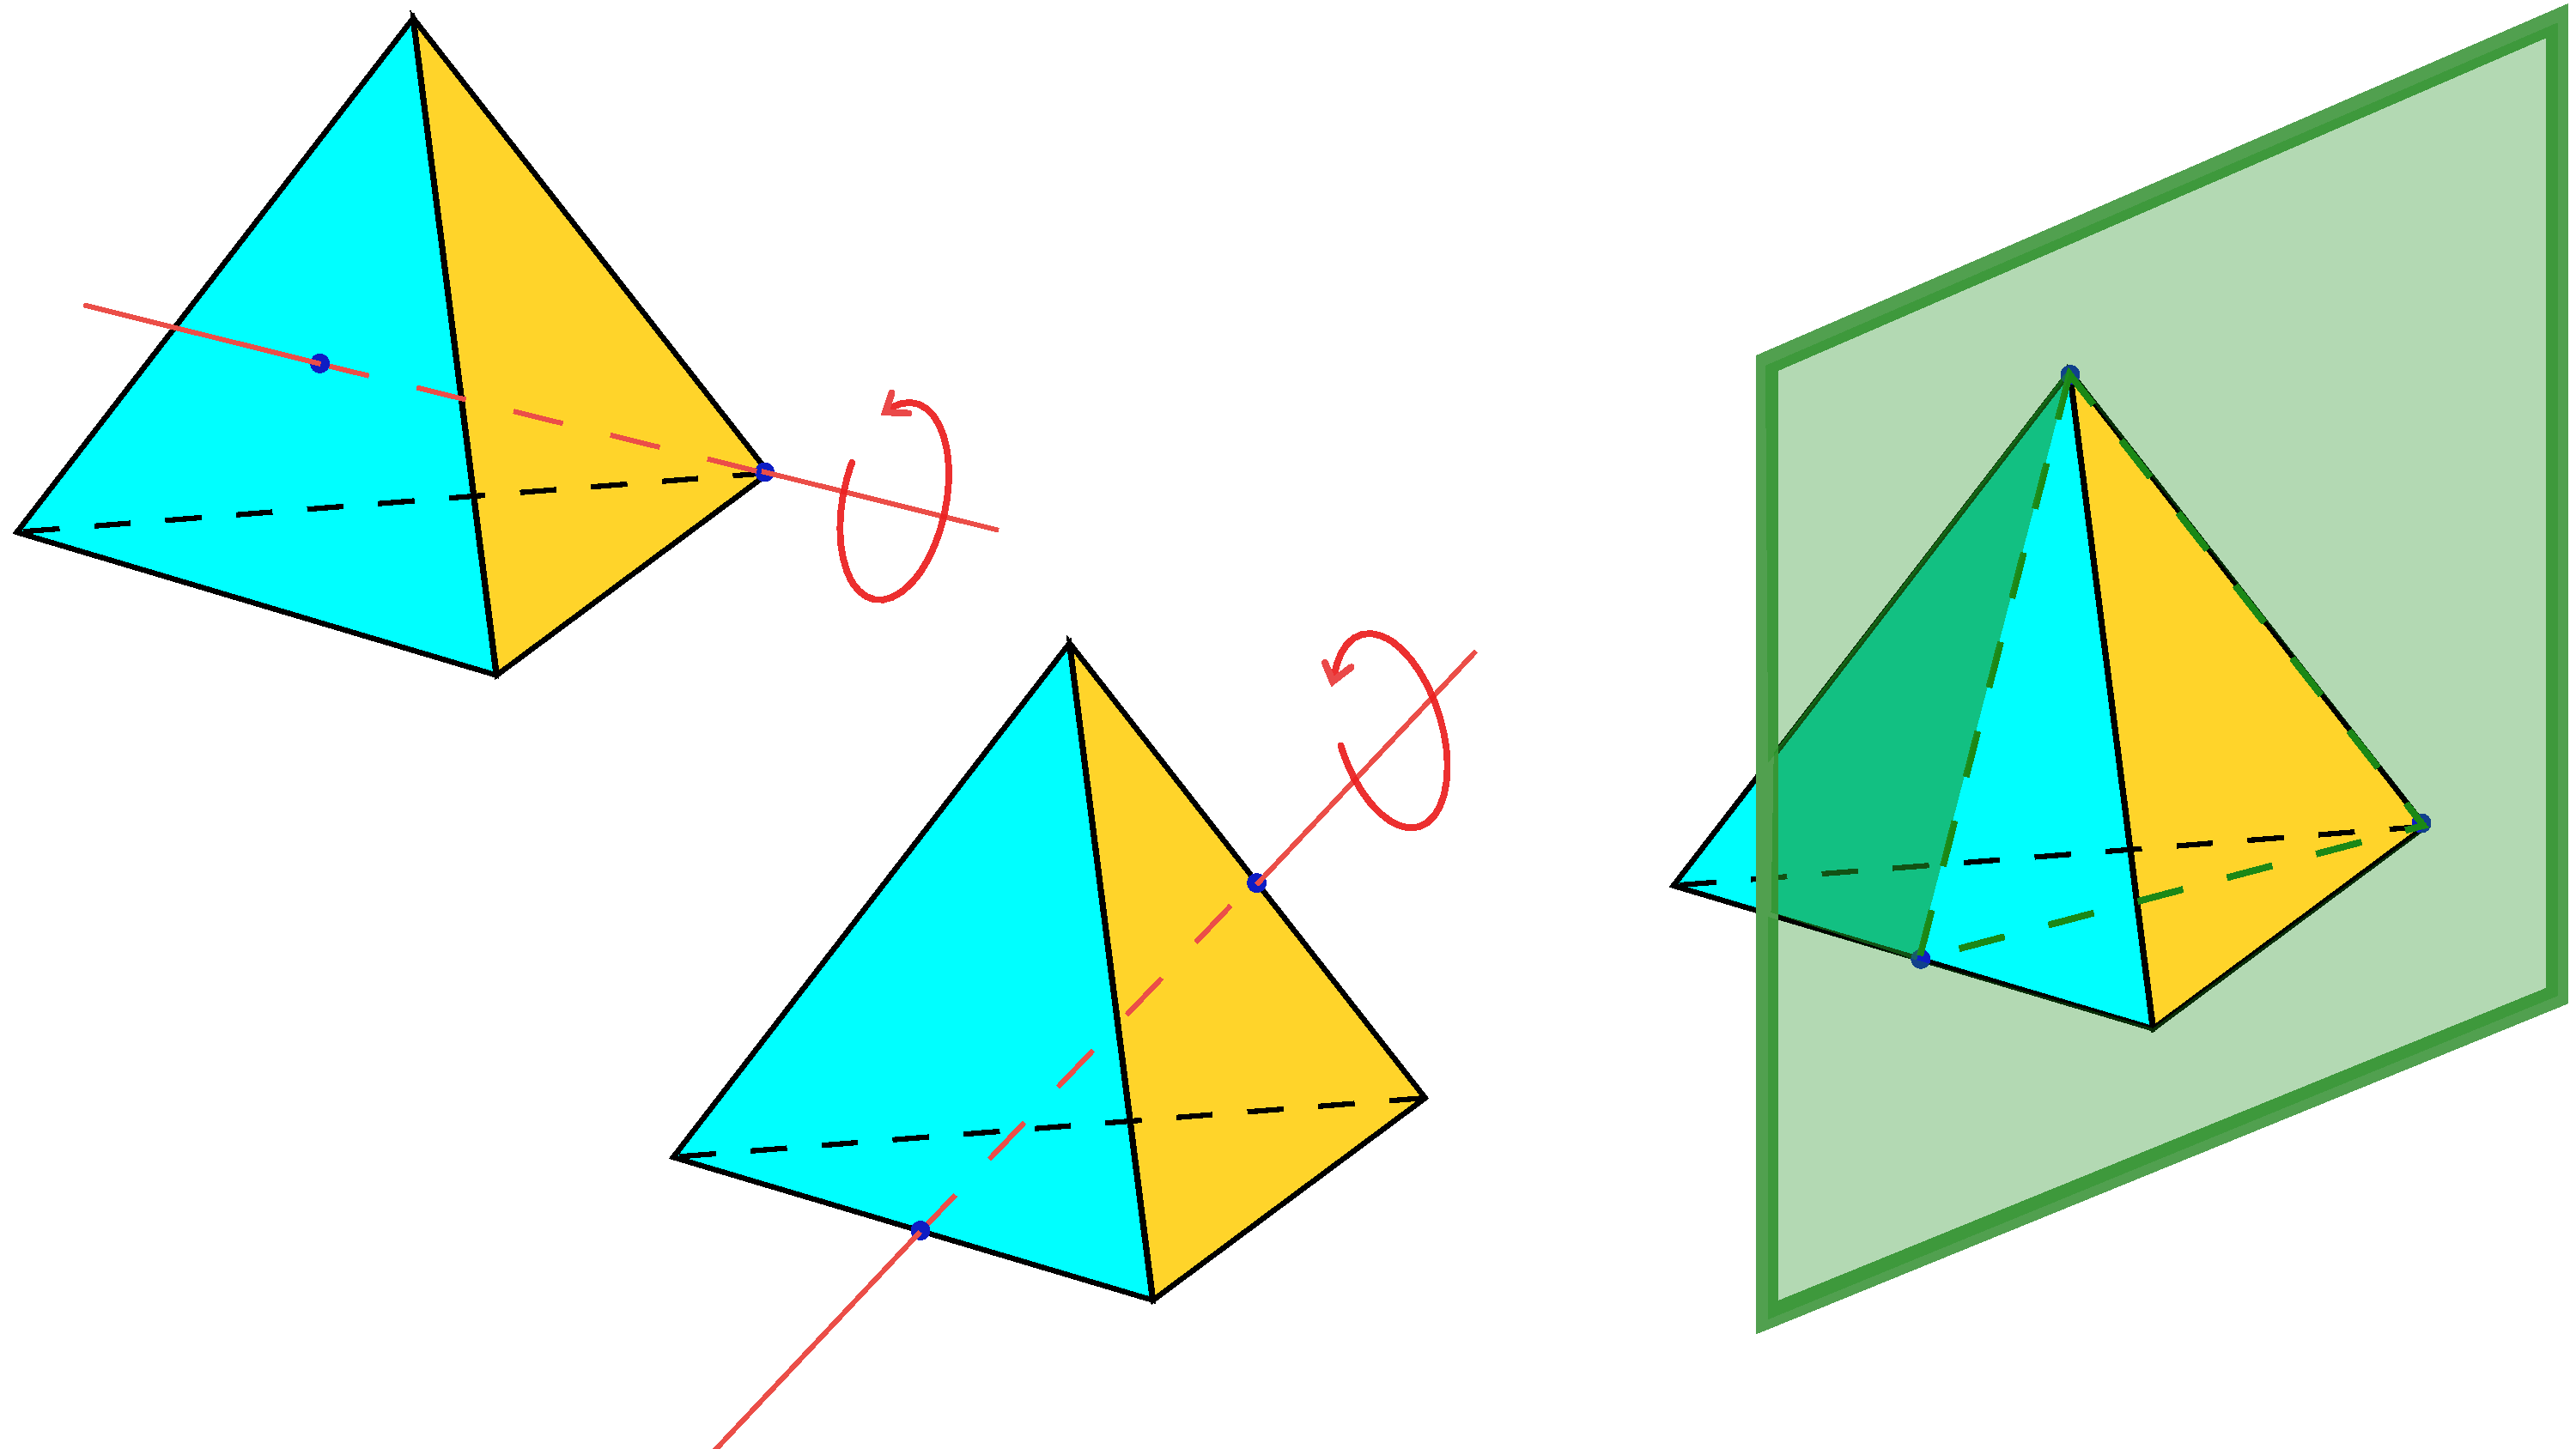
\includegraphics[scale=0.2]{Symmetries_of_the_tetrahedron.pdf}
				\end{center}
				\item $ (p,q)=(4,3), \Rightarrow F=\frac{4q}{4-(p-2)(q-2)}=6$, so it is the cube. 
				\item $ (p,q)=(3,4), \Rightarrow F=\frac{4q}{4-(p-2)(q-2)}=8$, so it is the octahedron.
				
				\begin{center}
					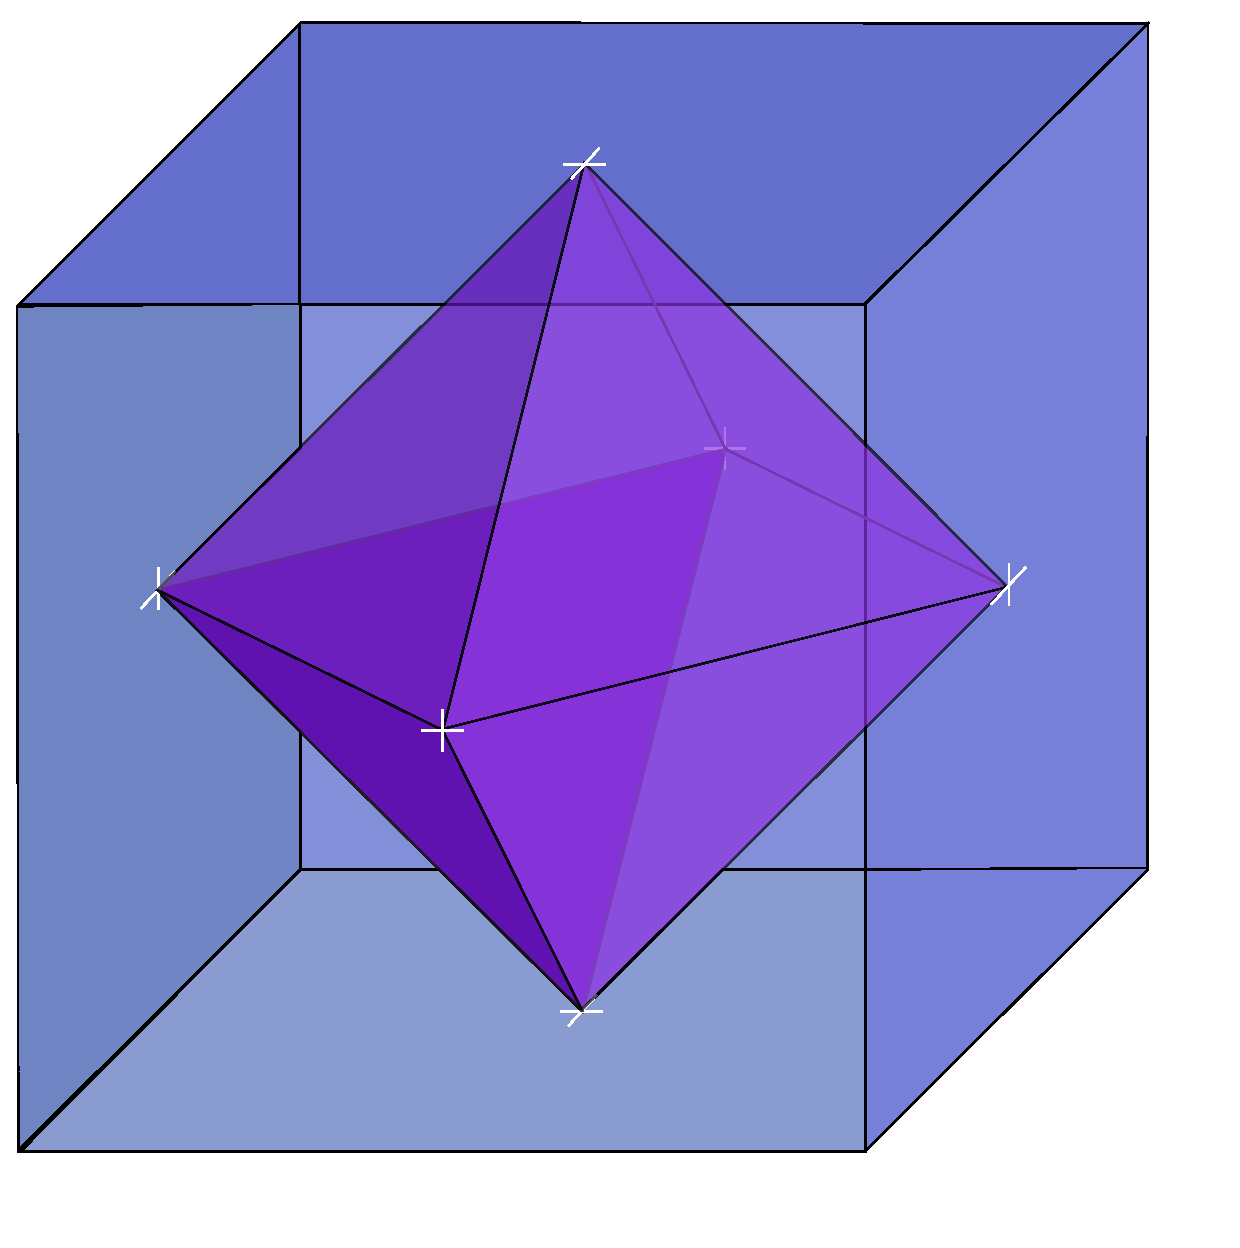
\includegraphics[scale=0.3]{Dual_Cube-Octahedron_1.pdf}
				\end{center}
				\item  $ (p,q)=(5,3), \Rightarrow F=\frac{4q}{4-(p-2)(q-2)}=12$, so it is the dodecahedron.
				
				\begin{center}
					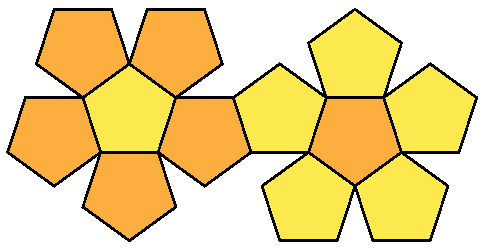
\includegraphics[scale=0.7]{Dodecahedron_flat_1.pdf}
				\end{center}
				\item $ (p,q)=(3,5), \Rightarrow F=\frac{4q}{4-(p-2)(q-2)}=20$, so it is the icosahedron.
				\begin{center}
					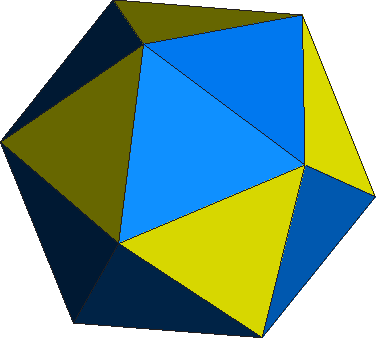
\includegraphics[scale=0.7]{Uniform_polyhedron-43-h01.pdf}
				\end{center}
			\end{enumerate}
		
		For polygons, because $V-E=0$, there are infinte solutions. 
			\subsubsection{More information}
				The Platonic solid have many interesting group properties because their sublime symmetry. (Will be constructed after the test. )
		
	\subsection{Exercise 5.14}
		\subsubsection{Nakahara Exercise 2.14}
			Consider the interval:
				\begin{equation*}
				\begin{aligned}
					(-\varepsilon,\varepsilon)\subset \mathbb{R}
				\end{aligned}
				\end{equation*}
			
			Look at its image:
				\begin{equation*}
				\begin{aligned}
					f((-\varepsilon,\varepsilon))=[0,\varepsilon^2)
				\end{aligned}
				\end{equation*}
			
			Which is not open in $\mathbb{R}$, so the definition "$f$ maps an open set in $X$ to an open set in $Y$" do not work for continuous. 
		
		\subsubsection{Nakahara Exercise 2.17}
			In $\mathbb{R}^2$, the complement of $(0,1)$ is $\mathbb{R}^2\setminus (0,1)$, it is not a open set in usual topology of $\mathbb{R}^2$, so it is niether open or close. Which mean the openness and closeness depend on $X$. 
		
		\subsubsection{Nakahara Problem 2.1}
			Showing this using language	is pale. Using a video is the most stirring way, see: \url{https://www.youtube.com/watch?v=G1yyfPShgqw} and \url{https://www.youtube.com/watch?v=RBWwlfcftYM}. This is a proof without any words. 
		
		\subsubsection{Nakahara Problem 2.2}
			The  complement of the first set is:
				\begin{equation*}
				\begin{aligned}
					C_{\mathbb{R}}(X)=(1,+\infty)\cup (\frac{1}{2},1)\cup \cdots \cup(\frac{1}{n},\frac{1}{n-1})\cup \cdots \cup(-\infty,0]
				\end{aligned}
				\end{equation*}
			
			Is not open in $\mathbb{R}$, so it is not closed. 
			
			The complement of the second set is:
				\begin{equation*}
				\begin{aligned}
					C_{\mathbb{R}}(Y)=(1,+\infty)\cup (\frac{1}{2},1)\cup \cdots \cup(\frac{1}{n},\frac{1}{n-1})\cup \cdots \cup(-\infty,0)
				\end{aligned}
				\end{equation*}
			
			Is open in $\mathbb{R}$, so it is closed, hence compact. 
		
		\subsubsection{Nakahara Problem 2.3}
			Using the surgery, we may cut the first loop with two dots identified, then put one inside another loop, and put them together to get the second picture. So they are homomorphic. In $\mathbb{R}^4$, we can seperate them directly. \footnote{I don't know how to imagine it in $\mathbb{R}^4$...}
		
		\subsubsection{Nakahara Problem 2.4}
			Just Exercise 5.13.  
	
	\subsection{Exercise 5.15}
		According to the definition, we just need to construct two maps from $\mathbb{R}^n\setminus \{0\}$ to $S^{n-1}$. We set:
			\begin{equation*}
			\begin{aligned}
				&f:\mathbb{R}^n\setminus \{0\}\rightarrow S^{n-1},f(v)=\frac{v}{|v|}\\
				&g:S^{n-1}\to \mathbb{R}^n\setminus \{0\}: g(v)=v
			\end{aligned}
			\end{equation*}
		
		We can see that:
			\begin{equation*}
			\begin{aligned}
				f\circ g=\operatorname{id}_y\sim \operatorname{id}_y
			\end{aligned}
			\end{equation*}
		
		To show $g\circ f\sim \operatorname{id}_x$, we should construct a series of functions:
			\begin{equation*}
			\begin{array}{c}
				F(t,x)=tx+\frac{x}{|x|}(1-t)\\
				\begin{cases}
					F(0,x)=\frac{x}{|x|}=g\circ f(x)\\
					F(1,x)=x=\operatorname{id}_x
				\end{cases}
				\Rightarrow g\circ f\sim \operatorname{id}_x
			\end{array}
			\end{equation*}
		
		So $\mathbb{R}^n\setminus \{0\}$ is homotopic to $S^{n-1}$. 
	
	\subsection{Exercise 5.16}
		The homotopy class can be constructed by the function:
			\begin{equation*}
			\begin{aligned}
				f:X\to Y,f(\theta)=\me^{n \mi \theta}
			\end{aligned}
			\end{equation*}
		
		It is characterized by the integer $n$. 
	\subsection{Exercise 5.17}
		We should show that $[\alpha]\to P_{\eta}([\alpha])=[\eta^{-1} \circ \alpha \circ \eta]$ is first a homomorphism. Since for $[\alpha],[\beta] \in \pi_{1}\left(X, x_{0}\right),$ we have
			\begin{equation*}
			\begin{aligned}
			P_{\eta}([\alpha] *[\beta]) &=\left[\eta^{-1}\right] *[\alpha] *[\beta] *[\eta] \\
			&=\left[\eta^{-1}\right] *[\alpha] *[\eta] *\left[\eta^{-1}\right] *[\beta] *[\eta] \\
			&=P_{\eta}([\alpha]) * P_{\eta}([\beta])
			\end{aligned}
			\end{equation*}
		
		To show that $P_{\eta}$ is bijective, we introduce the inverse of $P_{\eta} .$ Define a map $P_{\eta}^{-1}: \pi_{1}\left(X, x_{1}\right) \rightarrow \pi_{1}\left(X, x_{0}\right)$ whose action on $\left[\alpha^{\prime}\right]$ is $P_{\eta}^{-1}\left(\left[\alpha^{\prime}\right]\right)=\left[\eta * \alpha * \eta^{-1}\right]$.
		
		Clearly $P^{-1}$ is the inverse of $P_{\eta}$ since
			\begin{equation*}
			\begin{aligned}
				P_{\eta}^{-1} \circ P_{\eta}([\alpha])=P_{\eta}^{-1}\left(\left[\eta^{-1} * \alpha * \eta\right]\right)=\left[\eta * \eta^{-1} * \alpha * \eta * \eta^{-1}\right]=[\alpha]
			\end{aligned}
			\end{equation*}
		
		Thus, $P_{\eta}^{-1} \circ P_{\eta}=\mathrm{id}_{\pi_{1}\left(X, x_{0}\right)} .$ From the symmetry, we have $P_{\eta} \circ P_{\eta}^{-1}=\mathrm{id}_{\pi_{1}\left(X, x_{1}\right)}$.
		So it is bijective. 
	
	\subsection{Exercise 5.18}
		The loop can wind disk with two holes freely, so the group looks like:
			\begin{equation*}
			\begin{aligned}
				\pi_1(D^2/\{x_1,x_2\})=<x,y;\emptyset>
			\end{aligned}
			\end{equation*}
		
		It is a free group with two generators, so it can also be written as $\mathbb{Z}*\mathbb{Z}$, where $*$ is called the free product. 
	
	\subsection{Exercise 5.19}
		We can set the maximal tree of the triangulation as the red line:
			\begin{center}
				
				
				\tikzset{every picture/.style={line width=0.75pt}} %set default line width to 0.75pt        
				
				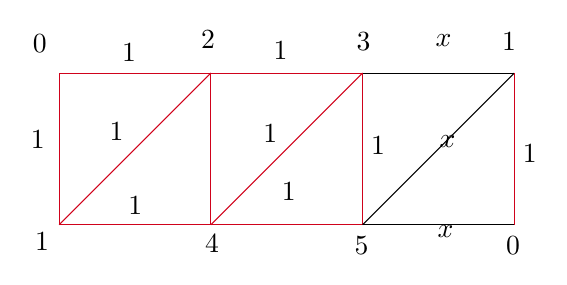
\begin{tikzpicture}[x=0.75pt,y=0.75pt,yscale=-1,xscale=1]
				%uncomment if require: \path (0,300); %set diagram left start at 0, and has height of 300
				
				%Shape: Square [id:dp705475817973492] 
				\draw   (290.08,118) -- (363.17,118) -- (363.17,191.08) -- (290.08,191.08) -- cycle ;
				%Shape: Square [id:dp1564102220918877] 
				\draw  [color={rgb, 255:red, 208; green, 2; blue, 27 }  ,draw opacity=1 ] (143.92,118) -- (217,118) -- (217,191.08) -- (143.92,191.08) -- cycle ;
				%Shape: Square [id:dp9416766880398807] 
				\draw  [color={rgb, 255:red, 208; green, 2; blue, 27 }  ,draw opacity=1 ] (217,118) -- (290.08,118) -- (290.08,191.08) -- (217,191.08) -- cycle ;
				%Straight Lines [id:da5773927617308025] 
				\draw [color={rgb, 255:red, 208; green, 2; blue, 27 }  ,draw opacity=1 ]   (143.92,191.08) -- (217,118) ;
				%Straight Lines [id:da3652823518731222] 
				\draw [color={rgb, 255:red, 208; green, 2; blue, 27 }  ,draw opacity=1 ]   (217,191.08) -- (290.08,118) ;
				%Straight Lines [id:da6868838953176627] 
				\draw    (290.08,191.08) -- (363.17,118) ;
				%Straight Lines [id:da1380904516955439] 
				\draw [color={rgb, 255:red, 208; green, 2; blue, 27 }  ,draw opacity=1 ]   (363.17,118) -- (363.17,191.08) ;
				
				% Text Node
				\draw (130,98.4) node [anchor=north west][inner sep=0.75pt]    {$0$};
				% Text Node
				\draw (131,193.4) node [anchor=north west][inner sep=0.75pt]    {$1$};
				% Text Node
				\draw (211,96.4) node [anchor=north west][inner sep=0.75pt]    {$2$};
				% Text Node
				\draw (286,97.4) node [anchor=north west][inner sep=0.75pt]    {$3$};
				% Text Node
				\draw (356,97.4) node [anchor=north west][inner sep=0.75pt]    {$1$};
				% Text Node
				\draw (213,194.48) node [anchor=north west][inner sep=0.75pt]    {$4$};
				% Text Node
				\draw (285,195.48) node [anchor=north west][inner sep=0.75pt]    {$5$};
				% Text Node
				\draw (358,195.48) node [anchor=north west][inner sep=0.75pt]    {$0$};
				% Text Node
				\draw (129,144.4) node [anchor=north west][inner sep=0.75pt]    {$\mathds{1}$};
				% Text Node
				\draw (173,102.4) node [anchor=north west][inner sep=0.75pt]    {$\mathds{1}$};
				% Text Node
				\draw (246,101.4) node [anchor=north west][inner sep=0.75pt]    {$\mathds{1}$};
				% Text Node
				\draw (167,140.4) node [anchor=north west][inner sep=0.75pt]    {$\mathds{1}$};
				% Text Node
				\draw (176,176.4) node [anchor=north west][inner sep=0.75pt]    {$\mathds{1}$};
				% Text Node
				\draw (241,141.4) node [anchor=north west][inner sep=0.75pt]    {$\mathds{1}$};
				% Text Node
				\draw (250,169.4) node [anchor=north west][inner sep=0.75pt]    {$\mathds{1}$};
				% Text Node
				\draw (293,147.4) node [anchor=north west][inner sep=0.75pt]    {$\mathds{1}$};
				% Text Node
				\draw (324,98) node [anchor=north west][inner sep=0.75pt]   [align=left] {$\displaystyle x$};
				% Text Node
				\draw (366,151.4) node [anchor=north west][inner sep=0.75pt]    {$\mathds{1}$};
				% Text Node
				\draw (326,147) node [anchor=north west][inner sep=0.75pt]   [align=left] {$\displaystyle x$};
				% Text Node
				\draw (325,190) node [anchor=north west][inner sep=0.75pt]   [align=left] {$\displaystyle x$};
				
				
				\end{tikzpicture}
				
			\end{center}
		
		We can see that the fundamental group of Mobius strip is $\mathbb{Z}$, because it has only one free generator. You can also find that the Mobius strip is of the same homotopic type to $S^1$, so $\pi_1(M)=\pi_1(S^1)=\mathbb{Z}$.
	\subsection{Exercise 5.20}
		The maximum tree is a single point because there is only one point on the picture. So:
			\begin{center}
				
				
				\tikzset{every picture/.style={line width=0.75pt}} %set default line width to 0.75pt        
				
				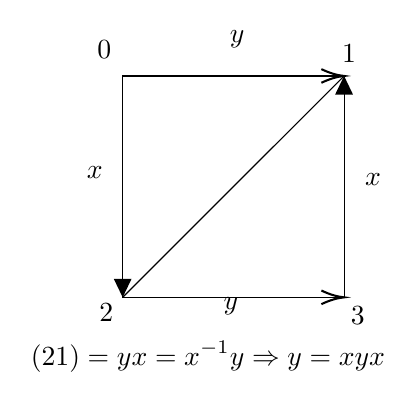
\begin{tikzpicture}[x=0.75pt,y=0.75pt,yscale=-1,xscale=1]
				%uncomment if require: \path (0,300); %set diagram left start at 0, and has height of 300
				
				%Shape: Square [id:dp9816623679140548] 
				\draw   (245.5,83.42) -- (352.17,83.42) -- (352.17,190.08) -- (245.5,190.08) -- cycle ;
				%Straight Lines [id:da6072078445583516] 
				\draw    (245.5,190.08) -- (352.17,83.42) ;
				%Straight Lines [id:da21265045675712602] 
				\draw    (245.5,83.42) -- (350.17,83.42) ;
				\draw [shift={(352.17,83.42)}, rotate = 180] [color={rgb, 255:red, 0; green, 0; blue, 0 }  ][line width=0.75]    (10.93,-3.29) .. controls (6.95,-1.4) and (3.31,-0.3) .. (0,0) .. controls (3.31,0.3) and (6.95,1.4) .. (10.93,3.29)   ;
				%Straight Lines [id:da659849530365877] 
				\draw    (245.5,190.08) -- (350.17,190.08) ;
				\draw [shift={(352.17,190.08)}, rotate = 180] [color={rgb, 255:red, 0; green, 0; blue, 0 }  ][line width=0.75]    (10.93,-3.29) .. controls (6.95,-1.4) and (3.31,-0.3) .. (0,0) .. controls (3.31,0.3) and (6.95,1.4) .. (10.93,3.29)   ;
				%Straight Lines [id:da9909151622213801] 
				\draw    (245.5,83.42) -- (245.5,187.08) ;
				\draw [shift={(245.5,190.08)}, rotate = 270] [fill={rgb, 255:red, 0; green, 0; blue, 0 }  ][line width=0.08]  [draw opacity=0] (8.93,-4.29) -- (0,0) -- (8.93,4.29) -- cycle    ;
				%Straight Lines [id:da7827270735913856] 
				\draw    (352.17,190.08) -- (352.17,86.42) ;
				\draw [shift={(352.17,83.42)}, rotate = 450] [fill={rgb, 255:red, 0; green, 0; blue, 0 }  ][line width=0.08]  [draw opacity=0] (8.93,-4.29) -- (0,0) -- (8.93,4.29) -- cycle    ;
				
				% Text Node
				\draw (232,65) node [anchor=north west][inner sep=0.75pt]   [align=left] {$\displaystyle 0$};
				% Text Node
				\draw (350,67) node [anchor=north west][inner sep=0.75pt]   [align=left] {$\displaystyle 1$};
				% Text Node
				\draw (233,192) node [anchor=north west][inner sep=0.75pt]   [align=left] {$\displaystyle 2$};
				% Text Node
				\draw (354.17,193.08) node [anchor=north west][inner sep=0.75pt]   [align=left] {$\displaystyle 3$};
				% Text Node
				\draw (227,126) node [anchor=north west][inner sep=0.75pt]   [align=left] {$\displaystyle x$};
				% Text Node
				\draw (361,129) node [anchor=north west][inner sep=0.75pt]   [align=left] {$\displaystyle x$};
				% Text Node
				\draw (295.83,60.42) node [anchor=north west][inner sep=0.75pt]   [align=left] {$\displaystyle y$};
				% Text Node
				\draw (292.83,189.08) node [anchor=north west][inner sep=0.75pt]   [align=left] {$\displaystyle y$};
				% Text Node
				\draw (200,210) node [anchor=north west][inner sep=0.75pt]   [align=left] {$\displaystyle ( 21) =yx =x^{-1} y\Rightarrow y=xyx$};
				
				
				\end{tikzpicture}
				
			\end{center}
		
		So the group is just:
			\begin{equation*}
			\begin{aligned}
				\pi_1(K)=<x,y;xyxy^{-1}>
			\end{aligned}
			\end{equation*}
			
	\subsection{Exercise 5.21}
		We can view a point $x=(x_1,x_2,x_3,x_4)$ on $S^3$ as a pair of complex number $(z_1,z_2)$, where $z_1=x_1+\mi x_2,z_2=x_3+\mi x_4$, and they should satisify
			\begin{equation*}
			\begin{aligned}
				|z_1|^2+|z_2|^2=1
			\end{aligned}
			\end{equation*}  
		
		Consider the complex number $\frac{z_1}{z_2}$, when $z_2=0$, it is mapped to the Riemann sphere $\mathbb{C}\cup \{\infty\}$. So this map $ f(x)=\frac{z_1}{z_2} $ is a map $S^3\to S^2$. This is the element $1$. It "winds" the $S^2$ one time, so if you want to construct another element, just map it to $\left(\frac{z_1}{z_2} \right)^n$, it is the element $n$ in $\pi_3(S^2)=\mathbb{Z}$. So the element $0$ is just $f(x)=1$, map all number to a point. 
		
	\subsection{Exercise 5.22}
		This proof is from Hatcher,2002. 
		
		We may assume the polynomial is of the form $p(z)=z^{n}+a_{1} z^{n-1}+\cdots+a_{n}$
		If $p(z)$ has no roots in $\mathbb{C}$, then for each real number $r \geq 0$ the formula
			\begin{equation*}
			\begin{aligned}
			f_{r}(s)=\frac{p\left(r \me^{2 \pi i s}\right) / p(r)}{\left|p\left(r \me^{2 \pi i s}\right) / p(r)\right|}
			\end{aligned}
			\end{equation*}
		
		defines a loop in the unit circle $S^{1} \subset \mathbb{C}$ based at $1 .$ As $r$ varies, $f_{r}$ is a homotopy of loops based at $1 .$ since $f_{0}$ is the trivial loop, we deduce that the class $\left[f_{r}\right] \in \pi_{1}\left(S^{1}\right)$ is zero for all $r$. Now fix a large value of $r,$ bigger than $\left|a_{1}\right|+\cdots+\left|a_{n}\right|$ and bigger than $1 .$ Then for $|z|=r$ we have
			\begin{equation*}
			\begin{aligned}
			\left|z^{n}\right|=r^{n}=r \cdot r^{n-1}>\left(\left|a_{1}\right|+\cdots+\left|a_{n}\right|\right)\left|z^{n-1}\right| \geq\left|a_{1} z^{n-1}+\cdots+a_{n}\right|
			\end{aligned}
			\end{equation*}
		
		From the inequality $\left|z^{n}\right|>\left|a_{1} z^{n-1}+\cdots+a_{n}\right|$ it follows that the polynomial $p_{t}(z)=$ $z^{n}+t\left(a_{1} z^{n-1}+\cdots+a_{n}\right)$ has no roots on the circle $|z|=r$ when $0 \leq t \leq 1 .$ Replacing
		$p$ by $p_{t}$ in the formula for $f_{r}$ above and letting $t$ go from 1 to $0,$ we obtain a homotopy from the loop $f_{r}$ to the loop $\omega_{n}(s)=e^{2 \pi i n s} .$ By Theorem $1.7, \omega_{n}$ represents
		$n$ times a generator of the infinite cyclic group $\pi_{1}\left(S^{1}\right) .$ since we have shown that $\left[\omega_{n}\right]=\left[f_{r}\right]=0,$ we conclude that $n=0 .$ Thus the only polynomials without roots
		in $\mathbb{C}$ are constants.
	\subsection{Exercise 5.23}
		This proof is also from Hatcher,2002. 
		
		 If the conclusion is false for $f: S^{2} \rightarrow \mathbb{R}^{2},$ we can define a map $g: S^{2} \rightarrow S^{1}$ by $g(x)=\frac{f(x)-f(-x)}{|f(x)-f(-x)|}.$ Define a loop $\eta$ circling the equator of $S^{2} \subset \mathbb{R}^{3}$ by $\eta(s)=(\cos 2 \pi s, \sin 2 \pi s, 0),$ and let $h: I \rightarrow S^{1}$ be the composed loop $g \eta$
		since $g(-x)=-g(x),$ we have the relation $h(s+\frac{1}{2})=-h(s)$ for all $s$ in the interval $[0,\frac{1}{2}] .$ As the calculation of $\pi_{1}\left(S^{1}\right),$ the loop $h$ can be lifted to a path $\tilde{h}: I \rightarrow \mathbb{R} .$ The equation $h(s+\frac{1}{2})=-h(s)$ implies that $\tilde{h}(s+\frac{1}{2})=\tilde{h}(s)+\frac{q}{2}$ for
		some odd integer $q$ that might conceivably depend on $s \in[0,\frac{1}{2}] .$ But in fact $q$ is independent of $s$ since by solving the equation $\tilde{h}(s+\frac{1}{2})=\tilde{h}(s)+\frac{q}{2}$ for $q$ we see that $q$ depends continuously on $s \in[0,\frac{1}{2}],$ so $q$ must be a constant since it is constrained to integer values. In particular, we have $\tilde{h}(1)=\tilde{h}(\frac{1}{2})+\frac{q}{2}=\tilde{h}(0)+q .$ This means that $h$ represents $q$ times a generator of $\pi_{1}\left(S^{1}\right) .$ since $q$ is odd, we conclude that $h$ is not nullhomotopic(homotopic
		to a constant map). But $h$ was the composition $g \eta: I \rightarrow S^{2} \rightarrow S^{1},$ and $\eta$ is obviously nullhomotopic in $S^{2},$ so $g \eta$ is nullhomotopic in $S^{1}$ by composing a nullhomotopy of $\eta$ with $g$. Thus we have arrived at a contradiction.
	\subsection{Exercise 5.24}
		\subsubsection{}
			Consider the deformation:
				\begin{equation*}
				\begin{aligned}
					F_t(L)=[R(\theta)t+(1-t)]\me^{i\phi(\theta)}
				\end{aligned}
				\end{equation*}
			
			When $t=1$, $F_1=R(\theta)\me ^{\mi\phi(\theta)}$, when $t=0$, $F_0=\me^{i\phi(\theta)}$, it is a continuous deformation from $R(\theta)$ to 1.
		
		\subsubsection{}
			Because we have $ \phi(2\pi)=2\pi \nu $, construct
				\begin{equation*}
				\begin{aligned}
					F_t=\me^{\mi \phi(\theta)t+(1-t)\nu\theta}
				\end{aligned}
				\end{equation*}
			
			is OK. 
			
	\subsection{Exercise 5.25}
		什么时候学过这玩意了
		
	\subsection{Exercise 5.26}
		\subsubsection{Nakahara Exercise 4.2}
			Like example 4.1, we set:$f:S^n\to D^{n+1}:f(\omega(\theta))=\omega(\theta)$, where $\omega(\theta)$ is the function about the angle of the sphere, has nothing to do with the radius. And $g:D^{n+1}\to S^n:g(r\omega(\theta)) =\omega(\theta)$. We have $g\circ f=\operatorname{id}_x$. To see $f\circ g\sim \operatorname{id}_y$, we construct  
				\begin{equation*}
				\begin{aligned}
					H(r\omega(\theta),t)=[1+(r-1)(1-t)]\omega(\theta)
				\end{aligned}
				\end{equation*}
			
			So it is a deformation retract. 
		
		\subsubsection{Nakahara Exercise 4.5}
			Juset Exercise 5.19.
		
		\subsubsection{Nakahara Problem 4.2}
			This proof follows Hatcher, 2002. 
			
			Suppose on the contrary that $f(x) \neq x$ for all $x \in D^{2}$. Then we can define a map $r: D^{2} \rightarrow S^{1}$ by letting $r(x)$ be the point of $S^{1}$ where the ray in $\mathbb{R}^{2}$ starting at $f(x)$ and passing through $x$ leaves $D^{2}$. Continuity of $r$ is clear since small perturbations of $ x $ produce small perturbations of $f(x)$…, hence
			also small perturbations of the ray through these two points.
			The crucial property of $ r $ , besides continuity, is that $r(x)=x$ if $x \in S^{1} .$ Thus $r$ is a retraction of $D^{2}$ onto $S^{1}$. We will show that no such retraction can exist.
			
			Let $f_{0}$ be any loop in $S^{1} .$ In $D^{2}$ there is a homotopy of $f_{0}$ to a constant loop, for example the linear homotopy $f_{t}(s)=(1-t) f_{0}(s)+t x_{0}$ where $x_{0}$ is the basepoint of $f_{0} .$ Since the retraction $r$ is the identity on $S^{1}$, the composition $r f_{t}$ is then a homotopy in $S^{1}$ from $r f_{0}=f_{0}$ to the constant loop at $x_{0} .$ But this contradicts the fact that $\pi_{1}\left(S^{1}\right)$ is nonzero. 
			
		\subsubsection{Nakahara Problem 4.3}
			Done in Exercise 5.21. 
	
	\subsection{Exercise 5.27}
		We know that $C_p$ is the group generated freely by the generators, so it obviously forms a group.  For a sequence(not exact!):
			\begin{equation*}
			\begin{aligned}
				0\xlongrightarrow[]{i}C_n(K)\xlongrightarrow[]{\pa_n}C_{n-1}(K)\xlongrightarrow[]{\pa_{n-1}}\cdots\xlongrightarrow[]{\pa_2}C_1(K)\xlongrightarrow[]{\pa_1}C_0(K)\xlongrightarrow[]{\pa_0}0
			\end{aligned}
			\end{equation*}	
			
		Note that $Z_r(K)=\operatorname{ker}\pa_r$ and $B_r(K)=\operatorname{im}\pa_{r+1}$, according to Exercise 2.19, they both form a subgroup of the cycle group. 
		
		To prove $B_r(K)\subset Z_r(K)$, we shall first prove: The composite map $\partial_{r} \circ \partial_{r+1}: C_{r+1}(K) \rightarrow C_{r-1}(K)$ is a zero map; that is, $\partial_{r}\left(\partial_{r+1} c\right)=0$ for any $c \in C_{r+1}(K)$.
		
		Since $\partial_{r}$ is a linear operator on $C_{r}(K),$ it is sufficient to prove the identity $\partial_{r} \circ \partial_{r+1}=0$ for the generators of $C_{r+1}(K) .$ If $r=0, \partial_{0} \circ \partial_{1}=0$ since $\partial_{0}$ is a
		zero operator. Let us assume $r>0 .$ Take $\sigma=\left(p_{0} \ldots p_{r} p_{r+1}\right) \in C_{r+1}(K) $. We find
			\begin{equation*}
			\begin{aligned}
				\partial_{r}\left(\partial_{r+1} \sigma\right)=& \partial_{r} \sum_{i=0}^{r+1}(-1)^{i}\left(p_{0} \ldots \hat{p}_{i} \ldots p_{r+1}\right) \\
				=& \sum_{i=0}^{r+1}(-1)^{i} \partial_{r}\left(p_{0} \ldots \hat{p}_{i} \ldots p_{r+1}\right) \\
				=& \sum_{i=0}^{r+1}(-1)^{i}\left(\sum_{j=0}^{i-1}(-1)^{j}\left(p_{0} \ldots \hat{p}_{j} \ldots \hat{p}_{i} \ldots p_{r+1}\right)\right.\left.+\sum_{j=i+1}^{r+1}(-1)^{j-1}\left(p_{0} \ldots \hat{p}_{i} \ldots \hat{p}_{j} \ldots p_{r+1}\right)\right) \\
				=& \sum_{j<i}(-1)^{i+j}\left(p_{0} \ldots \hat{p}_{j} \ldots \hat{p}_{i} \ldots p_{r+1}\right) -\sum_{j>i}(-1)^{i+j}\left(p_{0} \ldots \hat{p}_{i} \ldots \hat{p}_{j} \ldots p_{r+1}\right)=0
			\end{aligned}
			\end{equation*}
			
		Any element $c$ of $B_{r}(K)$ is written as $c=\partial_{r+1} d$ for some $d \in C_{r+1}(K) .$ Then we find $\partial_{r} c=\partial_{r}\left(\partial_{r+1} d\right)=0,$ that is, $c \in Z_{r}(K) .$ This implies $Z_{r}(K) \supset B_{r}(K)$.
		
		For cocyle and cochain, this statement also applies. (这实际上意味着我不会证)
			
			
	\subsection{Exercise 5.28}
		The triangulation of a torus can be drawn  as follows:
			\begin{center}
				
				
				\tikzset{every picture/.style={line width=0.75pt}} %set default line width to 0.75pt        
				
				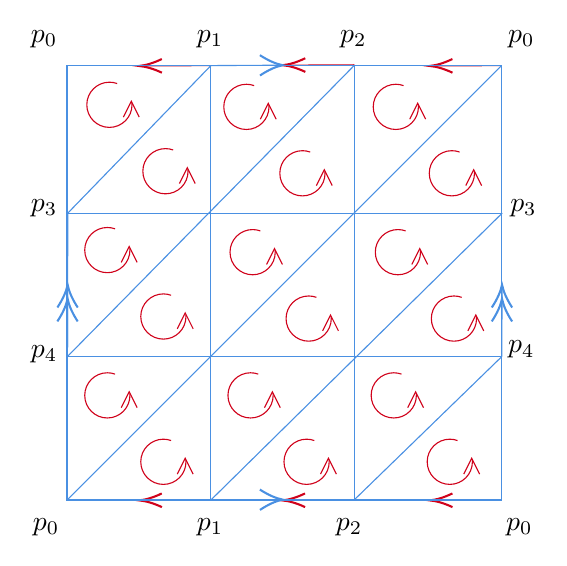
\begin{tikzpicture}[x=0.75pt,y=0.75pt,yscale=-1,xscale=1]
				%uncomment if require: \path (0,300); %set diagram left start at 0, and has height of 300
				
				%Straight Lines [id:da12975974955141434] 
				\draw [color={rgb, 255:red, 208; green, 2; blue, 27 }  ,draw opacity=1 ]   (277.44,252.48) -- (310,252.3) ;
				\draw [shift={(275.44,252.49)}, rotate = 359.68] [color={rgb, 255:red, 208; green, 2; blue, 27 }  ,draw opacity=1 ][line width=0.75]    (10.93,-3.29) .. controls (6.95,-1.4) and (3.31,-0.3) .. (0,0) .. controls (3.31,0.3) and (6.95,1.4) .. (10.93,3.29)   ;
				%Straight Lines [id:da006603073591493813] 
				\draw [color={rgb, 255:red, 208; green, 2; blue, 27 }  ,draw opacity=1 ]   (346.44,252.48) -- (379,252.3) ;
				\draw [shift={(344.44,252.49)}, rotate = 359.68] [color={rgb, 255:red, 208; green, 2; blue, 27 }  ,draw opacity=1 ][line width=0.75]    (10.93,-3.29) .. controls (6.95,-1.4) and (3.31,-0.3) .. (0,0) .. controls (3.31,0.3) and (6.95,1.4) .. (10.93,3.29)   ;
				%Straight Lines [id:da5821723186258224] 
				\draw [color={rgb, 255:red, 208; green, 2; blue, 27 }  ,draw opacity=1 ]   (417.44,252.48) -- (450,252.3) ;
				\draw [shift={(415.44,252.49)}, rotate = 359.68] [color={rgb, 255:red, 208; green, 2; blue, 27 }  ,draw opacity=1 ][line width=0.75]    (10.93,-3.29) .. controls (6.95,-1.4) and (3.31,-0.3) .. (0,0) .. controls (3.31,0.3) and (6.95,1.4) .. (10.93,3.29)   ;
				%Straight Lines [id:da34605847478698804] 
				\draw [color={rgb, 255:red, 208; green, 2; blue, 27 }  ,draw opacity=1 ]   (277.44,43.18) -- (310,43) ;
				\draw [shift={(275.44,43.19)}, rotate = 359.68] [color={rgb, 255:red, 208; green, 2; blue, 27 }  ,draw opacity=1 ][line width=0.75]    (10.93,-3.29) .. controls (6.95,-1.4) and (3.31,-0.3) .. (0,0) .. controls (3.31,0.3) and (6.95,1.4) .. (10.93,3.29)   ;
				%Straight Lines [id:da7255408226920809] 
				\draw [color={rgb, 255:red, 208; green, 2; blue, 27 }  ,draw opacity=1 ]   (346.56,42.8) -- (379.12,42.62) ;
				\draw [shift={(344.56,42.81)}, rotate = 359.68] [color={rgb, 255:red, 208; green, 2; blue, 27 }  ,draw opacity=1 ][line width=0.75]    (10.93,-3.29) .. controls (6.95,-1.4) and (3.31,-0.3) .. (0,0) .. controls (3.31,0.3) and (6.95,1.4) .. (10.93,3.29)   ;
				%Straight Lines [id:da13194970289269314] 
				\draw [color={rgb, 255:red, 208; green, 2; blue, 27 }  ,draw opacity=1 ]   (417.44,43.18) -- (450,43) ;
				\draw [shift={(415.44,43.19)}, rotate = 359.68] [color={rgb, 255:red, 208; green, 2; blue, 27 }  ,draw opacity=1 ][line width=0.75]    (10.93,-3.29) .. controls (6.95,-1.4) and (3.31,-0.3) .. (0,0) .. controls (3.31,0.3) and (6.95,1.4) .. (10.93,3.29)   ;
				%Shape: Square [id:dp7573066185024687] 
				\draw  [color={rgb, 255:red, 74; green, 144; blue, 226 }  ,draw opacity=1 ] (240.7,43) -- (450,43) -- (450,252.3) -- (240.7,252.3) -- cycle ;
				%Straight Lines [id:da05829604853668369] 
				\draw [color={rgb, 255:red, 74; green, 144; blue, 226 }  ,draw opacity=1 ]   (450,43) -- (240.7,252.3) ;
				%Straight Lines [id:da08093732584473712] 
				\draw [color={rgb, 255:red, 74; green, 144; blue, 226 }  ,draw opacity=1 ]   (240.88,183.18) -- (450.18,183.18) ;
				%Straight Lines [id:da4585759146119469] 
				\draw [color={rgb, 255:red, 74; green, 144; blue, 226 }  ,draw opacity=1 ]   (241.07,114.07) -- (450.37,114.07) ;
				%Straight Lines [id:da44619514297861396] 
				\draw [color={rgb, 255:red, 74; green, 144; blue, 226 }  ,draw opacity=1 ]   (379,43) -- (379,252.3) ;
				%Straight Lines [id:da24832222667796033] 
				\draw [color={rgb, 255:red, 74; green, 144; blue, 226 }  ,draw opacity=1 ]   (310,43) -- (310,252.3) ;
				%Straight Lines [id:da6337764235553986] 
				\draw [color={rgb, 255:red, 74; green, 144; blue, 226 }  ,draw opacity=1 ]   (310,43) -- (241.07,114.07) ;
				%Straight Lines [id:da16426972425751474] 
				\draw [color={rgb, 255:red, 74; green, 144; blue, 226 }  ,draw opacity=1 ]   (450.18,183.18) -- (379,252.3) ;
				%Straight Lines [id:da9763634764671117] 
				\draw [color={rgb, 255:red, 74; green, 144; blue, 226 }  ,draw opacity=1 ]   (379,43) -- (240.88,183.18) ;
				%Straight Lines [id:da9794952493994652] 
				\draw [color={rgb, 255:red, 74; green, 144; blue, 226 }  ,draw opacity=1 ]   (450.37,114.07) -- (310,252.3) ;
				%Shape: Arc [id:dp7209520288082216] 
				\draw  [draw opacity=0] (298.97,93.09) .. controls (298.99,93.36) and (299,93.62) .. (299,93.89) .. controls (299,99.91) and (294.12,104.78) .. (288.11,104.78) .. controls (282.09,104.78) and (277.22,99.91) .. (277.22,93.89) .. controls (277.22,87.88) and (282.09,83) .. (288.11,83) .. controls (289.42,83) and (290.67,83.23) .. (291.83,83.65) -- (288.11,93.89) -- cycle ; \draw  [color={rgb, 255:red, 208; green, 2; blue, 27 }  ,draw opacity=1 ] (298.97,93.09) .. controls (298.99,93.36) and (299,93.62) .. (299,93.89) .. controls (299,99.91) and (294.12,104.78) .. (288.11,104.78) .. controls (282.09,104.78) and (277.22,99.91) .. (277.22,93.89) .. controls (277.22,87.88) and (282.09,83) .. (288.11,83) .. controls (289.42,83) and (290.67,83.23) .. (291.83,83.65) ;
				\draw  [color={rgb, 255:red, 208; green, 2; blue, 27 }  ,draw opacity=1 ] (294.82,99.82) -- (298.64,92.18) -- (302.46,99.82) ;
				%Shape: Arc [id:dp7872933029921446] 
				\draw  [draw opacity=0] (271.97,61.09) .. controls (271.99,61.36) and (272,61.62) .. (272,61.89) .. controls (272,67.91) and (267.12,72.78) .. (261.11,72.78) .. controls (255.09,72.78) and (250.22,67.91) .. (250.22,61.89) .. controls (250.22,55.88) and (255.09,51) .. (261.11,51) .. controls (262.42,51) and (263.67,51.23) .. (264.83,51.65) -- (261.11,61.89) -- cycle ; \draw  [color={rgb, 255:red, 208; green, 2; blue, 27 }  ,draw opacity=1 ] (271.97,61.09) .. controls (271.99,61.36) and (272,61.62) .. (272,61.89) .. controls (272,67.91) and (267.12,72.78) .. (261.11,72.78) .. controls (255.09,72.78) and (250.22,67.91) .. (250.22,61.89) .. controls (250.22,55.88) and (255.09,51) .. (261.11,51) .. controls (262.42,51) and (263.67,51.23) .. (264.83,51.65) ;
				\draw  [color={rgb, 255:red, 208; green, 2; blue, 27 }  ,draw opacity=1 ] (267.82,67.82) -- (271.64,60.18) -- (275.46,67.82) ;
				%Shape: Arc [id:dp4034585496476397] 
				\draw  [draw opacity=0] (364.97,94.09) .. controls (364.99,94.36) and (365,94.62) .. (365,94.89) .. controls (365,100.91) and (360.12,105.78) .. (354.11,105.78) .. controls (348.09,105.78) and (343.22,100.91) .. (343.22,94.89) .. controls (343.22,88.88) and (348.09,84) .. (354.11,84) .. controls (355.42,84) and (356.67,84.23) .. (357.83,84.65) -- (354.11,94.89) -- cycle ; \draw  [color={rgb, 255:red, 208; green, 2; blue, 27 }  ,draw opacity=1 ] (364.97,94.09) .. controls (364.99,94.36) and (365,94.62) .. (365,94.89) .. controls (365,100.91) and (360.12,105.78) .. (354.11,105.78) .. controls (348.09,105.78) and (343.22,100.91) .. (343.22,94.89) .. controls (343.22,88.88) and (348.09,84) .. (354.11,84) .. controls (355.42,84) and (356.67,84.23) .. (357.83,84.65) ;
				\draw  [color={rgb, 255:red, 208; green, 2; blue, 27 }  ,draw opacity=1 ] (360.82,100.82) -- (364.64,93.18) -- (368.46,100.82) ;
				%Shape: Arc [id:dp06954968444098608] 
				\draw  [draw opacity=0] (337.97,62.09) .. controls (337.99,62.36) and (338,62.62) .. (338,62.89) .. controls (338,68.91) and (333.12,73.78) .. (327.11,73.78) .. controls (321.09,73.78) and (316.22,68.91) .. (316.22,62.89) .. controls (316.22,56.88) and (321.09,52) .. (327.11,52) .. controls (328.42,52) and (329.67,52.23) .. (330.83,52.65) -- (327.11,62.89) -- cycle ; \draw  [color={rgb, 255:red, 208; green, 2; blue, 27 }  ,draw opacity=1 ] (337.97,62.09) .. controls (337.99,62.36) and (338,62.62) .. (338,62.89) .. controls (338,68.91) and (333.12,73.78) .. (327.11,73.78) .. controls (321.09,73.78) and (316.22,68.91) .. (316.22,62.89) .. controls (316.22,56.88) and (321.09,52) .. (327.11,52) .. controls (328.42,52) and (329.67,52.23) .. (330.83,52.65) ;
				\draw  [color={rgb, 255:red, 208; green, 2; blue, 27 }  ,draw opacity=1 ] (333.82,68.82) -- (337.64,61.18) -- (341.46,68.82) ;
				%Shape: Arc [id:dp24987707325253505] 
				\draw  [draw opacity=0] (436.97,94.09) .. controls (436.99,94.36) and (437,94.62) .. (437,94.89) .. controls (437,100.91) and (432.12,105.78) .. (426.11,105.78) .. controls (420.09,105.78) and (415.22,100.91) .. (415.22,94.89) .. controls (415.22,88.88) and (420.09,84) .. (426.11,84) .. controls (427.42,84) and (428.67,84.23) .. (429.83,84.65) -- (426.11,94.89) -- cycle ; \draw  [color={rgb, 255:red, 208; green, 2; blue, 27 }  ,draw opacity=1 ] (436.97,94.09) .. controls (436.99,94.36) and (437,94.62) .. (437,94.89) .. controls (437,100.91) and (432.12,105.78) .. (426.11,105.78) .. controls (420.09,105.78) and (415.22,100.91) .. (415.22,94.89) .. controls (415.22,88.88) and (420.09,84) .. (426.11,84) .. controls (427.42,84) and (428.67,84.23) .. (429.83,84.65) ;
				\draw  [color={rgb, 255:red, 208; green, 2; blue, 27 }  ,draw opacity=1 ] (432.82,100.82) -- (436.64,93.18) -- (440.46,100.82) ;
				%Shape: Arc [id:dp8163527719768139] 
				\draw  [draw opacity=0] (409.97,62.09) .. controls (409.99,62.36) and (410,62.62) .. (410,62.89) .. controls (410,68.91) and (405.12,73.78) .. (399.11,73.78) .. controls (393.09,73.78) and (388.22,68.91) .. (388.22,62.89) .. controls (388.22,56.88) and (393.09,52) .. (399.11,52) .. controls (400.42,52) and (401.67,52.23) .. (402.83,52.65) -- (399.11,62.89) -- cycle ; \draw  [color={rgb, 255:red, 208; green, 2; blue, 27 }  ,draw opacity=1 ] (409.97,62.09) .. controls (409.99,62.36) and (410,62.62) .. (410,62.89) .. controls (410,68.91) and (405.12,73.78) .. (399.11,73.78) .. controls (393.09,73.78) and (388.22,68.91) .. (388.22,62.89) .. controls (388.22,56.88) and (393.09,52) .. (399.11,52) .. controls (400.42,52) and (401.67,52.23) .. (402.83,52.65) ;
				\draw  [color={rgb, 255:red, 208; green, 2; blue, 27 }  ,draw opacity=1 ] (405.82,68.82) -- (409.64,61.18) -- (413.46,68.82) ;
				%Shape: Arc [id:dp7466598820276591] 
				\draw  [draw opacity=0] (297.97,163.09) .. controls (297.99,163.36) and (298,163.62) .. (298,163.89) .. controls (298,169.91) and (293.12,174.78) .. (287.11,174.78) .. controls (281.09,174.78) and (276.22,169.91) .. (276.22,163.89) .. controls (276.22,157.88) and (281.09,153) .. (287.11,153) .. controls (288.42,153) and (289.67,153.23) .. (290.83,153.65) -- (287.11,163.89) -- cycle ; \draw  [color={rgb, 255:red, 208; green, 2; blue, 27 }  ,draw opacity=1 ] (297.97,163.09) .. controls (297.99,163.36) and (298,163.62) .. (298,163.89) .. controls (298,169.91) and (293.12,174.78) .. (287.11,174.78) .. controls (281.09,174.78) and (276.22,169.91) .. (276.22,163.89) .. controls (276.22,157.88) and (281.09,153) .. (287.11,153) .. controls (288.42,153) and (289.67,153.23) .. (290.83,153.65) ;
				\draw  [color={rgb, 255:red, 208; green, 2; blue, 27 }  ,draw opacity=1 ] (293.82,169.82) -- (297.64,162.18) -- (301.46,169.82) ;
				%Shape: Arc [id:dp37924697889634673] 
				\draw  [draw opacity=0] (270.97,131.09) .. controls (270.99,131.36) and (271,131.62) .. (271,131.89) .. controls (271,137.91) and (266.12,142.78) .. (260.11,142.78) .. controls (254.09,142.78) and (249.22,137.91) .. (249.22,131.89) .. controls (249.22,125.88) and (254.09,121) .. (260.11,121) .. controls (261.42,121) and (262.67,121.23) .. (263.83,121.65) -- (260.11,131.89) -- cycle ; \draw  [color={rgb, 255:red, 208; green, 2; blue, 27 }  ,draw opacity=1 ] (270.97,131.09) .. controls (270.99,131.36) and (271,131.62) .. (271,131.89) .. controls (271,137.91) and (266.12,142.78) .. (260.11,142.78) .. controls (254.09,142.78) and (249.22,137.91) .. (249.22,131.89) .. controls (249.22,125.88) and (254.09,121) .. (260.11,121) .. controls (261.42,121) and (262.67,121.23) .. (263.83,121.65) ;
				\draw  [color={rgb, 255:red, 208; green, 2; blue, 27 }  ,draw opacity=1 ] (266.82,137.82) -- (270.64,130.18) -- (274.46,137.82) ;
				%Shape: Arc [id:dp31837390169970803] 
				\draw  [draw opacity=0] (367.97,164.09) .. controls (367.99,164.36) and (368,164.62) .. (368,164.89) .. controls (368,170.91) and (363.12,175.78) .. (357.11,175.78) .. controls (351.09,175.78) and (346.22,170.91) .. (346.22,164.89) .. controls (346.22,158.88) and (351.09,154) .. (357.11,154) .. controls (358.42,154) and (359.67,154.23) .. (360.83,154.65) -- (357.11,164.89) -- cycle ; \draw  [color={rgb, 255:red, 208; green, 2; blue, 27 }  ,draw opacity=1 ] (367.97,164.09) .. controls (367.99,164.36) and (368,164.62) .. (368,164.89) .. controls (368,170.91) and (363.12,175.78) .. (357.11,175.78) .. controls (351.09,175.78) and (346.22,170.91) .. (346.22,164.89) .. controls (346.22,158.88) and (351.09,154) .. (357.11,154) .. controls (358.42,154) and (359.67,154.23) .. (360.83,154.65) ;
				\draw  [color={rgb, 255:red, 208; green, 2; blue, 27 }  ,draw opacity=1 ] (363.82,170.82) -- (367.64,163.18) -- (371.46,170.82) ;
				%Shape: Arc [id:dp2028152805193415] 
				\draw  [draw opacity=0] (340.97,132.09) .. controls (340.99,132.36) and (341,132.62) .. (341,132.89) .. controls (341,138.91) and (336.12,143.78) .. (330.11,143.78) .. controls (324.09,143.78) and (319.22,138.91) .. (319.22,132.89) .. controls (319.22,126.88) and (324.09,122) .. (330.11,122) .. controls (331.42,122) and (332.67,122.23) .. (333.83,122.65) -- (330.11,132.89) -- cycle ; \draw  [color={rgb, 255:red, 208; green, 2; blue, 27 }  ,draw opacity=1 ] (340.97,132.09) .. controls (340.99,132.36) and (341,132.62) .. (341,132.89) .. controls (341,138.91) and (336.12,143.78) .. (330.11,143.78) .. controls (324.09,143.78) and (319.22,138.91) .. (319.22,132.89) .. controls (319.22,126.88) and (324.09,122) .. (330.11,122) .. controls (331.42,122) and (332.67,122.23) .. (333.83,122.65) ;
				\draw  [color={rgb, 255:red, 208; green, 2; blue, 27 }  ,draw opacity=1 ] (336.82,138.82) -- (340.64,131.18) -- (344.46,138.82) ;
				%Shape: Arc [id:dp9055638850542023] 
				\draw  [draw opacity=0] (437.97,164.09) .. controls (437.99,164.36) and (438,164.62) .. (438,164.89) .. controls (438,170.91) and (433.12,175.78) .. (427.11,175.78) .. controls (421.09,175.78) and (416.22,170.91) .. (416.22,164.89) .. controls (416.22,158.88) and (421.09,154) .. (427.11,154) .. controls (428.42,154) and (429.67,154.23) .. (430.83,154.65) -- (427.11,164.89) -- cycle ; \draw  [color={rgb, 255:red, 208; green, 2; blue, 27 }  ,draw opacity=1 ] (437.97,164.09) .. controls (437.99,164.36) and (438,164.62) .. (438,164.89) .. controls (438,170.91) and (433.12,175.78) .. (427.11,175.78) .. controls (421.09,175.78) and (416.22,170.91) .. (416.22,164.89) .. controls (416.22,158.88) and (421.09,154) .. (427.11,154) .. controls (428.42,154) and (429.67,154.23) .. (430.83,154.65) ;
				\draw  [color={rgb, 255:red, 208; green, 2; blue, 27 }  ,draw opacity=1 ] (433.82,170.82) -- (437.64,163.18) -- (441.46,170.82) ;
				%Shape: Arc [id:dp5372233498165411] 
				\draw  [draw opacity=0] (410.97,132.09) .. controls (410.99,132.36) and (411,132.62) .. (411,132.89) .. controls (411,138.91) and (406.12,143.78) .. (400.11,143.78) .. controls (394.09,143.78) and (389.22,138.91) .. (389.22,132.89) .. controls (389.22,126.88) and (394.09,122) .. (400.11,122) .. controls (401.42,122) and (402.67,122.23) .. (403.83,122.65) -- (400.11,132.89) -- cycle ; \draw  [color={rgb, 255:red, 208; green, 2; blue, 27 }  ,draw opacity=1 ] (410.97,132.09) .. controls (410.99,132.36) and (411,132.62) .. (411,132.89) .. controls (411,138.91) and (406.12,143.78) .. (400.11,143.78) .. controls (394.09,143.78) and (389.22,138.91) .. (389.22,132.89) .. controls (389.22,126.88) and (394.09,122) .. (400.11,122) .. controls (401.42,122) and (402.67,122.23) .. (403.83,122.65) ;
				\draw  [color={rgb, 255:red, 208; green, 2; blue, 27 }  ,draw opacity=1 ] (406.82,138.82) -- (410.64,131.18) -- (414.46,138.82) ;
				%Shape: Arc [id:dp006601356142885928] 
				\draw  [draw opacity=0] (297.97,233.09) .. controls (297.99,233.36) and (298,233.62) .. (298,233.89) .. controls (298,239.91) and (293.12,244.78) .. (287.11,244.78) .. controls (281.09,244.78) and (276.22,239.91) .. (276.22,233.89) .. controls (276.22,227.88) and (281.09,223) .. (287.11,223) .. controls (288.42,223) and (289.67,223.23) .. (290.83,223.65) -- (287.11,233.89) -- cycle ; \draw  [color={rgb, 255:red, 208; green, 2; blue, 27 }  ,draw opacity=1 ] (297.97,233.09) .. controls (297.99,233.36) and (298,233.62) .. (298,233.89) .. controls (298,239.91) and (293.12,244.78) .. (287.11,244.78) .. controls (281.09,244.78) and (276.22,239.91) .. (276.22,233.89) .. controls (276.22,227.88) and (281.09,223) .. (287.11,223) .. controls (288.42,223) and (289.67,223.23) .. (290.83,223.65) ;
				\draw  [color={rgb, 255:red, 208; green, 2; blue, 27 }  ,draw opacity=1 ] (293.82,239.82) -- (297.64,232.18) -- (301.46,239.82) ;
				%Shape: Arc [id:dp7375656683954145] 
				\draw  [draw opacity=0] (270.97,201.09) .. controls (270.99,201.36) and (271,201.62) .. (271,201.89) .. controls (271,207.91) and (266.12,212.78) .. (260.11,212.78) .. controls (254.09,212.78) and (249.22,207.91) .. (249.22,201.89) .. controls (249.22,195.88) and (254.09,191) .. (260.11,191) .. controls (261.42,191) and (262.67,191.23) .. (263.83,191.65) -- (260.11,201.89) -- cycle ; \draw  [color={rgb, 255:red, 208; green, 2; blue, 27 }  ,draw opacity=1 ] (270.97,201.09) .. controls (270.99,201.36) and (271,201.62) .. (271,201.89) .. controls (271,207.91) and (266.12,212.78) .. (260.11,212.78) .. controls (254.09,212.78) and (249.22,207.91) .. (249.22,201.89) .. controls (249.22,195.88) and (254.09,191) .. (260.11,191) .. controls (261.42,191) and (262.67,191.23) .. (263.83,191.65) ;
				\draw  [color={rgb, 255:red, 208; green, 2; blue, 27 }  ,draw opacity=1 ] (266.82,207.82) -- (270.64,200.18) -- (274.46,207.82) ;
				%Shape: Arc [id:dp0094891616211501] 
				\draw  [draw opacity=0] (366.97,233.09) .. controls (366.99,233.36) and (367,233.62) .. (367,233.89) .. controls (367,239.91) and (362.12,244.78) .. (356.11,244.78) .. controls (350.09,244.78) and (345.22,239.91) .. (345.22,233.89) .. controls (345.22,227.88) and (350.09,223) .. (356.11,223) .. controls (357.42,223) and (358.67,223.23) .. (359.83,223.65) -- (356.11,233.89) -- cycle ; \draw  [color={rgb, 255:red, 208; green, 2; blue, 27 }  ,draw opacity=1 ] (366.97,233.09) .. controls (366.99,233.36) and (367,233.62) .. (367,233.89) .. controls (367,239.91) and (362.12,244.78) .. (356.11,244.78) .. controls (350.09,244.78) and (345.22,239.91) .. (345.22,233.89) .. controls (345.22,227.88) and (350.09,223) .. (356.11,223) .. controls (357.42,223) and (358.67,223.23) .. (359.83,223.65) ;
				\draw  [color={rgb, 255:red, 208; green, 2; blue, 27 }  ,draw opacity=1 ] (362.82,239.82) -- (366.64,232.18) -- (370.46,239.82) ;
				%Shape: Arc [id:dp49948035281886616] 
				\draw  [draw opacity=0] (339.97,201.09) .. controls (339.99,201.36) and (340,201.62) .. (340,201.89) .. controls (340,207.91) and (335.12,212.78) .. (329.11,212.78) .. controls (323.09,212.78) and (318.22,207.91) .. (318.22,201.89) .. controls (318.22,195.88) and (323.09,191) .. (329.11,191) .. controls (330.42,191) and (331.67,191.23) .. (332.83,191.65) -- (329.11,201.89) -- cycle ; \draw  [color={rgb, 255:red, 208; green, 2; blue, 27 }  ,draw opacity=1 ] (339.97,201.09) .. controls (339.99,201.36) and (340,201.62) .. (340,201.89) .. controls (340,207.91) and (335.12,212.78) .. (329.11,212.78) .. controls (323.09,212.78) and (318.22,207.91) .. (318.22,201.89) .. controls (318.22,195.88) and (323.09,191) .. (329.11,191) .. controls (330.42,191) and (331.67,191.23) .. (332.83,191.65) ;
				\draw  [color={rgb, 255:red, 208; green, 2; blue, 27 }  ,draw opacity=1 ] (335.82,207.82) -- (339.64,200.18) -- (343.46,207.82) ;
				%Shape: Arc [id:dp6649550170930679] 
				\draw  [draw opacity=0] (435.97,233.09) .. controls (435.99,233.36) and (436,233.62) .. (436,233.89) .. controls (436,239.91) and (431.12,244.78) .. (425.11,244.78) .. controls (419.09,244.78) and (414.22,239.91) .. (414.22,233.89) .. controls (414.22,227.88) and (419.09,223) .. (425.11,223) .. controls (426.42,223) and (427.67,223.23) .. (428.83,223.65) -- (425.11,233.89) -- cycle ; \draw  [color={rgb, 255:red, 208; green, 2; blue, 27 }  ,draw opacity=1 ] (435.97,233.09) .. controls (435.99,233.36) and (436,233.62) .. (436,233.89) .. controls (436,239.91) and (431.12,244.78) .. (425.11,244.78) .. controls (419.09,244.78) and (414.22,239.91) .. (414.22,233.89) .. controls (414.22,227.88) and (419.09,223) .. (425.11,223) .. controls (426.42,223) and (427.67,223.23) .. (428.83,223.65) ;
				\draw  [color={rgb, 255:red, 208; green, 2; blue, 27 }  ,draw opacity=1 ] (431.82,239.82) -- (435.64,232.18) -- (439.46,239.82) ;
				%Shape: Arc [id:dp6998736358293304] 
				\draw  [draw opacity=0] (408.97,201.09) .. controls (408.99,201.36) and (409,201.62) .. (409,201.89) .. controls (409,207.91) and (404.12,212.78) .. (398.11,212.78) .. controls (392.09,212.78) and (387.22,207.91) .. (387.22,201.89) .. controls (387.22,195.88) and (392.09,191) .. (398.11,191) .. controls (399.42,191) and (400.67,191.23) .. (401.83,191.65) -- (398.11,201.89) -- cycle ; \draw  [color={rgb, 255:red, 208; green, 2; blue, 27 }  ,draw opacity=1 ] (408.97,201.09) .. controls (408.99,201.36) and (409,201.62) .. (409,201.89) .. controls (409,207.91) and (404.12,212.78) .. (398.11,212.78) .. controls (392.09,212.78) and (387.22,207.91) .. (387.22,201.89) .. controls (387.22,195.88) and (392.09,191) .. (398.11,191) .. controls (399.42,191) and (400.67,191.23) .. (401.83,191.65) ;
				\draw  [color={rgb, 255:red, 208; green, 2; blue, 27 }  ,draw opacity=1 ] (404.82,207.82) -- (408.64,200.18) -- (412.46,207.82) ;
				%Straight Lines [id:da07404908636974483] 
				\draw [color={rgb, 255:red, 74; green, 144; blue, 226 }  ,draw opacity=1 ]   (240.88,183.18) -- (241.07,114.07) ;
				%Straight Lines [id:da011596147240479304] 
				\draw [color={rgb, 255:red, 74; green, 144; blue, 226 }  ,draw opacity=1 ]   (240.88,183.18) -- (240.98,148.62) ;
				\draw [shift={(240.98,148.62)}, rotate = 450.15] [color={rgb, 255:red, 74; green, 144; blue, 226 }  ,draw opacity=1 ][line width=0.75]    (17.64,-4.9) .. controls (13.66,-2.3) and (10.02,-0.67) .. (6.71,0) .. controls (10.02,0.67) and (13.66,2.3) .. (17.64,4.9)(10.93,-4.9) .. controls (6.95,-2.3) and (3.31,-0.67) .. (0,0) .. controls (3.31,0.67) and (6.95,2.3) .. (10.93,4.9)   ;
				%Straight Lines [id:da3786708302167596] 
				\draw [color={rgb, 255:red, 74; green, 144; blue, 226 }  ,draw opacity=1 ]   (450.18,183.18) -- (450.28,148.62) ;
				\draw [shift={(450.28,148.62)}, rotate = 450.15] [color={rgb, 255:red, 74; green, 144; blue, 226 }  ,draw opacity=1 ][line width=0.75]    (17.64,-4.9) .. controls (13.66,-2.3) and (10.02,-0.67) .. (6.71,0) .. controls (10.02,0.67) and (13.66,2.3) .. (17.64,4.9)(10.93,-4.9) .. controls (6.95,-2.3) and (3.31,-0.67) .. (0,0) .. controls (3.31,0.67) and (6.95,2.3) .. (10.93,4.9)   ;
				%Straight Lines [id:da4067936371918056] 
				\draw [color={rgb, 255:red, 74; green, 144; blue, 226 }  ,draw opacity=1 ]   (310,43) -- (342.56,42.82) ;
				\draw [shift={(344.56,42.81)}, rotate = 539.6800000000001] [color={rgb, 255:red, 74; green, 144; blue, 226 }  ,draw opacity=1 ][line width=0.75]    (10.93,-4.9) .. controls (6.95,-2.3) and (3.31,-0.67) .. (0,0) .. controls (3.31,0.67) and (6.95,2.3) .. (10.93,4.9)   ;
				%Straight Lines [id:da36882024470646546] 
				\draw [color={rgb, 255:red, 74; green, 144; blue, 226 }  ,draw opacity=1 ]   (310,252.3) -- (342.56,252.12) ;
				\draw [shift={(344.56,252.11)}, rotate = 539.6800000000001] [color={rgb, 255:red, 74; green, 144; blue, 226 }  ,draw opacity=1 ][line width=0.75]    (10.93,-4.9) .. controls (6.95,-2.3) and (3.31,-0.67) .. (0,0) .. controls (3.31,0.67) and (6.95,2.3) .. (10.93,4.9)   ;
				
				% Text Node
				\draw (222,25) node [anchor=north west][inner sep=0.75pt]    {$p_{0}$};
				% Text Node
				\draw (452,25) node [anchor=north west][inner sep=0.75pt]    {$p_{0}$};
				% Text Node
				\draw (223,260) node [anchor=north west][inner sep=0.75pt]    {$p_{0}$};
				% Text Node
				\draw (451,260) node [anchor=north west][inner sep=0.75pt]    {$p_{0}$};
				% Text Node
				\draw (302,25) node [anchor=north west][inner sep=0.75pt]    {$p_{1}$};
				% Text Node
				\draw (302,260) node [anchor=north west][inner sep=0.75pt]    {$p_{1}$};
				% Text Node
				\draw (371,25) node [anchor=north west][inner sep=0.75pt]    {$p_{2}$};
				% Text Node
				\draw (369,260) node [anchor=north west][inner sep=0.75pt]    {$p_{2}$};
				% Text Node
				\draw (453,106.4) node [anchor=north west][inner sep=0.75pt]    {$p_{3}$};
				% Text Node
				\draw (222,106.4) node [anchor=north west][inner sep=0.75pt]    {$p_{3}$};
				% Text Node
				\draw (452,174.4) node [anchor=north west][inner sep=0.75pt]    {$p_{4}$};
				% Text Node
				\draw (222,176.4) node [anchor=north west][inner sep=0.75pt]    {$p_{4}$};
				
				
				\end{tikzpicture}
				
			\end{center}
		
		However, some unknown theorem ensure that the ``bad trangulation'' can also help us calculate the right homology group. The ``bad trangulation'' looks like:
			\begin{center}
				
				
				\tikzset{every picture/.style={line width=0.75pt}} %set default line width to 0.75pt        
				
				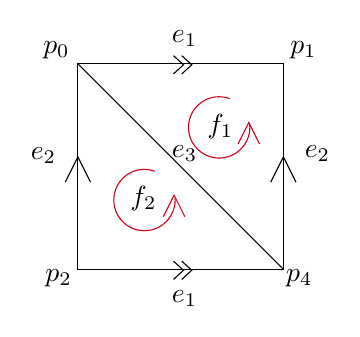
\begin{tikzpicture}[x=0.75pt,y=0.75pt,yscale=-1,xscale=1]
				%uncomment if require: \path (0,300); %set diagram left start at 0, and has height of 300
				
				%Shape: Square [id:dp8232678288359376] 
				\draw   (203.78,102) -- (303,102) -- (303,201.22) -- (203.78,201.22) -- cycle ;
				%Straight Lines [id:da039398508299939405] 
				\draw    (203.78,102) -- (303,201.22) ;
				\draw   (197.83,159.17) -- (203.92,147) -- (210,159.17) ;
				\draw   (296.83,159.17) -- (302.92,147) -- (309,159.17) ;
				\draw   (250,197.22) -- (254.78,201.61) -- (250,206)(254,197.22) -- (258.78,201.61) -- (254,206) ;
				\draw   (250,98.22) -- (254.78,102.61) -- (250,107)(254,98.22) -- (258.78,102.61) -- (254,107) ;
				%Shape: Arc [id:dp6643552858956431] 
				\draw  [draw opacity=0] (286.73,131.69) .. controls (286.75,132.05) and (286.77,132.41) .. (286.77,132.78) .. controls (286.77,140.94) and (280.15,147.55) .. (271.99,147.55) .. controls (263.83,147.55) and (257.22,140.94) .. (257.22,132.78) .. controls (257.22,124.61) and (263.83,118) .. (271.99,118) .. controls (273.77,118) and (275.47,118.31) .. (277.05,118.89) -- (271.99,132.78) -- cycle ; \draw  [color={rgb, 255:red, 208; green, 2; blue, 27 }  ,draw opacity=1 ] (286.73,131.69) .. controls (286.75,132.05) and (286.77,132.41) .. (286.77,132.78) .. controls (286.77,140.94) and (280.15,147.55) .. (271.99,147.55) .. controls (263.83,147.55) and (257.22,140.94) .. (257.22,132.78) .. controls (257.22,124.61) and (263.83,118) .. (271.99,118) .. controls (273.77,118) and (275.47,118.31) .. (277.05,118.89) ;
				\draw  [color={rgb, 255:red, 208; green, 2; blue, 27 }  ,draw opacity=1 ] (281.1,140.81) -- (286.28,130.45) -- (291.46,140.81) ;
				%Shape: Arc [id:dp8253869138952726] 
				\draw  [draw opacity=0] (250.73,166.69) .. controls (250.75,167.05) and (250.77,167.41) .. (250.77,167.78) .. controls (250.77,175.94) and (244.15,182.55) .. (235.99,182.55) .. controls (227.83,182.55) and (221.22,175.94) .. (221.22,167.78) .. controls (221.22,159.61) and (227.83,153) .. (235.99,153) .. controls (237.77,153) and (239.47,153.31) .. (241.05,153.89) -- (235.99,167.78) -- cycle ; \draw  [color={rgb, 255:red, 208; green, 2; blue, 27 }  ,draw opacity=1 ] (250.73,166.69) .. controls (250.75,167.05) and (250.77,167.41) .. (250.77,167.78) .. controls (250.77,175.94) and (244.15,182.55) .. (235.99,182.55) .. controls (227.83,182.55) and (221.22,175.94) .. (221.22,167.78) .. controls (221.22,159.61) and (227.83,153) .. (235.99,153) .. controls (237.77,153) and (239.47,153.31) .. (241.05,153.89) ;
				\draw  [color={rgb, 255:red, 208; green, 2; blue, 27 }  ,draw opacity=1 ] (245.1,175.81) -- (250.28,165.45) -- (255.46,175.81) ;
				
				% Text Node
				\draw (186,90) node [anchor=north west][inner sep=0.75pt]    {$p_{0}$};
				% Text Node
				\draw (305,90) node [anchor=north west][inner sep=0.75pt]    {$p_{1}$};
				% Text Node
				\draw (187,200) node [anchor=north west][inner sep=0.75pt]    {$p_{2}$};
				% Text Node
				\draw (303,200) node [anchor=north west][inner sep=0.75pt]    {$p_{4}$};
				% Text Node
				\draw (248,85) node [anchor=north west][inner sep=0.75pt]    {$e_{1}$};
				% Text Node
				\draw (248,210) node [anchor=north west][inner sep=0.75pt]    {$e_{1}$};
				% Text Node
				\draw (180,141.4) node [anchor=north west][inner sep=0.75pt]    {$e_{2}$};
				% Text Node
				\draw (312,140.4) node [anchor=north west][inner sep=0.75pt]    {$e_{2}$};
				\draw (248,140.4) node [anchor=north west][inner sep=0.75pt]    {$e_{3}$};
				\draw (265,125) node [anchor=north west][inner sep=0.75pt]    {$f_{1}$};
				\draw (228,160) node [anchor=north west][inner sep=0.75pt]    {$f_{2}$};
				\end{tikzpicture}
				
			\end{center}
		
		There are only one vertex on the graph, so with one generator, we have:
			\begin{equation*}
			\begin{aligned}
				C_0(K)=\mathbb{Z}
			\end{aligned}
			\end{equation*}
			
		There are three edges and two faces on the graph, so:
			\begin{equation*}
			\begin{aligned}
				&C_1(K)=\mathbb{Z}\oplus\mathbb{Z}\oplus\mathbb{Z}\\
				&C_2(K)=\mathbb{Z}
			\end{aligned}
			\end{equation*}
			
		Then we calculate its boundary group. The 0-th boundary group is the boundary of 1-chain. 
			\begin{equation*}
			\begin{aligned}
				B_0=\operatorname{im}\pa_1&=\pa_1(b_1e_1+b_2e_2+b_3e_3)\\
				&=b_1(v_2-v_1)+b_2(v_3-v_4)+b_3(v_3-v_1)=\{0\}
			\end{aligned}
			\end{equation*}
			
		Similary:
			\begin{equation*}
			\begin{aligned}
				B_1=\operatorname{im}\pa_2&=\pa_2(a_1f_1+a_2f_2)\\
				&=a_1(e_3-e_1-e_2)+a_2(e_1+e_2-e_3)\\
				&=(a_1-a_2)(e_3-e_1-e_2)=\mathbb{Z}\\
				B_2=\operatorname{im}\pa_3&=\pa_3(0)=\{0\}
			\end{aligned}
			\end{equation*}
			
		So the homology group is
			\begin{equation*}
			\begin{aligned}
				&H_0(K)=C_0/B_0=\mathbb{Z}/\{0\}=\mathbb{Z}\\
				&H_1(K)=C_1/B_1=\mathbb{Z}\oplus\mathbb{Z}\oplus\mathbb{Z}/\mathbb{Z}=\mathbb{Z}\oplus\mathbb{Z}\\
				&H_2(K)=C_2/B_2=\mathbb{Z}/\{0\}=\mathbb{Z}
			\end{aligned}
			\end{equation*}
			
		If we replace the field $\mathbb{Z}$ by $\mathbb{R}$, the homological group is just:
			\begin{equation*}
			\begin{aligned}
				&H_0(K)=\mathbb{R}\\
				&H_1(K)=\mathbb{R}\oplus\mathbb{R}\\
				&H_2(K)=\mathbb{R}
			\end{aligned}
			\end{equation*}	
			
		But I have to mention that, if there are parts that are not freely generated by the generators, like:
			\begin{equation*}
			\begin{aligned}
				H_r(K)=\underbrace{\mathbb{Z}\oplus\mathbb{Z}\oplus\cdots \oplus\mathbb{Z}}_{p}\oplus\underbrace{\mathbb{Z}_{k_1}\oplus\mathbb{Z}_{k_2}\oplus\cdots \oplus\mathbb{Z}_{k_q}}_{q}
			\end{aligned}
			\end{equation*}
			
		Then after replacing $\mathbb{Z}$ by $\mathbb{R}$, there are only freely generated parts left:
			\begin{equation*}
			\begin{aligned}
				H_r(K)=\underbrace{\mathbb{R}\oplus\mathbb{R}\oplus\cdots \oplus\mathbb{R}}_{p}
			\end{aligned}
			\end{equation*}
	
		\subsubsection{More information}
			The minimal legal triangulation of the torus actually looks like:
				\begin{center}
					
					
					\tikzset{every picture/.style={line width=0.75pt}} %set default line width to 0.75pt        
					
					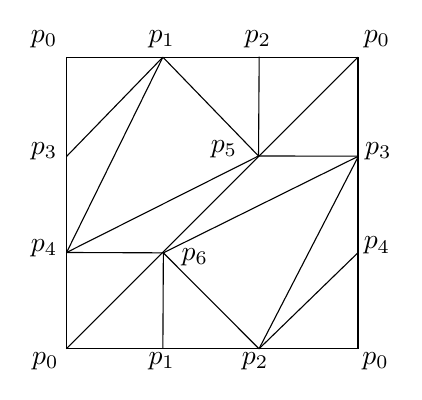
\begin{tikzpicture}[x=0.75pt,y=0.75pt,yscale=-1,xscale=1]
					%uncomment if require: \path (0,300); %set diagram left start at 0, and has height of 300
					
					%Shape: Square [id:dp26031530449036855] 
					\draw  [color={rgb, 255:red, 0; green, 0; blue, 0 }  ,draw opacity=1 ] (245.23,58.94) -- (385.74,58.94) -- (385.74,199.45) -- (245.23,199.45) -- cycle ;
					%Straight Lines [id:da1315164960986126] 
					\draw [color={rgb, 255:red, 0; green, 0; blue, 0 }  ,draw opacity=1 ]   (385.74,58.94) -- (245.23,199.45) ;
					%Straight Lines [id:da1371903492175982] 
					\draw [color={rgb, 255:red, 0; green, 0; blue, 0 }  ,draw opacity=1 ]   (291.75,58.94) -- (245.47,106.65) ;
					%Straight Lines [id:da13366880843022766] 
					\draw    (385.98,106.65) -- (337.83,106.55) ;
					%Straight Lines [id:da47158114999718326] 
					\draw    (337.83,106.55) -- (338.15,58.68) ;
					%Straight Lines [id:da03824285092458013] 
					\draw    (291.98,153.22) -- (291.75,199.45) ;
					%Straight Lines [id:da014370834246032693] 
					\draw    (245.35,153.05) -- (291.98,153.22) ;
					%Straight Lines [id:da15134265707311034] 
					\draw    (385.98,106.65) -- (338.07,199.45) ;
					%Straight Lines [id:da9232417507887569] 
					\draw    (291.98,153.22) -- (338.07,199.45) ;
					%Straight Lines [id:da3572678344158121] 
					\draw    (291.98,153.22) -- (385.98,106.65) ;
					%Straight Lines [id:da03866018388075976] 
					\draw    (385.86,153.05) -- (338.07,199.45) ;
					%Straight Lines [id:da8330930434510696] 
					\draw    (245.35,153.05) -- (337.83,106.55) ;
					%Straight Lines [id:da7816355335120343] 
					\draw    (291.75,58.94) -- (337.83,106.55) ;
					%Straight Lines [id:da43082535747845263] 
					\draw    (245.35,153.05) -- (291.75,58.94) ;
					
					% Text Node
					\draw (226.88,45) node [anchor=north west][inner sep=0.75pt]    {$p_{0}$};
					% Text Node
					\draw (387.28,45) node [anchor=north west][inner sep=0.75pt]    {$p_{0}$};
					% Text Node
					\draw (227.55,200) node [anchor=north west][inner sep=0.75pt]    {$p_{0}$};
					% Text Node
					\draw (386.61,200) node [anchor=north west][inner sep=0.75pt]    {$p_{0}$};
					% Text Node
					\draw (283.58,45) node [anchor=north west][inner sep=0.75pt]    {$p_{1}$};
					% Text Node
					\draw (283.58,200) node [anchor=north west][inner sep=0.75pt]    {$p_{1}$};
					% Text Node
					\draw (329.91,45) node [anchor=north west][inner sep=0.75pt]    {$p_{2}$};
					% Text Node
					\draw (328.56,200) node [anchor=north west][inner sep=0.75pt]    {$p_{2}$};
					% Text Node
					\draw (387.96,98.67) node [anchor=north west][inner sep=0.75pt]    {$p_{3}$};
					% Text Node
					\draw (226.88,98.67) node [anchor=north west][inner sep=0.75pt]    {$p_{3}$};
					% Text Node
					\draw (387.28,144.32) node [anchor=north west][inner sep=0.75pt]    {$p_{4}$};
					% Text Node
					\draw (226.88,145.67) node [anchor=north west][inner sep=0.75pt]    {$p_{4}$};
					% Text Node
					\draw (313.58,98) node [anchor=north west][inner sep=0.75pt]    {$p_{5}$};
					% Text Node
					\draw (299.58,150) node [anchor=north west][inner sep=0.75pt]    {$p_{6}$};
					
					
					\end{tikzpicture}
					
				\end{center}
			
		Although we do not know anything the ``bad triangulation'', do we know anything about the ``good triangualtion''? 
		
	\subsection{Exercise 5.29}
		\subsubsection{Homology group for Klein bottle}
			The trangulation looks like:
				\begin{center}
					
					
					\tikzset{every picture/.style={line width=0.75pt}} %set default line width to 0.75pt        
					
					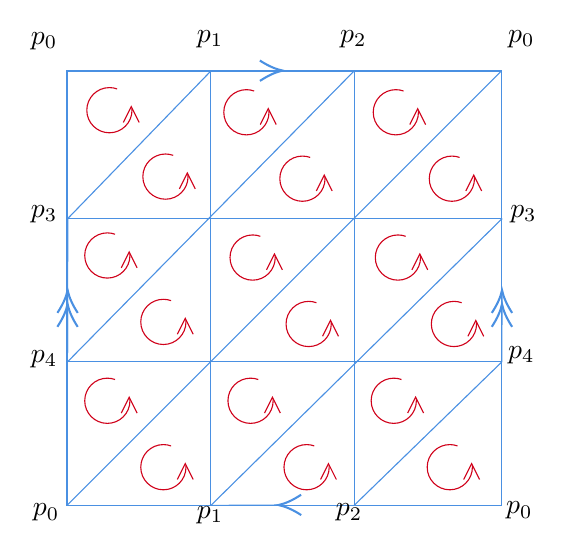
\begin{tikzpicture}[x=0.75pt,y=0.75pt,yscale=-1,xscale=1]
					%uncomment if require: \path (0,300); %set diagram left start at 0, and has height of 300
					
					%Shape: Square [id:dp21535563470205232] 
					\draw  [color={rgb, 255:red, 74; green, 144; blue, 226 }  ,draw opacity=1 ] (260.7,45) -- (470,45) -- (470,254.3) -- (260.7,254.3) -- cycle ;
					%Straight Lines [id:da8898161205453528] 
					\draw [color={rgb, 255:red, 74; green, 144; blue, 226 }  ,draw opacity=1 ]   (470,45) -- (260.7,254.3) ;
					%Straight Lines [id:da6756383234746597] 
					\draw [color={rgb, 255:red, 74; green, 144; blue, 226 }  ,draw opacity=1 ]   (260.88,185.18) -- (470.18,185.18) ;
					%Straight Lines [id:da4228450581650146] 
					\draw [color={rgb, 255:red, 74; green, 144; blue, 226 }  ,draw opacity=1 ]   (261.07,116.07) -- (470.37,116.07) ;
					%Straight Lines [id:da7912200401996248] 
					\draw [color={rgb, 255:red, 74; green, 144; blue, 226 }  ,draw opacity=1 ]   (399,45) -- (399,254.3) ;
					%Straight Lines [id:da046807360056424274] 
					\draw [color={rgb, 255:red, 74; green, 144; blue, 226 }  ,draw opacity=1 ]   (330,45) -- (330,254.3) ;
					%Straight Lines [id:da5089423595086445] 
					\draw [color={rgb, 255:red, 74; green, 144; blue, 226 }  ,draw opacity=1 ]   (330,45) -- (261.07,116.07) ;
					%Straight Lines [id:da8142677195812147] 
					\draw [color={rgb, 255:red, 74; green, 144; blue, 226 }  ,draw opacity=1 ]   (470.18,185.18) -- (399,254.3) ;
					%Straight Lines [id:da7218686701376091] 
					\draw [color={rgb, 255:red, 74; green, 144; blue, 226 }  ,draw opacity=1 ]   (399,45) -- (260.88,185.18) ;
					%Straight Lines [id:da19705056906361096] 
					\draw [color={rgb, 255:red, 74; green, 144; blue, 226 }  ,draw opacity=1 ]   (470.37,116.07) -- (330,254.3) ;
					%Shape: Arc [id:dp6523687526941044] 
					\draw  [draw opacity=0] (318.97,95.09) .. controls (318.99,95.36) and (319,95.62) .. (319,95.89) .. controls (319,101.91) and (314.12,106.78) .. (308.11,106.78) .. controls (302.09,106.78) and (297.22,101.91) .. (297.22,95.89) .. controls (297.22,89.88) and (302.09,85) .. (308.11,85) .. controls (309.42,85) and (310.67,85.23) .. (311.83,85.65) -- (308.11,95.89) -- cycle ; \draw  [color={rgb, 255:red, 208; green, 2; blue, 27 }  ,draw opacity=1 ] (318.97,95.09) .. controls (318.99,95.36) and (319,95.62) .. (319,95.89) .. controls (319,101.91) and (314.12,106.78) .. (308.11,106.78) .. controls (302.09,106.78) and (297.22,101.91) .. (297.22,95.89) .. controls (297.22,89.88) and (302.09,85) .. (308.11,85) .. controls (309.42,85) and (310.67,85.23) .. (311.83,85.65) ;
					\draw  [color={rgb, 255:red, 208; green, 2; blue, 27 }  ,draw opacity=1 ] (314.82,101.82) -- (318.64,94.18) -- (322.46,101.82) ;
					%Shape: Arc [id:dp9464464448266365] 
					\draw  [draw opacity=0] (291.97,63.09) .. controls (291.99,63.36) and (292,63.62) .. (292,63.89) .. controls (292,69.91) and (287.12,74.78) .. (281.11,74.78) .. controls (275.09,74.78) and (270.22,69.91) .. (270.22,63.89) .. controls (270.22,57.88) and (275.09,53) .. (281.11,53) .. controls (282.42,53) and (283.67,53.23) .. (284.83,53.65) -- (281.11,63.89) -- cycle ; \draw  [color={rgb, 255:red, 208; green, 2; blue, 27 }  ,draw opacity=1 ] (291.97,63.09) .. controls (291.99,63.36) and (292,63.62) .. (292,63.89) .. controls (292,69.91) and (287.12,74.78) .. (281.11,74.78) .. controls (275.09,74.78) and (270.22,69.91) .. (270.22,63.89) .. controls (270.22,57.88) and (275.09,53) .. (281.11,53) .. controls (282.42,53) and (283.67,53.23) .. (284.83,53.65) ;
					\draw  [color={rgb, 255:red, 208; green, 2; blue, 27 }  ,draw opacity=1 ] (287.82,69.82) -- (291.64,62.18) -- (295.46,69.82) ;
					%Shape: Arc [id:dp4769158871774303] 
					\draw  [draw opacity=0] (384.97,96.09) .. controls (384.99,96.36) and (385,96.62) .. (385,96.89) .. controls (385,102.91) and (380.12,107.78) .. (374.11,107.78) .. controls (368.09,107.78) and (363.22,102.91) .. (363.22,96.89) .. controls (363.22,90.88) and (368.09,86) .. (374.11,86) .. controls (375.42,86) and (376.67,86.23) .. (377.83,86.65) -- (374.11,96.89) -- cycle ; \draw  [color={rgb, 255:red, 208; green, 2; blue, 27 }  ,draw opacity=1 ] (384.97,96.09) .. controls (384.99,96.36) and (385,96.62) .. (385,96.89) .. controls (385,102.91) and (380.12,107.78) .. (374.11,107.78) .. controls (368.09,107.78) and (363.22,102.91) .. (363.22,96.89) .. controls (363.22,90.88) and (368.09,86) .. (374.11,86) .. controls (375.42,86) and (376.67,86.23) .. (377.83,86.65) ;
					\draw  [color={rgb, 255:red, 208; green, 2; blue, 27 }  ,draw opacity=1 ] (380.82,102.82) -- (384.64,95.18) -- (388.46,102.82) ;
					%Shape: Arc [id:dp6805905944385238] 
					\draw  [draw opacity=0] (357.97,64.09) .. controls (357.99,64.36) and (358,64.62) .. (358,64.89) .. controls (358,70.91) and (353.12,75.78) .. (347.11,75.78) .. controls (341.09,75.78) and (336.22,70.91) .. (336.22,64.89) .. controls (336.22,58.88) and (341.09,54) .. (347.11,54) .. controls (348.42,54) and (349.67,54.23) .. (350.83,54.65) -- (347.11,64.89) -- cycle ; \draw  [color={rgb, 255:red, 208; green, 2; blue, 27 }  ,draw opacity=1 ] (357.97,64.09) .. controls (357.99,64.36) and (358,64.62) .. (358,64.89) .. controls (358,70.91) and (353.12,75.78) .. (347.11,75.78) .. controls (341.09,75.78) and (336.22,70.91) .. (336.22,64.89) .. controls (336.22,58.88) and (341.09,54) .. (347.11,54) .. controls (348.42,54) and (349.67,54.23) .. (350.83,54.65) ;
					\draw  [color={rgb, 255:red, 208; green, 2; blue, 27 }  ,draw opacity=1 ] (353.82,70.82) -- (357.64,63.18) -- (361.46,70.82) ;
					%Shape: Arc [id:dp5114626325904718] 
					\draw  [draw opacity=0] (456.97,96.09) .. controls (456.99,96.36) and (457,96.62) .. (457,96.89) .. controls (457,102.91) and (452.12,107.78) .. (446.11,107.78) .. controls (440.09,107.78) and (435.22,102.91) .. (435.22,96.89) .. controls (435.22,90.88) and (440.09,86) .. (446.11,86) .. controls (447.42,86) and (448.67,86.23) .. (449.83,86.65) -- (446.11,96.89) -- cycle ; \draw  [color={rgb, 255:red, 208; green, 2; blue, 27 }  ,draw opacity=1 ] (456.97,96.09) .. controls (456.99,96.36) and (457,96.62) .. (457,96.89) .. controls (457,102.91) and (452.12,107.78) .. (446.11,107.78) .. controls (440.09,107.78) and (435.22,102.91) .. (435.22,96.89) .. controls (435.22,90.88) and (440.09,86) .. (446.11,86) .. controls (447.42,86) and (448.67,86.23) .. (449.83,86.65) ;
					\draw  [color={rgb, 255:red, 208; green, 2; blue, 27 }  ,draw opacity=1 ] (452.82,102.82) -- (456.64,95.18) -- (460.46,102.82) ;
					%Shape: Arc [id:dp22381665048159027] 
					\draw  [draw opacity=0] (429.97,64.09) .. controls (429.99,64.36) and (430,64.62) .. (430,64.89) .. controls (430,70.91) and (425.12,75.78) .. (419.11,75.78) .. controls (413.09,75.78) and (408.22,70.91) .. (408.22,64.89) .. controls (408.22,58.88) and (413.09,54) .. (419.11,54) .. controls (420.42,54) and (421.67,54.23) .. (422.83,54.65) -- (419.11,64.89) -- cycle ; \draw  [color={rgb, 255:red, 208; green, 2; blue, 27 }  ,draw opacity=1 ] (429.97,64.09) .. controls (429.99,64.36) and (430,64.62) .. (430,64.89) .. controls (430,70.91) and (425.12,75.78) .. (419.11,75.78) .. controls (413.09,75.78) and (408.22,70.91) .. (408.22,64.89) .. controls (408.22,58.88) and (413.09,54) .. (419.11,54) .. controls (420.42,54) and (421.67,54.23) .. (422.83,54.65) ;
					\draw  [color={rgb, 255:red, 208; green, 2; blue, 27 }  ,draw opacity=1 ] (425.82,70.82) -- (429.64,63.18) -- (433.46,70.82) ;
					%Shape: Arc [id:dp2318176516345194] 
					\draw  [draw opacity=0] (317.97,165.09) .. controls (317.99,165.36) and (318,165.62) .. (318,165.89) .. controls (318,171.91) and (313.12,176.78) .. (307.11,176.78) .. controls (301.09,176.78) and (296.22,171.91) .. (296.22,165.89) .. controls (296.22,159.88) and (301.09,155) .. (307.11,155) .. controls (308.42,155) and (309.67,155.23) .. (310.83,155.65) -- (307.11,165.89) -- cycle ; \draw  [color={rgb, 255:red, 208; green, 2; blue, 27 }  ,draw opacity=1 ] (317.97,165.09) .. controls (317.99,165.36) and (318,165.62) .. (318,165.89) .. controls (318,171.91) and (313.12,176.78) .. (307.11,176.78) .. controls (301.09,176.78) and (296.22,171.91) .. (296.22,165.89) .. controls (296.22,159.88) and (301.09,155) .. (307.11,155) .. controls (308.42,155) and (309.67,155.23) .. (310.83,155.65) ;
					\draw  [color={rgb, 255:red, 208; green, 2; blue, 27 }  ,draw opacity=1 ] (313.82,171.82) -- (317.64,164.18) -- (321.46,171.82) ;
					%Shape: Arc [id:dp9588380040336119] 
					\draw  [draw opacity=0] (290.97,133.09) .. controls (290.99,133.36) and (291,133.62) .. (291,133.89) .. controls (291,139.91) and (286.12,144.78) .. (280.11,144.78) .. controls (274.09,144.78) and (269.22,139.91) .. (269.22,133.89) .. controls (269.22,127.88) and (274.09,123) .. (280.11,123) .. controls (281.42,123) and (282.67,123.23) .. (283.83,123.65) -- (280.11,133.89) -- cycle ; \draw  [color={rgb, 255:red, 208; green, 2; blue, 27 }  ,draw opacity=1 ] (290.97,133.09) .. controls (290.99,133.36) and (291,133.62) .. (291,133.89) .. controls (291,139.91) and (286.12,144.78) .. (280.11,144.78) .. controls (274.09,144.78) and (269.22,139.91) .. (269.22,133.89) .. controls (269.22,127.88) and (274.09,123) .. (280.11,123) .. controls (281.42,123) and (282.67,123.23) .. (283.83,123.65) ;
					\draw  [color={rgb, 255:red, 208; green, 2; blue, 27 }  ,draw opacity=1 ] (286.82,139.82) -- (290.64,132.18) -- (294.46,139.82) ;
					%Shape: Arc [id:dp5898600900301004] 
					\draw  [draw opacity=0] (387.97,166.09) .. controls (387.99,166.36) and (388,166.62) .. (388,166.89) .. controls (388,172.91) and (383.12,177.78) .. (377.11,177.78) .. controls (371.09,177.78) and (366.22,172.91) .. (366.22,166.89) .. controls (366.22,160.88) and (371.09,156) .. (377.11,156) .. controls (378.42,156) and (379.67,156.23) .. (380.83,156.65) -- (377.11,166.89) -- cycle ; \draw  [color={rgb, 255:red, 208; green, 2; blue, 27 }  ,draw opacity=1 ] (387.97,166.09) .. controls (387.99,166.36) and (388,166.62) .. (388,166.89) .. controls (388,172.91) and (383.12,177.78) .. (377.11,177.78) .. controls (371.09,177.78) and (366.22,172.91) .. (366.22,166.89) .. controls (366.22,160.88) and (371.09,156) .. (377.11,156) .. controls (378.42,156) and (379.67,156.23) .. (380.83,156.65) ;
					\draw  [color={rgb, 255:red, 208; green, 2; blue, 27 }  ,draw opacity=1 ] (383.82,172.82) -- (387.64,165.18) -- (391.46,172.82) ;
					%Shape: Arc [id:dp19839890486246214] 
					\draw  [draw opacity=0] (360.97,134.09) .. controls (360.99,134.36) and (361,134.62) .. (361,134.89) .. controls (361,140.91) and (356.12,145.78) .. (350.11,145.78) .. controls (344.09,145.78) and (339.22,140.91) .. (339.22,134.89) .. controls (339.22,128.88) and (344.09,124) .. (350.11,124) .. controls (351.42,124) and (352.67,124.23) .. (353.83,124.65) -- (350.11,134.89) -- cycle ; \draw  [color={rgb, 255:red, 208; green, 2; blue, 27 }  ,draw opacity=1 ] (360.97,134.09) .. controls (360.99,134.36) and (361,134.62) .. (361,134.89) .. controls (361,140.91) and (356.12,145.78) .. (350.11,145.78) .. controls (344.09,145.78) and (339.22,140.91) .. (339.22,134.89) .. controls (339.22,128.88) and (344.09,124) .. (350.11,124) .. controls (351.42,124) and (352.67,124.23) .. (353.83,124.65) ;
					\draw  [color={rgb, 255:red, 208; green, 2; blue, 27 }  ,draw opacity=1 ] (356.82,140.82) -- (360.64,133.18) -- (364.46,140.82) ;
					%Shape: Arc [id:dp6850506585483414] 
					\draw  [draw opacity=0] (457.97,166.09) .. controls (457.99,166.36) and (458,166.62) .. (458,166.89) .. controls (458,172.91) and (453.12,177.78) .. (447.11,177.78) .. controls (441.09,177.78) and (436.22,172.91) .. (436.22,166.89) .. controls (436.22,160.88) and (441.09,156) .. (447.11,156) .. controls (448.42,156) and (449.67,156.23) .. (450.83,156.65) -- (447.11,166.89) -- cycle ; \draw  [color={rgb, 255:red, 208; green, 2; blue, 27 }  ,draw opacity=1 ] (457.97,166.09) .. controls (457.99,166.36) and (458,166.62) .. (458,166.89) .. controls (458,172.91) and (453.12,177.78) .. (447.11,177.78) .. controls (441.09,177.78) and (436.22,172.91) .. (436.22,166.89) .. controls (436.22,160.88) and (441.09,156) .. (447.11,156) .. controls (448.42,156) and (449.67,156.23) .. (450.83,156.65) ;
					\draw  [color={rgb, 255:red, 208; green, 2; blue, 27 }  ,draw opacity=1 ] (453.82,172.82) -- (457.64,165.18) -- (461.46,172.82) ;
					%Shape: Arc [id:dp8212979767661319] 
					\draw  [draw opacity=0] (430.97,134.09) .. controls (430.99,134.36) and (431,134.62) .. (431,134.89) .. controls (431,140.91) and (426.12,145.78) .. (420.11,145.78) .. controls (414.09,145.78) and (409.22,140.91) .. (409.22,134.89) .. controls (409.22,128.88) and (414.09,124) .. (420.11,124) .. controls (421.42,124) and (422.67,124.23) .. (423.83,124.65) -- (420.11,134.89) -- cycle ; \draw  [color={rgb, 255:red, 208; green, 2; blue, 27 }  ,draw opacity=1 ] (430.97,134.09) .. controls (430.99,134.36) and (431,134.62) .. (431,134.89) .. controls (431,140.91) and (426.12,145.78) .. (420.11,145.78) .. controls (414.09,145.78) and (409.22,140.91) .. (409.22,134.89) .. controls (409.22,128.88) and (414.09,124) .. (420.11,124) .. controls (421.42,124) and (422.67,124.23) .. (423.83,124.65) ;
					\draw  [color={rgb, 255:red, 208; green, 2; blue, 27 }  ,draw opacity=1 ] (426.82,140.82) -- (430.64,133.18) -- (434.46,140.82) ;
					%Shape: Arc [id:dp8532155779204406] 
					\draw  [draw opacity=0] (317.97,235.09) .. controls (317.99,235.36) and (318,235.62) .. (318,235.89) .. controls (318,241.91) and (313.12,246.78) .. (307.11,246.78) .. controls (301.09,246.78) and (296.22,241.91) .. (296.22,235.89) .. controls (296.22,229.88) and (301.09,225) .. (307.11,225) .. controls (308.42,225) and (309.67,225.23) .. (310.83,225.65) -- (307.11,235.89) -- cycle ; \draw  [color={rgb, 255:red, 208; green, 2; blue, 27 }  ,draw opacity=1 ] (317.97,235.09) .. controls (317.99,235.36) and (318,235.62) .. (318,235.89) .. controls (318,241.91) and (313.12,246.78) .. (307.11,246.78) .. controls (301.09,246.78) and (296.22,241.91) .. (296.22,235.89) .. controls (296.22,229.88) and (301.09,225) .. (307.11,225) .. controls (308.42,225) and (309.67,225.23) .. (310.83,225.65) ;
					\draw  [color={rgb, 255:red, 208; green, 2; blue, 27 }  ,draw opacity=1 ] (313.82,241.82) -- (317.64,234.18) -- (321.46,241.82) ;
					%Shape: Arc [id:dp3870639434542923] 
					\draw  [draw opacity=0] (290.97,203.09) .. controls (290.99,203.36) and (291,203.62) .. (291,203.89) .. controls (291,209.91) and (286.12,214.78) .. (280.11,214.78) .. controls (274.09,214.78) and (269.22,209.91) .. (269.22,203.89) .. controls (269.22,197.88) and (274.09,193) .. (280.11,193) .. controls (281.42,193) and (282.67,193.23) .. (283.83,193.65) -- (280.11,203.89) -- cycle ; \draw  [color={rgb, 255:red, 208; green, 2; blue, 27 }  ,draw opacity=1 ] (290.97,203.09) .. controls (290.99,203.36) and (291,203.62) .. (291,203.89) .. controls (291,209.91) and (286.12,214.78) .. (280.11,214.78) .. controls (274.09,214.78) and (269.22,209.91) .. (269.22,203.89) .. controls (269.22,197.88) and (274.09,193) .. (280.11,193) .. controls (281.42,193) and (282.67,193.23) .. (283.83,193.65) ;
					\draw  [color={rgb, 255:red, 208; green, 2; blue, 27 }  ,draw opacity=1 ] (286.82,209.82) -- (290.64,202.18) -- (294.46,209.82) ;
					%Shape: Arc [id:dp12955157579037313] 
					\draw  [draw opacity=0] (386.97,235.09) .. controls (386.99,235.36) and (387,235.62) .. (387,235.89) .. controls (387,241.91) and (382.12,246.78) .. (376.11,246.78) .. controls (370.09,246.78) and (365.22,241.91) .. (365.22,235.89) .. controls (365.22,229.88) and (370.09,225) .. (376.11,225) .. controls (377.42,225) and (378.67,225.23) .. (379.83,225.65) -- (376.11,235.89) -- cycle ; \draw  [color={rgb, 255:red, 208; green, 2; blue, 27 }  ,draw opacity=1 ] (386.97,235.09) .. controls (386.99,235.36) and (387,235.62) .. (387,235.89) .. controls (387,241.91) and (382.12,246.78) .. (376.11,246.78) .. controls (370.09,246.78) and (365.22,241.91) .. (365.22,235.89) .. controls (365.22,229.88) and (370.09,225) .. (376.11,225) .. controls (377.42,225) and (378.67,225.23) .. (379.83,225.65) ;
					\draw  [color={rgb, 255:red, 208; green, 2; blue, 27 }  ,draw opacity=1 ] (382.82,241.82) -- (386.64,234.18) -- (390.46,241.82) ;
					%Shape: Arc [id:dp5369557114461473] 
					\draw  [draw opacity=0] (359.97,203.09) .. controls (359.99,203.36) and (360,203.62) .. (360,203.89) .. controls (360,209.91) and (355.12,214.78) .. (349.11,214.78) .. controls (343.09,214.78) and (338.22,209.91) .. (338.22,203.89) .. controls (338.22,197.88) and (343.09,193) .. (349.11,193) .. controls (350.42,193) and (351.67,193.23) .. (352.83,193.65) -- (349.11,203.89) -- cycle ; \draw  [color={rgb, 255:red, 208; green, 2; blue, 27 }  ,draw opacity=1 ] (359.97,203.09) .. controls (359.99,203.36) and (360,203.62) .. (360,203.89) .. controls (360,209.91) and (355.12,214.78) .. (349.11,214.78) .. controls (343.09,214.78) and (338.22,209.91) .. (338.22,203.89) .. controls (338.22,197.88) and (343.09,193) .. (349.11,193) .. controls (350.42,193) and (351.67,193.23) .. (352.83,193.65) ;
					\draw  [color={rgb, 255:red, 208; green, 2; blue, 27 }  ,draw opacity=1 ] (355.82,209.82) -- (359.64,202.18) -- (363.46,209.82) ;
					%Shape: Arc [id:dp3530650231444439] 
					\draw  [draw opacity=0] (455.97,235.09) .. controls (455.99,235.36) and (456,235.62) .. (456,235.89) .. controls (456,241.91) and (451.12,246.78) .. (445.11,246.78) .. controls (439.09,246.78) and (434.22,241.91) .. (434.22,235.89) .. controls (434.22,229.88) and (439.09,225) .. (445.11,225) .. controls (446.42,225) and (447.67,225.23) .. (448.83,225.65) -- (445.11,235.89) -- cycle ; \draw  [color={rgb, 255:red, 208; green, 2; blue, 27 }  ,draw opacity=1 ] (455.97,235.09) .. controls (455.99,235.36) and (456,235.62) .. (456,235.89) .. controls (456,241.91) and (451.12,246.78) .. (445.11,246.78) .. controls (439.09,246.78) and (434.22,241.91) .. (434.22,235.89) .. controls (434.22,229.88) and (439.09,225) .. (445.11,225) .. controls (446.42,225) and (447.67,225.23) .. (448.83,225.65) ;
					\draw  [color={rgb, 255:red, 208; green, 2; blue, 27 }  ,draw opacity=1 ] (451.82,241.82) -- (455.64,234.18) -- (459.46,241.82) ;
					%Shape: Arc [id:dp007196893660470494] 
					\draw  [draw opacity=0] (428.97,203.09) .. controls (428.99,203.36) and (429,203.62) .. (429,203.89) .. controls (429,209.91) and (424.12,214.78) .. (418.11,214.78) .. controls (412.09,214.78) and (407.22,209.91) .. (407.22,203.89) .. controls (407.22,197.88) and (412.09,193) .. (418.11,193) .. controls (419.42,193) and (420.67,193.23) .. (421.83,193.65) -- (418.11,203.89) -- cycle ; \draw  [color={rgb, 255:red, 208; green, 2; blue, 27 }  ,draw opacity=1 ] (428.97,203.09) .. controls (428.99,203.36) and (429,203.62) .. (429,203.89) .. controls (429,209.91) and (424.12,214.78) .. (418.11,214.78) .. controls (412.09,214.78) and (407.22,209.91) .. (407.22,203.89) .. controls (407.22,197.88) and (412.09,193) .. (418.11,193) .. controls (419.42,193) and (420.67,193.23) .. (421.83,193.65) ;
					\draw  [color={rgb, 255:red, 208; green, 2; blue, 27 }  ,draw opacity=1 ] (424.82,209.82) -- (428.64,202.18) -- (432.46,209.82) ;
					%Straight Lines [id:da8008563542641082] 
					\draw [color={rgb, 255:red, 74; green, 144; blue, 226 }  ,draw opacity=1 ]   (260.88,185.18) -- (261.07,116.07) ;
					%Straight Lines [id:da07494449595967745] 
					\draw [color={rgb, 255:red, 74; green, 144; blue, 226 }  ,draw opacity=1 ]   (260.88,185.18) -- (260.98,150.62) ;
					\draw [shift={(260.98,150.62)}, rotate = 450.15] [color={rgb, 255:red, 74; green, 144; blue, 226 }  ,draw opacity=1 ][line width=0.75]    (17.64,-4.9) .. controls (13.66,-2.3) and (10.02,-0.67) .. (6.71,0) .. controls (10.02,0.67) and (13.66,2.3) .. (17.64,4.9)(10.93,-4.9) .. controls (6.95,-2.3) and (3.31,-0.67) .. (0,0) .. controls (3.31,0.67) and (6.95,2.3) .. (10.93,4.9)   ;
					%Straight Lines [id:da34670239958249705] 
					\draw [color={rgb, 255:red, 74; green, 144; blue, 226 }  ,draw opacity=1 ]   (470.18,185.18) -- (470.28,150.62) ;
					\draw [shift={(470.28,150.62)}, rotate = 450.15] [color={rgb, 255:red, 74; green, 144; blue, 226 }  ,draw opacity=1 ][line width=0.75]    (17.64,-4.9) .. controls (13.66,-2.3) and (10.02,-0.67) .. (6.71,0) .. controls (10.02,0.67) and (13.66,2.3) .. (17.64,4.9)(10.93,-4.9) .. controls (6.95,-2.3) and (3.31,-0.67) .. (0,0) .. controls (3.31,0.67) and (6.95,2.3) .. (10.93,4.9)   ;
					%Straight Lines [id:da2670823271486953] 
					\draw [color={rgb, 255:red, 74; green, 144; blue, 226 }  ,draw opacity=1 ]   (330,45) -- (362.56,44.82) ;
					\draw [shift={(364.56,44.81)}, rotate = 539.6800000000001] [color={rgb, 255:red, 74; green, 144; blue, 226 }  ,draw opacity=1 ][line width=0.75]    (10.93,-4.9) .. controls (6.95,-2.3) and (3.31,-0.67) .. (0,0) .. controls (3.31,0.67) and (6.95,2.3) .. (10.93,4.9)   ;
					%Straight Lines [id:da45386637705439237] 
					\draw [color={rgb, 255:red, 74; green, 144; blue, 226 }  ,draw opacity=1 ]   (330,254.3) -- (362.56,254.12) ;
					\draw [shift={(362.56,254.12)}, rotate = 359.68] [color={rgb, 255:red, 74; green, 144; blue, 226 }  ,draw opacity=1 ][line width=0.75]    (10.93,-4.9) .. controls (6.95,-2.3) and (3.31,-0.67) .. (0,0) .. controls (3.31,0.67) and (6.95,2.3) .. (10.93,4.9)   ;
					
					% Text Node
					\draw (242,25.4) node [anchor=north west][inner sep=0.75pt]    {$p_{0}$};
					% Text Node
					\draw (472,24.4) node [anchor=north west][inner sep=0.75pt]    {$p_{0}$};
					% Text Node
					\draw (243,252.4) node [anchor=north west][inner sep=0.75pt]    {$p_{0}$};
					% Text Node
					\draw (471,251.4) node [anchor=north west][inner sep=0.75pt]    {$p_{0}$};
					% Text Node
					\draw (322,24.4) node [anchor=north west][inner sep=0.75pt]    {$p_{1}$};
					% Text Node
					\draw (322,253.4) node [anchor=north west][inner sep=0.75pt]    {$p_{1}$};
					% Text Node
					\draw (391,24.4) node [anchor=north west][inner sep=0.75pt]    {$p_{2}$};
					% Text Node
					\draw (389,252.4) node [anchor=north west][inner sep=0.75pt]    {$p_{2}$};
					% Text Node
					\draw (473,108.4) node [anchor=north west][inner sep=0.75pt]    {$p_{3}$};
					% Text Node
					\draw (242,108.4) node [anchor=north west][inner sep=0.75pt]    {$p_{3}$};
					% Text Node
					\draw (472,176.4) node [anchor=north west][inner sep=0.75pt]    {$p_{4}$};
					% Text Node
					\draw (242,178.4) node [anchor=north west][inner sep=0.75pt]    {$p_{4}$};
					
					
					\end{tikzpicture}
					
				\end{center}
			
		We know that it is connected, so 
			\begin{equation*}
			\begin{aligned}
				H_0(K)=\mathbb{Z}
			\end{aligned}
			\end{equation*}
			
		For $H_1(K)$, we can see the cycle $a=(p_0p_4p_3p_0)\neq(p_0p_1p_2p_0)=b$, so there are two generators. But we can see $(p_0p_4p_3p_0)$ is free, so it generates $\mathbb{Z}$. Consider $2b$: 
			\begin{equation*}
			\begin{aligned}
				2b=2\left((p_0p_1)+(p_1p_2)+(p_2p_0)\right)\sim 0
			\end{aligned}
			\end{equation*}
			
		So $b^2=2b=0$, which means it generates $\mathbb{Z}_2$. So
			\begin{equation*}
			\begin{aligned}
				H_1(K)=\mathbb{Z}\oplus \mathbb{Z}_2
			\end{aligned}
			\end{equation*}
			
		For $H_2(K)$, we can see there aren't any 3-simplex, which means $B_2(K)=0$, so $H_2(K)=Z_2(K)$. For $\xi\in Z_2(K)$, we have:
			\begin{equation*}
			\begin{aligned}
				\xi=m\sum_{i=1}^{I_r}\sigma_{2,i}=mK
			\end{aligned}
			\end{equation*}
			
		We know that the boundary of $K$ is actually 
			\begin{equation*}
			\begin{aligned}
				\pa_2K=2\left((p_0p_1)+(p_1p_2)+(p_2p_0)\right)
			\end{aligned}
			\end{equation*}
			
		So:
			\begin{equation*}
			\begin{aligned}
				\pa_2\xi=2m\left((p_0p_1)+(p_1p_2)+(p_2p_0)\right)=0\Rightarrow m=0
			\end{aligned}
			\end{equation*}
			
		Which means $Z_2(K)$ has no nontrivial 2-cycles. 
			\begin{equation*}
			\begin{aligned}
				H_2(K)=\{0\}
			\end{aligned}
			\end{equation*}
			
		Replace the field by $\mathbb{R}$, we will get:
			\begin{equation*}
			\begin{aligned}
				&H_0(K)=\mathbb{R}\\
				&H_1(K)=\mathbb{R}\\
				&H_2(K)=\{0\}
			\end{aligned}
			\end{equation*}
			
		\subsubsection{Homology group for projective plane}
			The triangulation of $\mathbb{R}P^2$ looks like:
				\begin{center}
					
					
					\tikzset{every picture/.style={line width=0.75pt}} %set default line width to 0.75pt        
					
					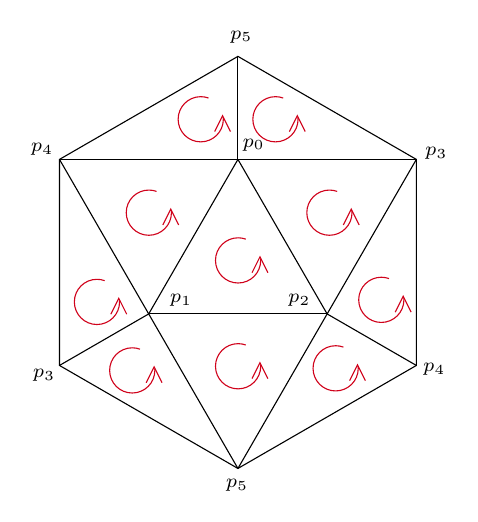
\begin{tikzpicture}[x=0.75pt,y=0.75pt,yscale=-1,xscale=1]
					%uncomment if require: \path (0,300); %set diagram left start at 0, and has height of 300
					
					%Shape: Polygon [id:dp9755917860410769] 
					\draw   (412,91.23) -- (412,190.5) -- (326.03,240.13) -- (240.06,190.5) -- (240.06,91.23) -- (326.03,41.59) -- cycle ;
					%Straight Lines [id:da9552392613333698] 
					\draw    (240.06,91.23) -- (412,91.23) ;
					%Straight Lines [id:da3989135772162429] 
					\draw    (326.03,41.59) -- (326.03,91.23) ;
					%Straight Lines [id:da1257339267353783] 
					\draw    (240.06,91.23) -- (326.03,240.13) ;
					%Straight Lines [id:da277102156580711] 
					\draw    (412,91.23) -- (326.03,240.13) ;
					%Straight Lines [id:da9031792310648437] 
					\draw    (240.06,190.5) -- (283.04,165.68) ;
					%Straight Lines [id:da42496817136161935] 
					\draw    (369.01,165.68) -- (412,190.5) ;
					%Straight Lines [id:da5293245594911715] 
					\draw    (326.03,91.23) -- (369.01,165.68) ;
					%Straight Lines [id:da8735915826867884] 
					\draw    (326.03,91.23) -- (283.04,165.68) ;
					%Straight Lines [id:da9811568857881835] 
					\draw    (283.04,165.68) -- (369.01,165.68) ;
					%Shape: Arc [id:dp3113187481047085] 
					\draw  [draw opacity=0] (336.97,190.09) .. controls (336.99,190.36) and (337,190.62) .. (337,190.89) .. controls (337,196.91) and (332.12,201.78) .. (326.11,201.78) .. controls (320.09,201.78) and (315.22,196.91) .. (315.22,190.89) .. controls (315.22,184.88) and (320.09,180) .. (326.11,180) .. controls (327.42,180) and (328.67,180.23) .. (329.83,180.65) -- (326.11,190.89) -- cycle ; \draw  [color={rgb, 255:red, 208; green, 2; blue, 27 }  ,draw opacity=1 ] (336.97,190.09) .. controls (336.99,190.36) and (337,190.62) .. (337,190.89) .. controls (337,196.91) and (332.12,201.78) .. (326.11,201.78) .. controls (320.09,201.78) and (315.22,196.91) .. (315.22,190.89) .. controls (315.22,184.88) and (320.09,180) .. (326.11,180) .. controls (327.42,180) and (328.67,180.23) .. (329.83,180.65) ;
					\draw  [color={rgb, 255:red, 208; green, 2; blue, 27 }  ,draw opacity=1 ] (332.82,196.82) -- (336.64,189.18) -- (340.46,196.82) ;
					%Shape: Arc [id:dp48603031449113854] 
					\draw  [draw opacity=0] (336.97,139.09) .. controls (336.99,139.36) and (337,139.62) .. (337,139.89) .. controls (337,145.91) and (332.12,150.78) .. (326.11,150.78) .. controls (320.09,150.78) and (315.22,145.91) .. (315.22,139.89) .. controls (315.22,133.88) and (320.09,129) .. (326.11,129) .. controls (327.42,129) and (328.67,129.23) .. (329.83,129.65) -- (326.11,139.89) -- cycle ; \draw  [color={rgb, 255:red, 208; green, 2; blue, 27 }  ,draw opacity=1 ] (336.97,139.09) .. controls (336.99,139.36) and (337,139.62) .. (337,139.89) .. controls (337,145.91) and (332.12,150.78) .. (326.11,150.78) .. controls (320.09,150.78) and (315.22,145.91) .. (315.22,139.89) .. controls (315.22,133.88) and (320.09,129) .. (326.11,129) .. controls (327.42,129) and (328.67,129.23) .. (329.83,129.65) ;
					\draw  [color={rgb, 255:red, 208; green, 2; blue, 27 }  ,draw opacity=1 ] (332.82,145.82) -- (336.64,138.18) -- (340.46,145.82) ;
					%Shape: Arc [id:dp35168747941778666] 
					\draw  [draw opacity=0] (380.97,116.09) .. controls (380.99,116.36) and (381,116.62) .. (381,116.89) .. controls (381,122.91) and (376.12,127.78) .. (370.11,127.78) .. controls (364.09,127.78) and (359.22,122.91) .. (359.22,116.89) .. controls (359.22,110.88) and (364.09,106) .. (370.11,106) .. controls (371.42,106) and (372.67,106.23) .. (373.83,106.65) -- (370.11,116.89) -- cycle ; \draw  [color={rgb, 255:red, 208; green, 2; blue, 27 }  ,draw opacity=1 ] (380.97,116.09) .. controls (380.99,116.36) and (381,116.62) .. (381,116.89) .. controls (381,122.91) and (376.12,127.78) .. (370.11,127.78) .. controls (364.09,127.78) and (359.22,122.91) .. (359.22,116.89) .. controls (359.22,110.88) and (364.09,106) .. (370.11,106) .. controls (371.42,106) and (372.67,106.23) .. (373.83,106.65) ;
					\draw  [color={rgb, 255:red, 208; green, 2; blue, 27 }  ,draw opacity=1 ] (376.82,122.82) -- (380.64,115.18) -- (384.46,122.82) ;
					%Shape: Arc [id:dp99336662775599] 
					\draw  [draw opacity=0] (293.97,116.09) .. controls (293.99,116.36) and (294,116.62) .. (294,116.89) .. controls (294,122.91) and (289.12,127.78) .. (283.11,127.78) .. controls (277.09,127.78) and (272.22,122.91) .. (272.22,116.89) .. controls (272.22,110.88) and (277.09,106) .. (283.11,106) .. controls (284.42,106) and (285.67,106.23) .. (286.83,106.65) -- (283.11,116.89) -- cycle ; \draw  [color={rgb, 255:red, 208; green, 2; blue, 27 }  ,draw opacity=1 ] (293.97,116.09) .. controls (293.99,116.36) and (294,116.62) .. (294,116.89) .. controls (294,122.91) and (289.12,127.78) .. (283.11,127.78) .. controls (277.09,127.78) and (272.22,122.91) .. (272.22,116.89) .. controls (272.22,110.88) and (277.09,106) .. (283.11,106) .. controls (284.42,106) and (285.67,106.23) .. (286.83,106.65) ;
					\draw  [color={rgb, 255:red, 208; green, 2; blue, 27 }  ,draw opacity=1 ] (289.82,122.82) -- (293.64,115.18) -- (297.46,122.82) ;
					%Shape: Arc [id:dp2682912558821525] 
					\draw  [draw opacity=0] (383.97,191.09) .. controls (383.99,191.36) and (384,191.62) .. (384,191.89) .. controls (384,197.91) and (379.12,202.78) .. (373.11,202.78) .. controls (367.09,202.78) and (362.22,197.91) .. (362.22,191.89) .. controls (362.22,185.88) and (367.09,181) .. (373.11,181) .. controls (374.42,181) and (375.67,181.23) .. (376.83,181.65) -- (373.11,191.89) -- cycle ; \draw  [color={rgb, 255:red, 208; green, 2; blue, 27 }  ,draw opacity=1 ] (383.97,191.09) .. controls (383.99,191.36) and (384,191.62) .. (384,191.89) .. controls (384,197.91) and (379.12,202.78) .. (373.11,202.78) .. controls (367.09,202.78) and (362.22,197.91) .. (362.22,191.89) .. controls (362.22,185.88) and (367.09,181) .. (373.11,181) .. controls (374.42,181) and (375.67,181.23) .. (376.83,181.65) ;
					\draw  [color={rgb, 255:red, 208; green, 2; blue, 27 }  ,draw opacity=1 ] (379.82,197.82) -- (383.64,190.18) -- (387.46,197.82) ;
					%Shape: Arc [id:dp8645619365621763] 
					\draw  [draw opacity=0] (405.97,158.09) .. controls (405.99,158.36) and (406,158.62) .. (406,158.89) .. controls (406,164.91) and (401.12,169.78) .. (395.11,169.78) .. controls (389.09,169.78) and (384.22,164.91) .. (384.22,158.89) .. controls (384.22,152.88) and (389.09,148) .. (395.11,148) .. controls (396.42,148) and (397.67,148.23) .. (398.83,148.65) -- (395.11,158.89) -- cycle ; \draw  [color={rgb, 255:red, 208; green, 2; blue, 27 }  ,draw opacity=1 ] (405.97,158.09) .. controls (405.99,158.36) and (406,158.62) .. (406,158.89) .. controls (406,164.91) and (401.12,169.78) .. (395.11,169.78) .. controls (389.09,169.78) and (384.22,164.91) .. (384.22,158.89) .. controls (384.22,152.88) and (389.09,148) .. (395.11,148) .. controls (396.42,148) and (397.67,148.23) .. (398.83,148.65) ;
					\draw  [color={rgb, 255:red, 208; green, 2; blue, 27 }  ,draw opacity=1 ] (401.82,164.82) -- (405.64,157.18) -- (409.46,164.82) ;
					%Shape: Arc [id:dp950137643324812] 
					\draw  [draw opacity=0] (285.97,192.09) .. controls (285.99,192.36) and (286,192.62) .. (286,192.89) .. controls (286,198.91) and (281.12,203.78) .. (275.11,203.78) .. controls (269.09,203.78) and (264.22,198.91) .. (264.22,192.89) .. controls (264.22,186.88) and (269.09,182) .. (275.11,182) .. controls (276.42,182) and (277.67,182.23) .. (278.83,182.65) -- (275.11,192.89) -- cycle ; \draw  [color={rgb, 255:red, 208; green, 2; blue, 27 }  ,draw opacity=1 ] (285.97,192.09) .. controls (285.99,192.36) and (286,192.62) .. (286,192.89) .. controls (286,198.91) and (281.12,203.78) .. (275.11,203.78) .. controls (269.09,203.78) and (264.22,198.91) .. (264.22,192.89) .. controls (264.22,186.88) and (269.09,182) .. (275.11,182) .. controls (276.42,182) and (277.67,182.23) .. (278.83,182.65) ;
					\draw  [color={rgb, 255:red, 208; green, 2; blue, 27 }  ,draw opacity=1 ] (281.82,198.82) -- (285.64,191.18) -- (289.46,198.82) ;
					%Shape: Arc [id:dp7249548730243375] 
					\draw  [draw opacity=0] (268.97,159.09) .. controls (268.99,159.36) and (269,159.62) .. (269,159.89) .. controls (269,165.91) and (264.12,170.78) .. (258.11,170.78) .. controls (252.09,170.78) and (247.22,165.91) .. (247.22,159.89) .. controls (247.22,153.88) and (252.09,149) .. (258.11,149) .. controls (259.42,149) and (260.67,149.23) .. (261.83,149.65) -- (258.11,159.89) -- cycle ; \draw  [color={rgb, 255:red, 208; green, 2; blue, 27 }  ,draw opacity=1 ] (268.97,159.09) .. controls (268.99,159.36) and (269,159.62) .. (269,159.89) .. controls (269,165.91) and (264.12,170.78) .. (258.11,170.78) .. controls (252.09,170.78) and (247.22,165.91) .. (247.22,159.89) .. controls (247.22,153.88) and (252.09,149) .. (258.11,149) .. controls (259.42,149) and (260.67,149.23) .. (261.83,149.65) ;
					\draw  [color={rgb, 255:red, 208; green, 2; blue, 27 }  ,draw opacity=1 ] (264.82,165.82) -- (268.64,158.18) -- (272.46,165.82) ;
					%Shape: Arc [id:dp5702114255151054] 
					\draw  [draw opacity=0] (318.97,71.09) .. controls (318.99,71.36) and (319,71.62) .. (319,71.89) .. controls (319,77.91) and (314.12,82.78) .. (308.11,82.78) .. controls (302.09,82.78) and (297.22,77.91) .. (297.22,71.89) .. controls (297.22,65.88) and (302.09,61) .. (308.11,61) .. controls (309.42,61) and (310.67,61.23) .. (311.83,61.65) -- (308.11,71.89) -- cycle ; \draw  [color={rgb, 255:red, 208; green, 2; blue, 27 }  ,draw opacity=1 ] (318.97,71.09) .. controls (318.99,71.36) and (319,71.62) .. (319,71.89) .. controls (319,77.91) and (314.12,82.78) .. (308.11,82.78) .. controls (302.09,82.78) and (297.22,77.91) .. (297.22,71.89) .. controls (297.22,65.88) and (302.09,61) .. (308.11,61) .. controls (309.42,61) and (310.67,61.23) .. (311.83,61.65) ;
					\draw  [color={rgb, 255:red, 208; green, 2; blue, 27 }  ,draw opacity=1 ] (314.82,77.82) -- (318.64,70.18) -- (322.46,77.82) ;
					%Shape: Arc [id:dp4669863351576543] 
					\draw  [draw opacity=0] (354.97,71.09) .. controls (354.99,71.36) and (355,71.62) .. (355,71.89) .. controls (355,77.91) and (350.12,82.78) .. (344.11,82.78) .. controls (338.09,82.78) and (333.22,77.91) .. (333.22,71.89) .. controls (333.22,65.88) and (338.09,61) .. (344.11,61) .. controls (345.42,61) and (346.67,61.23) .. (347.83,61.65) -- (344.11,71.89) -- cycle ; \draw  [color={rgb, 255:red, 208; green, 2; blue, 27 }  ,draw opacity=1 ] (354.97,71.09) .. controls (354.99,71.36) and (355,71.62) .. (355,71.89) .. controls (355,77.91) and (350.12,82.78) .. (344.11,82.78) .. controls (338.09,82.78) and (333.22,77.91) .. (333.22,71.89) .. controls (333.22,65.88) and (338.09,61) .. (344.11,61) .. controls (345.42,61) and (346.67,61.23) .. (347.83,61.65) ;
					\draw  [color={rgb, 255:red, 208; green, 2; blue, 27 }  ,draw opacity=1 ] (350.82,77.82) -- (354.64,70.18) -- (358.46,77.82) ;
					
					% Text Node
					\draw (327,80) node [anchor=north west][inner sep=0.75pt]  [font=\scriptsize]  {$p_{0}$};
					% Text Node
					\draw (292,155) node [anchor=north west][inner sep=0.75pt]  [font=\scriptsize]  {$p_{1}$};
					% Text Node
					\draw (349,155) node [anchor=north west][inner sep=0.75pt]  [font=\scriptsize]  {$p_{2}$};
					% Text Node
					\draw (415,84.03) node [anchor=north west][inner sep=0.75pt]  [font=\scriptsize]  {$p_{3}$};
					% Text Node
					\draw (321,28.03) node [anchor=north west][inner sep=0.75pt]  [font=\scriptsize]  {$p_{5}$};
					% Text Node
					\draw (414,188.03) node [anchor=north west][inner sep=0.75pt]  [font=\scriptsize]  {$p_{4}$};
					% Text Node
					\draw (225,82.03) node [anchor=north west][inner sep=0.75pt]  [font=\scriptsize]  {$p_{4}$};
					% Text Node
					\draw (226,191.03) node [anchor=north west][inner sep=0.75pt]  [font=\scriptsize]  {$p_{3}$};
					% Text Node
					\draw (319,244.03) node [anchor=north west][inner sep=0.75pt]  [font=\scriptsize]  {$p_{5}$};
					
					
					\end{tikzpicture}
					
				\end{center}
			
			It is connected, so:
				\begin{equation*}
				\begin{aligned}
					H_0(K)=\mathbb{Z}
				\end{aligned}
				\end{equation*}
				
			Like before, the boundary of a 2-simplex $z$ is
				\begin{equation*}
				\begin{aligned}
					\pa_2z=2m\left((p_3p_5)+(p_5p_4)+(p_4p_3)\right)
				\end{aligned}
				\end{equation*}
				
			Which means for a non trivial 1-cycle
				\begin{equation*}
				\begin{aligned}
					\xi=(p_3p_5)+(p_5p_4)+(p_4p_3), 2\xi=0
				\end{aligned}
				\end{equation*}
			
			Then $H_1(K)=\mathbb{Z}_2$. 
			
			We can see there are no 3-simplex, so $B_2(K)=0$. We consider a cycle $z\in Z_2(K)$, it can be written as:
				\begin{equation*}
				\begin{aligned}
					\begin{aligned}
					z=& m_{1}\left(p_{0} p_{1} p_{2}\right)+m_{2}\left(p_{0} p_{4} p_{1}\right)+m_{3}\left(p_{0} p_{5} p_{4}\right) \\
					&+m_{4}\left(p_{0} p_{3} p_{5}\right)+m_{5}\left(p_{0} p_{2} p_{3}\right)+m_{6}\left(p_{2} p_{4} p_{3}\right) \\
					&+m_{7}\left(p_{2} p_{5} p_{4}\right)+m_{8}\left(p_{2} p_{1} p_{5}\right)+m_{9}\left(p_{1} p_{3} p_{5}\right)+m_{10}\left(p_{1} p_{4} p_{3}\right)
					\end{aligned}
				\end{aligned}
				\end{equation*}
		
			The boundary of $z$ is
				\begin{equation*}
				\begin{aligned}
					\partial_{2} z=& m_{1}\left\{\left(p_{1} p_{2}\right)-\left(p_{0} p_{2}\right)+\left(p_{0} p_{1}\right)\right\}+m_{2}\left\{\left(p_{4} p_{1}\right)-\left(p_{0} p_{1}\right)+\left(p_{0} p_{4}\right)\right\} \\
					&+m_{3}\left\{\left(p_{5} p_{4}\right)-\left(p_{0} p_{4}\right)+\left(p_{0} p_{5}\right)\right\} +m_{4}\left\{\left(p_{3} p_{5}\right)-\left(p_{0} p_{5}\right)+\left(p_{0} p_{3}\right)\right\} \\
					&+m_{5}\left\{\left(p_{2} p_{3}\right)-\left(p_{0} p_{3}\right)+\left(p_{0} p_{2}\right)\right\} +m_{6}\left\{\left(p_{4} p_{3}\right)-\left(p_{2} p_{3}\right)+\left(p_{2} p_{4}\right)\right\} \\
					&+m_{7}\left\{\left(p_{5} p_{4}\right)-\left(p_{2} p_{4}\right)+\left(p_{2} p_{5}\right)\right\} +m_{8}\left\{\left(p_{1} p_{5}\right)-\left(p_{2} p_{5}\right)+\left(p_{2} p_{1}\right)\right\} \\
					&+m_{9}\left\{\left(p_{3} p_{5}\right)-\left(p_{1} p_{5}\right)+\left(p_{1} p_{3}\right)\right\}+m_{10}\left\{\left(p_{4} p_{3}\right)-\left(p_{1} p_{3}\right)+\left(p_{1} p_{4}\right)\right\}=0
				\end{aligned}
				\end{equation*}
				
			Let us look at the coefficient of each 1 -simplex. For example, we have $\left(m_{1}-\right.\left.m_{2}\right)\left(p_{0} p_{1}\right),$ hence $m_{1}-m_{2}=0 .$ Similarly
				\begin{equation*}
				\begin{aligned}
					-m_{1}+m_{5}=0, m_{4}-m_{5}=0, m_{2}-m_{3}=0, m_{1}-m_{8}=0 \\
					m_{9}-m_{10}=0,-m_{2}+m_{10}=0, m_{5}-m_{6}=0, m_{6}-m_{7}=0 ,m_{6}+m_{10}=0
				\end{aligned}
				\end{equation*}
				
			Which means $m_i=0$. So:
				\begin{equation*}
				\begin{aligned}
					H_2(K)=\{0\}
				\end{aligned}
				\end{equation*}
				
			For the field $\mathbb{R}$, we have:
				\begin{equation*}
				\begin{aligned}
					&H_0(K)=\mathbb{R}\\
					&H_1(K)=\{0\}\\
					&H_2(K)=\{0\}
				\end{aligned}
				\end{equation*}
			
	\subsection{Exercise 5.30}
		Like the fixed point theorem in 2 dimension, we can see that if there exist a fixed point, we can construct a retraction. Consider a continuous map: $h:D^n\to D^n$, and the map $r: D^{n}\to S^{n-1}$. Let $r(x)$ be the point indicated by the ray defined by the point $h(x)$ and $x$, $r(x)$ is the intersection point of the ray and $S^{n-1}$. We can see that $r(x)=x$ if $x\in S^{n-1}$, thus $r$ is a retraction of $D^n$ onto $S^{n-1}$. So we just need to prove $\partial D^{n}$ is not a retract of $D^{n} .$ Hence every map $f: D^{n} \rightarrow D^{n}$ has a fixed point.
		
		If $r: D^{n} \rightarrow \partial D^{n}$ is a retraction, then $r i=\mathds{1}$ for $i: \partial D^{n} \rightarrow D^{n}$ the inclusion map. The composition $H_{n-1}\left(\partial D^{n}\right) \stackrel{i_{*}}{\longrightarrow}H_{n-1}\left(D^{n}\right) \stackrel{r_{*}}{\longrightarrow} H_{n-1}\left(\partial D^{n}\right)$ is then the identity map on $H_{n-1}\left(\partial D^{n}\right) \approx \mathbb{Z} .$ But $i_{*}$ and $r_{*}$ are both 0 since $H_{n-1}\left(D^{n}\right)=0,$ and we have a contradiction. So, there must exist a fixed point bewteen every map $f:D^n\to D^n$, including $D^n\to S^{n-1}$. 
		
	\subsection{Problem 5.31}
		This prove follows Hatcher, 2003. 
		
		For a map $f: X \rightarrow Y,$ an induced homomorphism $f_{\#}: C_{n}(X) \rightarrow C_{n}(Y)$ is defined by composing each singular $n$ -simplex $\sigma: \Delta^{n} \rightarrow X$ with $f$ to get a singular $n$ -simplex $f_{\#}(\sigma)=f \sigma: \Delta^{n} \rightarrow Y,$ then extending $f_{\#}$ linearly via $f_{\#}\left(\sum_{i} n_{i} \sigma_{i}\right)=\sum_{i} n_{i} f_{\#}\left(\sigma_{i}\right)=$
		$\sum_{i} n_{i} f \sigma_{i} .$ The maps $f_{\#}: C_{n}(X) \rightarrow C_{n}(Y)$ satisfy $f_{\#} \partial=\partial f_{\#}$ since
			\begin{equation*}
			\begin{aligned}
				f_{\#} \partial(\sigma) &=f_{\#}\left(\sum_{i}(-1)^{i} \sigma |\left[v_{0}, \cdots, \hat{v}_{i}, \cdots, v_{n}\right]\right) \\
				&=\sum_{i}(-1)^{i} f \sigma |\left[v_{0}, \cdots, \hat{v}_{i}, \cdots, v_{n}\right]=\partial f_{\#}(\sigma)
			\end{aligned}
			\end{equation*}
			
		Where $\sigma|\left[v_{0}, \cdots, \hat{v}_{i}, \cdots, v_{n}\right]$ means we restrict this map on the simplex $\left[v_{0}, \cdots, \hat{v}_{i}, \cdots, v_{n}\right]$, and $\hat{v_i}$ means we omit this letter. 
		
		The relation $f_{\#} \partial=\partial f_{\#}$ implies that $f_{\#}$ takes cycles to cycles since $\partial \alpha=0$ implies $\partial\left(f_{\neq} \alpha\right)=f_{\#}(\partial \alpha)=0 .$ Also, $f_{\#}$ takes boundaries to boundaries since $f_{\#}(\partial \beta)=\partial\left(f_{\#} \beta\right) .$ Hence $f_{\#}$ induces a homomorphism $f_{*}: H_{n}(X) \rightarrow H_{n}(Y)$ .
		
		So we have two important properties:
			\begin{enumerate}
				\item $(f g)_{*}=f_{*} g_{*}$ for a composed mapping $X \stackrel{g}{\longrightarrow} Y \stackrel{f}{\longrightarrow} Z .$ This follows from associativity of compositions $\Delta^{n} \stackrel{\sigma}{\longrightarrow} X \stackrel{g}{\longrightarrow} Y \stackrel{f}{\longrightarrow} Z$
				\item $\mathds{1}_{*}=\mathds{1}$ where $\mathds{1}$ denotes the identity map of a space or a group.
			\end{enumerate}
		
		To prove that the homotopy implies isomorphism, we need to prove a important theorem: If two maps $f,g: X\to Y$ are homotopic, then they induce the \textbf{same} homomorphism $f_*=g_*: H_n(X)\to H_n(Y)$. Using this theorem, we have the diagram:
			\begin{center}
				
				
				\tikzset{every picture/.style={line width=0.75pt}} %set default line width to 0.75pt        
				
				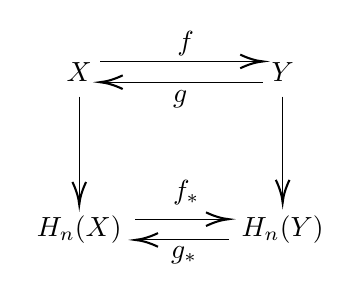
\begin{tikzpicture}[x=0.75pt,y=0.75pt,yscale=-1,xscale=1]
				%uncomment if require: \path (0,300); %set diagram left start at 0, and has height of 300
				
				
				% Text Node
				\draw (271,97) node    {$X$};
				% Text Node
				\draw (369,97) node    {$Y$};
				% Text Node
				\draw (271,173) node    {$H_n( X)$};
				% Text Node
				\draw (369,173) node    {$H_{n}( Y)$};
				% Text Node
				\draw (317,76) node [anchor=north west][inner sep=0.75pt]    {$f$};
				% Text Node
				\draw (315,105) node [anchor=north west][inner sep=0.75pt]    {$g$};
				% Text Node
				\draw (315,148) node [anchor=north west][inner sep=0.75pt]    {$f_{*}$};
				% Text Node
				\draw (314,180) node [anchor=north west][inner sep=0.75pt]    {$g_{*}$};
				% Connection
				\draw    (281,92) -- (357.5,92) ;
				\draw [shift={(359.5,92)}, rotate = 180] [color={rgb, 255:red, 0; green, 0; blue, 0 }  ][line width=0.75]    (10.93,-3.29) .. controls (6.95,-1.4) and (3.31,-0.3) .. (0,0) .. controls (3.31,0.3) and (6.95,1.4) .. (10.93,3.29)   ;
				% Connection
				\draw    (298,168) -- (341,168) ;
				\draw [shift={(343,168)}, rotate = 180] [color={rgb, 255:red, 0; green, 0; blue, 0 }  ][line width=0.75]    (10.93,-3.29) .. controls (6.95,-1.4) and (3.31,-0.3) .. (0,0) .. controls (3.31,0.3) and (6.95,1.4) .. (10.93,3.29)   ;
				% Connection
				\draw    (271,109) -- (271,159) ;
				\draw [shift={(271,161)}, rotate = 270] [color={rgb, 255:red, 0; green, 0; blue, 0 }  ][line width=0.75]    (10.93,-3.29) .. controls (6.95,-1.4) and (3.31,-0.3) .. (0,0) .. controls (3.31,0.3) and (6.95,1.4) .. (10.93,3.29)   ;
				% Connection
				\draw    (369,109) -- (369,158) ;
				\draw [shift={(369,160)}, rotate = 270] [color={rgb, 255:red, 0; green, 0; blue, 0 }  ][line width=0.75]    (10.93,-3.29) .. controls (6.95,-1.4) and (3.31,-0.3) .. (0,0) .. controls (3.31,0.3) and (6.95,1.4) .. (10.93,3.29)   ;
				% Connection
				\draw    (359.5,102) -- (283,102) ;
				\draw [shift={(281,102)}, rotate = 360] [color={rgb, 255:red, 0; green, 0; blue, 0 }  ][line width=0.75]    (10.93,-3.29) .. controls (6.95,-1.4) and (3.31,-0.3) .. (0,0) .. controls (3.31,0.3) and (6.95,1.4) .. (10.93,3.29)   ;
				% Connection
				\draw    (343,178) -- (300,178) ;
				\draw [shift={(298,178)}, rotate = 360] [color={rgb, 255:red, 0; green, 0; blue, 0 }  ][line width=0.75]    (10.93,-3.29) .. controls (6.95,-1.4) and (3.31,-0.3) .. (0,0) .. controls (3.31,0.3) and (6.95,1.4) .. (10.93,3.29)   ;
				
				\end{tikzpicture}
				
			\end{center}
	
		We know that $f\circ g\sim \mathds{1}_x$, which means the induced map $f_*\circ g_*\sim \mathds{1}_{H_n(X)}$. However, according to the last theorem, it is the \textbf{same} map with the identity, so $f_*\circ g_*$ is indeed a isomorphism, so they must both be isomorphism, which finish our proof. 
		
		Now let's prove that theorem. The essential ingredient is a procedure for subdividing the produ ct $\Delta^{n} \times I$ into $(n+1)$ -simplices. The figure shows the cases $n=1,2 .$ In $\Delta^{n} \times I,$ let $\Delta^{n} \times\{0\}=$ $\left[v_{0}, \cdots, v_{n}\right]$ and $\Delta^{n} \times\{1\}=\left[w_{0}, \cdots, w_{n}\right],$ where $v_{i}$ and
		$w_{i}$ have the same image under the projection $\Delta^{n} \times I \rightarrow \Delta^{n}$ The $n$ -simplex $\left[v_{0}, \cdots, v_{i}, w_{i+1}, \cdots, w_{n}\right]$ is the graph of the linear function $\varphi_{i}: \Delta^{n} \rightarrow I$ defined in barycentric coordinates by $\varphi_{i}\left(t_{0}, \cdots, t_{n}\right)=t_{i+1}+\cdots+t_{n}$ since the
		vertices of this simplex $\left[v_{0}, \cdots, v_{i}, w_{i+1}, \cdots, w_{n}\right]$ are on the graph of $\varphi_{i}$ and the simplex projects homeomorphically onto $\Delta^{n}$ under the projection $\Delta^{n} \times I \rightarrow \Delta^{n} .$ The graph of $\varphi_{i}$ lies below the graph of $\varphi_{i-1}$ since $\varphi_{i} \leq \varphi_{i-1}$ and the region between these two graphs is the simplex $\left[v_{0}, \cdots, v_{i}, w_{i}, \cdots, w_{n}\right],$ a true $(n+1)$ -simplex since $w_{i}$ is not on the graph of $\varphi_{i}$ and hence is not in the $n$ -simplex $\left[v_{0}, \cdots, v_{i}, w_{i+1}, \cdots, w_{n}\right]$ From the string of inequalities $0=\varphi_{n} \leq \varphi_{n-1} \leq \cdots \leq \varphi_{0} \leq \varphi_{-1}=1$ we deduce that $\Delta^{n} \times I$ is the union of the $(n+1)$ -simplices $\left[v_{0}, \cdots, v_{i}, w_{i}, \cdots, w_{n}\right],$ each intersecting
		the next in an $n$ -simplex face.
			\begin{center}
				
				
				\tikzset{every picture/.style={line width=0.75pt}} %set default line width to 0.75pt        
				
				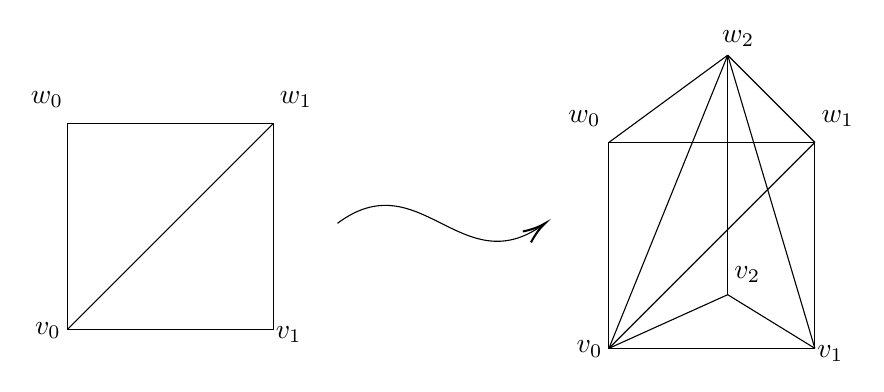
\begin{tikzpicture}[x=0.75pt,y=0.75pt,yscale=-1,xscale=1]
				%uncomment if require: \path (0,300); %set diagram left start at 0, and has height of 300
				
				%Shape: Square [id:dp0581159654904595] 
				\draw   (130.78,94) -- (230,94) -- (230,193.22) -- (130.78,193.22) -- cycle ;
				%Straight Lines [id:da19614555145805979] 
				\draw    (130.78,193.22) -- (230,94) ;
				%Shape: Square [id:dp9902083732035147] 
				\draw   (391.78,103) -- (491,103) -- (491,202.22) -- (391.78,202.22) -- cycle ;
				%Straight Lines [id:da8160304160606769] 
				\draw    (391.78,202.22) -- (491,103) ;
				%Curve Lines [id:da5522177472511686] 
				\draw    (261,142) .. controls (300.6,112.3) and (320.6,170.81) .. (359.81,142.87) ;
				\draw [shift={(361,142)}, rotate = 503.13] [color={rgb, 255:red, 0; green, 0; blue, 0 }  ][line width=0.75]    (10.93,-3.29) .. controls (6.95,-1.4) and (3.31,-0.3) .. (0,0) .. controls (3.31,0.3) and (6.95,1.4) .. (10.93,3.29)   ;
				%Straight Lines [id:da4029878818196849] 
				\draw    (449,61) -- (449,176.38) ;
				%Straight Lines [id:da006355635072525456] 
				\draw    (391.78,202.22) -- (449,176.38) ;
				%Straight Lines [id:da9497079979010515] 
				\draw    (449,176.38) -- (491,202.22) ;
				%Straight Lines [id:da8327026311006851] 
				\draw    (391.78,103) -- (449,61) ;
				%Straight Lines [id:da4087264338700425] 
				\draw    (449,61) -- (491,103) ;
				%Straight Lines [id:da7308100832897756] 
				\draw    (391.78,202.22) -- (449,61) ;
				%Straight Lines [id:da8232160622248595] 
				\draw    (449,61) -- (491,202.22) ;
				
				% Text Node
				\draw (112,77.4) node [anchor=north west][inner sep=0.75pt]    {$w_{0}$};
				% Text Node
				\draw (232,77.4) node [anchor=north west][inner sep=0.75pt]    {$w_{1}$};
				% Text Node
				\draw (114,188.4) node [anchor=north west][inner sep=0.75pt]    {$v_{0}$};
				% Text Node
				\draw (230,190.62) node [anchor=north west][inner sep=0.75pt]    {$v_{1}$};
				% Text Node
				\draw (371,86.4) node [anchor=north west][inner sep=0.75pt]    {$w_{0}$};
				% Text Node
				\draw (493,86.4) node [anchor=north west][inner sep=0.75pt]    {$w_{1}$};
				% Text Node
				\draw (375,197.4) node [anchor=north west][inner sep=0.75pt]    {$v_{0}$};
				% Text Node
				\draw (491,199.62) node [anchor=north west][inner sep=0.75pt]    {$v_{1}$};
				% Text Node
				\draw (451,161.62) node [anchor=north west][inner sep=0.75pt]    {$v_{2}$};
				% Text Node
				\draw (445,48) node [anchor=north west][inner sep=0.75pt]    {$w_{2}$};
				
				
				\end{tikzpicture}
				
			\end{center}
		
		Given a homotopy $F: X \times I \rightarrow Y$ from $f$ to $g$, we can define prism operators $P: C_{n}(X) \rightarrow C_{n+1}(Y) $ by :
			\begin{equation*}
			\begin{aligned}
			P(\sigma)=\sum_{i}(-1)^{i} F \circ(\sigma \times \mathbb{1}) |\left[v_{0}, \cdots, v_{i}, w_{i}, \cdots, w_{n}\right]
			\end{aligned}
			\end{equation*}
			
		for $\sigma: \Delta^{n} \rightarrow X,$ where $F \circ(\sigma \times \mathds{1})$ is the composition $\Delta^{n} \times I \rightarrow X \times I \rightarrow Y .$ We will show
		that these prism operators satisfy the basic relation
			\begin{equation*}
			\begin{aligned}
				\partial P=g_{\#}-f_{\#}-P \partial
			\end{aligned}
			\end{equation*}
			
		Geometrically, the left side of this equation represents the boundary of the prism, and the three terms on the right side represent the top $\Delta^{n} \times\{1\},$ the bottom $\Delta^{n} \times\{0\},$ and the sides $\partial \Delta^{n} \times I$ of the prism. To prove the relation we calculate
			\begin{equation*}
			\begin{aligned}
				\partial P(\sigma)=&\sum_{j \leq i}(-1)^{i}(-1)^{j} F^{\circ}(\sigma \times \mathds{1}) |\left[v_{0}, \cdots, \hat{v}_{j}, \cdots, v_{i}, w_{i}, \cdots, w_{n}\right] \\
				&+\sum_{j \geq i}(-1)^{i}(-1)^{j+1} F^{\circ}(\sigma \times \mathds{1}) |\left[v_{0}, \cdots, v_{i}, w_{i}, \cdots, \widehat{w}_{j}, \cdots, w_{n}\right]
			\end{aligned}
			\end{equation*}
		
		The terms with $i=j$ in the two sums cancel except for $F \circ(\sigma \times \mathds{1}) |\left[\hat{v}_{0}, w_{0}, \cdots, w_{n}\right]$ which is $g \circ \sigma=g_{\#}(\sigma),$ and $-F \circ(\sigma \times \mathds{1}) |\left[v_{0}, \cdots, v_{n}, \widehat{w}_{n}\right],$ which is $-f \circ \sigma=-f_{\neq}(\sigma)$.
		
		The terms with $i \neq j$ are exactly $-P \partial(\sigma)$ since
			\begin{equation*}
			\begin{aligned}
				P \partial(\sigma)=&\sum_{i<j}(-1)^{i}(-1)^{j} F_{\circ}(\sigma \times \mathds{1}) |\left[v_{0}, \cdots, v_{i}, w_{i}, \cdots, \widehat{w}_{j}, \cdots, w_{n}\right] \\
				&+\sum_{i>j}(-1)^{i-1}(-1)^{j} F_{0}(\sigma \times \mathds{1}) |\left[v_{0}, \cdots, \hat{v}_{j}, \cdots, v_{i}, w_{i}, \cdots, w_{n}\right]
			\end{aligned}
			\end{equation*}
			
		Now we can finish the proof of the theorem. If $\alpha \in C_{n}(X)$ is a cycle, then we have $g_{\neq}(\alpha)-f_{\#}(\alpha)=\partial P(\alpha)+P \partial(\alpha)=\partial P(\alpha)$ since $\partial \alpha=0 .$ Thus $g_{\neq}(\alpha)-f_{\#}(\alpha)$ is
		a boundary, so $g_{\#}(\alpha)$ and $f_{\#}(\alpha)$ determine the same homology class, which means that $g_{*}$ equals $f_{*}$ on the homology class of $\alpha$. 
		
	\subsection{Exercise 5.32}
		Consider $\forall c\in C^p, c\neq 0$, we have
			\begin{equation*}
			\begin{aligned}
				&\Delta_p c=0\\
				\Rightarrow  &\left\langle \Delta_pc,c\right\rangle_{g_p^{-1}}=0\\
				\Rightarrow  &\left\langle (\delta^*_{p+1}\delta_p+\delta_{p-1}\delta^*_p)c,c\right\rangle_{g_p^{-1}}=0\\
				\Rightarrow &\left\langle\delta_pc,\delta_pc\right\rangle_{g_p^{-1}}+\left\langle\delta_p^*c,\delta_p^*c\right\rangle_{g_p^{-1}}=0
			\end{aligned}
			\end{equation*}
			
		But we know that the inner product is positive definite, which means $\delta_pc=0$ and $\delta_p^*c=0$. 
		
		For the opposite direction, if we know that $\delta_pc=0$ and $\delta_p^*c=0$, thus $\Delta_pc=\delta^*_{p+1}\delta_pc+\delta_{p-1}\delta^*_pc=\delta^*_{p+1}0+\delta_{p-1}0=0$, thus our proof finishes. 
		
	\subsection{Exercise 5.33}
		Consider the boundary homomorphism,
			\begin{equation*}
			\begin{aligned}
				\partial_{r}: C_{r}(K ; \mathbb{R}) \rightarrow C_{r-1}(K ; \mathbb{R})
			\end{aligned}
			\end{equation*}
			
		Where $C_{-1}(K ; \mathbb{R})$ is defined to be $\{0\} .$ since both $C_{r-1}(K ; \mathbb{R})$ and $C_{r}(K ; \mathbb{R})$ are vector spaces, according to the fundamental theorem of linear map:
			\begin{equation*}
			\begin{aligned}
			I_{r} &=\operatorname{dim} C_{r}(K ; \mathbb{R})=\operatorname{dim}\left(\operatorname{ker} \partial_{r}\right)+\operatorname{dim}\left(\operatorname{im} \partial_{r}\right) \\
			&=\operatorname{dim} Z_{r}(K ; \mathbb{R})+\operatorname{dim} B_{r-1}(K ; \mathbb{R})
			\end{aligned}
			\end{equation*}
			
		Where $B_{-1}(K)$ is defined to be trivial. We also have
			\begin{equation*}
			\begin{aligned}
				b_{r}(K) &=\operatorname{dim} H_{r}(K ; \mathbb{R})=\operatorname{dim}\left(Z_{r}(K ; \mathbb{R}) / B_{r}(K ; \mathbb{R})\right) \\
				&=\operatorname{dim} Z_{r}(K ; \mathbb{R})-\operatorname{dim} B_{r}(K ; \mathbb{R})
			\end{aligned}
			\end{equation*}
			
		From these relations, we obtain:
			\begin{equation*}
			\begin{aligned}
				\chi(K) &=\sum_{r=0}^{n}(-1)^{r} b_{r}(K)\\
				&=\sum_{r=0}^{n}\left\{(-1)^{r} \operatorname{dim} Z_{r}(K ; \mathbb{R})-(-1)^{r} \operatorname{dim} B_{r}(K ; \mathbb{R})\right\} \\
				&=\sum_{r=0}^{n}(-1)^{r}\left(\operatorname{dim} Z_{r}(K ; \mathbb{R})+\operatorname{dim} B_{r-1}(K ; \mathbb{R})\right) \\
				&=\sum_{r=0}^{n}(-1)^{r} I_{r}=\operatorname{dim} C_{r}(K ; \mathbb{R})\\
			\end{aligned}
			\end{equation*}
			
	\subsection{Exercise 5.34}
		As the figure shows: 
			\begin{center}
				
				
				\tikzset{every picture/.style={line width=0.75pt}} %set default line width to 0.75pt        
				
				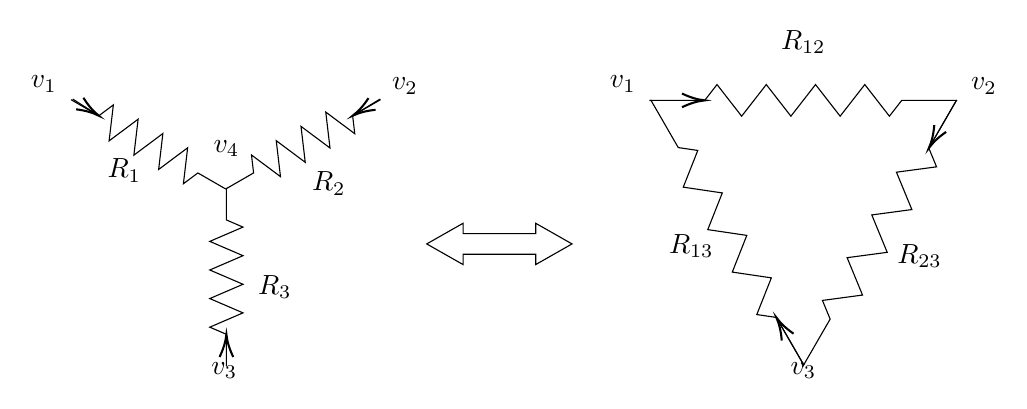
\begin{tikzpicture}[x=0.75pt,y=0.75pt,yscale=-1,xscale=1]
				%uncomment if require: \path (0,300); %set diagram left start at 0, and has height of 300
				
				%Shape: Resistor [id:dp7919219813839989] 
				\draw   (221.16,130.11) -- (234.58,122.37) -- (233.56,113.71) -- (247.53,124.14) -- (245.49,106.82) -- (259.46,117.25) -- (257.42,99.93) -- (271.39,110.36) -- (269.35,93.05) -- (283.32,103.47) -- (282.3,94.82) -- (295.72,87.07) ;
				%Shape: Resistor [id:dp13218154183477826] 
				\draw   (146.61,87.07) -- (160.03,94.82) -- (167.01,89.6) -- (164.97,106.92) -- (178.94,96.49) -- (176.9,113.81) -- (190.87,103.38) -- (188.83,120.69) -- (202.8,110.26) -- (200.76,127.58) -- (207.74,122.37) -- (221.16,130.11) ;
				%Shape: Resistor [id:dp05970520604034513] 
				\draw   (221.48,129.52) -- (221.48,145.02) -- (229.48,148.46) -- (213.47,155.35) -- (229.48,162.24) -- (213.47,169.13) -- (229.48,176.01) -- (213.47,182.9) -- (229.48,189.79) -- (213.47,196.68) -- (221.48,200.12) -- (221.48,215.62) ;
				%Straight Lines [id:da17529824233424984] 
				\draw    (147.41,86.76) -- (158.34,93.74) ;
				\draw [shift={(160.03,94.82)}, rotate = 212.55] [color={rgb, 255:red, 0; green, 0; blue, 0 }  ][line width=0.75]    (10.93,-3.29) .. controls (6.95,-1.4) and (3.31,-0.3) .. (0,0) .. controls (3.31,0.3) and (6.95,1.4) .. (10.93,3.29)   ;
				%Straight Lines [id:da07945999998264752] 
				\draw    (221.48,215.62) -- (221.48,202.12) ;
				\draw [shift={(221.48,200.12)}, rotate = 450] [color={rgb, 255:red, 0; green, 0; blue, 0 }  ][line width=0.75]    (10.93,-3.29) .. controls (6.95,-1.4) and (3.31,-0.3) .. (0,0) .. controls (3.31,0.3) and (6.95,1.4) .. (10.93,3.29)   ;
				%Straight Lines [id:da5636992361849839] 
				\draw    (295.54,86.76) -- (284.01,93.78) ;
				\draw [shift={(282.3,94.82)}, rotate = 328.69] [color={rgb, 255:red, 0; green, 0; blue, 0 }  ][line width=0.75]    (10.93,-3.29) .. controls (6.95,-1.4) and (3.31,-0.3) .. (0,0) .. controls (3.31,0.3) and (6.95,1.4) .. (10.93,3.29)   ;
				%Shape: Resistor [id:dp3001006918460648] 
				\draw   (498.98,215.96) -- (512.36,192.79) -- (508.65,183.79) -- (527.96,181.21) -- (520.54,163.2) -- (539.85,160.62) -- (532.43,142.6) -- (551.73,140.02) -- (544.31,122.01) -- (563.62,119.43) -- (559.91,110.43) -- (573.29,87.26) ;
				%Shape: Resistor [id:dp601959072653126] 
				\draw   (425.23,87.41) -- (451.93,87.41) -- (457.86,79.79) -- (469.72,95.03) -- (481.59,79.79) -- (493.45,95.03) -- (505.32,79.79) -- (517.18,95.03) -- (529.05,79.79) -- (540.91,95.03) -- (546.85,87.41) -- (573.54,87.41) ;
				%Shape: Resistor [id:dp987133647106214] 
				\draw   (425.89,87.13) -- (439.18,110.15) -- (448.59,111.54) -- (441.59,129.22) -- (460.4,132) -- (453.4,149.68) -- (472.21,152.46) -- (465.21,170.14) -- (484.03,172.92) -- (477.02,190.6) -- (486.43,191.99) -- (499.72,215.01) ;
				%Straight Lines [id:da5845488205382635] 
				\draw    (425.41,87.41) -- (449.93,87.41) ;
				\draw [shift={(451.93,87.41)}, rotate = 180] [color={rgb, 255:red, 0; green, 0; blue, 0 }  ][line width=0.75]    (10.93,-3.29) .. controls (6.95,-1.4) and (3.31,-0.3) .. (0,0) .. controls (3.31,0.3) and (6.95,1.4) .. (10.93,3.29)   ;
				%Straight Lines [id:da8280931053411327] 
				\draw    (499.72,215.01) -- (487.43,193.72) ;
				\draw [shift={(486.43,191.99)}, rotate = 420] [color={rgb, 255:red, 0; green, 0; blue, 0 }  ][line width=0.75]    (10.93,-3.29) .. controls (6.95,-1.4) and (3.31,-0.3) .. (0,0) .. controls (3.31,0.3) and (6.95,1.4) .. (10.93,3.29)   ;
				%Straight Lines [id:da29329043154429146] 
				\draw    (573.29,87.26) -- (560.91,108.7) ;
				\draw [shift={(559.91,110.43)}, rotate = 300] [color={rgb, 255:red, 0; green, 0; blue, 0 }  ][line width=0.75]    (10.93,-3.29) .. controls (6.95,-1.4) and (3.31,-0.3) .. (0,0) .. controls (3.31,0.3) and (6.95,1.4) .. (10.93,3.29)   ;
				%Left Right Arrow [id:dp7783077363277054] 
				\draw   (318,156.57) -- (335.5,146.62) -- (335.5,151.59) -- (370.5,151.59) -- (370.5,146.62) -- (388,156.57) -- (370.5,166.52) -- (370.5,161.54) -- (335.5,161.54) -- (335.5,166.52) -- cycle ;
				
				% Text Node
				\draw (126,74.4) node [anchor=north west][inner sep=0.75pt]    {$v_{1}$};
				% Text Node
				\draw (300,75.4) node [anchor=north west][inner sep=0.75pt]    {$v_{2}$};
				% Text Node
				\draw (214,105.4) node [anchor=north west][inner sep=0.75pt]    {$v_{4}$};
				% Text Node
				\draw (213,212.4) node [anchor=north west][inner sep=0.75pt]    {$v_{3}$};
				% Text Node
				\draw (405,74.4) node [anchor=north west][inner sep=0.75pt]    {$v_{1}$};
				% Text Node
				\draw (579,75.4) node [anchor=north west][inner sep=0.75pt]    {$v_{2}$};
				% Text Node
				\draw (492,212.4) node [anchor=north west][inner sep=0.75pt]    {$v_{3}$};
				% Text Node
				\draw (163,114.4) node [anchor=north west][inner sep=0.75pt]    {$R_{1}$};
				% Text Node
				\draw (261.46,120.65) node [anchor=north west][inner sep=0.75pt]    {$R_{2}$};
				% Text Node
				\draw (235.46,170.65) node [anchor=north west][inner sep=0.75pt]    {$R_{3}$};
				% Text Node
				\draw (487.46,52.65) node [anchor=north west][inner sep=0.75pt]    {$R_{12}$};
				% Text Node
				\draw (433.46,150.65) node [anchor=north west][inner sep=0.75pt]    {$R_{13}$};
				% Text Node
				\draw (543.46,155.65) node [anchor=north west][inner sep=0.75pt]    {$R_{23}$};
				
				
				\end{tikzpicture}
				
			\end{center}
		
		We first consider the $Y$ graph. To figure out its boundary operator, we need to find it chain group:
			\begin{equation*}
			\begin{aligned}
				&C_0=\operatorname{Span}\{v_1,v_2,v_3,v_4\}\\
				&C_1=\operatorname{Span}\{i_1,i_2,i_3\}
			\end{aligned}
			\end{equation*}
		
		We know that $C_1\xlongrightarrow[]{\pa_1}C_0$, which means:
			\begin{equation*}
			\begin{aligned}
			\pa_1=
				\begin{pmatrix}
					-1 & 0 & 0\\
					0 & -1 & 0\\
					0 & 0 & -1\\
					1 & 1 & 1
				\end{pmatrix}
			\end{aligned}
			\end{equation*}
			
		For example:
			\begin{equation*}
			\begin{aligned}
				pa_1i_1=
				\begin{pmatrix}
					-1 & 0 & 0\\
					0 & -1 & 0\\
					0 & 0 & -1\\
					1 & 1 & 1
				\end{pmatrix}
				\begin{pmatrix}
					1\\
					0\\
					0
				\end{pmatrix}
				=
				\begin{pmatrix}
					-1\\
					0\\
					0\\
					1
				\end{pmatrix}=v_4-v_1
			\end{aligned}
			\end{equation*}
			
		For cocycles, we also have:
			\begin{equation*}
			\begin{aligned}
				C^0&=\operatorname{Span}\{\phi_1,\phi_2,\phi_3\}\\
				C^1&=\operatorname{Span}\{u_1,u_2,u_3,u_4\}\\
				&C^0\xlongrightarrow[]{\delta_0}C^1
			\end{aligned}
			\end{equation*}
			
		So the coboundary operator looks like:
			\begin{equation*}
			\begin{aligned}
			\delta_0=
				\begin{pmatrix}
					-1 & 0 & 0 & 1\\
					0 & -1 & 0 & 1\\
					0 & 0 & -1 & 1
				\end{pmatrix}
			\end{aligned}
			\end{equation*}
			
		The metric turn a 1-cycle to a 1-cocycle($u=Ri$):
			\begin{equation*}
			\begin{aligned}
				R=
				\begin{pmatrix}
					R_1 & 0 & 0\\
					0 & R_2 & 0\\
					0 & 0 & R_3
				\end{pmatrix}
			\end{aligned}
			\end{equation*}
			
		The Laplacian is then:
			\begin{equation*}
			\begin{aligned}
				\Delta=\delta_{1}^{*} \delta_{0}=\partial_{1} \cdot R^{-1} \cdot \delta_{0}=\left(\begin{array}{ccc}
				-R_{1}^{-1} & 0 & 0 \\
				0 & -R_{2}^{-1} & 0 \\
				0 & 0& -R_{3}^{-1} \\
				R_{1}^{-1} & R_{2}^{-1} & R_{3}^{-1}
				\end{array}\right) \cdot \delta_{0}=\left(\begin{array}{cccc}
				R_{1}^{-1} & 0 & 0 & -R_{1}^{-1} \\
				0 & R_{2}^{-1} & 0 & -R_{2}^{-1} \\
				0 & 0 & R_{3}^{-1} & -R_{3}^{-1} \\
				-R_{1}^{-1}&-R_{2}^{-1}&-R_{3}^{-1} & R_{1}^{-1}+R_{2}^{-1}+R_{3}^{-1}
				\end{array}\right)
			\end{aligned}
			\end{equation*}
			
		We require that $\Delta \vec{\phi}-\vec{i}$, which means:
			\begin{equation*}
			\begin{aligned}
				\left\{\begin{array}{l}
				R_{1}^{-1}\left(\phi_{1}-\phi_{4}\right)=-i_{1} \\
				R_{2}^{-1}\left(\phi_{2}-\phi_{4}\right)=-i_{2} \\
				R_{3}^{-1}\left(\phi_{3}-\phi_{4}\right)=-i_{3} \\
				i_{1}+i_{2}+i_{3}=0
				\end{array}\right.
			\end{aligned}
			\end{equation*}
			
		We can compute that:
			\begin{equation*}
			\begin{aligned}
				\phi_4=\frac{R_{1}^{-1} \phi_{1}+R_{2}^{-1} \phi_{2}+R_{3}^{-1} \phi_{3}}{R_{2}^{-1}+R_{2}^{-1}+R_{3}^{-1}}
			\end{aligned}
			\end{equation*}
			
		Define that: $Y_i=R_i^{-1}$, then the relation between $\phi$ and $i$ becomes:
			\begin{equation*}
			\begin{aligned}
				\frac{1}{Y_{1}+Y_{2}+Y_{3}}\left(\begin{array}{ccc}
				Y_{1}\left(Y_{2}+Y_{3}\right) & -Y_{1} Y_{2} & -Y_{1} Y_{3} \\
				-Y_{1} Y_{2} & Y_{2}\left(Y_{1}+Y_{3}\right) & -Y_{2} Y_{3} \\
				-Y_{1} Y_{3} & -Y_{2} Y_{3} & Y_{3}\left(Y_{1}+Y_{2}\right)
				\end{array}\right)\left(\begin{array}{l}
				\phi_{1} \\
				\phi_{2} \\
				\phi_{3}
				\end{array}\right)=-\left(\begin{array}{c}
				i_{1} \\
				i_{2} \\
				i_{3}
				\end{array}\right)
			\end{aligned}
			\end{equation*}
			
		For the second graph, we have:
			\begin{equation*}
			\begin{aligned}
				\partial_{1}=\left(\begin{array}{ccc}
				-1 & 0 & 1 \\
				1 & -1 & 0 \\
				0 & 1 & -1
				\end{array}\right) \quad \delta_{0}=\left(\begin{array}{ccc}
				-1 & 1 & 0 \\
				0 & -1 & 1 \\
				1 & 0 & -1
				\end{array}\right) \quad R^{-1}=\left(\begin{array}{ccc}
				Y_{12} & 0 & 0 \\
				0 & Y_{23} & 0 \\
				0 & 0 & Y_{31}
				\end{array}\right)
			\end{aligned}
			\end{equation*}
			
		The laplacian looks like:
			\begin{equation*}
			\begin{aligned}
				\Delta=\partial_{1} \circ R^{-1} \circ \delta_{0}=\left(\begin{array}{ccc}
				-Y_{12} & 0 & Y_{31} \\
				Y_{12} & -Y_{23} & 0 \\
				0 & Y_{23} & -Y_{31}
				\end{array}\right) \cdot \delta_{0}=\left(\begin{array}{cccc}
				Y_{12}+Y_{31} & -Y_{12} & -Y_{31} \\
				-Y_{12} & Y_{12}+Y_{23} & -Y_{23} \\
				-Y_{31} & -Y_{23} & Y_{31}+Y_{32}
				\end{array}\right)
			\end{aligned}
			\end{equation*}
			
		We must impose $\Delta \vec{\phi}=-\vec{i}$, compare two matrix coeffienct of the equation $\Delta \vec{\phi}=-\vec{i}$, we have:
			\begin{equation*}
			\begin{aligned}
				\begin{cases}
					\frac{Y_{1} Y_{2}}{Y_{1}+Y_{2}+Y_{3}}=Y_{12}\\
					\frac{Y_{1} Y_{3}}{Y_{1}+Y_{2}+Y_{3}}=Y_{31} \\
					\frac{Y_{2} Y_{3}}{Y_{1}+Y_{2}+Y_{3}}=Y_{23}
				\end{cases}
			\end{aligned}
			\end{equation*}
			
		Which means:
			\begin{equation*}
			\begin{aligned}
				\left\{\begin{array}{l}
				R_{12}=\frac{R_{1} R_{2}+R_{1} R_{3}+R_{2} R_{3}}{R_{3}} \\
				R_{13}=\frac{R_{1} R_{2}+R_{1} R_{3}+R_{2} R_{3}}{R_{2}} \\
				R_{23}=\frac{R_{1} R_{2}+R_{1} R_{3}+R_{2} R_{3}}{R_{1}}
				\end{array}\right.
			\end{aligned}
			\end{equation*}
		
		This is the relation of the resistant between two graphs. 
		
\section{Complex intergation}
	\subsection{Exercise 6.1}
	Consider the product $S=w_0w_0'+(w_0w_1'+w_1w_0')+(w_0w_2'+w_1w_1'+w_2w_0')+\cdots$, i.e., 
	\begin{equation*}
	S=\sum_{n=0}^\infty A_n,\;\;A_n=\sum_{j=0}^nw_jw_{n-j}'
	\end{equation*}
	We can prove that $A_0+A_1+\cdots$ is absolutely convergent. Let 
	\begin{equation*}
	\sigma_N\equiv\sum_{n=0}^N|A_n|
	\end{equation*}
	As $\sigma_N$ is increasing and $\sigma_N$ is bounded above, the sequence $\{\sigma_N\}$ is converge, and thus $\sum_{n=0}^\infty|A_n|$ is convergent, i.e., 
	$S=\sum_{n=0}^\infty A_n$ is absolutely convergent. Therefore, the result of the product $(\sum_jw_j)(\sum_jw_j')$ is independent of the order of the summation, and 
	thus $(\sum_jw_j)(\sum_jw_j')=S$ is absolutely convergent. 
	\subsection{Exercise 6.2}
	Without loss of generality, let $R_a>R_b$. The radius of the convergence is given by 
	\begin{equation*}
	R=\lim_{j\to\infty}\frac{1}{|a_j+b_j|^{1/j}}
	\end{equation*}
	Noting that 
	\begin{equation*}
	\lim_{j\to\infty}\left|\frac{a_j}{b_j}\right|^{1/j}=\frac{R_b}{R_a}\ne 1\;\;\Rightarrow\;\;\lim_{j\to\infty}\left|\frac{a_j}{b_j}\right|=0
	\end{equation*}
	we have 
	\begin{equation*}
	R=\lim_{j\to\infty}\frac{1}{|b_j|^{1/j}}\lim_{j\to\infty}\frac{1}{|1+a_j/b_j|^{1/j}}=R_b
	\end{equation*}
	Similarly, for the second series, we also have $R=R_b$. For the rest two series, by definition, its easy to show that $R=R_aR_b$ and $R=R_a/R_b$ respectively. 
	\subsection{Exercise 6.3}
	The (6.2) in the Lecture notes gives 
	\begin{equation*}
	\oint_\ell f(z)\mathrm{d}z=-\iint\left(\frac{\partial v}{\partial x}+\frac{\partial u}{\partial y}\right)\mathrm{d}x\mathrm{d}y+\mathrm{i}\iint\left(\frac{\partial u}{\partial x}-\frac{\partial v}{\partial y}\right)\mathrm{d}x\mathrm{d}y\equiv 0
	\end{equation*}
	As for all the loop $\ell\subset R$ the integral vanishes, we must have 
	\begin{equation*}
	\frac{\partial v}{\partial x}+\frac{\partial u}{\partial y}\equiv 0\;\;\text{and}\;\;\frac{\partial u}{\partial x}-\frac{\partial v}{\partial y}\equiv 0\;\;\text{when}\;z\in R
	\end{equation*}
	i.e., $f(z)$ is holomorphic in $R$. 
	\subsection{Exercise 6.4}
	The coordinate transformation $(x,y)\to(z,\bar z)$ gives the Jacobian matrix: 
	\begin{equation*}
	\begin{pmatrix}
	\mathrm{d}z\\\mathrm{d}\bar z
	\end{pmatrix}=\begin{pmatrix}
	1 & \mathrm{i} \\ 1 & -\mathrm{i}
	\end{pmatrix}\begin{pmatrix}
	\mathrm{d}x \\ \mathrm{d}y
	\end{pmatrix}
	\end{equation*}
	Therefore we have 
	\begin{equation*}
	\partial=\frac 12(\partial_x-\mathrm{i}\partial_y),\;\;\bar\partial=\frac 12(\partial_x+\mathrm{i}\partial_y)
	\end{equation*}
	and the metric in $(z,\bar z)$ is given by 
	\begin{equation*}
	g'=\begin{pmatrix}
	0 & 1/2\\
	1/2 & 0
	\end{pmatrix}
	\end{equation*}
	The integral measure is given by 
	\begin{equation*}
	\mathrm{d}z\wedge\mathrm{d}\bar z=\sqrt{|g'|}(\mathrm{d}x+\mathrm{i}\mathrm{d}y)\wedge(\mathrm{d}x-\mathrm{i}\mathrm{d}y)=\frac{\mathrm{i}}{2}\mathrm{d}x\wedge\mathrm{d}y
	\end{equation*}
	\subsection{Exercise 6.5}
	The solution will be construct soon. 
	\subsection{Exercise 6.6}
	The solution will be construct soon. 
	\subsection{Exercise 6.7}
	For $f(z)=z^2$, let $z_j=\mathrm{e}^{\mathrm{i}2\uppi j/N}$, then $\Delta_j=z_{j+1}-z_j$ and 
	\begin{equation*}
	w_j\Delta_j=(\mathrm{e}^{\mathrm{i}2\uppi j/N})^2(\mathrm{e}^{\mathrm{i}2\uppi (j+1)/N}-\mathrm{e}^{\mathrm{i}2\uppi j/N})=\mathrm{e}^{\mathrm{i}2\uppi(3j)/N}(\mathrm{e}^{\mathrm{i}2\uppi/N}-1)
	\end{equation*}
	The term in the bracket is a constant vector. Therefore, 
	\begin{equation*}
	\oint z^2\mathrm{d}z=\lim_{N\to\infty}\sum_{j=0}^{N-1}w_j\Delta_j\propto\lim_{N\to\infty}\sum_{j=0}^{N-1}\mathrm{e}^{\mathrm{i}2\uppi (3j)/N}=0
	\end{equation*}
	\subsection{Exercise 6.8}
	For $f(z)=z^{-2}$, let $z_j=\mathrm{e}^{\mathrm{i}2\uppi j/N}$, then $\Delta_j=z_{j+1}-z_j$ and 
	\begin{equation*}
	w_j\Delta_j=(\mathrm{e}^{-\mathrm{i}2\uppi j/N})^2(\mathrm{e}^{\mathrm{i}2\uppi (j+1)/N}-\mathrm{e}^{\mathrm{i}2\uppi j/N})=\mathrm{e}^{-\mathrm{i}2\uppi j/N}(\mathrm{e}^{\mathrm{i}2\uppi/N}-1)
	\end{equation*}
	The term in the bracket is a constant vector. Therefore, 
	\begin{equation*}
	\oint z^2\mathrm{d}z=\lim_{N\to\infty}\sum_{j=0}^{N-1}w_j\Delta_j\propto\lim_{N\to\infty}\sum_{j=0}^{N-1}\mathrm{e}^{-\mathrm{i}2\uppi j/N}=0
	\end{equation*}
	\subsection{Exercise 6.9}
	\subsection{Exercise 6.10}
	According to the Gauss mean value theorem, given a function $f(z),$ holomorphic on and inside a circle $C_{r}$ centered at $a,$ since $f(a)$ is the mean value of $f(z)$ on $C_{r},$ there must exist a point on $a^{\prime} \in C_{r}$ with $\left|f\left(a^{\prime}\right)\right|<|f(a)| .$ We can examine this thought more carefully. Suppose $f(z)$ is holomorphic on and inside a loop (not necessarily a circle) $l$, as in the Figure 6.10 in the note. Take a generic point $a$ inside $l$ and draw an infinitesimal circle $C_{\varepsilon}$ of radius $\varepsilon$ centered at $a$. Then $\exists a^{\prime} \in C_{\varepsilon},$ such that $\left|f\left(a^{\prime}\right)\right|<|f(a)|$ and $\left|f\left(a^{\prime}\right)\right|$ is the maximal one on $C_{\varepsilon}$. The modulus $\left|f^{\prime}(a)\right|$ is in fact the largest on the entire small disk bounded by $C_{\varepsilon}$ because the infinitesimal disk is mapped to another infinitesimal disk centered at $f(a)$ with radius $\left|f^{\prime}(a)\right| \varepsilon .$ The modulus of the points in on this image disk can take mininal value only on the boundary. Now draw another circle $C_{\varepsilon}^{\prime}$ centered at $a^{\prime}$. Then, $\exists a^{\prime \prime} \in C_{\epsilon}^{\prime}$, such
	that $\left|f\left(a^{\prime \prime}\right)\right|<\left|f\left(a^{\prime}\right)\right|$ and is the maximum on $C_{\varepsilon}^{\prime}$. This $a^{\prime \prime}$ must not lie on $C_{\varepsilon}$ because $\left|f\left(a^{\prime}\right)\right|$ is the minimum on $C_{\varepsilon} .$ This procedure can be continued until the new $n$-th circle $C_{\varepsilon}^{(n)}$ touches $l$ tangentially at some point $b \in l$ (this can always be achieved by adjusting the radius $\varepsilon$). Finally, we take the limit $\varepsilon \rightarrow 0\;(n \rightarrow \infty)$, which brings the sequence of points $a, a^{\prime}, a^{\prime \prime}, \ldots, a^{(n)}, b$ infinitely close to each other. We have $|f(b)|<\left|f\left(a^{n}\right)\right|<\cdots<|f(a)|$. Since $a$ is arbitrary, for any $a$, there is such a sequence of points reaching some $b \in l$ with $|f(b)|$ is the minimal along the sequence. We can conclude that the maximum of $|f(z)|$ can only exist on $l$. 
	\subsection{Exercise 6.11}
	The Taylor expansion of $\mathrm{e}^z$ is:
	\begin{equation*}
	\mathrm{e}^{z}=\sum_{n=0}^\infty\frac{z^n}{n!},\;\;R=\infty
	\end{equation*}
	
	The Taylor expansion of $\sin^2z$ is:
	\begin{equation*}
	\sin^2 z=-\frac{\mathrm{e}^{2\mathrm{i}z}+\mathrm{e}^{-2\mathrm{i}z}-2}{4}=\frac 12-\frac 14\sum_{n=0}^\infty\frac{(2\mathrm{i})^n}{n!}(1+(-1)^n)z^n=\frac 12-\frac 12\sum_{k=0}^\infty\frac{(2\mathrm{i})^{2k}}{(2k)!}z^{2k},\;\;R=\infty
	\end{equation*}
	and the Taylor expansion of $\cos^2z$ is given by $1-\sin^2z$ with $R=\infty$. 
	
	The Taylor expansion of $\ln z$ around $z=1$ is 
	\begin{equation*}
	\ln z=\sum_{n=1}^\infty\frac{(-1)^{n-1}}{n}(z-1)^n,\;\;R=1
	\end{equation*}
	and the Taylor expansion of $\ln z$ around $z=\mathrm{i}$ is 
	\begin{equation*}
	\ln z=\frac{\mathrm{i}\uppi}{2}+\sum_{n=1}^\infty\frac{\mathrm{i}^{n-2}}{n}(z-\mathrm{i})^n,\;\;R=1
	\end{equation*}
	
	The Taylor expansion of $\sqrt{1+z^2}$ around $z=0$ is 
	\begin{equation*}
	\sqrt{1+z^2}=\sum_{n=0}^\infty\frac{1}{n!}\frac{(-1)^{n-1}}{2^n}(2n-3)!!z^{2n}
	\end{equation*}
	The radius of convergence is 
	\begin{equation*}
	R=\lim_{n\to\infty}\frac{\dfrac{1}{n!}\dfrac{1}{2^n}(2n-3)!!}{\dfrac{1}{(n+1)!}\dfrac{1}{2^{n+1}}(2n-1)!!}=\lim_{n\to\infty}\frac{2(n+1)}{2n-1}=1
	\end{equation*}
	
	To find the Taylor expansion of $\arctan z$ around $z=0$, consider the Taylor expansion of $1/(1+z^2)$: 
	\begin{equation*}
	\frac{1}{1+z^2}=\sum_{n=0}^\infty(-1)^nz^{2n}
	\end{equation*}
	Therefore, 
	\begin{equation*}
	\arctan z=\int_0^z\frac{\mathrm{d}\zeta}{1+\zeta^2}=\sum_{n=0}^\infty(-1)^n\frac{1}{2n+1}z^{2n+1},\;\;R=1
	\end{equation*}
	
	It's hard to write a general expression for the coefficients of the Taylor expansion of $(1+z)^{1/z}$ around $z=0$. For the first few orders of this series, we have 
	\begin{equation*}
	(1+z)^{1/z}=\mathrm{e}\left(1-\frac z2+\frac{11}{24}z^2-\frac 7{16}z^3+\frac{2447}{5760}z^4+\mathcal O(z^5)\right)
	\end{equation*}
	\subsection{Exercise 6.12}
	It's also hard to find the general expression for the coefficients of the Taylor expansion of $1/(2-\sin z)$. For the first few orders of this series, we have 
	\begin{equation*}
	\frac{1}{2-\sin z}=\frac 12+\frac z4+\frac{z^2}{8}+\frac{z^3}{48}-\frac{z^4}{96}-\frac{13z^5}{960}+\mathcal{O}(z^6)
	\end{equation*}
	To find the radius of convergence, just consider the equation: 
	\begin{equation*}
	\sin z_0=\frac{\mathrm{e}^{\mathrm{i}z_0}-\mathrm{e}^{-\mathrm{i}z_0}}{2\mathrm{i}}=2\;\;\Rightarrow\;\;z_0=\frac{\uppi}{2}+2k\uppi+\mathrm{i}\ln(2\pm\sqrt{3}),\;\;k\in\mathbb Z
	\end{equation*}
	Then we have 
	\begin{equation*}
	R=\inf_{k\in\mathbb Z}\{|z_0|\}=\sqrt{\frac{\uppi^2}{4}+\big[\ln(2+\sqrt{3})\big]^2}
	\end{equation*}
	\subsection{Exercise 6.13}
	For the “$\Rightarrow$”: Let 
	\begin{equation*}
	g(z)=\sum_{k=m}^{\infty}a_k(z-z_0)^{k-m}
	\end{equation*}
	As $f(z)=\sum_{k=m}^\infty a_k(z-z_0)^k$ is convergent in $R$, $g(z)$ must also be convergent in $R$ and $g(z_0)=a_m\ne 0$. Then we have $f(z)=(z-z_0)^m g(z)$. 
	
	For the “$\Leftarrow$”: As $g(z_0)\ne 0$, we can expand $g(z)$ at $z=z_0$ as 
	\begin{equation*}
	g(z)=\sum_{k=0}^\infty b_k(z-z_0)^k
	\end{equation*}
	with $b_0\ne 0$. Then 
	\begin{equation*}
	f(z)=\sum_{k=0}^\infty b_k(z-z_0)^{m+k}=\sum_{k=m}^\infty a_k(z-z_0)^k,\;\;a_k=b_{k-m}
	\end{equation*}
	
	To prove that $z_0$ is an isolated zero of $f(z)$, consider $z\ne z_0$ with $f(z)=0$. Then we have $g(z)=0$. If $\forall\delta>0$ s.t. $\exists z\in U(z_0,\delta)$ s.t. $f(z)=0$, we have 
	$\lim_{z\to z_0}g(z)=0=g(z_0)$, which is contradictory with our assumption $g(z_0)\ne 0$. 
	
	\subsection{Exercise 6.14}
	Define $G_n(t)$ s.t. $f(z)=\mathrm{e}^{2tz-z^2}=\sum_{n=0}^\infty G_n(t)z^n/n!$, then we have 
	\begin{equation*}
	G_0(t)=H_0(t)=1\;\;G_1(t)=H_1(t)=2t,\;\;G_2(t)=H_2(t)=4t^2-2
	\end{equation*}
	Therefore, it's sufficient to prove that sequences $\{H_n\}$ and $\{G_n\}$ satisfy the same form of the recurrence relation. First we derive the recurrence relation of 
	$H_n(t)$: 
	\begin{equation*}
	H_{n+1}(t)=(-1)^{n+1}\me^{t^2}\frac{\mathrm{d}}{\mathrm{d}t}\frac{\mathrm{d}^n}{\mathrm{d}t^n}\mathrm{e}^{-t^2}=(-1)^{n+1}\mathrm{e}^{t^2}\frac{\mathrm{d}}{\mathrm{d}t}(-1)^n\mathrm{e}^{-t^2}H_n(t)
	\end{equation*}
	Then 
	\begin{equation*}
	H_{n+1}(t)=2tH_n(t)-H_n'(t)
	\end{equation*}
	This is our recurrence relation. 
	
	The expression of $G_n(t)$ is given by: 
	\begin{equation*}
	f(z)=\sum_{n=0}^\infty\sum_{m=0}^\infty\frac{1}{n!}\frac{(-1)^m}{m!}(2t)^nz^{n+2m}\xlongrightarrow[]{k=n+2m}\sum_{k=0}^\infty\sum_{m=0}^{[k/2]}\frac{1}{(k-2m)!}\frac{(-1)^m}{m!}(2t)^{k-2m}z^k
	\end{equation*}
	Therefore 
	\begin{equation*}
	G_n(t)=n!\sum_{m=0}^{[n/2]}\frac{1}{(n-2m)!}\frac{(-1)^m}{m!}(2t)^{n-2m}
	\end{equation*}
	When $n=2k$, we have 
	\begin{equation*}
	G_{2k+1}(t)=(2k+1)!\sum_{m=0}^k\frac{1}{(2k+1-2m)!}\frac{(-1)^m}{m!}(2t)^{2k+1-2m}
	\end{equation*}
	and 
	\begin{equation*}
	\begin{split}
	2tG_{2k}(t)-G_{2k}'(t)&=(2k)!\left[\sum_{m=0}^k\frac{(-1)^m}{(2k-2m)!m!}(2t)^{2k+1-2m}-\sum_{m=0}^{k-1}\frac{2(2k-2m)(-1)^m}{(2k-2m)!m!}(2t)^{2k-1-2m}\right]\\
	&=(2k)!\left[\sum_{m=1}^k\left(\frac{1}{(2k-2m)!}\frac{(-1)^m}{m!}+\frac{2(-1)^m}{(2k+1-2m)!(m-1)!}\right)(2t)^{2k+1-2m}\right]+(2k)!\frac{1}{(2k)!}(2t)^{2k+1}\\
	&=G_{2k+1}(t)
	\end{split}
	\end{equation*}
	Similarly, you can check that $G_{2k+2}=2tG_{2k+1}(t)+G'_{2k+1}(t)$. Therefore, we have proved that $G_n(t)$ and $H_n(t)$ have the same recurrence relation, and this completes 
	our proof. 
	\subsection{Exercise 6.15}
	\subsubsection*{6.15.1}
	\begin{equation*}
	\begin{split}
	f(z)&=\frac{1}{(1-z)(z+2)}=\frac 13\left(\frac{1}{1-z}+\frac{1}{z+2}\right)=\frac 13\left(\frac 1z\frac{1}{1-1/z}+\frac{2}{(1+z/2)}\right)\\
	&=\frac 13\sum_{n=1}^\infty\frac{1}{z^n}+\frac 16\sum_{n=0}^\infty\frac{(-1)^n}{2^n}z^n
	\end{split}
	\end{equation*}
	\subsubsection*{6.15.2}
	\begin{equation*}
	f(z)=\frac 1z\left(\frac{1}{z-2}-\frac{1}{z-1}\right)=\frac 1z\left(\frac{1}{1-z}-\frac{1}{2-z}\right)
	\end{equation*}
	\begin{itemize}
		\item $0<|z|<1$:
		\begin{equation*}
		f(z)=\frac 1z\left(\sum_{n=0}^\infty z^n+\frac 12\sum_{n=0}^\infty\frac{z^n}{2^n}\right)=\frac{3}{2z}+\sum_{n=0}^\infty\left(1+\frac{1}{2^{n+2}}\right)z^n
		\end{equation*}
		\item $1<|z|<2$: 
		\begin{equation*}
		f(z)=-\frac{1}{z^2}\sum_{n=0}^\infty\frac{1}{z^n}-\frac 1{2z}\sum_{n=0}^\infty\frac{z^n}{2^n}
		\end{equation*}
		\item $2<|z|$: 
		\begin{equation*}
		f(z)=\frac{1}{z^2}\sum_{n=0}^\infty\left(\frac{2^n}{z^n}-\frac{1}{z^n}\right)
		\end{equation*}
	\end{itemize}
	\subsubsection*{6.15.3}
	\begin{equation*}
	f(z)=z^3\cos\frac 1z=z^3\sum_{n=0}^\infty\frac{(-1)^n}{(2n)!}\frac{1}{z^{2n}},\;\;|z|>0
	\end{equation*}
	\subsubsection*{6.15.4}
	\begin{equation*}
	\begin{split}
	f(z)&=\sin\frac{z}{1-z}=\sin\left(-1+\frac{1}{z-1}\right)\\
	&=\frac{1}{2\mathrm{i}}\left[\mathrm{e}^{\mathrm{i}(-1+1/(z-1))}-\mathrm{e}^{-\mathrm{i}(-1+1/(z-1))}\right]\\
	&=\frac{1}{2\mathrm{i}}\left[\sum_{n=0}^\infty\frac{\mathrm e^{-\mathrm{i}}}{n!}\frac{\mathrm{i}^n}{(z-1)^n}-\sum_{n=0}^\infty\frac{\mathrm{e}^{\mathrm{i}}}{n!}\frac{(-\mathrm{i})^n}{(z-1)^n}\right]
	\end{split}
	\end{equation*}
	\subsubsection*{6.15.5}
	\begin{equation*}
	f(z)=\ln\left(1-\frac{2}{z^2}\right)=\sum_{n=1}^\infty\frac{2^n}{z^{2n}}
	\end{equation*}
	\subsection{Exercise 6.16}
	We have 
	\begin{equation*}
	\begin{split}
	f(z)&=\sum_{j=0}^\infty a_j z^j=\sum_{j=0}^\infty\left(\frac{1}{(3\mathrm{i})^{j+1}}-1\right)z^j=\frac{1}{3\mathrm{i}}\frac{1}{1-z/(3\mathrm{i})}-\frac 1{1-z}\\
	&=\frac{1}{3\mathrm{i}-z}-\frac{1}{1-z}\\
	&=\frac{1-3\mathrm{i}}{(z-1)(z-3\mathrm{i})}
	\end{split}
	\end{equation*}
	with $R=\lim_{j\to\infty}|c_j/c_{j+1}|=1$. 
	
	If we expand $f(z)$ around $z=1$, we have 
	\begin{equation*}
	f(z)=\frac{1}{(3\mathrm{i}-1)-(z-1)}+\frac{1}{z-1}=\frac{1}{z-1}+\sum_{n=0}^\infty\frac{(z-1)^n}{(3\mathrm{i}-1)^{n+1}}
	\end{equation*}
	valid for $z\in R$ with
	\begin{equation*}
	R=\left\{z:|z-1|<|3\mathrm{i}-1|=\sqrt{10}\right\}
	\end{equation*}
	i.e., $z=2\in R$. 
	\subsection{Exercise 6.17}
	Using the formula $z^k=r^k(\cos\theta+\mathrm{i}\sin\theta)^k=r^k(\cos k\theta+\mathrm{i}\sin k\theta)$, we have 
	\begin{equation*}
	f(z)=\sum_{k=-\infty}^\infty c_kz^k=\sum_{k=-\infty}^\infty c_{-k}z^{-k}=\sum_{k=-\infty}^\infty(a_k+\mathrm{i}b_k)r^{-k}(\cos k\theta-\mathrm{i}\sin k\theta)
	\end{equation*}
	Therefore, the real part is given by 
	\begin{equation*}
	u(x,y)=\sum_{k=-\infty}^{\infty}r^{-k}(a_k\cos k\theta+b_k\sin k\theta),\;\;R_1<|z|<R_2
	\end{equation*}
	where $r^2=x^2+y^2$. If $u(x,y)$ is harmonic when $x^2+y^2\le R^2$, then all the terms of negative order must vanish, i.e., 
	\begin{equation*}
	a_k=b_k=0\;\;\forall\;k>0
	\end{equation*}
	Therefore, we have the simplified form of $u(x,y)$: 
	\begin{equation*}
	u(x,y)=a_0+\sum_{k=1}^\infty r^k\left(A_k\cos k\theta+B_k\sin k\theta\right)
	\end{equation*}
	\subsection{Exercise 6.18}
	The point $z=0$ is a non-isolated singularity. This is because, for $\forall\;\varepsilon>0$, $\exists\;N\in\mathbb Z^+$ s.t. $z=1/(2\uppi N)<\varepsilon$, which is also 
	a singularity of $1/\sin(1/z)$. 
	\subsection{Exercise 6.19}
	The point $z=\infty$ is a singularity of $1/(1+\mathrm{e}^{z})$ because $z=0$ is a singularity of $1/(1+\mathrm{e}^{1/z})$. This is an non-isolated singularity because 
	for $\forall\;\varepsilon>0$, $\exists\;k\in\mathbb Z^+$ s.t. $|z|=|1/((2k+1)\uppi\mathrm{i})|<\varepsilon$, which is also a singularity of $1/(1+\mathrm{exp}(1/z))$. 
	\subsection{Exercise 6.20}
	I think $\lim_{z\to 0}\mathrm{e}^{1/z}$ doesn't exist no matter how $z$ approachs to 0. 
	\subsection{Exercise 6.21}
	\begin{enumerate}
		\item $f(z)=1/(\mathrm{e}^z-1)$. $z=2\uppi n\mathrm{i}$: isolated singularity, $z=\infty$: non-isolated singularity. Noting that $\lim_{z\to 0} z/(\mathrm{e}^z-1)=1$, they are singularities of order 1. 
		\item $f(z)=1/(\mathrm{e}^z-\mathrm{i})$. $z=2\uppi n\mathrm{i}+\uppi/2$: isolated singularity, $z=\infty$: non-isolated singularity. Similarly, their order is 1. 
		\item $f(z)=\sin z-\sin a$. $z=\infty$, which is an essential singularity. 
		\item $f(z)=\cot (\uppi z)/z^2$. $z=n\uppi$: isolated singularity. When $n\ne 0$, the order of the singularity is 1, when $n=0$, the order of the singularity is 3. 
		\item $f(z)=(\sin z-z)/z^3$. $z=\infty$ is an essential singularity. $z=0$ is a removable singularity, with $\lim_{z\to 0}(\sin z-z)/z^3=-1/6$. 
		\item $f(z)=z^7/(z+\mathrm{i})^3$. $z=-\mathrm{i}$ is a pole of order 3, and if we let $t=1/z$ and calculate: 
		\begin{equation*}
		\frac{z^7}{(z+\mathrm{i})^3}=\frac{1}{t^7(1/t+\mathrm{i})^3}=\frac{1}{t^4(1+\mathrm{i}t)^3}
		\end{equation*}
		we find that $z=\infty$ is a pole of order 4.  
	\end{enumerate}
	\subsection{Exercise 6.22}
	It's obviously that $z_0$ is a $\max\{m,n\}$-th order pole of $f(z)+g(z)$, a $(m+n)$-th order pole of $f(z)g(z)$ and a $(m-n)$-th order pole of $f(z)/g(z)$ (if $m-m\le 0$, 
	then $z_0$ is a removable singularity of $f(z)/g(z)$ and thus no longer a pole). For the case of $f'(z)/f(z)$, let 
	\begin{equation*}
	f(z)=\sum_{k=-m}^\infty a_k(z-z_0)^k\;\;\Rightarrow\;\;f'(z)=\frac{-ma_{-m}}{(z-z_0)^{m+1}}+\cdots
	\end{equation*}
	When $z\to z_0$, the dominant term is given by 
	\begin{equation*}
	\frac{f'(z)}{f(z)}=\frac{\dfrac{-ma_{-m}}{z-z_0}+(-m+1)a_{-m+1}+\cdots}{a_{-m}+a_{-m+1}(z-z_0)+\cdots}=-\frac{m}{z-z_0}+\text{finite},\;\;z\to z_0
	\end{equation*}
	Therefore, $z_0$ is a pole of order 1. 
	\subsection{Exercise 6.23}
	The last equation in the solution of the previous problem gives $a_{-1}=-m$. 
	
	\subsection{Exercise 6.24}
		We can take $l$ to be a sufficent large circle to enclose all its pole, set $z=\frac{1}{\omega}$, we have:
			\begin{equation*}
			\begin{aligned}
				\ointctrclockwise _lf(z)\di z=\ointclockwise_{\epsilon} f\left(\frac{1}{\omega}\right)\cdot -\frac{1}{\omega^2}\di \omega=-2\pi \mi \operatorname{Res}f(\infty)=2\pi \mi \operatorname{Res}\left(\frac{1}{\omega}f\left(\frac{1}{\omega}\right)\right)_{(0)}
			\end{aligned}
			\end{equation*}
		
	\subsection{Exercise 6.25}
		As the last exercise shows:
			\begin{equation*}
			\begin{aligned}
				\operatorname{Res}f(\infty)=-\operatorname{Res}\left[\left(\frac{1}{\omega^2}\right)f\left(\frac{1}{\omega}\right)\right]=-\operatorname{Res}\left(\frac{2\omega-5}{\omega(\omega-1)}\right)=-5
			\end{aligned}
			\end{equation*}
			
		As the regular method: there are two singularities, $z=0,z=1$, the nomal residual gives us:
			\begin{equation*}
			\begin{aligned}
				\operatorname{Res}(0)=2\\
				\operatorname{Res}(1)=3
			\end{aligned}
			\end{equation*}
			
		So:
			\begin{equation*}
			\begin{aligned}
				\operatorname{Res}f(\infty)=-\sum_{i=1}^{m}\operatorname{Res}f(z_i)=-5
			\end{aligned}
			\end{equation*}
			
		\subsection{Exercise 6.26}
			\begin{enumerate}
				\item $\cot(z)$ at $z=0$ is a order one pole.
				
				 Because: 
					\begin{equation*}
					\begin{aligned}
						\lim_{z\to 0}z\cot (z)=\frac{z}{\sin(z)}\cos(z)=1=\operatorname{Res}(0)
					\end{aligned}
					\end{equation*}
				
				Which also means it is order-1.
				\item $\frac{1+\cos(z)}{(z-\pi)^2}$ at $z=\pi$. 
				
				Consider:
					\begin{equation*}
					\begin{aligned}
						\lim_{z\to \pi}\frac{1+\cos z}{(z-\pi)^2}=\frac{1}{2}
					\end{aligned}
					\end{equation*}
					
				It is a 0-zero order pole. 
				\item $\frac{z^2-z}{z^2+2z+1}$ at $z=-1$.
				We can see:
					\begin{equation*}
					\begin{aligned}
						\lim_{z\to -1}\frac{\di }{\di z}(z+1)^2\frac{z(z-1)}{(z+1)^2}=-3=\operatorname{Res}(-1)
					\end{aligned}
					\end{equation*}
					
				It is a 2-order pole. 
				\item $\csc z\cot z$ at $z=0$. 
				
				Obviously:
					\begin{equation*}
					\begin{aligned}
						\lim_{z\to 0}\frac{\di }{\di z}z^2\frac{\cos z}{\sin^2 z }=0=\operatorname{Res}(0)
					\end{aligned}
					\end{equation*}
					
				It is a 2-order pole. 
				\item $\frac{\me ^{z}\sinh z}{z^5}$ at $z=0$.
				
				Consider:
					\begin{equation*}
					\begin{aligned}
						\frac{1}{3!}\lim_{z\to 0}\frac{\di ^3}{\di z^3}z^4\frac{\me ^{z}\sinh z}{z^5}=\frac{1}{3}=\operatorname{Res}(0)
					\end{aligned}
					\end{equation*}
					
				So it is 4-order pole. 
			\end{enumerate}
		
	\subsection{Exercise 6.27}
	\subsubsection*{(1)}
		There are three sigularities in the reigon. Their residue can be calculated as:
			\begin{equation*}
			\begin{aligned}
				&\operatorname{Res}(0)=1\\
				&\operatorname{Res}(\pi)=-\me^{\pi}\\
				&\operatorname{Res}(2\pi)=\me^{\pi}\\
			\end{aligned}
			\end{equation*}
			
		So the intergration around the rectangle is:
			\begin{equation*}
			\begin{aligned}
				\ointctrclockwise_C\frac{\me^z}{\sin z}\di z=2\pi \mi (1-\me^{\pi}+\me^{\pi})=2\pi \mi 
			\end{aligned}
			\end{equation*}
			
		\subsubsection*{(2)}
			There are two singularities.
				\begin{equation*}
				\begin{aligned}
					&\operatorname{Res}(\mi)=-\frac{\mi}{6}\\
					&\operatorname{Res}(2\mi)=\frac{\mi}{12}
				\end{aligned}
				\end{equation*}
				
			So the intergation is:
				\begin{equation*}
				\begin{aligned}
					\ointctrclockwise_C\frac{1}{(z^2+1)(z^2+2)}\di z=2\pi \mi (\frac{\mi}{12}-\frac{\mi}{6})=\frac{\pi}{6}
				\end{aligned}
				\end{equation*}
				
		\subsection{Exercise 6.31}
			Without loss of generality, let $(x-y)=(t,x,0,0)^\text T$ with $t^2-x^2<0$, i.e., $(x-y)$ is space-like. First, we boost this vector s.t. $t'=0$: 
			\begin{equation*}
			\Lambda_1(x-y)=\begin{pmatrix}
			\gamma & -\beta\gamma & 0 & 0\\
			-\gamma\beta & \gamma & 0 & 0\\
			0 & 0 & 1 & 0\\
			0 & 0 & 0 & 1
			\end{pmatrix}\begin{pmatrix}
			t \\ x \\0\\0
			\end{pmatrix}=\begin{pmatrix}
			0 \\ x'\\0\\0
			\end{pmatrix}
			\end{equation*}
			This gives $\beta=t/x<1$. Then we rotate this vector in the $x$-$y$ plane to get $(0,-x',0,0)$: 
			\begin{equation*}
			\Lambda_2\Lambda_1(x-y)=\begin{pmatrix}
			1 & & & \\
			& -1 & & \\
			& & -1 & \\
			& & & 1
			\end{pmatrix}\begin{pmatrix}
			0 \\ x'\\0\\0
			\end{pmatrix}=\begin{pmatrix}
			0 \\-x'\\0\\0
			\end{pmatrix}
			\end{equation*}
			Noting that $\det \Lambda_2=1$, therefore $\Lambda_2$ is exactly in the proper Lorentz group. Finally we boost this vector to get $(-t,-x,0,0)$: 
			\begin{equation*}
			\Lambda_3\Lambda_2\Lambda_1(x-y)=\begin{pmatrix}
			\gamma' & \beta'\gamma' & 0 & 0\\
			\gamma'\beta' & \gamma' & 0 & 0\\
			0 & 0 & 1 & 0\\
			0 & 0 & 0 & 1 
			\end{pmatrix}\begin{pmatrix}
			0 \\ -x'\\0\\0
			\end{pmatrix}=\begin{pmatrix}
			-t\\-x\\0\\0
			\end{pmatrix}
			\end{equation*}
			This implies: 
			\begin{equation*}
			-\gamma'x'=-x\;\;\Rightarrow\;\;\gamma'=\frac{x}{x'}>0
			\end{equation*}
			and 
			\begin{equation*}
			-\gamma'\beta'x'=-t=\beta'x\;\;\Rightarrow\;\;\beta'=\frac tx=\beta
			\end{equation*}
			Therefore we get the Lorentz transformation: 
			\begin{equation*}
			\Lambda=\Lambda_3\Lambda_2\Lambda_1=\begin{pmatrix}
			\gamma^2+\beta^2\gamma^2 & -2\beta\gamma^2 & 0 & 0\\
			2\beta\gamma^2 & -\gamma^2-\beta^2\gamma^2 & 0 & 0\\
			0 & 0 & -1 & 0\\
			0 & 0 & 0 & 1
			\end{pmatrix},\;\;\beta=\frac tx,\;\gamma=\frac{1}{\sqrt{1-\beta^2}}
			\end{equation*}
			i.e., such a Lorentz transformation do exist. 
	
	\subsection{Exercise 6.32}
	\subsubsection*{6.32.1}
	To prove the statement, let $t\to\mathrm{e}^{-t}$, we have 
	\begin{equation*}
	\Gamma(x)=\int_0^1(-\ln t)^{x-1}\mathrm{d}t\to\int_{\infty}^0t^{x-1}(-\mathrm{e}^{-t})\mathrm{d}t=\int_0^\infty t^{x-1}\mathrm{e}^{-t}\mathrm{d}t
	\end{equation*}
	\subsubsection*{6.32.2}
	\begin{equation*}
	\Gamma^{(1)}=\frac{\mathrm{d}}{\mathrm{d}x}\Gamma(x)=\int_0^\infty t^{x-1}\mathrm{e}^{-t}\ln t\;\mathrm{d}t\;\;\Rightarrow\;\;\Gamma^{(n)}(x)=\int_0^\infty t^{x-1}\mathrm{e}^{-t}(\ln t)^n\mathrm{d}t
	\end{equation*}
	\subsubsection*{6.32.3}
	\begin{equation*}
	\Gamma(x+1)=\int_0^\infty t^x\mathrm{e}^{-t}\mathrm{d}t=\int_{t=0}^{t=\infty}t^x\mathrm{d}(-\mathrm{e}^{-t})=-(t^x\mathrm{e}^{-t})\big|_{t=0}^{t=\infty}+\int_0^\infty xt^{x-1}\mathrm{e}^{-t}\mathrm{d}t=x\Gamma(x)
	\end{equation*}
	\subsubsection*{6.32.4}
	\begin{equation*}
	\Gamma(1)=\int_0^\infty\mathrm{e}^{-t}\mathrm{d}t=1\;\;\Rightarrow\;\;\Gamma(n)=(n-1)!
	\end{equation*}
	To calculate $\Gamma(1/2)$, noting that
	\begin{equation*}
	\Gamma\left(\frac 12\right)=\int_0^\infty t^{-1/2}\mathrm{e}^{-t}\mathrm{d}t>0
	\end{equation*}
	Using $\Gamma(z)\Gamma(1-z)=\uppi/\sin\uppi z$, we have $\Gamma(1/2)=\sqrt{\pi}$. 
	\subsubsection*{6.32.5}
	We have 
	\begin{equation*}
	\begin{split}
	\Gamma(x)\Gamma(1-x)&=\int_0^\infty t^{x-1}\mathrm{e}^{-t}\mathrm{d}t\int_0^\infty T^{-x}\mathrm{e}^{-T}\mathrm{d}T\\
	&=\int_0^\infty\int_0^\infty\left(\frac{t}{T}\right)^x\frac 1t\mathrm{e}^{-t(1+T/t)}\mathrm{d}t\mathrm{d}T,\;\;\text{let}\;\frac Tt=y\\
	&=\int_0^\infty\int_0^\infty y^{-x}t^{-1}\mathrm{e}^{-t(1+y)}\left|\frac{\partial(t,T)}{\partial(t,y)}\right|\mathrm{d}t\mathrm{d}y\\
	&=\int_0^\infty\int_0^\infty y^{-x}\mathrm{e}^{-t(1+y)}\mathrm{d}t\mathrm{d}y\\
	&=\int_0^\infty\frac{y^{-x}}{1+y}\mathrm{d}y
	\end{split}
	\end{equation*}
	To calculate the last integral, let $y\in\mathbb C$ and consider the following path: 
	\begin{center}
		
		
		\tikzset{every picture/.style={line width=0.75pt}} %set default line width to 0.75pt        
		
		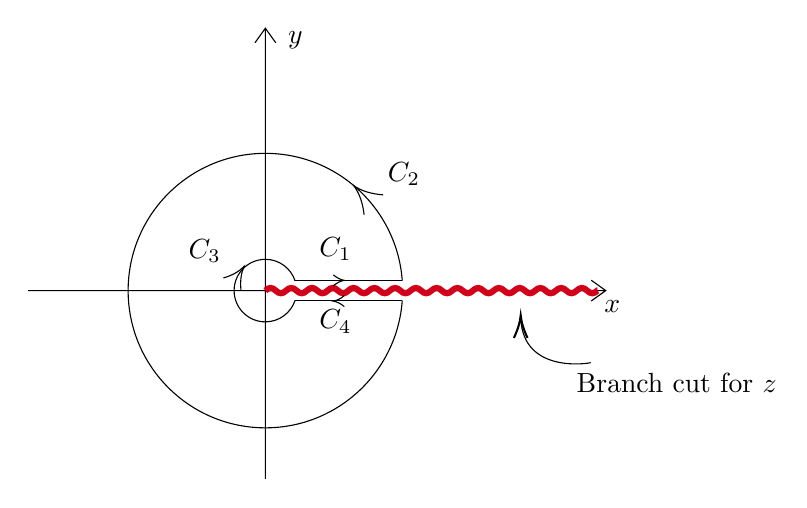
\begin{tikzpicture}[x=0.75pt,y=0.75pt,yscale=-1,xscale=1]
		%uncomment if require: \path (0,300); %set diagram left start at 0, and has height of 300
		
		%Shape: Axis 2D [id:dp6776791042565199] 
		\draw  (169,171.99) -- (447.25,171.99)(283.25,45.58) -- (283.25,262.68) (440.25,166.99) -- (447.25,171.99) -- (440.25,176.99) (278.25,52.58) -- (283.25,45.58) -- (288.25,52.58)  ;
		%Shape: Arc [id:dp4430498899507421] 
		\draw  [draw opacity=0] (349.2,176.78) .. controls (346.75,211.06) and (318.16,238.11) .. (283.25,238.11) .. controls (246.73,238.11) and (217.13,208.51) .. (217.13,171.99) .. controls (217.13,135.47) and (246.73,105.86) .. (283.25,105.86) .. controls (318.16,105.86) and (346.75,132.91) .. (349.2,167.2) -- (283.25,171.99) -- cycle ; \draw   (349.2,176.78) .. controls (346.75,211.06) and (318.16,238.11) .. (283.25,238.11) .. controls (246.73,238.11) and (217.13,208.51) .. (217.13,171.99) .. controls (217.13,135.47) and (246.73,105.86) .. (283.25,105.86) .. controls (318.16,105.86) and (346.75,132.91) .. (349.2,167.2) ;
		%Straight Lines [id:da18489737799567563] 
		\draw    (349.16,167.29) -- (297.57,167.29) ;
		%Shape: Arc [id:dp9413080197314644] 
		\draw  [draw opacity=0] (297.56,176.71) .. controls (295.57,182.72) and (289.92,187.05) .. (283.25,187.05) .. controls (274.93,187.05) and (268.19,180.3) .. (268.19,171.99) .. controls (268.19,163.67) and (274.93,156.92) .. (283.25,156.92) .. controls (289.93,156.92) and (295.6,161.27) .. (297.57,167.29) -- (283.25,171.99) -- cycle ; \draw   (297.56,176.71) .. controls (295.57,182.72) and (289.92,187.05) .. (283.25,187.05) .. controls (274.93,187.05) and (268.19,180.3) .. (268.19,171.99) .. controls (268.19,163.67) and (274.93,156.92) .. (283.25,156.92) .. controls (289.93,156.92) and (295.6,161.27) .. (297.57,167.29) ;
		%Straight Lines [id:da8886754763794343] 
		\draw    (297.56,176.71) -- (349.25,176.71) ;
		%Straight Lines [id:da13785399934572562] 
		\draw [color={rgb, 255:red, 208; green, 2; blue, 27 }  ,draw opacity=1 ][line width=2.25]    (283.25,171.99) .. controls (284.92,170.32) and (286.58,170.32) .. (288.25,171.99) .. controls (289.92,173.66) and (291.58,173.66) .. (293.25,171.99) .. controls (294.92,170.32) and (296.58,170.32) .. (298.25,171.99) .. controls (299.92,173.66) and (301.58,173.66) .. (303.25,171.99) .. controls (304.92,170.32) and (306.58,170.32) .. (308.25,171.99) .. controls (309.92,173.66) and (311.58,173.66) .. (313.25,171.99) .. controls (314.92,170.32) and (316.58,170.32) .. (318.25,171.99) .. controls (319.92,173.66) and (321.58,173.66) .. (323.25,171.99) .. controls (324.92,170.32) and (326.58,170.32) .. (328.25,171.99) .. controls (329.92,173.66) and (331.58,173.66) .. (333.25,171.99) .. controls (334.92,170.32) and (336.58,170.32) .. (338.25,171.99) .. controls (339.92,173.66) and (341.58,173.66) .. (343.25,171.99) .. controls (344.92,170.32) and (346.58,170.32) .. (348.25,171.99) .. controls (349.92,173.66) and (351.58,173.66) .. (353.25,171.99) .. controls (354.92,170.32) and (356.58,170.32) .. (358.25,171.99) .. controls (359.92,173.66) and (361.58,173.66) .. (363.25,171.99) .. controls (364.92,170.32) and (366.58,170.32) .. (368.25,171.99) .. controls (369.92,173.66) and (371.58,173.66) .. (373.25,171.99) .. controls (374.92,170.32) and (376.58,170.32) .. (378.25,171.99) .. controls (379.92,173.66) and (381.58,173.66) .. (383.25,171.99) .. controls (384.92,170.32) and (386.58,170.32) .. (388.25,171.99) .. controls (389.92,173.66) and (391.58,173.66) .. (393.25,171.99) .. controls (394.92,170.32) and (396.58,170.32) .. (398.25,171.99) .. controls (399.92,173.66) and (401.58,173.66) .. (403.25,171.99) .. controls (404.92,170.32) and (406.58,170.32) .. (408.25,171.99) .. controls (409.92,173.66) and (411.58,173.66) .. (413.25,171.99) .. controls (414.92,170.32) and (416.58,170.32) .. (418.25,171.99) .. controls (419.92,173.66) and (421.58,173.66) .. (423.25,171.99) .. controls (424.92,170.32) and (426.58,170.32) .. (428.25,171.99) .. controls (429.92,173.66) and (431.58,173.66) .. (433.25,171.99) .. controls (434.92,170.32) and (436.58,170.32) .. (438.25,171.99) .. controls (439.92,173.66) and (441.58,173.66) .. (443.25,171.99) -- (443.27,171.99) -- (443.27,171.99) ;
		\draw   (330.83,135.43) .. controls (330.19,129.71) and (328.53,125.06) .. (325.85,121.46) .. controls (329.55,123.99) and (334.27,125.45) .. (340.01,125.85) ;
		\draw   (316,164.42) .. controls (317.76,165.88) and (319.51,166.76) .. (321.27,167.05) .. controls (319.51,167.34) and (317.76,168.22) .. (316,169.68) ;
		\draw   (321.27,179.68) .. controls (319.51,178.22) and (317.76,177.34) .. (316,177.05) .. controls (317.76,176.76) and (319.51,175.88) .. (321.27,174.42) ;
		\draw   (263,165.9) .. controls (267.28,164.68) and (270.62,162.82) .. (273.02,160.31) .. controls (271.57,163.46) and (271.05,167.25) .. (271.49,171.68) ;
		%Curve Lines [id:da04977533800445433] 
		\draw    (440,206.68) .. controls (440.26,206.88) and (407.61,212.65) .. (406.31,185.58) ;
		\draw [shift={(406.27,183.88)}, rotate = 450] [color={rgb, 255:red, 0; green, 0; blue, 0 }  ][line width=0.75]    (10.93,-3.29) .. controls (6.95,-1.4) and (3.31,-0.3) .. (0,0) .. controls (3.31,0.3) and (6.95,1.4) .. (10.93,3.29)   ;
		
		% Text Node
		\draw (293,46.08) node [anchor=north west][inner sep=0.75pt]    {$y$};
		% Text Node
		\draw (445.27,175.39) node [anchor=north west][inner sep=0.75pt]    {$x$};
		% Text Node
		\draw (308,145.08) node [anchor=north west][inner sep=0.75pt]    {$C_{1}$};
		% Text Node
		\draw (341,109.08) node [anchor=north west][inner sep=0.75pt]    {$C_{2}$};
		% Text Node
		\draw (308,180.08) node [anchor=north west][inner sep=0.75pt]    {$C_{4}$};
		% Text Node
		\draw (245,146.08) node [anchor=north west][inner sep=0.75pt]    {$C_{3}$};
		% Text Node
		\draw (432,210.68) node [anchor=north west][inner sep=0.75pt]   [align=left] {Branch cut for $\displaystyle z$};
		
		
		\end{tikzpicture}
		
	\end{center}
	Then we have 
	\begin{equation*}
	\int_{C_1+C_2+C_3+C_4}\frac{z^{-x}}{1+z}\mathrm{d}z=2\uppi\mathrm{i}\;\text{Res}\;f(-1)
	\end{equation*}
	It's obviously that the integral on $C_4$ and $C_2$ is zero, thus 
	\begin{equation*}
	\int_{C_1+C_3}f\mathrm{d}z=\int_0^\infty\frac{z^{-x}}{1+z}(1-\mathrm{e}^{-2\uppi\mathrm{i}x})\mathrm{d}z=2\uppi\mathrm{i}\cdot\mathrm{e}^{-\mathrm{i}\uppi x}
	\end{equation*}
	Therefore, 
	\begin{equation*}
	\Gamma(x)\Gamma(1-x)=2\uppi\mathrm{i}\frac{\mathrm{e}^{-\uppi\mathrm{i} x}}{1-\mathrm{e}^{-2\uppi\mathrm{i}x}}=\frac{\uppi}{\sin\uppi x}
	\end{equation*}
	\subsubsection*{6.32.6}
	\begin{equation*}
	\text{Res}\;\Gamma(0)=\lim_{z\to 0}z\Gamma(z)=\lim_{z\to 0}\Gamma(z+1)=1
	\end{equation*}
	Using 
	\begin{equation*}
	\Gamma(-n)=\frac{\Gamma(-n+1)}{-n}=\cdots=\frac{(-1)^n\Gamma(0)}{n!}\;\;\Rightarrow\;\;\text{Res}\;\Gamma(-n)=\frac{(-1)^n}{n!}
	\end{equation*}
	\subsubsection*{6.32.7}
	\begin{equation*}
	\begin{split}
	\Gamma(z+1)&=\int_0^\infty\mathrm{d}t\;\mathrm{e}^{-t}t^z=\int_0^\infty\mathrm{d}t\;\mathrm{e}^{-t+z\ln t}\\
	&\simeq\int_0^\infty\mathrm{d}t\;\exp\left[-z+z\ln z-\frac 1{2z}(t-z)^2\right]\\
	&\simeq\int_{-\infty}^\infty\mathrm{d}t\;\exp\left[-z+z\ln z-\frac 1{2z}(t-z)^2\right]\\
	&=\sqrt{2\uppi z}z^z\mathrm{e}^{-z}
	\end{split}
	\end{equation*}
	and similarly, 
	\begin{equation*}
	\Gamma(ax+b)\simeq\sqrt{2\uppi}(ax+b-1)^{ax+b-1/2}\mathrm{e}^{-(ax+b)+1}\simeq\sqrt{2\uppi}\mathrm{e}^{-ax}(ax)^{ax+b-1/2}
	\end{equation*}
	\subsubsection*{6.32.8}
	Consider the path: 
		\begin{center}
			
			
			\tikzset{every picture/.style={line width=0.75pt}} %set default line width to 0.75pt        
			
			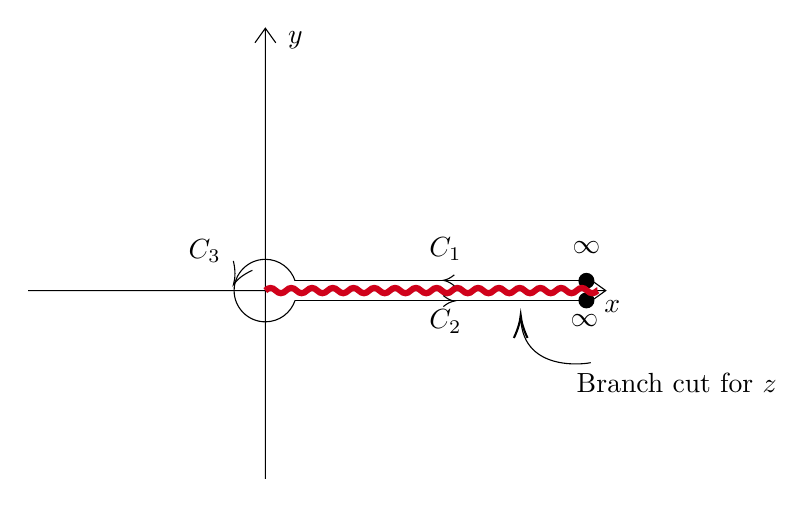
\begin{tikzpicture}[x=0.75pt,y=0.75pt,yscale=-1,xscale=1]
			%uncomment if require: \path (0,300); %set diagram left start at 0, and has height of 300
			
			%Shape: Axis 2D [id:dp6767495760239246] 
			\draw  (151,166.3) -- (429.25,166.3)(265.25,39.9) -- (265.25,257) (422.25,161.3) -- (429.25,166.3) -- (422.25,171.3) (260.25,46.9) -- (265.25,39.9) -- (270.25,46.9)  ;
			%Straight Lines [id:da07524405374351639] 
			\draw    (419.93,161.61) -- (279.57,161.61) ;
			\draw [shift={(419.93,161.61)}, rotate = 180] [color={rgb, 255:red, 0; green, 0; blue, 0 }  ][fill={rgb, 255:red, 0; green, 0; blue, 0 }  ][line width=0.75]      (0, 0) circle [x radius= 3.35, y radius= 3.35]   ;
			%Shape: Arc [id:dp06393673654396737] 
			\draw  [draw opacity=0] (279.56,171.03) .. controls (277.57,177.03) and (271.92,181.36) .. (265.25,181.36) .. controls (256.93,181.36) and (250.19,174.62) .. (250.19,166.3) .. controls (250.19,157.98) and (256.93,151.24) .. (265.25,151.24) .. controls (271.93,151.24) and (277.6,155.59) .. (279.57,161.61) -- (265.25,166.3) -- cycle ; \draw   (279.56,171.03) .. controls (277.57,177.03) and (271.92,181.36) .. (265.25,181.36) .. controls (256.93,181.36) and (250.19,174.62) .. (250.19,166.3) .. controls (250.19,157.98) and (256.93,151.24) .. (265.25,151.24) .. controls (271.93,151.24) and (277.6,155.59) .. (279.57,161.61) ;
			%Straight Lines [id:da11431230324492192] 
			\draw    (279.56,171.03) -- (419.93,171.03) ;
			\draw [shift={(419.93,171.03)}, rotate = 0] [color={rgb, 255:red, 0; green, 0; blue, 0 }  ][fill={rgb, 255:red, 0; green, 0; blue, 0 }  ][line width=0.75]      (0, 0) circle [x radius= 3.35, y radius= 3.35]   ;
			%Straight Lines [id:da8329231118245396] 
			\draw [color={rgb, 255:red, 208; green, 2; blue, 27 }  ,draw opacity=1 ][line width=2.25]    (265.25,166.3) .. controls (266.92,164.63) and (268.58,164.63) .. (270.25,166.3) .. controls (271.92,167.97) and (273.58,167.97) .. (275.25,166.3) .. controls (276.92,164.63) and (278.58,164.63) .. (280.25,166.3) .. controls (281.92,167.97) and (283.58,167.97) .. (285.25,166.3) .. controls (286.92,164.63) and (288.58,164.63) .. (290.25,166.3) .. controls (291.92,167.97) and (293.58,167.97) .. (295.25,166.3) .. controls (296.92,164.63) and (298.58,164.63) .. (300.25,166.3) .. controls (301.92,167.97) and (303.58,167.97) .. (305.25,166.3) .. controls (306.92,164.63) and (308.58,164.63) .. (310.25,166.3) .. controls (311.92,167.97) and (313.58,167.97) .. (315.25,166.3) .. controls (316.92,164.63) and (318.58,164.63) .. (320.25,166.3) .. controls (321.92,167.97) and (323.58,167.97) .. (325.25,166.3) .. controls (326.92,164.63) and (328.58,164.63) .. (330.25,166.3) .. controls (331.92,167.97) and (333.58,167.97) .. (335.25,166.3) .. controls (336.92,164.63) and (338.58,164.63) .. (340.25,166.3) .. controls (341.92,167.97) and (343.58,167.97) .. (345.25,166.3) .. controls (346.92,164.63) and (348.58,164.63) .. (350.25,166.3) .. controls (351.92,167.97) and (353.58,167.97) .. (355.25,166.3) .. controls (356.92,164.63) and (358.58,164.63) .. (360.25,166.3) .. controls (361.92,167.97) and (363.58,167.97) .. (365.25,166.3) .. controls (366.92,164.63) and (368.58,164.63) .. (370.25,166.3) .. controls (371.92,167.97) and (373.58,167.97) .. (375.25,166.3) .. controls (376.92,164.63) and (378.58,164.63) .. (380.25,166.3) .. controls (381.92,167.97) and (383.58,167.97) .. (385.25,166.3) .. controls (386.92,164.63) and (388.58,164.63) .. (390.25,166.3) .. controls (391.92,167.97) and (393.58,167.97) .. (395.25,166.3) .. controls (396.92,164.63) and (398.58,164.63) .. (400.25,166.3) .. controls (401.92,167.97) and (403.58,167.97) .. (405.25,166.3) .. controls (406.92,164.63) and (408.58,164.63) .. (410.25,166.3) .. controls (411.92,167.97) and (413.58,167.97) .. (415.25,166.3) .. controls (416.92,164.63) and (418.58,164.63) .. (420.25,166.3) .. controls (421.92,167.97) and (423.58,167.97) .. (425.25,166.3) -- (425.27,166.3) -- (425.27,166.3) ;
			\draw   (356.27,164) .. controls (354.51,162.53) and (352.76,161.66) .. (351,161.37) .. controls (352.76,161.07) and (354.51,160.19) .. (356.27,158.73) ;
			\draw   (351,168.73) .. controls (352.76,170.2) and (354.51,171.07) .. (356.27,171.37) .. controls (354.51,171.66) and (352.76,172.54) .. (351,174) ;
			\draw   (259.01,156.54) .. controls (254.93,158.34) and (251.89,160.65) .. (249.86,163.47) .. controls (250.86,160.14) and (250.85,156.32) .. (249.81,151.99) ;
			%Curve Lines [id:da4387767149446593] 
			\draw    (422,201) .. controls (422.26,201.2) and (389.61,206.96) .. (388.31,179.9) ;
			\draw [shift={(388.27,178.2)}, rotate = 450] [color={rgb, 255:red, 0; green, 0; blue, 0 }  ][line width=0.75]    (10.93,-3.29) .. controls (6.95,-1.4) and (3.31,-0.3) .. (0,0) .. controls (3.31,0.3) and (6.95,1.4) .. (10.93,3.29)   ;
			
			% Text Node
			\draw (275,40.4) node [anchor=north west][inner sep=0.75pt]    {$y$};
			% Text Node
			\draw (427.27,169.7) node [anchor=north west][inner sep=0.75pt]    {$x$};
			% Text Node
			\draw (343,139.4) node [anchor=north west][inner sep=0.75pt]    {$C_{1}$};
			% Text Node
			\draw (343,174.4) node [anchor=north west][inner sep=0.75pt]    {$C_{2}$};
			% Text Node
			\draw (227,140.4) node [anchor=north west][inner sep=0.75pt]    {$C_{3}$};
			% Text Node
			\draw (414,205) node [anchor=north west][inner sep=0.75pt]   [align=left] {Branch cut for $\displaystyle z$};
			% Text Node
			\draw (412,141.4) node [anchor=north west][inner sep=0.75pt]    {$\infty $};
			% Text Node
			\draw (411,176.4) node [anchor=north west][inner sep=0.75pt]    {$\infty $};
			
			
			\end{tikzpicture}
			
		\end{center}
	\begin{equation*}
	\Gamma(z)=\int_0^\infty\mathrm{d}t\;\mathrm{e}^{-t}t^{z-1}=-\int_{C_1}\mathrm{d}t\;\mathrm{e}^{-t}t^{z-1}
	\end{equation*}
	Noting that 
	\begin{equation*}
	\int_{C_1+C_2+C_3}\mathrm{d}t\;\mathrm{e}^{-t}t^{z-1}=-\left(1-\mathrm{e}^{2\uppi \mathrm{i}(z-1)}\right)\Gamma(z)
	\end{equation*}
	and using $\mathrm{e}^{2\uppi \mathrm{i}(z-1)}=\mathrm{e}^{2\uppi \mathrm{i}z}$ we have 
	\begin{equation*}
	\Gamma(z)=\frac{1}{\mathrm{e}^{2\uppi \mathrm{i}z}-1}\oint s^{z-1}\mathrm{e}^{-s}\mathrm{d}s
	\end{equation*}
			
	\subsection{Exercise 6.33}	
		\subsubsection*{(1)}
		Consider: 
			\begin{equation*}
			\begin{aligned}
				I=\lim_{\eta\to+ 0}\ointctrclockwise_{C_R}\frac{\me^{\omega\eta
				}}{(\me^{\beta\omega}-1)(\omega-x)}
			\end{aligned}
			\end{equation*}
			
		Has the poles: $z=\omega_{n}=\mi \frac{2\pi n}{\beta}$ and $z=x$. 
		
		Then: 
			\begin{equation*}
			\begin{aligned}
				I=2\pi \mi \left(\sum_{n}\operatorname{Res}(\omega_{n})+\operatorname{Res}(x)\right)=2 \pi \mi \cdot\left[\left(\sum_{n} \frac{1}{\beta} \frac{\me^{\mi \omega_{n} \eta}}{\mi \omega_{n}-x}\right)+\frac{\me^{\eta x}}{\me^{\beta x}-1}\right]
			\end{aligned}
			\end{equation*}
			
		As $\omega\to \infty$, we have:
			\begin{equation*}
			\begin{aligned}
				\frac{\omega}{(\me^{\beta\omega})(\omega-x)}\to 0
			\end{aligned}
			\end{equation*}
			
		Like what we did in the note, we have:
			\begin{equation*}
			\begin{aligned}
				\left|\int_{C_{R \rightarrow \infty}} f(z) \mathrm{d} z\right|=\left|\int_{C_{R \rightarrow \infty}} z f(z) \frac{\mathrm{d} z}{z}\right| &\leq \int_{C_{R \rightarrow \infty}}|z f(z)| \frac{|\mathrm{d} z|}{|z|} \leq \lim _{R \rightarrow \infty} \max |z f(z)| \pi=0\\
				\Rightarrow &I\to 0
			\end{aligned}
			\end{equation*}
			
		So our sum looks like:
			\begin{equation*}
			\begin{aligned}
				\Rightarrow \frac{1}{\beta} \lim _{\eta \rightarrow 0} \sum_{\omega_{n}} \frac{\me^{\mi \omega_{n} \eta}}{x-\mi \omega_{n}}=\lim _{\eta \rightarrow 0} \frac{\me^{\eta x}}{\me^{\beta x}-1}=\frac{1}{\me^{\beta x}-1}
			\end{aligned}
			\end{equation*}
			
		\subsubsection*{(2)}
			Consider the integration:
				\begin{equation*}
				\begin{aligned}
					\ointctrclockwise_{C_R}\frac{1}{(\omega^2-\omega_0^2)(\me^{\beta\omega}-1)}=2\pi \mi[\underbrace{\operatorname{Res}f(\omega_0)}_{\frac{1}{2\omega_0}\frac{1}{\me^{\beta\omega_0}-1}}+\underbrace{\operatorname{Res}f(-\omega_0)}_{-\frac{1}{2\omega_0}\frac{1}{\me^{-\beta\omega_0}-1}}+\underbrace{\sum_{n}\operatorname{Res}f(\mi \omega_{n})}_{-\sum_{n}\frac{1}{\beta}\frac{1}{\omega_0^2+\omega_{n}^2}}]=0
				\end{aligned}
				\end{equation*}
				
			So we have
				\begin{equation*}
				\begin{aligned}
					\sum_{n}\frac{1}{\beta}\frac{1}{\omega_0^2+\omega_{n}^2}=\frac{1}{2\omega_0}\coth\left(\frac{\beta\omega_0}{2}\right)
				\end{aligned}
				\end{equation*}
				
	\subsection{Exercise 6.34}
		\subsubsection*{(1)}
			It has the poles $z=j$.
			
			Compute directly:
			\begin{equation*}
			\begin{aligned}
			I=\frac{1}{2\mi}\ointctrclockwise_{C_R}\frac{x^t}{\Gamma^3(t+1)}\cot(\pi x)\di t=\frac{1}{2\mi}2\pi \mi \sum_{j=0}^{n-1}\operatorname{Res}f(j)=2\pi\mi \sum_{j=0}^{n-1}\lim_{t\to j}\frac{x^t}{\Gamma^3(t+1)}\frac{\cos(\pi t)}{\sin (\pi t)}(t-j)=\sum_{j=0}^{n-1}\frac{x^j}{(j!)^3}
			\end{aligned}
			\end{equation*}
%		\subsubsection*{(2)}
%			Using the hint:
%				\begin{equation*}
%				\begin{aligned}
%					\frac{\cot(\pi t)}{2\mi}=\frac{\cos(\pi t)}{2\mi \sin(\pi t)}
%				\end{aligned}
%				\end{equation*}


\section{Group Representations: Finite Groups}
\subsection{Exercise 7.1}
We need to show 
\begin{equation*}
\rho_1^{-1}(g)M(g)+\rho^{-1}(g)C\rho_2(g)=C,\;\;\forall\;g\in G
\end{equation*}
We have 
\begin{equation*}
C=a\sum_{h\in G}M(h^{-1})\rho_2(h)
\end{equation*}
Then 
\begin{align*}
&\rho_1^{-1}M(g)+\rho_1^{-1}(g)a\sum_{h\in G}M(h^{-1})\rho_2(h)\rho_2(g)\\
={}&\rho_1(g^{-1})M(g)+a\sum_{h\in G}\big[M(g^{-1}h^{-1})-M(g^{-1})\rho_2(h^{-1})\big]\rho_2(hg)\\
={}&\rho_1(g^{-1})M(g)+a\sum_{h\in G}M(g^{-1}h^{-1})\rho_2(hg)-a\sum_{h\in G}M(g^{-1})\rho_2(g)\\
={}&\rho_1(g^{-1})M(g)-a|G|M(g^{-1})\rho_2(g)+C
\end{align*}
Set 
\begin{equation*}
a=-\frac{1}{|G|}\;\;\Rightarrow\;\;\text{LHS}=\rho_1(g^{-1})M(g)+M(g^{-1})\rho_2(g)+C=M(e)+C
\end{equation*}
Thus 
\begin{equation*}
\rho(e)=\begin{pmatrix}
1 & M(e)\\ 0& 1
\end{pmatrix}\;\;\Rightarrow\;\;\rho(ee)=\begin{pmatrix}
1 & 2M(e)\\ 0 & 1
\end{pmatrix}\;\;\Rightarrow\;\;M(e)=0
\end{equation*}
Hence $\text{LHS}=\text{RHS}$. $\square$

\paragraph*{Remark} Here we take $a=-1/|G|$, so the proof is only valid for finite groups. 

\subsection{Exercise 7.2}
No. Suppose $g\in[a]$ and $g\in [b]$ with $[a]\ne [b]$. Then there exists $h\in G$ s.t. $a=h^{-1}gh$ and $h'\in G$ s.t. $b=h'^{-1}gh'$. 
Then we have 
\begin{equation*}
g=h'bh'^{-1}\;\;\Rightarrow\;\;a=h^{-1}gh=h^{-1}h'bh'^{-1}h=(h'^{-1}h)^{-1}b(h'^{-1}h)
\end{equation*}
and hence $[a]=[b]$, which is cotradict with our assumption. $\square$

\subsection{Exercise 7.3}
First we prove that $Z_g=\{h\in G|hg=gh\}$ forms a group. If $h_1,h_2\in Z_g$, then 
\begin{equation*}
(h_1h_2)g=h_1(h_2g)=h_1(gh_2)=(h_1g)h_2=(gh_1)h_2=g(h_1h_2)\;\;\Rightarrow\;\;h_1h_2\in G
\end{equation*}
If $h_1\in Z_g$, then 
\begin{equation*}
h_1^{-1}g=h_1^{-1}(gh_1)h_1^{-1}=h_1^{-1}(h_1g)h_1^{-1}=gh_1^{-1}\;\;\Rightarrow\;\;h_1^{-1}\in Z_g
\end{equation*}
Obviously $eg=g=ge$ hence $e\in Z_g$. Hence $Z_g$ forms a group. 

Second, we prove that if $g\sim g'$, then $Z_g\cong Z_{g'}$. If we have $g'=f^{-1}gf\;\Rightarrow\;fg'=gf$, then for $h\in Z_g$, we have $hfg'=hgf=ghf=fg'f^{-1}hf\;\Rightarrow\;(f^{-1}hf)g'=g'(f^{-1}hf)$. Therefore, for $h\in Z_g$, 
we have $f^{-1}hf\in Z_{f^{-1}gf}$. As $(f^{-1}h'f)(f^{-1}hf)=f^{-1}(h'h)f$, this gives a homomorphism between $Z_g$ and $Z_{g'}$. Moreover, it is an
injection because if $f^{-1}hf=f^{-1}h'f$, we have $hf=h'f$ and hence $h=h'$, and it is a surjection, because for $\forall\;h\in Z_{g'}$, we have $h'=fhf^{-1}\in Z_{g}$ s.t. $f^{-1}h'f=h$. 
Hence $Z_g\cong Z_{g'}$. $\square$ 

\subsection{Exercise 7.4}
Using the multiplication rule, we can find the conjugacy classes of $S_3$. The identity element $e$ must be a conjugacy class itself $C^1=\{e\}$. Now consider 
the cycle $(12)$. Using the multiplication table \eqref{multi-S3}, we have 
\begin{align*}
&(23)^{-1}(12)(23)=(23)(12)(23)=(132)(23)=(13)\\
&(13)^{-1}(12)(13)=(13)(12)(13)=(123)(13)=(23)\\
&(123)^{-1}(12)(123)=(132)(12)(123)=(23)(123)=(13)\\
&(132)^{-1}(12)(132)=(123)(12)(132)=(13)(132)=(23)
\end{align*}
Therefore, three 2-cycle is another conjugacy class $C^2=\{(12),(23),(13)\}$. The rest one is obviously $C^3=\{(123),(132)\}$. 

\subsection{Exercise 7.5}
\subsubsection*{7.5.1}
\begin{equation*}
\text{The number of $k$-cycles in $S_n$}=\begin{pmatrix}
k\\n
\end{pmatrix}\times k!\times\frac{1}{k}=\frac{n!}{k(n-k)!}
\end{equation*}
\subsubsection*{7.5.2}
\begin{equation*}
(a_1\cdots a_k)^{-1}=(a_ka_{k-1}\cdots a_1)
\end{equation*}
\subsubsection*{7.5.3}
\begin{equation*}
(a_1\cdots a_k)^k=\begin{pmatrix}
a_1 & a_2 & \cdots & a_k\\
a_2 & a_3 & \cdots & a_1\\
a_3 & a_4 & \cdots & a_2\\
\vdots & \vdots & \; & \vdots\\
a_1 & a_2 & \cdots & a_k
\end{pmatrix}=e
\end{equation*}
\subsubsection*{7.5.4}
\begin{equation*}
(a_1\cdots a_m)(a_1'\cdots a'_n)=\begin{pmatrix}
1 & \cdots & a_1 &\cdots& a_1'&\cdots & a_m&\cdots & a_m'\\
1 & \cdots & a_2 &\cdots &a_2'&\cdots & a_1&\cdots & a_1'
\end{pmatrix}=(a_1'\cdots a_n')(a_1\cdots a_m)
\end{equation*}
\subsubsection*{7.5.5}
We have 
\begin{equation*}
(mn)=\begin{pmatrix}
1 & \cdots & m & \cdots & n\\
1 & \cdots & n & \cdots & m
\end{pmatrix}=\begin{pmatrix}
1 & \cdots & m & \cdots & n \\
m & \cdots  &1 & \cdots & n\\
n & \cdots &1 & \cdots & m\\
1 & \cdots & n & \cdots &m
\end{pmatrix}=(1m)(1n)(1m)
\end{equation*}
\subsubsection*{7.5.6}
\paragraph*{Claim:} Any permutations in $S_n$ can be written uniquely as a product of disjoint cycles. 

\textit{Proof:} $\forall\;\sigma\in S_n, a\in A=\{1,\cdots,n\}$, 
consider $\sigma(a),\sigma^2(a),\cdots,\sigma^{m_a}(a)=a$, with $m_a$ the smallest integer s.t. $\sigma^{m_a}(a)=a$.
\paragraph*{Lemma 1} $\forall\;0\le i<j\le m_a-1$, $\sigma^i(a)\ne\sigma^j(a)$. This is because if $\sigma^i(a)=\sigma^j(a)$, then $a=\sigma^{j-i}(a)$ 
with $j-i<m_a$, which is contradict with our assumption. 

$\;$

If $m_a=n$, then $\sigma$ is an $n$-cycle and we finish the proof. If $m_a<n$, then denote $B=A\setminus\{a,\sigma(a),\cdots,\sigma^{m_a-1}(a)\}$ 
and we can choose $\forall\;b\in B$ and repeat the same procedure. 
\paragraph*{Lemma 2} $\forall\;n\in\mathbb Z^+$, $\sigma^n(b)\in B$, i.e. $\sigma^n(b)\notin\{a,\sigma(a),\cdots,\sigma^{m_a-1}(a)\}$. This is because 
if $\exists\;m$ s.t. $\sigma^n(b)=\sigma^m(a)$, then $b=\sigma^{m-n}(a)\;\;\Rightarrow\;\;b\in \{a,\sigma(a),\cdots,\sigma^{m_a-1}(a)\}$, which is 
contradict with our assumption. 

$\;$

Therefore, $\{a,\sigma(a),\cdots,\sigma^{m_a-1}(a)\}$ and $\{b,\sigma(b),\cdots,\sigma^{m_b-1}(b)\}$ are disjoint. Hence, we can repeat the 
process until we complete the proof. And Clearly we have $\sum_{j=1}^n jm_j=n$. 
\subsubsection*{7.5.7} Cycle structures of $S_4$: $C^1=[e]=[(1)(2)(3)(4)]$, $C^2=[(12)(3)(4)]$, $C^3=[(12)(34)]$, $C^4=[(123)(4)]$, $C^5=[(1234)]$. 
Consider a given partition of $n$, say $\{\lambda_i\}$ with $\sum_i\lambda_i=n$ and $\lambda_1\ge\cdots\ge\lambda_n$. 
If we let $m_j=\lambda_j-\lambda_{j+1}$, then 
\begin{equation*}
\lambda_j=\sum_{k=j}^n m_j\;\;\Rightarrow\;\;\sum_{j=1}^n jm_j=\sum_{j=1}^n\lambda_i=n
\end{equation*}
which means $\{m_j\}$ gives a cycle structure. Hence the number of cycle structures of $S_N=P(N)=n_C$. 
\subsubsection*{7.5.8}
\begin{equation*}
\text{The number of elements in cycle structure}\;\{m_j\}=\frac{n!}{\prod_jj^{m_j}m_j!}
\end{equation*}
\subsubsection*{7.5.9}
For given $\sigma\in S_n$, we have 
\begin{equation*}
\sigma(a_1\cdots a_k)\sigma^{-1}\sigma(a_m)=\sigma(a_{m+1}),\;\;a_m\in\{a_1,\cdots,a_k\}
\end{equation*}
Thus 
\begin{equation*}
\sigma(a_1\cdots a_k)\sigma^{-1}=(\sigma(a_1)\sigma(a_2)\cdots\sigma(a_k))
\end{equation*}
Suppose we have $\tilde{\rho}=\sigma\rho\sigma^{-1}$, $\rho=(\cdots)(\cdots)(\cdots)$, then $\tilde{\rho}=\rho(\cdots)\rho^{-1}\rho(\cdots)\rho^{-1}\cdots\rho(\cdots)\rho^{-1}$ 
has the same cycle structure with $\rho$. $\square$ 
\subsection{Exercise 7.6}
\begin{align*}
\rho^R((23))&=\begin{pmatrix}
0 & 0 & 1 & 0 & 0 & 0\\
0 & 0 & 0 & 0 & 0 & 1\\
1 & 0 & 0 & 0 & 0 & 0\\
0 & 0 & 0 & 0 & 1 & 0\\
0 & 0 & 0 & 1 & 0 & 0\\
0 & 1 & 0 & 0 & 0 & 0
\end{pmatrix},\;\;\rho^R((13))=\begin{pmatrix}
0 & 0 & 0 & 1 & 0 & 0\\
0 & 0 & 0 & 0 & 1 & 0\\
0 & 0 & 0 & 0 & 0 & 1\\
1 & 0 & 0 & 0 & 0 & 0\\
0 & 1 & 0 & 0 & 0 & 0\\
0 & 0 & 1 & 0 & 0 & 0
\end{pmatrix}\\
\rho^R((132))&=\begin{pmatrix}
0 & 0 & 0 & 0 & 0 & 1\\
0 & 0 & 1 & 0 & 0 & 0\\
0 & 0 & 0 & 1 & 0 & 0\\
0 & 1 & 0 & 0 & 0 & 0\\
1 & 0 & 0 & 0 & 0 & 0\\
0 & 0 & 0 & 0 & 1 & 0
\end{pmatrix}
\end{align*}
\subsection{Exercise 7.7}
We know that $(12)$ and $(123)$ are two generators of the group, which means we just need to find a matrix $S$ which simultaneously change $\rho^{3\otimes2}((12))$ to $\rho^{R}((12))$ and change $\rho^{3\otimes2}((123))$ to $\rho^{R}((123))$, then the same $S$ can apply to other group elements, for example, we know that:
	\begin{equation*}
	\begin{aligned}
		S\rho^{3\otimes2}((123))S^{-1}&=\rho^{R}((123))\\
		S\rho^{3\otimes2}((12))S^{-1}&=\rho^{R}((12))
	\end{aligned}
	\end{equation*}

Then:
	\begin{equation*}
	\begin{aligned}
		S\rho^{3\otimes2}((123))S^{-1}S\rho^{3\otimes2}((12))S^{-1}&=\rho^{R}((123))\rho^{R}((12))\\
		\Rightarrow S\rho^{3\otimes2}((13))S^{-1}&=\rho^{R}((13))
	\end{aligned}
	\end{equation*}
	
To change a matrix into another, we must turn the action of the tensor rep matrix on the basis into the action of the regular rep matrix on the basis. Call the basis of regular rep $\xi_i,i=1,2,...,6$, then the action of $(12)$ on the basis is:
	\begin{equation*}
	\begin{aligned}
		\xi_1\leftrightarrow \xi_2, \xi_3\leftrightarrow \xi_5,\xi_4\leftrightarrow \xi_6
	\end{aligned}
	\end{equation*}

The action of $(123)$ on the basis looks like:
	\begin{equation*}
	\begin{aligned}
		\xi_1\to \xi_5 \to \xi_6\to \xi_1, \xi_2\to \xi_4\to \xi _3\to \xi _2
	\end{aligned}
	\end{equation*}
	
Let's look at $  \rho^{3\otimes2} $, its basis can be viewed as the tensor product of $\rho^3$ and $\rho ^2$, and we can rename the basis of $\rho^3$ as follows:
	\begin{equation*}
	\begin{aligned}
		\eta_3^1=
		\begin{pmatrix}
			1\\
			0\\
			0
		\end{pmatrix},
		\eta_3^2=
		\begin{pmatrix}
			0\\
			1\\
			0
		\end{pmatrix},
		\eta_3^3=
		\begin{pmatrix}
			0\\
			0\\
			1
		\end{pmatrix}
	\end{aligned}
	\end{equation*}

We know $\rho^2$ acts on the coordinate of the three balls, so call them:
	\begin{equation*}
	\begin{aligned}
		\eta_2^1=
		\begin{pmatrix}
		\frac{\sqrt{3}}{2}\\
		\frac{1}{2}
		\end{pmatrix},
		\eta_2^2=
		\begin{pmatrix}
		-\frac{\sqrt{3}}{2}\\
		\frac{1}{2}
		\end{pmatrix},
		\eta_2^3=
		\begin{pmatrix}
		0\\
		-1
		\end{pmatrix}
	\end{aligned}
	\end{equation*}

The action of $\rho^2,\rho^3$ looks like:
	
	\begin{center}
		\tikzset{every picture/.style={line width=0.75pt}} %set default line width to 0.75pt        
		
		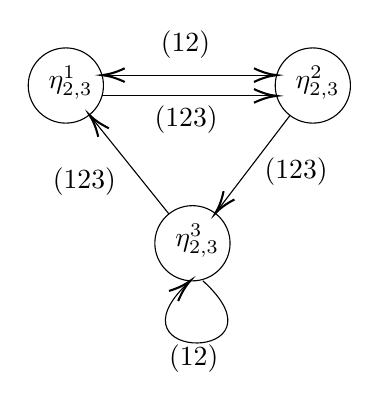
\begin{tikzpicture}[x=0.75pt,y=0.75pt,yscale=-1,xscale=1]
		%uncomment if require: \path (0,300); %set diagram left start at 0, and has height of 300
		
		%Curve Lines [id:da21357599489374146] 
		\draw    (225.5,184.05) .. controls (269.06,223.65) and (177.37,224.05) .. (218.22,185.24) ;
		\draw [shift={(219.5,184.05)}, rotate = 497.73] [color={rgb, 255:red, 0; green, 0; blue, 0 }  ][line width=0.75]    (10.93,-3.29) .. controls (6.95,-1.4) and (3.31,-0.3) .. (0,0) .. controls (3.31,0.3) and (6.95,1.4) .. (10.93,3.29)   ;
		
		% Text Node
		\draw    (159.5, 90) circle [x radius= 18.12, y radius= 18.12]   ;
		\draw (150,79.4) node [anchor=north west][inner sep=0.75pt]    {$\eta ^{1}_{2,3}$};
		% Text Node
		\draw    (220.5, 166) circle [x radius= 18.12, y radius= 18.12]   ;
		\draw (211,155.4) node [anchor=north west][inner sep=0.75pt]    {$\eta ^{3}_{2,3}$};
		% Text Node
		\draw    (278.5, 90) circle [x radius= 18.12, y radius= 18.12]   ;
		\draw (269,79.4) node [anchor=north west][inner sep=0.75pt]    {$\eta ^{2}_{2,3}$};
		% Text Node
		\draw (204,62.4) node [anchor=north west][inner sep=0.75pt]    {$( 12)$};
		% Text Node
		\draw (201,98.4) node [anchor=north west][inner sep=0.75pt]    {$( 123)$};
		% Text Node
		\draw (254,123.4) node [anchor=north west][inner sep=0.75pt]    {$( 123)$};
		% Text Node
		\draw (152,128.4) node [anchor=north west][inner sep=0.75pt]    {$( 123)$};
		% Text Node
		\draw (208,213.4) node [anchor=north west][inner sep=0.75pt]    {$( 12)$};
		% Connection
		\draw    (178.92,85) -- (259.08,85) ;
		\draw [shift={(261.08,85)}, rotate = 180] [color={rgb, 255:red, 0; green, 0; blue, 0 }  ][line width=0.75]    (10.93,-3.29) .. controls (6.95,-1.4) and (3.31,-0.3) .. (0,0) .. controls (3.31,0.3) and (6.95,1.4) .. (10.93,3.29)   ;
		\draw [shift={(176.92,85)}, rotate = 0] [color={rgb, 255:red, 0; green, 0; blue, 0 }  ][line width=0.75]    (10.93,-3.29) .. controls (6.95,-1.4) and (3.31,-0.3) .. (0,0) .. controls (3.31,0.3) and (6.95,1.4) .. (10.93,3.29)   ;
		% Connection
		\draw    (176.92,95) -- (259.08,95) ;
		\draw [shift={(261.08,95)}, rotate = 180] [color={rgb, 255:red, 0; green, 0; blue, 0 }  ][line width=0.75]    (10.93,-3.29) .. controls (6.95,-1.4) and (3.31,-0.3) .. (0,0) .. controls (3.31,0.3) and (6.95,1.4) .. (10.93,3.29)   ;
		% Connection
		\draw    (267.51,104.4) -- (232.71,150.01) ;
		\draw [shift={(231.49,151.6)}, rotate = 307.35] [color={rgb, 255:red, 0; green, 0; blue, 0 }  ][line width=0.75]    (10.93,-3.29) .. controls (6.95,-1.4) and (3.31,-0.3) .. (0,0) .. controls (3.31,0.3) and (6.95,1.4) .. (10.93,3.29)   ;
		% Connection
		\draw    (209.16,151.87) -- (172.09,105.69) ;
		\draw [shift={(170.84,104.13)}, rotate = 411.25] [color={rgb, 255:red, 0; green, 0; blue, 0 }  ][line width=0.75]    (10.93,-3.29) .. controls (6.95,-1.4) and (3.31,-0.3) .. (0,0) .. controls (3.31,0.3) and (6.95,1.4) .. (10.93,3.29)   ;
		
		\end{tikzpicture}
		
	\end{center}

Next we shall find a new tensor product basis that the action of $\rho^{3\otimes2}$ on it is exactly the same as the action of $\rho^R$. Let's call:
	\begin{equation*}
	\begin{aligned}
		\eta_1=\eta_3^1\otimes \eta_2^2
	\end{aligned}
	\end{equation*}
	
Then, what does $\eta_2$ looks like? Act $\rho^{3\otimes2}(12)$, we can get
	\begin{equation*}
	\begin{aligned}
		\eta_2=\eta_3^2\otimes \eta_2^1
	\end{aligned}
	\end{equation*}
	
According to the action of $\rho^R(123)$ on $\xi_1$, we can get:
	\begin{equation*}
	\begin{aligned}
		\eta_5=\rho^{3\otimes2}(123)\eta_1=\rho^{3\otimes2}(123)\eta_3^1\otimes \eta_2^2=\eta_3^2\otimes \eta_2^3
	\end{aligned}
	\end{equation*}
	
Similarly, if we act $\rho^{3\otimes2}(123)$ on $\eta_2$, we can get:
	\begin{equation*}
	\begin{aligned}
		\eta_4=\eta_3^3\otimes \eta_2^2
	\end{aligned}
	\end{equation*}
	
Apply the same method, we can get all six basis:
	\begin{equation*}
	\begin{aligned}
		\eta_1&=\eta_3^1\otimes \eta_2^2=
		\begin{pmatrix}
			-\frac{\sqrt{3}}{2}\\
			\frac{1}{2}\\
			0\\
			0\\
			0\\
			0
		\end{pmatrix},
		\eta_2=\eta_2^3\otimes \eta_2^1=
		\begin{pmatrix}
		0\\
		0\\
		\frac{\sqrt{3}}{2}\\
		\frac{1}{2}\\
		0\\
		0\\
		\end{pmatrix},
		\eta_3=\eta_3^1\otimes \eta_2^3=
		\begin{pmatrix}
		0\\
		-1\\
		0\\
		0\\
		0\\
		0
		\end{pmatrix}\\
		\eta_4&=\eta_3^3\otimes \eta_2^2=
		\begin{pmatrix}
			0\\
			0\\
			0\\
			0\\
			-\frac{\sqrt{3}}{2}\\
			\frac{1}{2}\\
		\end{pmatrix},
		\eta_5=\eta_3^2\otimes \eta_2^3=
		\begin{pmatrix}
		0\\
		0\\
		0\\
		-1\\
		0\\
		0
		\end{pmatrix}
		\eta_6=\eta_3^3\otimes \eta_2^1=
		\begin{pmatrix}
		0\\
		0\\
		0\\
		0\\
		\frac{\sqrt{3}}{2}\\
		\frac{1}{2}\\
		\end{pmatrix}
	\end{aligned}
	\end{equation*}
	
You can check that the action on six basis is the same as the action of $\rho^r$ on its basis. So the matrix $S$ looks like:
	\begin{equation*}
	\begin{aligned}
	S=\left(
	\begin{array}{cccccc}
	-\frac{\sqrt{3}}{2} & 0 & 0 & 0 & 0 & 0 \\
	\frac{1}{2} & 0 & -1 & 0 & 0 & 0 \\
	0 & \frac{\sqrt{3}}{2} & 0 & 0 & 0 & 0 \\
	0 & \frac{1}{2} & 0 & 0 & -1 & 0 \\
	0 & 0 & 0 & -\frac{\sqrt{3}}{2} & 0 & \frac{\sqrt{3}}{2} \\
	0 & 0 & 0 & \frac{1}{2} & 0 & \frac{1}{2} \\
	\end{array}
	\right)
	\end{aligned}
	\end{equation*}
	
\paragraph{Remark} Using this method, we can find that the regular representation of $D_n$ is similar to the tensor product of its $n$-d representation that comes from the defining rep of $S_n$ and its 2-d defining representation. 
	
\subsection{Exercise 7.8}
$A_3=\{e,(123),(132)\}\cong\mathbb Z_3$ thus $A_3$ is Abelian. Therefore, the representation $\rho^2$ must be decompose (as a representation of $A_3$) 
into 2 1-dim irreducible representation 
\begin{equation*}
\rho^2(e)=\begin{pmatrix}
1 & 0\\ 0 & 1
\end{pmatrix},\;\;\rho^2((123))=\begin{pmatrix}
-1/2 & -\sqrt{3}/2\\
\sqrt{3}/2 & -1/2
\end{pmatrix},\;\;\rho^2((132))=\begin{pmatrix}
-1/2 & \sqrt{3}/2\\
-\sqrt{3}/2 & -1/2
\end{pmatrix}
\end{equation*}
which is actually three matrix in $\text{SO}(2)$ with $\theta=0,2\pi/3$ and $4\pi/3$. Therefore, let 
\begin{equation*}
S=\frac{1}{\sqrt{2}}\begin{pmatrix}
1 & -\mathrm{i}\\
1 & +\mathrm{i}
\end{pmatrix}
\end{equation*}
Then 
\begin{equation*}
S\rho^2(e)S^{-1}=\begin{pmatrix}
1 & 0\\ 
0 & 1
\end{pmatrix},\;\;S\rho^2((123))S^{-1}=\begin{pmatrix}
\mathrm{e}^{-2\pi\mathrm{i}/3} & 0\\
0 & \mathrm{e}^{2\pi\mathrm{i}/3}
\end{pmatrix},\;\;S\rho^2((132))S^{-1}=\begin{pmatrix}
\mathrm{e}^{-4\pi\mathrm{i}/3} & 0\\
0 & \mathrm{e}^{4\pi\mathrm{i}/3}
\end{pmatrix}
\end{equation*}
\subsection{Exercise 7.9}
If $\rho:G\to\text{GL}(V)$ is irreducible, then there exists a subspace $V_1\subset V$ s.t. $\rho(g)V_1=V_1$. Then define a projector $P_1$ s.t. 
$P_1V=V_1$. Without loss of generality, we assume that $P_1$ is Hermitian. Since 
\begin{equation*}
P_1\rho(g)P_1=\rho(g)P_1\;\;\Rightarrow\;\;P_1\rho^\dagger(g)P_1=P_1\rho(g^{-1})P_1=P_1\rho^\dagger(g)=P_1\rho(g^{-1}),\;\;\forall\;g\in G
\end{equation*}
we have 
\begin{equation*}
P_1\rho(g)P_1=P_1\rho(g),\;\;\forall\;g\in G
\end{equation*}
Now define another projector $P_2=1-P_1$. Then we have $P_2\rho(g)P_2=\rho(g)P_2$, i.e., $P_2V=V_2$ is an invariant subspace under $\rho(g)$. 
This is because $(1-P_1)\rho(g)(1-P_1)=\rho(g)-P_1\rho(g)-\rho(g)P_1+P_1\rho(g)P_1=\rho(g)(1-P_1)=\rho(g)P_2$. 
Since $V_1\cap V_2=\emptyset$, we have $V=V_1\oplus V_2$, i.e., $(\rho,V)$ is fully reducible. 
\subsection{Exercise 7.10}
For $|w\rangle\in\text{im}T$, then there exists $|v\rangle\in V$ s.t. $|w\rangle=T|v\rangle$. Hence $\rho_W|w\rangle=\rho_W T|v\rangle=T(\rho_V|v\rangle)\in\text{im}T$. $\square$
\subsection{Exercise 7.11}
As $\rho$ is a square matrix, then if $\rho_1\rho_2=1$, $\rho_2\rho_1=1$. As we already know $\rho^\dagger\rho=1$, we have $\rho\rho^\dagger=1$. 
Otherwise, you can calculate 
\begin{equation*}
\rho\rho^\dagger=\sqrt{D}U\tilde{\rho}U^\dagger\sqrt{D}^{-1}\sqrt{D}^{-1}U\tilde{\rho}^\dagger U^\dagger\sqrt{D}=\left(\sqrt{D}^{-1}U\tilde{\rho}^\dagger U^\dagger\sqrt{D}\sqrt{D}U\tilde{\rho}U^\dagger\sqrt{D}^{-1}\right)^{-1}=\mathbf 1_{\text{dim}V}
\end{equation*}
\subsection{Exercise 7.12}
You can use the following python mini program to check the case where $\mu=2$ and $\nu=2$: 

$\;$

import numpy as np

p2 = np.zeros((6,2,2))

p2[0] += np.array([[1,0],[0,1]])

p2[1] += np.array([[-1,0],[0,1]])

p2[2] += np.array([[1/2,np.sqrt(3)/2],[np.sqrt(3)/2,-1/2]])

p2[3] += np.array([[1/2,-np.sqrt(3)/2],[-np.sqrt(3)/2,-1/2]])

p2[4] += np.array([[-1/2,-np.sqrt(3)/2],[np.sqrt(3)/2,-1/2]])

p2[5] += np.array([[-1/2,np.sqrt(3)/2],[-np.sqrt(3)/2,-1/2]])

ans = np.zeros((2,2,2,2))

got = np.zeros((2,2,2,2))

for a,b,k,l in zip(range(2),range(2),range(2),range(2)):

$\;\;\;\;$got[a,b,k,l] += 3*(a==k)*(b==l)

$\;\;\;\;$for g in range(6):

$\;\;\;\;\;\;\;\;$ans[a,b,k,l] += p2[g,a,b]*p2[g,k,l]

np.rint(ans)==np.rint(got)

$\;$

For the other cases, you can write similar program. 
\subsection{Exercise 7.13}
We have 
\begin{equation*}
\sum_{\mu=1}^{r}n_\mu^2=\frac{1}{|G|}\sum_{A=1}^3n_A\chi_A^{2*}\chi_A^2=\frac{1}{6}(1\cdot 2^2+3\cdot 0^2+2\cdot 1^2)=1
\end{equation*}
Therefore $2$ is irreducible. 
\subsection{Exercise 7.14}
\subsubsection*{7.14.1}
The linearity of the transformation can be seen from the next problem. 
\subsubsection*{7.14.2}
Noting that 
\begin{equation*}
X_k=\sum_{n=0}^{N-1}x_n\mathrm{e}^{-\mathrm{i}2\pi kn/N},\;\;0\le k\le N-1
\end{equation*}
we immediately have, if we let $w=\mathrm{e}^{-\mathrm{i}2\pi/N}$, then 
\begin{align*}
X&\equiv \begin{pmatrix}
X_0\\X_1\\X_2\\\vdots\\X_{N-1}
\end{pmatrix}=\begin{pmatrix}
1 & 1 & 1 & \cdots & 1\\ 
1 & w & w^2 & \cdots & w^{N-1}\\
1 & w^2 & w ^4 & \cdots & w^{2(N-1)}\\
\vdots & \vdots & \vdots & \; & \vdots\\
1 & w^{N-1} & w^{2(N-1)} & \cdots & w^{(N-1)^2}
\end{pmatrix}\begin{pmatrix}
x_0\\x_1\\x_2\\\vdots\\x_{N-1}
\end{pmatrix}\\&\equiv\begin{pmatrix}
\mathbf W_{0} & \mathbf W_{1} & \mathbf{W}_2 & \cdots & \mathbf W_{N-1}
\end{pmatrix}x
\end{align*}
Thus the transformation is linear, which can be written as $X=Wx$. Noting that $w^N=1$, we have 
\begin{equation*}
\frac{1}{N}W^\dagger W=\mathbf 1\;\;\Rightarrow\;\;W^{-1}=\frac{1}{N}W^\dagger\;\;\Rightarrow\;\;x=\frac{1}{N}W^\dagger X
\end{equation*}
which is the inverse discerte Fourier transformation. 
\subsubsection*{7.14.3}
We have 
\begin{equation*}
x_{N-n}=\frac{1}{N}\mathbf W_{N-n}^\dagger\cdot X=\frac{1}{N}\sum_{k=0}^{N-1}\big[\mathrm{e}^{-\mathrm{i}2\pi(N-n)k/N}\big]^*X_k=\frac{1}{N}\sum_{k=1}^{N-1}w^{nk}X_k
\end{equation*}
\subsubsection*{7.14.4}
If $x_n$'s are real, then $x_n=x_n^*$. Hence 
\begin{equation*}
\sum_{k=0}^{N-1}w^{-nk}X_k=\sum_{k=0}^{N-1}w^{nk}X_k^*=\sum_{k'=0}^{N-1}w^{(N-k')n}X_{N-k'}^*=\underbrace{w^{nN}}_{=1}\sum_{k=0}^{N-1}w^{-nk}X_{N-k}^*
\end{equation*}
which implies 
\begin{equation*}
\sum_{k=0}^{N-1}w^{-nk}(X_k-X_{N-k}^*)=0\;\;\Rightarrow\;\;X_k=X_{N-k}^*
\end{equation*}
\subsubsection*{7.14.5}
For $w^{kN}=1$ with $0\le k\le N-1$, we have $1+w^{k}+w^{2k}+\cdots+w^{(N-1)k}=0$ becuase 
\begin{equation*}
w^{kN}-1=(w^k-1)(1+w^{k}+w^{2k}+\cdots+w^{(N-1)k})
\end{equation*}
while $w^k\ne 0$. Noting that $w^*=w^{-1}$, we have 
\begin{align*}
\mathbf W_k^\dagger\cdot\mathbf W_{k'}&=1+w^{*k} w^{k'}+w^{*2k}w^{2k'}+\cdots +w^{*(N-1)k}w^{(N-1)k'}\\
&=1+w^{k'-k}+w^{2(k'-k)}+\cdots+w^{(N-1)(k'-k)}\\
&=N\delta_{kk'}
\end{align*}
which means $W^\dagger W=N\mathbf 1$, as we have mentioned in problem 7.14.1. 
\subsubsection*{7.14.6}
If we define the inner product as 
\begin{equation*}
\langle n|m\rangle=\frac{1}{N}\sum_{k=0}^{N-1}w^{*nk}w^{mk}=\frac{1}{N}\sum_{k=0}^{N-1}w^{(m-n)k}=\delta_{mn}
\end{equation*}
Therefore the basis $\{|m\rangle=\omega^m\}$ is orthogonal. 
\subsubsection*{7.14.7}
\begin{equation*}
x_{N+n}=\frac{1}{N}\sum_{k=0}^{N-1}w^{-(N+n)k}X_k\overset{w^N=1}{=}\frac{1}{N}\sum_{k=0}^{N-1}w^{-nk}X_k=x_n
\end{equation*}
\subsubsection*{7.14.8}
\begin{equation*}
X_{k+N}=\frac{1}{N}\sum_{n=0}^{N-1}w^{n(k+N)}x_n\overset{w^N=1}{=}\sum_{n=0}^{N-1}w^{nk}x_n=X_k
\end{equation*}
\subsubsection*{7.14.9}
Shift theorem: if we shift $x_n\mapsto \mathrm{e}^{2\pi\mathrm{i}mn/N}x_n=w^{-mn}x_n$, we then have 
\begin{equation*}
X_k\mapsto\frac{1}{N}\sum_{n=0}^{N-1}w^{nk}w^{-mn}x_n=X_{k-m}
\end{equation*}
\subsubsection*{7.14.10}
Circular shift operator: Define $\tau_m$ s.t. $(\tau_mx)_n=x_{n-m}$, then 
\begin{equation*}
X_k(\tau_m x)=X_k(x_{n-m})=\frac{1}{N}\sum_{n=0}^{N-1}x_{n-m}w^{-nk}=w^{mk}X_k
\end{equation*}
\subsubsection*{7.14.11}
As 
\begin{equation*}
X_k=\sum_{n=0}^{N-1}w^{nk}x_n,\;\;Y_k^*=\sum_{m=0}^{N-1}w^{-mk}y_m^*
\end{equation*}
we have 
\begin{equation*}
\frac{1}{N}\sum_{k=0}^{N-1}X_kY_k^*=\sum_{n=0}^{N-1}\sum_{m=0}^{N-1}x_n y_m^*\underbrace{\frac{1}{N}\sum_{k=0}^{N-1}w^{(n-m)k}}_{\delta_{mn}}=\sum_{n=0}^{N-1}x_ny_n^*
\end{equation*}
This is the famous Parseval's theorem. 
\subsubsection*{7.14.12}
Convolution: 
\begin{equation*}
(XY)_k=\sum_{n=0}^{N-1}x_ny_n\mathrm{e}^{-2\pi\mathrm{i}kn/N}=\sum_{n=0}^{N-1}x_nz_n^*=\frac{1}{N}\sum_{k'=0}^{N-1}X_{k'}Z_{k'}^*
\end{equation*}
where 
\begin{equation*}
z_n=y_n^*\mathrm{e}^{-2\pi\mathrm{i}kn/N}=y_n^*w^{-nk}\;\;\Rightarrow\;\;Z_{k'}^*=\sum_{n=0}^{N-1}(w^{nk'}z_n)^*=\sum_{n=0}^{N-1}y_nw^{n(k-k')}=Y_{k-k'}
\end{equation*}
Therefore we have 
\begin{equation*}
(XY)_k=\frac{1}{N}\sum_{l=0}^{N-1}X_{l}Y_{k-l}^*
\end{equation*}
i.e., the DFT of the products of two signal is the convolution of their spectrum. 
\subsubsection*{7.14.13}
We have 
\begin{equation*}
x_n=\cos(12\pi\times 0.05 n)=\frac{1}{2}\left(\mathrm{e}^{3\pi\mathrm{i}n/5}+\mathrm{e}^{-3\pi\mathrm{i}/5}\right)
\end{equation*}
Then 
\begin{align*}
X_k&=\sum_{n=0}^{19}x_n\mathrm{e}^{-\mathrm{i}\pi nk/10}=\frac{1}{2}\sum_{n=0}^{19}\left(\mathrm{e}^{\mathrm{i}\left(\frac{3}{5}-\frac{k}{10}\right)\pi n}+\mathrm{e}^{-\mathrm{i}\left(\frac{3}{5}+\frac{k}{10}\right)\pi n}\right)\\
&=10\delta_{k,6}+10\delta_{k,14}
\end{align*}

\subsection{Exercise 7.15}
As 
\begin{equation*}
x_n=\begin{cases}
1 & 0\le n\le k-1\\
0 & k\le n\le N-1
\end{cases}
\end{equation*}
we have 
\begin{equation*}
X_\mu=\sum_{n=0}^{k-1}\mathrm{e}^{-\mathrm{i}2\pi n\mu /N}=\begin{cases}
\dfrac{1-\exp(-\mathrm{i}2\pi k\mu/N)}{1-\exp(-\mathrm{i}2\pi \mu/N)} & \mu\ne 0\\
k & \mu=0
\end{cases}
\end{equation*}
Using the Parseval's theorem, we have 
\begin{equation*}
\frac{1}{N}\sum_{\mu=0}^{N-1}X_\mu X_\mu^*=\frac{1}{N}\left(k^2+\sum_{\mu=1}^{N-1}\frac{2-2\cos(2\pi\mu k/N)}{2-2\cos(2\pi\mu/N)}\right)=\sum_{n=0}^{N-1}x_n x_n^*=k
\end{equation*}
Thus we have 
\begin{equation*}
\sum_{\mu=1}^{N-1}\frac{1-\cos(2\pi\mu k/N)}{1-\cos(2\pi\mu/N)}=Nk-k^2
\end{equation*}

\subsection{Exercise 7.16}
\subsubsection*{7.16.1}
\begin{align}\label{state}
&\bigotimes_{i=1}^n\left(\frac{1}{\sqrt{2}}\sum_{x_i=0}^1|x_i\rangle\right)\otimes\bigotimes_{i=n+1}^{2n}|0\rangle\notag\\
={}&\otimes^n\left(\frac{1}{\sqrt{2}}|1\rangle+\frac{1}{\sqrt{2}}|0\rangle\right)\otimes(\otimes^n|0\rangle)\notag\\
={}&\frac{1}{\sqrt{2^n}}\big(|0,0,\cdots,0\rangle+|1,0,\cdots,0\rangle+|0,1,\cdots,0\rangle+\cdots+|1,1,\cdots,1\rangle\big)\otimes(\otimes^n|0\rangle)\notag\\
={}&\frac{1}{\sqrt{Q}}\sum_{x=0}^{Q-1}|x,0\rangle
\end{align}
where $Q=2^n$. 
\subsubsection*{7.16.2}
If $N=3$, $n=3$ and $a=2$, then $f(x)=2^x(\text{mod}\;3)$, which implies that $f(0)=1$, $f(1)=2$, $f(2)=1$, i.e., $r=2$. Therefore, 
\begin{align*}
U_f&=\sum_{x=0}^{Q-1}|x,f(x)\rangle\langle x,0|\\
&=|0,1\rangle\langle 1,0|+|1,2\rangle\langle 1,0|+|2,1\rangle\langle 1,0|+|2,1\rangle\langle 2,0|+|3,2\rangle\langle3,0|\\
&\;\;+|4,1\rangle\langle 4,0|+|5,2\rangle\langle 5,0|+|6,1\rangle\langle 6,0|+|7,2\rangle\langle 7,0|
\end{align*}
\subsubsection*{7.16.3}
Apply $U_f$ to Eq.\eqref{state} we have 
\begin{equation*}
U_f\frac{1}{\sqrt{Q}}\sum_{x=0}^{Q-1}|x,0\rangle=\frac{1}{\sqrt{Q}}\sum_{x=0}^{Q-1}|x,f(x)\rangle
\end{equation*}
which is entangled. 
\subsubsection*{7.16.4}
Quantum Fourier transform: 
\begin{equation*}
U_{\text{QFT}}:|x\rangle\mapsto\frac{1}{\sqrt{Q}}\sum_{y=0}^{Q-1}w^{xy}|y\rangle,\;\;w=\exp\left(\pm\frac{2\pi\mathrm{i}}{Q}\right)
\end{equation*}
Noting that the quantum Fourier transform is unitary: 
\begin{equation*}
\langle x'|U_{\text{QFT}}^\dagger U_\text{QFT}|x\rangle=\frac{1}{Q}\sum_{y'=0}^{Q-1}\sum_{y=0}^{Q-1}\langle y'|w^{-x'y'}w^{xy}|y\rangle=\frac{1}{Q}\sum_{y=0}^{Q-1}w^{(x-x')y}=\delta_{xx'}=\langle x'|x\rangle
\end{equation*}
Then 
\begin{equation*}
U_\text{QFT}U_f\frac{1}{\sqrt{Q}}\sum_{x=0}^{Q-1}|x,0\rangle=\frac{1}{Q}\sum_{x=0}^{Q-1}\sum_{y=0}^{Q-1}w^{xy}|y,f(x)\rangle\overset{!}{=}\sum_{z=0}^{N-1}\sum_{y=0}^{Q-1}A(y,z)|y,z\rangle
\end{equation*}
Therefor we have 
\begin{equation*}
A(y,z)=\frac{1}{Q}\underset{0\le x\le Q-1}{\sum_{f(x)=z}}w^{xy}
\end{equation*}
\subsubsection*{7.16.5}
Noting that all $x$'s satisfy $f(x)=z$ and $0\le x\le Q-1$ form the following set
\begin{equation*}
\left\{x_0,x_0+r,x_0+2r,\cdots,x_0+\left\lfloor\frac{Q-1-x_0}{r}\right\rfloor r=x_0+b_\text{max} r\right\}\equiv S
\end{equation*}
Therefore 
\begin{equation*}
A(y,z)=\frac{1}{Q}\sum_{x\in S}w^{xy}=\frac{1}{Q}\sum_{b}w^{(x_0+rb)y}=\frac{1}{Q}w^{x_0y}\frac{1-w^{rb_\text{max} y}}{1-\omega^{ry}}
\end{equation*}
\subsubsection*{7.16.6}
Since $U_f$ and $U_\text{QFT}$ is unitary, the probability to obtain $|y,z\rangle$ is $|A(y,z)|^2$: 
\begin{align*}
P(y,z)&=|A(y,z)|^2=\left|\frac{1}{Q}w^{x_0y}\frac{1-w^{rb_\text{max} y}}{1-\omega^{ry}}\right|\\
&=\frac{1}{Q^2}\frac{1-\cos(2\pi rb_{\text{max}}y/Q)}{1-\cos(2\pi ry/Q)}
\end{align*}
\subsubsection*{7.16.7}
The probability of obtaining certain outcome $z$ from the last $n$ qubits is given by 
\begin{equation*}
p(z)=\sum_{y=0}^{Q-1}P(y,z)=\frac{1}{Q^2}\sum_{y=0}^{Q-1}\frac{1-\cos(2\pi rb_{\text{max}}y/Q)}{1-\cos(2\pi ry/Q)}
\end{equation*}
\subsection{Exercise 7.17}
It's suffices to prove for square matrices $A$ and $B$, $AB=1$ implies $BA=1$. In fact, 
\begin{equation*}
ABA=A\;\;\Rightarrow\;\;A(BA-1)=0\;\;\Rightarrow\;\;BA(BA-1)=0\;\;\Rightarrow\;\;BA=1
\end{equation*}
\subsection{Exercise 7.18}
we have the following character table with empty spots to be filled: 
\begin{equation*}
\begin{array}{c|ccc}
\Xhline{0.7pt}
& 1 & \bar 1 & 2 \\
\hline
[e] & 1 & 1 & 2 \\
{[(12)]} & 1 & a & b \\
{[(123)]} & 1 & c & d \\
\Xhline{0.7pt}
\end{array}
\end{equation*}
There are four unkowns $a$, $b$, $c$ and $d$ in the character table above, as well as four orthogonality conditions, which can fix the four unkowns. 
To fix $a$ and $c$, use the orthogonality between the column vectors $\chi^1$ and $\chi^{\bar 1}$, i.e., 
\begin{equation*}
1+3a+2c=0
\end{equation*}
Since $\bar 1$ is 1-dimensional, the only solution would be $a=-1$ and $c=1$. Then the orthogonalities between column vectors $\chi^1$ and $\chi^2$ and 
between $\chi^{\bar 1}$ and $\chi^2$ give 
\begin{equation*}
2+3b+2d=0,\;2+3ab+2cd=2-3b+2d=0\;\;\Rightarrow\;\;b=0,\;d=-1
\end{equation*}
Thus we complete the character table of $S_3$: 
\begin{equation*}
\begin{array}{c|c|ccc}
\Xhline{0.7pt}
& n_C & 1 & \bar 1& 2\\
\hline 
[e] & 1 & 1 & 1 & 2\\
{[(12)]} & 3 & 1 & -1 & 0\\
{[(123)]} & 2 & 1 & 1 & -1\\
\Xhline{0.7pt}
\end{array}
\end{equation*}
\subsection{Exercise 7.19}
The character table of $A_3$ is 
\begin{equation*}
\begin{array}{c|c|ccc}
\Xhline{0.7pt}
& n_C & 1 & \omega& \bar\omega\\
\hline 
[e] & 1 & 1 & 1 & 2\\
{[(123)]} & 1 & 1 & \omega & \bar\omega\\
{[(132)]} & 1 & 1 & \bar\omega & \omega\\
\Xhline{0.7pt}
\end{array}
\end{equation*}
Characters of $\bar 1$ have noting to do with $A_3$. The character table of $A_3$ can be extracted from the character table of $S_3$ by 
decomposing the 2 representation of $S_3$: 
\begin{equation*}
\rho^2=\rho^\omega\oplus\rho^{\bar\omega}
\end{equation*}
because 
\begin{equation*}
n_1=\frac{1}{|G|}\sum_{A=1}^3n_A\chi_A^{1*}\chi_A=\frac 13(2-1-1)=0,\;\;n_\omega=\frac{1}{3}(2-\bar \omega-\omega)=1=n_{\bar\omega}
\end{equation*}
\subsection{Exercise 7.20}
The young tableaux of $S_4$: 
\begin{equation*}
\begin{ytableau}
\; \\ \;\\ \;\\ \;
\end{ytableau}\;\;d_1=\frac{4!}{4!}=1,\;\;\begin{ytableau}
\; & \; \\ \; \\ \;
\end{ytableau}\;\;d_2=\frac{4!}{4\times 2}=3,\;\;\begin{ytableau}
\; & \;\\ \;& \;
\end{ytableau}\;\;d_3=\frac{4!}{3\times 2\times 1\times 2}=2
\end{equation*}
\begin{equation*}
\begin{ytableau}
\; & \; & \;\\\;
\end{ytableau}\;\;d_4=\frac{4!}{4\times 1\times 2}=3,\;\;\begin{ytableau}
\; & \; & \; & \; 
\end{ytableau}\;\;d_5=\frac{4!}{4!}=1
\end{equation*}
Thus we have $1^2+3^2+2^2+3^2+1^2=24=|S_4|$ as desired. 

The young tableaux of $S_5$: 
\begin{equation*}
\begin{ytableau}
\; \\\;\\\;\\\;\\\;
\end{ytableau}\;\;d_1=\frac{5!}{5!}=1,\;\;\begin{ytableau}
\; & \;\\\;\\\;\\\;
\end{ytableau}\;\;d_2=\frac{5!}{5\times 3\times 2}=4,\;\;\begin{ytableau}
\; & \;\\\;&\;\\\;
\end{ytableau}\;\;d_3=\frac{5!}{4\times 3\times 2}=5
\end{equation*}
\begin{equation*}
\begin{ytableau}
\; & \; & \;\\
\;\\\;
\end{ytableau}\;\;d_4=\frac{5!}{5\times 2\times 2}=6,\;\;\begin{ytableau}
\;& \; & \; & \\
\; & \;
\end{ytableau}\;\;d_5=\frac{5!}{4\times 2\times 3}=5
\end{equation*}
\begin{equation*}
\begin{ytableau}
\; & \;& \;& \;\\
\;
\end{ytableau}\;\;d_6=\frac{5!}{5\times 3\times 2}=4,\;\;\begin{ytableau}
\;&\;&\;&\;&\;
\end{ytableau}\;\;d_7=\frac{5!}{5!}=1
\end{equation*}
Thus we have $1^2+4^2+5^2+6^2+5^2+4^2+1^2=120=|S_5|$ as desired. 

The character table of $S_4$ is given by 
\begin{equation*}
\begin{array}{c|c|ccccc}
\Xhline{0.7pt}
& n_C & 1 & \bar 1& 2 & 3 & 3'\\
\hline 
[e] & 1 & 1 & 1 & 2 & 3 & 3\\
{[(12)]} & 6 & 1 & -1 & 0 & 1 & -1\\
{[(12)(34)]} & 3 & 1 & 1 & 2 & -1 & -1\\
{[(123)]} & 8 & 1 & 1 & -1 & 0 & 0\\
{[(1234)]} & 6 & 1 & -1 & 0 & -1 & 1\\
\Xhline{0.7pt}
\end{array}
\end{equation*}
where $1$ is the trivial representation, $\bar 1$ is the signature representation, $3$ is the standard representation with $1\oplus 3=\text{defining representation}$ and 
$3'=\bar 1\otimes 3$. 

The character table of $S_5$ is given by 
\begin{equation*}
\begin{array}{c|c|ccccccc}
\Xhline{0.7pt}
& n_C & 1 & \bar 1& 4 & 4' & 5 & 5' & \Lambda^2_{\text{std}}\\
\hline 
[e] & 1 & 1 & 1 & 4 & 4 & 5 & 5 & 6\\
{[(12)]} & 10 & 1 & -1 & 2 & -2 & 1 & -1 & 0\\
{[(123)]} & 20 & 1 & 1 & 1 & 1 & -1 & -1 & 0\\
{[(1234)]} & 30 & 1 & -1 & 0 & 0 & -1 & 1 & 0\\
{[(12345)]} & 24 & 1 & 1 & -1 & -1 & 0 & 0 & 1\\
{[(12)(34)]} & 15 & 1 & 1 & 0 & 0 & 1 & 1 & -2\\
{[(123)(45)]} & 20 & 1 & -1 & -1 & 1 & 1 & -1 & 0\\
\Xhline{0.7pt}
\end{array}
\end{equation*}
where $4$ is the standard representation, $4'=\bar 1\otimes 4$, $5'=\bar 1\times 5$ and $\Lambda^2_{\text{std}}$ is the anti-symmetrizing representation of 4. 
\subsection{Exercise 7.21}
\subsection{Exercise 7.22}
If we have $g'=h^{-1}gh$, then 
\begin{equation*}
g'^2=h^{-1}ghh^{-1}gh=h^{-1}g^2 h
\end{equation*}
Therefore, if $g$ and $g'$ are in the same conjugacy class, $g^2$ and $g'^2$ must also in the same conjugacy class. 
\subsection{Exercise 7.23}
For $S_4$, we have $(12)^2=e$, $(123)^2=(132)\in[(123)]$, $(1234)^2=(13)(24)$, $((13)(24))^2=e$. Thus, 
\begin{equation*}
\begin{array}{l|lcl}
1 & \frac{1}{|G|}\sum_{A=1}^{n_C}n_A\chi^1((g^A)^2)=1 & \Rightarrow & \text{1 is real}\\
\bar 1 & \frac{1}{|G|}\sum_{A=1}^{n_C}n_A\chi^{\bar 1}((g^A)^2)=\frac{1}{24}(1+6+3+8+6)=1 & \Rightarrow & \text{$\bar 1$ is real}\\
2 & \frac{1}{|G|}\sum_{A=1}^{n_C}n_A\chi^2((g^A)^2)=\frac{1}{24}(2+12+6-8+12)=1 & \Rightarrow & \text{2 is real}\\
3 & \frac{1}{|G|}\sum_{A=1}^{n_C}n_A\chi^3((g^A)^2)=\frac{1}{24}(3+18+9+0-6)=1 & \Rightarrow & \text{3 is real}\\
\bar 3 & \frac{1}{|G|}\sum_{A=1}^{n_C}n_A\chi^{\bar 3}((g^A)^2)=\frac{1}{24}(10\times 3+8\times 0-6)=1 & \Rightarrow & \text{$\bar 3$ is real}
\end{array}
\end{equation*}
Simiarly, for $S_5$, you can check that all the irreducible representations are real. First, $1$ and $\bar 1$ are always real. 
For the rest representations, noting that $(12)^2=e$, $(123)^3\in[(123)]$, $(1234)^2\in[(12)(34)]$, $(12345)^2\in[(12345)]$, $((12)(34))^2=e$ and $((123)(45))^2\in[(123)]$, we have 
\begin{equation*}
\begin{array}{l|lcl}
4 & \frac{1}{|G|}\sum_{A=1}^{n_C}n_A\chi^4((g^A)^2)=\frac{1}{120}((1+10+15)\times 4+40\times 1+30\times 0-24)=1 & \Rightarrow & \text{4 is real}\\
\bar 4 & \frac{1}{|G|}\sum_{A=1}^{n_C}n_A\chi^{\bar 4}((g^A)^2)=\frac{1}{120}(26\times 4+40+0-24)=1 & \Rightarrow & \text{$\bar 4$ is real}\\
5\;\&\;\bar 5 & \frac{1}{|G|}\sum_{A=1}^{n_C}n_A\chi^5((g^A)^2)=\frac{1}{120}(26\times 5-40+30+0)=1 & \Rightarrow & \text{5, $\bar 5$ is real}\\
6 & \frac{1}{|G|}\sum_{A=1}^{n_C}n_A\chi^6((g^A)^2)=\frac{1}{120}(26\times 6+0-30\times 2+24)=1 & \Rightarrow & \text{6 is real}
\end{array}
\end{equation*}
\subsection{Exercise 7.24}
\subsection{Exercise 7.25} 
The projector is given by 
\begin{equation*}
P_{\mu,jk}=\frac{d_\mu}{|G|}\sum_{g\in G}\rho^\mu(g)^*_{jk}\rho(g),\;\;P_\mu=\sum_{j=1}^{d_\mu}P_{\mu,jj}
\end{equation*}
Then we have 
\begin{align*}
P_{\mu,jk}P_{\nu,mn}&=\frac{d_\mu^2}{|G|^2}\sum_{g\in G}\sum_{g'\in G}\rho^\mu(g)^*_{jk}\rho^\nu(g')^*_{mn}\rho(gg')\\
&=\frac{d_\mu^2}{|G|^2}\sum_{g\in G}\sum_{\tilde{g}\in G}\rho^\mu(g)^*_{jk}\rho^\nu(g^{-1}\tilde{g})^*_{mn}\rho(\tilde{g})\\
&=\frac{d_\mu^2}{|G|^2}\sum_{g\in G}\sum_{\tilde{g}\in G}\rho^\mu(g)^*_{jk}\sum_{a=1}^{d_\nu}\rho^\nu(g^{-1})^*_{ma}\rho^\nu(\tilde{g})^*_{an}\rho(\tilde{g})\\
&=\sum_{a=1}^{d_\nu}\underbrace{\frac{d_\mu}{|G|}\sum_{g\in G}\rho^\mu(g)^*_{jk}\rho^\nu(g)_{am}}_{\delta^{\mu\nu}\delta_{aj}\delta_{km}}\frac{d_\mu}{|G|}\sum_{\tilde{g}\in G}\rho^\nu(\tilde{g})^*_{an}\rho(\tilde{g})\\
&=\delta^{\mu\nu}\delta_{km}\frac{d_\mu}{|G|}\sum_{\tilde{g}\in G}\rho^\nu(\tilde{g})^*_{jn}\rho(\tilde{g})=\delta^{\mu\nu}\delta_{km}P_{\nu,jn}
\end{align*}
If we take the trace of the both sides of the equation above, we have 
\begin{equation*}
\sum_{j=1}^{d_\mu}P_{\mu,jj}\sum_{m=1}^{d_\nu}P_{\nu,mm}=\delta^{\mu\nu} \sum_{j=1}^{d_\mu}\sum_{m=1}^{d_\nu}\delta_{jm}P_{\mu,jm}\;\;\Rightarrow\;\;P_\mu P_\nu=\delta^{\mu\nu}P_\mu
\end{equation*}
as desired. 
\subsection{Exercise 7.26}
Already proved in the previous solution. 
\subsection{Exercise 7.27}
\begin{equation*}
P_{T_x}=\frac{1}{3}\begin{pmatrix}
1\\0\\1\\0\\1\\0
\end{pmatrix}\begin{pmatrix}
1 & 0 &1 & 0 & 1 & 0
\end{pmatrix},\;\;v_{T_x}=\begin{pmatrix}
1\\0\\1\\0\\1\\0
\end{pmatrix}\;\;\text{with eigenvalue 1}
\end{equation*}


\begin{equation*}
P_{T_y}=\frac{1}{3}\begin{pmatrix}
0\\1\\0\\1\\0\\1
\end{pmatrix}\begin{pmatrix}
0 & 1&0&1&0&1
\end{pmatrix},\;\;v_{T_y}=\begin{pmatrix}
0\\1\\0\\1\\0\\1
\end{pmatrix}\;\;\text{with eigenvalue 1}
\end{equation*}

\begin{figure}[h]
	\centering
	\tikzset{every picture/.style={line width=0.75pt}} %set default line width to 0.75pt        
	
	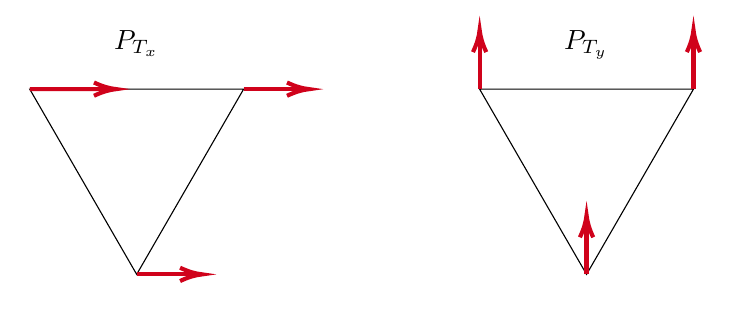
\begin{tikzpicture}[x=0.75pt,y=0.75pt,yscale=-0.75,xscale=0.75]
	%uncomment if require: \path (0,300); %set diagram left start at 0, and has height of 300
	
	%Shape: Regular Polygon [id:dp2523729045850933] 
	\draw   (108.43,108.54) -- (245.81,108.54) -- (177.12,227.52) -- cycle ;
	%Straight Lines [id:da9154552458698579] 
	\draw [color={rgb, 255:red, 208; green, 2; blue, 27 }  ,draw opacity=1 ][line width=1.5]    (245.81,108.54) -- (284.9,108.54) ;
	\draw [shift={(287.9,108.54)}, rotate = 180] [color={rgb, 255:red, 208; green, 2; blue, 27 }  ,draw opacity=1 ][line width=1.5]    (14.21,-4.28) .. controls (9.04,-1.82) and (4.3,-0.39) .. (0,0) .. controls (4.3,0.39) and (9.04,1.82) .. (14.21,4.28)   ;
	%Straight Lines [id:da35771830870091503] 
	\draw [color={rgb, 255:red, 208; green, 2; blue, 27 }  ,draw opacity=1 ][line width=1.5]    (108.43,108.54) -- (160.9,108.52) ;
	\draw [shift={(163.9,108.52)}, rotate = 539.98] [color={rgb, 255:red, 208; green, 2; blue, 27 }  ,draw opacity=1 ][line width=1.5]    (14.21,-4.28) .. controls (9.04,-1.82) and (4.3,-0.39) .. (0,0) .. controls (4.3,0.39) and (9.04,1.82) .. (14.21,4.28)   ;
	%Straight Lines [id:da7051277308014401] 
	\draw [color={rgb, 255:red, 208; green, 2; blue, 27 }  ,draw opacity=1 ][line width=1.5]    (177.12,227.52) -- (216.21,227.52) ;
	\draw [shift={(219.21,227.52)}, rotate = 180] [color={rgb, 255:red, 208; green, 2; blue, 27 }  ,draw opacity=1 ][line width=1.5]    (14.21,-4.28) .. controls (9.04,-1.82) and (4.3,-0.39) .. (0,0) .. controls (4.3,0.39) and (9.04,1.82) .. (14.21,4.28)   ;
	%Shape: Regular Polygon [id:dp5158025418972749] 
	\draw   (397.43,108.54) -- (534.81,108.54) -- (466.12,227.52) -- cycle ;
	%Straight Lines [id:da3274409935288376] 
	\draw [color={rgb, 255:red, 208; green, 2; blue, 27 }  ,draw opacity=1 ][line width=1.5]    (534.81,108.54) -- (534.81,73.52) ;
	\draw [shift={(534.81,70.52)}, rotate = 450] [color={rgb, 255:red, 208; green, 2; blue, 27 }  ,draw opacity=1 ][line width=1.5]    (14.21,-4.28) .. controls (9.04,-1.82) and (4.3,-0.39) .. (0,0) .. controls (4.3,0.39) and (9.04,1.82) .. (14.21,4.28)   ;
	%Straight Lines [id:da6576322833837083] 
	\draw [color={rgb, 255:red, 208; green, 2; blue, 27 }  ,draw opacity=1 ][line width=1.5]    (397.43,108.54) -- (397.43,73.52) ;
	\draw [shift={(397.43,70.52)}, rotate = 450] [color={rgb, 255:red, 208; green, 2; blue, 27 }  ,draw opacity=1 ][line width=1.5]    (14.21,-4.28) .. controls (9.04,-1.82) and (4.3,-0.39) .. (0,0) .. controls (4.3,0.39) and (9.04,1.82) .. (14.21,4.28)   ;
	%Straight Lines [id:da9472967991104069] 
	\draw [color={rgb, 255:red, 208; green, 2; blue, 27 }  ,draw opacity=1 ][line width=1.5]    (466.12,227.52) -- (466.12,192.5) ;
	\draw [shift={(466.12,189.5)}, rotate = 450] [color={rgb, 255:red, 208; green, 2; blue, 27 }  ,draw opacity=1 ][line width=1.5]    (14.21,-4.28) .. controls (9.04,-1.82) and (4.3,-0.39) .. (0,0) .. controls (4.3,0.39) and (9.04,1.82) .. (14.21,4.28)   ;
	
	% Text Node
	\draw (161,69.4) node [anchor=north west][inner sep=0.75pt]    {$P_{T_x}$};
	% Text Node
	\draw (450,69.4) node [anchor=north west][inner sep=0.75pt]    {$P_{T_y}$};
	
	
	\end{tikzpicture}
	\caption{The normal mode $P_{T_x}$ and $P_{T_y}$. }
\end{figure}

\subsection{Exercise 7.28}
\begin{equation*}
P=P_2-P_{T_x}-P_{T_y}=\begin{pmatrix}
\frac{1}{3} & 0 & -\frac{1}{6} & -\frac{\sqrt{3}}{6} & -\frac{1}{6} & \frac{\sqrt{3}}{6}\\
0 & \frac{1}{3} & \frac{\sqrt{3}}{6} & -\frac{1}{6} & -\frac{\sqrt{3}}{6} & -\frac{1}{6}\\
-\frac{1}{6} & \frac{\sqrt{3}}{6} & \frac{1}{3} & 0 & -\frac{1}{6} & -\frac{\sqrt{3}}{6}\\
-\frac{\sqrt{3}}{6} & -\frac{1}{6} & 0 & \frac{1}{3} & \frac{\sqrt{3}}{6} & -\frac{1}{6}\\
-\frac{1}{6} & -\frac{\sqrt{3}}{6} & -\frac{1}{6} & \frac{\sqrt{3}}{6} & \frac{1}{3} & 0\\
\frac{\sqrt{3}}{6} & -\frac{1}{6} & -\frac{\sqrt{3}}{6} & -\frac{1}{6} & 0 & \frac{1}{3}
\end{pmatrix}
\end{equation*}
with eigenvectors 
\begin{equation*}
v_1=\begin{pmatrix}
\frac{\sqrt{3}}{2} \\ -\frac{1}{2} \\ -\frac{\sqrt{3}}{2} \\ -\frac{1}{2} \\ 0 \\ 1
\end{pmatrix},\;\;v_2=\begin{pmatrix}
-\frac{1}{2} \\ -\frac{\sqrt{3}}{2} \\ -\frac{1}{2} \\\frac{\sqrt{3}}{2} \\ 1\\ 0
\end{pmatrix}
\end{equation*}
Thus we have the following normal mode: 
\begin{figure}[h]
	\centering
	\tikzset{every picture/.style={line width=0.75pt}} %set default line width to 0.75pt        
	
	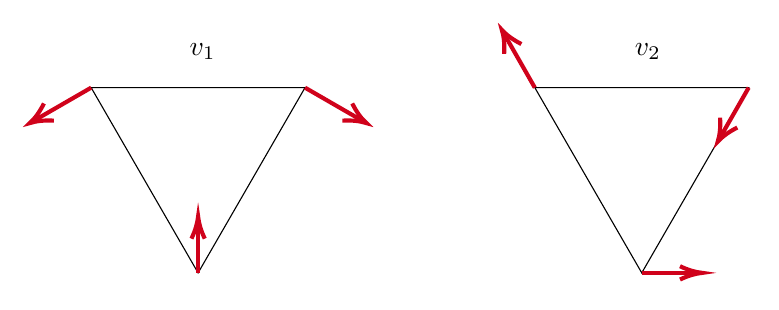
\begin{tikzpicture}[x=0.75pt,y=0.75pt,yscale=-0.75,xscale=0.75]
	%uncomment if require: \path (0,300); %set diagram left start at 0, and has height of 300
	
	%Shape: Regular Polygon [id:dp30982636233409777] 
	\draw   (115.43,94.54) -- (252.81,94.54) -- (184.12,213.52) -- cycle ;
	%Straight Lines [id:da8204299938869477] 
	\draw [color={rgb, 255:red, 208; green, 2; blue, 27 }  ,draw opacity=1 ][line width=1.5]    (252.81,94.54) -- (289.67,115.82) ;
	\draw [shift={(292.26,117.32)}, rotate = 210] [color={rgb, 255:red, 208; green, 2; blue, 27 }  ,draw opacity=1 ][line width=1.5]    (14.21,-6.37) .. controls (9.04,-2.99) and (4.3,-0.87) .. (0,0) .. controls (4.3,0.87) and (9.04,2.99) .. (14.21,6.37)   ;
	%Straight Lines [id:da4215332168225234] 
	\draw [color={rgb, 255:red, 208; green, 2; blue, 27 }  ,draw opacity=1 ][line width=1.5]    (115.43,94.54) -- (78.57,115.82) ;
	\draw [shift={(75.97,117.32)}, rotate = 330] [color={rgb, 255:red, 208; green, 2; blue, 27 }  ,draw opacity=1 ][line width=1.5]    (14.21,-6.37) .. controls (9.04,-2.99) and (4.3,-0.87) .. (0,0) .. controls (4.3,0.87) and (9.04,2.99) .. (14.21,6.37)   ;
	%Straight Lines [id:da5258505543680825] 
	\draw [color={rgb, 255:red, 208; green, 2; blue, 27 }  ,draw opacity=1 ][line width=1.5]    (184.12,213.52) -- (184.12,180.32) ;
	\draw [shift={(184.12,177.32)}, rotate = 450] [color={rgb, 255:red, 208; green, 2; blue, 27 }  ,draw opacity=1 ][line width=1.5]    (14.21,-4.28) .. controls (9.04,-1.82) and (4.3,-0.39) .. (0,0) .. controls (4.3,0.39) and (9.04,1.82) .. (14.21,4.28)   ;
	%Shape: Regular Polygon [id:dp4813723318499905] 
	\draw   (400.43,94.54) -- (537.81,94.54) -- (469.12,213.52) -- cycle ;
	%Straight Lines [id:da10435565556363513] 
	\draw [color={rgb, 255:red, 208; green, 2; blue, 27 }  ,draw opacity=1 ][line width=1.5]    (537.81,94.54) -- (519.39,126.72) ;
	\draw [shift={(517.9,129.32)}, rotate = 299.79] [color={rgb, 255:red, 208; green, 2; blue, 27 }  ,draw opacity=1 ][line width=1.5]    (14.21,-6.37) .. controls (9.04,-2.99) and (4.3,-0.87) .. (0,0) .. controls (4.3,0.87) and (9.04,2.99) .. (14.21,6.37)   ;
	%Straight Lines [id:da8726731235720666] 
	\draw [color={rgb, 255:red, 208; green, 2; blue, 27 }  ,draw opacity=1 ][line width=1.5]    (400.43,94.54) -- (380.69,59.95) ;
	\draw [shift={(379.21,57.34)}, rotate = 420.3] [color={rgb, 255:red, 208; green, 2; blue, 27 }  ,draw opacity=1 ][line width=1.5]    (14.21,-6.37) .. controls (9.04,-2.99) and (4.3,-0.87) .. (0,0) .. controls (4.3,0.87) and (9.04,2.99) .. (14.21,6.37)   ;
	%Straight Lines [id:da4859939486395286] 
	\draw [color={rgb, 255:red, 208; green, 2; blue, 27 }  ,draw opacity=1 ][line width=1.5]    (469.12,213.52) -- (504.9,213.52) ;
	\draw [shift={(507.9,213.52)}, rotate = 180] [color={rgb, 255:red, 208; green, 2; blue, 27 }  ,draw opacity=1 ][line width=1.5]    (14.21,-4.28) .. controls (9.04,-1.82) and (4.3,-0.39) .. (0,0) .. controls (4.3,0.39) and (9.04,1.82) .. (14.21,4.28)   ;
	
	% Text Node
	\draw (177,64.4) node [anchor=north west][inner sep=0.75pt]    {$v_{1}$};
	% Text Node
	\draw (463,64.4) node [anchor=north west][inner sep=0.75pt]    {$v_{2}$};
	
	
	\end{tikzpicture}
	\caption{The normal modes of $P=|v_1\rangle\langle v_1|+|v_2\rangle\langle v_2|$.}
\end{figure}


\subsection{Exercise 7.29}
The symmetry group of the system is $D_4$, which character table is given by 
\begin{equation*}
\begin{array}{c|c|ccccc|cc}
\Xhline{0.7pt}
D_4 & n_C & 1 & 1' & 1'' & 1''' & 2 & 4 & 4\otimes 2\\
\hline 
e & 1 & 1 & 1 & 1 & 1 & 2 & 4 & 8\\
-e=R^2 & 1 & 1 & 1 & 1 & 1 & -2 & 0 & 0\\
R,R^3 & 2 & 1 & -1 & -1 & 1 & 0 & 0 & 0\\
r_x, r_y & 2 & 1 & -1 & 1 & -1 & 0 & 0 & 0\\
d_1, d_2 & 2 & 1 & 1 & -1 & -1 & 0 & 2 & 0\\
\Xhline{0.7pt}
\end{array}
\end{equation*}
where in the last two column we include the restriction of the defining representation of $S_4$ (Noting that $D_4\subset S_4$ and $-e=(13)(24)$, $R=(1234)$, 
$R^3=(1432)$, $r_x=(12)(34)$, $r_y=(14)(23)$, $d_1=(24)$ and $d_2=(13)$.) and its tensor product with the defining representation 
of $D_4$. For the defination of the group elements, see the following picture: 

\begin{figure}[h]
	\centering
	\tikzset{every picture/.style={line width=0.75pt}} %set default line width to 0.75pt        
	
	\begin{tikzpicture}[x=0.75pt,y=0.75pt,yscale=-1,xscale=1]
	%uncomment if require: \path (0,300); %set diagram left start at 0, and has height of 300
	
	%Shape: Square [id:dp681453443617638] 
	\draw   (237,64.56) -- (399.44,64.56) -- (399.44,227) -- (237,227) -- cycle ;
	%Straight Lines [id:da6560351824166548] 
	\draw [color={rgb, 255:red, 144; green, 19; blue, 254 }  ,draw opacity=1 ] [dash pattern={on 4.5pt off 4.5pt}]  (399.44,64.56) -- (237,227) ;
	%Straight Lines [id:da1885713551675352] 
	\draw [color={rgb, 255:red, 144; green, 19; blue, 254 }  ,draw opacity=1 ] [dash pattern={on 4.5pt off 4.5pt}]  (399.44,227) -- (237,64.56) ;
	%Straight Lines [id:da43345347015242264] 
	\draw [color={rgb, 255:red, 144; green, 19; blue, 254 }  ,draw opacity=1 ] [dash pattern={on 4.5pt off 4.5pt}]  (318.22,64.56) -- (318.22,227) ;
	%Straight Lines [id:da6970636829569619] 
	\draw [color={rgb, 255:red, 144; green, 19; blue, 254 }  ,draw opacity=1 ] [dash pattern={on 4.5pt off 4.5pt}]  (399.44,145.78) -- (237,145.78) ;
	%Shape: Arc [id:dp41731453692456855] 
	\draw  [draw opacity=0] (406.46,35.39) .. controls (419.19,38.44) and (428.87,49.64) .. (429.42,63.37) .. controls (429.56,66.97) and (429.06,70.45) .. (428.02,73.69) -- (399.44,64.56) -- cycle ; \draw   (406.46,35.39) .. controls (419.19,38.44) and (428.87,49.64) .. (429.42,63.37) .. controls (429.56,66.97) and (429.06,70.45) .. (428.02,73.69) ;
	\draw   (413.62,45.58) .. controls (411.54,40.67) and (408.83,37.02) .. (405.52,34.62) .. controls (409.44,35.76) and (413.99,35.66) .. (419.14,34.3) ;
	
	% Text Node
	\draw (312.44,39.18) node [anchor=north west][inner sep=0.75pt]    {$r_{x}$};
	% Text Node
	\draw (404.22,134.96) node [anchor=north west][inner sep=0.75pt]    {$r_{y}$};
	% Text Node
	\draw (358,70.4) node [anchor=north west][inner sep=0.75pt]    {$d_{1}$};
	% Text Node
	\draw (260,71.4) node [anchor=north west][inner sep=0.75pt]    {$d_{2}$};
	% Text Node
	\draw (444,26.4) node [anchor=north west][inner sep=0.75pt]    {$R$};
	% Text Node
	\draw (405,48.4) node [anchor=north west][inner sep=0.75pt]    {$1$};
	% Text Node
	\draw (217,48.4) node [anchor=north west][inner sep=0.75pt]    {$2$};
	% Text Node
	\draw (222,227.4) node [anchor=north west][inner sep=0.75pt]    {$3$};
	% Text Node
	\draw (401.44,230.4) node [anchor=north west][inner sep=0.75pt]    {$4$};
	
	
	\end{tikzpicture}
	\caption{Definition of the group element of $D_4$}
\end{figure}

Noting that $r_y=r_xR^2$, $d_1=r_x R$, $d_2=r_xR^2$, we can write down the following representation matrices: 

For the defining representation of $D_4$, we have 
\begin{equation*}
\rho^2(e)=\begin{pmatrix}
1 & 0 \\ 0 & 1
\end{pmatrix}\;\;\rho^2(-e)=\begin{pmatrix}
-1 & 0 \\ 0 & -1
\end{pmatrix}\;\;\rho^2(R)=\begin{pmatrix}
0 & -1 \\ 1 & 0
\end{pmatrix}\;\;\rho^2(R^3)=\begin{pmatrix}
0 & 1 \\ -1 & 0
\end{pmatrix}
\end{equation*}
\begin{equation*}
\rho^2(r_x)=\begin{pmatrix}
-1 & 0\\ 0 & 1
\end{pmatrix}\;\;\rho^2(r_y)=\begin{pmatrix}
1 & 0 \\ 0 & -1
\end{pmatrix}\;\;\rho^2(d_1)=\begin{pmatrix}
0 & 1 \\ 1 & 0
\end{pmatrix}\;\;\rho^2(d_2)=\begin{pmatrix}
0 & -1 \\ -1 & 0
\end{pmatrix}
\end{equation*}

For the restriction of the defining representation of $S_4$, we have 
\begin{equation*}
\rho^4(e)=\begin{pmatrix}
1 & 0 & 0 & 0\\
0 & 1 & 0 & 0\\
0 & 0 & 1 & 0\\
0 & 0 & 0 & 1
\end{pmatrix}\;\;\rho^4(-e)=\begin{pmatrix}
0 & 0 & 1 & 0\\
0 & 0 & 0 & 1\\
1 & 0 & 0 & 0\\
0 & 1 & 0 & 0
\end{pmatrix}\;\;\rho^4(R)=\begin{pmatrix}
0 & 0 & 0 & 4\\
1 & 0 & 0 & 0\\
0 & 1 & 0 & 0\\
0 & 0 & 1 & 0
\end{pmatrix}
\end{equation*}
\begin{equation*}
\rho^4(R^3)=\begin{pmatrix}
0 & 1 & 0 & 0\\
0 & 0 & 1 & 0\\
0 & 0 & 0 & 1\\
1 & 0 & 0 & 0
\end{pmatrix}\;\;\rho^4(r_x)=\begin{pmatrix}
0 & 1 & 0 & 0\\
1 & 0 & 0 & 0\\
0 & 0 & 0 & 1\\
0 & 0 & 1 & 0
\end{pmatrix}\;\;\rho^4(r_y)=\begin{pmatrix}
0 & 0 & 0 & 1\\
0 & 0 & 1 & 0\\
0 & 1 & 0 & 0\\
1 & 0 & 0 & 0
\end{pmatrix}
\end{equation*}
\begin{equation*}
\rho^4(d_1)=\begin{pmatrix}
1 & 0 & 0 & 0\\
0 & 0 & 0 & 1\\
0 & 0 & 1 & 0\\
0 & 1 & 0 & 0
\end{pmatrix}\;\;\rho^4(d_2)=\begin{pmatrix}
0 & 0 & 1 & 0\\
0 & 1 & 0 & 0\\
1 & 0 & 0 & 0\\
0 & 0 & 0 & 1
\end{pmatrix}
\end{equation*}

Noting that $4=1\oplus 1'\oplus 2$: 
\begin{align*}
&n_1=n_{1'}=\frac{1}{8}(1\times 4+2\times1\times 2)=1\\
&n_2=\frac{1}{8}(2\times 4+0)=1
\end{align*}
and $4\otimes 2=1\oplus 1'\oplus1''\oplus1'''\oplus2\oplus 2$ (and thus $4\otimes 2$ is equivalent to the regular representation of $D_4$):
\begin{align*}
&n_1=n_{1'}=n_{1''}=n_{1'''}=\frac{1}{8}(1\times 8+0)=1\\
&n_2=\frac{1}{8}(2\times 8)=2
\end{align*}

Now lets define the projectors: 
\begin{equation*}
P_1=\frac{1}{8}\sum_{g\in G}\chi^1(g)^*\rho^{4\otimes 2}(g)=|1\rangle\langle 1|\;\;\text{with}\;\;|1\rangle=\frac{1}{2\sqrt{2}}\begin{pmatrix}
-1\\-1\\1\\-1\\1\\1\\-1\\1
\end{pmatrix}
\end{equation*}
Simiarly, we find 
\begin{equation*}
P_{1'}=|1'\rangle\langle1'|\;\;\text{with}\;\;|1'\rangle=\frac{1}{2\sqrt{2}}\begin{pmatrix}
1\\1\\1\\-1\\-1\\-1\\-1\\1
\end{pmatrix}
\end{equation*}
\begin{equation*}
P_{1''}=|1''\rangle\langle1''|\;\;\text{with}\;\;|1''\rangle=\frac{1}{2\sqrt{2}}\begin{pmatrix}
1\\-1\\-1\\-1\\-1\\1\\1\\1
\end{pmatrix}
\end{equation*}
\begin{equation*}
P_{1'''}=|1'''\rangle\langle1'|\;\;\text{with}\;\;|1'''\rangle=\frac{1}{2\sqrt{2}}\begin{pmatrix}
-1\\1\\-1\\-1\\1\\-1\\1\\1
\end{pmatrix}
\end{equation*}

Just like the case where three masses connected by three springs, we have projectors corresponding to the constant translation
\begin{equation*}
P_{T_x}=|T_x\rangle\langle T_x|\;\;\text{with}\;\;|T_x\rangle=\begin{pmatrix}
1\\0\\1\\0\\1\\0\\1\\0
\end{pmatrix}\;\;\text{and}\;\;P_{T_y}=|T_y\rangle\langle T_y|\;\;\text{with}\;\;|T_y\rangle=\begin{pmatrix}
0\\1\\0\\1\\0\\1\\0\\1
\end{pmatrix}
\end{equation*} 
and 
\begin{equation*}
P_2=\frac{2}{8}\sum_{g\in G}\chi^2(g)^*\rho^{4\otimes 2}(g)=\frac{1}{2}\begin{pmatrix}
\mathbf 1_{4\times 4} &  \mathbf 1_{4\times 4}\\
\mathbf 1_{4\times 4} & \mathbf 1_{4\times 4}
\end{pmatrix}
\end{equation*}
Thus we have 
\begin{equation*}
P=P_2-P_{T_x}-P_{T_y}=|2'\rangle\langle 2'|+|2''\rangle\langle 2''|\;\;\text{with}\;\;|2'\rangle=\frac{1}{2}\begin{pmatrix}
0\\-1\\0\\1\\0\\-1\\0\\1
\end{pmatrix}\;\;\text{and}\;\;|2''\rangle=\frac{1}{2}\begin{pmatrix}
-1\\0\\1\\0\\-1\\0\\1\\0
\end{pmatrix}
\end{equation*}
The zero modes are given by $P_{T_x}$, $P_{T_y}$ and $P_{1'''}$. The corresponding normal modes of the above projectors are listed in the following 
diagram: 

\begin{figure}[h]
	\centering
	\tikzset{every picture/.style={line width=0.75pt}} %set default line width to 0.75pt        
	
	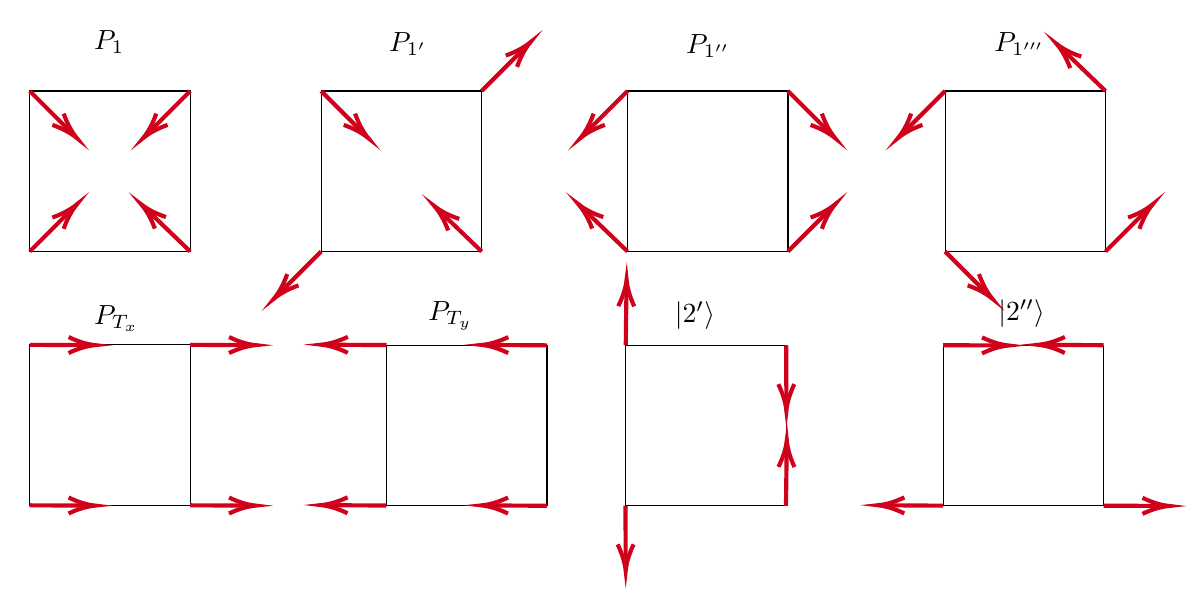
\begin{tikzpicture}[x=0.75pt,y=0.75pt,yscale=-0.9,xscale=0.9]
	%uncomment if require: \path (0,319); %set diagram left start at 0, and has height of 319
	
	%Shape: Square [id:dp8970270720789542] 
	\draw   (31,50.04) -- (116.9,50.04) -- (116.9,135.94) -- (31,135.94) -- cycle ;
	%Straight Lines [id:da0151022565185015] 
	\draw [color={rgb, 255:red, 208; green, 2; blue, 27 }  ,draw opacity=1 ][line width=1.5]    (116.9,50.04) -- (93.84,73.1) ;
	\draw [shift={(91.72,75.22)}, rotate = 315] [color={rgb, 255:red, 208; green, 2; blue, 27 }  ,draw opacity=1 ][line width=1.5]    (14.21,-4.28) .. controls (9.04,-1.82) and (4.3,-0.39) .. (0,0) .. controls (4.3,0.39) and (9.04,1.82) .. (14.21,4.28)   ;
	%Straight Lines [id:da4444343399892554] 
	\draw [color={rgb, 255:red, 208; green, 2; blue, 27 }  ,draw opacity=1 ][line width=1.5]    (31,50.04) -- (54.06,73.1) ;
	\draw [shift={(56.18,75.22)}, rotate = 225] [color={rgb, 255:red, 208; green, 2; blue, 27 }  ,draw opacity=1 ][line width=1.5]    (14.21,-4.28) .. controls (9.04,-1.82) and (4.3,-0.39) .. (0,0) .. controls (4.3,0.39) and (9.04,1.82) .. (14.21,4.28)   ;
	%Straight Lines [id:da28469078005001824] 
	\draw [color={rgb, 255:red, 208; green, 2; blue, 27 }  ,draw opacity=1 ][line width=1.5]    (31,135.94) -- (54.06,112.88) ;
	\draw [shift={(56.18,110.76)}, rotate = 495] [color={rgb, 255:red, 208; green, 2; blue, 27 }  ,draw opacity=1 ][line width=1.5]    (14.21,-4.28) .. controls (9.04,-1.82) and (4.3,-0.39) .. (0,0) .. controls (4.3,0.39) and (9.04,1.82) .. (14.21,4.28)   ;
	%Straight Lines [id:da5192443969361966] 
	\draw [color={rgb, 255:red, 208; green, 2; blue, 27 }  ,draw opacity=1 ][line width=1.5]    (116.9,135.94) -- (92.88,112.84) ;
	\draw [shift={(90.72,110.76)}, rotate = 403.88] [color={rgb, 255:red, 208; green, 2; blue, 27 }  ,draw opacity=1 ][line width=1.5]    (14.21,-4.28) .. controls (9.04,-1.82) and (4.3,-0.39) .. (0,0) .. controls (4.3,0.39) and (9.04,1.82) .. (14.21,4.28)   ;
	%Shape: Square [id:dp15480171534901044] 
	\draw   (187,50.04) -- (272.9,50.04) -- (272.9,135.94) -- (187,135.94) -- cycle ;
	%Straight Lines [id:da499468080673799] 
	\draw [color={rgb, 255:red, 208; green, 2; blue, 27 }  ,draw opacity=1 ][line width=1.5]    (272.9,50.04) -- (296.78,26.16) ;
	\draw [shift={(298.9,24.04)}, rotate = 495] [color={rgb, 255:red, 208; green, 2; blue, 27 }  ,draw opacity=1 ][line width=1.5]    (14.21,-4.28) .. controls (9.04,-1.82) and (4.3,-0.39) .. (0,0) .. controls (4.3,0.39) and (9.04,1.82) .. (14.21,4.28)   ;
	%Straight Lines [id:da5977494433822494] 
	\draw [color={rgb, 255:red, 208; green, 2; blue, 27 }  ,draw opacity=1 ][line width=1.5]    (187,135.94) -- (163.94,159) ;
	\draw [shift={(161.82,161.12)}, rotate = 315] [color={rgb, 255:red, 208; green, 2; blue, 27 }  ,draw opacity=1 ][line width=1.5]    (14.21,-4.28) .. controls (9.04,-1.82) and (4.3,-0.39) .. (0,0) .. controls (4.3,0.39) and (9.04,1.82) .. (14.21,4.28)   ;
	%Straight Lines [id:da3184368457016611] 
	\draw [color={rgb, 255:red, 208; green, 2; blue, 27 }  ,draw opacity=1 ][line width=1.5]    (272.9,135.94) -- (249.88,113.84) ;
	\draw [shift={(247.72,111.76)}, rotate = 403.84000000000003] [color={rgb, 255:red, 208; green, 2; blue, 27 }  ,draw opacity=1 ][line width=1.5]    (14.21,-4.28) .. controls (9.04,-1.82) and (4.3,-0.39) .. (0,0) .. controls (4.3,0.39) and (9.04,1.82) .. (14.21,4.28)   ;
	%Straight Lines [id:da303562769527026] 
	\draw [color={rgb, 255:red, 208; green, 2; blue, 27 }  ,draw opacity=1 ][line width=1.5]    (187,50.04) -- (210.06,73.1) ;
	\draw [shift={(212.18,75.22)}, rotate = 225] [color={rgb, 255:red, 208; green, 2; blue, 27 }  ,draw opacity=1 ][line width=1.5]    (14.21,-4.28) .. controls (9.04,-1.82) and (4.3,-0.39) .. (0,0) .. controls (4.3,0.39) and (9.04,1.82) .. (14.21,4.28)   ;
	%Shape: Square [id:dp6016609954732794] 
	\draw   (351,50.04) -- (436.9,50.04) -- (436.9,135.94) -- (351,135.94) -- cycle ;
	%Straight Lines [id:da7969559161770325] 
	\draw [color={rgb, 255:red, 208; green, 2; blue, 27 }  ,draw opacity=1 ][line width=1.5]    (436.9,135.94) -- (459.96,112.88) ;
	\draw [shift={(462.08,110.76)}, rotate = 495] [color={rgb, 255:red, 208; green, 2; blue, 27 }  ,draw opacity=1 ][line width=1.5]    (14.21,-4.28) .. controls (9.04,-1.82) and (4.3,-0.39) .. (0,0) .. controls (4.3,0.39) and (9.04,1.82) .. (14.21,4.28)   ;
	%Straight Lines [id:da7129887876640044] 
	\draw [color={rgb, 255:red, 208; green, 2; blue, 27 }  ,draw opacity=1 ][line width=1.5]    (436.9,50.04) -- (459.96,73.1) ;
	\draw [shift={(462.08,75.22)}, rotate = 225] [color={rgb, 255:red, 208; green, 2; blue, 27 }  ,draw opacity=1 ][line width=1.5]    (14.21,-4.28) .. controls (9.04,-1.82) and (4.3,-0.39) .. (0,0) .. controls (4.3,0.39) and (9.04,1.82) .. (14.21,4.28)   ;
	%Straight Lines [id:da7282980446039216] 
	\draw [color={rgb, 255:red, 208; green, 2; blue, 27 }  ,draw opacity=1 ][line width=1.5]    (351,50.04) -- (327.94,73.1) ;
	\draw [shift={(325.82,75.22)}, rotate = 315] [color={rgb, 255:red, 208; green, 2; blue, 27 }  ,draw opacity=1 ][line width=1.5]    (14.21,-4.28) .. controls (9.04,-1.82) and (4.3,-0.39) .. (0,0) .. controls (4.3,0.39) and (9.04,1.82) .. (14.21,4.28)   ;
	%Straight Lines [id:da39302056019095843] 
	\draw [color={rgb, 255:red, 208; green, 2; blue, 27 }  ,draw opacity=1 ][line width=1.5]    (351,135.94) -- (326.98,112.84) ;
	\draw [shift={(324.82,110.76)}, rotate = 403.88] [color={rgb, 255:red, 208; green, 2; blue, 27 }  ,draw opacity=1 ][line width=1.5]    (14.21,-4.28) .. controls (9.04,-1.82) and (4.3,-0.39) .. (0,0) .. controls (4.3,0.39) and (9.04,1.82) .. (14.21,4.28)   ;
	%Shape: Square [id:dp3188258967399331] 
	\draw   (521,50.04) -- (606.9,50.04) -- (606.9,135.94) -- (521,135.94) -- cycle ;
	%Straight Lines [id:da41897436392370113] 
	\draw [color={rgb, 255:red, 208; green, 2; blue, 27 }  ,draw opacity=1 ][line width=1.5]    (606.9,50.04) -- (582.88,26.94) ;
	\draw [shift={(580.72,24.86)}, rotate = 403.88] [color={rgb, 255:red, 208; green, 2; blue, 27 }  ,draw opacity=1 ][line width=1.5]    (14.21,-4.28) .. controls (9.04,-1.82) and (4.3,-0.39) .. (0,0) .. controls (4.3,0.39) and (9.04,1.82) .. (14.21,4.28)   ;
	%Straight Lines [id:da41853272213715975] 
	\draw [color={rgb, 255:red, 208; green, 2; blue, 27 }  ,draw opacity=1 ][line width=1.5]    (521,50.04) -- (497.94,73.1) ;
	\draw [shift={(495.82,75.22)}, rotate = 315] [color={rgb, 255:red, 208; green, 2; blue, 27 }  ,draw opacity=1 ][line width=1.5]    (14.21,-4.28) .. controls (9.04,-1.82) and (4.3,-0.39) .. (0,0) .. controls (4.3,0.39) and (9.04,1.82) .. (14.21,4.28)   ;
	%Straight Lines [id:da20977227582760616] 
	\draw [color={rgb, 255:red, 208; green, 2; blue, 27 }  ,draw opacity=1 ][line width=1.5]    (521,135.94) -- (544.06,159) ;
	\draw [shift={(546.18,161.12)}, rotate = 225] [color={rgb, 255:red, 208; green, 2; blue, 27 }  ,draw opacity=1 ][line width=1.5]    (14.21,-4.28) .. controls (9.04,-1.82) and (4.3,-0.39) .. (0,0) .. controls (4.3,0.39) and (9.04,1.82) .. (14.21,4.28)   ;
	%Straight Lines [id:da9034015429758435] 
	\draw [color={rgb, 255:red, 208; green, 2; blue, 27 }  ,draw opacity=1 ][line width=1.5]    (606.9,135.94) -- (629.96,112.88) ;
	\draw [shift={(632.08,110.76)}, rotate = 495] [color={rgb, 255:red, 208; green, 2; blue, 27 }  ,draw opacity=1 ][line width=1.5]    (14.21,-4.28) .. controls (9.04,-1.82) and (4.3,-0.39) .. (0,0) .. controls (4.3,0.39) and (9.04,1.82) .. (14.21,4.28)   ;
	%Shape: Square [id:dp3621736210918416] 
	\draw   (31,185.94) -- (116.9,185.94) -- (116.9,271.84) -- (31,271.84) -- cycle ;
	%Straight Lines [id:da02646542305163946] 
	\draw [color={rgb, 255:red, 208; green, 2; blue, 27 }  ,draw opacity=1 ][line width=1.5]    (31,185.94) -- (63,186.09) ;
	\draw [shift={(66,186.1)}, rotate = 180.26] [color={rgb, 255:red, 208; green, 2; blue, 27 }  ,draw opacity=1 ][line width=1.5]    (14.21,-4.28) .. controls (9.04,-1.82) and (4.3,-0.39) .. (0,0) .. controls (4.3,0.39) and (9.04,1.82) .. (14.21,4.28)   ;
	%Straight Lines [id:da4228996004933907] 
	\draw [color={rgb, 255:red, 208; green, 2; blue, 27 }  ,draw opacity=1 ][line width=1.5]    (116.9,185.94) -- (148.9,186.09) ;
	\draw [shift={(151.9,186.1)}, rotate = 180.26] [color={rgb, 255:red, 208; green, 2; blue, 27 }  ,draw opacity=1 ][line width=1.5]    (14.21,-4.28) .. controls (9.04,-1.82) and (4.3,-0.39) .. (0,0) .. controls (4.3,0.39) and (9.04,1.82) .. (14.21,4.28)   ;
	%Straight Lines [id:da01301021353776921] 
	\draw [color={rgb, 255:red, 208; green, 2; blue, 27 }  ,draw opacity=1 ][line width=1.5]    (116.9,271.84) -- (148.9,271.99) ;
	\draw [shift={(151.9,272)}, rotate = 180.26] [color={rgb, 255:red, 208; green, 2; blue, 27 }  ,draw opacity=1 ][line width=1.5]    (14.21,-4.28) .. controls (9.04,-1.82) and (4.3,-0.39) .. (0,0) .. controls (4.3,0.39) and (9.04,1.82) .. (14.21,4.28)   ;
	%Straight Lines [id:da6177628405648239] 
	\draw [color={rgb, 255:red, 208; green, 2; blue, 27 }  ,draw opacity=1 ][line width=1.5]    (31,271.84) -- (63,271.99) ;
	\draw [shift={(66,272)}, rotate = 180.26] [color={rgb, 255:red, 208; green, 2; blue, 27 }  ,draw opacity=1 ][line width=1.5]    (14.21,-4.28) .. controls (9.04,-1.82) and (4.3,-0.39) .. (0,0) .. controls (4.3,0.39) and (9.04,1.82) .. (14.21,4.28)   ;
	%Shape: Square [id:dp0949585162412383] 
	\draw   (307.9,272.03) -- (222,272.03) -- (222,186.13) -- (307.9,186.13) -- cycle ;
	%Straight Lines [id:da3589570624707785] 
	\draw [color={rgb, 255:red, 208; green, 2; blue, 27 }  ,draw opacity=1 ][line width=1.5]    (307.83,272.09) -- (275.83,271.9) ;
	\draw [shift={(272.83,271.88)}, rotate = 360.35] [color={rgb, 255:red, 208; green, 2; blue, 27 }  ,draw opacity=1 ][line width=1.5]    (14.21,-4.28) .. controls (9.04,-1.82) and (4.3,-0.39) .. (0,0) .. controls (4.3,0.39) and (9.04,1.82) .. (14.21,4.28)   ;
	%Straight Lines [id:da1491431470598219] 
	\draw [color={rgb, 255:red, 208; green, 2; blue, 27 }  ,draw opacity=1 ][line width=1.5]    (221.93,271.96) -- (189.93,271.76) ;
	\draw [shift={(186.93,271.74)}, rotate = 360.35] [color={rgb, 255:red, 208; green, 2; blue, 27 }  ,draw opacity=1 ][line width=1.5]    (14.21,-4.28) .. controls (9.04,-1.82) and (4.3,-0.39) .. (0,0) .. controls (4.3,0.39) and (9.04,1.82) .. (14.21,4.28)   ;
	%Straight Lines [id:da7422046381025462] 
	\draw [color={rgb, 255:red, 208; green, 2; blue, 27 }  ,draw opacity=1 ][line width=1.5]    (222.07,186.06) -- (190.07,185.86) ;
	\draw [shift={(187.07,185.85)}, rotate = 360.35] [color={rgb, 255:red, 208; green, 2; blue, 27 }  ,draw opacity=1 ][line width=1.5]    (14.21,-4.28) .. controls (9.04,-1.82) and (4.3,-0.39) .. (0,0) .. controls (4.3,0.39) and (9.04,1.82) .. (14.21,4.28)   ;
	%Straight Lines [id:da8739567136304769] 
	\draw [color={rgb, 255:red, 208; green, 2; blue, 27 }  ,draw opacity=1 ][line width=1.5]    (307.97,186.2) -- (275.97,186) ;
	\draw [shift={(272.97,185.98)}, rotate = 360.35] [color={rgb, 255:red, 208; green, 2; blue, 27 }  ,draw opacity=1 ][line width=1.5]    (14.21,-4.28) .. controls (9.04,-1.82) and (4.3,-0.39) .. (0,0) .. controls (4.3,0.39) and (9.04,1.82) .. (14.21,4.28)   ;
	%Shape: Square [id:dp8403865403319646] 
	\draw   (435.9,272.03) -- (350,272.03) -- (350,186.13) -- (435.9,186.13) -- cycle ;
	%Straight Lines [id:da3603185473922581] 
	\draw [color={rgb, 255:red, 208; green, 2; blue, 27 }  ,draw opacity=1 ][line width=1.5]    (350.07,186.06) -- (350.47,154.06) ;
	\draw [shift={(350.51,151.06)}, rotate = 450.72] [color={rgb, 255:red, 208; green, 2; blue, 27 }  ,draw opacity=1 ][line width=1.5]    (14.21,-4.28) .. controls (9.04,-1.82) and (4.3,-0.39) .. (0,0) .. controls (4.3,0.39) and (9.04,1.82) .. (14.21,4.28)   ;
	%Straight Lines [id:da23107211401312355] 
	\draw [color={rgb, 255:red, 208; green, 2; blue, 27 }  ,draw opacity=1 ][line width=1.5]    (435.97,186.2) -- (436.04,218.2) ;
	\draw [shift={(436.05,221.2)}, rotate = 269.86] [color={rgb, 255:red, 208; green, 2; blue, 27 }  ,draw opacity=1 ][line width=1.5]    (14.21,-4.28) .. controls (9.04,-1.82) and (4.3,-0.39) .. (0,0) .. controls (4.3,0.39) and (9.04,1.82) .. (14.21,4.28)   ;
	%Straight Lines [id:da17161544162322206] 
	\draw [color={rgb, 255:red, 208; green, 2; blue, 27 }  ,draw opacity=1 ][line width=1.5]    (349.93,271.96) -- (350.01,303.96) ;
	\draw [shift={(350.02,306.96)}, rotate = 269.86] [color={rgb, 255:red, 208; green, 2; blue, 27 }  ,draw opacity=1 ][line width=1.5]    (14.21,-4.28) .. controls (9.04,-1.82) and (4.3,-0.39) .. (0,0) .. controls (4.3,0.39) and (9.04,1.82) .. (14.21,4.28)   ;
	%Straight Lines [id:da43768353864712495] 
	\draw [color={rgb, 255:red, 208; green, 2; blue, 27 }  ,draw opacity=1 ][line width=1.5]    (435.83,272.09) -- (436.24,240.1) ;
	\draw [shift={(436.27,237.1)}, rotate = 450.72] [color={rgb, 255:red, 208; green, 2; blue, 27 }  ,draw opacity=1 ][line width=1.5]    (14.21,-4.28) .. controls (9.04,-1.82) and (4.3,-0.39) .. (0,0) .. controls (4.3,0.39) and (9.04,1.82) .. (14.21,4.28)   ;
	%Shape: Square [id:dp6131302749475134] 
	\draw   (605.9,272.03) -- (520,272.03) -- (520,186.13) -- (605.9,186.13) -- cycle ;
	%Straight Lines [id:da2818506454540961] 
	\draw [color={rgb, 255:red, 208; green, 2; blue, 27 }  ,draw opacity=1 ][line width=1.5]    (520,186.13) -- (552,186.27) ;
	\draw [shift={(555,186.29)}, rotate = 180.26] [color={rgb, 255:red, 208; green, 2; blue, 27 }  ,draw opacity=1 ][line width=1.5]    (14.21,-4.28) .. controls (9.04,-1.82) and (4.3,-0.39) .. (0,0) .. controls (4.3,0.39) and (9.04,1.82) .. (14.21,4.28)   ;
	%Straight Lines [id:da18003517545572412] 
	\draw [color={rgb, 255:red, 208; green, 2; blue, 27 }  ,draw opacity=1 ][line width=1.5]    (605.9,186.13) -- (573.9,185.93) ;
	\draw [shift={(570.9,185.91)}, rotate = 360.35] [color={rgb, 255:red, 208; green, 2; blue, 27 }  ,draw opacity=1 ][line width=1.5]    (14.21,-4.28) .. controls (9.04,-1.82) and (4.3,-0.39) .. (0,0) .. controls (4.3,0.39) and (9.04,1.82) .. (14.21,4.28)   ;
	%Straight Lines [id:da8301712420696796] 
	\draw [color={rgb, 255:red, 208; green, 2; blue, 27 }  ,draw opacity=1 ][line width=1.5]    (520,272.03) -- (488,271.83) ;
	\draw [shift={(485,271.81)}, rotate = 360.35] [color={rgb, 255:red, 208; green, 2; blue, 27 }  ,draw opacity=1 ][line width=1.5]    (14.21,-4.28) .. controls (9.04,-1.82) and (4.3,-0.39) .. (0,0) .. controls (4.3,0.39) and (9.04,1.82) .. (14.21,4.28)   ;
	%Straight Lines [id:da1505951778107828] 
	\draw [color={rgb, 255:red, 208; green, 2; blue, 27 }  ,draw opacity=1 ][line width=1.5]    (605.9,272.03) -- (637.9,272.17) ;
	\draw [shift={(640.9,272.19)}, rotate = 180.26] [color={rgb, 255:red, 208; green, 2; blue, 27 }  ,draw opacity=1 ][line width=1.5]    (14.21,-4.28) .. controls (9.04,-1.82) and (4.3,-0.39) .. (0,0) .. controls (4.3,0.39) and (9.04,1.82) .. (14.21,4.28)   ;
	
	% Text Node
	\draw (64,16.44) node [anchor=north west][inner sep=0.75pt]    {$P_{1}$};
	% Text Node
	\draw (222,17.4) node [anchor=north west][inner sep=0.75pt]    {$P_{1'}$};
	% Text Node
	\draw (381,18.4) node [anchor=north west][inner sep=0.75pt]    {$P_{1''}$};
	% Text Node
	\draw (546,17.4) node [anchor=north west][inner sep=0.75pt]    {$P_{1'''}$};
	% Text Node
	\draw (64,163.4) node [anchor=north west][inner sep=0.75pt]    {$P_{T_{x}}$};
	% Text Node
	\draw (243,161.4) node [anchor=north west][inner sep=0.75pt]    {$P_{T_{y}}$};
	% Text Node
	\draw (375,161.4) node [anchor=north west][inner sep=0.75pt]    {$| 2'\rangle $};
	% Text Node
	\draw (548.18,160.52) node [anchor=north west][inner sep=0.75pt]    {$| 2''\rangle $};
	
	
	\end{tikzpicture}
	\caption{The normal modes.}
\end{figure}


\subsection{Exercise 7.30}
Noting that $\chi^{\mu\otimes\nu}(g)=\chi^\mu(g)\chi^\nu(g)$, we have 
\begin{align*}
&n_1=\frac{1}{6}\sum_{A=1}^3n_A\chi_A^1(g)\big[\chi^2(g)\big]^2=\frac{1}{6}(1\times 1\times 2^2+3\times 1\times 0^2+2\times 1\times (-1)^2)=1\\
&n_{\bar 1}=\frac{1}{6}\sum_{A=1}^3n_A\chi_A^{\bar 1}(g)\big[\chi^2(g)\big]^2=\frac{1}{6}(1\times 1\times 2^2+3\times(-1)\times 0^2+2\times 1\times (-1)^2)=1\\
&n_2=\frac{1}{6}\sum_{A=1}^3n_A\chi_A^2(g)\big[\chi^2(g)\big]^2=\frac{1}{6}(1\times 2\times 2^2+3\times 0\times 0^2+2\times (-1)\times (-1)^2)=1
\end{align*}
Thus we have $2\otimes 2=1\oplus\bar 1\oplus 2$. 
\subsection{Exercise 7.31}
\begin{align*}
&\langle j_1,m_1;j_2,m_1|\mathcal O|j_1,m_1';j_2,m_2'\rangle\\
={}&\sum_{\alpha,J,m}\sum_{\beta,J',m'}\langle j_1,m_1;j_2,m_2|J,m\rangle_\alpha{}_\beta\!\langle J',m'|j_1,m_1';j_2,m_2'\rangle\underbrace{{}_{\alpha}\!\langle J,m|\mathcal{O}|J',m'\rangle_\beta}_{\delta_{JJ'}\delta_{mm'}f_J(\alpha,\beta)}\\
={}&\sum_{\alpha,\beta,J,m}C_{j_1j_2m_1m_2}^{\alpha Jm}(C_{j_1j_2m_1'm_2'}^{\beta Jm})^*f_J(\alpha,\beta)
\end{align*}

\section{Fourier and Laplace Transform, and Differential Equations}
\subsection{Exercise 8.1}
We have 
\begin{align*}
|k|^m|\tilde{f}(k)|&=\frac{1}{2l}\left|\int_{-l}^lk^mf(x)\mathrm{e}^{-\mathrm{i}k\pi x/l}\mathrm{d}x\right|\\
&=\frac{1}{2l}\frac{l}{\pi}\left|\int_{-l}^l k^{m-1}f'(x)\mathrm{e}^{-\mathrm{i}k\pi x/l}\mathrm{d}x\right|\\
&\cdots \\
&=\frac{1}{2l}\left|\left(\frac{l}{\pi}\right)^m\int_{-l}^{l}f^{(m)}(x)\mathrm{e}^{-\mathrm{i}k\pi x/l}\mathrm{d}x\right|\\
&\le\frac{1}{2l}\left(\frac{l}{\pi}\right)^m\cdot 2l\max_{x\in[-l,l]}|f^{(m)}(x)|\;\;\forall\;k\in\mathbb Z
\end{align*}
Therefore we have $\sup_{k\in\mathbb Z}|k|^m|\tilde{f}(k)|<\infty$. 

\subsection{Exercise 8.2}
For two function $f,g\in L^2(S^1)$, the convolution defined as 
\begin{equation*}
\big[f\star_{2l}g\big](x)=\int_{-l}^lf(x')g(x-x')\mathrm{d}x'
\end{equation*}
Then 
\begin{align*}
\widetilde{f\star_{2l}g}(k)&=\frac{1}{2l}\int_{-l}^l(f\star_{2l}g)(x)\mathrm{e}^{-\mathrm{i}k\pi x/l}\mathrm{d}x\\
&=\frac{1}{2l}\int_{-l}^l\mathrm{d}x\int_{-l}^l\mathrm{d}x'\;f(x')g(x-x')\mathrm{e}^{-\mathrm{i}k\pi(x'+x-x')/l}\\
&=2l\tilde{f}(k)\tilde{g}(k)
\end{align*}
If we further define the distrete convolution as 
\begin{equation*}
\left(\tilde{f}\star\tilde{g}\right)(k)=\sum_{k'\in\mathbb Z}\tilde{f}(k')\tilde{g}(k-k')
\end{equation*}
Then we have
\begin{equation*}
\left(\tilde{f}\star\tilde{g}\right)(k)=\frac{1}{4l^2}\int_{-l}^l\mathrm{d}x\int_{-l}^l\mathrm{d}x'\sum_{k'\in\mathbb Z}f(x)\mathrm{e}^{-\mathrm{i}k'\pi x/l}g(x')\mathrm{e}^{-\mathrm{i}(k-k')\pi x'/l}
\end{equation*}
Consider 
\begin{equation*}
\widetilde{\delta(x)}(k)=\frac{1}{2l}\int_{-l}^l\delta(x)\mathrm{e}^{-\mathrm{i}k\pi x/l}\mathrm{d}x=\frac{1}{2l}
\end{equation*}
Thus we have 
\begin{equation*}
\sum_{k\in\mathbb Z}\frac{1}{2l}\mathrm{e}^{\mathrm{i}k\pi x/l}=\delta(x)\;\;\Rightarrow\;\;\sum_{k'\in\mathbb Z}\mathrm{e}^{\mathrm{i}k'\pi(x'-x)/l}=2l\delta(x'-x)
\end{equation*}
which implies that 
\begin{align*}
\left(\tilde{f}\star\tilde{g}\right)(k)&=\frac{1}{4l^2}\int_{-l}^l\mathrm{d}x\int_{-l}^l\mathrm{d}x'\;f(x)\mathrm{e}^{-\mathrm{i}k\pi x'/l}g(x')\cdot 2l\delta(x'-x)\\
&=\frac{1}{2l}\int_{-l}^l f(x)g(x)\mathrm{e}^{-\mathrm{i}k\pi x/l}\mathrm{d}x\\
&=\widetilde{f\cdot g}(k)
\end{align*}

\subsection{Exercise 8.3}
\subsubsection*{8.3.1} As $f(\mathbf R+\mathbf r)=f(\mathbf r)$, we have $g(x_1,x_2,x_3)=g(x_1+a_1,x_2+a_2,x_3+a_3)$. Hence we have the Fourier expansion 
\begin{equation*}
g(x_1,x_2,x_3)=\sum_{m_1,m_2,m_3\in\mathbb Z}h(m_1,m_2,m_3)\cdot\mathrm{e}^{\mathrm{i}2\pi\left(\frac{m_1x_1}{a_1}+\frac{m_2x_2}{a_2}+\frac{m_3x_3}{a_3}\right)}
\end{equation*}
and the coefficients are given by 
\begin{equation*}
h(m_1,m_2,m_3)=\frac{1}{a_1a_2a_3}\int_0^{a_1}\int_0^{a_2}\int_0^{a_3}\mathrm{d}x_1\mathrm{d}x_2\mathrm{d}x_3\;g(x_1,x_2,x_3)\mathrm{e}^{-\mathrm{i}2\pi\left(\frac{m_1x_1}{a_1}+\frac{m_2x_2}{a_2}+\frac{m_3x_3}{a_3}\right)}
\end{equation*}

\subsubsection*{8.3.2} Let $\mathbf G=m_1\mathbf g_1+m_2\mathbf g_2+m_3\mathbf g_3$ with $\mathbf g_i\cdot\mathbf a_j=2\pi\delta_{ij}$, $m_1,m_2,m_3\in\mathbb Z$. 
Then we have 
\begin{equation*}
\mathbf G\cdot\mathbf r=\sum_{i=1}^3m_i\mathbf g_i\cdot\sum_{j=1}^3 x_j\frac{\mathbf a_j}{a_j}=2\pi\left(\frac{m_1x_1}{a_1}+\frac{m_2x_2}{a_2}+\frac{m_3x_3}{a_3}\right)
\end{equation*}
Therefore 
\begin{equation*}
h(\mathbf G)=h(m_1,m_2,m_3)=\int_0^{a_1}\frac{\mathrm{d}x_1}{a_1}\int_0^{a_2}\frac{\mathrm{d}x_2}{a_2}\int_0^{a_3}\frac{\mathrm{d}x_3}{a_3}f(\mathbf r)\mathrm{e}^{-\mathrm{i}\mathbf G\cdot\mathbf r}
\end{equation*}
and hence 
\begin{equation*}
f(\mathbf r)=\sum_{m_1,m_2,m_3}h(m_1,m_2,m_3)\mathrm{e}^{\mathrm{i}\mathbf G\cdot\mathbf r}=\sum_{\mathbf G}h(\mathbf G)\mathrm{e}^{\mathrm{i}\mathbf G\cdot\mathbf r}
\end{equation*}

\subsubsection*{8.3.3}
Since 
\begin{equation*}
\frac{1}{\mathbf a_1\cdot(\mathbf a_2\times\mathbf a_3)}\int_C\mathrm{d}^3r=\frac{1}{\mathbf a_1\cdot(\mathbf a_2\times\mathbf a_3)}\int_{0}^{a_1}\mathrm{d}x_1\int_0^{a_2}\mathrm{d}x_2\int_0^{a_3}\mathrm{d}x_3\left|\frac{\partial(r^1,r^2,r^3)}{\partial(x_1,x_2,x_3)}\right|
\end{equation*}
Noting that 
\begin{equation*}
\mathbf r=\sum_{i=1}^3x_i\frac{\mathbf a_i}{a_i}=\sum_{i=1}^3\frac{x_i}{a_i}a_{i,j}\mathbf e_j\;\;\Rightarrow\;\;r^j=\sum_{i=1}^{3}\frac{x_i}{a_i}a_{i,j}
\end{equation*}
we can calculate the Jacobi 
\begin{equation*}
\left|\frac{\partial(r^1,r^2,r^3)}{\partial(x_1,x_2,x_3)}\right|=\sum_{ijk}\epsilon^{ijk}\frac{\partial r^i}{\partial x_1}\frac{\partial r^j}{\partial x_2}\frac{\partial r^k}{\partial x_3}=\sum_{ijk}\epsilon^{ijk}\frac{a_{1,i}}{a_1}\frac{a_{2,i}}{a_2}\frac{a_{3,i}}{a_3}=\frac{\mathbf a_1\cdot(\mathbf a_2\times\mathbf a_3)}{a_1a_2a_3}
\end{equation*}
Thus we have proved that 
\begin{equation*}
\frac{1}{\mathbf a_1\cdot(\mathbf a_2\times\mathbf a_3)}\int_C\mathrm{d}^3r=\frac{1}{a_1a_2a_3}\int_0^{a_1}\mathrm{d}x_1\int_0^{a_2}\mathrm{d}x_2\int_0^{a_3}\mathrm{d}x_3
\end{equation*}

\subsection{Exercise 8.4}
We have 
\begin{equation*}
f(x)=\frac{1}{2}(\mathrm{e}^x+\mathrm{e}^{-x}),\;\;x\in S^1=\big[-\pi,\pi\big]
\end{equation*}
The Fourier coefficients are given by
\begin{align*}
\tilde{f}_k&=\frac{1}{2\pi}\int_{-\pi}^\pi\frac{1}{2}(\mathrm{e}^{-x}+\mathrm{e}^{-x})\mathrm{e}^{-\mathrm{i}kx}\mathrm{d}x\\
&=\frac{1}{2\pi}\cdot\frac{1}{2}\left[\frac{\mathrm{e}^{(1-\mathrm{i}k)}-\mathrm{e}^{-(1-\mathrm{i}k\pi)}}{1-\mathrm{i}k}-\frac{\mathrm{e}^{-(1+\mathrm{i}k)}-\mathrm{e}^{(1+\mathrm{i}k\pi)}}{1+\mathrm{i}k}\right]\\
&=\frac{1}{2\pi}\frac{1}{2}(-1)^k\left(\frac{2\sinh\pi}{1-\mathrm{i}k}+\frac{2\sinh\pi}{1+\mathrm{i}k}\right)\\
&=\frac{(-1)^k}{\pi}\frac{\sinh\pi}{k^2+1}
\end{align*}
Then we have 
\begin{equation*}
f(x)=\sum_{k\in\mathbb Z}\tilde{f}_k\mathrm{e}^{-\mathrm{i}kx}\;\;\Rightarrow\;\;f(\pi)=\sum_{k\in\mathbb Z}(-1)^k\frac{(-1)^k}{\pi}\frac{\sinh\pi}{k^2+1}=\frac{1}{\pi}\sum_{k\in\mathbb Z}\frac{\sinh\pi}{k^2+1}
\end{equation*}
which implies that 
\begin{equation*}
\sum_{k\in\mathbb Z}\frac{1}{k^2+1}=\pi\coth\pi\;\;\Rightarrow\;\;\sum_{k=0}^\infty\frac{1}{k^2+1}=\frac{1}{2}(\pi\coth\pi+1)
\end{equation*}

\subsection{Exercise 8.5}
To prove the orthormality of $\{\cos(k\pi x/l),\sin(k\pi x/l)|k=0,1,\cdots\}$, we start from the character orthorgonality: 
\begin{equation*}
\frac{1}{2l}\int_{-l}^l\mathrm{e}^{\mathrm{i}k\pi x/l}\mathrm{e}^{-\mathrm{i}j\pi x/l}=\delta_{jk}
\end{equation*}
Thus 
\begin{align*}
\frac{1}{2l}\int_{-l}^l\bigg[&\left(\cos\left(\frac{k\pi}{l}x\right)\cos\left(\frac{j\pi}{l}x\right)+\sin\left(\frac{k\pi}{l}x\right)\sin\left(\frac{j\pi}{l}x\right)\right)\\
&+\mathrm{i}\left(\sin\left(\frac{k\pi}{l}x\right)\cos\left(\frac{j\pi}{l}x\right)-\cos\left(\frac{k\pi}{l}x\right)\sin\left(\frac{j\pi}{l}x\right)\right)\bigg]=\delta_{jk}
\end{align*}
Let $j\to-j$, we have 
\begin{align*}
\frac{1}{2l}\int_{-l}^l\bigg[&\left(\cos\left(\frac{k\pi}{l}x\right)\cos\left(\frac{j\pi}{l}x\right)-\sin\left(\frac{k\pi}{l}x\right)\sin\left(\frac{j\pi}{l}x\right)\right)\\
&+\mathrm{i}\left(\sin\left(\frac{k\pi}{l}x\right)\cos\left(\frac{j\pi}{l}x\right)+\cos\left(\frac{k\pi}{l}x\right)\sin\left(\frac{j\pi}{l}x\right)\right)\bigg]=\delta_{j,-k}
\end{align*}
From the above two equation we can derive 
\begin{equation*}
\frac{1}{2l}\int_{-l}^l\cos\left(\frac{j\pi x}{l}\right)\sin\left(\frac{k\pi x}{l}\right)\mathrm{d}x=0,\;\;\forall\;j,k\in\mathbb Z_0^+
\end{equation*}
\begin{equation*}
\frac{1}{l}\int_{-l}^l\cos\left(\frac{j\pi x}{l}\right)\cos\left(\frac{k\pi x}{l}\right)\mathrm{d}x=\delta_{jk}+\delta_{j,-k}=\begin{cases}
2 & j=k=0\\
\delta_{jk} & j,k\in\mathbb Z^+
\end{cases}
\end{equation*}
\begin{equation*}
\frac{1}{l}\int_{-l}^l\sin\left(\frac{j\pi x}{l}\right)\sin\left(\frac{k\pi x}{l}\right)\mathrm{d}x=\delta_{jk}-\delta_{j,-k}=\begin{cases}
0 & j=k=0\\
\delta_{jk} & j,k\in\mathbb Z^+
\end{cases}
\end{equation*}

\subsection{Exercise 8.6}
Expand $\cos x$ as a Fourier sine series on $(0,\pi)$: $\cos x=\sum_{k=1}^\infty b_k\sin(kx)$, $x\in(0,\pi)$. The coefficients are 
\begin{align*}
b_k&=\frac{2}{\pi}\int_0^\pi\cos x\sin(kx)\mathrm{d}x\\
&=\frac{1}{\pi}\int_0^\pi\big[\sin(k+1)x+\sin(k-1)x\big]\mathrm{d}x\\
&=\begin{cases}
0 & k\in 2n-1\\
-\dfrac{1}{\pi}\dfrac{8n}{4n^2-1} & k=2n
\end{cases},\;\;n\in\mathbb Z^+
\end{align*}
Thus 
\begin{equation*}
\cos^2 x=\sum_{k=1}^\infty\sum_{m=1}^\infty b_k b_m\sin(kx)\sin(mx)
\end{equation*}
Noting that 
\begin{equation*}
\frac{1}{\pi}\int_{-\pi}^\pi\sin(kx)\sin(mx)=\delta_{mk}
\end{equation*}
we have 
\begin{equation*}
1=\frac{1}{\pi}\int_{-\pi}^\pi\cos^2 x\mathrm{d}x=\sum_{k=1}^\infty b_k^2=\sum_{n=1}^\infty\frac{1}{\pi^2}\frac{64 n^2}{(4n^2-1)^2}
\end{equation*}
which implies that 
\begin{equation*}
\sum_{n=1}^\infty\frac{n^2}{(4n^2-1)^2}=\frac{\pi^2}{64}
\end{equation*}

\subsection{Exercise 8.7}
Fouries-series expand $\sin x/x$ in the interval $(0,\pi)$: 
\begin{equation*}
\frac{\sin x}{x}=\sum_{k=0}^\infty a_k\cos(kx)\;\;\Rightarrow\;\;a_0=\frac{1}{\pi}\int_0^\pi\frac{\sin x}{x}\mathrm{d}x
\end{equation*}
Noting that we have 
\begin{align*}
a_{k\ge 1}&=\frac{2}{\pi}\int_0^\pi\frac{\sin(x)\cos(kx)}{x}\mathrm{d}x=\frac{1}{\pi}\int_0^\pi\frac{\sin(k+1)x-\sin(k-1)x}{x}\mathrm{d}x\\
&=\frac{1}{\pi}\left(\int_0^{(k+1)\pi}-\int_0^{(k-1)\pi}\right)\frac{\sin x}{x}\mathrm{d}x\\
&=\frac{1}{\pi}\int_{(k-1)\pi}^{(k+1)\pi}\frac{\sin x}{x}\mathrm{d}x
\end{align*}
Recall the Dirichlet theorem, we have 
\begin{align*}
1&=\left.\sum_{k=0}^\infty a_k\cos(kx)\right|_{x=0}=\sum_{k=0}^\infty a_k\\
&=\frac{1}{\pi}\left(\int_0^\pi+\sum_{k=1}^\infty\int_{(k-1)\pi}^{(k+1)\pi}\right)\frac{\sin x}{x}\mathrm{d}x\\
&=\frac{1}{\pi}\cdot 2\int_0^\infty\frac{\sin x}{x}\mathrm{d}x
\end{align*}
which implies that 
\begin{equation*}
\int_0^\infty\frac{\sin x}{x}\mathrm{d}x=\frac{\pi}{2}
\end{equation*}

\subsection{Exercise 8.8} 
Separation of variables $u=T(t)X(x)$ gives 
\begin{equation*}
\frac{\dot T}{a^2 T}=\frac{X''}{X}=-\lambda\ne 0
\end{equation*}
Fourier expand $X(x)$ on $[-l,l]$, we have 
\begin{equation*}
X(x)=a_0+\sum_{k=1}^\infty(a_k\cos kx+b_k\sin kx)\;\;\Rightarrow\;\;X''(x)+\lambda X=\lambda a_0+\sum_{k=1}^\infty(\lambda-k^2)(a_k\cos kx+b_k\sin kx)=0
\end{equation*}
Using the orthormality relation of the basis, we have $a_0=0$ and $\lambda=n^2$ for some particular $n\in\mathbb Z^+$. Thus we have $a_n,b_n\ne 0$ and $a_{k\ne n}=b_{k\ne n}=0$. 
Applying the initial condition, we have $a_n=0$ for all $n$, thus $X(x)=b_n\sin nx$. 

For $T(t)$, we have 
\begin{equation*}
\dot T=-a^2n^2T\;\;\Rightarrow\;\;T(t)=C\mathrm{e}^{-a^2 n^2 t}
\end{equation*}
Thus the solution is 
\begin{equation*}
u(x,t)=\sum_{n=1}^\infty C_n\sin nx\;\mathrm{e}^{-a^2n^2 t}
\end{equation*}
Applying the initial condition, we have 
\begin{equation*}
\sum_{n=1}^\infty C_n\sin nx=\varphi(x)\;\;\Rightarrow\;\;C_n=\frac{2}{\pi}\int_0^\pi\varphi(x)\sin nx\mathrm{d}x
\end{equation*}
This result gives the coefficients $C_n$. 
\subsection{Exercise 8.9}
\subsection{Exercise 8.10}
$\tilde{f}(\omega)$ is bounded because 
\begin{equation*}
|\tilde{f}(\omega)|=\frac{1}{\sqrt{2\pi}}\left|\int_{-\infty}^\infty f(x)\mathrm{e}^{-\mathrm{i}\omega x}\mathrm{d}x\right|<\frac{1}{2\pi}\int_{-\infty}^\infty |f(x)|\mathrm{d}x<\infty
\end{equation*}


Consider $f(x)=\theta(x+1)-\theta(x-1)\in L^1(\mathbb R)$. Then we have 
\begin{equation*}
\tilde{f}(\omega)=\frac{1}{\sqrt{2\pi}}\int_{-\infty}^\infty f(x)\mathrm{e}^{-\mathrm{i}\omega x}\mathrm{d}x=-\frac{1}{\sqrt{2\pi}}\frac{\mathrm{e}^{-\mathrm{i}\omega}-\mathrm{e}^{\mathrm{i}\omega}}{\mathrm{i}\omega}=\sqrt{\frac{2}{\pi}}\frac{\sin\omega}{\omega}\in L^1(\mathbb R)
\end{equation*}
This is because $\int_{-\infty}^\infty|\sin\omega/\omega|\mathrm{d}\omega$ diverges. 

\subsection{Exercise 8.11} 
We can write Fourier series as
\begin{align*}
f(x)&=\sum_{k\in\mathbb Z}\tilde{f}_k\mathrm{e}^{\mathrm{i}k\pi x/l}=\sum_{k\in\mathbb Z}\tilde{f}_k\mathrm{e}^{\mathrm{i}k\pi x/l}\Delta k
\end{align*}
where $\Delta k=1$. Let $k\pi/l=\omega$ and let $\tilde{f}(\omega)=\tilde{f}_{k=\omega l/\pi}\cdot(\sqrt{2}l/\sqrt{\pi})$, we have 
\begin{equation*}
f(x)=\sum_{\omega\in\pi\mathbb Z/l}\frac{1}{\sqrt{2\pi}}\tilde{f}(\omega)\mathrm{e}^{\mathrm{i}\omega x}\Delta\omega\xrightarrow[]{l\to\infty}\frac{1}{\sqrt{2\pi}}\int_{-\infty}^\infty\tilde{f}(\omega)\mathrm{e}^{\mathrm{i}\omega x}\mathrm{d}\omega
\end{equation*}
The inverse transformation then follows 
\begin{equation*}
\tilde{f}(\omega)=\sqrt{\frac{2}{\pi}}l\tilde{f}_{k=\omega l/\pi}=\sqrt{\frac{2}{\pi}}l\frac{1}{2l}\int_{-l}^l f(x)\mathrm{e}^{-\mathrm{i}k\pi x/l}\mathrm{d}x\xrightarrow[]{l\to\infty}\frac{1}{\sqrt{2\pi}}\int_{-\infty}^{\infty}f(x)\mathrm{e}^{-\mathrm{i}\omega x}\mathrm{d}x
\end{equation*}
\subsection{Exercise 8.12}
\subsection{Exercise 8.13}
For a Gaussian function 
\begin{equation*}
f(x)=A\mathrm{e}^{-x^2/\sigma^2}
\end{equation*}
we have 
\begin{equation*}
\tilde{f}(\omega)=\frac{1}{\sqrt{2\pi}}\int_\mathbb R A\mathrm{e}^{-x^2/\sigma^2}\mathrm{e}^{-\mathrm{i}\omega x}\mathrm{d}x=\frac{1}{\sqrt{2\pi}}\int_{-\infty}^\infty A\mathrm{e}^{-\left(\frac{x}{\sigma}+\frac{\mathrm{i}\omega\sigma}{2}\right)^2}\mathrm{e}^{-\frac{\omega^2\sigma^2}{4}}\mathrm{d}x=\text{const.}\times\mathrm{e}^{-\frac{\omega^2\sigma^2}{4}}
\end{equation*}
Thus $\tilde{f}(\omega)$ is still a Gaussian function. 

Noting that $\Delta f\Delta\tilde{f}=1/4$ requires $\tilde{f}'\propto\omega\tilde{f}$, which implies $\tilde{f}\propto\mathrm{e}^{-c\omega^2}$. 
Thus the equality in the uncertainty relation holds if and only if $f$ and $\tilde{f}$ are both Gaussian functions. 

\subsection{Exercise 8.14}
By definition 
\begin{equation*}
\Delta_a f=\int_\mathbb R(x-a)^2|f(x)|^2\mathrm{d}x,\;\;\Delta_{b}\tilde{f}=\int_\mathbb R(\omega-b)^2|\tilde{f}(\omega)|^2\mathrm{d}\omega
\end{equation*}
Let 
\begin{equation*}
f(x)=g(x-a)\mathrm{e}^{-\mathrm{i}bx}
\end{equation*}
we then have 
\begin{align*}
\tilde{f}(\omega)&=\frac{1}{\sqrt{2\pi}}\int f(x)\mathrm{e}^{-\mathrm{i}\omega x}\mathrm{d}x=\frac{1}{\sqrt{2\pi}}\int g(x-a)\mathrm{e}^{-\mathrm{i}(\omega-b)x}\mathrm{d}x\\
&=\frac{1}{\sqrt{2\pi}}\mathrm{e}^{-\mathrm{i}(\omega-b)a}\int g(x)\mathrm{e}^{-\mathrm{i}(\omega-b)x}\mathrm{d}x\\
&=\mathrm{e}^{-\mathrm{i}(\omega-b)a}\tilde{g}(\omega-b)
\end{align*}
Thus 
\begin{equation*}
\Delta_a f=\int_\mathbb R(x-a)^2|f(x)|^2\mathrm{d}x=\int_\mathbb R x^2g^2(x)\mathrm{d}x
\end{equation*}
and
\begin{equation*}
\Delta_b\tilde{f}=\int_\mathbb R(\omega-b)^2|\tilde{f}(\omega)|^2\mathrm{d}\omega=\int_\mathbb R\omega^2|\tilde{f}(\omega+b)|^2\mathrm{d}\omega=\int_\mathbb R\omega^2|\tilde{g}(\omega)|^2\mathrm{d}\omega
\end{equation*}
Hence 
\begin{equation*}
\Delta_af\Delta_b\tilde{f}=\Delta_0 g\Delta_0\tilde{g}\ge\frac{1}{4}
\end{equation*}

\subsection{Exercise 8.15}
Suppose $f(x)\ne 0$ and is continuous, $f(x_0)=0$ for some $x_0\in S^1$ and $f'(x)\in L^1(S^1)$. Consider the Fourier series 
\begin{equation*}
f(x)=\sum_{n\in\mathbb Z}\tilde{f}_n\mathrm{e}^{\mathrm{i}nx}\;\;\Rightarrow\;\;-\mathrm{i}f'(x)=\sum_{n\in\mathbb Z}n\tilde{f}_n\mathrm{e}^{\mathrm{i}nx}
\end{equation*}
Thus 
\begin{equation*}
\int_{S^1}|f(x)|^2\mathrm{d}x=\int_{S^1}\sum_{n,m}\tilde{f}_n\tilde{f}_m^*\mathrm{e}^{\mathrm{i}(n-m)x}\mathrm{d}x=2l\sum_{n\in\mathbb Z}|\tilde{f}_n|^2
\end{equation*}
and 
\begin{equation*}
\int_{S^1}|f'(x)|^2\mathrm{d}x=\int_{S^1}\sum_{n,m}nm\tilde{f}_n\tilde{f}_m\mathrm{e}^{\mathrm{i}(n-m)x}\mathrm{d}x=2l\sum_{n\in\mathbb Z}n^2|\tilde{f}_n|^2
\end{equation*}
Then we can calculate 
\begin{align*}
\sum_{n\in\mathbb Z}n^2|\tilde{f}_n|^2\int_{S^1}(x-x_0)^2|f(x)|^2\mathrm{d}x&=\langle f'|f'\rangle\cdot 2l\langle(x-x_0)f(x)|(x-x_0)f(x)\rangle\\
&\ge 2l|\langle f'|(x-x_0)f(x)\rangle|^2\\
&=2l\cdot\frac{1}{4l^2}\left|\int_{S^1}(x-x_0)f(x)f'^*(x)\mathrm{d}x\right|^2\\
&\ge\frac{1}{2l}\left|\text{Re}\int_{S^1}(x-x_0)f(x)f'^*(x)\mathrm{d}x\right|^2\\
&=\frac{1}{2l}\bigg|\frac{1}{2}\int_{S^1}(x-x_0)\underbrace{(ff'^*+f^*f')\mathrm{d}x}_{(1/2)\mathrm{d}(|f|^2)}\bigg|^2\\
&=\frac{1}{4}\cdot\frac{1}{2l}\left(\int_{S^1}|f|^2\mathrm{d}x\right)^2\\
&=\frac{1}{4}\int_{S^1}|f|^2\mathrm{d}x\cdot\frac{1}{2l}\int_{S^1}|f|^2\mathrm{d}x\\
&=\frac{1}{4}\int_{S^1}|f|^2\mathrm{d}x\cdot\sum_{n\in\mathbb Z}|\tilde{f}_n|^2
\end{align*}
which gives the discrete uncertainty relation 
\begin{equation*}
\frac{\sum_{n\in\mathbb Z}n^2|\tilde{f}_n|^2\int_{S^1}(x-x_0)^2|f(x)|^2\mathrm{d}x}{\sum_{n\in\mathbb Z}|\tilde{f}_n|^2\int_{S^1}|f|^2\mathrm{d}x}\ge\frac{1}{4}
\end{equation*}
However, the equality holds when $f'\propto(x-x_0)f(x)$, hence we have $f(x)\propto\mathrm{e}^{\mathrm{i}\pi n(x-x_0)/l}$ (noting that $f$ must be 
periodic), which isn't in agreement with the requirement that $f(x_0)=0$ for some $x_0\in S^1$. Therefore the equality can't be satisfied. 

\subsection{Exercise 8.16}
If $f(x)$ is real, then $f(x)=f^*(x)$, and 
\begin{equation*}
\widetilde{f^*}(\omega)=\frac{1}{\sqrt{2\pi}}\int_{-\infty}^\infty f^*(x)\mathrm{e}^{-\mathrm{i}\omega x}\mathrm{d}x=\left(\frac{1}{\sqrt{2\pi}}\int_{-\infty}^\infty f^*(x)\mathrm{e}^{\mathrm{i}\omega x}\mathrm{d}x\right)^*=\widetilde{f^*}(-\omega)^*
\end{equation*}
If $f(x)$ is purly imaginary, then $f(x)=-f^*(x)$, and 
\begin{equation*}
\widetilde{f^*}(\omega)=\frac{1}{\sqrt{2\pi}}\int_{-\infty}^\infty f^*(x)\mathrm{e}^{-\mathrm{i}\omega x}\mathrm{d}x=-\left(\frac{1}{\sqrt{2\pi}}\int_{-\infty}^\infty f^*(x)\mathrm{e}^{\mathrm{i}\omega x}\mathrm{d}x\right)^*=-\widetilde{f^*}(-\omega)
\end{equation*}

\subsection{Exercise 8.17}
Let $(f\star g)(x)=2\mathrm{e}^{-|x|}-\mathrm{e}^{-2|x|}$, then we have 
\begin{align*}
\widetilde{(f\star g)}(\omega)&=\frac{1}{\sqrt{2\pi}}\int_{-\infty}^\infty\left(2\mathrm{e}^{-|x|}-\mathrm{e}^{-2|x|}\right)\mathrm{e}^{-\mathrm{i}\omega x}\mathrm{d}x\\
&=\frac{1}{\sqrt{2\pi}}\left(2\cdot\frac{2}{1+\omega^2}-\frac{4}{1+\omega^2}\right)\\
&=\sqrt{2\pi}\tilde{f}(\omega)\tilde{g}(\omega)
\end{align*}
where 
\begin{equation*}
\tilde{g}(\omega)=\frac{1}{\sqrt{2\pi}}\frac{2}{1+\omega^2}
\end{equation*}
Thus 
\begin{equation*}
\tilde{f}(\omega)=\frac{1}{\sqrt{2\pi}}\left(2-\frac{2(1+\omega^2)}{4+\omega^2}\right)=\frac{2}{\sqrt{2\pi}}\frac{3}{4+\omega^2}
\end{equation*}
Then we find 
\begin{equation*}
f(x)=\frac{1}{\sqrt{2\pi}}\int_{-\infty}^\infty\frac{2}{\sqrt{2\pi}}\frac{3}{4+\omega^2}\mathrm{e}^{\mathrm{i}\omega x}\mathrm{d}x=\frac{3}{2}\mathrm{e}^{-2|x|}
\end{equation*}
\subsection{Exercise 8.18}
\subsection{Exercise 8.19}
Using the Fourier cosine series to expand $f(x)=x^2$ on $[-\pi,\pi]$: 
\begin{equation*}
f(x)=a_0+\sum_{n=1}^\infty a_k\cos kx
\end{equation*}
where 
\begin{align*}
a_0&=\frac{1}{\pi}\int_0^\pi x^2\mathrm{d}x=\frac{\pi^2}{3}\\
a_{k\ge 1}&=\frac{2}{\pi}\int_0^\pi x^2\cos kx\;\mathrm{d}x=\frac{4}{k^2}(-1)^k
\end{align*}
The Parseval's formula then gives 
\begin{equation*}
\int_0^\pi f(x)f(x)\mathrm{d}x=\pi a_0^2+\frac{\pi}{2}\sum_{n=0}^\infty a_n^2=\frac{\pi^5}{9}+8\pi\sum_{n=1}^\infty\frac{1}{k^4}=\frac{\pi^5}{5}
\end{equation*}
Thus 
\begin{equation*}
\sum_{n=1}^\infty\frac{1}{k^4}=\frac{\pi^4}{90}
\end{equation*}

\subsection{Exercise 8.20}
As 
\begin{equation*}
\mathrm{e}^{\mathrm{i}x\sin t}=\sum_{n\in\mathbb Z}J_n(x)\mathrm{e}^{\mathrm{i}nt}
\end{equation*}
Thus we have 
\begin{equation*}
\frac{1}{2\pi}\int_0^{2\pi}\mathrm{e}^{\mathrm{i}x\sin t}\cdot\mathrm{e}^{-\mathrm{i}x\sin t}\mathrm{d}t=\frac{1}{2\pi}\int_0^{2\pi}\sum_{n\in\mathbb Z}\sum_{m\in\mathbb Z}J_n(x)J^*_m(x)\mathrm{e}^{\mathrm{i}(n-m)t}\mathrm{d}t
\end{equation*}
which implies 
\begin{equation*}
\sum_{n\in\mathbb Z}|J_n(x)|^{2}=1
\end{equation*}

\subsection{Exercise 8.21}
\begin{align*}
\langle f\star f'|f\star f'\rangle&=\langle\widetilde{f\star f'}|\widetilde{f\star f'}\rangle\\
&=\langle \mathrm{i}\omega\tilde{f}\tilde{f}'|\mathrm{i}\omega\tilde{f}\tilde{f}'\rangle\\
&=\langle\omega\tilde{f}\tilde{f'}|\omega\tilde{f}\tilde{f'}\rangle\\
&=\int_{-\infty}^\infty|\omega f\tilde{f}'|^2\mathrm{d}\omega
\end{align*}

\subsection{Exercise 8.22}
\subsubsection*{8.22.1}
To calculate the Fourier transformation of $\sin(ax)/a$, consider
\begin{align*}
\frac{\mathrm{d}}{\mathrm{d}\omega}\frac{1}{\sqrt{2\pi}}\int_{-\infty}^\infty\frac{\sin(ax)}{x}\mathrm{e}^{-\mathrm{i}\omega x}\mathrm{d}x&=\frac{-\mathrm{i}}{\sqrt{2\pi}}\int_{-\infty}^\infty\sin(ax)\mathrm{e}^{-\mathrm{i}\omega x}\mathrm{d}x\\
&=\frac{-\mathrm{i}}{\sqrt{2\pi}}\int_{-\infty}^\infty\frac{\mathrm{e}^{\mathrm{i}ax}-\mathrm{e}^{-\mathrm{i}ax}}{2\mathrm{i}}\mathrm{e}^{-\mathrm{i}\omega x}\mathrm{d}x\\
&=-\sqrt{\frac{\pi}{2}}\big[\delta(\omega-a)-\delta(\omega+a)\big]
\end{align*}
Thus 
\begin{equation*}
\frac{1}{\sqrt{2\pi}}\int_{-\infty}^\infty\frac{\sin(ax)}{x}\mathrm{e}^{-\mathrm{i}\omega x}\mathrm{d}x=-\sqrt{\frac{\pi}{2}}\big[\theta(\omega-a)-\theta(\omega+a)\big]=\begin{cases}
\sqrt{\pi/2} & -a<\omega<a\\
0 & \text{otherwise}
\end{cases}
\end{equation*}
The Parseval's formula then gives 
\begin{equation*}
\int_{-\infty}^\infty\frac{\sin(ax)\sin(bx)}{x^2}\mathrm{d}x=\int_{-\infty}^\infty\frac{\pi}{2}\big[\theta(\omega-a)-\theta(\omega+a)\big]\big[\theta(\omega-b)-\theta(\omega+b)\big]\mathrm{d}\omega=\pi\min\{a,b\}
\end{equation*}

\subsubsection*{8.22.2}
The Fourier transformation of $\sin(x)/x$ is alreay derived: 
\begin{equation*}
\frac{1}{\sqrt{2\pi}}\int_{-\infty}^\infty\frac{\sin x}{x}\mathrm{e}^{-\mathrm{i}\omega x}\mathrm{d}x=\begin{cases}
\sqrt{\pi/2} & -1<\omega<1\\
0 & \text{otherwise}
\end{cases}
\end{equation*}
The Fourier transformation of $1/(x^2+1)$ is 
\begin{equation*}
\frac{1}{\sqrt{2\pi}}\int_{-\infty}^\infty\frac{\mathrm{e}^{-\mathrm{i}\omega x}}{x^2+1}\mathrm{d}x=\sqrt{\frac{\pi}{2}}\mathrm{e}^{-|\omega|}
\end{equation*}
The Parseval's formula then gives 
\begin{equation*}
\int_{-\infty}^\infty\frac{\sin x}{x(x^2+1)}\mathrm{d}x=\int_{-1}^1\frac{\pi}{2}\mathrm{e}^{-|\omega|}\mathrm{d}\omega=\pi\int_0^1\mathrm{e}^{-\omega}\mathrm{d}\omega=\frac{\pi(\mathrm{e}-1)}{\mathrm{e}}
\end{equation*}

\subsection{Exercise 8.23}
If $f$ is real, then 
\begin{equation*}
\tilde{f}(\omega)=\widetilde{f^*}(\omega)=\frac{1}{\sqrt{2\pi}}\int_{\mathbb R}f^*(x)\mathrm{e}^{-\mathrm{i}\omega x}\mathrm{d}x\equiv\sqrt{\frac{\pi}{2}}((A(\omega)-\mathrm{i}B(\omega))=\tilde{f}(-\omega)^*
\end{equation*}
Thus we have 
\begin{equation*}
A(\omega)=\frac{1}{\pi}\int_{-\infty}^\infty f(x)\cos(\omega x)\mathrm{d}x,\;\;B(\omega)=\frac{1}{\pi}\int_{-\infty}^\infty f(x)\sin\omega x\mathrm{d}x
\end{equation*}
and
\begin{equation*}
A(\omega)=A(-\omega)\;\;\text{and}\;\;B(\omega)=-B(\omega)
\end{equation*}
which implies that 
\begin{align*}
f(x)&=\frac{1}{\sqrt{2\pi}}\int_{-\infty}^{\infty}\tilde{f}(\omega)\mathrm{e}^{\mathrm{i}\omega x}\mathrm{d}\omega\\
&=\frac{1}{2}\int_{-\infty}^\infty\big[A(\omega)\cos\omega x+B(\omega)\sin\omega x\big]\mathrm{d}x+0
\end{align*}
If $f$ is even or odd, we can redefine $A(\omega)$ and $B(\omega)$ as 
\begin{align*}
&f(x)=\sqrt{\frac{2}{\pi}}\int_0^\infty A(\omega)\cos\omega x\mathrm{d}\omega,\;\;A(\omega)=\sqrt{\frac{2}{\pi}}\int_0^\infty f(x)\cos dx\\
&f(x)=\sqrt{\frac{2}{\pi}}\int_0^\infty B(\omega)\sin\omega\mathrm{d}x,\;\;B(\omega)=\sqrt{\frac{\pi}{2}}\int_0^\infty f(x)\sin\omega x
\end{align*}

\subsection{Exercise 8.24}

\subsection{Exercise 8.25}
\begin{align*}
\int_{-\infty}^{\infty}\mathrm{e}^{-px^2+c}\mathrm{d}x&=2\mathrm{e}^c\int_0^\infty\mathrm{e}^{-px^2}\mathrm{d}x\\
&=-2\mathrm{e}^c\left(\int_{C_1}+\int_{C_2}\right)\mathrm{e}^{-px^2}\mathrm{d}x
\end{align*}
where $C_1$ and $C_2$ are shown in the following figure. 

\begin{figure}[h]
	\centering
	\tikzset{every picture/.style={line width=0.75pt}} %set default line width to 0.75pt        
	
	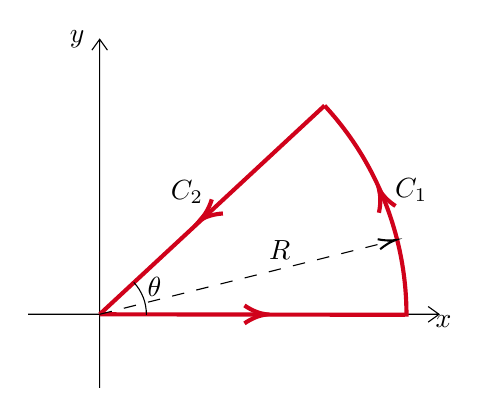
\begin{tikzpicture}[x=0.75pt,y=0.75pt,yscale=-0.75,xscale=0.75]
	%uncomment if require: \path (0,300); %set diagram left start at 0, and has height of 300
	
	%Shape: Axis 2D [id:dp9128522066257279] 
	\draw  (198,215.17) -- (461.9,215.17)(243.9,38.49) -- (243.9,262.49) (454.9,210.17) -- (461.9,215.17) -- (454.9,220.17) (238.9,45.49) -- (243.9,38.49) -- (248.9,45.49)  ;
	%Straight Lines [id:da5403715550088912] 
	\draw [color={rgb, 255:red, 208; green, 2; blue, 27 }  ,draw opacity=1 ][line width=1.5]    (243.9,215.17) -- (439.9,215.49) ;
	%Shape: Arc [id:dp48810296283958254] 
	\draw  [draw opacity=0][line width=1.5]  (388.36,81.11) .. controls (406.05,100.2) and (420.24,123.13) .. (429.51,149.22) .. controls (437.44,171.53) and (441.11,194.31) .. (440.97,216.68) -- (243.9,215.17) -- cycle ; \draw  [color={rgb, 255:red, 208; green, 2; blue, 27 }  ,draw opacity=1 ][line width=1.5]  (388.36,81.11) .. controls (406.05,100.2) and (420.24,123.13) .. (429.51,149.22) .. controls (437.44,171.53) and (441.11,194.31) .. (440.97,216.68) ;
	%Straight Lines [id:da785539995442484] 
	\draw [color={rgb, 255:red, 208; green, 2; blue, 27 }  ,draw opacity=1 ][line width=1.5]    (388.36,81.11) -- (243.9,215.17) ;
	\draw  [color={rgb, 255:red, 208; green, 2; blue, 27 }  ,draw opacity=1 ][line width=1.5]  (336.9,209.49) .. controls (341.6,212.69) and (346.3,214.61) .. (351,215.25) .. controls (346.3,215.88) and (341.6,217.8) .. (336.9,221) ;
	\draw  [color={rgb, 255:red, 208; green, 2; blue, 27 }  ,draw opacity=1 ][line width=1.5]  (423.27,149.94) .. controls (424.47,144.38) and (424.48,139.31) .. (423.29,134.71) .. controls (425.65,138.83) and (429.2,142.46) .. (433.94,145.61) ;
	\draw  [color={rgb, 255:red, 208; green, 2; blue, 27 }  ,draw opacity=1 ][line width=1.5]  (323.05,150.4) .. controls (317.38,150.79) and (312.5,152.2) .. (308.42,154.61) .. controls (311.71,151.2) and (314.21,146.78) .. (315.92,141.36) ;
	%Straight Lines [id:da20407447230286557] 
	\draw  [dash pattern={on 4.5pt off 4.5pt}]  (243.9,215.17) -- (431.96,167.98) ;
	\draw [shift={(433.9,167.49)}, rotate = 525.9100000000001] [color={rgb, 255:red, 0; green, 0; blue, 0 }  ][line width=0.75]    (10.93,-3.29) .. controls (6.95,-1.4) and (3.31,-0.3) .. (0,0) .. controls (3.31,0.3) and (6.95,1.4) .. (10.93,3.29)   ;
	%Shape: Arc [id:dp03335176702458664] 
	\draw  [draw opacity=0] (265.8,194.65) .. controls (271.14,200.34) and (273.98,207.86) .. (273.9,215.49) -- (243.9,215.17) -- cycle ; \draw   (265.8,194.65) .. controls (271.14,200.34) and (273.98,207.86) .. (273.9,215.49) ;
	
	% Text Node
	\draw (432,126.4) node [anchor=north west][inner sep=0.75pt]    {$C_{1}$};
	% Text Node
	\draw (288,127.4) node [anchor=north west][inner sep=0.75pt]    {$C_{2}$};
	% Text Node
	\draw (351,166.4) node [anchor=north west][inner sep=0.75pt]    {$R$};
	% Text Node
	\draw (273,189.4) node [anchor=north west][inner sep=0.75pt]    {$\theta $};
	% Text Node
	\draw (458,214.4) node [anchor=north west][inner sep=0.75pt]    {$x$};
	% Text Node
	\draw (223,31.4) node [anchor=north west][inner sep=0.75pt]    {$y$};
	
	
	\end{tikzpicture}
	
\end{figure}

Let $p=|p|\mathrm{e}^{\mathrm{i}\varphi}$, we have  
\begin{align*}
\int_{C_1}\mathrm{e}^{-px^2}\mathrm{d}x&=\lim_{R\to\infty}\int_0^\theta\mathrm{e}^{-|p|R^2\mathrm{e}^{\mathrm{i}(2\alpha+\varphi)}}\mathrm{i}R\mathrm{e}^{\mathrm{i}\alpha}\mathrm{d}\alpha\\
&\le \max\left|\mathrm{e}^{-|p|R^2\mathrm{e}^{\mathrm{i}(2\alpha+\varphi)}}R\right|\cdot\theta=0
\end{align*}
if $\text{Re}(\mathrm{e}^{\mathrm{i}(2\alpha+\varphi)})>0$. Thus, we choose $\theta=-\varphi/2$, and 
\begin{equation*}
\int_{C_2}\mathrm{e}^{-px^2}\mathrm{d}x=-\lim_{R\to\infty}\int_0^\infty\mathrm{e}^{-|p|R^2}\mathrm{e}^{\mathrm{i}\theta}\mathrm{d}R=-\mathrm{e}^{\mathrm{i}\theta}\frac{1}{2}\sqrt{\frac{\pi}{|p|}}=-\frac{1}{2}\sqrt{\frac{\pi}{|p|\mathrm{e}^{\mathrm{i}\varphi}}}=-\frac{1}{2}\sqrt{\frac{\pi}{p}}
\end{equation*}
Therefore, we have 
\begin{equation*}
\int_{-\infty}^{\infty}\mathrm{e}^{-px^2+c}\mathrm{d}x=\mathrm{e}^c\sqrt{\frac{\pi}{p}}
\end{equation*}

\subsection{Exercise 8.26}
	As 
	\begin{align*}
	\int_{-\infty}^\infty\varphi_m^*(x)\varphi_n(x)\mathrm{d}x&=\int_{-\infty}^\infty\frac{\sin^2\frac{x}{2}}{\pi^2 x^2}\mathrm{e}^{\mathrm{i}(n-m)x}\mathrm{d}x\\
	&=\frac{1}{2\pi}\delta_{mn}
	\end{align*}
	The basis $\{\varphi_n,n\in\mathbb Z\}$ is orthorgonal and complete. Thus the coefficients are 
	\begin{equation*}
	\begin{aligned}
	a_n&=2\pi\int_{-\infty}^\infty\frac{1}{1+x^2}\frac{\sin\frac{x}{2}}{\pi x}\mathrm{e}^{-\mathrm{i}nx}\mathrm{d}x=2\times2\pi\mathrm{i}\left(-\frac{\mathrm{i}}{2}\mathrm{e}^n\sinh\frac{1}{2}+\frac{\mathrm{i}}{2}\mathrm{e}^{-n}\sinh\frac{1}{2}\right)\\
	&=4\pi\sinh\frac{1}{2}\sinh \!n
	\end{aligned}
	\end{equation*}
	
\subsection{Exercise 8.27}

\subsection{Exercise 8.28}
We know:
\begin{equation*}
\begin{aligned}
H(x,y)=
\begin{cases}
1,x\geq 0,y \geq 0\\
0, \text{Otherwise}
\end{cases}
\end{aligned}
\end{equation*}

So:
\begin{equation*}
\begin{aligned}
\langle H_{,x,y}|\varphi\rangle&=-\langle H_{,x}|\varphi_{,y}\rangle=\langle H|\varphi_{,x,y}\rangle=\int_{\mathbb{R}^2}H(x,y)\frac{\pa \varphi}{\pa x \pa y} \di x \di y\\
&=\int_{0}^{\infty}\int_{0}^{\infty}\frac{\pa ^2 \varphi}{\pa x \pa y}\di x\di y =\int_{0}^{\infty}\left.\frac{\pa\varphi}{\pa x}\right|^{y=\infty}_{y=0}\di x \di y=-\int_{0}^{\infty}\frac{\pa \varphi}{\pa x }(x,0)\di x =\varphi(0,0)\\
&=\int_{\mathbb{R}^{2}} \delta(x, y) \varphi(x, y) \di  x \di y=\langle\delta(x, y) \mid \varphi\rangle \quad \Rightarrow \quad \frac{\partial^{2} H}{\partial x \partial y}=\delta(x, y)
\end{aligned}
\end{equation*}

\subsection{Exercise 8.29}
\begin{equation*}
\begin{aligned}
&F(x)=x^{2}-5 x+6 \quad F^{\prime}(x)=2 x-5 \\
\Rightarrow &\delta(F(x))=\sum_{i=1}^{m} \frac{\delta\left(x-a_{i}\right)}{\left|F^{\prime}\left(a_{i}\right)\right|}=\delta(x-2)+\delta(x-3)
\end{aligned}
\end{equation*}

\subsection{Exercise 8.30}
Suppose $F$ has isolated zeros $a_i$ with multiplicity $n$, so:
\begin{equation*}
\begin{aligned}
\int_{-\infty}^{+\infty} \delta(F(x)) f(x)&=\sum_{i} \int_{a_{i}-\varepsilon}^{a_{i}+\varepsilon} \delta\left(0+\ldots 0+\frac{f^{(n)}\left(a_{i}\right)}{n !}\left(x-a_{i}\right)^{n}\right) f(x) \di x \\
&=\sum_{i} \int_{-\varepsilon}^{+\varepsilon} \delta(y) f\left(\left(\frac{y}{c}\right)^{\frac{1}{n}}+a_{i}\right) \frac{1}{n c^{1/n} y^{1-1/n}} \di y \\
&=\sum_{i} \frac{f\left(a_{i}\right)}{n \cdot\left|\frac{f^{(n)}(a_i) }{n !}\right|\left(x-a_{i}\right)^{1-1/n} }
\end{aligned}
\end{equation*}

\subsection{Exercise 8.31}
	What we want to prove is:
		\begin{equation*}
		\begin{aligned}
			\langle \delta |\varphi\rangle=\varphi(0)
		\end{aligned}
		\end{equation*}
		
	For the first distribution, we have:
		\begin{equation*}
		\begin{aligned}
			\lim _{l \rightarrow 0}\left\langle\left.\frac{1}{l} \operatorname{rect} \frac{x}{l}\right|\varphi(x)\right\rangle=&\lim_{l\to 0}\int_{-\infty}^{\infty}\frac{1}{l}\operatorname{rect}\frac{x}{l}\varphi(x)\\
			\xlongequal[]{y=x/l}&\lim_{l\to 0}\int_{-\infty}^{\infty}\operatorname{rect}y\varphi(ly)\di y\\
			=&\lim_{l\to 0}\int_{-\frac{1}{2}}^{\frac{1}{2}}\varphi(lx)\di x\\
			=&\int_{-\frac{1}{2}}^{\frac{1}{2}}\lim_{l\to 0}\varphi(lx)\di x\\
			=&\int_{-\frac{1}{2}}^{\frac{1}{2}}\varphi(0)\di x\\
			=&\varphi(0)
		\end{aligned}
		\end{equation*}
		
	For the second distribution, we have:
		\begin{equation*}
		\begin{aligned}
			\lim _{K\rightarrow \infty}\left\langle\left.\frac{1}{\pi} \frac{\sin(Kx)}{x} \right|\varphi(x)\right\rangle\xlongequal[]{Kx\to y}&\lim _{K\rightarrow \infty}\frac{1}{\pi}\int_{-\infty}^{\infty}\frac{\sin y}{y}\varphi(\frac{y}{k})\di y\\
			=&\frac{1}{\pi}\int_{-\infty}^{\infty}\lim _{K\rightarrow \infty}\frac{\sin y}{y}\varphi(\frac{y}{k})\di y\\
			=&\frac{1}{\pi}\int_{-\infty}^{\infty}\frac{\sin y}{y}\varphi(0)\di y\\
			=&\frac{1}{\pi}\pi\varphi(0)\\
			=&\varphi(0)
		\end{aligned}
		\end{equation*}
	
	For the third distribution, we have:
		\begin{equation*}
		\begin{aligned}
			\lim _{\varepsilon\rightarrow 0}\left\langle\left.\frac{1}{\pi} \frac{\epsilon}{\epsilon^2+x^2} \right|\varphi(x)\right\rangle
			&=\int_{-\infty}^{\infty} \frac{\epsilon \varphi(x)}{x^{2}+\epsilon^{2}} \di x\\
			&=\int_{-\infty}^{\infty} \varphi(x) \di\left(\arctan \frac{x}{\epsilon}\right)\\
			&=\left.\left(\varphi(x)\arctan \frac{x}{\epsilon}\right)\right|_{-\infty} ^{\infty}-\int_{-\infty}^{\infty}\arctan \frac{x}{\epsilon}\varphi'\left( x\right) \\
			\Rightarrow \lim _{\epsilon \rightarrow 0^{+}} \int_{-\infty}^{\infty} \frac{\epsilon\varphi( x)}{x^{2}+\epsilon^{2}}\di x&=-\lim _{\delta_{1} \rightarrow 0^{+}} \lim _{\epsilon\to 0^{+}} \int_{-\infty}^{-\delta_{1}} \arctan \left(\frac{x}{\epsilon}\right) \varphi^{\prime}(x) \di x-
			\lim\limits_{\delta_{2} \rightarrow 0^{+}} \lim\limits_{\epsilon \rightarrow 0^{+}} \int_{\delta^{2}}^{+\infty} \arctan \left(\frac{x}{\epsilon}\right) \varphi^{\prime}(x) \di x \\
			&=\frac{\pi}{2} \int_{-\infty}^{0} \phi^{\prime}(x) \di x-\frac{\pi}{2} \int_{0}^{+\infty} \phi^{\prime}(x) \di x\\
			&=\frac{\pi}{2}\varphi(0)+\frac{\pi}{2} \varphi(0)=\pi \varphi(0)\\
			\Rightarrow \lim _{\varepsilon\rightarrow 0}\left\langle\left.\frac{1}{\pi} \frac{\epsilon}{\epsilon^2+x^2} \right|\varphi(x)\right\rangle&=\varphi(0)
		\end{aligned}
		\end{equation*}
		
	For $n$ dimensional case, we have:
		\begin{equation*}
		\begin{aligned}
		\langle\left(\delta\right)^n|&=\lim _{l \rightarrow 0}\left\langle\left(\frac{1}{l} \operatorname{rect} \frac{x_1}{l}\right)\left(\frac{1}{l} \operatorname{rect} \frac{x_2}{l}\right)\cdots\left(\frac{1}{l} \operatorname{rect} \frac{x_n}{l}\right)\right| \\
			\langle\left(\delta\right)^n|&=\lim _{K \rightarrow \infty}\left\langle\left(\frac{1}{\pi} \frac{\sin (K x_1)}{x_1}\right)\left(\frac{1}{\pi} \frac{\sin (K x_2)}{x_2}\right)\cdots\left(\frac{1}{\pi} \frac{\sin (K x_n)}{x_n}\right)\right|\\
			\langle\left(\delta\right)^n|&=\lim _{\epsilon \rightarrow 0}\left\langle\left(\frac{1}{\pi} \frac{\epsilon}{\epsilon^{2}+x_1^{2}}\right)\left(\frac{1}{\pi} \frac{\epsilon}{\epsilon^{2}+x_2^{2}}\right)\cdots \left(\frac{1}{\pi} \frac{\epsilon}{\epsilon^{2}+x_n^{2}}\right)\right|
		\end{aligned}
		\end{equation*}
		
	\subsection{Exercise 8.32}
		We have $f(r)=\frac{\delta(r-a)}{r}$, so:
			\begin{equation*}
			\begin{aligned}
				\tilde{f}(\vec{k}) &=\frac{1}{(2 \pi)^{3 / 2}} \int f(r) \me^{-\mi k r \cos \theta} \sin \theta r^{2} \di r \di \theta \di \phi=\frac{1}{\sqrt{2 \pi}} \iint \frac{\delta(r-a)}{r} r^{2} \me^{-\mi k r \cos \theta} \sin \theta \di r \di \theta \\
				&=\frac{1}{\sqrt{2 \pi}} \int_{0}^{\pi} a \me^{-\mi k a \cos \theta} \sin \theta \di \theta=\frac{1}{\sqrt{2 \pi}} \frac{1}{k} \int_{\cos \theta=-1}^{\cos \theta=1} \me^{-\mi k a \cos \theta} \di(a k \cos \theta) \\
				&=\sqrt{\frac{2}{\pi}} \frac{1}{k} \sin a k
			\end{aligned}
			\end{equation*}
		
	\subsection{Exercise 8.33}
		We know $\langle \tilde{f'}|=\langle\mi \omega \tilde{f}|$, So:
			\begin{equation*}
			\begin{aligned}
				\langle \widetilde{\mathcal{D}_{\alpha}f'}|=\langle\left(\mi \omega_1 \right)\left(\mi \omega_2 \right)\cdots \left(\mi \omega_n \right)\tilde{f}|
			\end{aligned}
			\end{equation*}
			
	\subsection{Exercise 8.34}
		\begin{equation*}
		\begin{aligned}
			\langle\tilde{f}|\tilde{\varphi}\rangle=\langle f|\tilde{\tilde{\varphi}}\rangle=\langle f|\varphi\rangle
		\end{aligned}
		\end{equation*}
		
	\subsection{Exercise 8.35}
		\begin{equation*}
		\begin{aligned}
			I(r)=\frac{1}{\mi} \frac{\partial}{\partial r}\underbrace{\int_{-\infty}^{\infty} F(p, r) \di p}_{J(\rho,r)}
		\end{aligned}
		\end{equation*}
		
	So we know that:
		\begin{equation*}
		\begin{aligned}
			\lim _{R \rightarrow \infty}\left(\int_{-\infty}^{\infty}+\int_{C_{\epsilon}}+\int_{C_{R_{1}}}+\int_{C_{R_{2}}}+\int_{l_{1}}+(-1) \int_{l_{2}}\right) \frac{\me^{\mi \rho r}}{\sqrt{\rho^{2}+m^{2}}}\di \rho=0
		\end{aligned}
		\end{equation*}
		
	According to Jordan's lemma:
		\begin{equation*}
		\begin{aligned}
			\int_{C_{R_{1}}} F(\rho, r) \di 
			 \rho=\int_{C_{R_{2}}} F(\rho, r) \di \rho=0
		\end{aligned}
		\end{equation*}
		
	We also know that the integral vanishes on $C_{\epsilon}$, so:
		\begin{equation*}
		\begin{aligned}
		\Rightarrow  J(\rho, r) &=\lim _{R \rightarrow \infty}\left(\int_{l_{2}}-\int_{l_{1}}\right) F\left(\rho, r\right) \di \rho=2 \int_{\mi m}^{\mi \infty} \frac{\me^{\mi \rho r}}{\sqrt{\rho^{2}+m^{2}}} \di \rho=2 \int_{m}^{\infty} \frac{\me^{-r \rho}}{\mi \sqrt{\rho^{2}-m^{2}}}\mi \di \rho \\
		&=2 \int_{m}^{\infty} \frac{\me^{-\rho r}}{\sqrt{\rho^{2}-m^{2}}} \di \rho \\
		\Rightarrow I_{(r)} & \sim \frac{\partial}{\partial r} J\left(\rho,r\right) \sim \int_{m}^{\infty} \frac{\rho \me^{-\rho r}}{\sqrt{\rho^{2}-m^{2}}} \di \rho \sim K_{1}(m r)
		\end{aligned}
		\end{equation*}
		\subsection{Exercise 8.36}
		As we have $f_\epsilon(\rho)=f(\rho)\mathrm{e}^{-\epsilon|\rho|}$, noting that $|f(\rho)|\to 1$ when $|\rho|\to\infty$, we find that $f_\epsilon(\rho)$ 
		satisfies the Jordan Lemma in the upper plane. Thus we explicitly have 
		\begin{align*}
		&\;\;\;\;\lim_{\epsilon\to 0^+}\int_{\mathbb R}f(\rho)\mathrm{e}^{-\epsilon|\rho|}\mathrm{e}^{\mathrm{i}\rho r}\mathrm{d}\rho,\;\;f(\rho)=\frac{\rho}{\sqrt{\rho^2+m^2}}\\
		&=\lim_{\epsilon\to 0^+}\int_m^\infty\frac{\rho}{\sqrt{\rho^2+m^2}}\mathrm{e}^{-\rho(\epsilon+r)}\mathrm{d}\rho\\
		&=\lim_{\epsilon\to 0^+} K_1\big[m(\epsilon+r)\big]\\
		&=K_1(mr)
		\end{align*}
		which is in agreement with Eq.(8.115). 
		
		\subsection{Exercise 8.37}
		Noting that 
		\begin{equation*}
		g_\epsilon(x)=\theta(x-1/\epsilon)-\theta(x-1-1/\epsilon)
		\end{equation*}
		Thus 
		\begin{align*}
		\int_{\mathbb R}\lim_{\epsilon\to 0}g_\epsilon(x)\mathrm{d}x&=\int_{\mathbb R}\lim_{\epsilon\to 0}\frac{\theta(x-1/\epsilon)-\theta(x-1-1/\epsilon)}{1}\mathrm{d}x\\
		&=\int_{\mathbb R}\lim_{\epsilon\to 0}\frac{\theta(\epsilon x-1)-\theta(\epsilon x-1-\epsilon)}{\epsilon}\mathrm{d}(\epsilon x-1)\\
		&=\int_{\mathbb R}\theta'(x)\mathrm{d}x\\
		&=\int_{\mathbb R}\delta(x)\mathrm{d}x=1=\lim_{\epsilon\to 0}\int_\mathbb R g_\epsilon(x)\mathrm{d}x
		\end{align*}
		
		
		\subsection{Exercise 8.38}
		\begin{align*}
		\tilde{\theta}(\omega)&=\lim_{\epsilon\to 0^+}\int_{-\infty}^\infty\theta(x)\mathrm{e}^{-\mathrm{i}(\omega-\mathrm{i}\epsilon)x}\mathrm{d}x\\
		&=\lim_{\epsilon\to 0^+}\int_0^\infty\mathrm{e}^{-\mathrm{i}(\omega-\mathrm{i}\epsilon)x}\mathrm{d}x\\
		&=\lim_{\epsilon\to 0^+}\frac{1}{\mathrm{i}(\omega-\mathrm{i}\epsilon)}\\
		&=\frac{1}{\mathrm{i}\omega}+\pi\delta(\omega)
		\end{align*}
		\subsection{Exercise 8.39}
		Single particle partition function 
		\begin{equation}
		z=\int_0^\infty w(\varepsilon)\mathrm{e}^{-\beta\varepsilon}\mathrm{d}\varepsilon=2\pi V\left(\frac{2m}{\beta h^2}\right)^{3/2}\Gamma\left(\frac 32\right)=V\left(\frac{2\pi m}{\beta h^2}\right)^{3/2}
		\end{equation}
		The partition function of $N$ identical particle is then given by 
		\begin{equation*}
		Z=\frac{z^N}{N!}=\frac{V^N}{N!}\left(\frac{2\pi m}{\beta h^2}\right)^{3N/2}
		\end{equation*}
		Then we have
		\begin{align*}
		g(E)&=\frac{1}{2\pi\mathrm{i}}\int_{\beta'-\mathrm{i}\infty}^{\beta'+\mathrm{i}\infty}\frac{V^N}{N!}\left(\frac{2\pi m}{\beta h^2}\right)^{3N/2}\mathrm{e}^{\beta E}\mathrm{d}\beta \\
		&=\frac{V^N}{N!}\left(\frac{2\pi m}{h^2}\right)^{3N/2}\left.\left(\frac{\mathrm{d}}{\mathrm{d}\beta}\right)^{3N/2-1}\mathrm{e}^{\beta E}\right|_{\beta=0}\\
		&\sim \frac{V^N}{N!}\left(\frac{2\pi m}{h^2}\right)^{3N/2}\frac{E^{3N/2}}{(3N/2)!}
		\end{align*}
		
		\subsection{Exercise 8.40}
		For a single harmonic oscillator, 
		\begin{equation*}
		Z(\beta)=\frac{1}{2\sinh(\beta\hbar\omega/2)}
		\end{equation*}
		Thus the state density is given by 
		\begin{align*}
		w(\varepsilon)&=\frac{1}{2\pi\mathrm{i}}\int_{\beta'-\mathrm{i}\infty}^{\beta'+\mathrm{i}\infty}\frac{\mathrm{e}^{\beta E}}{2\sinh(\beta\hbar\omega/2)}\mathrm{d}\beta\\
		&=\frac{1}{2\pi\mathrm{i}}\frac{2}{\hbar\omega}\int_{\beta'-\mathrm{i}\infty}^{\beta'+\mathrm{i}\infty}\frac{\mathrm{e}^{2\beta E/\hbar\omega}}{\mathrm{e}^\beta-\mathrm{e}^{-\beta}}\\
		&=\frac{2}{\hbar\omega}\sum_{n\in\mathbb Z}\lim_{\beta\to n\pi\mathrm{i}}(\beta-n\pi\mathrm{i})\frac{\mathrm{e}^{\beta(2E/\hbar\omega+1)}}{\mathrm{e}^{2\beta}-1}\\
		&=\frac{1}{\hbar\omega}\sum_{n\in\mathbb Z}\exp\left[\mathrm{i}n\pi\left(\frac{2E}{\hbar\omega}+1\right)\right]
		\end{align*}
		Noting that 
		\begin{equation*}
		\sum_{k\in\mathbb Z}\mathrm{e}^{\mathrm{i}k(x-a)}=\frac{1}{2\pi}\delta(x-a),\;\;x-a\in(-\pi,\pi)
		\end{equation*}
		we have 
		\begin{equation*}
		w(\varepsilon)=\frac{1}{\hbar \omega}2\pi\sum_{k\in\mathbb Z}\delta\left[\pi\left(\frac{2E}{\hbar\omega}+1\right)+2k\pi\right]\overset{E>0}{=}\sum_{k\in\mathbb Z_0^+}\delta\left[E-\left(k+\frac{1}{2}\right)\hbar\omega\right]
		\end{equation*}
		
		\subsection{Exercise 8.41}
		\begin{align*}
		\int_0^\infty f^{(n)}(t)\mathrm{e}^{-pt}\mathrm{d}t&=f^{(n-1)}(t)\mathrm{e}^{-pt}\big|_0^\infty+p\int_0^\infty f^{(n-1)}(t)\mathrm{e}^{-pt}\mathrm{d}t\\
		&\cdots\\
		&=p^n\bar f(p)-\sum_{j=0}^{n-1}p^j f^{(n-1-j)}(0)
		\end{align*}
		
		\subsection{Exercise 8.42}
		\begin{equation*}
		f(t-t_0)\fallingdotseq \int_0^\infty f(t-t_0)\mathrm{e}^{-p(t-t_0)}\mathrm{e}^{-pt_0}\mathrm{d}(t-t_0)=\mathrm{e}^{-pt_0}\bar f(p)
		\end{equation*}
		
		\subsection{Exercise 8.43}
		\begin{equation*}
		\mathrm{e}^{-\lambda t}f(t)\fallingdotseq\int_0^\infty\mathrm{e}^{-\lambda t}f(t)\mathrm{e}^{-pt}\mathrm{d}t=\bar f(p+\lambda)
		\end{equation*}
		
		\subsection{Exercise 8.44}
		\subsection{Exercise 8.45}
		If $\lambda\ne\mathbb Z^+_0$, then the Taylor expansion of $(1-p)^\lambda$ has infinite terms, and so does its inverse Laplace transformation. 
		Hence $f(t)$ is not a polynomial. If $\lambda\in\mathbb Z^+_0$, then 
		\begin{equation*}
		f(t)=\frac{1}{2\pi\mathrm{i}}\int_{\beta'-\mathrm{i}\infty}^{\beta'+\mathrm{i}\infty}\frac{(p-1)^\lambda}{p^{\lambda+1}}\mathrm{e}^{pt}\mathrm{d}p=\lim_{p\to 0}\frac{\mathrm{d}^\lambda}{\mathrm{d}p^\lambda}(1-p)^\lambda\mathrm{e}^{pt}
		\end{equation*}
		which is obviously a polynomial of $t$, reads 
		\begin{equation*}
		f(t)=\sum_{k=0}^\lambda t^{k}\left.\frac{\mathrm{d}^{\lambda-k}}{\mathrm{d}p^{\lambda-k}}(1-p)^\lambda\right|_{p=0}
		\end{equation*}
		\subsection{Exercise 8.46}
		Take the derivative on both sides of the equation, we have 
		\begin{equation*}
		R\dot J(t)+\frac{1}{C}J(t)=\omega E_0\cos\omega t
		\end{equation*}
		Then apply the Laplace transformation: 
		\begin{equation*}
		Rp\bar J+\frac{1}{C}\bar J=\omega E_0\overline{\cos\omega t}\;\;\Rightarrow\;\;\bar J=\frac{\omega E_0\overline{\cos\omega t}}{R(p+1/CR)}
		\end{equation*}
		Noting that 
		\begin{equation*}
		\frac{1}{p+1/CR}\risingdotseq\mathrm{e}^{-t/CR}
		\end{equation*}
		and using the convolution property of the Laplace transformation, we have 
		\begin{align*}
		J(t)&=\int_{-\infty}^\infty E_0\cos\omega t'\mathrm{e}^{-(t-t')/CR}\theta(t')\theta(t-t')\mathrm{d}t'\\
		&=\int_0^t\frac{\omega E_0}{2R}\mathrm{e}^{-\frac{t}{CR}}\left[\mathrm{e}^{\left(\frac{1}{CR}+\mathrm{i}\omega\right)t'}+\mathrm{e}^{\left(\frac{1}{CR}-\mathrm{i}\omega\right)t'}\right]\mathrm{d}t'\\
		&=\frac{\omega E_0}{R}\frac{\omega\sin\omega t+\dfrac{1}{CR}\cos\omega t}{\omega^2+\dfrac{1}{(CR)^2}}-\frac{1}{CR}\mathrm{e}^{-\frac{t}{CR}}
		\end{align*}
		
		\subsection{Exercise 8.47}
		Let 
		\begin{equation*}
		f(t)=\sum_{n=2}^\infty a_n t^n+a_1 t+a_0
		\end{equation*}
		Insert the expression in the Hermite equation, we have 
		\begin{equation*}
		\sum_{n=2}^\infty\left[a_n n(n-1)t^{n-2}-2a_n nt^n+\lambda a_n t^n\right]-2a_1 t+\lambda a_1 t+a_0=0
		\end{equation*}
		If we want $f(t)$ to be a polynomial, we must cut off this series at some $n\in\mathbb Z^+$. Thus: 
		\begin{equation*}
		-2a_1+\lambda a_1=0\;\;\Rightarrow\;\;\lambda=2
		\end{equation*}
		or for $n\ge 2$, 
		\begin{equation*}
		a_{n+2}(n+1)(n+2)=2n a_n-\lambda a_n=0\;\;\Rightarrow\;\;\lambda=2n
		\end{equation*}
		Therefore we have $\lambda=2n$, $n\in\mathbb Z^+$. 
	
	
\section{Group Representations, Differential Equations and Special Functions}
\subsection{Exercise 9.1}
For $m=0$, 
\begin{equation*}
\frac{1}{\rho}\frac{\mathrm{d}}{\mathrm{d}\rho}\left(\rho\frac{\mathrm{d}R}{\mathrm{d}\rho}\right)=0\;\;\Rightarrow\;\;\frac{\mathrm{d}R}{\mathrm{d}\rho}=\frac{F}{\rho}\;\;\Rightarrow\;\;R(\rho)=E+F\ln\rho
\end{equation*}
For $m\in\mathbb Z^+$, then let $\rho=\mathrm{e}^x$, we have 
\begin{equation*}
\frac{\mathrm{d}}{\mathrm{d}\rho}=\frac{\mathrm{d}x}{\mathrm{d}\rho}\frac{\mathrm{d}}{\mathrm{d}x}=\frac{1}{\rho}\frac{\mathrm{d}}{\mathrm{d}x},\;\;\frac{\mathrm{d}^2}{\mathrm{d}\rho^2}=\frac{1}{\rho}\frac{\mathrm{d}}{\mathrm{d}x}\left(\mathrm{e}^{-x}\frac{\mathrm{d}}{\mathrm{d}x}\right)=\frac{1}{\rho^2}\frac{\mathrm{d}^2}{\mathrm{d}x^2}-\frac{1}{\rho^2}\frac{\mathrm{d}}{\mathrm{d}x}
\end{equation*}
Thus the equation becomes
\begin{equation*}
\frac{1}{\rho^2}\left(\frac{\mathrm{d}^2R}{\mathrm{d}x^2}-\frac{\mathrm{d}R}{\mathrm{d}x}\right)+\frac{1}{\rho^2}\frac{\mathrm{d}R}{\mathrm{d}x}-\frac{m^2}{\rho^2}R=0\;\;\Rightarrow\;\;\frac{\mathrm{d}^2R}{\mathrm{d}x^2}=m^2R
\end{equation*}
which has solutions 
\begin{equation*}
R=E\mathrm{e}^{mx}+F\mathrm{e}^{-mx}
\end{equation*}
Therefore, we have 
\begin{equation*}
R(\rho)=E\mathrm{e}^{m\ln\rho}+F\mathrm{e}^{-m\ln\rho}=E\rho^m+F\rho^{-m}
\end{equation*}

\subsection{Exercise 9.2}
For the wave equation, after the seperation of variables $u(t,\mathbf x)=T(t)v(\mathbf x)$, we have 
\begin{equation*}
\ddot Tv-a^2T\Delta v=0\;\;\Rightarrow\;\;\frac{\ddot T}{T}=a^2\frac{\Delta v}{v}=-k^2a^2
\end{equation*}
The equation of $T$ then reads 
\begin{equation*}
\ddot T+k^2a^2 T=0\;\;\Rightarrow\;\;T(t)=A\cos(akt)+B\sin(akt)
\end{equation*}
For the transport equation, after the seperation of variables $u(t,\mathbf x)=T(t)v(\mathbf x)$, we have
\begin{equation*}
\dot Tv-a^2T\Delta v=0\;\;\Rightarrow\;\;\frac{\dot T}{T}=a^2\frac{\Delta v}{v}=-k^2a^2
\end{equation*}
The equation of $T$ then reads 
\begin{equation*}
\dot T=-k^2a^2 T\;\;\Rightarrow\;\;T(t)=A\mathrm{e}^{-k^2a^2 t}
\end{equation*}
Noting that if $k^2<0$, then $T(t)$ will diverge at $r\to\infty$ or $r\to 0$ unless $T(t)\equiv 0$ for the two cases above. 
\subsection{Exercise 9.3}
If $\nu^2<0$, then $Z$ will diverge at $z\to\infty$ or $z\to 0$ unless $Z\equiv 0$, hence the only possible solution for $\nu^2<0$ is trivial. 
Therefore we let $\nu^2>0$. 
\subsection{Exercise 9.4}
\subsubsection*{9.4.1}
The Taylor expansion of $F(\bar x,\bar y,\bar p)$ around $(x,y,p)$ is 
\begin{equation*}
F(\bar x,\bar y,\bar p)=F(x+\epsilon\xi,y+\epsilon\eta, p+\epsilon\zeta)=\sum_{n=0}^{\infty}\frac{1}{n!}\left(\epsilon\xi\frac{\partial}{\partial x}+\epsilon\eta\frac{\partial}{\partial y}+\epsilon\zeta\frac{\partial}{\partial p}\right)^nF(x,y,p)=\mathrm{e}^{\epsilon X}F(x,y,p)
\end{equation*}
where we have defined the prolonged operator 
\begin{equation*}
X=\xi\frac{\partial}{\partial x}+\eta\frac{\partial}{\partial y}+\zeta\frac{\partial}{\partial z}
\end{equation*}
\subsubsection*{9.4.2}
Since $F(x,y,p)=F(\bar x,\bar y,\bar p)=0$, we have 
\begin{equation*}
\mathrm{e}^{\epsilon X}F(x,y,p)=0=(1+\epsilon X+\mathcal O(\epsilon^2))F(x,y,p)\;\;\Rightarrow\;\;XF(x,y,p)=0
\end{equation*}
Thus we have the determing equation: 
\begin{equation*}
\xi\frac{\partial F}{\partial x}+\eta\frac{\partial F}{\partial y}+\zeta\frac{\partial F}{\partial p}=0
\end{equation*}
Since 
\begin{align*}
\bar p&=\frac{\mathrm{d}\bar y}{\mathrm{d}\bar x}=\frac{\mathrm{d}y+\epsilon\mathrm{d}\eta}{\mathrm{d}x+\epsilon\mathrm{d}\xi}\\
&=\frac{p+\epsilon(\eta_{,x}+\eta_{,y}p)}{1+\epsilon(\xi_{,x}+\xi_{,y}p)}\\
&=\big[p+\epsilon(\eta_{,x}+\eta_{,y}p)\big]\big[1-\epsilon(\xi_{,x}+\xi_{,y}p)+\mathcal O(\epsilon^2)\big]\\
&=p+\epsilon(\eta_{,x}+\eta_{,y}p-\xi_{,x}p-\xi_{,y}p^2)+\mathcal O(\epsilon^2)\\
&\overset{!}{=}p+\epsilon\zeta(x,y,p)
\end{align*}
Thus we have the first prolongation equation: 
\begin{equation*}
\zeta(x,y,p)=\eta_{,x}+(\eta_{,y}-\xi_{,x})p-\xi_{,y}p^2
\end{equation*}
\subsubsection*{9.4.3}
For the equation 
\begin{equation*}
y^2-\frac{y}{x}-\frac{\mathrm{d}y}{\mathrm{d}x}=0\;\;\Rightarrow\;\;F(x,y,p)=xy^2-y-xp=0
\end{equation*}
The determing equation reads 
\begin{equation*}
\xi(p-y^2)+\eta(1-2xy)+\zeta x=0
\end{equation*}
Applying the first prolongation equation and $p=y^2-y/x$, we have 
\begin{equation*}
\xi\left(-\frac{y}{x}\right)+\eta(1-2xy)+\eta_{,x}x+(\eta_{,y}-\xi_{,x})(xy^2-y)-\xi_{,y}\left(xy^4-2y^3+\frac{y^2}{x}\right)=0
\end{equation*}
\subsubsection*{9.4.4}
Assume 
\begin{equation*}
\begin{cases}
\xi=\xi_{00}+\xi_{01}x+\xi_{10}y\\
\eta=\eta_{00}+\eta_{01}x+\eta_{10}y
\end{cases}
\end{equation*}
we have 
\begin{align*}
&(\xi_{00}+\xi_{01}x+\xi_{10}y)\left(-\frac{y}{x}\right)+(\eta_{00}+\eta_{01}x+\eta_{10}y)(1-2xy)+\eta_{01}x\\
+{\;}&(\eta_{10}-\xi_{01})(xy^2-y)-\xi_{10}\left(xy^4-2y^3+\frac{y^2}{x}\right)=0
\end{align*}
If we want the above equation holds for arbitary $x$ and $y$, we have 
\begin{equation*}
\xi_{00}=\xi_{10}=\eta_{00}=2\eta_{01}=0,\;\;\eta_{10}+\xi_{01}=0
\end{equation*}
Therefore, we can set $\xi_{01}=1$ and $\eta_{10}=-1$, which gives $\xi=x$, $\eta=-y$ and $\zeta=-2p$, hence we have 
\begin{equation*}
X=x\frac{\partial}{\partial x}-y\frac{\partial}{\partial y}-2p\frac{\partial}{\partial p}
\end{equation*}
\subsubsection*{9.4.5}
If we let 
\begin{equation*}
\begin{pmatrix}
R\\S\\T
\end{pmatrix}=\begin{pmatrix}
xy\\\ln y\\x^2p
\end{pmatrix}
\end{equation*}
we have 
\begin{equation*}
X\begin{pmatrix}
R\\S\\T
\end{pmatrix}=\begin{pmatrix}
1-1\\-1\\2x^2p-2x^2p
\end{pmatrix}=\begin{pmatrix}
0\\-1\\0
\end{pmatrix}
\end{equation*}
Therefore this is indeed a solution, which implies that 
\begin{equation*}
x=R\mathrm{e}^{-S},\;\;y=\mathrm{e}^S,\;\;\frac{\mathrm{d}y}{\mathrm{d}x}=\frac{T}{R^2}\mathrm{e}^{2S}
\end{equation*}
then we see that 
\begin{equation*}
F(x,y,p)=xp+y-xy^2=\mathrm{e}^{S}\left(\frac{T}{R}+1-R\right)=0\;\;\Rightarrow\;\;T=-R+R^2
\end{equation*}
Moreover, as 
\begin{equation*}
\frac{\mathrm{d}S}{\mathrm{d}R}=\frac{\mathrm{d}\ln y/\mathrm{d}x}{\mathrm{d}(xy)/\mathrm{d}x}=\frac{p/y}{y+xp}=\frac{(T/R^2)\mathrm{e}^S}{\mathrm{e}^S+(T/R)\mathrm{e}^S}=\frac{-1/R+1}{1+R-1}=\frac{1}{R}-\frac{1}{R^2}
\end{equation*}
we have 
\begin{equation*}
y=\mathrm{e}^S=\mathrm{e}^{\ln R+\frac{1}{R}+C}=xy\mathrm{e}^{1/xy+C}\;\;\Rightarrow\;\;y=-\frac{1}{x(\ln x+C)}
\end{equation*}
where $C$ is a constant. 

\subsubsection*{9.4.6}
	We first find out $\eta^{(2)}$:
		\begin{equation*}
		\begin{aligned}
			\eta^{(2)}\left(x, y, y^{(1)}, y^{(2)}\right)&=D^{(1)} \eta^{(1)}-y^{(2)} D^{(0)} \xi\\
			&=\eta_{,x x}+\left(2 \eta_{,x y}-\xi_{,x x}\right) y^{\prime}+\left(\eta_{,y y}-2 \xi_{,x y}\right) y^{\prime 2}-\xi_{,y y} y^{\prime 3}+\left(\eta_{,y}-2 \xi_{,x}-3 \xi_{,y y^{\prime}}\right) y^{\prime \prime}
		\end{aligned}
		\end{equation*}
		
	Plug this and the expression of $\eta^{(1)}$ in, then the determining equation reads:
		\begin{equation*}
		\begin{aligned}
			&-\eta\left(\frac{y^{(1)^{2}}}{y^{2}}+2 y\right)+\left(\eta_{, x}+y^{(1)}\left(\eta_{, y}-\xi_{, x}\right)-y^{(1)^{2}} \xi,_{y}\right) \frac{2 y^{(1)}}{y}\\
			=&\left(\eta_{, x x}+y^{(1)}\left(2 \eta_{, x y}-\xi_{, x x}\right)+y^{(1)^{2}}\left(\eta_{, y y}-2 \xi_{, x y}\right)+\left(\frac{y^{(1)^{2}}}{y}-y^{2}\right)\left(\eta_{, y}-2 \xi_{, x}-3 y^{(1)} \xi_{, y}\right)-y^{(1)^{3}} \xi, y y\right)
		\end{aligned}
		\end{equation*}
		
	Comparing the coefficient of powers of $y^{(1)}$, we can get the equations:
		\begin{equation*}
			\begin{aligned}
			\xi_{y y}+\frac{1}{y} \xi_{y} &=0 \\
			\eta_{y y}-2 \xi_{x y}-\frac{1}{y} \eta_{y}+\frac{1}{y^{2}} \eta &=0 \\
			2 \eta_{x y}-\xi_{x x}+3 y^{2} \xi_{y}-\frac{2}{y} \eta_{x} &=0 \\
			\eta_{x x}-y^{2}\left(\eta_{y}-2 \xi_{x}\right)+2 y \eta &=0
			\end{aligned}
		\end{equation*}
		
	Solve the first equation and we have:
		\begin{equation*}
		\begin{aligned}
			\xi=A(x) \ln |y|+B(x)
		\end{aligned}
		\end{equation*}
	
	The second equation gives:
		\begin{equation*}
		\begin{aligned}
			\eta=A^{\prime}(x) y(\ln |y|)^{2}+C(x) y \ln |y|+D(x) y
		\end{aligned}
		\end{equation*}
		
	Plug these two equation into the third equation, we have:
		\begin{equation*}
		\begin{array}{c}
			3 A^{\prime \prime}(x) \ln |y|+3 A(x) y+2 C^{\prime}(x)-B^{\prime \prime}(x)=0\\
			\Rightarrow	A(x)=0,\quad B''(x)=2C'(x)
		\end{array}
		\end{equation*}
		
	Put them into last equation, we have:
		\begin{equation*}
		\begin{array}{c}
			C(x) y^{2} \ln |y|+C^{\prime \prime}(x) y \ln |y|+\left(2 B^{\prime}(x)-C(x)+D(x)\right) y^{2}+D^{\prime \prime}(x) y=0\\
			\Rightarrow C(x)=0, ~D(x)=2B'(x),~ D''(x)=0\\
			\Rightarrow B(x)=c_1+c_2x,\quad D(x)=-c_2\\
			\Rightarrow \xi=c_1+c_2x, \quad \eta =-2c_2y
		\end{array}
		\end{equation*}
	
	So that we can write the generator of this Lie group:
		\begin{equation*}
		\begin{aligned}
			X&=\xi\pa_x+\eta\pa_y\\
			&=(c_1+c_2x)\pa_x-2c_2y\pa_y\\
			&=c_1\pa_x+c_2(x\pa_x-2y\pa_y)
		\end{aligned}
		\end{equation*}
		
	\subsubsection*{9.4,7}
		We first figure out the coresponding Lie group element of this Lie algebra element. The given element can be written as:
			\begin{equation*}
			\begin{aligned}
				\hat{x}=\xi\pa_x+\eta \pa_y=0\pa_x+y\pa_y
			\end{aligned}
			\end{equation*}
		So:
			\begin{equation*}
			\begin{aligned}
				\eta^{(1)}&=D^{(0)}\eta-y^{1}D^{(0)}\xi\\
				&=(\pa_x+y^{(1)}\pa_y)\eta90=y^{(1)}\\
				\eta^{(2)}&=D^{(1)}\eta^{(1)}-y^{(2)}D^{(0)}\xi\\
				&=(\pa_x+y^{(1)}\pa_y+y^{(2)}\pa_{y^{(1)}})\eta^{1}-0=y^{(2)}
			\end{aligned}
			\end{equation*}
		Then the Lie group element looks like:
			\begin{equation*}
			\begin{aligned}
				X=y\pa_y+y^{(1)}\pa_{y^{(1)}}+y^{(2)}\pa_{y^{(2)}}
			\end{aligned}
			\end{equation*}
			
		Rewrite the equation:
			\begin{equation*}
			\begin{aligned}
				F(x,y,y^{(1)},y^{(2)})=y^{(2)}-\left(\frac{3}{x}-2x\right)y^{(1)}-4y\\
				\Rightarrow XF=y(-4)-y^{(1)}\left(\frac{3}{x}-2x\right)+y^{(2)}=F=0
			\end{aligned}
			\end{equation*}
		
	\subsubsection*{9.4.8}
		We have:
			\begin{equation*}
			\begin{aligned}
				R=x,\quad S=\ln (y)
			\end{aligned}
			\end{equation*}
			
		So that:
			\begin{equation*}
			\begin{aligned}
				\frac{\di S}{\di R}&=\frac{(1/y) \di y}{\di x}=\frac{y'}{y}=T\\
				\frac{\di T}{\di R}&=\frac{\di( y'/y)}{\di x}=\frac{y''y-y'^2}{y^2}=\frac{1}{y}\left[\left(\frac{3}{x}-2x\right)y'+4y\right]-T^2=\left(\frac{3}{R}-2R\right)T+4-T^2
			\end{aligned}
			\end{equation*}
			
		To solve the Riccati equation, we may use the power series, set
			\begin{equation*}
			\begin{aligned}
				T=\sum_{n=0}^{\infty}a_nR^n
			\end{aligned}
			\end{equation*}
			
		Then:
			\begin{equation*}
			\begin{aligned}
				\sum_{n=1}^{\infty}na_nR^{n-1}=\left(\frac{3}{R}-2R\right)\sum_{n=0}^{\infty}a_nR^n+4-\left(\sum_{n=0}^{\infty}a_nR^n\right)^2
			\end{aligned}
			\end{equation*}
		Comparing the first two coefficient:
			\begin{equation*}
			\begin{aligned}
				&a_0=0\\
				&a_1=-2
			\end{aligned}
			\end{equation*}
			
		Stop here and we can actually find that $T=-2R$ is already a solution. So we suppose the solutions are of the form:
			\begin{equation*}
			\begin{aligned}
				T=-2R+v
			\end{aligned}
			\end{equation*}
			
		Plug in, and we have:
			\begin{equation*}
			\begin{aligned}
				\frac{\di v}{\di R}=\left(\frac{3}{R}+2R\right)v-v^2
			\end{aligned}
			\end{equation*}
			
		It is actually a Bernoulli differential equation, so we just set $w=\frac{1}{v}$, and we can get:
			\begin{equation*}
			\begin{aligned}
				\frac{\di w}{\di R}&=1-\left( \frac{3}{R}+2R\right) w\\
				\Rightarrow w&=\frac{c_{1}}{R^{3}} \me^{-R^{2}}+\frac{1}{2 R}-\frac{1}{2 R^{3}}
			\end{aligned}
			\end{equation*}
			
		So the final solution is:
			\begin{equation*}
			\begin{aligned}
				y=\tilde{c}_{1} \me^{-x^{2}}+\tilde{c}_{2}\left(x^{2}-1\right)
			\end{aligned}
			\end{equation*}
\subsection{Exercise 9.5}
\subsubsection*{9.5.1}
By definition, we have $g((0,y),0)g((x,0),0)=g((x,y),0)$, i.e.,
\begin{equation*}
\mathrm{e}^{-\mathrm{i}yP_2}\mathrm{e}^{-\mathrm{i}xP_1}=\mathrm{e}^{-\mathrm{i}(xP_1+yP_2)}
\end{equation*}
Expanding the above equation gives 
\begin{equation*}
\left(1-\mathrm{i}yP_2-\frac{1}{2}y^2P_2^2\right)\left(1-\mathrm{i}xP_1-\frac{1}{2}x^2P_1^2\right)=1-\mathrm{i}xP_1-\mathrm{i}yP_2-\frac{1}{2}(xP_1+yP_2)^2
\end{equation*}
which implies 
\begin{equation*}
-xyP_1P_2=-\frac{1}{2}xy(P_1P_2+P_2P_1)\;\;\Rightarrow\;\;P_1P_2=P_2P_1\;\;\Rightarrow\;\;\big[P_1,P_2\big]=0
\end{equation*}

To deive $[J,P_{1}]$, we consider $g(0,\varphi)g((x,0),0)=g(R(\varphi)(x,0),\varphi)\simeq g(((1-\varphi^2/2)x,\varphi x),\varphi)$, i.e., 
\begin{equation*}
\mathrm{e}^{-\mathrm{i}\varphi J}\mathrm{e}^{-\mathrm{i}xP_1}=\mathrm{e}^{-\mathrm{i}\left[\left(1-\frac{1}{2}\varphi^2\right)xP_1+\varphi xP_2+\varphi J\right]}
\end{equation*}
Expand the above eqaution: 
\begin{align*}
\left(1-\mathrm{i}\varphi J-\frac{1}{2}\varphi^2 J^2\right)\left(1-\mathrm{i}xP_1-\frac{1}{2}x^2P_1^2\right)={}&1-\mathrm{i}\left(1-\frac{1}{2}\varphi^2\right)xP_1-\mathrm{i}\varphi xP_2-\mathrm{i}\varphi J\\
-\;&\frac{1}{2}\left[\left(1-\frac{1}{2}\varphi^2\right)xP_1+\varphi xP_2+\varphi J\right]^2
\end{align*}
which implies 
\begin{equation*}
-x\varphi JP_1=-\mathrm{i}x\varphi P_2-x\varphi P_1J\;\;\Rightarrow\;\;\big[J,P_1\big]=\mathrm{i}P_2
\end{equation*}
Simiarly, by expanding $g(0,\varphi)g((0,y),0)$, we can derive 
\begin{equation*}
\big[J,P_2\big]=-\mathrm{i}P_1
\end{equation*}

\subsubsection*{9.5.2}
By definition we have 
\begin{equation*}
\mathrm{e}^{-\mathrm{i}\theta J}\mathrm{e}^{-\mathrm{i}\mathbf P\cdot\mathbf x}\mathrm{e}^{\mathrm{i}\theta J}=g(0,\theta)g(\mathbf x,0)g(0,-\theta)=g(0,\theta)g(\mathbf x,-\theta)=g(R(\theta)\mathbf x,0)=\mathrm{e}^{-\mathrm{i}\mathbf P\cdot R(\theta)\mathbf x}
\end{equation*}
where $\mathbf P=(P_1,P_2)$ and $\mathbf x=(x,y)$. Expand LHS and RHS to the first order of $\mathbf x$: 
\begin{equation*}
\mathrm{e}^{-\mathrm{i}\theta J}(1-\mathrm{i}\mathbf P\cdot\mathbf x)\mathrm{e}^{\mathrm{i}\theta J}=1-\mathrm{i}\mathbf P\cdot R(\theta)\mathbf x
\end{equation*}
which implies that 
\begin{equation*}
\mathrm{e}^{-\mathrm{i}\theta J}(\mathbf P\cdot\mathbf x)\mathrm{e}^{\mathrm{i}\theta J}=\mathbf P\cdot R(\theta)\mathbf x=\mathbf P\cdot\mathbf x'
\end{equation*}
where $\mathbf x'=R(\theta)\mathbf x$. 
\subsection{Exercise 9.6}
	\begin{align*}
		\langle p,m|g(\mathbf x,\theta)|p,m'\rangle&=\langle p,m|T(\mathbf x)R(\theta)|p,m'\rangle\\
		&=\langle p,m|T(\mathbf x)\mathrm{e}^{-\mathrm{i}\theta J}|p,m'\rangle\\
		&=\mathrm{e}^{-\mathrm{i}m'\theta}\langle p,m|T(\mathbf x)|p,m'\rangle\\
		&=\mathrm{e}^{\mathrm{i}[(m'-m)\varphi-m'\theta]}J_{m'-m}(p\rho)
	\end{align*}
	Here we set $\mathbf x=(\rho,\varphi)$ under the polar coordinates. 

\subsection{Exercise 9.7}
	Recall:
		\begin{equation*}
		\begin{aligned}
			J_m(t)=
			\begin{cases}
				\sum_{k=0}^{\infty}(-1)^k\left(\frac{t}{2}\right)^{2k+m}\frac{1}{(k+m)!k!}& m\geq 0\\
				(-1)^{m}\sum_{k=0}^{\infty}(-1)^k\left(\frac{t}{2}\right)^{2k-m}\frac{1}{(k-m)!k!}=(-1)^{m}J_{-m}(t)&m<0\\
			\end{cases}
		\end{aligned}
		\end{equation*}
	
	For $n>0$, i.e. $n-1\geq0$:
		\begin{equation*}
		\begin{aligned}
			J_n'(t)&=\sum_{k=0}^{\infty}(-1)^{k}\left(\frac{t}{2}\right)^{2k+n-1}\frac{1}{2}\frac{2k+n}{(k+n)!k!}\\
			&=\sum_{k=0}^{\infty}(-1)^{k}\left(\frac{t}{2}\right)^{2k+n-1}\frac{1}{2}\left(\frac{1}{(k+n-1)!k!}+\frac{k}{(k+n)!}\right)\\
			&=\frac{1}{2} J_{n-1}(t)+\frac{1}{2} \sum_{k=1}^{\infty}(-1)^{k}\left(\frac{t}{2}\right)^{2 k+n-1} \frac{1}{(k+n) !(k-1) !}  \\
			&=\frac{1}{2} J_{n-1}(t)-\frac{1}{2} \sum_{k=0}^{\infty}(-1)^{k}\left(\frac{t}{2}\right)^{2 k+n+1} \frac{1}{(k+n+1) ! k !} \\
			&=\frac{1}{2} J_{n-1}(t)-\frac{1}{2} J_{n+1}(t), n \geqslant 1
		\end{aligned}
		\end{equation*}
	
	And: 
		\begin{equation*}
		\begin{aligned}
			n J_{n}(t) &=\sum_{k=0}^{\infty}(-1)^{k}\left(\frac{t}{2}\right)^{2 k+n} \frac{k+n-k}{(k+n) ! k !}\\
			&=\sum_{k=0}^{\infty}(-1)^{k}\left(\frac{t}{2}\right)^{2 k+n}\frac{1}{(k+n-1) ! k !}-\frac{k}{(k+n) ! k !} \\
			&=\frac{t}{2} \sum_{k=0}^{\infty}(-1)^{k}\left(\frac{t}{2}\right)^{2 k+n-1} \frac{1}{(k+n-1) ! k !}-\frac{t}{2} \sum_{k=0}^{\infty}(-1)^{k} \cdot\left(\frac{t}{2}\right)^{2 k+n-1} \frac{k}{(k+n) ! k !} \\
			&=\frac{t}{2} J_{n-1}(t)+\frac{t}{2} \sum_{k=0}^{\infty}(-1)^{k}\left(\frac{t}{2}\right)^{2 k+n+1} \frac{1}{(k+n+1) ! k !} \\
			&=\frac{t}{2} J_{n-1}(t)+\frac{t}{2} J_{n+1}(t), n \geqslant 1
		\end{aligned}
		\end{equation*}
	
	For $n=0:J_1(t)=-J_{-1}(t)$
		\begin{equation*}
		\begin{aligned}
			J_{0}^{\prime}(t) &=\frac{d}{d t}\left(\sum_{k=0}^{\infty}(-1)^{k}\left(\frac{t}{2}\right)^{2 k} \frac{1}{(k !)^{2}}\right)\\
			&=\sum_{k=1}^{\infty}(-1)^{k} \frac{1}{2} \cdot 2 k \cdot\left(\frac{t}{2}\right)^{2 k-1} \frac{1}{(k !)^{2}} \\
			&=-\sum_{k=0}^{\infty}(-1)^{k} \frac{\left(\frac{t}{2}\right)^{2 k+1}}{k !(k+1) !} \quad\\
			&=-J_{1}(t)=\frac{1}{2} J_{-1}(t)-\frac{1}{2} J_{1}(t)
		\end{aligned}
		\end{equation*}
		
	And 
		\begin{equation*}
		\begin{aligned}
			\left.\left(nJ_n(t)\right)\right|_{n=0}=0=\frac{t}{2}\left(J_1(t)+J_{-1}(t)\right)
		\end{aligned}
		\end{equation*}
		
	For $n<0: J_n(k)=(-1)^nJ_{-n}(t)$
		\begin{equation*}
		\begin{aligned}
			J_{n}^{\prime}(t)=(-1)^{n} J_{-n}^{\prime}(t) &=(-1)^{n} \cdot \frac{1}{2}\left(J_{-n-1}(t)-J_{-n+1}(t)\right) \\
			&=\frac{1}{2} J_{n-1}(t)-\frac{1}{2} J_{n+1}(t)
		\end{aligned}
		\end{equation*}
		
	And 
		\begin{equation*}
		\begin{aligned}
			n J_{n}(t)=-1 \cdot(-1)^{n} \cdot\left(-n \cdot J_{-n}(t)\right)&=(-1)^{n+1} \frac{t}{2}\left(J_{-n-1}(t)+J_{-n+1}(t)\right) \\
			&=\frac{t}{2}\left(J_{n-1}(t)+J_{n+1}(t)\right)
		\end{aligned}
		\end{equation*}
	
	So in all, we have:
		\begin{equation*}
		\begin{aligned}
			\begin{cases}
				2 J_{n}^{\prime}(t)=J_{n-1}(t)-J_{n+1}(t) \\
				\frac{2 n}{t} J_{n}(t)=J_{n-1}(t)+J_{n+1}(t)
			\end{cases}
		\end{aligned}
		\end{equation*}
		
\subsection{Exercise 9.8}
	\begin{equation*}
	\begin{aligned}
		&T(r, \theta)=T(p, \varphi) T\left(p^{\prime}, 0\right) \\
		\Rightarrow&\left\langle p,m|T(r, \theta)| p, m^{\prime}\right\rangle=\sum_{k \in \mathbb{Z}}\langle p, m|T_{ p, \varphi}|p, k\rangle\langle p, k|T\left(p^{\prime}, 0\right)| p, m^{\prime}\rangle \\
		\Rightarrow& \me^{\mi\left(m^{\prime}-m\right) \theta} J_{m^{\prime}-m}(pr)=\sum_{k \in \mathbb{Z}} \me^{\mi(k-m) \varphi} J_{k-m}(p p) J_{m^{\prime}-k}\left(p p^{\prime}\right)
	\end{aligned}
	\end{equation*}
	
\subsection{Exercise 9.9}
	In basis $|x,y\rangle$, the operators looks like: $P_{\pm}=-\mi \left(\frac{\pa }{\pa x}\pm \mi \frac{\pa }{\pa y}\right),J=-\mi \left(x\frac{\pa }{\pa y}- \mi y\frac{\pa }{\pa x}\right)$, and since:	
		\begin{equation*}
		\begin{aligned}
			\begin{cases}
				x=x_++x_-\\
				y=-\mi (x_+-x_-)
			\end{cases}
			\Rightarrow \frac{\pa}{\pa x_{\mp}}=\frac{\pa}{\pa x}\pm \mi \frac{\pa}{\pa y}
		\end{aligned}
		\end{equation*}   
	
	Recall that: 
		\begin{equation*}
		\begin{aligned}
			x_{\pm }=\dfrac{\rho}{2}\me^{\pm \mi \varphi} \Rightarrow \frac{\pa }{\pa x_{\mp}}=\me ^{\mi \varphi}\left(\frac{\pa}{\pa \rho}\pm \frac{\mi}{\rho}\frac{\pa }{\pa \varphi}\right)
		\end{aligned}
		\end{equation*}
	
	So:
		\begin{equation*}
		\begin{aligned}
			P_{\pm}&=-\mi \frac{\pa }{\pa x_{\mp}}=-\mi \me^{\mi \varphi}\left(\frac{\pa}{\pa \rho}\pm \frac{\mi}{\rho}\frac{\pa }{\pa \varphi}\right)\\
			J&=\mi \left[\rho \cos \varphi\left(\frac{\pa \rho}{\pa y}\frac{\pa}{\pa \rho}+\frac{\pa \varphi}{\pa y}\frac{\pa}{\pa \varphi}\right)-\rho \sin \varphi\left(\frac{\pa \rho}{\pa x}\frac{\pa}{\pa \rho}+\frac{\pa \varphi}{\pa x}\frac{\pa}{\pa \varphi}\right)\right]
		\end{aligned}
		\end{equation*}
	
	where 
		\begin{equation*}
		\begin{aligned}
			p=\sqrt{x^{2}+y^{2}} \quad \varphi=\arctan \frac{y}{x} \Rightarrow\left\{\begin{array}{l}
			\frac{\partial P}{\partial x}=\frac{x}{p}=\cos \varphi \quad \frac{\partial P}{\partial y}=\frac{y}{p}=\sin \varphi \\
			\frac{\partial \varphi}{\partial x}=-\frac{y}{x^{2}+y^{2}}=-\frac{1}{\rho} \sin \varphi \quad \frac{\partial P}{\partial y}=\frac{x}{x^{2}+y^{2}}=\frac{1}{p} \cos \varphi
			\end{array}\right.
		\end{aligned}
		\end{equation*}
	
	And:
		\begin{equation*}
		\begin{aligned}
			J &=-\mi\left[\rho \cos \varphi\left(\sin \varphi \frac{\partial}{\partial \rho}+\frac{1}{\rho} \cos \varphi \frac{\partial}{\partial \varphi}\right)-\rho \sin \varphi\left(\cos \varphi \frac{\partial}{\partial \rho}-\frac{1}{\rho} \sin \varphi \frac{\partial}{\partial \varphi}\right)\right] \\
			&=-\mi \rho \left(\cos ^{2} \varphi+\sin ^{2} \varphi\right) \frac{1}{\rho} \frac{\partial}{\partial \varphi}=-\mi \frac{\partial}{\partial \varphi}
		\end{aligned}
		\end{equation*}
	
	So in all, we have:
		\begin{equation*}
		\begin{aligned}
			\begin{array}{l}
			P_{\pm}=-\mi \frac{\partial}{\partial x_{\mp}}=-\mi \me^{\pm \mi \varphi}\left(\frac{\partial}{\partial \rho} \pm \frac{\mi}{\rho} \frac{\partial}{\partial \varphi}\right) \cdot J=-\mi \frac{\partial}{\partial \varphi} \\
			P^{2} =-\left(\frac{\partial^{2}}{\partial \rho^{2}}+\frac{1}{\rho} \frac{\partial}{\partial \rho}+\frac{1}{\rho^{2}} \frac{\partial^{2}}{\partial \varphi^{2}}\right)
			\end{array}
		\end{aligned}
		\end{equation*}
		
\subsection{Exercise 9.10}
	For $P_+$, we have:
		\begin{equation*}
		\begin{aligned}
			&\left\langle p, \varphi\left|P_{+}\right| p, m\right\rangle=\left\langle p, \varphi\left|P_{+}\right| p, m\right\rangle\\
			\Rightarrow &\int_{0}^{\infty} \int_{0}^{2 \pi}\underbrace{\left\langle \rho, \varphi\left|P_{+}\right| \rho^{\prime}, \varphi^{\prime}\right\rangle}_{\mi\left[\me^{\mi \varphi}\left(\frac{\partial}{\partial \rho}+\frac{\mi}{\rho} \frac{\partial}{\partial \varphi}\right)\right]\left(\frac{2 \pi}{\rho^{\prime}} \delta\left(\rho^{\prime}-\rho\right) \delta\left(\varphi^{\prime}-\varphi\right)\right)}\underbrace{\left\langle\rho^{\prime}, \varphi^{\prime} \mid p, m\right\rangle}_{\me^{\mi \varphi'}J_m(\rho')} \rho^{\prime} \di \rho^{\prime} \frac{\di \varphi^{\prime}}{2 \pi}=\sum_{m^{\prime} \in \mathbb{Z}}\underbrace{\left\langle \rho, \varphi\left|P_{+}\right| p, m^{\prime}\right\rangle}_{\mi p J_{m^{\prime}+1}(\rho) \me^{\mi\left(m^{\prime}+1\right) \varphi}}\underbrace{\left\langle p, m^{\prime} \mid p,m\right\rangle}_{\delta_{mm'}}\\
			\Rightarrow &-\mi \me^{\mi(m+1) \varphi}\left(J_{m}^{\prime}(\rho)-\frac{m}{\rho} J_{m}(\rho\right)=\mi p J_{m+1}(\rho) \me^{\mi(m+1) \varphi}\\
			\Rightarrow &\frac{\di}{\di \rho} J_{m}(\rho)-\frac{m}{\rho} J_{m}(\rho)=-p J_{m+1}(\rho) \\
			\Rightarrow &\frac{\di}{\di \xi} J_{m}(\xi)-\frac{m}{\xi} J_{m}(\xi)=-J_{m+1}(\xi)
		\end{aligned}
		\end{equation*}
	
	For $P_-$, we have similarly:
		\begin{equation*}
		\begin{aligned}
			&\left\langle \rho, \varphi\left|P_{-}\right| p, m\right\rangle=\left\langle \rho, \varphi\left|P_{-}\right| p, m\right\rangle\\
			\Rightarrow &\int_{0}^{\infty} \int_{0}^{2 \pi}\underbrace{\left\langle \rho, \varphi\left|P_{-}\right| \rho^{\prime}, \varphi^{\prime}\right\rangle}_{-\mi\left[\me^{\mi \varphi}\left(\frac{\partial}{\partial \rho}-\frac{\mi}{\rho} \frac{\partial}{\partial \varphi}\right)\right]\left(\frac{2 \pi}{\rho^{\prime}} \delta\left(\rho^{\prime}-\rho\right) \delta\left(\varphi^{\prime}-\varphi\right)\right)}\underbrace{\left\langle\rho^{\prime}, \varphi^{\prime} \mid p, m\right\rangle}_{\me^{\mi \varphi'}J_m(\rho')} \rho^{\prime} \di \rho^{\prime} \frac{\di \varphi^{\prime}}{2 \pi}=\sum_{m^{\prime} \in \mathbb{Z}}\underbrace{\left\langle \rho, \varphi\left|P_{-}\right| p, m^{\prime}\right\rangle}_{-\mi p J_{m^{\prime}-1}(\rho) \me^{\mi\left(m^{\prime}-1\right) \varphi}}\underbrace{\left\langle p, m^{\prime} \mid p,m\right\rangle}_{\delta_{mm'}}\\
			\Rightarrow &\frac{\di}{\di \xi} J_{m}(\xi)+\frac{m}{\xi} J_{m}(\xi)=J_{m-1}(\xi)
		\end{aligned}
		\end{equation*}
	
	\paragraph{Remark } Here we use the convention $P_{\pm}|p,m\rangle=\pm\mi p|p,m\pm 1\rangle$ to deduce the right recursive formulae. 
	
\subsection{Exercise 9.11}
	\subsubsection{}
		For $P_1$
			\begin{equation*}
			\begin{aligned}
				\me^{-\mi x P_{1}} R(\theta)\left|P_{0}\right\rangle&=R(\theta) R(-\theta) \me^{-\mi x P_{1}} R{(-\theta)}^{-1}\left|P_{0}\right\rangle\\
				&=\me^{-\mi\left(\cos \theta x P_{1}-\sin \theta x P_{2}\right)}R(\theta)\left|P_{0}\right\rangle\\
				&=\me^{-\mi \cos \theta x P_{0}} R(\theta)\left|P_{0}\right\rangle\\
				\Rightarrow\left(\mathds{1}-\mi x P_{1}\right) R(\theta)\left|P_{0}\right\rangle&=\left(\mathds{1}-\mi x \cos \theta P_{0}\right) R(\theta)\left|P_{0}\right\rangle\\
				\Rightarrow P_{1} R(\theta)\left|P_{0}\right\rangle&=P_{0} \cos \theta R(\theta)\left|P_{0}\right\rangle
			\end{aligned}
			\end{equation*}
			
		For $P_2$, we also have:
			\begin{equation*}
			\begin{aligned}
				\me^{-\mi y P_{2}} R(\theta)\left|P_{0}\right\rangle&=R(\theta) R(-\theta) \me^{-\mi y P_{2}} R{(-\theta)}^{-1}\left|P_{0}\right\rangle=\me^{-\mi\left(\cos \theta y P_{1}-\sin \theta y P_{2}\right)}\left|P_{0}\right\rangle\\
				P_{2} R(\theta)\left|P_{0}\right\rangle&=P_{0} \cos \theta R(\theta)\left|P_{0}\right\rangle
			\end{aligned}
			\end{equation*}
			
	\subsubsection{}
		\begin{equation*}
		\begin{aligned}
			T(\vec{b})|P_0,\theta\rangle&=\me^{\mi\vec{b}\cdot\vec{P}}R(\theta)|P_0\rangle=R(\theta)R(-\theta)\me^{\mi\vec{b}\cdot\vec{P}}R(-\theta)^{-1}|P_0\rangle\\
			&=R(\theta)\me ^{\mi R(-\theta)\vec{b}\cdot\vec{P}}|P_0\rangle=\me^{-\mi \left(R(-\theta)\cdot\vec{b}\right)_x\cdot P_0}R(-\theta)^{-1}|P_0,\theta\rangle
		\end{aligned}
		\end{equation*}
	
	Suppouse:
		\begin{equation*}
		\begin{aligned}
			\vec{b}=|\vec{b}|(\cos\theta_b,\sin\theta_b)\Rightarrow \me ^{\mi \cos(\theta_b-\theta)|\vec{b}|P_0}|P_0,\theta\rangle
		\end{aligned}
		\end{equation*}
	
	Then:
		\begin{equation*}
		\begin{aligned}
			R(\phi)|P_0,\theta\rangle=R(\phi)R(\theta)|P_0\rangle=|P_0,\phi+\theta\rangle
		\end{aligned}
		\end{equation*}
		
	\subsubsection{}
		For the first identity:
			\begin{equation*}
			\begin{aligned}
				&\langle p,\theta|p',\theta'\rangle=\langle p|R^+(\theta)R(\theta')|p'\rangle=\langle p |R(\theta'-\theta)|p'\rangle=\langle p,\theta-\theta'|p'\rangle=\langle p|p',\theta'-\theta\rangle\\
				&\left\langle p, \theta\left|P_{1}\right| p^{\prime}, \theta^{\prime}\right\rangle=P^{\prime}\left\langle p, \theta-\theta^{\prime} \mid p^{\prime}\right\rangle=P^{\prime}\left\langle p, \theta \mid p^{\prime}, \theta^{\prime}\right\rangle \stackrel{!}{=} P\left\langle p, \theta-\theta^{\prime} \mid p^{\prime}\right\rangle=P\left\langle p, \theta \mid p^{\prime}, \theta^{\prime}\right\rangle\\
				&\Rightarrow \langle p,\theta|p',\theta\rangle=0,\text{ If } p\neq p'
			\end{aligned}
			\end{equation*}
	
		For the second identity:
			\begin{equation*}
			\begin{aligned}
				\left\langle p, \theta\right|\vec{P} \cdot \vec{x}\left| p \cdot \theta^{\prime}\right\rangle &\xlongequal[]{\text { way } 1}\left\langle p\right|R(-\theta) \vec{P} \cdot \vec{x}R\left(\theta^{\prime}\right) \left| p\right\rangle=\left\langle p\right|R(-\theta) R\left(\theta^{\prime}\right) R\left(-\theta^{\prime}\right) \vec{P} \cdot \vec{x} R\left(\theta^{\prime}\right)\left| p\right\rangle\\
				&=\vec{P}\cdot\left(R(-\theta')\cdot \vec{x}\right)\langle p,\theta|p,\theta'\rangle\\
				&\xlongequal[]{\text { way } 2}\langle p | R(-\theta) \vec{P}\cdot \vec{x} R(\theta)R(-\theta)R(\theta')|p\rangle = \vec{P}\cdot \left(R(-\theta)\vec{x}\right)\langle p,\theta|p,\theta'\rangle\\
		   		&\Rightarrow \langle p,\theta|p,\theta'\rangle=0
			\end{aligned}
			\end{equation*}
			
		For the third identity:
			\begin{equation*}
			\begin{aligned}
				|P, \theta\rangle=\int_{0}^{2 \pi}\left|p, \theta^{\prime}\right\rangle\left\langle p, \theta^{\prime} \mid p, \theta\right\rangle \frac{\di \theta^{\prime}}{2 \pi} \Rightarrow\left\langle p, \theta^{\prime} \mid p, \theta\right\rangle=2 \pi \delta\left(\theta-\theta^{\prime}\right)
			\end{aligned}
			\end{equation*}
		
		\subsubsection{}
			\begin{equation*}
			\begin{aligned}
				\left\langle p, \tilde{m}^{\prime} \mid p, \tilde{m}\right\rangle=\int_{0}^{2 \pi} \int_{0}^{2 \pi} \frac{\di \phi}{2 \pi} \frac{\di \phi^{\prime}}{2 \pi}\left\langle p, \phi^{\prime} \mid p, \phi\right\rangle \me^{\mi\left(m \phi-m^{\prime} \phi^{\prime}\right)}=\int_{0}^{2 \pi} \frac{\di \phi}{2 \pi} \me^{\mi\left(m-m^{\prime}\right) \phi}=\delta_{m,m'}
			\end{aligned}
			\end{equation*}
			
		\subsubsection{}
			\begin{equation*}
			\begin{aligned}
				R(\theta)|p, \tilde{m}\rangle &=\int_{0}^{2 \pi} R(\theta)|p, \phi\rangle \me^{\mi m \phi} \frac{\di \phi}{2 \pi}=\int_{0+\theta}^{2 \pi+\theta}\left|p,\theta+\phi\right\rangle \me^{\mi m(\theta+\phi)} \me^{-\mi m \theta} \frac{\di(\theta+\phi)}{2 \pi} \\
				&=\me^{-\mi m \theta}|p, \tilde{m}\rangle\\
				P_{\pm}|p, \tilde{m}\rangle&=\int_{0}^{2 \pi} P_{\pm}|p, \phi\rangle \me^{\mi m \phi} \frac{\di \phi}{2 \pi}=\int_{0}^{2 \pi}\left(P_{1} \pm \mi P_{2}\right)|P, \phi\rangle \me^{\mi m \phi} \frac{\di \phi}{2 \pi}=P|p, \tilde{m} \pm 1\rangle
			\end{aligned}
			\end{equation*}
			
	\subsubsection{}
		Since:
			\begin{equation*}
				\left.\begin{array}{l}
				P_{\pm}|p, \tilde{m}\rangle=p|p, \tilde{m} \pm 1\rangle \\
				P_{\pm}|p, m\rangle=\mp \mi p|p, m \pm 1\rangle
				\end{array}\right\} \Rightarrow|p, \tilde{m}\rangle=(-\mi)^{m}|p, m\rangle
			\end{equation*}
			
	\subsubsection{}
		\begin{equation*}
		\begin{aligned}
			T(\vec{x})|p, m\rangle=\mi^{m} T(\vec{x})|p, \tilde{m}\rangle=\int_{0}^{2 \pi} \frac{\di \phi}{2 \pi} \me^{\mi m\left(\phi+\frac{\pi}{2}\right)} \me^{-\mi \vec{p} \cdot \vec{x}}|p, \phi\rangle=\me^{-\mi\cos(\theta-\phi)|\vec{x}|p}
		\end{aligned}
		\end{equation*}
		
	Where $\theta$ is the angle between $\vec{x}$ and the $x$-axis.  So:
		\begin{equation*}
		\begin{aligned}
			T(\vec{x})|p, m\rangle=\int_{0}^{2 \pi}|p, \phi\rangle \me^{\mi m\left(\phi+\frac{\pi}{2}\right)-\mi p|\vec{x}| \cos (\theta-\phi)} \frac{\di \phi}{2 \pi}
		\end{aligned}
		\end{equation*}
	
	We:
		\begin{equation*}
		\begin{aligned}
			\left\langle p, m^{\prime}|T(\vec{x})| p, m\right\rangle&=\me^{-\mi m^{\prime} \frac{\pi}{2}} \int_{0}^{2 \pi} \int_{0}^{2 \pi}\underbrace{\left\langle p, \phi^{\prime} \mid p,\phi \right\rangle}_{2\pi\delta(\phi-\phi')} \me^{\mi m\left(\phi+\frac{\pi}{2}\right)} \me^{-\mi m^{\prime} \phi^{\prime}-\mi p|\vec{x}| \cos (\theta-\phi)} \frac{\di \phi \di \phi^{\prime}}{(2 \pi)^{2}}\\
			&=\int_{0}^{2 \pi} \me^{\mi\left(m-m^{\prime}\right)\left(\phi+\frac{\pi}{2}\right)} \me^{-\mi p|\vec{x}| \cos (\phi-\theta)} \frac{\di \phi}{2 \pi}
		\end{aligned}
		\end{equation*}
	
		Changing $\phi\mapsto \psi -\frac{\pi}{2}+\theta$, we have:
			\begin{equation*}
			\begin{aligned}
				\left\langle p, m^{\prime}|T(\vec{x})| p, m\right\rangle=\me^{\mi (m-m')\theta}\int_{0}^{2 \pi} \me^{\mi\left(m-m^{\prime}\right) \psi} \me^{-\mi p|\vec{x}| \sin \psi} \frac{\di \psi}{2 \pi}
			\end{aligned}
			\end{equation*}
		
	\subsubsection{}
		We have:
			\begin{equation*}
			\begin{aligned}
				&\left\langle \rho, m^{\prime}|T(p, \theta)| p, m\right\rangle=\me^{\mi\left(m-m^{\prime}\right) \theta}J_{m-m^{\prime}}\\
				&(p \rho=\xi)\Rightarrow J_{n}(\xi)=\int_{0}^{2 \pi} \me^{\mi n \psi-\mi \xi \sin \psi} \frac{\di \psi}{2 \pi}
			\end{aligned}
			\end{equation*}
			
	\subsection{Exercise 9.12}
		To compute the commutator, we can just use a test function:
			\begin{equation*}
			\begin{aligned}
				&\left[x_i,p_j\right]\psi(x)\\
				&=(x_ip_j-p_jx_i)\psi(x)\\
				&=x_i \left( -\mi \frac{\pa }{\pa x_j}\right) \psi(x)-\left( -\mi \frac{\pa }{\pa x_j}\right)x_i \psi(x)\\
				&=-\mi x_i \frac{\pa \psi}{\pa x_j}+\mi \psi\frac{\pa x_i}{\pa x_j}+x_i\mi \frac{\pa \psi}{\pa x_j}\\
				&=\mi \delta_{ij} \psi(x)\\
				\Rightarrow &\left[x_i,p_j\right]=\mi \delta_{ij}
			\end{aligned}
			\end{equation*}
			
	\subsection{Exercise 9.13}
		We know that $\left[a_-,a_+\right]=\mathds{1}$, which means $N=a_+a_-=a_-a_+-\mathds{1}$, so:
			\begin{equation*}
			\begin{aligned}
				\left[N,a_+\right]=Na_+-a_+N&=a_+a_-a_+-a_+a_+a_-\\
				&=a_+a_-a_+-a_+(a_-a_+-\mathds{1})\\
				&=a_+a_-a_+-a_+a_-a_++a_+\\
				&=a_+\\
				\left[N,a_-\right]=Na_--a_-N&=a_+a_-a_--a_-a_+a_-\\
				&=(a_-a_+-\mathds{1})a_--a_-a_+a_-\\
				&=a_-a_+a_--a_--a_-a_+a_-\\
				&=-a_-\\
			\end{aligned}
			\end{equation*}
	
		So we have:
			\begin{equation*}
			\begin{aligned}
				\left[N, a_{\pm}\right]=\pm a_{\pm}
			\end{aligned}
			\end{equation*}

	\subsection{Exercise 9.14}
		We know that:
			\begin{equation*}
			\begin{aligned}
				N=\left(\begin{array}{lll}
				0 & 0 & 0 \\
				0 & 1 & 0 \\
				0 & 0 & 0
				\end{array}\right), \quad a_{+}=\left(\begin{array}{lll}
				0 & 0 & 0 \\
				0 & 0 & 1 \\
				0 & 0 & 0
				\end{array}\right), \quad a_{-}=\left(\begin{array}{lll}
				0 & 1 & 0 \\
				0 & 0 & 0 \\
				0 & 0 & 0
				\end{array}\right), \quad \mathds{1}=\left(\begin{array}{lll}
				0 & 0 & 1 \\
				0 & 0 & 0 \\
				0 & 0 & 0
				\end{array}\right)
			\end{aligned}
			\end{equation*}
			
		So:
			\begin{equation*}
			\begin{aligned}
				&\left[a_-,a_+\right]=a_-a_+-a_+a_-\\
				&=
				\begin{pmatrix}
					0 & 1 & 0 \\
					0 & 0 & 0 \\
					0 & 0 & 0
				\end{pmatrix}
				\begin{pmatrix}
					0 & 0 & 0 \\
					0 & 0 & 1 \\
					0 & 0 & 0
				\end{pmatrix}
				-
				\begin{pmatrix}
					0 & 0 & 0 \\
					0 & 0 & 1 \\
					0 & 0 & 0
				\end{pmatrix}
				\begin{pmatrix}
				0 & 1 & 0 \\
				0 & 0 & 0 \\
				0 & 0 & 0
				\end{pmatrix}
				=
				\begin{pmatrix}
				0 & 0 & 1 \\
				0 & 0 & 0 \\
				0 & 0 & 0
				\end{pmatrix}=\mathds{1}\\
			&\left[N,a_+\right]=Na_+-a_+N\\
			&=
			\begin{pmatrix}
				0 & 0 & 0 \\
				0 & 1 & 0 \\
				0 & 0 & 0
			\end{pmatrix}
			\begin{pmatrix}
				0 & 0 & 0 \\
				0 & 0 & 1 \\
				0 & 0 & 0
			\end{pmatrix}
			-
			\begin{pmatrix}
				0 & 0 & 0 \\
				0 & 0 & 1 \\
				0 & 0 & 0
			\end{pmatrix}
			\begin{pmatrix}
				0 & 0 & 0 \\
				0 & 1 & 0 \\
				0 & 0 & 0
			\end{pmatrix}
			=
			\begin{pmatrix}
			0 & 0 & 0 \\
			0 & 0 & 1 \\
			0 & 0 & 0
			\end{pmatrix}=a_+\\
			&\left[N,a_-\right]=Na_--a_-N\\
			&=
			\begin{pmatrix}
			0 & 0 & 0 \\
			0 & 1 & 0 \\
			0 & 0 & 0
			\end{pmatrix}
			\begin{pmatrix}
			0 & 1 & 0 \\
			0 & 0 & 0 \\
			0 & 0 & 0
			\end{pmatrix}
			-
			\begin{pmatrix}
			0 & 1 & 0 \\
			0 & 0 & 0 \\
			0 & 0 & 0
			\end{pmatrix}
			\begin{pmatrix}
			0 & 0 & 0 \\
			0 & 1 & 0 \\
			0 & 0 & 0
			\end{pmatrix}
			=
			\begin{pmatrix}
			0 & -1 & 0 \\
			0 & 0 &  0\\
			0 & 0 & 0
			\end{pmatrix}=-a_-
			\end{aligned}
			\end{equation*}
			
		So the commutation relations of the Lie algebra is preserved. 
		
		Next, to find the element in $\mathbf{H}_4$, we just compute the power of the generators, observe that: 
			\begin{equation*}
			\begin{aligned}
				(rN+sa_++ta_-+u\mathds{1})^n=
				\begin{pmatrix}
					0 & t &  u \\
					0 & r &  s\\
					0 & 0 & 0
				\end{pmatrix}^n=
				\begin{pmatrix}
				0 & tr^{n-1} &  str^{n-2} \\
				0 & r^n &  sr^{n-1}\\
				0 & 0 & 0
				\end{pmatrix}
			\end{aligned}
			\end{equation*}
			
		So the exponential map gives:
			\begin{equation*}
			\begin{aligned}
				&\me^{rN+sa_++ta_-+u\mathds{1}}\\
				=&\mathbf{1}+(rN+sa_++ta_-+u\mathds{1})+\frac{1}{2!}(rN+sa_++ta_-+u\mathds{1})^2+\cdots+\frac{1}{n!}(rN+sa_++ta_-+u\mathds{1})^n+\cdots\\
				=&
				\begin{pmatrix}
				1 & 0 &  0 \\
				0 & 1 &  0\\
				0 & 0 & 1
				\end{pmatrix}
				+
				\begin{pmatrix}
				0 & t &  u \\
				0 & r &  s\\
				0 & 0 & 0
				\end{pmatrix}
				+\frac{1}{2!}
				\begin{pmatrix}
				0 & tr &  st \\
				0 & r^2 &  sr\\
				0 & 0 & 0
				\end{pmatrix}
				+\cdots+\frac{1}{n!}
				\begin{pmatrix}
				0 & tr^{n-1} &  str^{n-2} \\
				0 & r^n &  sr^{n-1}\\
				0 & 0 & 0
				\end{pmatrix}+\cdots\\
				=&
				\begin{pmatrix}
					1 & \frac{\left(\me^r-1\right) t}{r} & \frac{\left(-r+\me^r-1\right) s t}{r^2}+u \\
					0 & \me^r & \frac{\left(\me^r-1\right) s}{r} \\
					0 & 0 & 1 \\
				\end{pmatrix}
			\end{aligned}
			\end{equation*}
			
		It is a generic element in $\mathbf{H}_4$. To get the element in $\mathbf{H}_3$, just let $r\to 0$ and we have:
			\begin{equation*}
			\begin{aligned}
				\lim_{r\to 0}
				\begin{pmatrix}
				1 & \frac{\left(\me^r-1\right) t}{r} & \frac{\left(-r+\me^r-1\right) s t}{r^2}+u \\
				0 & \me^r & \frac{\left(\me^r-1\right) s}{r} \\
				0 & 0 & 1 \\
				\end{pmatrix}=
				\begin{pmatrix}
					1 & t & \frac{s t}{2}+u \\
					0 & 1 & s \\
					0 & 0 & 1 \\
				\end{pmatrix}
			\end{aligned}
			\end{equation*}
			
		For the disentangling theorem:
			\begin{equation*}
			\begin{aligned}
				\me ^{sa_++ta_-}&=
				\begin{pmatrix}
					1 & 0 &  0 \\
					0 & 1 &  0\\
					0 & 0 & 1
				\end{pmatrix}
				+\sum_{i=1}^{\infty}
				\begin{pmatrix}
				0 &  t & 0 \\
				0 & 0 & s \\
				0 & 0 & 0 \\
				\end{pmatrix}
				=
				\begin{pmatrix}
				1 &  t & \frac{ts}{2} \\
				0 & 1 & s \\
				0 & 0 & 1 \\
				\end{pmatrix}\\
				\me ^{sa_+}&=
				\begin{pmatrix}
				1 & 0 &  0 \\
				0 & 1 &  0\\
				0 & 0 & 1
				\end{pmatrix}
				+\sum_{i=1}^{\infty}
				\begin{pmatrix}
				0 & 0 & 0 \\
				0 & 0 & s \\
				0 & 0 & 0 \\
				\end{pmatrix}
				=
				\begin{pmatrix}
				1 &  0 & 0 \\
				0 & 1 & s \\
				0 & 0 & 1 \\
				\end{pmatrix}\\
				\me ^{ta_-}&=
				\begin{pmatrix}
				1 & 0 &  0 \\
				0 & 1 &  0\\
				0 & 0 & 1
				\end{pmatrix}
				+\sum_{i=1}^{\infty}
				\begin{pmatrix}
				0 &  t & 0 \\
				0 & 0 & 0 \\
				0 & 0 & 0 \\
				\end{pmatrix}
				=
				\begin{pmatrix}
				1 &  t & 0 \\
				0 & 1 & 0 \\
				0 & 0 & 1 \\
				\end{pmatrix}\\
				\me ^{\pm\frac{st}{2}\mathds{1}}&=
				\begin{pmatrix}
				1 & 0 &  0 \\
				0 & 1 &  0\\
				0 & 0 & 1
				\end{pmatrix}
				+\sum_{i=1}^{\infty}
				\begin{pmatrix}
				0 &  0 & \pm\frac{st}{2} \\
				0 & 0 & 0\\
				0 & 0 & 0 \\
				\end{pmatrix}
				=
				\begin{pmatrix}
				1 &  0 & \pm\frac{st}{2} \\
				0 & 1 & 0 \\
				0 & 0 & 1 \\
				\end{pmatrix}
			\end{aligned}
			\end{equation*}
		
		Compute directly, we have:
			\begin{equation*}
			\begin{aligned}
				&\me ^{sa_++ta_-}=
				\begin{pmatrix}
				1 &  t & \frac{ts}{2} \\
				0 & 1 & s \\
				0 & 0 & 1 \\
				\end{pmatrix}\\
				&=
				\begin{pmatrix}
				1 &  0 & 0 \\
				0 & 1 & s \\
				0 & 0 & 1 \\
				\end{pmatrix}
				\begin{pmatrix}
				1 &  0 & \frac{st}{2} \\
				0 & 1 & 0 \\
				0 & 0 & 1 \\
				\end{pmatrix}
				\begin{pmatrix}
				1 &  t & 0 \\
				0 & 1 & 0 \\
				0 & 0 & 1 \\
				\end{pmatrix}=\me^{sa_+}\me^{\frac{st}{2}\mathds{1}}\me^{ta_-}\\
				&=\begin{pmatrix}
				1 &  t & 0 \\
				0 & 1 & 0 \\
				0 & 0 & 1 \\
				\end{pmatrix}
				\begin{pmatrix}
				1 &  0 & -\frac{st}{2} \\
				0 & 1 & 0 \\
				0 & 0 & 1 \\
				\end{pmatrix}
				\begin{pmatrix}
				1 &  0 & 0 \\
				0 & 1 & s \\
				0 & 0 & 1 \\
				\end{pmatrix}
				=\me^{ta_-}\me^{-\frac{st}{2}\mathds{1}}\me^{sa_+}
			\end{aligned}
			\end{equation*}
			
	\subsection{Exercise 9.15}
		In Exercise 6.14, we have proved that $f(z)=\me ^{2tz-z^2}$ is the generating function of the Hermite Polynomials, but with the tedious method. Here we use the algebra way. By the disentangling theorem, we have:
			\begin{equation*}
			\begin{aligned}
				\mathcal{O}=\me^{\sqrt{2}t(a_-+a_+)}=\me^{\sqrt{2}a_-}\me^{-\mathds{1}}\me^{\sqrt{2}a_+}
			\end{aligned}
			\end{equation*}
		
		Consider its matrix element under mixed basis:
			\begin{equation*}
			\begin{aligned}
				\langle x | \mathcal{O} | n\rangle&=\sum_{m=0}^{+\infty}\langle x |m\rangle \langle m| \me^{\sqrt{2}a_-}\me^{-\mathds{1}}\me^{\sqrt{2}a_+}| n\rangle\\
				&=\sum_{m=0}^{+\infty}\langle x |m\rangle\left(\me^{\sqrt{2}a_+}|m\rangle\right)^{\dagger}\left(\mathbf{1}-\mathds{1}\right)\left(\me^{\sqrt{2}a_+}|n\rangle\right)
			\end{aligned}
			\end{equation*}
		
	
	\subsection{Exercise 9.16}
		We have known that
			\begin{equation*}
			\begin{aligned}
				\me^{2t\xi-t^2}=\sum_{n=0}^{\infty}H_n(\xi)\frac{t^n}{n!}
			\end{aligned}
			\end{equation*}
		
		We have the identity
			\begin{equation*}
			\begin{aligned}
				\me^{2t\xi_1-t^2}\me^{2t\xi_2-t^2}=\me^{2t(\xi_1+\xi_2)-2t^2}
			\end{aligned}
			\end{equation*}
			
		Expand the both side. The left hand side gives:
			\begin{equation*}
			\begin{aligned}
				\me^{2t\xi_1-t^2}\me^{2t\xi_2-t^2}=\left(\sum_{n=0}^{\infty}H_n(\xi_1)\frac{t^n}{n!}\right)\left(\sum_{m=0}^{\infty}H_m(\xi_1)\frac{t^m}{m!}\right)
			\end{aligned}
			\end{equation*}
		The right hand side gives:
			\begin{equation*}
			\begin{aligned}
				\me^{2t(\xi_1+\xi_2)-2t^2}=\me^{\sqrt{2}t\cdot\sqrt{2}(\xi_1+\xi_2)-(\sqrt{2}t)^2}=\sum_{k=0}^{\infty}H_k(\sqrt{2}(\xi_1+\xi_2))(\sqrt{2})^k\frac{t^k}{k!}
			\end{aligned}
			\end{equation*}
			
		Comparing  the coefficient of the power of $t$ on both side, we have:
			\begin{equation*}
			\begin{aligned}
				&\sum_{m+n=k}H_n(\xi_1)H_m(\xi_2)\frac{1}{n!m!}=H_k(\sqrt{2}(\xi_1+\xi_2))(\sqrt{2})^k\frac{1}{k!}\\
				\Rightarrow &H_k(\sqrt{2}(\xi_1+\xi_2))=(\sqrt{2})^{-k}\sum_{m+n=k}H_n(\xi_1)H_m(\xi_2)\frac{(m+n)!}{n!m!}\\
				\Rightarrow &H_k(\xi_1+\xi_2)=2^{-k/2}\sum_{m+n=k}\binom{m+n}{n}H_n\left(\frac{\xi_1}{\sqrt{2}} \right) H_m\left(\frac{\xi_2}{\sqrt{2}} \right)
			\end{aligned}
			\end{equation*}
		This is our addition formular. In a more elegant form, it looks like:	
			\begin{equation*}
			\begin{aligned}
				H_{k}(x+y)=\sum_{n=0}^{k}\binom{k}{n} H_{n}(x)(2 y)^{k-n}
			\end{aligned}
			\end{equation*}	
		We can obtain it by just expanding it:
			\begin{equation*}
			\begin{aligned}
				\sum_{k=0}^{\infty} H_{k}(x+y) \frac{t^{k}}{k !} &=\me^{2 y t} \me^{2 x t-t^{2}} \\
				&=\sum_{m=0}^{\infty} \frac{(2 y t)^{m}}{m !} \sum_{n=0}^{\infty} H_{n}(x) \frac{t^{n}}{n !}
			\end{aligned}
			\end{equation*}
		So we have:
			\begin{equation*}
			\begin{aligned}
				H_{k}(x+y)=\sum_{n=0}^{k}\binom{k}{n} H_{n}(x)(2 y)^{k-n}
			\end{aligned}
			\end{equation*}	
	
	\subsection{Exercise 9.17}
		In matrix representation, we have:
			\begin{equation*}
			\begin{aligned}
			\left\langle \Psi,O \Phi \right\rangle  =\Psi_i^* O_{ij} \Phi_j= \left(\Phi_j O_{ji} \Psi_j^*\right)^T= \left( \left(\Phi_j^* O_{ji}^* \Psi_j\right)^T\right) ^*=\left( \left(\left\langle \Phi,(O^T)^* \Psi \right\rangle \right)^T\right) ^*=\left( \left(\left\langle \Phi,O^{\dagger} \Psi \right\rangle \right)^T\right) ^*
			\end{aligned}
			\end{equation*}
			
		So that 
			\begin{equation*}
			\begin{aligned}
				\left( O^{\dagger}\right)_{ij}=O^*_{ji}
			\end{aligned}
			\end{equation*}
	
	\subsection{Exercise 9.18}
		We first prove that the operator $X$ is hermitian. By def:
			\begin{equation*}
			\begin{aligned}
				\langle\Psi, X \Phi\rangle=\int_{\mathbb{R}}\Psi^*(x) X \Phi(x)\di x= \int_{\mathbb{R}}\Psi^*(x) x \Phi(x)\di x=\int_{\mathbb{R}}(x\Psi(x) )^* \Phi(x)\di x=\int_{\mathbb{R}}(X\Psi(x) )^* \Phi(x)\di x=\langle X \Psi, \Phi\rangle
			\end{aligned}
			\end{equation*}
			
		So that $X$ is hermitian. As for $P$, we have:
			\begin{equation*}
			\begin{aligned}
				\langle\Psi, P \Phi\rangle=\int_{\mathbb{R}}\Psi^*(x)(-\mi)\frac{\di }{\di x  } \Phi(x)\di x =-\mi\int_{\mathbb{R}}\Psi^*(x)\di \Phi (x)= \left.\Psi^*\Phi\right|_{-\infty}^{+\infty}-(-\mi)\int_{\mathbb{R}}\Phi(x)\di \Psi^* (x)
			\end{aligned}
			\end{equation*}
			
		Because it is a wave function, we only consider whose value vanish on infinity, which means:
			\begin{equation*}
			\begin{aligned}
				\langle\Psi, P \Phi\rangle=\mi \int_{\mathbb{R}}\Phi(x)\frac{\di }{\di x}\Psi^* (x)\di x=\int_{\mathbb{R}}\left(-\mi  \frac{\di }{\di x}\Psi (x)\right) ^*\Phi(x)\di x=\langle P \Psi , \Phi \rangle
			\end{aligned}
			\end{equation*}
			
		Which means $P$ is also hermitian. \footnote{Here I didn't distinguish the notation of symmetric operator and the self-adjoint operator. By hermitian, we usually mean self-adjoint operator, but here I just prove $X,P$ is symmetric. The self-adjoint operator needs that the domain of the operator and its hermitian conjugate are the same. A symmetric operator are not necessary self-adjoint, while the self-adjoint operator must be symmetric. See Griffiths Problem 3.48, 3 ed, or Hall, chapter 7. }
		
	\subsection{Exercise 9.19}
		\subsubsection{One dimensional case}
			\begin{enumerate}
				\item Outside the box, the equation becomes meaningless. Inside the box, the time-independent Schrodinger equation looks like:
					\begin{equation*}
						\begin{aligned}
							-\frac{\hbar}{2m}\frac{\di ^2 \psi}{\di x^2}=E\psi
						\end{aligned}
					\end{equation*}
				
				If we write $k:=\sqrt{2mE}/\hbar$\footnote{Here we assume $E\geq 0$ because in general if $E<0$, then the wavefunction cannot be normalizable. See Griffiths Problem 2.2.}, the equation then becomes:
					\begin{equation*}
						\begin{aligned}
							\frac{\di^2\psi}{\di x^2}=-k^2\psi
						\end{aligned}
					\end{equation*}
			
				We can see the solution of this equation is of course:
					\begin{equation*}
						\begin{aligned}
							\psi(x)=A\sin kx+B\cos kx
						\end{aligned}
					\end{equation*}
				
				\item The boundary condition is:
					\begin{equation*}
						\begin{aligned}
							\psi\left( x_c-\frac{L}{2}\right) =\psi\left( x_c+\frac{L}{2}\right)=0
						\end{aligned}
					\end{equation*}
				
				This boundary condition is a bit troublesome, we just translate the point $x=x_c-\frac{L}{2}$ to $x=0$, things may get clear. The condition then reads:
					\begin{equation*}
						\begin{aligned}
							\psi(0)=\psi(L)=0
						\end{aligned}
					\end{equation*}
				
				Which means:
					\begin{equation*}
						\begin{aligned}
							\psi(0)=A\sin 0+B\cos 0=B=0\Rightarrow \psi(x)=A\sin kx
						\end{aligned}
					\end{equation*}
				But:
					\begin{equation*}
						\begin{aligned}
							\psi(L)=A\sin kL=0\Rightarrow kL=n\pi, n\in \mathbb{Z}\setminus\{0\}
						\end{aligned}
					\end{equation*}
				
				Then the wave function looks like:
					\begin{equation*}
						\begin{aligned}
							\psi_n(x)=A\sin\left( \frac{n\pi}{L}x\right)
						\end{aligned}
					\end{equation*}
				
				Translate it back, we have:
					\begin{equation*}
						\begin{aligned}
							\psi_n(x)=A\sin\left( \frac{n\pi}{L}\left( x-x_c+\frac{L}{2}\right) \right)
						\end{aligned}
					\end{equation*}
				
				\item With $k_n=n\pi/L$, the energy is:
					\begin{equation*}
						\begin{aligned}
							E_n=\frac{n^2\pi^2\hbar^2}{2mL^2}
						\end{aligned}
					\end{equation*}
				We can see it is discrete. 
				
				\item Normalization gives:
					\begin{equation*}
						A=\sqrt{\frac{2}{L}}
					\end{equation*}
				
				And we can find different $n$ will not affact the normalization. So with time involved, we finally have:
					\begin{equation*}
						\begin{aligned}
							\psi_n(x,t)=\sqrt{\frac{2}{L}}\sin\left( \frac{n\pi}{L}\left( x-x_c+\frac{L}{2}\right)\right)\me^{-\mi E_n t/\hbar}
						\end{aligned}
					\end{equation*}
			
				\item In momentum space, we just Fourier transform the wave function:
					\begin{equation*}
						\begin{aligned}
							\phi_{n}(p, t)&=\frac{1}{\sqrt{2 \pi \hbar}} \int_{-\infty}^{\infty} \psi_{n}(x, t) \me^{-\frac{1}{\hbar} p x} \di x  \\
							&=\frac{1}{\sqrt{2 \pi \hbar}} \int_{-\infty}^{\infty} \sqrt{\frac{2}{L}}\sin\left( \frac{n\pi}{L}\left( x-x_c+\frac{L}{2}\right)\right)\me^{-\mi E_n t/\hbar} \me^{-\frac{\mi}{\hbar} p x} \di x\\
							&=\frac{\mi}{\sqrt{2 \hbar L}}\me^{-\mi (E_n t+p(x_c-\frac{L}{2}))/\hbar}  \left(\delta\left( \frac{p}{\hbar}-\frac{n\pi}{L}\right) -\delta\left( \frac{p}{\hbar}+\frac{n\pi}{L}\right) \right) 
						\end{aligned}
					\end{equation*}
				It is of course continous. 
				
				\item We can just compute it:
					\begin{equation*}
						\begin{aligned}
							\langle x\rangle=\int_{x_c-\frac{L}{2}}^{x_c+\frac{L}{2}}\psi_n^*(x)x\psi_n(x) \di x=\frac{2}{L}\int_{x_c-\frac{L}{2}}^{x_c+\frac{L}{2}}x\sin^2\left( \frac{n\pi}{L}\left( x-x_c+\frac{L}{2}\right)\right)\di x=x_c
						\end{aligned}
					\end{equation*}
				
				\item We compute the uncertainty directly:
					\begin{equation*}
						\begin{aligned}
							\sigma_x=\int_{x_c-\frac{L}{2}}^{x_c+\frac{L}{2}}(x-x_c)^2 \frac{2}{L}\sin^2\left( \frac{n\pi}{L}\left( x-x_c+\frac{L}{2}\right)\right)\di x=\frac{1}{12} L^2 \left(1-\frac{6}{\pi ^2 n^2}\right)
						\end{aligned}
					\end{equation*}
				
				\item We first compute $\langle p\rangle$:
					\begin{equation*}
						\begin{aligned}
							\langle p\rangle=\int_{x_c-\frac{L}{2}}^{x_c+\frac{L}{2}}\psi_n^*(x)\frac{\hbar}{\mi}\frac{\di }{\di x}\psi_n(x)\di x =\frac{n \pi}{4}\int_{x_c-\frac{L}{2}}^{x_c+\frac{L}{2}}\sin\left( \frac{2n\pi}{L}\left( x-x_c+\frac{L}{2}\right)\right)\di x=0
						\end{aligned}
					\end{equation*}
				
				Then the uncertainty of $p$ is:
					\begin{equation*}
						\begin{aligned}
							\sigma_p=\frac{2}{L}\int_{x_c-\frac{L}{2}}^{x_c+\frac{L}{2}}(-\hbar^2\frac{\di^2}{\di x^2})\sin^2\left( \frac{n\pi}{L}\left( x-x_c+\frac{L}{2}\right)\right)\di x=
						\end{aligned}
					\end{equation*}
			\end{enumerate}
		
			
		
			
			
	
		
			
		
	
	
	
	
	
	
	
	
	
		
\end{document}